\documentclass[aspectratio=169,xcolor=dvipsnames]{beamer}
\usetheme{SimplePlus}

% Math
\usepackage{nicefrac}

% Tipography stuff
\usepackage{booktabs} % Allows the use of \toprule, \midrule and \bottomrule in tables
\usepackage[english]{babel}
\usepackage{microtype}
\usepackage{pdfpages}
\usepackage{fontawesome5}
\usepackage{soul}
\usepackage{euler}

% Bibliography
\usepackage[giveninits,style=authoryear-comp,backend=biber]{biblatex}
\addbibresource{../fracbiblio.bib}
\newcommand\unnumbered{\setbeamertemplate{footline}{}}%\addtocounter{framenumber}{-1}
\renewcommand*{\bibfont}{\normalfont\small}

% Figures
\usepackage{tikz,pgfplots}
\usetikzlibrary{calc,arrows,patterns}
\usepackage{subfig}
\usepackage{graphicx} % Allows including images
\usepackage[american]{circuitikz}

% Links
\usepackage{hyperref}
\hypersetup{colorlinks,linkcolor=,urlcolor=MidnightBlue}

% Code
\usepackage{minted}


\author{Fabio Durastante}
\title{An introduction to fractional calculus}
\subtitle{Fundamental ideas and numerics}
\institute{Università di Pisa\\\href{mailto:fabio.durastante@unipi.it}{\faEnvelope\;fabio.durastante@unipi.it}\\\href{https://fdurastante.github.io}{\faFirefox\;fdurastante.github.io}}
\date{May, 2022}

\newcommand{\de}{{\rm d}}


\begin{document}

{\unnumbered
\begin{frame}[t,plain,noframenumbering]
\titlepage
\vspace{-4em}
\includegraphics[width=2cm]{frame.png}
\end{frame}
}

\section{Further details on FLMMs}

\begin{frame}{\faCompass\,Where are we?}
\definecolor{success}{HTML}{4a934a}
\definecolor{todo}{HTML}{0099cc}

We know a general way to obtain FLMM methods of the form
\[
y^{(n)} = T_{m-1}(t_n) + \tau^\beta \sum_{j=0}^{s} \alert<3>{w_{n,j}} f(t_j,y^{(j)}) + \tau^\alpha \sum_{j=0}^{n} \alert<2>{\omega_{n-j}} f(t_j,y^{(j)}),
\]
\begin{itemize}
	\item[\textcolor{success}{\faCheckCircle}]<1-> starting from the polynomials $(\rho,\sigma)$ of an implicit order $p$ method,
	\item[\textcolor{success}{\faCheckCircle}]<2-> we have seen how to compute the \alert<2>{convolution coefficients} $\omega_n$,
	\item[\textcolor{success}{\faCheckCircle}]<3-> we have seen how to compute the \alert<3>{starting nodes} $w_{n,j}$,
	\item[\textcolor{todo}{\faClipboardList}]<4-> we need to discuss how we compute the starting values for a multi-step method,
	\item[\textcolor{todo}{\faClipboardList}]<5-> we still need to discuss how we can efficiently treat the memory term.
\end{itemize}

\end{frame}

\begin{frame}{Computing the starting values}\small
To \textbf{initialize the computation} we need the values $y^{(0)},\ldots,y^{(s)}$, $s+1$, $s = |\mathcal{A}| = \mathcal{A}_{p-1} \cup \{p-1\}$ with $p$ the order of convergence of the FLMM, and  $\mathcal{A}_{p-1} = \{ \nu \in \mathbb{R} \,|\; \nu = i + j \alpha, \quad i,j \in \mathbb{N}, \nu < {p-1}\}$.
\begin{itemize}
	\item<2-> We know $y^{(0)}$ from the initial condition, thus we have to solve for the remaining ones.
	\item<3-> To avoid mixing methods we evaluate all the approximations at the same time by solving
	\[
	\begin{bmatrix}
	y^{(1)}\\
	y^{(2)}\\
	\vdots\\
	y^{(s)}
	\end{bmatrix} = \begin{bmatrix}
	T_{m-1}(t_1) \\
	T_{m-1}(t_2) \\
	\vdots \\
	T_{m-1}(t_s) \\
	\end{bmatrix}
	+ \tau^\alpha \begin{bmatrix}
	(\omega_1 + w_{1,0}) f_0 \\
	(\omega_2 + w_{2,0}) f_0 \\
	\vdots \\
	(\omega_s + w_{s,0}) f_0 
	\end{bmatrix}
	+ \tau^\alpha \left( \Omega \otimes I + W \otimes I \right) \begin{bmatrix}
	f(t_1,y^{(1)}) \\
	f(t_2,y^{(2)}) \\
	\vdots \\
	f(t_s,y^{(s)}) \\
	\end{bmatrix}  
	\]
	\only<3>{where
	\[
	\Omega = \begin{bmatrix}
	\omega_0 & \\
	\omega_1 & \omega_0 \\
	\vdots & \vdots & \ddots \\
	\omega_{s-1} & \omega_{s-2} & \cdots & \omega_0 
	\end{bmatrix}, \quad W = \begin{bmatrix}
	w_{1,1} & w_{1,2} & \cdots & w_{1,s} \\
	w_{2,1} & w_{2,2} & \cdots & w_{2,s} \\
	\vdots & \vdots & \ddots & \vdots \\
	w_{s,1} & w_{s,2} & \cdots & w_{s,s} 
	\end{bmatrix}
	\]}
\only<4->{
	\item<4-> This will be in general an $s \times \dim(y^{(j)})$ nonlinear system that we need to solve before starting the iteration.
	\item<5-> If the value of $\alpha$ is not very small, viz $s$ is moderate, and the system of ODEs is moderate this is manageable. 
}
\end{itemize}
\end{frame}

\begin{frame}{Treating the memory term}
If we compute the sum on the coefficients $\omega_{j}$ naively for
\[
y^{(n)} = T_{m-1}(t_n) + \tau^\beta \sum_{j=0}^{s} w_{n,j} f(t_j,y^{(j)}) + \tau^\alpha \alert{\sum_{j=0}^{n-1} \omega_{n-j} f(t_j,y^{(j)})} + \tau^\alpha \omega_{0}f(t_n,y^{(n)}),
\]
we end up having a $O(N^2)$ cost! If we do not perform this task efficiently the numerical solution degenerates in an unworkable task as we either refine our
grid or enlarge our computational domain.

\begin{itemize}
	\item[\faDoorClosed]<2-> We can try to ``forget'' part of the lag-term,
	\item[\faDoorClosed]<3-> We can consider using a stretched grid towards $t_0$ to reduce $N$,
	\item[\faDoorClosed]<4-> We can try an approach with nested meshes to reduce the load,
	\item[\faDoorClosed]<5-> We can exploit the fact that this is a convolution and adopt some FFT tricks.
\end{itemize}

\end{frame}

\begin{frame}{The FFT trick~\parencite{HairerFFTtrick}}

The treatment remains the same indifferently for both PI and FLMM method, let us focus here on the generic formulation
\[
y^{(n)} = \phi_n + \sum_{j=0}^{n} c_{n-j} f_j.
\]

\begin{itemize}
	\item<2-> Let $r$ be a moderate number of step, e.g., $r = 2^k$ for a small $k$, we compute the first steps directly
	\[
	y^{(n)} = \phi_n + \sum_{j=0}^{n} c_{n-j} f_j, \quad n = 0,1,\ldots,r-1.
	\]
	\item<3-> If we now want to compute the next $r$ approximations we can separate the lag term as
	\[
	y^{(n)} = \phi_n + \sum_{j=0}^{r-1} c_{n-j} f_j + \sum_{j=r}^{n} c_{n-j} f_j, \quad n \in \{r,r+1,\ldots,2r-1\}.
	\]
\end{itemize}
\end{frame}

\begin{frame}{The FFT trick~\parencite{HairerFFTtrick}}
\only<1-3>{
\begin{itemize}
	\item<1-> If we now want to compute the next $r$ approximations we can separate the lag term as
\[
y^{(n)} = \phi_n + \sum_{j=0}^{r-1} c_{n-j} f_j + \sum_{j=r}^{n} c_{n-j} f_j, \quad n \in \{r,r+1,\ldots,2r-1\}.
\]
\end{itemize}}
\begin{onlyenv}<2>
	\begin{exampleblock}{\faLightbulb\,We can use FFT!}
		If we call $S_r(n,0,r-1) = \sum_{j=0}^{r-1} c_{n-j}f_j$, $n \in \{r,r+1,\ldots,2r-1\}$, the set of partial sums each of length $r$ we can evaluate them with FFT in $O(2r \log_2(2r))$.
	\end{exampleblock}
\end{onlyenv}
\begin{onlyenv}<4>
	\begin{exampleblock}{\faLightbulb\,We can use FFT!}
		If we call $S_{2r}(n,0,2r-1) = \sum_{j=0}^{2r-1} c_{n-j}f_j$, and $S_{r}(n,2r,3r-1) = \sum_{j=2r}^{3r-1} c_{n-j}f_j$ the set of partial sums of lengths $2r$ and $r$ we can evaluate them with FFT in $O(4r \log_2(4r))$ and $O(2r \log_2(2r))$ respectively.
	\end{exampleblock}
\end{onlyenv}
\begin{onlyenv}<3->
\begin{itemize}
	\item<3-> We can apply the same process recursively if we double every time-interval under consideration
	\[
	\begin{split}
	y^{(n)} = & \phi_n + \sum_{j=0}^{2r-1} c_{n-j} f_j + \sum_{j=2r}^{n} c_{n-j} f_j, \quad n \in \{2r,2r+1,\ldots,3r-1\}, \\
	y^{(n)} = & \phi_n + \sum_{j=0}^{2r-1} c_{n-j} f_j + \sum_{j=2r}^{3r-1} c_{n-j} f_j + \sum_{j=3r}^{n} c_{n-j} f_j, \quad n \in \{3r,3r+1,\ldots,4r-1\},
	\end{split}
	\]
	
\end{itemize}
\end{onlyenv}
\end{frame}

\begin{frame}[fragile]{The FFT trick~\parencite{HairerFFTtrick}}
\begin{columns}
\begin{column}{0.45\columnwidth}\only<1-9>{
\definecolor{qqqqww}{rgb}{0,0,0.4}
\definecolor{ffzzqq}{rgb}{1,0.6,0}
\definecolor{fftttt}{rgb}{1,0.2,0.2}
\definecolor{zzzzff}{rgb}{0.6,0.6,1}
\begin{tikzpicture}[line cap=round,line join=round,>=triangle 45,x=0.35cm,y=0.35cm]
\clip(-0.6,-0.6) rectangle (16.3,16.3);
\fill[color=zzzzff,fill=zzzzff,fill opacity=0.1] (2,0) -- (4,0) -- (4,2) -- (2,2) -- cycle;
\fill[color=fftttt,fill=fftttt,fill opacity=0.1] (4,0) -- (8,0) -- (8,4) -- (4,4) -- cycle;
\fill[color=ffzzqq,fill=ffzzqq,fill opacity=0.1] (8,0) -- (16,0) -- (16,8) -- (8,8) -- cycle;
\fill[color=zzzzff,fill=zzzzff,fill opacity=0.1] (6,4) -- (8,4) -- (8,6) -- (6,6) -- cycle;
\fill[color=zzzzff,fill=zzzzff,fill opacity=0.1] (10,8) -- (12,8) -- (12,10) -- (10,10) -- cycle;
\fill[color=fftttt,fill=fftttt,fill opacity=0.1] (12,8) -- (16,8) -- (16,12) -- (12,12) -- cycle;
\fill[color=zzzzff,fill=zzzzff,fill opacity=0.1] (14,12) -- (16,12) -- (16,14) -- (14,14) -- cycle;
\fill[color=qqqqww,fill=qqqqww,fill opacity=0.1] (4,4) -- (6,4) -- (5.99,5.99) -- cycle;
\fill[color=qqqqww,fill=qqqqww,fill opacity=0.1] (5.99,5.99) -- (8,6) -- (8,8) -- cycle;
\fill[color=qqqqww,fill=qqqqww,fill opacity=0.1] (8,8) -- (10,8) -- (10,10) -- cycle;
\fill[color=qqqqww,fill=qqqqww,fill opacity=0.1] (10,10) -- (12,10) -- (12,12) -- cycle;
\fill[color=qqqqww,fill=qqqqww,fill opacity=0.1] (12,12) -- (14,12) -- (14,14) -- cycle;
\fill[color=qqqqww,fill=qqqqww,fill opacity=0.1] (14,14) -- (16,14) -- (16,16) -- cycle;
\fill[color=qqqqww,fill=qqqqww,fill opacity=0.1] (0,0) -- (2,0) -- (1.99,1.99) -- cycle;
\fill[color=qqqqww,fill=qqqqww,fill opacity=0.1] (1.99,1.99) -- (4,2) -- (4,4) -- cycle;
\draw (0,0)-- (16,16);
\draw (16,16)-- (16,0);
\draw (16,0)-- (0,0);
\draw [color=zzzzff] (2,0)-- (4,0);
\draw [color=zzzzff] (4,0)-- (4,2);
\draw [color=zzzzff] (4,2)-- (2,2);
\draw [color=zzzzff] (2,2)-- (2,0);
\draw [color=fftttt] (4,0)-- (8,0);
\draw [color=fftttt] (8,0)-- (8,4);
\draw [color=fftttt] (8,4)-- (4,4);
\draw [color=fftttt] (4,4)-- (4,0);
\draw [color=ffzzqq] (8,0)-- (16,0);
\draw [color=ffzzqq] (16,0)-- (16,8);
\draw [color=ffzzqq] (16,8)-- (8,8);
\draw [color=ffzzqq] (8,8)-- (8,0);
\draw [color=zzzzff] (6,4)-- (8,4);
\draw [color=zzzzff] (8,4)-- (8,6);
\draw [color=zzzzff] (8,6)-- (6,6);
\draw [color=zzzzff] (6,6)-- (6,4);
\draw [color=zzzzff] (10,8)-- (12,8);
\draw [color=zzzzff] (12,8)-- (12,10);
\draw [color=zzzzff] (12,10)-- (10,10);
\draw [color=zzzzff] (10,10)-- (10,8);
\draw [color=fftttt] (12,8)-- (16,8);
\draw [color=fftttt] (16,8)-- (16,12);
\draw [color=fftttt] (16,12)-- (12,12);
\draw [color=fftttt] (12,12)-- (12,8);
\draw [color=zzzzff] (14,12)-- (16,12);
\draw [color=zzzzff] (16,12)-- (16,14);
\draw [color=zzzzff] (16,14)-- (14,14);
\draw [color=zzzzff] (14,14)-- (14,12);
\draw [color=qqqqww] (4,4)-- (6,4);
\draw [color=qqqqww] (6,4)-- (5.99,5.99);
\draw [color=qqqqww] (5.99,5.99)-- (4,4);
\draw [color=qqqqww] (5.99,5.99)-- (8,6);
\draw [color=qqqqww] (8,6)-- (8,8);
\draw [color=qqqqww] (8,8)-- (5.99,5.99);
\draw [color=qqqqww] (8,8)-- (10,8);
\draw [color=qqqqww] (10,8)-- (10,10);
\draw [color=qqqqww] (10,10)-- (8,8);
\draw [color=qqqqww] (10,10)-- (12,10);
\draw [color=qqqqww] (12,10)-- (12,12);
\draw [color=qqqqww] (12,12)-- (10,10);
\draw [color=qqqqww] (12,12)-- (14,12);
\draw [color=qqqqww] (14,12)-- (14,14);
\draw [color=qqqqww] (14,14)-- (12,12);
\draw [color=qqqqww] (14,14)-- (16,14);
\draw [color=qqqqww] (16,14)-- (16,16);
\draw [color=qqqqww] (16,16)-- (14,14);
\draw [color=qqqqww] (0,0)-- (2,0);
\draw [color=qqqqww] (2,0)-- (1.99,1.99);
\draw [color=qqqqww] (1.99,1.99)-- (0,0);
\draw [color=qqqqww] (1.99,1.99)-- (4,2);
\draw [color=qqqqww] (4,2)-- (4,4);
\draw [color=qqqqww] (4,4)-- (1.99,1.99);
\begin{scriptsize}
\fill [color=black] (0,0) circle (1.5pt);
\draw[color=black] (-0.06,-0.24) node {0};
\fill [color=black] (2,0) circle (1.5pt);
\draw[color=black] (1.98,-0.24) node {r};
\fill [color=black] (4,0) circle (1.5pt);
\draw[color=black] (3.61,-0.26) node {2r};
\fill [color=black] (8,0) circle (1.5pt);
\draw[color=black] (7.9,-0.13) node {4r};
\fill [color=black] (16,0) circle (1.5pt);
\draw[color=black] (15.81,-0.11) node {8r};
\draw[color=zzzzff] (3.17,1.16) node {$S_r$};
\draw[color=fftttt] (6.42,2.16) node {$S_{2r}$};
\draw[color=ffzzqq] (12.43,4.16) node {$S_{4r}$};
\draw[color=zzzzff] (7.17,5.16) node {$S_r$};
\draw[color=zzzzff] (11.19,9.15) node {$S_r$};
\draw[color=fftttt] (14.43,10.15) node {$S_{2r}$};
\draw[color=zzzzff] (15.18,13.15) node {$S_r$};
\draw[color=qqqqww] (5.5,4.82) node {$T_r$};
\draw[color=qqqqww] (7.5,6.82) node {$T_r$};
\draw[color=qqqqww] (9.52,8.82) node {$T_r$};
\draw[color=qqqqww] (11.52,10.82) node {$T_r$};
\draw[color=qqqqww] (13.52,12.82) node {$T_r$};
\draw[color=qqqqww] (15.52,14.82) node {$T_r$};
\draw[color=qqqqww] (1.5,0.82) node {$T_r$};
\draw[color=qqqqww] (3.5,2.82) node {$T_r$};
\end{scriptsize}
\end{tikzpicture}}%
\only<10>{
% This file was created by matlab2tikz.
%
%The latest updates can be retrieved from
%  http://www.mathworks.com/matlabcentral/fileexchange/22022-matlab2tikz-matlab2tikz
%where you can also make suggestions and rate matlab2tikz.
%
\begin{center}
\definecolor{mycolor1}{rgb}{0.00000,0.44700,0.74100}%
\definecolor{mycolor2}{rgb}{0.85000,0.32500,0.09800}%
%
\begin{tikzpicture}

\begin{axis}[%
width=0.8\columnwidth,
height=0.75\columnwidth,
at={(1.142in,0.473in)},
scale only axis,
xmode=log,
xmin=1,
xmax=100000,
xminorticks=true,
xlabel style={font=\color{white!15!black}},
xlabel={N},
ymode=log,
ymin=10,
ymax=1000000000,
yminorticks=true,
axis background/.style={fill=white},
xmajorgrids,
xminorgrids,
ymajorgrids,
yminorgrids,
legend style={at={(0.03,0.97)}, anchor=north west, legend cell align=left, align=left, draw=white!15!black}
]
\addplot [color=mycolor1, line width=2.0pt, mark=o, mark options={solid, mycolor1}]
  table[row sep=crcr]{%
4	16\\
8	64\\
16	256\\
32	1024\\
64	4096\\
128	16384\\
256	65536\\
512	262144\\
1024	1048576\\
2048	4194304\\
4096	16777216\\
8192	67108864\\
16384	268435456\\
};
\addlegendentry{$\text{N}^\text{2}$}

\addplot [color=mycolor2, dashed, line width=2.0pt, mark=x, mark options={solid, mycolor2}]
  table[row sep=crcr]{%
4	16\\
8	72\\
16	256\\
32	800\\
64	2304\\
128	6272\\
256	16384\\
512	41472\\
1024	102400\\
2048	247808\\
4096	589824\\
8192	1384448\\
16384	3211264\\
};
\addlegendentry{$\text{N log}_\text{2}\text{(N)}^\text{2}$}

\end{axis}
\end{tikzpicture}%
\end{center}
}
\end{column}
\begin{column}{0.55\columnwidth}%
\definecolor{qqqqww}{rgb}{0,0,0.4}%
\definecolor{ffzzqq}{rgb}{1,0.6,0}%
\definecolor{fftttt}{rgb}{1,0.2,0.2}%
\definecolor{zzzzff}{rgb}{0.6,0.6,1}%
\only<1-2>{
\begin{itemize}
	\item We can iterate the process for the $4r$ approximations in the interval $n \in \{ 4r,\ldots,8r-1\}$, together
	with the partial sums $S_{4r}(n,0,4r-1)$, $S_{2r}(n,4r,6r-1)$, $S_{r}(n,6r,7r-1)$ that can be evaluated in
	$O(8r \log_2(8r))$, $O(4r \log_2(4r))$ and $O(2r \log_2(2r))$ respectively,
	\item<2-> At each level we have to complete the recursion by computing\vspace{-1em}
	\[
	\begin{split}
	T_r(p,n) = & \sum_{j=p}^{n} c_{n-j} f_j, \; p = \ell r, \\ n \in & \{\ell r, \ell r + 1,\ldots,(\ell+1)r-1\}, \\ \ell = & 0,1,2,\ldots.
	\end{split}
	\]
\end{itemize}}%
\only<3->{
To determine the whole cost we just have to sum the various components
\begin{itemize}
	\item<4-> Assume that $N = 2^{n_t}$
	\item<5-> $O(N \log_2 N)$ for \textcolor{ffzzqq}{$S_{4r}$},
	\item[$+$]<6-> $O( \nicefrac{N}{2} \log_2 \nicefrac{N}{2})$ for $2$ \textcolor{fftttt}{$S_{2r}$}
	\item[$+$]<7-> $O( \nicefrac{N}{4} \log_2 \nicefrac{N}{4})$ for $4$ \textcolor{zzzzff}{$S_r$}
	\item[$+$]<8-> $\nicefrac{r(r+1)}{2}$ for the $N/r$ convolutions \textcolor{qqqqww}{$T_r$}
	\item<9-> In general:
\only<9>{\[
	\begin{split}
	N \log_2 N + 2 \frac{N}{2} \log_2 \frac{N}{2} + 4 \frac{N}{4}\log_2 \frac{N}{4} + \cdots \\ + p \frac{N}{p} \log_2 \frac{N}{p} + \frac{N}{r} \frac{r(r+1)}{2}, \quad p = \frac{N}{2r} 
	\end{split}
	\]}
\only<10>{
\[
\begin{split}
\sum_{j=0}^{\log_2 p} N \log_2 \frac{N}{2^j} + N \frac{r+1}{2} = O(N (\log_2 N)^2 ).
\end{split}
\]
}
\end{itemize}
}
\end{column}
\end{columns}
\end{frame}

\begin{frame}{Short-memory principle~\parencite{FordSpeedAccuracy}}
We can try to use a ``fixed memory length'' to reduce the computational (and memory) load.
\[
\begin{split}
y(t_{n+1}) =  y(t_n) & + \frac{1}{\Gamma(\alpha)} \int_{t_n}^{t_{n+1}} (t_{n+1}-\tau)^{\alpha-1} f(\tau,x(\tau))\,\textrm{d}\tau \\
& + \frac{1}{\Gamma(\alpha)} \int_{0}^{t_n} ( (t_{n+1} - \tau)^{\alpha-1} - (t_n - \tau)^{\alpha-1} ) f(\tau,y(\tau))\,\textrm{d}\tau, \quad \alpha \in (0,1).
\end{split} 
\]
\only<2->{Let us introduce now a fixed window $T_M$ of memory, then}
\only<2-7>{
\[
\begin{split}
E = & \left| \frac{1}{\Gamma(\alpha)} \int_{0}^{t_n - T_M} ( (t_{n+1} - \tau)^{\alpha-1} - (t_n - \tau)^{\alpha-1} ) f(\tau,y(\tau))\,\textrm{d}\tau \right| \\ \leq &  \frac{M}{\Gamma(\alpha)} \left| \int_{0}^{t_n - T_M} ( (t_{n+1} - \tau)^{\alpha-1} - (t_n - \tau)^{\alpha-1} )\,\textrm{d}\tau \right|\only<3>{\\
= & \frac{M}{\alpha \Gamma(\alpha)} \left| (\tau + T_M)^\alpha - t_{n+1}^{\alpha} - T^\alpha + t_n^\alpha \right| }\only<4-5>{\\
= & \frac{M}{\Gamma(\alpha)} \left| \int_{T_M}^{T_M + \tau} z^{\alpha-1}\,\textrm{d}z - \int_{t_n}^{t_{n+1}} z^{\alpha-1}\,\textrm{d}z \right| \only<5>{ (Mean Value Theorem) } }\only<6>{ \\
= & \frac{M}{\Gamma(\alpha)} \left| (z_1^*)^{\alpha-1} \tau - (z_2^*)^{\alpha-1} \tau \right| \quad z_1^* \in [T_M,T_M+\tau], \; z_2^* \in [t_n,t_{n+1}]
}\only<7>{ \\
< & \frac{M}{\Gamma(\alpha)} T_M^{\alpha-1} \tau, \qquad \alpha \in (0,1).
}
\end{split}
\]
}\only<8>{
\[
E = \left| \frac{1}{\Gamma(\alpha)} \int_{0}^{t_n - T_M} ( (t_{n+1} - \tau)^{\alpha-1} - (t_n - \tau)^{\alpha-1} ) f(\tau,y(\tau))\,\textrm{d}\tau \right|  < \frac{M}{\Gamma(\alpha)} T_M^{\alpha-1} \tau, \quad \alpha \in (0,1).
\]
}\only<9>{
If we have a global error bound $E_{\text{global}}$ with step-length $\tau$ we just need to choose
\[
T_M > \left( \frac{M}{\Gamma(\alpha)E_{\text{global}}} \right)^{\nicefrac{1}{1-\alpha}}, \quad \alpha \in (0,1),
\] 
while if we have a local error bound $E_{\text{local}}$
\[
T_M > \left( \frac{M\tau}{\Gamma(\alpha)E_{\text{local}}} \right)^{\nicefrac{1}{1-\alpha}}, \quad \alpha \in (0,1).
\]
}
\end{frame}

\begin{frame}{Short-memory principle~\parencite{FordSpeedAccuracy}}

\begin{itemize}
	\item[\faSmile]<1-> In case $\alpha \in (0,1)$ the short memory method with fixed length can be effective and the length T is independent of the full
	interval of integration.
	\item[\faSadTear]<2-> Similar bounds can be written for the case $\alpha > 1$, that is
	\[
	E < \frac{M}{\Gamma(\alpha)} (t_{n+1}^\alpha - T_M^{\alpha-1})\tau, \quad \alpha > 1.
	\]
	But now to preserve the order of accuracy, we must choose
	\[
	T_M^{\alpha - 1} > t_{n+1}^{\alpha-1} - \frac{E_{\text{global}} \Gamma(\alpha)}{M}, \quad \alpha > 1,
	\]
	that we will make us lose all the computational gain.
\end{itemize}

\onslide<3>{The idea can be refined by using \emph{nested meshes}.}

\end{frame}

\begin{frame}{Nested meshes}
Zeroing out the memory term is too drastic, we may want to relax this.

\begin{exampleblock}<2->{Scaling properties}
\only<2>{\[I^{\alpha}_{[0,t]} 
	f(t) = \int_{0}^{t} 
	\frac{f(\tau)}{(t-\tau)^{1-\alpha}}\,\textrm{d}\tau\]}
\only<3>{\[
	I^{\alpha}_{[0,t]} f(w t) = \int_{0}^{t} \frac{f(\tau)}{(wt-\tau)^{1-\alpha}}\,\textrm{d}\tau\]}
\only<4>{\[
	I^{\alpha}_{[0,t]} f(w t) = w^\alpha \int_{0}^{t} \frac{f(w\tau)}{(t-\tau)^{1-\alpha}}\,\textrm{d}\tau\]}
\only<5->{
	Given $p \in \mathbb{N}$ we then have
	\[
	I^{\alpha}_{[0,t]} f(w^p t) = w^{p\alpha} \int_{0}^{t} \frac{f(w^p \tau)}{(t-\tau)^{1-\alpha}}\,\textrm{d}\tau\]
}
\end{exampleblock}
\begin{itemize}
	\item[\faLightbulb]<6-> We can use the weight on the mesh \[\Omega_\tau^\alpha f(n\tau) \approx I^{\alpha}_{[0,t]} f(n\tau), \text{ step length }\tau\] to compute
	\[
	\Omega^\alpha_{w^p \tau} f(n w^p \tau) \approx I^{\alpha}_{[0,t]} f(nw^p\tau), \text{ step length } w^p \tau
	\]
	\item<7-> In summary for any $p \in \mathbb{N}$ we get\vspace{-0.5em}
	\[
	\Omega_\tau^{\alpha} f(n\tau) = \sum_{j=0}^n \omega_{n-j} f(j\tau) \;\Leftrightarrow\; \Omega^\alpha_{w^p \tau} f(n w^p \tau) = w^{p\alpha} \sum_{j=0}^n \omega_{n-j} f(j w^p \tau).
	\]
\end{itemize}

\end{frame}

\begin{frame}{Nested meshes~\parencite{FordSpeedAccuracy}}
\begin{block}{Nested mesh}
Given $\tau \in \mathbb{R}^+$, the mesh $M_\tau = \{ \tau n, \; n \in \mathbb{N} \}$. Selected $w,r,p \in \mathbb{N}$, $w > 0$, $r > p$, we have $M_{w^p \tau} \supset M_{w^r \tau}$ and we decompose the interval as
\[
[0,t] = [0,t-w^m T] \cup [t - w^mT,t-w^{m-1}T] \cup \cdots \cup [t-wT,t-T]\cup[t-T,t]
\]
for $m \in \mathbb{N}$ the smallest integer such that $t < w^{m+1} T$.
\end{block}

\begin{itemize}
	\item[\faLightbulb]<2-> This links the \textbf{scaling property} with the singularity of the type $1/(t-\tau)^{1-\alpha}$ suggesting that we should distribute the computational effort logarithmically, and not uniformly.
	\item<3-> We rewrite our integral\only<4>{ using the scaling property} as
	\[
	I_{[0,t]}^\alpha f(t) = \only<3>{I_{[t-T,t]}^\alpha f(t) + \sum_{i=0}^{m-1} I_{[t-w^{i+1}T,t-w^iT]}^\alpha f(t) + I_{[0,t-w^mT]}^\alpha f(t)}
	\only<4>{I_{[t-T,t]}^\alpha f(t) + \sum_{i=0}^{m-1} w^{i\alpha} I_{[t-w T,t-T]}^\alpha f(w^i t) + w^{m\alpha}I_{[0,t-T]}^\alpha f(w^m t).}
	\]
\end{itemize}

\end{frame}

\begin{frame}{Nested meshes~\parencite{FordSpeedAccuracy}}
In the discrete approximation of
\[
I_{[0,t]}^\alpha f(t) = I_{[t-T,t]}^\alpha f(t) + \sum_{i=0}^{m-1} w^{i\alpha} I_{[t-w T,t-T]}^\alpha f(w^i t) + w^{m\alpha}I_{[0,t-T]}^\alpha f(w^m t).
\]
we approximate\vspace{-0.5em}
\[
\Omega_{\tau,[t-w^{i+1} T,t-w^i T]}^\alpha f(t) \approx \Omega_{w^i \tau,[t-w^{i+1} T,t-w^i T]}^\alpha f(t)
\]
and substitute\vspace{-0.5em}
\[
w^{i\alpha} \Omega_{\tau,[t-w T,t- T]}^\alpha f(t) = \Omega_{w^i \tau,[t-w^{i+1} T,t- w^{i} T]}^\alpha f(t).
\]
\begin{alertblock}<2->{Theorem~\parencite[Theorem~1]{FordSpeedAccuracy}}
The nested mesh scheme preserves the order of the underlying quadrature
rule on which it is based.
\end{alertblock}
\onslide<3>{\small \textbf{Proof.} For integration over a fixed interval $[0,t]$ the choice of $T$ fixes (independent of $h$) the number of subranges over which the integral is evaluated, on each of them we have en error $O(h^p)$.}

\end{frame}

\begin{frame}{Nested meshes~\parencite{FordSpeedAccuracy}}

\begin{itemize}
	\item<1-> The first benefit is that we evaluate a fixed number of quadrature coefficients and then re-use them on all successive intervals,
	\item<2->[\faMoneyBillWave] This approach cost $O(w^m)$ with respect to $O(w^{2m})$ of the full method,
	\item<3->[\faCog] We could use linear extrapolation techniques to improve the results.
	\item<4->[\faCog] Selecting the various parameter may need a bit of tuning.
\end{itemize}

\end{frame}

\section{Codes}

\begin{frame}[fragile]{\faCode\;Available codes}
With respect to the ordinary case for which there exists many reliable and high-performance codes, the choices for computing the solution of fractional differential equation is much more \emph{sparse}.

\begin{itemize}
\item From \parencite{garrappa2018numerical}
\begin{itemize}
	\item[\faCode] \verb|FDE_PI1_Ex.m| - \href{https://www.dm.uniba.it/members/garrappa/software_folder/fde_pi1_ex.m}{Explicit Product-Integration of rectanguar type}
	\item[\faCode] \verb|FDE_PI1_Im.m| - \href{https://www.dm.uniba.it/members/garrappa/software_folder/fde_pi1_im.m}{Implicit Product-Integration of rectanguar type}
	\item[\faCode] \verb|FDE_PI2_Im.m| - \href{https://www.dm.uniba.it/members/garrappa/software_folder/fde_pi2_im.m}{Implicit Product-Integration of trapezoidal type}
	\item[\faCode] \verb|FDE_PI12_PC.m| - \href{https://www.dm.uniba.it/members/garrappa/software_folder/fde_pi12_pc.m}{Product-Integration with predictor-corrector}
\end{itemize}
\item From \parencite{GarrappaTrapezoidal}
\begin{itemize}
	\item[\faCode] FLMM2 Matlab code - \href{http://www.mathworks.com/matlabcentral/fileexchange/47081-flmm2}{Three implicit second order Fractional Linear Multistep Methods}.
\end{itemize}

\begin{block}{\faBinoculars\,A remark}
All these methods use direct-solver for the Newton method inside them, there is space to make improvement on the solution strategies. Furthermore, a challenge that yet remains: can we find a strategy that combines the convolution features and savings on the memory?
\end{block}

\end{itemize}
\end{frame}

\begin{frame}{What do we have now}
\definecolor{success}{HTML}{4a934a}
\definecolor{todo}{HTML}{0099cc}

We know a general way to obtain FLMM methods of the form\vspace{-0.5em}
\[
y^{(n)} = T_{m-1}(t_n) + \tau^\beta \sum_{j=0}^{s} {w_{n,j}} f(t_j,y^{(j)}) + \tau^\alpha \sum_{j=0}^{n} {\omega_{n-j}} f(t_j,y^{(j)}),
\]
\begin{itemize}
	\item[\textcolor{success}{\faCheckCircle}] starting from the polynomials $(\rho,\sigma)$ of an implicit order $p$ method,
	\item[\textcolor{success}{\faCheckCircle}] we have seen how to compute the convolution coefficients $\omega_n$,
	\item[\textcolor{success}{\faCheckCircle}] we have seen how to compute the starting nodes $w_{n,j}$,
	\item[\textcolor{success}{\faCheckCircle}] we know how we can compute the starting values for a multi-step method by solving a nonlinear system with Newton,
	\item[\textcolor{success}{\faCheckCircle}] we have some hints on how we can efficiently treat the memory term.
\end{itemize}

%\begin{block}<2>{\faLuggageCart\,Things we didn't pack\ldots}
%There have been some effort in devising methods of Runge-Kutta type~\parencite{FischerRK}, collocation methods, and exponential type integrators. 
%\end{block}

\end{frame}

\section{Examples and Applications}

\begin{frame}{A worked out example}
Let us write everything for a case, let us start from the 2\textsuperscript{nd} order BDF formula for ODEs
\[
y^{(n+2)} - \frac{4}{3} y^{(n+1)} + \frac{1}{3} y^{(n)} = \frac{2}{3}\tau f_{n+2},
\]
\begin{columns}
\begin{column}{0.65\columnwidth}
\begin{itemize}
	\item<2-> First of all we write down the $(\rho,\sigma)$ polynomials defining the scheme:
	\[
	\rho(\zeta) = \zeta^2 - \frac{4}{3}\zeta + \frac{1}{3}, \qquad \sigma(\zeta) = \frac{2}{3}\zeta^2. 
	\]
	\item<3-> Then we compute the generating function $\omega(\zeta)$
	\[
	\omega(\zeta) = \frac{\rho(\nicefrac{1}{\zeta})}{\sigma(\nicefrac{1}{\zeta})} = \frac{2}{3\left(1 - \nicefrac{4\zeta}{3} + \nicefrac{\zeta^2}{3}\right)}.
	\]
\end{itemize}
\end{column}
\begin{column}{0.35\columnwidth}
\only<3>{
\centering

$\alpha = 0.5$

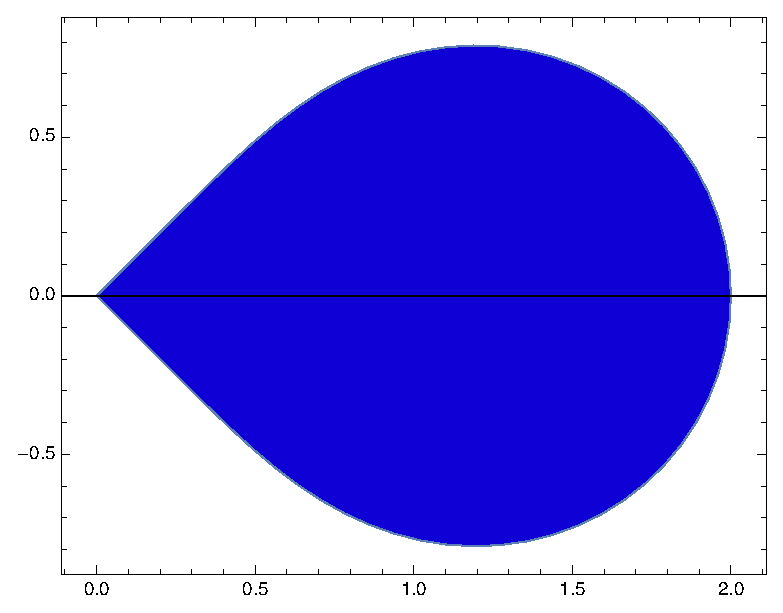
\includegraphics[width=0.8\columnwidth]{bdf2stability.eps}
\[
\left\lbrace \nicefrac{1}{\omega(\zeta)^\alpha} \,:\; |\zeta| \leq 1 \right\rbrace
\]
}
\end{column}
\end{columns}

\end{frame}

\begin{frame}{A worked out example}
Now we need to expand the convolution coefficients of \[\omega^\alpha(\zeta) = (\omega(\zeta))^\alpha = \frac{2^\alpha}{3^\alpha}\alert<2>{(1 - \nicefrac{4\zeta}{3} + \nicefrac{\zeta^2}{3})^{-\alpha}}.\]
\begin{onlyenv}<2>
\begin{alertblock}{Theorem~\parencite[Theorem 1.6c, p. 42]{HenriciBook}}\small
	Let $\phi(\zeta) = 1 + \sum_{n=1}^{+\infty} a_n \zeta^n$ be a formal power series. Then for any $\alpha \in \mathbb{C}$, we have\vspace{-0.5em}
	\[
	(\phi(\zeta))^\alpha = \sum_{n=0}^{+\infty} v_n^{(\alpha)} \zeta^n,
	\]
	where coefficients $v_n^{(\alpha)}$ can be evaluated recursively as\vspace{-0.5em}
	\[
	v_0^{(\alpha)} = 1, \qquad v_n^{(\alpha)} = \sum_{j=1}^{n} \left( \frac{(\alpha +1)j}{n} - 1 \right) a_j v_{n-j}^{(\alpha)}
	\]
\end{alertblock}
\end{onlyenv}
\only<3->{
	\vspace{-0.5em}\begin{itemize}
		\item $\omega_n = \nicefrac{2^\alpha}{3^\alpha} \tilde{\omega}_n$,
		\item<4-> $a_1 = -\nicefrac{4}{3}$, $a_2 = \nicefrac{1}{3}$, $a_j = 0$ if $j \geq 3$, thus using
		\[
		\tilde{\omega}_0^{(\alpha)} = 1, \qquad \tilde{\omega}_n^{(\alpha)} = \sum_{j=1}^{n} \left( \frac{(\alpha +1)j}{n} - 1 \right) a_j v_{n-j}^{(\alpha)}
		\]
		\item<5-> we get $\tilde{\omega}_0 = 1$, $\tilde{\omega}_1 = \nicefrac{4}{3}\alpha \tilde{\omega}_0 = \nicefrac{4 \alpha}{3}$, 
		\[
		\tilde{\omega}_n = \frac{4}{3} \left(1 + \frac{\alpha-1}{n}\right) \tilde{\omega}_{n-1} + \frac{4}{3}\left(\frac{2(1-\alpha)}{n} - 1\right)\tilde{\omega}_{n-2}.
		\]
	\end{itemize}	
}
\end{frame}

\begin{frame}[fragile]{A worked out example}
\begin{columns}
\begin{column}{0.4\columnwidth}
% This file was created by matlab2tikz.
%
%The latest updates can be retrieved from
%  http://www.mathworks.com/matlabcentral/fileexchange/22022-matlab2tikz-matlab2tikz
%where you can also make suggestions and rate matlab2tikz.
%
\definecolor{mycolor1}{rgb}{0.00000,0.44700,0.74100}%
%
\begin{tikzpicture}

\begin{axis}[%
width=0.8\columnwidth,
height=1.5in,
at={(0.758in,0.481in)},
scale only axis,
xmin=1,
xmax=258,
ymin=0.0351932463839126,
ymax=0.816496580927726,
axis background/.style={fill=white}
]
\addplot [color=mycolor1, only marks, mark=o, mark options={solid, mycolor1}, forget plot]
  table[row sep=crcr]{%
1	0.816496580927726\\
2	0.544331053951817\\
3	0.408248290463863\\
4	0.332646755192777\\
5	0.286025808442274\\
6	0.254525168745989\\
7	0.231634703900021\\
8	0.214064347091648\\
9	0.200020311893721\\
10	0.188450956579753\\
11	0.178698451432904\\
12	0.170328042254074\\
13	0.163039082720151\\
14	0.156615836639966\\
15	0.150898740552291\\
16	0.145766783090518\\
17	0.141126238402662\\
18	0.136903200100537\\
19	0.133038480633192\\
20	0.1294840344745\\
21	0.12620039261634\\
22	0.123154785794442\\
23	0.120319747475438\\
24	0.11767205775814\\
25	0.115191933851807\\
26	0.112862401750423\\
27	0.110668802977538\\
28	0.108598403334667\\
29	0.106640079600236\\
30	0.104784066448922\\
31	0.103021750361844\\
32	0.101345500544918\\
33	0.0997485292441923\\
34	0.098224775599067\\
35	0.096768808482516\\
36	0.0953757447639898\\
37	0.0940411801814675\\
38	0.0927611305855011\\
39	0.0915319817641304\\
40	0.0903504464053593\\
41	0.0892135270270474\\
42	0.0881184839200594\\
43	0.0870628073223882\\
44	0.086044193179562\\
45	0.0850605219574325\\
46	0.0841098400631279\\
47	0.0831903435029334\\
48	0.0823003634655442\\
49	0.0814383535681634\\
50	0.0806028785433848\\
51	0.0797926041783346\\
52	0.0790062883454532\\
53	0.0782427729876173\\
54	0.0775009769398495\\
55	0.0767798894863214\\
56	0.0760785645652497\\
57	0.075396115546058\\
58	0.0747317105131879\\
59	0.0740845679994707\\
60	0.0734539531192726\\
61	0.0728391740578784\\
62	0.0722395788789629\\
63	0.071654552616636\\
64	0.0710835146225571\\
65	0.0705259161420908\\
66	0.0699812380964912\\
67	0.0694489890507312\\
68	0.068928703348886\\
69	0.0684199394009815\\
70	0.0679222781069792\\
71	0.0674353214051071\\
72	0.0669586909331064\\
73	0.0664920267921565\\
74	0.0660349864043002\\
75	0.0655872434551208\\
76	0.0651484869142568\\
77	0.064718420127068\\
78	0.0642967599714255\\
79	0.063883236074178\\
80	0.0634775900823659\\
81	0.0630795749847179\\
82	0.0626889544793822\\
83	0.0623055023842133\\
84	0.0619290020862692\\
85	0.061559246027477\\
86	0.0611960352236887\\
87	0.0608391788145969\\
88	0.0604884936421965\\
89	0.0601438038556774\\
90	0.0598049405408109\\
91	0.0594717413720557\\
92	0.0591440502857552\\
93	0.0588217171729323\\
94	0.0585045975903064\\
95	0.0581925524882691\\
96	0.0578854479546558\\
97	0.0575831549732395\\
98	0.057285549195957\\
99	0.0569925107279557\\
100	0.0567039239246154\\
101	0.0564196771997644\\
102	0.0561396628443688\\
103	0.0558637768550246\\
104	0.0555919187716326\\
105	0.0553239915236806\\
106	0.0550599012845991\\
107	0.0547995573336929\\
108	0.054542871925189\\
109	0.0542897601639696\\
110	0.0540401398875913\\
111	0.0537939315542192\\
112	0.0535510581361256\\
113	0.0533114450184336\\
114	0.0530750199027996\\
115	0.0528417127157544\\
116	0.0526114555214387\\
117	0.0523841824384855\\
118	0.0521598295608186\\
119	0.0519383348821524\\
120	0.0517196382239878\\
121	0.0515036811669167\\
122	0.051290406985056\\
123	0.0510797605834434\\
124	0.0508716884382397\\
125	0.0506661385395883\\
126	0.0504630603369954\\
127	0.0502624046870982\\
128	0.0500641238037016\\
129	0.0498681712099644\\
130	0.0496745016926302\\
131	0.0494830712581975\\
132	0.0492938370909343\\
133	0.0491067575126454\\
134	0.0489217919441071\\
135	0.0487389008680879\\
136	0.0485580457938789\\
137	0.048379189223261\\
138	0.0482022946178418\\
139	0.0480273263676962\\
140	0.0478542497612507\\
141	0.0476830309563526\\
142	0.0475136369524706\\
143	0.0473460355639734\\
144	0.0471801953944382\\
145	0.0470160858119429\\
146	0.0468536769252964\\
147	0.0466929395611661\\
148	0.0465338452420637\\
149	0.046376366165149\\
150	0.0462204751818189\\
151	0.0460661457780456\\
152	0.0459133520554318\\
153	0.0457620687129535\\
154	0.0456122710293595\\
155	0.0454639348462009\\
156	0.0453170365514641\\
157	0.045171553063781\\
158	0.0450274618171943\\
159	0.0448847407464532\\
160	0.0447433682728189\\
161	0.0446033232903592\\
162	0.0444645851527113\\
163	0.0443271336602956\\
164	0.044190949047961\\
165	0.0440560119730453\\
166	0.0439223035038348\\
167	0.0437898051084059\\
168	0.0436584986438358\\
169	0.0435283663457663\\
170	0.0433993908183078\\
171	0.043271555024271\\
172	0.0431448422757124\\
173	0.0430192362247837\\
174	0.0428947208548713\\
175	0.0427712804720175\\
176	0.0426488996966106\\
177	0.0425275634553364\\
178	0.0424072569733785\\
179	0.0422879657668618\\
180	0.0421696756355269\\
181	0.0420523726556298\\
182	0.0419360431730568\\
183	0.0418206737966488\\
184	0.0417062513917255\\
185	0.0415927630738039\\
186	0.0414801962025042\\
187	0.0413685383756351\\
188	0.0412577774234545\\
189	0.0411479014030977\\
190	0.041038898593168\\
191	0.0409307574884839\\
192	0.0408234667949788\\
193	0.0407170154247454\\
194	0.0406113924912228\\
195	0.0405065873045199\\
196	0.0404025893668705\\
197	0.0402993883682166\\
198	0.0401969741819148\\
199	0.0400953368605623\\
200	0.0399944666319386\\
201	0.0398943538950585\\
202	0.0397949892163337\\
203	0.0396963633258386\\
204	0.0395984671136779\\
205	0.0395012916264519\\
206	0.0394048280638169\\
207	0.0393090677751373\\
208	0.0392140022562272\\
209	0.0391196231461782\\
210	0.0390259222242701\\
211	0.0389328914069636\\
212	0.038840522744971\\
213	0.0387488084204027\\
214	0.0386577407439882\\
215	0.0385673121523678\\
216	0.0384775152054545\\
217	0.0383883425838621\\
218	0.0382997870864001\\
219	0.0382118416276299\\
220	0.0381244992354845\\
221	0.0380377530489462\\
222	0.0379515963157827\\
223	0.0378660223903399\\
224	0.0377810247313882\\
225	0.0376965969000228\\
226	0.037612732557614\\
227	0.0375294254638094\\
228	0.0374466694745822\\
229	0.0373644585403291\\
230	0.0372827867040117\\
231	0.037201648099344\\
232	0.0371210369490224\\
233	0.0370409475629975\\
234	0.0369613743367875\\
235	0.0368823117498306\\
236	0.0368037543638764\\
237	0.0367256968214144\\
238	0.0366481338441395\\
239	0.0365710602314528\\
240	0.0364944708589969\\
241	0.0364183606772247\\
242	0.0363427247100013\\
243	0.036267558053237\\
244	0.0361928558735523\\
245	0.0361186134069717\\
246	0.0360448259576484\\
247	0.0359714888966161\\
248	0.0358985976605695\\
249	0.0358261477506715\\
250	0.0357541347313872\\
251	0.035682554229343\\
252	0.035611401932211\\
253	0.0355406735876179\\
254	0.0354703650020776\\
255	0.0354004720399467\\
256	0.0353309906224026\\
257	0.0352619167264441\\
258	0.0351932463839126\\
};
\end{axis}
\end{tikzpicture}%
\[\alpha = 0.5.\]
\end{column}
\begin{column}{0.6\columnwidth}
\begin{itemize}
	\item Since the $a_j$ are a finite small number, we can compute the coefficients in an $O(N)$ operations,
	\begin{onlyenv}<1>\definecolor{bg}{rgb}{0.95,0.95,0.95}
\begin{minted}[bgcolor=bg,fontsize=\scriptsize,breaklines]{matlab}
omega = zeros(1,N+1) ;
onethird = 1/3 ; fourthird = 4/3;
twothird_oneminusalpha = 2/3*(1-alpha);
fourthird_oneminusalpha = 4/3*(1-alpha);
omega(1) = 1 ; omega(2) = fourthird*alpha*omega(1);
for n = 2 : N
 omega(n+1) = (fourthird - fourthird_oneminusalpha/n)*omega(n) + ...
 (twothird_oneminusalpha/n - onethird)*omega(n-1);
end
omega = omega*((2/3)^(alpha)); 
\end{minted}
	\end{onlyenv}
	\item<2-> We can solve ${}_{CA}D^{0.5}_{[0,2]}y(t) = -2 y(t)$, $y(0) = 1$
	\only<2>{\begin{center}
	\begin{tabular}{ccc}
	\toprule
	$\tau$ & $|y^{(n)} - y(2)|$ & order \\
	\midrule
	 $2^{-6}$ & 1.44e-04 & 1.61 \\
	 $2^{-7}$ & 4.42e-05 & 1.71 \\
	 $2^{-8}$ & 1.28e-05 & 1.79 \\
	 $2^{-9}$ & 3.57e-06 & 1.84 \\
	 $2^{-10}$ & 9.68e-07 & 1.88 \\
	 $2^{-11}$ & 2.85e-07 & 1.76 \\
	 $2^{-12}$ & 8.17e-08 & 1.80 \\
	 $2^{-13}$ & 2.29e-08 & 1.84 \\
	 $2^{-14}$ & 6.27e-09 & 1.87 \\
	\bottomrule
	\end{tabular}
	\end{center}}
	\only<3->{
	\item<3-> For the starting weights we have to solve a $3 \times 3$ Vandermonde system:
	\[
	\left[\begin{array}{ccc} 1 & 1 & 1\\ 0 & 1 & \sqrt{2}\\ 0 & 1 & 2 \end{array}\right] \begin{bmatrix}
	w_{n,0} \\ w_{n,1} \\ w_{n,2} 
	\end{bmatrix} = \begin{bmatrix}
	b_1 \\ b_2 \\ b_3
	\end{bmatrix}
	\]
	number of time-step times.\vspace{-0.5em}
	\begin{block}{\small Reuse}\small
	Since we have a fixed time-grid we can reuse the same factorization for the Vandermonde system and
	compute all the weights in a single sweep.
	\end{block}
	}
\end{itemize}
\end{column}
\end{columns}
\end{frame}

\subsection{Fractional Brusselator}

\begin{frame}[fragile]{Fractional Brusselator}
The Brusselator is a model of the \textbf{autocatalytic chemical reaction}, it is described by
\only<1-3>{\[
\begin{cases}
\dot{x}_1 = a - (\mu + 1)x_1 + x_1^2x_2,\\
\dot{x}_2 = \mu x_1 - x_1^2x_2,
\end{cases}\quad a,\mu > 0.
\]}\only<4->{\[
\begin{cases}
{}_{CA}D^{\alpha_1} x(t) = a - (\mu + 1)x_1 + x_1^2x_2,\\
{}_{CA}D^{\alpha_2} x(t) = \mu x_1 - x_1^2x_2,
\end{cases}\quad a,\mu > 0.
\]}\vspace{-1em}
\begin{columns}
\begin{column}{0.6\columnwidth}
\begin{onlyenv}<1-2>
\begin{itemize}
	\item<1-> If $\mu > a^2 + 1$ then a single Brusselator has a \emph{unique limit cycle},
	\item<2-> If $(a-1)^2 < \mu \leq a^2 + 1$ all the orbits tend to the steady state.
\end{itemize}
\end{onlyenv}
\begin{onlyenv}<3>\definecolor{bg}{rgb}{0.95,0.95,0.95}
\begin{minted}[bgcolor=bg,fontsize=\small,breaklines]{matlab}
a = 1 ; mu = 4 ;
param = [ a , mu ] ;
f_fun = @(t,y,par) [ ...
par(1) - (par(2)+1)*y(1) + y(1)^2*y(2) ; ...
par(2)*y(1) - y(1)^2*y(2) ] ;
t0 = 0 ; T = 100 ;
y0 = [ 1 ; 1] ;
[T,Y] = ode45(@(t,y) f_fun(t,y,param),[t0,T],y0);
figure(1)
plot(Y(:,1),Y(:,2),'k-',y(1,1),y(2,1),'ro')
\end{minted}
\end{onlyenv}
\begin{onlyenv}<4->\definecolor{bg}{rgb}{0.95,0.95,0.95}
\begin{minted}[bgcolor=bg,fontsize=\small,breaklines]{matlab}
alpha = [0.8,0.7] ;
h = 1e-2;
[t, y] = fde_pi1_ex(alpha,f_fun,t0,T,y0,h,param) ;
\end{minted}

The cycle of the single fractional Brusselator is contained in the region
\[
\left\lbrace (x_1,x_2) \,:\; \frac{a}{\mu+1} < x_1 < \frac{2a}{\mu}, \; 0 < x_2 < \frac{\mu(1+\mu)}{a} \right\rbrace
\]
\end{onlyenv}
\end{column}
\begin{column}{0.4\columnwidth}
\begin{onlyenv}<3>
\centering

% This file was created by matlab2tikz.
%
%The latest updates can be retrieved from
%  http://www.mathworks.com/matlabcentral/fileexchange/22022-matlab2tikz-matlab2tikz
%where you can also make suggestions and rate matlab2tikz.
%
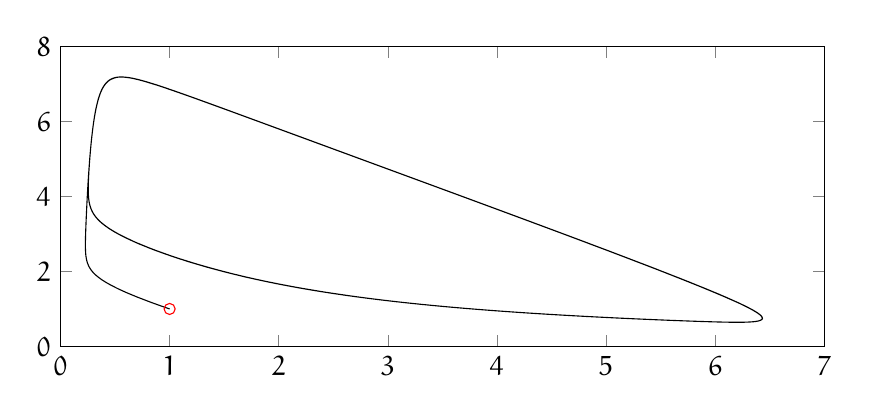
\begin{tikzpicture}

\begin{axis}[%
width=0.8\columnwidth,
height=1.5in,
at={(0.772in,0.481in)},
scale only axis,
xmin=0,
xmax=7,
ymin=0,
ymax=8,
axis background/.style={fill=white}
]
\addplot [color=black, forget plot]
  table[row sep=crcr]{%
1	1\\
0.951396478514415	1.04901485344908\\
0.905886874936536	1.09572352920837\\
0.863230843230182	1.14031665691579\\
0.823216568740605	1.18295989371498\\
0.703612488311578	1.31619951476378\\
0.60706175828555	1.43258030737522\\
0.529248622658646	1.53528720287898\\
0.466569583210125	1.62687918781389\\
0.417975818900003	1.70617938397315\\
0.378715945700655	1.77855971628543\\
0.347169955237837	1.84519642290188\\
0.321860218935474	1.90715728970332\\
0.300716093546687	1.96789895995543\\
0.284017032802825	2.02528218986367\\
0.270918094719887	2.07993631041816\\
0.26064433814963	2.13243546405941\\
0.25204539433087	2.18687090513522\\
0.245474779616495	2.23974515785039\\
0.240515902250636	2.2913722331529\\
0.236782415391894	2.34204121140277\\
0.233624368383481	2.39906928880999\\
0.231416610014351	2.45533610259257\\
0.229947467618426	2.51100131582995\\
0.229011036938055	2.56621853422728\\
0.228371008680295	2.63196111355016\\
0.228157242144286	2.69731374969204\\
0.228270606940813	2.76235032612992\\
0.228601172086644	2.82715137366094\\
0.229199294778509	2.90801046421169\\
0.229979886304314	2.98861470408042\\
0.230906717539374	3.06898922272656\\
0.23192119424655	3.14917431253556\\
0.233310279795477	3.25371683024993\\
0.234795177895461	3.35796582252296\\
0.236375338289671	3.46191626165326\\
0.238013734253338	3.56558763997107\\
0.2402049690552	3.70169786543635\\
0.242508719615824	3.83728858793963\\
0.244958801839965	3.97231975695592\\
0.247504207330612	4.1068051817766\\
0.2505543476487	4.2647895187035\\
0.253799415265815	4.42190736107296\\
0.257311601484864	4.57807317893655\\
0.261012934592969	4.73328410455831\\
0.265083073919846	4.897373820359\\
0.269462642733442	5.06019487094776\\
0.274236027100128	5.22162092160058\\
0.279375259134319	5.38155838130038\\
0.285435725019402	5.55518469949374\\
0.292103284325351	5.72661874527788\\
0.29951731963326	5.89558196684794\\
0.307834777527837	6.06167993884782\\
0.320259323230986	6.26804066620669\\
0.334953517702971	6.46787157526594\\
0.35288400344813	6.65920811815264\\
0.376518639625773	6.83821363482431\\
0.392245927191027	6.92403182433029\\
0.411241934247868	7.00375853934537\\
0.435050226990416	7.0751608083717\\
0.466369401374797	7.13452176812091\\
0.49097361307035	7.16217986992705\\
0.521553608382587	7.18114912455481\\
0.561224289183914	7.18753276327254\\
0.615589900362173	7.17452894348682\\
0.656668180614308	7.15423748614257\\
0.7083535975445	7.12074294610669\\
0.776051231970696	7.06785610111144\\
0.869268164305131	6.98487930825982\\
0.954909324350128	6.90267811343794\\
1.06698163872771	6.79034213170275\\
1.22150841240765	6.63045922092703\\
1.44804097171063	6.39126720932649\\
1.62754937896681	6.20002252820236\\
1.86277943937826	5.94857150411881\\
2.17888375828312	5.61023338054971\\
2.61197158937562	5.14672187658688\\
2.82464497940801	4.91918678207554\\
3.0653358506728	4.66167077025103\\
3.33580680466969	4.37216213118909\\
3.63620277776386	4.05025807605247\\
3.96450050510089	3.69773035625773\\
4.31412777617747	3.32092543703621\\
4.67423613649811	2.93055349250191\\
5.030034833519	2.54138363198729\\
5.42427525075667	2.10339739555065\\
5.76122736787513	1.71892427686373\\
6.02582141014913	1.40371259359416\\
6.21475095252361	1.16180877011237\\
6.29196060671814	1.05337993608577\\
6.34939318118831	0.964328836734549\\
6.3896207246701	0.892188925318978\\
6.41533567856711	0.834366247150825\\
6.42918546383076	0.788298035027014\\
6.43323743437459	0.751974740222845\\
6.4292904706007	0.723647349131883\\
6.41899177965069	0.701714407248495\\
6.40093880181673	0.682490013360429\\
6.3776957662883	0.668598022307626\\
6.35044881848496	0.658880882488195\\
6.32026988397509	0.652293749500934\\
6.28353745634293	0.647582807400436\\
6.2447842363785	0.645187668771465\\
6.20456578241967	0.644564379860184\\
6.16339629827039	0.645210243612686\\
6.11155594467944	0.64721872763565\\
6.05916107281093	0.650287170460484\\
6.00647466406597	0.654154795245971\\
5.95376968344926	0.658552026821793\\
5.88550422976011	0.664752720631789\\
5.81762212186716	0.671428720135841\\
5.75021110696584	0.678484811324392\\
5.68341208600311	0.685775248647736\\
5.59474586176547	0.695761393513183\\
5.50729029199374	0.706030137121967\\
5.42101392932561	0.716589268948924\\
5.33600772035996	0.727330184082837\\
5.22752276578067	0.741401208550409\\
5.12108523711687	0.755793730942614\\
5.01655616778102	0.770595610949635\\
4.91404590587435	0.785659953375352\\
4.79511056963078	0.803688386935884\\
4.67881457684365	0.822155522602549\\
4.56496725427778	0.841174314070751\\
4.45366689260735	0.860591176603166\\
4.3268147362868	0.883617086868462\\
4.20318562675394	0.907254209015245\\
4.08256417759994	0.93160891642098\\
3.96498417321559	0.956567352764769\\
3.82644044492984	0.987511347693758\\
3.69202672784297	1.01939497179444\\
3.56148482499805	1.05231071754835\\
3.43472865775077	1.08621850883641\\
3.27532782389068	1.13177590773604\\
3.12178124512129	1.17904065395073\\
2.97373786638606	1.2280675837926\\
2.83082780051434	1.2789911344375\\
2.59752729403618	1.37091422101302\\
2.3777464036942	1.46799291824174\\
2.17090462342823	1.5697081410344\\
1.97450334827402	1.6776222872215\\
1.78395855541008	1.79444287178265\\
1.60360084844119	1.91664354925967\\
1.4333481771201	2.0434471544074\\
1.27341966391916	2.17378142154198\\
1.04424292747537	2.38237764538931\\
0.845998806857754	2.58826472841902\\
0.68131792050286	2.78447891639065\\
0.55118384189968	2.96563969363475\\
0.498770308026105	3.0494260832008\\
0.45394086872441	3.12883325993\\
0.416044209541832	3.20404399812068\\
0.384336111432676	3.27536025023886\\
0.358013593769809	3.34318473584911\\
0.336354142825794	3.40792708661933\\
0.318685997077828	3.46998412876552\\
0.304365975827167	3.52974618446269\\
0.290213750569338	3.60210644615339\\
0.279529171240426	3.67202723516655\\
0.271602484551351	3.73998439566168\\
0.265781426555056	3.80640425532247\\
0.261401795947338	3.87399733975016\\
0.258359699868575	3.94057132877896\\
0.256362254805804	4.00632737188647\\
0.255141414008558	4.0714445606818\\
0.254411369685204	4.14889331344373\\
0.254317772276626	4.22574832890976\\
0.254713474762368	4.30210799526093\\
0.255454938814692	4.37806362913659\\
0.256716734131058	4.47295252011685\\
0.258290542590509	4.56734677973016\\
0.260117719992177	4.66127716301394\\
0.26212844253919	4.75477680055528\\
0.264997277806064	4.8781426979352\\
0.268110970087949	5.00075244497502\\
0.271471029005092	5.12257450474098\\
0.275051325243529	5.24358357031351\\
0.280102297123516	5.40226971616788\\
0.28560374032759	5.55931451610883\\
0.291640183826371	5.7145458300451\\
0.298275484302544	5.86774784986904\\
0.307764623834909	6.05850064411772\\
0.318642219083026	6.24496409256483\\
0.331326921535864	6.42624358566908\\
0.346738734896425	6.60076564282938\\
0.361798351673154	6.73259715903926\\
0.380094443535604	6.85746544531378\\
0.403349367073131	6.97265816201022\\
0.434861600361392	7.07338456994502\\
0.453053125729116	7.11186550310835\\
0.474877526910602	7.14469728669945\\
0.501808117922334	7.16995255373952\\
0.536233380263818	7.18459737303299\\
0.583763186159059	7.18198190071629\\
0.64670932038628	7.15869907763502\\
0.741517380068853	7.0955340600624\\
0.909056790570504	6.94631844902843\\
0.978833756132025	6.87817340914933\\
1.06508994833858	6.79134424000144\\
1.17450994929914	6.67856915515692\\
1.31761463395991	6.52850939948647\\
1.51102020291456	6.32337681572976\\
1.78010923780511	6.03613426304222\\
2.17234773919648	5.61636100167903\\
2.76309282021136	4.98410191494463\\
2.89837740402029	4.83936494935512\\
3.04385596841627	4.68370892763147\\
3.1999053072762	4.51670354983676\\
3.36671542553336	4.3381037211764\\
3.5442345375825	4.14790556898764\\
3.73205433788006	3.94646247109566\\
3.92929267348494	3.73460583661968\\
4.13453767644409	3.51370270711218\\
4.63786566358259	2.96922161595724\\
5.13256902585205	2.42726698529296\\
5.57491277318923	1.93194101366653\\
5.92956573938655	1.51941581905619\\
6.06528213866877	1.35370303372442\\
6.17575056469467	1.21250042048264\\
6.26251658576737	1.09440578158571\\
6.32794215013725	0.997195133871861\\
6.37496671510542	0.918055626800744\\
6.40626230461435	0.854410596608738\\
6.42433777980116	0.803833690164178\\
6.43161637242198	0.763978139572005\\
6.42968530158631	0.729454327485256\\
6.41922260256023	0.703503877641057\\
6.40204849676544	0.684353243988176\\
6.37981704564697	0.670392496312602\\
6.35207852529972	0.659776933783203\\
6.32107588083546	0.652635460921637\\
6.28760511964148	0.648190315586531\\
6.25238700215469	0.645738114933858\\
6.20836352924076	0.644670908131988\\
6.1630983405716	0.645230241806787\\
6.11699387218772	0.647020680280863\\
6.07043755121714	0.649662348894034\\
6.01135660746855	0.653796046311887\\
5.95219910685008	0.658650606539768\\
5.89313430975284	0.664054774800935\\
5.83436104565191	0.669809490833777\\
5.7569591495644	0.677760045078123\\
5.6803246916829	0.686058352855675\\
5.6044864167914	0.694661894818442\\
5.52955204715918	0.70345293713554\\
5.43077718553519	0.71535392474971\\
5.33361999780771	0.727536457359786\\
5.2379963139675	0.740049166536415\\
5.14400129920992	0.752770747159316\\
5.02954492506568	0.768699282565366\\
4.91744553250512	0.785001052263375\\
4.80753123498915	0.801783653922647\\
4.69991576947112	0.818887904876434\\
4.57749303840739	0.839033229042277\\
4.45796102460469	0.859687213992619\\
4.34111827249275	0.880960652632245\\
4.22703735349031	0.902715553914869\\
4.09533100063533	0.928978723936743\\
3.96721899661892	0.955979321943888\\
3.84246912575161	0.983818469912815\\
3.72106870441941	1.01241097025959\\
3.57449025784141	1.04897138360537\\
3.43268985770084	1.0867430030132\\
3.29537571688519	1.12580604734187\\
3.16236313412356	1.16618104496118\\
2.98410117365212	1.22461246576633\\
2.81338611706284	1.28557908439267\\
2.64977445318382	1.3490772882239\\
2.49255528227962	1.41545336889496\\
2.26390145138482	1.52272970160173\\
2.0484409175425	1.63637227446745\\
1.845548845856	1.75587823562489\\
1.65369241492626	1.88174317818824\\
1.45701775564082	2.0253573022878\\
1.27375718936942	2.1737553891085\\
1.10473297562893	2.32477014172376\\
0.95124672102743	2.47568963722971\\
0.821368282076785	2.6160112369889\\
0.707690642237531	2.75118931027305\\
0.610538773808827	2.87942669293677\\
0.529524941591259	2.9996224755869\\
0.463483730552281	3.11144405212153\\
0.410781504762594	3.21531638428841\\
0.369652215571176	3.31195133824198\\
0.338141212350296	3.40226642374864\\
0.315734450158789	3.48135582517451\\
0.298596219061499	3.55684112462715\\
0.285696435442135	3.62938909730511\\
0.276074864481561	3.69960582610444\\
0.269100084499153	3.7660175940702\\
0.263977209024161	3.83107138802785\\
0.26031602032535	3.89503422499696\\
0.257761826722332	3.95814330793991\\
0.25580977098267	4.03084038769253\\
0.254730893370839	4.10280871888166\\
0.254324905519659	4.17418481446046\\
0.254402958154089	4.2450925080014\\
0.254954647728652	4.3315636069601\\
0.255915122583738	4.41753812679909\\
0.257195139343081	4.50307137949388\\
0.258700023960172	4.58821775175542\\
0.260887968498952	4.69854864904949\\
0.263321166513893	4.80828404283482\\
0.265976883556039	4.9174209936455\\
0.268812206645772	5.02596237846243\\
0.272835449215541	5.17013820857172\\
0.277181518559966	5.31314362397388\\
0.281893747422718	5.45488379233628\\
0.28697983142104	5.59525825914107\\
0.294069204471857	5.77208631366067\\
0.301970253946831	5.94617078882746\\
0.310873545375781	6.11710578416314\\
0.32108893987303	6.28425755796065\\
0.333163265104771	6.44767947511421\\
0.347432122891503	6.60551115654982\\
0.364815281218107	6.7560917615394\\
0.387093370227086	6.89661554033581\\
0.404616625362028	6.97669421828271\\
0.42607790964152	7.04974184346998\\
0.453531149043709	7.11286965935225\\
0.490725357362015	7.16105479776562\\
0.515699196738154	7.17745299670838\\
0.546369598170736	7.18587308125364\\
0.58536183318939	7.18309107478694\\
0.637142105969488	7.16375727279529\\
0.684121752927665	7.13625007921083\\
0.744158573737531	7.09269296213674\\
0.824666602410595	7.02467125462341\\
0.939284980459826	6.91697630163595\\
1.05457236269777	6.80190069368763\\
1.21147940711869	6.63995133802269\\
1.44259867019493	6.3960199613025\\
1.81345533928224	6.00026505373843\\
1.86182305202548	5.94851757971504\\
1.91288702215483	5.89387327245441\\
1.9668391244699	5.83612899350123\\
2.02388529946471	5.77506671765144\\
2.08424559451862	5.71045346124422\\
2.14815416664225	5.6420412513044\\
2.21585917622418	5.56956711547119\\
2.28762279188868	5.49275301721907\\
2.65417485930055	5.10050039796917\\
3.13264666134656	4.58881200770715\\
3.73391202870083	3.94470730345769\\
4.43407381260737	3.1902466940772\\
4.87191711333426	2.71392352220436\\
5.28788138523561	2.25497044715523\\
5.65377176437238	1.8419669931433\\
5.94895396008234	1.49616678801557\\
6.0923345919553	1.31983992102717\\
6.20593499953484	1.1724514476334\\
6.29202364631594	1.0519146560699\\
6.35388765611265	0.955117369789532\\
6.3954938478639	0.878250812976131\\
6.42020674583777	0.818060404921281\\
6.43106245899384	0.771603838240494\\
6.43094833884133	0.736082372333605\\
6.42225313006191	0.708706490537572\\
6.40670028853159	0.688268953495818\\
6.385773625034	0.673323107738024\\
6.36081352730903	0.662563449539924\\
6.32964903004945	0.654254309137464\\
6.29569021042206	0.64897996767732\\
6.25964590483372	0.646047415290196\\
6.22216231212392	0.64482572129208\\
6.1754108426418	0.644958719466692\\
6.12768585129843	0.646488771141977\\
6.07933486020401	0.649073599957729\\
6.03069950054206	0.652377589488159\\
5.96847149710879	0.657270613172939\\
5.90633599755209	0.662784106560634\\
5.84443121245953	0.668776054586581\\
5.78293311089988	0.675068726635574\\
5.7016434061192	0.683726659480427\\
5.62127563288967	0.692700394225676\\
5.54183685055876	0.70196599722106\\
5.46342610493267	0.711411947047957\\
5.36089458156895	0.724089993420558\\
5.26014042198579	0.737060141673666\\
5.16105875247209	0.750386308130698\\
5.06375000683915	0.763938242395026\\
4.94752413464095	0.780598439437782\\
4.83376023421441	0.79765416729834\\
4.72227809019733	0.815216509354167\\
4.61318804689864	0.833126232267184\\
4.48928732906488	0.854221781212002\\
4.36838737501934	0.87585881573613\\
4.2502822310992	0.89814670241467\\
4.13503195073079	0.920955256952533\\
4.00109411084573	0.948731765171549\\
3.87092379942484	0.97730858451733\\
3.74428059631918	1.00678419753359\\
3.62112892668781	1.0370874848566\\
3.47059651233378	1.07642838852613\\
3.32516832311009	1.11712605004805\\
3.18453494072178	1.15925371958199\\
3.04845824615419	1.20286475421757\\
2.85829265939583	1.26905963547189\\
2.67682278008713	1.33834799219714\\
2.50355015282186	1.41066856083117\\
2.33749681144757	1.48653726616608\\
2.12910534041289	1.5920939528675\\
1.93180805024554	1.70347756150558\\
1.74508675419952	1.82030176132677\\
1.56821663472705	1.942441730502\\
1.36317702411008	2.09963763871194\\
1.174141234281	2.26114779788502\\
1.00240507203664	2.42392844390405\\
0.849705956740064	2.5843954722854\\
0.734009149145527	2.71880268831741\\
0.634285541500797	2.84685827971864\\
0.550367551374787	2.96733308397406\\
0.481394708770969	3.07969835987693\\
0.42582332097446	3.18414121038241\\
0.38190727112018	3.28137285687151\\
0.347906062468668	3.37224300406064\\
0.322003565155732	3.45769062640378\\
0.303852775056665	3.53206773116707\\
0.289963693170026	3.60349329334107\\
0.27949668678564	3.6725197952685\\
0.27167650237927	3.73964632545436\\
0.265757127817327	3.80656750837238\\
0.261488088225813	3.87226308412946\\
0.258515446105761	3.93697582019515\\
0.256516675830252	4.00092148128759\\
0.255073576514531	4.07519435572255\\
0.254402699155431	4.14879867394998\\
0.25432597426989	4.22185512796672\\
0.254673713396978	4.29447397346425\\
0.255507321606628	4.38396311675277\\
0.256708006191678	4.47296238968898\\
0.258198826232569	4.56151746813364\\
0.259895166825267	4.64967445985172\\
0.262334404263635	4.76474459661522\\
0.265013996339746	4.87916846394052\\
0.267920277725451	4.99293311431606\\
0.271016724221546	5.10603188112238\\
0.275404988154215	5.2558567095822\\
0.280156316665697	5.40435240138895\\
0.285328154930637	5.55139915289903\\
0.290944160765586	5.69686174415334\\
0.298795284013098	5.8784705696554\\
0.30762440078651	6.05687487377788\\
0.317678506051082	6.23154352212511\\
0.329416714986942	6.40160718063999\\
0.341021498984843	6.5397511152953\\
0.354633325305552	6.67307454903484\\
0.371031616562856	6.80023382762051\\
0.391570535930198	6.9191019855564\\
0.411491808059311	7.00208068184499\\
0.436372138748343	7.0763466692653\\
0.469311567911893	7.1376136072473\\
0.516479839942598	7.17779387060921\\
0.540627748298994	7.18496079991099\\
0.569665015187886	7.18549100013822\\
0.605465443551186	7.17711765777372\\
0.650983040166252	7.15633646406023\\
0.712063927381487	7.11646538091382\\
0.793344605334666	7.05188995484541\\
0.911640124848986	6.94371835629755\\
1.10358596939462	6.75164438736302\\
1.23667185549504	6.61337723877323\\
1.41475698329491	6.42543921468981\\
1.66562222854567	6.15814722976475\\
2.03842987770583	5.75932412662114\\
2.1383804141008	5.65232982903194\\
2.24801504267034	5.53497345462753\\
2.36841910980917	5.40610350444983\\
2.50075661929961	5.26448231741119\\
2.64623828058645	5.10881799565691\\
2.80609752565439	4.93778784927104\\
2.98142848143199	4.75020134509043\\
3.17310800324191	4.54507853343649\\
3.5141735909048	4.17982594747559\\
3.89669931337446	3.76935316688795\\
4.31170684605401	3.32225519417412\\
4.7415286809167	2.85596796314402\\
5.16033752203419	2.39625695620998\\
5.53840654994231	1.97316088441034\\
5.85346963264893	1.6094935847447\\
6.0936173700427	1.31785204323759\\
6.19886879860984	1.18149188139464\\
6.28074495378138	1.06794233846217\\
6.34165838696324	0.974920336662668\\
6.38443635562766	0.899720919107698\\
6.41210824220924	0.839422628031736\\
6.42716649536802	0.791609214975965\\
6.43183262059203	0.754124759273118\\
6.42817961553992	0.724956849048366\\
6.41647522107712	0.700043467333035\\
6.39837101157101	0.681630652576173\\
6.3752799830596	0.668340369647937\\
6.34847912296882	0.658928602968278\\
6.31559640635996	0.651829185855332\\
6.28018263290045	0.647516891643304\\
6.24289382801763	0.645350099982421\\
6.20433005983211	0.644742723044131\\
6.15602552216909	0.645480925532383\\
6.10688126801978	0.647506181027696\\
6.05721793329721	0.650502172727373\\
6.00735529012006	0.654154347346172\\
5.94334550222931	0.659453293504813\\
5.87951847788072	0.665323604780581\\
5.81599631248604	0.671638328308879\\
5.7529433395187	0.678230477321336\\
5.66943703694861	0.687288482164157\\
5.58693951671339	0.696649099961104\\
5.50544608693641	0.706298242936348\\
5.42505230271653	0.716126396728171\\
5.32057172324959	0.729235327898714\\
5.21795432696782	0.742644245925895\\
5.11708424039885	0.756424974713185\\
5.01806506672287	0.770442028339108\\
4.9009544607872	0.78751582628659\\
4.78636155434467	0.804998027491596\\
4.6741024172591	0.823000784850598\\
4.56428439275738	0.841365931070647\\
4.43951410461409	0.863026594947769\\
4.31780977298739	0.885248727902109\\
4.19896273200245	0.908140827490396\\
4.08302545159164	0.931577434739277\\
3.94774976545278	0.960268348971795\\
3.81634620262836	0.989798734916383\\
3.68856929465007	1.02026541177139\\
3.56436925174986	1.05160599896521\\
3.41136769186764	1.09268258280928\\
3.26367655506876	1.13521037006849\\
3.12097509236849	1.17925790193726\\
2.98299017853676	1.22490005721082\\
2.78389959596994	1.29671360104151\\
2.59441294589485	1.37204832613815\\
2.41399591442951	1.45078486555286\\
2.24143669235203	1.53359119180843\\
2.03995465870185	1.64084042289762\\
1.84900069515184	1.7537807370215\\
1.66814558860369	1.87198620170358\\
1.49694999831352	1.99508195688575\\
1.28656937894848	2.16303353255008\\
1.09460605897528	2.33446370084195\\
0.922760563290066	2.5055349493139\\
0.773008332163539	2.67201299970127\\
0.674499504992622	2.79356726908754\\
0.589784216288154	2.90893797767615\\
0.518436367610051	3.01744362338631\\
0.459532584890602	3.11891928593966\\
0.411692728898456	3.21370516977106\\
0.373466222984135	3.30245202283728\\
0.343430883617401	3.38588850610925\\
0.320137598448523	3.46479705337725\\
0.302371212845732	3.5391051024961\\
0.288800671597034	3.61050282556937\\
0.278594719018634	3.67953841818607\\
0.270986149695279	3.74670649706887\\
0.265245340876514	3.81363166091278\\
0.26111754262767	3.87935610689549\\
0.25825617069405	3.94411761470033\\
0.256345340086093	4.0081275183722\\
0.254980137007687	4.08270995288533\\
0.254372309584726	4.15663228683719\\
0.254347075398405	4.23001285372014\\
0.254737522208418	4.30295990967596\\
0.255616464157157	4.39296643871228\\
0.256856096605906	4.48248356703784\\
0.258381452337227	4.57155540027855\\
0.26010953718739	4.66022668320876\\
0.262591502007555	4.77611559501107\\
0.265313595173127	4.89134854725175\\
0.268263665495337	5.0059108385217\\
0.271406236063919	5.1197940950549\\
0.275858397490429	5.27054837410146\\
0.280681291428115	5.41994468782046\\
0.285934881796383	5.56785859449804\\
0.291646030785873	5.71414812086872\\
0.299639446153431	5.8965950490048\\
0.308643707716926	6.07574832402604\\
0.31891780141408	6.2510506012038\\
0.330952808107985	6.42158277801799\\
0.343268484209359	6.5636898842028\\
0.35783715543425	6.70044725275276\\
0.37560626767533	6.83023891460522\\
0.398278331691133	6.95042880921883\\
0.417395846408004	7.02273111902298\\
0.441027524496934	7.08728660249368\\
0.471678502490259	7.1406597142869\\
0.514042241619757	7.17670713343667\\
0.540233082399084	7.18491841606294\\
0.572234918629314	7.18523112257779\\
0.612571896671663	7.17459531877827\\
0.665426490386297	7.1480660083658\\
0.717577002319799	7.11278496506427\\
0.784680244572235	7.05938079472356\\
0.875560434922583	6.97792440007765\\
1.00668380895625	6.85019675332736\\
1.20823578404929	6.64276725880117\\
1.53662558091064	6.29608558223318\\
2.2022563595231	5.58582222350324\\
3.61402422126052	4.07336312711841\\
3.81888939649768	3.85351874476744\\
4.03386496127136	3.62240458681148\\
4.25689056194597	3.38203114419827\\
4.48513304539737	3.13519532102458\\
4.71503463405883	2.8854346335445\\
4.94230835097103	2.63703886809602\\
5.16249016033409	2.39449890028991\\
5.37117271438751	2.16227328110547\\
5.66955838750498	1.82418852345019\\
5.91754660672319	1.53410658192224\\
6.11059700952116	1.29702399278293\\
6.25054746143845	1.11157534945916\\
6.32227046760194	1.00650039957482\\
6.3732353547431	0.921797239216457\\
6.40649938000861	0.854523674312427\\
6.42517100326285	0.801679279407821\\
6.43221659240698	0.760388816956676\\
6.42983177550491	0.72851428821034\\
6.41988185694445	0.704240224632004\\
6.40406487743519	0.685914854030636\\
6.38143563380326	0.67092571229333\\
6.35457047290289	0.660345171815658\\
6.32446222265143	0.653203850760702\\
6.29200780638402	0.648627048409569\\
6.2520638629743	0.645628187836482\\
6.21046175489811	0.644619574185541\\
6.16768636465988	0.645125863525456\\
6.1241929962478	0.646701479674249\\
6.06930353961913	0.649680626855657\\
6.01407844217842	0.653556077498686\\
5.9587369519824	0.658108998467073\\
5.90351679376823	0.663103501880918\\
5.83140636477625	0.670062770290334\\
5.75984609011732	0.677433237108265\\
5.68889710992889	0.685143783625721\\
5.61868399553377	0.693062914415434\\
5.52557859570434	0.703869135548552\\
5.43385966119891	0.714951991517308\\
5.34347296867081	0.726337252933729\\
5.25450928954343	0.737912984042015\\
5.14312678229554	0.752798597590077\\
5.03393516103574	0.768027232401201\\
4.92677895932184	0.783697343664212\\
4.82177199714657	0.799654637257386\\
4.7013352097593	0.818561770243682\\
4.58364387298266	0.83793615504148\\
4.4685025181355	0.857890180660362\\
4.3559993247153	0.878276223059038\\
4.22715900205991	0.90261890812558\\
4.10169293083966	0.927622755289219\\
3.979379013115	0.953392053931249\\
3.86023252136472	0.979824387371167\\
3.71847791157986	1.01300323779392\\
3.58110992205479	1.04722610221596\\
3.44785731413274	1.08258085282362\\
3.31859619387462	1.11905065277257\\
3.1522892798339	1.16939180361796\\
2.99243990514345	1.2217325760392\\
2.83866327395978	1.27611003590684\\
2.69047484852017	1.33272941924855\\
2.41415183728375	1.45151483977074\\
2.15749112675021	1.57766024301311\\
1.92023827167562	1.70950030294531\\
1.69715608889313	1.8505691189941\\
1.51182523878655	1.98243018002063\\
1.33793347693608	2.11877182048144\\
1.17598821766483	2.25803711749368\\
1.02690178102346	2.39822357495727\\
0.856622907173513	2.57533588192801\\
0.711321681078202	2.74535857671093\\
0.591754139017251	2.90469025671922\\
0.497053784106807	3.05132151938415\\
0.446093874439038	3.14266835737741\\
0.404195548640046	3.22849526960009\\
0.370250229039008	3.30928821140415\\
0.343078912796305	3.38563778745364\\
0.321484744672894	3.45822806451638\\
0.304509864571961	3.52767020856033\\
0.291325024607771	3.59449355742622\\
0.281159751717436	3.65918691214468\\
0.272809920539677	3.72711238950196\\
0.266637688516286	3.79345824270962\\
0.262184089812154	3.85853780049277\\
0.259030533383374	3.92262998121891\\
0.256626466298095	3.99372642295055\\
0.255177837484884	4.06404582899529\\
0.254467576391598	4.13373663188729\\
0.254293029676969	4.20293259877293\\
0.254587340387155	4.28713046927037\\
0.255332887181761	4.37081863054811\\
0.256428734747343	4.45406131401624\\
0.257770319816596	4.53692064840404\\
0.259746805190598	4.64337112212276\\
0.261976708859454	4.74926140479255\\
0.264429555190914	4.85459656871822\\
0.267056888486305	4.95938691356578\\
0.270788672556672	5.09870838296277\\
0.274815813375216	5.23697783602889\\
0.27917078391831	5.37411852862757\\
0.283850893933168	5.51005347762208\\
0.290379935419435	5.68290595416216\\
0.297608798184991	5.85333676560924\\
0.30569370173	6.02101741315378\\
0.314856152252541	6.18545744315016\\
0.326846482027438	6.36481911856478\\
0.341003537437154	6.53837528883984\\
0.358227800804296	6.70442327508893\\
0.380409454958068	6.85997071047847\\
0.396874578543226	6.94421541453545\\
0.416890338019415	7.02195235952698\\
0.4422127665152	7.09066869587506\\
0.475975538876824	7.14609614317559\\
0.500552552468131	7.16884509812507\\
0.530916976572122	7.18330965289273\\
0.569908284006578	7.18596361956421\\
0.622495363080239	7.17080553168595\\
0.666010229740734	7.14789544451802\\
0.721192321832582	7.11052465615714\\
0.794330579768258	7.05151561530248\\
0.896750203530038	6.95817097337708\\
0.991066837309914	6.86607619801322\\
1.11583275451697	6.73944422745678\\
1.29074016389981	6.55694832958335\\
1.55289873489511	6.2788277795166\\
1.69427740962186	6.12791397268369\\
1.86600510381408	5.94426568373355\\
2.07707561444256	5.7183516978886\\
2.33927220965176	5.43769199176934\\
2.66601213100024	5.08803028612457\\
3.07655189690134	4.64889228994662\\
3.58007331340529	4.10973890529154\\
4.16782154555424	3.47800376691012\\
4.65068175854419	2.95544641779941\\
5.12489150702209	2.4359385787619\\
5.55162915358756	1.95862676640281\\
5.89898954018541	1.55614588322176\\
6.04709052243595	1.37652547471542\\
6.16688596574653	1.22436289104381\\
6.26004181717387	1.0981616525092\\
6.32928497388537	0.995358689117286\\
6.37810050699948	0.912619366054999\\
6.40961265436382	0.846929425275635\\
6.42672592794594	0.795478777716945\\
6.43224237587736	0.755553812323795\\
6.42830356562216	0.723275015592604\\
6.41638469510564	0.699029296741301\\
6.39819107730587	0.681154780093966\\
6.37526892213784	0.66814618624302\\
6.34659335158048	0.658158264185122\\
6.31477824963867	0.651528033689236\\
6.28059726598852	0.647499462092309\\
6.24475215598043	0.645387630951783\\
6.20001348765501	0.644651927972631\\
6.15410742304198	0.645478216164096\\
6.10742109286038	0.647485889690988\\
6.06032906094636	0.650307517750415\\
6.00042744946774	0.654645236738212\\
5.94049476456301	0.659675740012449\\
5.88069180376937	0.665235768162121\\
5.8212111086894	0.671132153538587\\
5.74279882397636	0.679267534069377\\
5.66519450753002	0.687741164257217\\
5.58842109832909	0.696515552615731\\
5.51258373565629	0.705474924085697\\
5.41279278960157	0.717580094415096\\
5.31466205520264	0.729969063635744\\
5.21810182658316	0.742694598457861\\
5.12320855078379	0.755633153251781\\
5.0082606618158	0.771752819518041\\
4.89569808688935	0.788251475708784\\
4.78534651267902	0.805237857897468\\
4.67731905676947	0.822552499458772\\
4.55451817259026	0.842939362561125\\
4.43463605013406	0.863843140228295\\
4.31747009372672	0.885374270194736\\
4.20308972523398	0.907396724388846\\
4.07081837870693	0.934041597624668\\
3.94218507711086	0.961439530769732\\
3.81695555351687	0.989690992953901\\
3.69511142403525	1.01871429330402\\
3.54754985838763	1.05596578870326\\
3.40484698644084	1.09446399628977\\
3.26670670016206	1.1342874639942\\
3.13293131812199	1.17546469653029\\
2.95192537575734	1.23571282251803\\
2.77872517466011	1.29862309912286\\
2.61287405132074	1.3641803524796\\
2.4536035655615	1.43276709203887\\
2.23176783022023	1.53879940238493\\
2.02236811960759	1.6509970286635\\
1.82479902027566	1.76892239844492\\
1.63781422946226	1.89285745894176\\
1.43895488801352	2.03940660098525\\
1.25403564955017	2.19071265151039\\
1.08397123560766	2.34443529023247\\
0.930163004053977	2.49767536051222\\
0.800568990095992	2.63984281067563\\
0.687871114659404	2.77631343465752\\
0.59228869454046	2.90531339494373\\
0.513261023596086	3.02583803037426\\
0.449394029665126	3.13771540521281\\
0.39888018497877	3.24152691830648\\
0.359833653420232	3.33809946405768\\
0.330208693062397	3.428426165431\\
0.309949326657631	3.50501251613487\\
0.294438514324503	3.57833115277117\\
0.282745780617764	3.648989248459\\
0.274008062783458	3.71753715953618\\
0.267520696782142	3.78418301208353\\
0.262793348450573	3.84953115610636\\
0.259452029372955	3.91383781806709\\
0.257156430051275	3.97733064384526\\
0.255441747638873	4.05070464484471\\
0.254552829095396	4.12337851519417\\
0.254299757687188	4.19548140120838\\
0.254502656442272	4.26713080358038\\
0.255183728184644	4.3549368987695\\
0.256253974147679	4.44225034456954\\
0.25762981581618	4.52912204798986\\
0.259221218010787	4.61560262078943\\
0.261521641973152	4.72803716450355\\
0.264064393436322	4.83985477281191\\
0.266830829452433	4.95104808980297\\
0.269780942430531	5.06161582036721\\
0.273965199205296	5.20835165539492\\
0.278489262942877	5.35384837718604\\
0.283402630896196	5.49800045614561\\
0.288719578194424	5.64069288087302\\
0.296135167609597	5.81963897423496\\
0.304431668439645	5.99564741243663\\
0.31382229880975	6.16826166149005\\
0.32467649873771	6.33675319185615\\
0.334503098844406	6.46501928252131\\
0.345776887659443	6.58967829483068\\
0.358953709127722	6.70991940141698\\
0.374763713578267	6.82454780385428\\
0.394556632391885	6.93154547573572\\
0.419408659255092	7.02902816398479\\
0.452889202487555	7.11189881835978\\
0.50262611673426	7.16997381059575\\
0.525491073884306	7.18119123226516\\
0.552937011110883	7.18608196437414\\
0.586712685767474	7.1825086905167\\
0.629572984342888	7.16717302432389\\
0.68698765729415	7.13377960413177\\
0.763234491486075	7.07708775034511\\
0.874015320648045	6.97934867810485\\
1.05367237287929	6.80259811039057\\
1.16450243730865	6.68860382812782\\
1.30874313571724	6.53751679527918\\
1.5043279678073	6.33010994502202\\
1.78191403790445	6.03375129946143\\
1.97724221456788	5.82473654375643\\
2.21997961022457	5.56491303002642\\
2.52395772275131	5.23959788234705\\
2.90515782466881	4.8317269030762\\
3.25447511340582	4.45790604310973\\
3.66053214444596	4.02285663264369\\
4.11690034039031	3.53237245764336\\
4.60401548822843	3.00556167045164\\
5.08836453313755	2.47568650919544\\
5.52583501959653	1.98723748246\\
5.88303984361097	1.57438365476073\\
6.14249581688281	1.25560439954869\\
6.23593078632979	1.13130895793976\\
6.30771305394963	1.02817577745247\\
6.3602894793313	0.943875219090026\\
6.39638613712895	0.875791310590529\\
6.41882191529181	0.821201435007721\\
6.42987848232176	0.777891537789392\\
6.43157399931537	0.743901730371353\\
6.42577796645489	0.717416110930367\\
6.41204431460467	0.694307877656988\\
6.39228640471574	0.677337843210488\\
6.36784903816065	0.665194214030634\\
6.33994745759519	0.656692924488727\\
6.30588029005435	0.65036415209867\\
6.26944685907767	0.646669160480369\\
6.23127071714521	0.644997909364672\\
6.1919239759688	0.644791473104803\\
6.14254940995393	0.645931375353877\\
6.09242485312499	0.648285592556146\\
6.04185279836993	0.651555308191192\\
5.99113824009406	0.655440191351756\\
5.92586328205566	0.661016175711413\\
5.8608326775917	0.667132092309709\\
5.79615775854361	0.673670991865947\\
5.73199530206598	0.680472803184991\\
5.64693469021688	0.689810408110845\\
5.56294362811507	0.699443091599328\\
5.48000930480616	0.70936348353671\\
5.39822537041182	0.719462897153894\\
5.29245950884225	0.732867597836517\\
5.18861467936334	0.746578370065754\\
5.08656765213198	0.760672239979184\\
4.98642421763094	0.775010105566265\\
4.86873538805231	0.792371660389949\\
4.75360184043549	0.810150669281492\\
4.64083737742712	0.828459740607154\\
4.5305468917566	0.847141811946982\\
4.40515933328109	0.869205636180581\\
4.28288416877864	0.891845401928363\\
4.16351077348091	0.915168982567029\\
4.04708615212654	0.939054319040359\\
3.91085097057801	0.968404049569784\\
3.77856327899192	0.998622002600266\\
3.6499739297787	1.0298037659945\\
3.52502270936163	1.06189336651739\\
3.37019946691108	1.10424875241456\\
3.22084004956513	1.14812665268844\\
3.07661520824114	1.19359193984088\\
2.93722516805223	1.24073588390041\\
2.73046392659263	1.31724412413802\\
2.53412208771841	1.3976437242599\\
2.34764018335313	1.48175276544247\\
2.16957757570576	1.57039137301763\\
1.97189037768102	1.67966105459203\\
1.78449337163077	1.79455124001674\\
1.60703437750352	1.9145743918913\\
1.43925861029869	2.03917724467865\\
1.2245169382668	2.21636991245563\\
1.03056103899168	2.39604576667295\\
0.859419145651813	2.57364607279278\\
0.713141352809713	2.74445657703429\\
0.627850838029085	2.85555872164086\\
0.55459163198768	2.96081895952653\\
0.492806861303743	3.05989418244585\\
0.441582596274108	3.15282309486356\\
0.399694999077089	3.24000617686006\\
0.365918462711346	3.32203132113418\\
0.339066804630808	3.39952886645215\\
0.317951433179575	3.47316135936854\\
0.30066056158635	3.54728449096644\\
0.287476486671301	3.61855389770308\\
0.277581159859396	3.68751041327938\\
0.270219999077233	3.75464140993556\\
0.26467644565645	3.82159980620539\\
0.260705249182206	3.88738449514417\\
0.257967769767326	3.95222786488912\\
0.256155262905663	4.01633647393584\\
0.254878307174052	4.09127540804328\\
0.254341840397545	4.16556381325599\\
0.254374849195866	4.23931731710927\\
0.254813609936079	4.31264187964824\\
0.255744118340538	4.40325200155495\\
0.257028184666863	4.4933730158213\\
0.258593080919963	4.58304723797943\\
0.260357643618596	4.67231786006291\\
0.262888884298386	4.78915497202023\\
0.26566016405051	4.90532461874016\\
0.268661079746374	5.02081004977555\\
0.271857357464114	5.13560088664696\\
0.276383700583706	5.28741625797492\\
0.281289885358916	5.43783982416808\\
0.286638827866556	5.58674165021643\\
0.29246127406388	5.73397166186071\\
0.300623317849194	5.91739682021008\\
0.309835850148469	6.09742143923145\\
0.320372719149187	6.27345588554455\\
0.332764682892187	6.44451953668926\\
0.345663329805759	6.58832017759657\\
0.361022082334543	6.7263522176744\\
0.37994107145766	6.8567605415813\\
0.404443804053165	6.97644994145453\\
0.422988422921113	7.04045292325365\\
0.445711940686082	7.09742149118937\\
0.474730576591979	7.14447562856286\\
0.513836953564132	7.17666511882934\\
0.542294466711207	7.18522301005748\\
0.577615135125693	7.18446064205948\\
0.623167173461638	7.17031947248487\\
0.684825692870074	7.13588661983951\\
0.737528332022586	7.09776438942312\\
0.804863013971948	7.04205567170796\\
0.894917070177432	6.95969569490933\\
1.02233567207073	6.83452004500385\\
1.16275618637323	6.69063915786653\\
1.35768064401197	6.4861010918678\\
1.6526825674053	6.17210784129017\\
2.13890281978644	5.65190687431854\\
2.20301839038919	5.58327446673031\\
2.27079825128298	5.51072340240073\\
2.34247975276414	5.43400174492854\\
2.41830979809157	5.35284704609198\\
2.49854281086462	5.26698837327506\\
2.58343782692829	5.17614921992624\\
2.6732516911266	5.08005427543543\\
2.7682357262965	4.9784327390331\\
3.10252155225855	4.62075850986995\\
3.4961962710461	4.19926125452157\\
3.94652763162878	3.71596971600233\\
4.43808741149086	3.18573927626077\\
4.94101861577359	2.63802125390873\\
5.40807453490157	2.12028460021546\\
5.79961177767378	1.67287389655462\\
6.09117546222767	1.32125741928438\\
6.19364521045417	1.18880913164367\\
6.2742360099213	1.07770706046541\\
6.33509498914044	0.985921718247094\\
6.37874842520662	0.911037780879386\\
6.40791603635628	0.850434000712129\\
6.42488315533768	0.801896645584099\\
6.43171081903962	0.763426531666263\\
6.43032936646778	0.73315013446647\\
6.42068214488948	0.706104982445755\\
6.40413645612627	0.686046973314191\\
6.38220708353661	0.671499079312414\\
6.35626511898014	0.661125884731827\\
6.32453848374311	0.653303525696437\\
6.29013260884339	0.648405295508741\\
6.25373130931391	0.645762562557721\\
6.2159581719085	0.644766393700214\\
6.16862451194663	0.645117275746902\\
6.1203641742286	0.646827264468908\\
6.07151557178571	0.649562869203949\\
6.02241318860325	0.652995352157782\\
5.95956431799392	0.658033812337999\\
5.89684048565464	0.663674360161752\\
5.83437399161408	0.669780522613725\\
5.7723364132057	0.676178645576579\\
5.69025465417681	0.684979267600471\\
5.60912583343127	0.694090676534143\\
5.52895279169145	0.703492489498417\\
5.44983325205171	0.713073986143683\\
5.34659465331347	0.725905977435277\\
5.24516430353341	0.739032734432122\\
5.14543335805654	0.752521046196338\\
5.04750337051459	0.76623880628327\\
4.93095449854424	0.783046075924002\\
4.8168876818662	0.800253434590493\\
4.70512131189237	0.817972411401218\\
4.59576474637908	0.83604407089506\\
4.47155752371623	0.857338409084331\\
4.35037401243458	0.87918122237209\\
4.23200730919149	0.901681572461034\\
4.11651481023072	0.924710931704984\\
3.98210726223577	0.952807900288873\\
3.8515038997517	0.981718805122287\\
3.72446254108906	1.01154155182638\\
3.60094266293385	1.04220806335111\\
3.44955234796758	1.08215223700916\\
3.30333767907894	1.12348568629178\\
3.16198532735668	1.16628005816985\\
3.02524515552882	1.21059609753415\\
2.83213818508523	1.27866175172639\\
2.64802160134464	1.34996125176775\\
2.47238448652614	1.42441576197337\\
2.30417531160774	1.50258866751329\\
2.09848300618495	1.6085745015008\\
1.9036491867067	1.72033131750303\\
1.71918492328819	1.83746525865063\\
1.54447231171882	1.95976116086972\\
1.33762795520917	2.120489049687\\
1.14754074615889	2.28529621033891\\
0.975639673762132	2.45088561139256\\
0.823754885398158	2.61345200543751\\
0.713805955727866	2.74369853978018\\
0.619131707739491	2.86760274617\\
0.539464700122688	2.98413246242904\\
0.473909673954433	3.0928954877539\\
0.420967277603392	3.19414342976572\\
0.378986931791578	3.28857318500695\\
0.346333416647462	3.37699717952887\\
0.321315170607494	3.4603034693052\\
0.303311511267741	3.53462929117394\\
0.289542734833429	3.60602052278017\\
0.279172999978726	3.67502759399593\\
0.271430702691555	3.74214752722005\\
0.265574489419481	3.8090739159215\\
0.261355532784378	3.87478340441399\\
0.258422450431718	3.93951702877046\\
0.256455019769848	4.00348901672218\\
0.255039778654928	4.07787004490234\\
0.254391427107768	4.15158556937014\\
0.254333075833216	4.22475543583239\\
0.254696035956293	4.29748918118427\\
0.255545787969498	4.38716170110597\\
0.25676033501504	4.47634453435834\\
0.258263438445278	4.56508279870034\\
0.25997105977783	4.65342211781201\\
0.262425445357108	4.7687820478564\\
0.265120087955606	4.88349230554027\\
0.268041859181858	4.99753932380224\\
0.271154607063635	5.11091583386727\\
0.275565481387185	5.26107129031299\\
0.280342114434789	5.40988744280465\\
0.285542840280396	5.55724285621716\\
0.291192435864514	5.70299994441667\\
0.299093597764133	5.88490492878133\\
0.307984243413413	6.06357415808678\\
0.318115528369805	6.23846738717669\\
0.329957653833898	6.40869799973107\\
0.34184751175488	6.54864632920498\\
0.355842027034333	6.68356066242614\\
0.372785512341716	6.81199115703826\\
0.394165707636803	6.93161430160534\\
0.413754376478122	7.01024721801934\\
0.438121270598952	7.08056436581532\\
0.470111858143774	7.1386437794229\\
0.515249583086133	7.17724764599139\\
0.540029668326344	7.18487635655008\\
0.569984191847588	7.18547489076408\\
0.607180300498199	7.17654275208314\\
0.654929946632236	7.15415423149151\\
0.720212582961712	7.11037268540141\\
0.80767876989958	7.03946260348593\\
0.937893897809519	6.91837949010148\\
1.15784092016051	6.69561008004435\\
1.33425151975549	6.5107173018092\\
1.58491053240576	6.24443735789801\\
1.96985821589539	5.83282898128484\\
2.59940898668866	5.1589505327206\\
2.68160795653325	5.07100356847693\\
2.76809233786918	4.97847566267883\\
2.85903977425927	4.88117385672282\\
2.95461289323614	4.77891958960814\\
3.05495385368442	4.67155421806679\\
3.16017534045672	4.55894812236221\\
3.27034589101764	4.44101556360758\\
3.38548255350215	4.31772212106895\\
3.75791988206515	3.91844481643256\\
4.1676876537551	3.47772255819194\\
4.59969791830809	3.01032714452302\\
5.0301158785465	2.54000228365079\\
5.42833763681717	2.09749221254672\\
5.76769700239783	1.70999171569154\\
6.03288219425265	1.39351767300722\\
6.22081688592015	1.15191152161093\\
6.2954195937961	1.04643693093818\\
6.3509194096191	0.959683996985307\\
6.38980206936744	0.889267771600367\\
6.41465536428979	0.832694380164512\\
6.42801348370714	0.787510370696707\\
6.43186149524423	0.751786250686247\\
6.42792981779014	0.723839572968133\\
6.41780189520978	0.702130801175411\\
6.39977905426092	0.682798962988748\\
6.37653078543377	0.668835136558101\\
6.34925255856542	0.659072684919118\\
6.31902511655771	0.652458196838295\\
6.28232125994667	0.647739124325035\\
6.24359573216266	0.645336437667278\\
6.20340404090371	0.644706241689465\\
6.16226017198873	0.645346058701225\\
6.11042367462269	0.647349590811431\\
6.05803076601572	0.650415069137453\\
6.00534495036404	0.65428120798322\\
5.95263965792237	0.658677981287574\\
5.88438644574891	0.664877844675352\\
5.81651575617486	0.671553726046137\\
5.74911556414636	0.678610191938879\\
5.68232690686931	0.685901367452626\\
5.59367043354233	0.69588935519141\\
5.50622426519325	0.706160256493863\\
5.41995708859038	0.716721729958294\\
5.33495986933913	0.727465153421518\\
5.22647558396974	0.741541129935132\\
5.12003897217278	0.755938777911855\\
5.01551113695468	0.770745874018497\\
4.91300232025118	0.785815614883566\\
4.79405286719908	0.803853269484432\\
4.67774380979866	0.822329918294244\\
4.5638844417506	0.841358495383413\\
4.45257293313791	0.860785494634245\\
4.32569903974435	0.883825603271867\\
4.20204983334199	0.907477452536598\\
4.08140985444511	0.931847394988951\\
3.96381269187649	0.956821694710977\\
3.8252348109837	0.987789379409971\\
3.69078965472987	1.01969777356278\\
3.56021889028849	1.05263932230774\\
3.43343604768184	1.08657419009867\\
3.27396518292829	1.13218041061257\\
3.12035460289538	1.17949686489412\\
2.97225291465301	1.22857822586658\\
2.82928912287543	1.2795596136134\\
2.59545172572755	1.37178337970039\\
2.37520153116485	1.46918762467505\\
2.16795904224595	1.57124405590585\\
1.97119896129334	1.67953449901404\\
1.78075213415221	1.79650134135987\\
1.60049639814871	1.91884208867763\\
1.4303551556568	2.04577315536577\\
1.27055554064095	2.17621283018203\\
1.0410890775152	2.38544013021792\\
0.842791444790959	2.59182706643304\\
0.678292910430037	2.78836626337706\\
0.548530981457487	2.96968291261393\\
0.496630691898239	3.05302123563608\\
0.452242697812971	3.13201135657865\\
0.414717347769289	3.20684033167592\\
0.383315087086451	3.27781127894113\\
0.357240226307221	3.34532513243444\\
0.335777831141887	3.40978819855158\\
0.318263596944116	3.4715935588232\\
0.304061945360078	3.53112743968616\\
0.289980028911398	3.60345448334749\\
0.279351492652055	3.67335135260751\\
0.271469037288105	3.74129238770881\\
0.265682689888475	3.80770252337683\\
0.261329816540796	3.87531639980201\\
0.258309085705803	3.94191471092776\\
0.25632867831761	4.00769787478237\\
0.255121490105306	4.07284434251385\\
0.254404293448357	4.15036040509347\\
0.254321137005586	4.22728398227866\\
0.254725439399774	4.30371305089951\\
0.255474138639935	4.37973857856158\\
0.256744061673785	4.47474244159927\\
0.258325091499377	4.56925134817236\\
0.260158919722561	4.66329576947594\\
0.262175986706827	4.75690858881856\\
0.26505357676244	4.88044317787824\\
0.268176270130459	5.00321909697985\\
0.271545884825884	5.12520440694985\\
0.27513650377707	5.24637338220277\\
0.280201470170551	5.40522778905152\\
0.285718933217047	5.56243396787184\\
0.29177401748746	5.71781856893411\\
0.298431609067049	5.87116381954933\\
0.307959961318673	6.06212735795662\\
0.318887427572585	6.24877400988953\\
0.331637767911248	6.43019866906057\\
0.347144822647508	6.6048070525374\\
0.362239680430102	6.73606120331461\\
0.380582943754561	6.86034253303552\\
0.403905826834733	6.97492913499184\\
0.435522985219313	7.0750118629511\\
0.453757014111243	7.11314204551349\\
0.475632768257181	7.14561800558682\\
0.502626178843204	7.17051064670544\\
0.537129182856404	7.18478395174983\\
0.58474680727454	7.18179593406164\\
0.647817344097676	7.15811446954566\\
0.742772998311592	7.09454831290352\\
0.910383796388002	6.94505311012582\\
0.980438101921857	6.87658838694997\\
1.06706670274571	6.78933616843999\\
1.17700572203871	6.67597976029729\\
1.32086335796238	6.52508790205395\\
1.51537359515522	6.31874738788988\\
1.78622932859632	6.02959697970627\\
2.18130477486334	5.6067835769044\\
2.77637227942589	4.96990225610392\\
2.91237419956283	4.82439737377365\\
3.05857261703384	4.66796871586175\\
3.21532670479109	4.50020374848643\\
3.38280339820712	4.32088070127447\\
3.56092241375268	4.13002457985176\\
3.74924019363765	3.92802455825744\\
3.94683583418366	3.7157515261649\\
4.15225676574637	3.49461415297386\\
4.64842721085536	2.95773674035423\\
5.13544183336015	2.42409873484879\\
5.57137867570456	1.93598038360948\\
5.92231838616144	1.5281051377448\\
6.06145896089164	1.35847666584513\\
6.17443002325888	1.21424892991234\\
6.26283165139469	1.09397291753543\\
6.3291456803628	0.995312321431435\\
6.37647822633597	0.915294517541054\\
6.40763671923092	0.851211632578387\\
6.42524722190073	0.800523526909077\\
6.43184371649739	0.760776077755326\\
6.42914340531916	0.72709553647768\\
6.41811576347489	0.701788445432885\\
6.40053907934243	0.683121999230776\\
6.37802803084474	0.669524475661319\\
6.34993267313377	0.659152615545019\\
6.31862195664324	0.652209158258079\\
6.28488304968565	0.647924934295034\\
6.24942915330769	0.645603906385164\\
6.20513154064399	0.644664079092151\\
6.1596206675221	0.645326066429395\\
6.11329312857223	0.647200093006522\\
6.06653144807993	0.64991102758945\\
6.0071386657686	0.654122921249112\\
5.94768673652657	0.65904484953954\\
5.88834167518123	0.664508625936727\\
5.82929988992335	0.670317461428737\\
5.75151335087324	0.678338622745403\\
5.67450970352286	0.686703843168534\\
5.59831547466425	0.695372527235787\\
5.52303738136661	0.704227709943538\\
5.42387264547683	0.716206876890001\\
5.32634186629137	0.728468414394824\\
5.23035875943122	0.741062535584552\\
5.13601896398842	0.75386709580461\\
5.0213717922727	0.769869038481703\\
4.90909254289413	0.786246419663843\\
4.79900838084038	0.803107289517823\\
4.69123282337818	0.820292338073612\\
4.5686652848827	0.840529995585811\\
4.44899919190783	0.861279461959099\\
4.33203265288396	0.882651395271564\\
4.21783703828994	0.904508552678439\\
4.08591489890527	0.930917386315122\\
3.95760378500204	0.958069594966917\\
3.83267069958706	0.986066052468432\\
3.71110078951315	1.01482289600183\\
3.56414822667113	1.05164625205851\\
3.4220043646782	1.08969427077993\\
3.28437577722721	1.12904653980924\\
3.15107284704666	1.16972660837537\\
2.97178126546917	1.22884157241661\\
2.80013330657316	1.29053922527771\\
2.63568049928379	1.35481172625299\\
2.47769061635665	1.42201877174843\\
2.25184018919116	1.52872704951135\\
2.03886632489944	1.64171717868468\\
1.83815047626823	1.7605158792477\\
1.64828064278522	1.88552890444595\\
1.45075567945237	2.03021969593353\\
1.26683645615523	2.17969160954527\\
1.09737805264657	2.33171524818144\\
0.943718641408436	2.48351036519198\\
0.813585030516528	2.62488797383072\\
0.699993358665466	2.76089117597706\\
0.603232434845578	2.88971718797091\\
0.522845863753851	3.01029396795706\\
0.457570196601295	3.12235003345035\\
0.405690907124566	3.2263772810986\\
0.365382544907224	3.32313952080238\\
0.334641611956957	3.41359086473256\\
0.313187776944241	3.49156753969219\\
0.296770728678227	3.56608971047906\\
0.284404733365977	3.63779773768905\\
0.275172942062326	3.70727298087439\\
0.268409771149842	3.77377936920334\\
0.263458659465182	3.83895392708121\\
0.259936398238695	3.90305902066956\\
0.257494515622826	3.9663277270726\\
0.255645419578925	4.03930890978848\\
0.254648902721966	4.11157383400378\\
0.254309167334606	4.18325582640739\\
0.254441251750031	4.25447598041925\\
0.25504870003656	4.34151181362895\\
0.256056388383919	4.42805293079685\\
0.257377518543222	4.5141527487151\\
0.258919421179521	4.59986403116927\\
0.261155290186244	4.7110871453666\\
0.263635023079566	4.82170587799312\\
0.266337634844456	4.9317154198475\\
0.269221459668254	5.04111688861913\\
0.27331282675495	5.1863883968344\\
0.277734052190733	5.33046069059089\\
0.282531064773748	5.47323447227419\\
0.287714261378823	5.61460327343998\\
0.294939942996678	5.79233141521643\\
0.303005864807745	5.96723548350589\\
0.312111799891517	6.13888894429176\\
0.322591745337841	6.30661951323139\\
0.334286575650207	6.46175045843228\\
0.34804135369849	6.61169302835032\\
0.364679567911504	6.75497341278175\\
0.385725974867993	6.88917467894249\\
0.404164442874721	6.97451733634754\\
0.426961610977129	7.05204024338131\\
0.456611656733383	7.11823911066974\\
0.497877338477079	7.16676506504138\\
0.521457940947647	7.17986235541207\\
0.549994182484403	7.18607827228802\\
0.585509241470951	7.18293494981332\\
0.631276070359458	7.16651151067717\\
0.694560666086399	7.1285118212217\\
0.779370609939232	7.06379798847421\\
0.907293885189687	6.94804927826335\\
1.12960557343165	6.72487167735508\\
1.28624879630213	6.56135904815593\\
1.50309743007121	6.33161665835089\\
1.82427537221397	5.98859230191899\\
2.33086303261752	5.44634467640757\\
2.39600096919151	5.37663129096402\\
2.46441510974377	5.30341761792523\\
2.53627438068004	5.22652345840087\\
2.6117489015826	5.14576683571758\\
2.69100793830774	5.06096605466348\\
2.77421671776864	4.97194291089636\\
2.86153045207604	4.87852868660306\\
2.95309136142119	4.78056713849489\\
3.29274595777912	4.41705645107832\\
3.68383851569209	3.9979700895201\\
4.1201836755595	3.52894795287595\\
4.58451816805876	3.02685805018451\\
5.04804096840041	2.52028358866791\\
5.47215754301027	2.04810639494629\\
5.82626252538811	1.64156761010557\\
6.09262601342179	1.31924720251562\\
6.19699374534301	1.18415125008698\\
6.27848831545079	1.0713743221231\\
6.3394303837783	0.978721223464916\\
6.38254378982101	0.903586559073167\\
6.41075213976302	0.843151448841444\\
6.42647833037691	0.795067695888408\\
6.43189060855532	0.757231421007885\\
6.42901467041544	0.7276762662003\\
6.41799592368578	0.702053941935832\\
6.40041176552321	0.683093751805266\\
6.37770903031062	0.669384747783593\\
6.35119595132566	0.659652562722199\\
6.31870585030991	0.652310294908134\\
6.28363486697222	0.647801133885321\\
6.24664838345147	0.645474365154366\\
6.20835437337198	0.644736222200814\\
6.16038145999936	0.645343860466516\\
6.1115395081157	0.647262728021933\\
6.06215514360712	0.650170723184885\\
6.01255309113693	0.653748519376778\\
5.94894179946789	0.658958847971232\\
5.88549365433571	0.664750808822276\\
5.82233419836415	0.670994237772887\\
5.7596301974907	0.677519914149397\\
5.67661198953418	0.686489698210839\\
5.59458344781635	0.695764743377539\\
5.51354244635789	0.705328825175062\\
5.43358523781407	0.715072064275279\\
5.32952388651811	0.728086383262376\\
5.22730706372238	0.741398846322745\\
5.12682127466124	0.755079581622072\\
5.02816942481465	0.768994255751131\\
4.91124842009661	0.785976535333405\\
4.79683298079227	0.803364355761037\\
4.68473994566987	0.821269681294102\\
4.5750773813433	0.839534049015771\\
4.45051186406529	0.861066252813173\\
4.32899720631853	0.883155313930454\\
4.21032542660342	0.90590987909896\\
4.09455066071128	0.929203482305824\\
};
\addplot [color=red, only marks, mark=o, mark options={solid, red}, forget plot]
  table[row sep=crcr]{%
1	1\\
};
\end{axis}
\end{tikzpicture}%
\end{onlyenv}%
\begin{onlyenv}<4>
\centering

% This file was created by matlab2tikz.
%
%The latest updates can be retrieved from
%  http://www.mathworks.com/matlabcentral/fileexchange/22022-matlab2tikz-matlab2tikz
%where you can also make suggestions and rate matlab2tikz.
%
\definecolor{mycolor1}{rgb}{0.00000,0.44700,0.74100}%
%
\begin{tikzpicture}

\begin{axis}[%
width=0.8\columnwidth,
height=1.5in,
at={(0.758in,0.481in)},
scale only axis,
xmin=0,
xmax=7,
ymin=0,
ymax=8,
axis background/.style={fill=white},
legend style={legend cell align=left, align=left, draw=none, fill=none, font=\footnotesize}
]
\addplot [color=black, forget plot]
  table[row sep=crcr]{%
1	1\\
0.91909179084581	1.13144074410191\\
0.868847773784631	1.20128484686291\\
0.827529412333006	1.25705735255001\\
0.791963622171158	1.30441314387697\\
0.760577870593982	1.34598604673569\\
0.732449870503523	1.38323995177415\\
0.706971722144197	1.41709836844866\\
0.683712116923029	1.44819257054627\\
0.662348987784346	1.47697891300065\\
0.642632627726321	1.50380123410685\\
0.624363775014792	1.52892698249602\\
0.607379763638923	1.55256951536494\\
0.591545337494705	1.57490257047047\\
0.576746315621021	1.59607004763694\\
0.562885080707556	1.61619284534478\\
0.549877277930975	1.63537377574253\\
0.537649342897678	1.65370118442374\\
0.526136613026566	1.67125167254681\\
0.515281859172188	1.68809218167158\\
0.505034126176851	1.70428161651569\\
0.495347804657751	1.71987212635545\\
0.486181878681875	1.7349101300235\\
0.477499309177283	1.74943714541161\\
0.469266523473972	1.76349046788854\\
0.461452988818713	1.77710373050873\\
0.45403085306051	1.79030737068704\\
0.446974639605645	1.80312902209521\\
0.440260986625237	1.81559384620188\\
0.433868422656381	1.82772481466493\\
0.427777172371522	1.83954295137447\\
0.421968987540358	1.85106754111623\\
0.416426999174077	1.8623163104245\\
0.411135587594478	1.8733055851104\\
0.406080267762495	1.88405042810576\\
0.401247587669923	1.89456476059832\\
0.396625037973011	1.9048614689063\\
0.392200971348132	1.91495249911966\\
0.387964530294006	1.92484894119656\\
0.383905582304031	1.93456110392943\\
0.380014661495577	1.94409858197198\\
0.376282915917771	1.95347031593522\\
0.372702059871019	1.96268464641019\\
0.36926433066465	1.97174936264988\\
0.365962449317115	1.98067174653912\\
0.362789584768915	1.98945861239405\\
0.359739321233986	1.99811634305963\\
0.356805628362547	2.00665092271215\\
0.353982833928666	2.01506796672085\\
0.351265598790346	2.02337274887864\\
0.348648893899607	2.03157022627348\\
0.34612797916564	2.03966506203937\\
0.343698383996328	2.04766164619768\\
0.341355889362674	2.05556411477534\\
0.339096511247504	2.06337636736506\\
0.336916485354518	2.0711020832746\\
0.334812252966643	2.07874473639604\\
0.332780447853986	2.08630760891192\\
0.330817884141685	2.09379380394298\\
0.328921545056816	2.10120625723121\\
0.327088572481321	2.10854774794257\\
0.325316257244918	2.11582090866531\\
0.32360203009814	2.12302823467215\\
0.321943453311182	2.13017209250821\\
0.320338212849193	2.13725472796061\\
0.318784111079077	2.14427827346017\\
0.31727905996685	2.15124475496139\\
0.315821074728172	2.15815609834224\\
0.314408267897912	2.16501413536179\\
0.31303884378749	2.17182060921028\\
0.311711093301391	2.1785771796831\\
0.310423389086607	2.18528542800748\\
0.309174180990925	2.19194686134822\\
0.307961991807938	2.19856291701653\\
0.306785413288437	2.20513496640402\\
0.305643102399429	2.211664318662\\
0.304533777813559	2.21815222414483\\
0.303456216612992	2.2245998776341\\
0.302409251193085	2.23100842135955\\
0.301391766352272	2.237378947831\\
0.300402696555638	2.24371250249465\\
0.299441023360562	2.25001008622592\\
0.29850577299371	2.25627265767028\\
0.29759601406941	2.26250113544222\\
0.296710855440214	2.26869640019235\\
0.295849444171058	2.27485929655116\\
0.295010963629109	2.28099063495801\\
0.294194631681907	2.28709119338274\\
0.29339969899695	2.29316171894709\\
0.292625447436351	2.29920292945247\\
0.291871188540633	2.30521551482009\\
0.291136262096133	2.31120013844916\\
0.290420034780883	2.31715743849837\\
0.289721898884168	2.32308802909552\\
0.289041271095285	2.32899250147984\\
0.288377591357332	2.33487142508113\\
0.287730321782146	2.3407253485398\\
0.287098945622734	2.34655480067133\\
0.286482966299818	2.35236029137852\\
0.285881906479295	2.35814231251488\\
0.285295307197661	2.36390133870191\\
0.284722727032615	2.36963782810319\\
0.284163741316225	2.37535222315775\\
0.283617941388242	2.3810449512752\\
0.283084933887262	2.3867164254948\\
0.282564340077602	2.39236704511068\\
0.282055795209878	2.39799719626502\\
0.281558947913411	2.40360725251121\\
0.281073459618689	2.40919757534861\\
0.280599004008226	2.41476851473045\\
0.280135266494247	2.42032040954664\\
0.279681943721774	2.42585358808257\\
0.279238743095686	2.43136836845557\\
0.278805382330495	2.43686505902998\\
0.278381589021614	2.44234395881219\\
0.277967100236963	2.44780535782675\\
0.277561662127832	2.4532495374744\\
0.277165029558013	2.45867677087326\\
0.276776965750207	2.46408732318386\\
0.276397241948834	2.46948145191899\\
0.276025637098382	2.47485940723918\\
0.275661937536503	2.48022143223448\\
0.27530593670109	2.48556776319338\\
0.274957434850633	2.49089862985944\\
0.274616238797174	2.49621425567632\\
0.274282161651229	2.50151485802179\\
0.273955022578078	2.50680064843131\\
0.273634646564852	2.51207183281163\\
0.273320864197885	2.51732861164507\\
0.273013511449829	2.52257118018477\\
0.272712429476034	2.52779972864149\\
0.272417464419771	2.53301444236231\\
0.27212846722584	2.53821550200169\\
0.271845293462177	2.54340308368521\\
0.271567803149064	2.54857735916639\\
0.271295860595583	2.55373849597686\\
0.271029334242976	2.55888665757032\\
0.270768096514577	2.56402200346044\\
0.270512023671992	2.56914468935313\\
0.270260995677278	2.57425486727334\\
0.27001489606079	2.57935268568674\\
0.269773611794465	2.58443828961639\\
0.269537033170294	2.5895118207548\\
0.26930505368371	2.59457341757146\\
0.269077569921726	2.59962321541611\\
0.268854481455536	2.60466134661795\\
0.268635690737445	2.60968794058094\\
0.268421103001883	2.61470312387537\\
0.26821062617035	2.61970702032593\\
0.268004170760101	2.62469975109638\\
0.267801649796416	2.62968143477092\\
0.267602978728287	2.63465218743257\\
0.267408075347381	2.63961212273851\\
0.267216859710128	2.64456135199264\\
0.267029254062806	2.64949998421544\\
0.266845182769486	2.65442812621117\\
0.266664572242719	2.65934588263271\\
0.266487350876848	2.66425335604393\\
0.266313448983826	2.66915064697988\\
0.266142798731441	2.67403785400471\\
0.265975334083845	2.6789150737676\\
0.265810990744288	2.68378240105665\\
0.265649706099969	2.68863992885088\\
0.265491419168902	2.69348774837037\\
0.265336070548742	2.69832594912469\\
0.265183602367454	2.70315461895961\\
0.265033958235783	2.70797384410221\\
0.264887083201423	2.71278370920447\\
0.26474292370484	2.71758429738528\\
0.264601427536662	2.72237569027115\\
0.264462543796591	2.72715796803547\\
0.264326222853759	2.73193120943646\\
0.264192416308479	2.7366954918539\\
0.264061076955341	2.74145089132459\\
0.26393215874759	2.74619748257666\\
0.26380561676273	2.75093533906283\\
0.263681407169332	2.75566453299246\\
0.263559487194969	2.76038513536268\\
0.263439815095252	2.76509721598847\\
0.263322350123914	2.7698008435318\\
0.263207052503919	2.77449608552981\\
0.263093883399531	2.77918300842216\\
0.262982804889329	2.78386167757749\\
0.262873779940123	2.78853215731906\\
0.262766772381726	2.79319451094959\\
0.26266174688258	2.79784880077538\\
0.262558668926168	2.80249508812961\\
0.262457504788205	2.80713343339506\\
0.262358221514576	2.81176389602601\\
0.262260786899992	2.81638653456956\\
0.262165169467327	2.82100140668632\\
0.26207133844763	2.82560856917042\\
0.261979263760773	2.83020807796905\\
0.26188891599672	2.8347999882013\\
0.261800266397384	2.8393843541765\\
0.261713286839067	2.84396122941211\\
0.261627949815447	2.84853066665095\\
0.2615442284211	2.85309271787804\\
0.261462096335531	2.85764743433696\\
0.261381527807717	2.86219486654567\\
0.261302497641102	2.86673506431202\\
0.261224981179085	2.87126807674864\\
0.261148954290927	2.87579395228763\\
0.261074393358098	2.88031273869467\\
0.261001275261048	2.88482448308285\\
0.26092957736636	2.88932923192607\\
0.260859277514309	2.8938270310721\\
0.260790354006777	2.89831792575528\\
0.260722785595545	2.9028019606089\\
0.260656551470918	2.90727917967721\\
0.260591631250701	2.91174962642714\\
0.260528004969492	2.91621334375974\\
0.260465653068291	2.92067037402124\\
0.260404556384409	2.92512075901391\\
0.260344696141685	2.92956454000661\\
0.260286053940966	2.93400175774501\\
0.26022861175088	2.93843245246165\\
0.260172351898863	2.94285666388568\\
0.26011725706245	2.94727443125235\\
0.260063310260808	2.95168579331231\\
0.260010494846517	2.95609078834063\\
0.259958794497578	2.96048945414563\\
0.259908193209645	2.96488182807744\\
0.25985867528848	2.96926794703646\\
0.259810225342613	2.97364784748145\\
0.259762828276216	2.97802156543759\\
0.259716469282162	2.98238913650422\\
0.259671133835281	2.98675059586248\\
0.259626807685808	2.99110597828271\\
0.259583476852996	2.99545531813171\\
0.259541127618917	2.9997986493798\\
0.259499746522426	3.00413600560774\\
0.259459320353283	3.00846742001349\\
0.259419836146441	3.01279292541877\\
0.259381281176487	3.01711255427555\\
0.259343642952224	3.02142633867228\\
0.259306909211407	3.0257343103401\\
0.259271067915609	3.0300365006588\\
0.259236107245231	3.03433294066271\\
0.259202015594641	3.03862366104648\\
0.259168781567434	3.04290869217062\\
0.259136393971823	3.04718806406706\\
0.259104841816152	3.05146180644445\\
0.25907411430451	3.05572994869349\\
0.259044200832484	3.059992519892\\
0.259015090982992	3.06424954880994\\
0.258986774522243	3.0685010639144\\
0.258959241395798	3.07274709337432\\
0.258932481724716	3.07698766506526\\
0.25890648580182	3.08122280657396\\
0.258881244088036	3.08545254520288\\
0.258856747208841	3.08967690797462\\
0.258832985950786	3.0938959216362\\
0.258809951258117	3.09810961266334\\
0.258787634229471	3.10231800726455\\
0.258766026114662	3.10652113138526\\
0.258745118311538	3.11071901071172\\
0.258724902362921	3.11491167067495\\
0.258705369953617	3.11909913645452\\
0.258686512907508	3.1232814329823\\
0.258668323184701	3.12745858494614\\
0.258650792878759	3.13163061679342\\
0.258633914213989	3.1357975527346\\
0.258617679542805	3.13995941674667\\
0.258602081343138	3.14411623257649\\
0.25858711221593	3.14826802374417\\
0.258572764882671	3.15241481354625\\
0.258559032182993	3.15655662505895\\
0.258545907072336	3.16069348114123\\
0.258533382619654	3.16482540443792\\
0.258521452005181	3.16895241738268\\
0.258510108518248	3.17307454220096\\
0.258499345555155	3.17719180091292\\
0.258489156617082	3.18130421533621\\
0.258479535308059	3.18541180708883\\
0.258470475332977	3.1895145975918\\
0.258461970495646	3.19361260807189\\
0.258454014696897	3.19770585956421\\
0.258446601932729	3.20179437291483\\
0.258439726292492	3.2058781687833\\
0.258433381957119	3.20995726764514\\
0.258427563197395	3.21403168979431\\
0.258422264372264	3.21810145534557\\
0.258417479927168	3.22216658423688\\
0.258413204392439	3.2262270962317\\
0.258409432381708	3.23028301092124\\
0.258406158590362	3.23433434772675\\
0.258403377794033	3.23838112590167\\
0.258401084847113	3.2424233645338\\
0.25839927468131	3.24646108254744\\
0.25839794230423	3.25049429870543\\
0.258397082797996	3.25452303161124\\
0.258396691317892	3.25854729971095\\
0.258396763091028	3.26256712129526\\
0.258397293415065	3.26658251450138\\
0.258398277656916	3.27059349731502\\
0.258399711251532	3.27460008757217\\
0.258401589700668	3.27860230296103\\
0.258403908571701	3.28260016102379\\
0.258406663496463	3.2865936791584\\
0.258409850170105	3.29058287462035\\
0.258413464349973	3.2945677645244\\
0.258417501854523	3.29854836584625\\
0.258421958562247	3.30252469542424\\
0.258426830410634	3.30649676996096\\
0.258432113395125	3.31046460602491\\
0.258437803568135	3.31442822005205\\
0.258443897038043	3.31838762834737\\
0.25845038996825	3.32234284708645\\
0.258457278576221	3.32629389231696\\
0.258464559132567	3.33024077996014\\
0.258472227960139	3.3341835258123\\
0.25848028143314	3.33812214554622\\
0.258488715976252	3.34205665471262\\
0.258497528063794	3.3459870687415\\
0.258506714218875	3.34991340294356\\
0.258516271012587	3.35383567251155\\
0.258526195063197	3.3577538925216\\
0.258536483035364	3.36166807793452\\
0.258547131639366	3.36557824359711\\
0.258558137630352	3.36948440424343\\
0.258569497807596	3.37338657449606\\
0.25858120901377	3.37728476886732\\
0.258593268134241	3.38117900176051\\
0.258605672096369	3.38506928747107\\
0.258618417868824	3.38895564018781\\
0.258631502460913	3.39283807399404\\
0.258644922921929	3.39671660286874\\
0.258658676340499	3.40059124068764\\
0.258672759843961	3.4044620012244\\
0.258687170597733	3.40832889815166\\
0.258701905804714	3.41219194504212\\
0.258716962704684	3.41605115536964\\
0.258732338573718	3.41990654251025\\
0.258748030723611	3.42375811974321\\
0.258764036501319	3.42760590025199\\
0.258780353288403	3.43144989712535\\
0.258796978500487	3.43529012335823\\
0.258813909586726	3.43912659185282\\
0.258831144029289	3.44295931541945\\
0.258848679342832	3.44678830677759\\
0.258866513074018	3.45061357855675\\
0.258884642800998	3.45443514329742\\
0.258903066132949	3.45825301345196\\
0.258921780709582	3.46206720138554\\
0.258940784200685	3.46587771937698\\
0.258960074305659	3.46968457961961\\
0.258979648753073	3.47348779422221\\
0.258999505300217	3.47728737520975\\
0.259019641732675	3.48108333452433\\
0.25904005586389	3.48487568402591\\
0.259060745534757	3.4886644354932\\
0.259081708613202	3.49244960062443\\
0.259102942993785	3.49623119103813\\
0.2591244465973	3.50000921827394\\
0.25914621737039	3.50378369379337\\
0.259168253285165	3.50755462898053\\
0.259190552338821	3.51132203514296\\
0.259213112553277	3.51508592351227\\
0.259235931974808	3.51884630524495\\
0.259259008673697	3.52260319142304\\
0.259282340743876	3.52635659305489\\
0.259305926302591	3.53010652107583\\
0.259329763490057	3.53385298634885\\
0.259353850469133	3.53759599966533\\
0.25937818542499	3.54133557174568\\
0.259402766564798	3.54507171324002\\
0.259427592117405	3.54880443472883\\
0.259452660333029	3.55253374672362\\
0.259477969482959	3.55625965966755\\
0.259503517859249	3.55998218393608\\
0.259529303774427	3.56370132983757\\
0.259555325561211	3.56741710761393\\
0.259581581572221	3.57112952744122\\
0.259608070179695	3.57483859943025\\
0.259634789775227	3.57854433362715\\
0.259661738769484	3.58224674001402\\
0.259688915591955	3.58594582850942\\
0.259716318690675	3.58964160896905\\
0.259743946531984	3.59333409118622\\
0.259771797600258	3.59702328489247\\
0.259799870397681	3.60070919975809\\
0.259828163443984	3.60439184539268\\
0.259856675276214	3.6080712313457\\
0.259885404448497	3.61174736710697\\
0.259914349531803	3.61542026210723\\
0.259943509113725	3.61908992571863\\
0.259972881798244	3.62275636725527\\
0.260002466205519	3.62641959597368\\
0.260032260971664	3.63007962107335\\
0.260062264748534	3.63373645169721\\
0.260092476203517	3.63739009693212\\
0.260122894019331	3.64104056580935\\
0.260153516893807	3.64468786730506\\
0.260184343539709	3.64833201034079\\
0.260215372684517	3.65197300378389\\
0.26024660307025	3.65561085644801\\
0.260278033453262	3.65924557709356\\
0.260309662604064	3.66287717442814\\
0.26034148930713	3.66650565710699\\
0.260373512360729	3.67013103373344\\
0.26040573057673	3.67375331285936\\
0.260438142780437	3.67737250298553\\
0.260470747810414	3.68098861256213\\
0.260503544518308	3.68460164998915\\
0.26053653176869	3.68821162361676\\
0.260569708438883	3.69181854174577\\
0.260603073418805	3.69542241262803\\
0.260636625610799	3.69902324446681\\
0.260670363929488	3.7026210454172\\
0.260704287301612	3.70621582358654\\
0.260738394665875	3.70980758703474\\
0.260772684972796	3.71339634377474\\
0.260807157184562	3.71698210177283\\
0.26084181027488	3.72056486894907\\
0.260876643228833	3.72414465317763\\
0.260911655042741	3.72772146228717\\
0.260946844724018	3.73129530406121\\
0.260982211291038	3.73486618623846\\
0.261017753772998	3.73843411651322\\
0.261053471209787	3.74199910253571\\
0.261089362651847	3.7455611519124\\
0.261125427160055	3.74912027220638\\
0.261161663805589	3.75267647093769\\
0.261198071669805	3.75622975558366\\
0.261234649844109	3.75978013357925\\
0.261271397429841	3.76332761231735\\
0.261308313538155	3.76687219914915\\
0.261345397289893	3.77041390138441\\
0.26138264781548	3.77395272629184\\
0.261420064254801	3.77748868109937\\
0.26145764575709	3.78102177299447\\
0.261495391480821	3.78455200912448\\
0.261533300593595	3.78807939659688\\
0.261571372272036	3.79160394247966\\
0.26160960570168	3.79512565380151\\
0.261648000076869	3.79864453755223\\
0.261686554600661	3.80216060068296\\
0.261725268484703	3.80567385010647\\
0.261764140949159	3.80918429269748\\
0.261803171222586	3.81269193529291\\
0.261842358541857	3.8161967846922\\
0.261881702152049	3.81969884765754\\
0.261921201306357	3.82319813091419\\
0.261960855265997	3.82669464115071\\
0.262000663300113	3.83018838501928\\
0.262040624685692	3.83367936913593\\
0.262080738707469	3.83716760008083\\
0.262121004657838	3.8406530843985\\
0.262161421836768	3.84413582859815\\
0.26220198955172	3.84761583915387\\
0.262242707117555	3.85109312250492\\
0.262283573856452	3.85456768505597\\
0.262324589097835	3.85803953317733\\
0.262365752178278	3.86150867320523\\
0.262407062441434	3.86497511144206\\
0.262448519237956	3.86843885415658\\
0.262490121925418	3.8718999075842\\
0.262531869868231	3.87535827792718\\
0.262573762437585	3.87881397135489\\
0.262615799011352	3.88226699400404\\
0.262657978974031	3.88571735197891\\
0.262700301716666	3.88916505135154\\
0.262742766636777	3.89261009816203\\
0.262785373138289	3.8960524984187\\
0.262828120631464	3.89949225809833\\
0.262871008532827	3.90292938314639\\
0.262914036265108	3.90636387947725\\
0.262957203257163	3.90979575297439\\
0.263000508943922	3.91322500949061\\
0.263043952766308	3.91665165484827\\
0.263087534171191	3.92007569483945\\
0.263131252611303	3.92349713522621\\
0.2631751075452	3.92691598174073\\
0.26321909843718	3.9303322400856\\
0.263263224757234	3.93374591593393\\
0.263307485980981	3.93715701492961\\
0.263351881589612	3.9405655426875\\
0.263396411069825	3.94397150479358\\
0.263441073913782	3.9473749068052\\
0.26348586961903	3.95077575425126\\
0.263530797688469	3.95417405263236\\
0.263575857630277	3.95756980742103\\
0.263621048957867	3.96096302406192\\
0.263666371189833	3.96435370797193\\
0.263711823849885	3.96774186454048\\
0.263757406466815	3.97112749912959\\
0.263803118574429	3.97451061707414\\
0.263848959711501	3.97789122368204\\
0.263894929421729	3.98126932423433\\
0.263941027253677	3.98464492398547\\
0.26398725276073	3.9880180281634\\
0.264033605501043	3.99138864196981\\
0.264080085037493	3.99475677058025\\
0.264126690937641	3.99812241914429\\
0.264173422773669	4.00148559278574\\
0.264220280122346	4.00484629660278\\
0.26426726256498	4.00820453566811\\
0.264314369687368	4.01156031502917\\
0.264361601079764	4.01491363970822\\
0.264408956336823	4.01826451470257\\
0.264456435057558	4.0216129449847\\
0.264504036845306	4.02495893550243\\
0.264551761307687	4.02830249117907\\
0.264599608056545	4.03164361691357\\
0.264647576707925	4.03498231758069\\
0.264695666882032	4.03831859803114\\
0.264743878203176	4.04165246309172\\
0.264792210299747	4.04498391756548\\
0.264840662804171	4.04831296623186\\
0.264889235352874	4.05163961384686\\
0.264937927586233	4.05496386514315\\
0.264986739148556	4.05828572483023\\
0.265035669688034	4.06160519759456\\
0.265084718856705	4.06492228809974\\
0.265133886310421	4.0682370009866\\
0.265183171708808	4.07154934087336\\
0.26523257471524	4.07485931235577\\
0.265282094996786	4.07816692000725\\
0.265331732224201	4.081472168379\\
0.265381486071868	4.08477506200017\\
0.265431356217783	4.08807560537796\\
0.265481342343506	4.09137380299778\\
0.265531444134145	4.09466965932334\\
0.265581661278306	4.09796317879682\\
0.265631993468077	4.10125436583899\\
0.265682440398983	4.10454322484932\\
0.265733001769971	4.10782976020611\\
0.265783677283359	4.11111397626662\\
0.265834466644823	4.11439587736721\\
0.265885369563361	4.11767546782342\\
0.265936385751258	4.12095275193014\\
0.265987514924064	4.12422773396169\\
0.266038756800563	4.12750041817198\\
0.266090111102746	4.13077080879457\\
0.266141577555779	4.13403891004287\\
0.266193155887974	4.13730472611017\\
0.26624484583077	4.14056826116982\\
0.266296647118696	4.14382951937531\\
0.266348559489353	4.14708850486038\\
0.266400582683379	4.15034522173919\\
0.266452716444431	4.15359967410635\\
0.26650496051915	4.15685186603707\\
0.266557314657142	4.16010180158729\\
0.266609778610956	4.16334948479375\\
0.266662352136046	4.16659491967413\\
0.266715034990759	4.16983811022713\\
0.266767826936309	4.17307906043261\\
0.266820727736744	4.17631777425165\\
0.266873737158931	4.17955425562669\\
0.266926854972533	4.18278850848164\\
0.266980080949974	4.18602053672194\\
0.267033414866434	4.18925034423469\\
0.267086856499809	4.19247793488878\\
0.267140405630704	4.19570331253493\\
0.267194062042399	4.19892648100582\\
0.26724782552083	4.20214744411621\\
0.267301695854571	4.20536620566299\\
0.267355672834813	4.20858276942533\\
0.267409756255336	4.21179713916472\\
0.267463945912494	4.21500931862513\\
0.267518241605195	4.21821931153303\\
0.267572643134875	4.22142712159755\\
0.267627150305487	4.22463275251055\\
0.26768176292347	4.22783620794669\\
0.267736480797735	4.23103749156357\\
0.267791303739648	4.23423660700175\\
0.26784623156301	4.23743355788492\\
0.267901264084031	4.24062834781995\\
0.267956401121324	4.24382098039696\\
0.26801164249587	4.24701145918944\\
0.268066988031017	4.25019978775433\\
0.268122437552447	4.2533859696321\\
0.268177990888172	4.25657000834685\\
0.268233647868502	4.25975190740637\\
0.268289408326041	4.26293167030224\\
0.268345272095657	4.26610930050993\\
0.268401239014478	4.26928480148886\\
0.268457308921861	4.27245817668247\\
0.268513481659388	4.27562942951835\\
0.268569757070849	4.27879856340828\\
0.268626135002207	4.28196558174833\\
0.268682615301611	4.28513048791893\\
0.268739197819355	4.28829328528496\\
0.26879588240788	4.2914539771958\\
0.268852668921744	4.29461256698546\\
0.26890955721762	4.29776905797262\\
0.268966547154267	4.30092345346071\\
0.269023638592528	4.30407575673799\\
0.269080831395312	4.30722597107764\\
0.269138125427567	4.31037409973781\\
0.269195520556286	4.31352014596171\\
0.269253016650477	4.3166641129777\\
0.269310613581156	4.31980600399932\\
0.269368311221327	4.3229458222254\\
0.269426109445977	4.32608357084012\\
0.26948400813206	4.32921925301309\\
0.269542007158473	4.3323528718994\\
0.269600106406055	4.33548443063971\\
0.269658305757573	4.33861393236032\\
0.2697166050977	4.34174138017324\\
0.269775004313011	4.34486677717622\\
0.269833503291966	4.3479901264529\\
0.269892101924902	4.35111143107279\\
0.269950800104008	4.3542306940914\\
0.270009597723335	4.35734791855028\\
0.270068494678758	4.36046310747708\\
0.270127490867985	4.36357626388565\\
0.270186586190535	4.36668739077605\\
0.270245780547724	4.36979649113468\\
0.270305073842664	4.37290356793429\\
0.270364465980239	4.37600862413407\\
0.270423956867106	4.37911166267973\\
0.27048354641167	4.3822126865035\\
0.270543234524087	4.38531169852428\\
0.270603021116249	4.38840870164762\\
0.27066290610176	4.39150369876584\\
0.270722889395945	4.39459669275807\\
0.270782970915829	4.3976876864903\\
0.270843150580128	4.40077668281545\\
0.270903428309238	4.40386368457343\\
0.270963804025227	4.40694869459121\\
0.271024277651824	4.41003171568286\\
0.271084849114406	4.41311275064962\\
0.271145518339996	4.41619180227994\\
0.271206285257242	4.41926887334957\\
0.271267149796421	4.4223439666216\\
0.271328111889419	4.42541708484649\\
0.271389171469724	4.42848823076218\\
0.271450328472416	4.43155740709411\\
0.271511582834166	4.43462461655526\\
0.271572934493214	4.43768986184627\\
0.271634383389369	4.44075314565541\\
0.271695929464	4.4438144706587\\
0.271757572660023	4.44687383951993\\
0.271819312921896	4.44993125489073\\
0.271881150195605	4.45298671941062\\
0.271943084428667	4.45604023570705\\
0.272005115570105	4.45909180639545\\
0.272067243570458	4.46214143407932\\
0.27212946838176	4.46518912135022\\
0.272191789957536	4.4682348707879\\
0.272254208252794	4.47127868496025\\
0.272316723224021	4.47432056642344\\
0.272379334829165	4.47736051772194\\
0.272442043027641	4.48039854138853\\
0.272504847780311	4.48343463994443\\
0.272567749049488	4.48646881589926\\
0.272630746798918	4.48950107175115\\
0.272693840993777	4.49253140998678\\
0.272757031600671	4.49555983308138\\
0.272820318587615	4.49858634349884\\
0.272883701924038	4.50161094369174\\
0.27294718158077	4.50463363610136\\
0.273010757530036	4.50765442315776\\
0.273074429745452	4.51067330727982\\
0.273138198202012	4.5136902908753\\
0.273202062876093	4.51670537634084\\
0.273266023745433	4.51971856606206\\
0.27333008078914	4.52272986241356\\
0.273394233987679	4.52573926775899\\
0.273458483322856	4.52874678445109\\
0.273522828777829	4.53175241483171\\
0.273587270337096	4.53475616123191\\
0.273651807986483	4.53775802597192\\
0.273716441713144	4.54075801136127\\
0.27378117150555	4.54375611969876\\
0.273845997353495	4.54675235327254\\
0.27391091924807	4.54974671436015\\
0.273975937181684	4.55273920522856\\
0.274041051148029	4.55572982813419\\
0.274106261142105	4.55871858532297\\
0.274171567160185	4.56170547903038\\
0.27423696919983	4.56469051148149\\
0.274302467259881	4.56767368489098\\
0.274368061340446	4.57065500146323\\
0.274433751442898	4.57363446339229\\
0.274499537569873	4.57661207286196\\
0.274565419725265	4.57958783204584\\
0.274631397914219	4.58256174310732\\
0.274697472143127	4.58553380819969\\
0.274763642419619	4.58850402946609\\
0.274829908752564	4.59147240903962\\
0.274896271152067	4.59443894904335\\
0.274962729629458	4.59740365159035\\
0.275029284197289	4.60036651878374\\
0.275095934869333	4.6033275527167\\
0.27516268166058	4.60628675547255\\
0.275229524587226	4.60924412912475\\
0.275296463666678	4.61219967573694\\
0.275363498917536	4.615153397363\\
0.275430630359612	4.61810529604704\\
0.275497858013896	4.62105537382349\\
0.275565181902583	4.6240036327171\\
0.275632602049041	4.62695007474295\\
0.275700118477826	4.62989470190655\\
0.275767731214675	4.63283751620382\\
0.275835440286494	4.63577851962113\\
0.275903245721361	4.63871771413537\\
0.275971147548525	4.64165510171393\\
0.276039145798394	4.64459068431477\\
0.276107240502537	4.64752446388645\\
0.276175431693685	4.65045644236814\\
0.276243719405708	4.65338662168966\\
0.276312103673644	4.65631500377152\\
0.276380584533666	4.65924159052496\\
0.276449162023091	4.66216638385195\\
0.276517836180376	4.66508938564525\\
0.276586607045126	4.66801059778843\\
0.276655474658063	4.6709300221559\\
0.276724439061049	4.67384766061292\\
0.276793500297073	4.67676351501568\\
0.276862658410248	4.67967758721129\\
0.27693191344581	4.6825898790378\\
0.277001265450115	4.68550039232428\\
0.27707071447063	4.68840912889078\\
0.277140260555944	4.69131609054842\\
0.277209903755751	4.69422127909939\\
0.277279644120856	4.69712469633699\\
0.277349481703169	4.70002634404562\\
0.277419416555704	4.70292622400087\\
0.277489448732577	4.7058243379695\\
0.277559578288997	4.70872068770949\\
0.277629805281277	4.71161527497005\\
0.27770012976682	4.71450810149166\\
0.27777055180412	4.71739916900611\\
0.277841071452762	4.72028847923648\\
0.277911688773414	4.72317603389721\\
0.277982403827836	4.72606183469412\\
0.278053216678867	4.72894588332442\\
0.278124127390426	4.73182818147674\\
0.278195136027509	4.73470873083117\\
0.2782662426562	4.73758753305926\\
0.278337447343644	4.74046458982406\\
0.278408750158066	4.74333990278015\\
0.278480151168764	4.74621347357367\\
0.278551650446102	4.74908530384231\\
0.278623248061514	4.75195539521537\\
0.278694944087503	4.75482374931375\\
0.278766738597629	4.75769036775004\\
0.27883863166652	4.76055525212844\\
0.278910623369867	4.76341840404488\\
0.278982713784422	4.766279825087\\
0.279054902987988	4.76913951683417\\
0.279127191059433	4.77199748085751\\
0.279199578078677	4.77485371871995\\
0.279272064126694	4.77770823197619\\
0.279344649285516	4.78056102217279\\
0.279417333638224	4.78341209084813\\
0.279490117268946	4.7862614395325\\
0.279563000262866	4.78910906974803\\
0.279635982706215	4.7919549830088\\
0.279709064686268	4.79479918082082\\
0.279782246291349	4.79764166468206\\
0.279855527610829	4.80048243608244\\
0.279928908735119	4.80332149650391\\
0.280002389755676	4.80615884742042\\
0.280075970765007	4.80899449029796\\
0.280149651856646	4.81182842659458\\
0.28022343312518	4.81466065776041\\
0.280297314666234	4.81749118523769\\
0.280371296576469	4.82032001046074\\
0.280445378953588	4.82314713485606\\
0.28051956189633	4.82597255984228\\
0.280593845504477	4.82879628683021\\
0.280668229878843	4.83161831722286\\
0.280742715121282	4.83443865241544\\
0.280817301334682	4.83725729379541\\
0.280891988622966	4.84007424274247\\
0.280966777091099	4.84288950062857\\
0.281041666845071	4.84570306881798\\
0.281116657991917	4.84851494866724\\
0.2811917506397	4.85132514152524\\
0.281266944897516	4.85413364873319\\
0.281342240875504	4.85694047162464\\
0.281417638684826	4.85974561152555\\
0.281493138437687	4.86254906975426\\
0.281568740247319	4.86535084762149\\
0.28164444422799	4.8681509464304\\
0.281720250495005	4.87094936747661\\
0.281796159164697	4.87374611204815\\
0.281872170354435	4.87654118142557\\
0.281948284182626	4.87933457688187\\
0.282024500768704	4.88212629968257\\
0.282100820233142	4.88491635108571\\
0.282177242697444	4.88770473234186\\
0.282253768284154	4.89049144469415\\
0.282330397116843	4.89327648937825\\
0.282407129320125	4.89605986762244\\
0.282483965019648	4.89884158064757\\
0.282560904342088	4.90162162966712\\
0.282637947415171	4.90440001588718\\
0.282715094367644	4.90717674050647\\
0.282792345329309	4.90995180471639\\
0.282869700430989	4.91272520970098\\
0.282947159804558	4.91549695663697\\
0.283024723582926	4.91826704669378\\
0.283102391900037	4.92103548103355\\
0.283180164890883	4.92380226081111\\
0.283258042691489	4.92656738717407\\
0.283336025438934	4.92933086126275\\
0.283414113271327	4.93209268421023\\
0.283492306327827	4.93485285714239\\
0.283570604748637	4.93761138117787\\
0.283649008675008	4.94036825742811\\
0.283727518249232	4.94312348699737\\
0.283806133614646	4.94587707098273\\
0.283884854915645	4.94862901047409\\
0.283963682297664	4.95137930655422\\
0.284042615907196	4.95412796029872\\
0.284121655891778	4.95687497277608\\
0.284200802400005	4.95962034504766\\
0.284280055581521	4.96236407816772\\
0.284359415587035	4.9651061731834\\
0.284438882568298	4.96784663113478\\
0.284518456678126	4.97058545305486\\
0.284598138070399	4.97332263996955\\
0.284677926900047	4.97605819289774\\
0.284757823323066	4.97879211285126\\
0.284837827496521	4.98152440083489\\
0.284917939578528	4.98425505784641\\
0.284998159728284	4.98698408487658\\
0.285078488106045	4.98971148290914\\
0.285158924873134	4.99243725292086\\
0.285239470191952	4.9951613958815\\
0.285320124225969	4.99788391275387\\
0.285400887139726	5.00060480449378\\
0.285481759098846	5.0033240720501\\
0.285562740270024	5.00604171636477\\
0.285643830821037	5.00875773837275\\
0.285725030920742	5.0114721390021\\
0.285806340739084	5.01418491917394\\
0.285887760447081	5.01689607980249\\
0.285969290216853	5.01960562179503\\
0.286050930221595	5.02231354605198\\
0.286132680635604	5.02501985346684\\
0.286214541634262	5.02772454492626\\
0.28629651339405	5.03042762130997\\
0.286378596092542	5.03312908349086\\
0.286460789908418	5.03582893233496\\
0.286543095021453	5.03852716870144\\
0.286625511612526	5.04122379344261\\
0.286708039863627	5.04391880740395\\
0.286790679957848	5.04661221142413\\
0.286873432079398	5.04930400633495\\
0.286956296413589	5.05199419296142\\
0.287039273146856	5.05468277212172\\
0.287122362466753	5.05736974462724\\
0.287205564561946	5.06005511128254\\
0.287288879622232	5.06273887288542\\
0.287372307838526	5.06542103022685\\
0.287455849402878	5.06810158409105\\
0.287539504508461	5.07078053525544\\
0.287623273349583	5.07345788449067\\
0.287707156121696	5.07613363256062\\
0.287791153021376	5.07880778022242\\
0.287875264246351	5.08148032822642\\
0.287959489995489	5.08415127731624\\
0.288043830468808	5.08682062822871\\
0.288128285867466	5.08948838169397\\
0.288212856393789	5.09215453843537\\
0.288297542251245	5.09481909916955\\
0.288382343644468	5.09748206460641\\
0.288467260779248	5.10014343544913\\
0.28855229386255	5.10280321239414\\
0.28863744310249	5.10546139613118\\
0.288722708708372	5.10811798734326\\
0.288808090890665	5.11077298670667\\
0.288893589861017	5.11342639489099\\
0.288979205832253	5.1160782125591\\
0.28906493901839	5.11872844036716\\
0.289150789634627	5.12137707896464\\
0.289236757897349	5.12402412899431\\
0.289322844024148	5.12666959109225\\
0.289409048233797	5.12931346588782\\
0.289495370746285	5.1319557540037\\
0.289581811782799	5.1345964560559\\
0.289668371565727	5.1372355726537\\
0.289755050318683	5.13987310439974\\
0.289841848266483	5.14250905188993\\
0.289928765635172	5.14514341571354\\
0.29001580265201	5.14777619645311\\
0.29010295954549	5.15040739468454\\
0.29019023654533	5.15303701097704\\
0.290277633882486	5.15566504589312\\
0.290365151789149	5.15829149998864\\
0.290452790498755	5.16091637381276\\
0.290540550245985	5.16353966790799\\
0.290628431266765	5.16616138281013\\
0.290716433798284	5.16878151904832\\
0.290804558078983	5.17140007714504\\
0.290892804348564	5.17401705761607\\
0.290981172848004	5.17663246097053\\
0.291069663819539	5.17924628771085\\
0.291158277506691	5.18185853833278\\
0.291247014154255	5.18446921332542\\
0.291335874008309	5.18707831317117\\
0.291424857316222	5.18968583834574\\
0.291513964326654	5.19229178931818\\
0.291603195289564	5.19489616655086\\
0.29169255045621	5.19749897049946\\
0.291782030079158	5.20010020161297\\
0.291871634412283	5.2026998603337\\
0.291961363710774	5.20529794709728\\
0.292051218231146	5.20789446233263\\
0.292141198231233	5.21048940646201\\
0.292231303970203	5.21308277990096\\
0.292321535708553	5.21567458305832\\
0.292411893708124	5.21826481633627\\
0.292502378232102	5.22085348013025\\
0.292592989545015	5.22344057482901\\
0.292683727912755	5.22602610081459\\
0.29277459360257	5.22861005846234\\
0.292865586883067	5.23119244814086\\
0.292956708024232	5.23377327021207\\
0.293047957297414	5.23635252503114\\
0.293139334975359	5.23893021294655\\
0.293230841332181	5.24150633430003\\
0.293322476643395	5.24408088942658\\
0.293414241185909	5.24665387865446\\
0.293506135238037	5.24922530230522\\
0.293598159079492	5.25179516069363\\
0.293690312991407	5.25436345412773\\
0.293782597256333	5.2569301829088\\
0.293875012158239	5.25949534733138\\
0.293967557982528	5.26205894768323\\
0.294060235016043	5.26462098424534\\
0.294153043547057	5.26718145729194\\
0.294245983865303	5.26974036709046\\
0.294339056261955	5.27229771390157\\
0.294432261029655	5.27485349797914\\
0.294525598462505	5.27740771957024\\
0.294619068856082	5.27996037891515\\
0.294712672507439	5.28251147624732\\
0.294806409715106	5.2850610117934\\
0.294900280779114	5.28760898577322\\
0.294994286000982	5.29015539839979\\
0.295088425683733	5.29270024987926\\
0.295182700131897	5.29524354041095\\
0.295277109651526	5.29778527018734\\
0.295371654550183	5.30032543939406\\
0.295466335136967	5.30286404820984\\
0.295561151722509	5.30540109680658\\
0.295656104618984	5.30793658534927\\
0.295751194140109	5.31047051399603\\
0.295846420601162	5.31300288289808\\
0.295941784318977	5.31553369219974\\
0.296037285611964	5.31806294203841\\
0.296132924800103	5.32059063254457\\
0.296228702204956	5.32311676384178\\
0.296324618149679	5.32564133604665\\
0.296420672959022	5.32816434926885\\
0.296516866959336	5.3306858036111\\
0.29661320047859	5.33320569916912\\
0.296709673846365	5.3357240360317\\
0.296806287393873	5.3382408142806\\
0.296903041453955	5.34075603399063\\
0.296999936361093	5.34326969522956\\
0.297096972451425	5.34578179805814\\
0.29719415006273	5.34829234253012\\
0.297291469534468	5.35080132869221\\
0.297388931207754	5.35330875658403\\
0.297486535425393	5.3558146262382\\
0.297584282531874	5.35831893768023\\
0.29768217287338	5.36082169092855\\
0.297780206797797	5.36332288599452\\
0.297878384654723	5.36582252288238\\
0.297976706795473	5.36832060158924\\
0.298075173573091	5.3708171221051\\
0.298173785342359	5.37331208441282\\
0.298272542459796	5.3758054884881\\
0.298371445283677	5.37829733429945\\
0.298470494174043	5.38078762180825\\
0.298569689492697	5.38327635096864\\
0.298669031603219	5.3857635217276\\
0.298768520870983	5.38824913402484\\
0.298868157663153	5.39073318779288\\
0.298967942348697	5.39321568295698\\
0.299067875298397	5.39569661943513\\
0.299167956884859	5.39817599713806\\
0.299268187482513	5.40065381596921\\
0.299368567467639	5.4031300758247\\
0.299469097218362	5.40560477659336\\
0.29956977711466	5.40807791815667\\
0.299670607538386	5.41054950038876\\
0.299771588873268	5.4130195231564\\
0.299872721504922	5.415487986319\\
0.299974005820856	5.41795488972855\\
0.300075442210492	5.42042023322965\\
0.300177031065154	5.42288401665945\\
0.300278772778107	5.42534623984769\\
0.300380667744541	5.42780690261662\\
0.300482716361597	5.43026600478104\\
0.300584919028365	5.43272354614825\\
0.300687276145904	5.43517952651803\\
0.300789788117254	5.43763394568265\\
0.300892455347428	5.44008680342682\\
0.300995278243449	5.4425380995277\\
0.301098257214339	5.44498783375487\\
0.301201392671134	5.4474360058703\\
0.301304685026908	5.44988261562836\\
0.301408134696763	5.45232766277578\\
0.301511742097858	5.45477114705163\\
0.301615507649409	5.45721306818731\\
0.301719431772701	5.45965342590653\\
0.301823514891107	5.46209221992531\\
0.301927757430086	5.46452944995189\\
0.302032159817207	5.46696511568681\\
0.302136722482154	5.46939921682281\\
0.302241445856733	5.47183175304484\\
0.302346330374899	5.47426272403006\\
0.302451376472746	5.47669212944777\\
0.30255658458854	5.47911996895944\\
0.302661955162712	5.48154624221864\\
0.302767488637885	5.48397094887108\\
0.302873185458877	5.48639408855451\\
0.302979046072717	5.48881566089877\\
0.303085070928653	5.49123566552573\\
0.303191260478171	5.49365410204928\\
0.303297615175002	5.49607097007529\\
0.303404135475132	5.49848626920161\\
0.303510821836827	5.50089999901804\\
0.303617674720632	5.50331215910629\\
0.303724694589387	5.50572274903998\\
0.303831881908247	5.50813176838461\\
0.303939237144681	5.51053921669752\\
0.304046760768511	5.51294509352789\\
0.304154453251891	5.51534939841668\\
0.304262315069342	5.51775213089667\\
0.304370346697765	5.52015329049234\\
0.304478548616452	5.52255287671995\\
0.304586921307085	5.52495088908741\\
0.30469546525378	5.52734732709434\\
0.304804180943075	5.52974219023201\\
0.304913068863949	5.53213547798329\\
0.30502212950784	5.53452718982267\\
0.305131363368675	5.53691732521619\\
0.305240770942844	5.53930588362145\\
0.305350352729255	5.54169286448754\\
0.305460109229325	5.54407826725506\\
0.30557004094701	5.54646209135606\\
0.305680148388799	5.54884433621401\\
0.305790432063748	5.55122500124381\\
0.305900892483496	5.55360408585169\\
0.306011530162255	5.55598158943525\\
0.306122345616862	5.5583575113834\\
0.306233339366765	5.56073185107634\\
0.306344511934049	5.56310460788551\\
0.306455863843449	5.56547578117357\\
0.306567395622377	5.56784537029439\\
0.306679107800926	5.57021337459298\\
0.306791000911885	5.5725797934055\\
0.306903075490763	5.5749446260592\\
0.3070153320758	5.57730787187238\\
0.307127771207988	5.57966953015441\\
0.307240393431084	5.58202960020562\\
0.307353199291625	5.58438808131734\\
0.307466189338951	5.58674497277183\\
0.307579364125215	5.58910027384223\\
0.307692724205403	5.59145398379257\\
0.307806270137359	5.59380610187771\\
0.307920002481789	5.59615662734329\\
0.308033921802285	5.59850555942575\\
0.308148028665349	5.60085289735223\\
0.308262323640391	5.60319864034057\\
0.308376807299774	5.60554278759927\\
0.308491480218811	5.60788533832745\\
0.308606342975798	5.61022629171483\\
0.308721396152021	5.61256564694165\\
0.308836640331774	5.61490340317868\\
0.308952076102394	5.61723955958715\\
0.309067704054256	5.61957411531876\\
0.309183524780822	5.62190706951555\\
0.309299538878629	5.62423842130997\\
0.309415746947326	5.62656816982477\\
0.309532149589694	5.62889631417296\\
0.309648747411658	5.63122285345783\\
0.30976554102231	5.63354778677284\\
0.309882531033941	5.63587111320162\\
0.309999718062036	5.63819283181791\\
0.31011710272532	5.64051294168554\\
0.310234685645754	5.64283144185838\\
0.310352467448587	5.64514833138028\\
0.310470448762351	5.64746360928504\\
0.310588630218882	5.64977727459637\\
0.31070701245336	5.65208932632787\\
0.310825596104323	5.65439976348293\\
0.310944381813677	5.65670858505472\\
0.311063370226734	5.65901579002616\\
0.311182561992216	5.66132137736984\\
0.311301957762304	5.66362534604803\\
0.311421558192638	5.66592769501254\\
0.311541363942335	5.66822842320478\\
0.311661375674045	5.67052752955564\\
0.311781594053935	5.67282501298547\\
0.311902019751737	5.67512087240404\\
0.312022653440754	5.67741510671047\\
0.312143495797919	5.67970771479321\\
0.312264547503762	5.68199869552995\\
0.312385809242486	5.68428804778762\\
0.312507281701961	5.68657577042231\\
0.312628965573765	5.68886186227922\\
0.3127508615532	5.69114632219262\\
0.312872970339318	5.69342914898579\\
0.31299529263495	5.69571034147098\\
0.313117829146722	5.69798989844936\\
0.313240580585086	5.70026781871093\\
0.313363547664366	5.70254410103451\\
0.313486731102736	5.70481874418769\\
0.313610131622301	5.70709174692673\\
0.313733749949081	5.70936310799656\\
0.313857586813062	5.71163282613067\\
0.313981642948211	5.7139009000511\\
0.314105919092516	5.71616732846838\\
0.314230415987998	5.71843211008143\\
0.314355134380741	5.72069524357756\\
0.314480075020938	5.72295672763237\\
0.314605238662894	5.72521656090971\\
0.314730626065072	5.72747474206165\\
0.31485623799012	5.72973126972834\\
0.314982075204881	5.73198614253804\\
0.31510813848046	5.73423935910699\\
0.31523442859221	5.73649091803941\\
0.315360946319793	5.73874081792739\\
0.315487692447197	5.74098905735084\\
0.315614667762765	5.74323563487747\\
0.315741873059246	5.74548054906264\\
0.315869309133783	5.74772379844938\\
0.315996976787989	5.7499653815683\\
0.31612487682795	5.75220529693747\\
0.316253010064281	5.75444354306247\\
0.316381377312128	5.7566801184362\\
0.316509979391218	5.75891502153889\\
0.316638817125895	5.76114825083803\\
0.316767891345144	5.76337980478826\\
0.316897202882628	5.76560968183132\\
0.317026752576718	5.76783788039603\\
0.317156541270534	5.77006439889812\\
0.317286569811975	5.77228923574025\\
0.317416839053737	5.77451238931191\\
0.317547349853394	5.77673385798932\\
0.317678103073375	5.77895364013539\\
0.317809099581039	5.78117173409966\\
0.317940340248697	5.78338813821816\\
0.31807182595365	5.78560285081342\\
0.318203557578233	5.78781587019433\\
0.318335536009822	5.79002719465609\\
0.318467762140917	5.79223682248014\\
0.318600236869144	5.79444475193408\\
0.318732961097298	5.79665098127156\\
0.318865935733408	5.79885550873225\\
0.318999161690727	5.80105833254174\\
0.319132639887819	5.80325945091144\\
0.319266371248566	5.80545886203851\\
0.319400356702234	5.80765656410582\\
0.319534597183475	5.80985255528179\\
0.319669093632412	5.81204683372038\\
0.319803846994649	5.81423939756096\\
0.319938858221313	5.81643024492823\\
0.320074128269119	5.81861937393216\\
0.320209658100392	5.82080678266787\\
0.320345448683103	5.82299246921559\\
0.320481500990935	5.8251764316405\\
0.320617816003304	5.8273586679927\\
0.320754394705421	5.82953917630711\\
0.320891238088323	5.83171795460336\\
0.321028347148916	5.83389500088572\\
0.321165722890036	5.83607031314297\\
0.321303366320468	5.83824388934838\\
0.321441278455018	5.84041572745951\\
0.32157946031454	5.84258582541823\\
0.321717912926009	5.84475418115053\\
0.321856637322525	5.84692079256647\\
0.321995634543393	5.84908565756008\\
0.32213490563417	5.85124877400926\\
0.322274451646695	5.85341013977565\\
0.322414273639161	5.85556975270456\\
0.322554372676142	5.85772761062488\\
0.322694749828651	5.85988371134893\\
0.322835406174206	5.86203805267241\\
0.322976342796851	5.86419063237426\\
0.323117560787238	5.86634144821655\\
0.323259061242647	5.86849049794441\\
0.323400845267074	5.87063777928588\\
0.323542913971253	5.87278328995184\\
0.323685268472719	5.87492702763585\\
0.323827909895877	5.8770689900141\\
0.32397083937204	5.87920917474525\\
0.324114058039473	5.88134757947033\\
0.324257567043482	5.88348420181265\\
0.324401367536449	5.88561903937764\\
0.324545460677879	5.88775208975277\\
0.32468984763448	5.88988335050742\\
0.324834529580213	5.89201281919275\\
0.324979507696333	5.8941404933416\\
0.325124783171471	5.89626637046836\\
0.325270357201694	5.89839044806883\\
0.325416230990544	5.90051272362014\\
0.325562405749112	5.90263319458058\\
0.325708882696099	5.90475185838948\\
0.325855663057892	5.90686871246713\\
0.326002748068585	5.90898375421458\\
0.326150138970094	5.91109698101357\\
0.326297837012183	5.91320839022636\\
0.326445843452549	5.91531797919561\\
0.326594159556876	5.91742574524427\\
0.326742786598906	5.91953168567539\\
0.326891725860512	5.92163579777204\\
0.327040978631741	5.92373807879714\\
0.327190546210927	5.92583852599334\\
0.327340429904704	5.92793713658283\\
0.327490631028122	5.9300339077673\\
0.327641150904694	5.93212883672766\\
0.327791990866472	5.93422192062403\\
0.327943152254118	5.93631315659548\\
0.328094636416972	5.93840254175996\\
0.328246444713142	5.94049007321413\\
0.328398578509558	5.94257574803318\\
0.328551039182062	5.9446595632707\\
0.328703828115464	5.94674151595854\\
0.328856946703646	5.94882160310663\\
0.329010396349613	5.95089982170283\\
0.32916417846559	5.95297616871279\\
0.329318294473092	5.95505064107973\\
0.329472745802995	5.95712323572436\\
0.329627533895642	5.95919394954467\\
0.329782660200897	5.96126277941575\\
0.32993812617825	5.96332972218966\\
0.330093933296873	5.96539477469525\\
0.330250083035739	5.96745793373794\\
0.330406576883672	5.96951919609965\\
0.330563416339462	5.97157855853851\\
0.330720602911931	5.97363601778879\\
0.330878138120036	5.97569157056062\\
0.331036023492938	5.97774521353991\\
0.331194260570125	5.97979694338807\\
0.331352850901462	5.98184675674192\\
0.331511796047311	5.98389465021344\\
0.331671097578621	5.98594062038958\\
0.331830757077008	5.98798466383213\\
0.331990776134862	5.99002677707746\\
0.332151156355436	5.99206695663638\\
0.332311899352951	5.99410519899389\\
0.332473006752688	5.99614150060906\\
0.33263448019108	5.99817585791472\\
0.332796321315832	6.00020826731738\\
0.332958531786002	6.00223872519693\\
0.333121113272118	6.00426722790648\\
0.333284067456264	6.00629377177213\\
0.333447396032212	6.00831835309279\\
0.333611100705502	6.01034096813993\\
0.33377518319356	6.01236161315737\\
0.333939645225814	6.01438028436111\\
0.334104488543777	6.01639697793903\\
0.334269714901202	6.01841169005074\\
0.334435326064144	6.02042441682731\\
0.33460132381111	6.02243515437104\\
0.334767709933158	6.02444389875529\\
0.334934486234026	6.02645064602417\\
0.335101654530218	6.02845539219234\\
0.335269216651163	6.03045813324478\\
0.33543717443931	6.03245886513654\\
0.33560552975026	6.03445758379249\\
0.335774284452873	6.03645428510708\\
0.33594344042942	6.03844896494411\\
0.336112999575682	6.04044161913644\\
0.336282963801083	6.04243224348577\\
0.336453335028842	6.04442083376237\\
0.336624115196068	6.04640738570481\\
0.336795306253916	6.04839189501971\\
0.33696691016771	6.05037435738148\\
0.337138928917082	6.05235476843204\\
0.337311364496108	6.05433312378055\\
0.337484218913443	6.05630941900315\\
0.337657494192463	6.05828364964263\\
0.337831192371411	6.06025581120823\\
0.338005315503523	6.06222589917529\\
0.338179865657203	6.06419390898501\\
0.33835484491614	6.0661598360441\\
0.33853025537947	6.06812367572454\\
0.338706099161918	6.07008542336326\\
0.33888237839397	6.07204507426186\\
0.339059095221999	6.07400262368626\\
0.339236251808443	6.07595806686643\\
0.33941385033195	6.07791139899607\\
0.339591892987543	6.0798626152323\\
0.339770381986766	6.08181171069532\\
0.339949319557887	6.08375868046812\\
0.340128707946013	6.08570351959612\\
0.340308549413294	6.08764622308686\\
0.340488846239068	6.08958678590967\\
0.340669600720062	6.09152520299531\\
0.340850815170524	6.09346146923566\\
0.341032491922449	6.09539557948332\\
0.341214633325707	6.09732752855134\\
0.341397241748266	6.0992573112128\\
0.341580319576333	6.10118492220047\\
0.341763869214581	6.10311035620646\\
0.341947893086304	6.10503360788183\\
0.342132393633623	6.10695467183625\\
0.342317373317665	6.1088735426376\\
0.342502834618777	6.11079021481159\\
0.342688780036701	6.11270468284138\\
0.342875212090785	6.1146169411672\\
0.343062133320187	6.11652698418594\\
0.343249546284063	6.11843480625077\\
0.343437453561795	6.12034040167071\\
0.343625857753185	6.12224376471024\\
0.343814761478682	6.12414488958888\\
0.344004167379574	6.12604377048077\\
0.344194078118228	6.12794040151427\\
0.344384496378303	6.12983477677146\\
0.344575424864965	6.13172689028781\\
0.34476686630513	6.13361673605165\\
0.344958823447671	6.13550430800377\\
0.345151299063672	6.13738960003694\\
0.345344295946655	6.13927260599551\\
0.345537816912811	6.14115331967487\\
0.345731864801253	6.14303173482103\\
0.345926442474244	6.14490784513016\\
0.346121552817473	6.14678164424806\\
0.346317198740276	6.1486531257697\\
0.346513383175911	6.15052228323875\\
0.346710109081799	6.15238911014705\\
0.346907379439811	6.1542535999341\\
0.347105197256496	6.15611574598659\\
0.347303565563385	6.15797554163784\\
0.347502487417243	6.1598329801673\\
0.347701965900346	6.16168805480002\\
0.347902004120765	6.16354075870606\\
0.348102605212653	6.16539108500006\\
0.348303772336519	6.16723902674056\\
0.348505508679528	6.16908457692951\\
0.3487078174558	6.17092772851172\\
0.34891070190669	6.17276847437422\\
0.34911416530112	6.17460680734574\\
0.349318210935858	6.1764427201961\\
0.34952284213584	6.17827620563562\\
0.349728062254498	6.18010725631446\\
0.349933874674062	6.18193586482213\\
0.350140282805887	6.18376202368673\\
0.350347290090788	6.18558572537443\\
0.350554899999377	6.18740696228877\\
0.350763116032394	6.18922572677005\\
0.350971941721046	6.19104201109464\\
0.351181380627361	6.19285580747436\\
0.351391436344547	6.19466710805579\\
0.351602112497337	6.19647590491955\\
0.351813412742362	6.1982821900797\\
0.352025340768499	6.20008595548294\\
0.352237900297281	6.20188719300798\\
0.352451095083242	6.20368589446479\\
0.352664928914303	6.20548205159385\\
0.352879405612191	6.20727565606545\\
0.353094529032793	6.20906669947894\\
0.353310303066598	6.21085517336194\\
0.353526731639063	6.21264106916958\\
0.353743818711051	6.21442437828377\\
0.353961568279251	6.21620509201233\\
0.354179984376584	6.21798320158825\\
0.35439907107265	6.21975869816885\\
0.354618832474156	6.22153157283497\\
0.354839272725364	6.22330181659013\\
0.355060396008536	6.22506942035965\\
0.355282206544394	6.22683437498987\\
0.355504708592587	6.2285966712472\\
0.355727906452149	6.23035629981728\\
0.355951804461994	6.23211325130406\\
0.356176407001381	6.23386751622891\\
0.356401718490425	6.23561908502969\\
0.356627743390567	6.23736794805983\\
0.356854486205122	6.23911409558734\\
0.357081951479746	6.24085751779392\\
0.357310143803012	6.2425982047739\\
0.357539067806875	6.24433614653331\\
0.35776872816727	6.24607133298887\\
0.357999129604625	6.24780375396692\\
0.358230276884412	6.24953339920246\\
0.35846217481774	6.25126025833805\\
0.358694828261889	6.25298432092277\\
0.358928242120914	6.25470557641114\\
0.359162421346239	6.25642401416199\\
0.359397370937224	6.25813962343739\\
0.35963309594182	6.25985239340151\\
0.359869601457138	6.26156231311946\\
0.360106892630105	6.26326937155614\\
0.3603449746581	6.26497355757507\\
0.360583852789581	6.26667485993717\\
0.360823532324779	6.26837326729955\\
0.361064018616312	6.27006876821429\\
0.361305317069918	6.27176135112718\\
0.361547433145097	6.27345100437643\\
0.361790372355858	6.27513771619142\\
0.362034140271381	6.27682147469134\\
0.362278742516774	6.27850226788392\\
0.362524184773795	6.28018008366399\\
0.362770472781598	6.28185490981221\\
0.363017612337487	6.28352673399359\\
0.363265609297695	6.28519554375615\\
0.363514469578169	6.2868613265294\\
0.363764199155349	6.28852406962296\\
0.364014804066983	6.29018376022504\\
0.364266290412974	6.29184038540091\\
0.36451866435617	6.29349393209143\\
0.364771932123254	6.29514438711144\\
0.36502610000558	6.29679173714823\\
0.365281174360071	6.29843596875991\\
0.365537161610097	6.30007706837375\\
0.365794068246382	6.30171502228461\\
0.366051900827945	6.30334981665318\\
0.366310665983014	6.30498143750431\\
0.366570370409996	6.30660987072525\\
0.366831020878442	6.30823510206392\\
0.367092624230024	6.30985711712707\\
0.367355187379562	6.31147590137854\\
0.367618717316019	6.31309144013729\\
0.367883221103554	6.31470371857562\\
0.368148705882581	6.31631272171722\\
0.368415178870825	6.31791843443519\\
0.368682647364424	6.31952084145015\\
0.368951118739053	6.32111992732815\\
0.369220600451037	6.32271567647864\\
0.369491100038514	6.32430807315244\\
0.36976262512259	6.32589710143957\\
0.370035183408554	6.32748274526715\\
0.370308782687062	6.32906498839718\\
0.370583430835406	6.33064381442435\\
0.370859135818732	6.33221920677375\\
0.371135905691347	6.3337911486986\\
0.371413748598	6.3353596232779\\
0.371692672775218	6.33692461341406\\
0.371972686552658	6.33848610183047\\
0.372253798354466	6.34004407106906\\
0.372536016700678	6.34159850348778\\
0.372819350208643	6.34314938125808\\
0.373103807594485	6.34469668636231\\
0.373389397674559	6.34624040059105\\
0.373676129366952	6.3477805055405\\
0.373964011693032	6.34931698260967\\
0.374253053778985	6.35084981299769\\
0.37454326485742	6.35237897770091\\
0.374834654268958	6.35390445751007\\
0.375127231463908	6.35542623300736\\
0.375421006003923	6.35694428456342\\
0.375715987563726	6.35845859233435\\
0.376012185932826	6.3599691362586\\
0.376309611017319	6.36147589605379\\
0.376608272841661	6.36297885121358\\
0.37690818155054	6.36447798100437\\
0.377209347410744	6.36597326446198\\
0.377511780813061	6.36746468038827\\
0.37781549227424	6.36895220734772\\
0.378120492438965	6.3704358236639\\
0.378426792081903	6.37191550741594\\
0.378734402109728	6.37339123643482\\
0.379043333563277	6.37486298829974\\
0.379353597619639	6.37633074033431\\
0.379665205594389	6.3777944696027\\
0.379978168943795	6.37925415290574\\
0.380292499267084	6.38070976677692\\
0.380608208308785	6.38216128747834\\
0.380925307961079	6.38360869099653\\
0.381243810266207	6.38505195303825\\
0.381563727418942	6.38649104902616\\
0.381885071769095	6.3879259540945\\
0.382207855824073	6.38935664308451\\
0.382532092251495	6.39078309053995\\
0.382857793881839	6.39220527070244\\
0.383184973711194	6.39362315750667\\
0.383513644904019	6.39503672457563\\
0.383843820795955	6.39644594521565\\
0.38417551489675	6.39785079241136\\
0.384508740893186	6.39925123882058\\
0.384843512652096	6.40064725676912\\
0.385179844223447	6.40203881824537\\
0.385517749843455	6.40342589489495\\
0.38585724393781	6.40480845801508\\
0.386198341124937	6.406186478549\\
0.386541056219347	6.40755992708009\\
0.38688540423503	6.40892877382608\\
0.387231400388956	6.41029298863295\\
0.387579060104613	6.41165254096883\\
0.387928399015668	6.41300739991776\\
0.388279432969654	6.41435753417322\\
0.388632178031784	6.41570291203166\\
0.388986650488797	6.41704350138582\\
0.38934286685296	6.41837926971791\\
0.389700843866061	6.41971018409269\\
0.390060598503593	6.42103621115034\\
0.390422147978945	6.42235731709923\\
0.390785509747738	6.42367346770853\\
0.391150701512227	6.42498462830063\\
0.39151774122584	6.42629076374346\\
0.391886647097746	6.42759183844254\\
0.392257437597618	6.42888781633297\\
0.392630131460435	6.43017866087119\\
0.393004747691404	6.43146433502655\\
0.39338130557104	6.43274480127273\\
0.393759824660283	6.43402002157894\\
0.394140324805804	6.43528995740097\\
0.394522826145401	6.43655456967197\\
0.394907349113513	6.4378138187931\\
0.395293914446878	6.43906766462392\\
0.395682543190313	6.44031606647258\\
0.396073256702644	6.4415589830858\\
0.396466076662742	6.4427963726386\\
0.396861025075734	6.44402819272385\\
0.397258124279368	6.44525440034147\\
0.397657396950468	6.44647495188753\\
0.398058866111621	6.44768980314297\\
0.398462555137981	6.44889890926212\\
0.398868487764229	6.45010222476097\\
0.399276688091744	6.45129970350514\\
0.399687180595889	6.45249129869752\\
0.400099990133524	6.45367696286573\\
0.400515141950679	6.45485664784921\\
0.400932661690427	6.45603030478596\\
0.401352575400932	6.45719788409912\\
0.401774909543713	6.45835933548302\\
0.402199691002123	6.45951460788911\\
0.402626947090012	6.46066364951136\\
0.403056705560621	6.46180640777142\\
0.403488994615713	6.4629428293034\\
0.403923842914906	6.46407285993825\\
0.404361279585267	6.46519644468778\\
0.404801334231162	6.46631352772825\\
0.405244036944306	6.46742405238361\\
0.405689418314142	6.4685279611083\\
0.406137509438415	6.46962519546956\\
0.406588341934103	6.47071569612941\\
0.407041947948549	6.47179940282602\\
0.407498360170945	6.47287625435482\\
0.407957611844101	6.47394618854888\\
0.408419736776511	6.47500914225901\\
0.408884769354773	6.47606505133317\\
0.409352744556278	6.4771138505955\\
0.40982369796234	6.47815547382466\\
0.410297665771558	6.47918985373173\\
0.410774684813658	6.48021692193745\\
0.411254792563618	6.4812366089489\\
0.411738027156235	6.48224884413551\\
0.412224427401081	6.48325355570453\\
0.412714032797833	6.48425067067571\\
0.413206883552112	6.48524011485544\\
0.413703020591647	6.48622181281007\\
0.414202485583021	6.48719568783857\\
0.414705320948783	6.48816166194447\\
0.415211569885093	6.48911965580691\\
0.415721276379853	6.49006958875106\\
0.41623448523138	6.49101137871758\\
0.416751242067584	6.49194494223131\\
0.417271593365693	6.49287019436905\\
0.417795586472601	6.4937870487264\\
0.418323269625761	6.49469541738381\\
0.418854691974681	6.49559521087142\\
0.419389903603106	6.49648633813316\\
0.419928955551809	6.49736870648962\\
0.420471899842062	6.49824222159993\\
0.421018789499847	6.49910678742256\\
0.421569678580725	6.4999623061749\\
0.42212462219554	6.50080867829175\\
0.42268367653682	6.50164580238247\\
0.423246898906047	6.50247357518698\\
0.423814347741715	6.50329189153036\\
0.424386082648282	6.50410064427614\\
0.42496216442602	6.50489972427819\\
0.425542655101753	6.50568902033105\\
0.426127617960611	6.50646841911893\\
0.426717117578756	6.50723780516297\\
0.427311219857142	6.50799706076702\\
0.427909992056337	6.50874606596159\\
0.4285135028325	6.50948469844622\\
0.429121822274467	6.51021283352995\\
0.429735021942058	6.51093034406989\\
0.430353174905635	6.51163710040793\\
0.430976355786931	6.51233297030541\\
0.431604640801265	6.51301781887562\\
0.432238107801068	6.51369150851425\\
0.432876836320962	6.51435389882749\\
0.433520907624256	6.51500484655786\\
0.434170404751061	6.51564420550753\\
0.434825412568005	6.51627182645919\\
0.435486017819634	6.51688755709423\\
0.436152309181594	6.5174912419083\\
0.436824377315627	6.51808272212386\\
0.437502314926476	6.51866183559995\\
0.438186216820748	6.51922841673882\\
0.438876179967873	6.51978229638935\\
0.43957230356318	6.5203233017472\\
0.440274689093243	6.52085125625149\\
0.440983440403493	6.52136597947785\\
0.441698663768334	6.5218672870278\\
0.442420467963714	6.52235499041416\\
0.443148964342388	6.52282889694246\\
0.44388426691189	6.52328880958802\\
0.44462649241539	6.52373452686877\\
0.445375760415535	6.52416584271333\\
0.446132193381407	6.52458254632439\\
0.446895916778746	6.52498442203704\\
0.44766705916354	6.5253712491719\\
0.448445752279233	6.52574280188279\\
0.449232131157553	6.52609884899874\\
0.450026334223283	6.52643915386008\\
0.450828503403046	6.52676347414824\\
0.451638784238343	6.5270715617092\\
0.45245732600298	6.52736316237009\\
0.453284281825198	6.52763801574873\\
0.454119808814556	6.52789585505577\\
0.454964068193967	6.52813640688912\\
0.455817225436995	6.52835939102027\\
0.456679450410712	6.52856452017208\\
0.457550917524418	6.52875149978782\\
0.458431805884426	6.52892002779078\\
0.45932229945526	6.52906979433426\\
0.460222587227564	6.52920048154133\\
0.461132863393067	6.52931176323382\\
0.462053327526883	6.52940330465025\\
0.462984184777597	6.52947476215186\\
0.463925646065518	6.52952578291637\\
0.464877928289403	6.52955600461882\\
0.465841254542238	6.52956505509872\\
0.466815854336416	6.529552552013\\
0.46780196383884	6.52951810247389\\
0.4687998261165	6.52946130267109\\
0.469809691392986	6.52938173747729\\
0.470831817316607	6.52927898003627\\
0.471866469240655	6.52915259133262\\
0.472913920516502	6.52900211974217\\
0.473974452800198	6.52882710056199\\
0.475048356373371	6.52862705551905\\
0.476135930479044	6.52840149225614\\
0.477237483673399	6.5281499037941\\
0.478353334194235	6.52787176796879\\
0.479483810347093	6.52756654684162\\
0.480629250910012	6.52723368608202\\
0.481790005558042	6.52687261432039\\
0.482966435308603	6.52648274246971\\
0.484158912988868	6.52606346301421\\
0.485367823726495	6.52561414926308\\
0.486593565465065	6.52513415456714\\
0.487836549505681	6.52462281149653\\
0.489097201076267	6.52407943097683\\
0.490375959930329	6.52350330138137\\
0.491673280976781	6.52289368757695\\
0.492989634942969	6.52224982992027\\
0.49432550907271	6.52157094320193\\
0.495681407861761	6.52085621553482\\
0.497057853832801	6.52010480718364\\
0.498455388352711	6.51931584933136\\
0.499874572494606	6.51848844277926\\
0.501315987947707	6.51762165657575\\
0.502780237978004	6.51671452656978\\
0.504267948443168	6.51576605388365\\
0.505779768865226	6.51477520330015\\
0.507316373564921	6.51374090155818\\
0.508878462861871	6.5126620355508\\
0.510466764345051	6.51153745041914\\
0.512082034218448	6.51036594753499\\
0.51372505872703	6.50914628236446\\
0.515396655668789	6.50787716220444\\
0.517097675998847	6.50655724378287\\
0.518829005532289	6.50518513071314\\
0.520591566752783	6.50375937079232\\
0.522386320734814	6.50227845313165\\
0.524214269187769	6.50074080510724\\
0.526076456631119	6.49914478911756\\
0.52797397271042	6.49748869913337\\
0.529907954664917	6.49577075702423\\
0.531879589958402	6.49398910864487\\
0.533890119085997	6.4921418196625\\
0.535940838570669	6.49022687110515\\
0.538033104164579	6.4882421546089\\
0.540168334271647	6.48618546734002\\
0.542348013609328	6.48405450656581\\
0.544573697129242	6.48184686384546\\
0.546847014218081	6.47956001880963\\
0.549169673202382	6.47719133249439\\
0.551543466182954	6.47473804019191\\
0.55397027422725	6.47219724377661\\
0.556452072950853	6.4695659034614\\
0.558990938522231	6.46684082893422\\
0.561589054128555	6.46401866981989\\
0.564248716943989	6.46109590540684\\
0.566972345646386	6.45806883357199\\
0.569762488533027	6.45493355883007\\
0.572621832291394	6.45168597942582\\
0.575553211487032	6.44832177337885\\
0.578559618837291	6.44483638338125\\
0.58164421634735	6.44122500043657\\
0.584810347393325	6.43748254611723\\
0.588061549847084	6.43360365330257\\
0.591401570347961	6.42958264524493\\
0.59483437983898	6.42541351279258\\
0.598364190498994	6.42108988957905\\
0.601995474217625	6.41660502496511\\
0.605732982777986	6.41195175449413\\
0.609581769932104	6.40712246759231\\
0.613547215577024	6.40210907221169\\
0.617635052265836	6.39690295607613\\
0.621851394317794	6.3914949441468\\
0.626202769825902	6.38587525187425\\
0.630696155899656	6.3800334337469\\
0.635339017525711	6.37395832658084\\
0.640139350481083	6.36763798692019\\
0.645105728793315	6.3610596218308\\
0.650247357311031	6.35420951227006\\
0.655574130028189	6.34707292809942\\
0.66109669489793	6.33963403367232\\
0.666826525979494	6.33187578277376\\
0.672776003886938	6.32377980150658\\
0.678958505654365	6.31532625750713\\
0.685388505303132	6.30649371362555\\
0.692081686596712	6.29725896391547\\
0.699055069703383	6.28759684943725\\
0.706327153763528	6.27748005097764\\
0.713918077683859	6.26687885531589\\
0.721849801865949	6.25576089110748\\
0.730146314032271	6.24409082979441\\
0.738833862853877	6.23183004616544\\
0.747941223727234	6.21893623225491\\
0.757500001814252	6.20536295715521\\
0.767544978374809	6.19105916398761\\
0.778114507515723	6.17596859368566\\
0.789250971791415	6.16002912333888\\
0.801001306664711	6.14317200455799\\
0.813417605725643	6.12532098457585\\
0.826557820836627	6.10639128949768\\
0.840486574101859	6.08628844514659\\
0.855276101838115	6.06490690618389\\
0.871007354658406	6.04212845846778\\
0.887771282487926	6.01782035277607\\
0.905670338941274	5.99183311987828\\
0.924820246128941	5.96399800731751\\
0.945352068740163	5.93412396700312\\
0.967414655226335	5.90199410975318\\
0.991177514029718	5.86736152836619\\
1.01683420379376	5.82994437508651\\
1.04460632768401	5.78942006350279\\
1.07474823197719	5.74541845108801\\
1.10755251538092	5.69751385066808\\
1.14335645356629	5.64521572404052\\
1.18254942524491	5.58795794072243\\
1.22558137850684	5.52508655952674\\
1.27297227706092	5.45584624358885\\
1.32532227982057	5.37936570440231\\
1.3833220773835	5.29464307253483\\
1.44776224819151	5.20053294283949\\
1.51953957672229	5.09573823267841\\
1.59965681806106	4.97881218691345\\
1.68921018081071	4.84817918010423\\
1.78935563923686	4.70218767520021\\
1.9012410868253	4.53921473569503\\
2.02588695107943	4.35784779228787\\
2.16399531318348	4.15717259413594\\
2.31567166654713	3.93718888493447\\
2.48006289458247	3.69934404494254\\
2.6549608992095	3.44710334794924\\
2.83649773313881	3.18635901845361\\
3.01914051531069	2.92536028740113\\
3.19620572194545	2.67384545570175\\
3.36094585686624	2.44133591959434\\
3.50790873877155	2.23510480582473\\
3.63397032036606	2.05876142868377\\
3.73855035810931	1.9121525043325\\
3.82303667796599	1.79243287524458\\
3.88988383935902	1.69551160339249\\
3.9418458286842	1.6171748670655\\
3.98151894034513	1.55367857176459\\
4.01114843671017	1.50193945347145\\
4.03259085361645	1.45951589126439\\
4.04734733432837	1.42450966528539\\
4.05662017416006	1.395454425181\\
4.06137040477741	1.37121669937473\\
4.06236806644196	1.3509161644165\\
4.06023322030957	1.33386427137239\\
4.05546832205404	1.31951800038829\\
4.04848337858981	1.30744531554876\\
4.03961537580881	1.29729939851364\\
4.0291432717171	1.28879937785829\\
4.01729959751683	1.28171584131759\\
4.0042794754396	1.27585987103036\\
3.9902476691246	1.27107468288528\\
3.97534413132491	1.26722920118884\\
3.95968839876351	1.26421308106741\\
3.94338309763826	1.26193282165598\\
3.92651675885302	1.26030870731092\\
3.90916609404669	1.25927238217092\\
3.89139784767099	1.25876491283384\\
3.87327031355283	1.25873523002434\\
3.85483458421587	1.2591388666625\\
3.83613558600022	1.25993692937353\\
3.81721294144047	1.26109525510255\\
3.79810169151226	1.26258371546657\\
3.77883290355235	1.26437563975986\\
3.75943418539331	1.26644733382844\\
3.73993012215777	1.2687776768515\\
3.7203426489517	1.27134778178245\\
3.70069137017268	1.27414070808283\\
3.6809938341514	1.27714121762935\\
3.66126577025591	1.28033556643697\\
3.64152129431541	1.28371132623272\\
3.62177308719875	1.28725723101846\\
3.6020325505559	1.29096304464169\\
3.58230994306029	1.29481944609958\\
3.56261449994232	1.29881792987019\\
3.54295453815669	1.30295071902529\\
3.52333754915678	1.30721068925418\\
3.50377028094525	1.31159130223321\\
3.4842588108171	1.31608654702714\\
3.46480861000098	1.32069088841503\\
3.44542460122915	1.32539922120408\\
3.42611121011862	1.33020682973703\\
3.40687241112237	1.33510935191664\\
3.38771176870455	1.34010274716954\\
3.36863247430518	1.34518326785507\\
3.34963737958397	1.3503474336937\\
3.33072902636954	1.35559200884935\\
3.31190967368452	1.36091398134905\\
3.29318132217065	1.3663105445664\\
3.27454573619748	1.3717790805308\\
3.25600446390311	1.37731714485575\\
3.23755885538595	1.38292245310542\\
3.21921007923989	1.38859286844185\\
3.20095913760315	1.39432639041428\\
3.18280687987111	1.40012114476914\\
3.16475401520656	1.40597537417379\\
3.14680112396564	1.41188742975962\\
3.12894866814483	1.41785576340131\\
3.11119700094279	1.42387892065827\\
3.0935463755208	1.42995553431308\\
3.07599695303647	1.43608431844857\\
3.05854881001813	1.44226406301191\\
3.04120194513944	1.44849362881962\\
3.02395628544877	1.45477194296207\\
3.00681169210132	1.46109799457092\\
2.98976796563818	1.46747083091633\\
2.97282485085139	1.47388955380419\\
2.95598204127079	1.480353316247\\
2.93923918330468	1.48686131938432\\
2.92259588006366	1.49341280963119\\
2.90605169489375	1.50000707603499\\
2.88960615464305	1.50664344782336\\
2.87325875268346	1.51332129212703\\
2.85700895170743	1.52004001186313\\
2.84085618631763	1.52679904376617\\
2.82479986542617	1.53359785655441\\
2.80883937447806	1.54043594922115\\
2.79297407751292	1.54731284944092\\
2.77720331907718	1.55422811208167\\
2.76152642599853	1.56118131781473\\
2.7459427090327	1.56817207181516\\
2.7304514643926	1.57520000254554\\
2.71505197516844	1.58226476061706\\
2.69974351264689	1.58936601772214\\
2.68452533753688	1.59650346563317\\
2.66939670110875	1.60367681526291\\
2.65435684625326	1.61088579578166\\
2.63940500846596	1.6181301537875\\
2.62454041676265	1.6254096525256\\
2.60976229453061	1.63272407115323\\
2.59506986032025	1.64007320404723\\
2.58046232858149	1.64745686015108\\
2.56593891034866	1.65487486235866\\
2.55149881387762	1.66232704693233\\
2.53714124523838	1.66981326295292\\
2.52286540886644	1.67733337179945\\
2.50867050807563	1.6848872466566\\
2.49455574553512	1.69247477204793\\
2.48052032371325	1.70009584339336\\
2.46656344529025	1.70775036658898\\
2.45268431354222	1.71543825760787\\
2.43888213269822	1.72315944212049\\
2.42515610827244	1.73091385513325\\
2.41150544737316	1.73870144064406\\
2.39792935899005	1.74652215131376\\
2.38442705426148	1.75437594815228\\
2.37099774672311	1.76226280021842\\
2.35764065253915	1.77018268433257\\
2.34435499071756	1.77813558480116\\
2.33113998331031	1.78612149315218\\
2.31799485559979	1.79414040788088\\
2.30491883627239	1.80219233420502\\
2.2919111575803	1.81027728382871\\
2.27897105549223	1.8183952747145\\
2.26609776983417	1.82654633086268\\
2.25329054442072	1.8347304820976\\
2.24054862717799	1.84294776386004\\
2.22787127025854	1.85119821700536\\
2.21525773014929	1.85948188760674\\
2.20270726777276	1.86779882676306\\
2.1902191485825	1.87614909041093\\
2.17779264265312	1.88453273914041\\
2.16542702476545	1.89294983801392\\
2.15312157448752	1.901400456388\\
2.14087557625158	1.90988466773737\\
2.12868831942792	1.91840254948109\\
2.11655909839564	1.92695418281014\\
2.10448721261106	1.9355396525164\\
2.09247196667398	1.94415904682224\\
2.08051267039227	1.95281245721084\\
2.06860863884517	1.9614999782564\\
2.05675919244557	1.97022170745433\\
2.04496365700172	1.97897774505074\\
2.03322136377865	1.98776819387122\\
2.02153164955954	1.99659315914827\\
2.00989385670757	2.00545274834731\\
1.99830733322825	2.01434707099089\\
1.98677143283272	2.02327623848074\\
1.97528551500229	2.0322403639174\\
1.96384894505435	2.04123956191717\\
1.95246109421005	2.05027394842604\\
1.94112133966394	2.05934364053036\\
1.9298290646558	2.0684487562639\\
1.91858365854494	2.07758941441107\\
1.9073845168872	2.08676573430607\\
1.89623104151477	2.09597783562756\\
1.88512264061923	2.10522583818874\\
1.87405872883784	2.1145098617225\\
1.8630387273434	2.12383002566134\\
1.85206206393788	2.13318644891188\\
1.84112817314986	2.14257924962368\\
1.83023649633623	2.15200854495218\\
1.81938648178804	2.16147445081532\\
1.80857758484092	2.17097708164391\\
1.79780926799005	2.18051655012527\\
1.78708100101002	2.19009296694002\\
1.77639226107947	2.19970644049178\\
1.76574253291102	2.20935707662965\\
1.75513130888625	2.21904497836311\\
1.74455808919611	2.22877024556929\\
1.73402238198681	2.2385329746924\\
1.72352370351124	2.24833325843509\\
1.71306157828615	2.25817118544166\\
1.70263553925499	2.26804683997293\\
1.69224512795672	2.27796030157259\\
1.68188989470044	2.28791164472511\\
1.67156939874602	2.2979009385048\\
1.66128320849079	2.30792824621625\\
1.65103090166215	2.31799362502584\\
1.64081206551633	2.32809712558445\\
1.63062629704314	2.33823879164125\\
1.62047320317673	2.34841865964858\\
1.61035240101232	2.35863675835798\\
1.60026351802889	2.3688931084074\\
1.59020619231758	2.37918772189966\\
1.580180072816	2.38952060197232\\
1.5701848195479	2.39989174235898\\
1.56022010386852	2.41030112694235\\
1.55028560871503	2.42074872929912\\
1.54038102886216	2.43123451223707\\
1.53050607118261	2.44175842732448\\
1.520660454912	2.45232041441236\\
1.51084391191822	2.4629204011498\\
1.50105618697464	2.47355830249272\\
1.49129703803703	2.48423402020674\\
1.48156623652356	2.49494744236444\\
1.47186356759781	2.50569844283768\\
1.46218883045391	2.51648688078551\\
1.4525418386037	2.52731260013846\\
1.44292242016507	2.53817542907978\\
1.43333041815115	2.54907517952447\\
1.42376569075954	2.56001164659692\\
1.41422811166103	2.57098460810804\\
1.40471757028714	2.58199382403284\\
1.3952339721156	2.5930390359894\\
1.38577723895319	2.60411996672046\\
1.37634730921492	2.61523631957852\\
1.36694413819883	2.62638777801588\\
1.3575676983554	2.63757400508064\\
1.34821797955076	2.64879464292026\\
1.33889498932247	2.6600493122937\\
1.32959875312711	2.67133761209393\\
1.32032931457846	2.68265911888199\\
1.31108673567518	2.69401338643441\\
1.30187109701681	2.70539994530535\\
1.29268249800709	2.71681830240536\\
1.28352105704312	2.7282679405982\\
1.2743869116894	2.73974831831768\\
1.26528021883527	2.75125886920619\\
1.25620115483461	2.76279900177675\\
1.24714991562645	2.77436809910045\\
1.23812671683513	2.78596551852119\\
1.22913179384883	2.79759059139947\\
1.22016540187491	2.80924262288736\\
1.21122781597104	2.82092089173633\\
1.20231933105046	2.83262465014\\
1.1934402618604	2.8443531236136\\
1.1845909429321	2.85610551091211\\
1.17577172850131	2.86788098398886\\
1.16698299239811	2.87967868799635\\
1.15822512790461	2.89149774133118\\
1.14949854757969	2.90333723572464\\
1.14080368304952	2.9151962363806\\
1.13214098476288	2.92707378216241\\
1.12351092171036	2.93896888582997\\
1.11491398110654	2.95088053432854\\
1.10635066803445	2.96280768913043\\
1.0978215050515	2.97474928663067\\
1.08932703175644	2.98670423859753\\
1.08086780431683	2.99867143267896\\
1.07244439495666	3.01064973296523\\
1.06405739140397	3.02263798060851\\
1.05570739629835	3.0346349944996\\
1.04739502655835	3.04663957200192\\
1.03912091270918	3.05865048974256\\
1.03088569817085	3.07066650446025\\
1.02269003850738	3.0826863539096\\
1.01453460063792	3.09470875782085\\
1.0064200620103	3.10673241891431\\
0.998347109738376	3.11875602396806\\
0.990316439704187	3.13077824493764\\
0.982328755626318	3.14279774012598\\
0.974384768096059	3.15481315540172\\
0.966485193583031	3.16682312546364\\
0.958630753412178	3.17882627514902\\
0.95082217271413	3.1908212207832\\
0.943060179351223	3.20280657156749\\
0.935345502821404	3.21478093100256\\
0.927678873142645	3.2267428983439\\
0.920061019720388	3.23869107008602\\
0.912492670200878	3.25062404147182\\
0.904974549313198	3.26254040802319\\
0.89750737770301	3.27443876708921\\
0.890091870761059	3.28631771940753\\
0.88272873744965	3.29817587067515\\
0.875418679130212	3.310011833124\\
0.86816238839533	3.32182422709721\\
0.860960547908437	3.33361168262158\\
0.853813829254578	3.34537284097182\\
0.846722891805483	3.35710635622215\\
0.839688381602282	3.36881089678084\\
0.832710930259138	3.38048514690317\\
0.825791153890997	3.3921278081788\\
0.818929652068608	3.4037376009888\\
0.812127006803848	3.41531326592867\\
0.805383781568366	3.42685356519297\\
0.798700520348351	3.43835728391785\\
0.792077746738166	3.44982323147771\\
0.785515963075362	3.46125024273242\\
0.779015649619592	3.47263717922178\\
0.772577263777524	3.4839829303041\\
0.76620123937593	3.49528641423601\\
0.759887985984752	3.50654657919082\\
0.753637888291833	3.5177624042131\\
0.747451305530738	3.52893290010731\\
0.741328570962977	3.54005711025866\\
0.735269991415583	3.55113411138458\\
0.729275846874858	3.56216301421568\\
0.723346390136931	3.57314296410496\\
0.717481846515388	3.58407314156484\\
0.711682413606186	3.59495276273141\\
0.705948261109739	3.6057810797558\\
0.700279530709856	3.61655738112297\\
0.694676336009049	3.62728099189813\\
0.689138762519506	3.63795127390162\\
0.683666867708772	3.64856762581322\\
0.6782606810991	3.65912948320691\\
0.672920204419147	3.66963631851776\\
0.667645411806625	3.68008764094235\\
0.662436250060267	3.69048299627474\\
0.657292638939402	3.7008219666799\\
0.652214471509221	3.71110417040694\\
0.647201614529832	3.72132926144437\\
0.6422539088869	3.73149692912004\\
0.637371170061765	3.74160689764826\\
0.632553188638753	3.75165892562695\\
0.627799730847318	3.76165280548756\\
0.623110539136702	3.77158836290073\\
0.61848533278059	3.78146545614063\\
0.613923808509414	3.79128397541093\\
0.609425641167781	3.80104384213548\\
0.604990484394587	3.81074500821672\\
0.600617971323354	3.82038745526484\\
0.596307715300334	3.82997119380067\\
0.592059310618051	3.8394962624353\\
0.587872333261808	3.84896272702938\\
0.583746341666948	3.85837067983497\\
0.579680877484539	3.86772023862263\\
0.575675466353317	3.87701154579674\\
0.571729618675772	3.8862447675014\\
0.567842830396324	3.89542009271971\\
0.56401458377961	3.90453773236878\\
0.560244348187024	3.91359791839278\\
0.55653158084971	3.92260090285641\\
0.552875727636359	3.93154695704089\\
0.549276223814091	3.94043637054436\\
0.54573249480111	3.94926945038878\\
0.542243956909521	3.95804652013507\\
0.538810018077168	3.96676791900801\\
0.535430078587211	3.9754340010327\\
0.532103531774338	3.98404513418379\\
0.528829764716607	3.99260169954891\\
0.525608158912026	4.00110409050751\\
0.522438090939031	4.00955271192608\\
0.519318933100075	4.01794797937084\\
0.516250054047852	4.02629031833876\\
0.513230819393373	4.03458016350752\\
0.510260592295609	4.04281795800535\\
0.50733873403224	4.05100415270099\\
0.504464604551168	4.05913920551453\\
0.501637563002574	4.06722358074926\\
0.498856968251383	4.07525774844505\\
0.496122179369956	4.08324218375336\\
0.493432556111009	4.09117736633397\\
0.49078745936079	4.09906377977369\\
0.488186251572483	4.10690191102684\\
0.485628297180107	4.11469224987761\\
0.483112962992897	4.12243528842409\\
0.48063961857052	4.13013152058384\\
0.478207636579306	4.13778144162084\\
0.475816393129747	4.14538554769341\\
0.473465268095641	4.15294433542301\\
0.471153645415176	4.16045830148339\\
0.468880913374349	4.16792794220982\\
0.466646464873079	4.17535375322808\\
0.464449697674481	4.18273622910257\\
0.462290014637659	4.19007586300332\\
0.460166823934535	4.19737314639128\\
0.458079539251107	4.20462856872158\\
0.456027579973626	4.21184261716402\\
0.454010371360213	4.2190157763405\\
0.452027344698305	4.22614852807886\\
0.450077937448476	4.23324135118243\\
0.44816159337511	4.24029472121498\\
0.44627776266443	4.24730911030049\\
0.444425902030282	4.25428498693705\\
0.442605474808274	4.26122281582466\\
0.44081595103868	4.26812305770614\\
0.439056807538602	4.27498616922078\\
0.437327527963826	4.2818126027702\\
0.435627602860898	4.28860280639589\\
0.433956529709812	4.2953572236679\\
0.432313812957791	4.3020762935843\\
0.430698964044571	4.30876045048082\\
0.429111501419654	4.31541012395028\\
0.42755095055188	4.32202573877129\\
0.426016843931795	4.32860771484579\\
0.424508721067171	4.33515646714506\\
0.423026128472063	4.34167240566367\\
0.421568619649761	4.34815593538104\\
0.420135755070056	4.35460745623016\\
0.418727102141078	4.36102736307311\\
0.417342235176147	4.367416045683\\
0.415980735355849	4.37377388873199\\
0.414642190685737	4.38010127178496\\
0.413326195949937	4.38639856929864\\
0.412032352660936	4.39266615062567\\
0.410760269005791	4.39890438002351\\
0.409509559789147	4.40511361666773\\
0.408279846373179	4.41129421466943\\
0.40707075661478	4.41744652309658\\
0.405881924800261	4.4235708859989\\
0.404712991577657	4.42966764243622\\
0.403563603887013	4.43573712650978\\
0.402433414888733	4.44177966739656\\
0.401322083890252	4.4477955893862\\
0.400229276271163	4.45378521192039\\
0.399154663407045	4.45974884963446\\
0.398097922592073	4.46568681240117\\
0.397058736960628	4.4715994053762\\
0.396036795408062	4.47748692904548\\
0.395031792510679	4.48334967927402\\
0.394043428445166	4.4891879473561\\
0.393071408907548	4.49500202006679\\
0.392115445031759	4.50079217971444\\
0.391175253308015	4.50655870419432\\
0.39025055550101	4.51230186704293\\
0.389341078568109	4.51802193749316\\
0.388446554577578	4.52371918053004\\
0.387566720626933	4.52939385694705\\
0.386701318761539	4.53504622340273\\
0.385850095893498	4.54067653247779\\
0.385012803720878	4.54628503273234\\
0.384189198647396	4.55187196876333\\
0.383379041702573	4.55743758126208\\
0.382582098462452	4.56298210707187\\
0.381798138970877	4.56850577924537\\
0.381026937661448	4.57400882710211\\
0.380268273280139	4.57949147628566\\
0.379521928808666	4.58495394882068\\
0.378787691388588	4.59039646316968\\
0.378065352246201	4.59581923428944\\
0.377354706618304	4.60122247368711\\
0.37665555367875	4.60660638947595\\
0.375967696465919	4.61197118643054\\
0.375290941811055	4.61731706604167\\
0.374625100267546	4.62264422657061\\
0.373969986041115	4.627952863103\\
0.37332541692096	4.63324316760205\\
0.372691214211868	4.63851532896132\\
0.372067202667263	4.64376953305684\\
0.371453210423257	4.64900596279864\\
0.370849068933689	4.6542247981817\\
0.37025461290612	4.65942621633619\\
0.369669680238851	4.66461039157722\\
0.369094111958914	4.66977749545374\\
0.368527752161073	4.67492769679698\\
0.367970447947798	4.68006116176806\\
0.367422049370261	4.68517805390504\\
0.366882409370277	4.69027853416918\\
0.366351383723287	4.69536276099067\\
0.365828830982269	4.70043089031351\\
0.365314612422653	4.70548307563983\\
0.364808591988215	4.71051946807341\\
0.364310636237895	4.71554021636264\\
0.363820614293604	4.72054546694269\\
0.363338397788973	4.72553536397702\\
0.362863860819031	4.73051004939823\\
0.362396879890808	4.73546966294823\\
0.36193733387486	4.7404143422177\\
0.36148510395773	4.74534422268489\\
0.361040073595265	4.7502594377538\\
0.360602128466846	4.75516011879163\\
0.360171156430472	4.76004639516558\\
0.359747047478765	4.76491839427909\\
0.359329693695753	4.76977624160731\\
0.35891898921455	4.77462006073201\\
0.358514830175829	4.77944997337585\\
0.358117114687168	4.78426609943598\\
0.357725742783128	4.78906855701713\\
0.357340616386175	4.79385746246396\\
0.356961639268383	4.79863293039289\\
0.356588717013874	4.80339507372336\\
0.35622175698204	4.8081440037084\\
0.355860668271509	4.81287982996475\\
0.355505361684824	4.8176026605023\\
0.355155749693867	4.82231260175308\\
0.35481174640595	4.82700975859962\\
0.354473267530666	4.83169423440276\\
0.354140230347345	4.836366131029\\
0.353812553673227	4.84102554887726\\
0.353490157832297	4.84567258690518\\
0.353172964624736	4.8503073426548\\
0.352860897297032	4.85492991227789\\
0.352553880512685	4.8595403905607\\
0.352251840323569	4.86413887094823\\
0.351954704141833	4.86872544556803\\
0.351662400712437	4.87330020525357\\
0.351374860086239	4.87786323956712\\
0.351092013593678	4.88241463682215\\
0.350813793818938	4.8869544841054\\
0.350540134574759	4.89148286729836\\
0.350270970877692	4.89599987109846\\
0.350006238923912	4.90050557903977\\
0.349745876065549	4.90500007351331\\
0.349489820787505	4.90948343578697\\
0.349238012684762	4.91395574602502\\
0.348990392440174	4.91841708330723\\
0.348746901802739	4.92286752564764\\
0.348507483566312	4.92730715001291\\
0.34827208154878	4.93173603234034\\
0.348040640571692	4.93615424755558\\
0.347813106440293	4.94056186958986\\
0.347589425924011	4.94495897139699\\
0.347369546737333	4.94934562497\\
0.347153417521121	4.95372190135742\\
0.346940987824275	4.95808787067923\\
0.346732208085838	4.9624436021426\\
0.34652702961745	4.96678916405713\\
0.346325404586185	4.97112462385001\\
0.346127285997748	4.97545004808066\\
0.345932627680045	4.97976550245525\\
0.345741384267066	4.98407105184087\\
0.345553511183154	4.98836676027938\\
0.345368964627589	4.99265269100107\\
0.345187701559474	4.99692890643797\\
0.345009679683	5.00119546823698\\
0.344834857432959	5.00545243727266\\
0.344663193960617	5.0096998736598\\
0.344494649119859	5.01393783676581\\
0.344329183453611	5.01816638522273\\
0.344166758180605	5.02238557693913\\
0.344007335182365	5.0265954691117\\
0.343850876990508	5.03079611823669\\
0.343697346774284	5.03498758012102\\
0.343546708328408	5.03916990989326\\
0.34339892606112	5.04334316201439\\
0.34325396498252	5.04750739028828\\
0.343111790693139	5.05166264787207\\
0.342972369372734	5.05580898728626\\
0.342835667769369	5.05994646042467\\
0.342701653188652	5.06407511856413\\
0.34257029348327	5.0681950123741\\
0.342441557042683	5.072306191926\\
0.342315412783086	5.07640870670237\\
0.342191830137532	5.08050260560594\\
0.342070779046308	5.08458793696844\\
0.341952229947477	5.08866474855926\\
0.341836153767629	5.09273308759399\\
0.341722521912821	5.09679300074272\\
0.341611306259734	5.10084453413826\\
0.341502479146944	5.10488773338415\\
0.341396013366475	5.10892264356257\\
0.341291882155419	5.11294930924201\\
0.341190059187816	5.11696777448492\\
0.341090518566653	5.12097808285509\\
0.340993234816053	5.12498027742503\\
0.340898182873593	5.12897440078303\\
0.340805338082828	5.13296049504028\\
0.34071467618593	5.13693860183775\\
0.34062617331649	5.14090876235293\\
0.340539805992466	5.1448710173065\\
0.340455551109296	5.14882540696884\\
0.340373385933099	5.15277197116647\\
0.34029328809409	5.15671074928829\\
0.340215235580058	5.16064178029174\\
0.340139206730018	5.16456510270891\\
0.340065180227992	5.16848075465245\\
0.339993135096877	5.1723887738214\\
0.339923050692508	5.17628919750693\\
0.339854906697762	5.18018206259795\\
0.33978868311683	5.18406740558666\\
0.339724360269615	5.18794526257398\\
0.339661918786185	5.1918156692748\\
0.339601339601396	5.1956786610233\\
0.339542603949594	5.19953427277805\\
0.339485693359443	5.203382539127\\
0.339430589648822	5.20722349429255\\
0.339377274919858	5.21105717213628\\
0.33932573155405	5.21488360616383\\
0.339275942207473	5.21870282952954\\
0.339227889806109	5.22251487504106\\
0.339181557541232	5.22631977516391\\
0.339136928864915	5.23011756202589\\
0.339093987485631	5.23390826742147\\
0.339052717363897	5.23769192281606\\
0.339013102708047	5.24146855935027\\
0.338975127970084	5.24523820784399\\
0.33893877784159	5.24900089880053\\
0.338904037249739	5.25275666241057\\
0.338870891353373	5.25650552855608\\
0.338839325539174	5.26024752681425\\
0.338809325417887	5.26398268646122\\
0.338780876820623	5.26771103647583\\
0.338753965795267	5.27143260554327\\
0.338728578602901	5.27514742205874\\
0.338704701714334	5.27885551413091\\
0.338682321806692	5.28255690958546\\
0.338661425760068	5.28625163596847\\
0.338642000654248	5.2899397205498\\
0.338624033765479	5.29362119032637\\
0.338607512563333	5.29729607202544\\
0.338592424707588	5.30096439210779\\
0.338578758045212	5.30462617677086\\
0.338566500607376	5.30828145195183\\
0.338555640606544	5.31193024333067\\
0.33854616643359	5.3155725763331\\
0.338538066655013	5.31920847613356\\
0.338531330010159	5.32283796765808\\
0.338525945408529	5.32646107558709\\
0.338521901927131	5.33007782435825\\
0.338519188807866	5.33368823816919\\
0.338517795454994	5.33729234098017\\
0.338517711432612	5.34089015651678\\
0.33851892646221	5.34448170827251\\
0.338521430420248	5.34806701951134\\
0.338525213335823	5.35164611327029\\
0.3385302653883	5.35521901236183\\
0.33853657690509	5.35878573937639\\
0.338544138359374	5.36234631668473\\
0.338552940367938	5.36590076644033\\
0.338562973689003	5.36944911058167\\
0.338574229220139	5.37299137083455\\
0.338586697996169	5.37652756871434\\
0.338600371187166	5.38005772552818\\
0.338615240096423	5.38358186237716\\
0.338631296158538	5.38710000015848\\
0.338648530937458	5.39061215956752\\
0.338666936124616	5.39411836109996\\
0.33868650353707	5.39761862505376\\
0.338707225115698	5.40111297153124\\
0.338729092923409	5.40460142044099\\
0.338752099143405	5.40808399149987\\
0.33877623607744	5.41156070423487\\
0.338801496144166	5.41503157798501\\
0.338827871877469	5.41849663190322\\
0.338855355924828	5.42195588495812\\
0.33888394104576	5.42540935593584\\
0.338913620110219	5.42885706344177\\
0.338944386097073	5.4322990259023\\
0.338976232092616	5.43573526156653\\
0.339009151289069	5.43916578850797\\
0.339043136983124	5.44259062462615\\
0.339078182574542	5.44600978764828\\
0.33911428156473	5.44942329513086\\
0.339151427555389	5.45283116446124\\
0.339189614247144	5.45623341285916\\
0.339228835438237	5.45963005737832\\
0.339269085023228	5.46302111490783\\
0.339310356991708	5.46640660217373\\
0.339352645427047	5.46978653574045\\
0.339395944505184	5.47316093201219\\
0.339440248493395	5.4765298072344\\
0.33948555174913	5.47989317749511\\
0.339531848718826	5.48325105872633\\
0.339579133936797	5.48660346670539\\
0.339627402024082	5.48995041705625\\
0.339676647687356	5.49329192525082\\
0.339726865717866	5.49662800661022\\
0.339778050990341	5.49995867630606\\
0.339830198461966	5.50328394936166\\
0.339883303171368	5.50660384065332\\
0.3399373602376	5.50991836491145\\
0.339992364859143	5.51322753672182\\
0.34004831231298	5.51653137052667\\
0.340105197953608	5.51982988062589\\
0.340163017212119	5.52312308117815\\
0.340221765595287	5.52641098620196\\
0.340281438684667	5.52969360957686\\
0.340342032135713	5.53297096504435\\
0.340403541676919	5.53624306620911\\
0.340465963108967	5.5395099265399\\
0.340529292303877	5.54277155937065\\
0.340593525204216	5.54602797790148\\
0.340658657822266	5.54927919519966\\
0.340724686239274	5.55252522420056\\
0.340791606604627	5.55576607770868\\
0.340859415135137	5.55900176839852\\
0.34092810811428	5.56223230881555\\
0.340997681891448	5.5654577113771\\
0.341068132881261	5.56867798837328\\
0.341139457562841	5.57189315196784\\
0.34121165247913	5.57510321419903\\
0.341284714236211	5.57830818698049\\
0.341358639502638	5.58150808210205\\
0.341433425008791	5.58470291123057\\
0.341509067546223	5.58789268591075\\
0.341585563967054	5.59107741756593\\
0.341662911183329	5.59425711749885\\
0.341741106166429	5.59743179689248\\
0.341820145946475	5.60060146681068\\
0.341900027611745	5.60376613819904\\
0.34198074830811	5.60692582188556\\
0.342062305238465	5.61008052858135\\
0.342144695662185	5.61323026888139\\
0.342227916894597	5.61637505326518\\
0.342311966306437	5.61951489209743\\
0.342396841323339	5.62264979562874\\
0.342482539425337	5.62577977399624\\
0.342569058146368	5.62890483722424\\
0.342656395073772	5.63202499522486\\
0.342744547847836	5.63514025779867\\
0.342833514161292	5.63825063463524\\
0.342923291758916	5.64135613531383\\
0.343013878437032	5.6444567693039\\
0.343105272043096	5.6475525459657\\
0.343197470475248	5.65064347455085\\
0.343290471681928	5.65372956420291\\
0.343384273661422	5.65681082395786\\
0.343478874461486	5.65988726274469\\
0.343574272178952	5.6629588893859\\
0.343670464959336	5.666025712598\\
0.343767450996441	5.66908774099203\\
0.343865228532029	5.67214498307403\\
0.34396379585544	5.67519744724552\\
0.344063151303242	5.67824514180399\\
0.344163293258856	5.68128807494334\\
0.344264220152283	5.68432625475432\\
0.344365930459714	5.68735968922499\\
0.344468422703269	5.69038838624113\\
0.344571695450623	5.69341235358668\\
0.344675747314727	5.69643159894412\\
0.344780576953516	5.69944612989491\\
0.344886183069628	5.70245595391981\\
0.344992564410071	5.70546107839936\\
0.345099719766012	5.70846151061416\\
0.34520764797246	5.71145725774528\\
0.345316347908022	5.71444832687458\\
0.345425818494633	5.71743472498512\\
0.345536058697351	5.72041645896139\\
0.345647067524033	5.72339353558971\\
0.345758844025197	5.72636596155856\\
0.345871387293731	5.7293337434588\\
0.345984696464669	5.73229688778404\\
0.346098770715013	5.73525540093091\\
0.346213609263501	5.73820928919935\\
0.346329211370403	5.74115855879284\\
0.34644557633733	5.74410321581871\\
0.346562703507056	5.74704326628836\\
0.346680592263305	5.74997871611752\\
0.346799242030618	5.75290957112648\\
0.346918652274115	5.75583583704034\\
0.34703882249941	5.75875751948916\\
0.347159752252382	5.76167462400827\\
0.347281441119085	5.76458715603838\\
0.347403888725529	5.76749512092583\\
0.347527094737611	5.77039852392275\\
0.347651058860928	5.77329737018722\\
0.347775780840683	5.77619166478349\\
0.347901260461527	5.77908141268208\\
0.348027497547463	5.78196661875997\\
0.34815449196173	5.78484728780071\\
0.348282243606717	5.78772342449457\\
0.348410752423801	5.79059503343869\\
0.34854001839333	5.79346211913714\\
0.348670041534481	5.79632468600108\\
0.348800821905174	5.79918273834882\\
0.348932359602047	5.80203628040594\\
0.349064654760307	5.80488531630537\\
0.349197707553731	5.80772985008742\\
0.349331518194558	5.81056988569994\\
0.349466086933453	5.81340542699826\\
0.349601414059471	5.81623647774535\\
0.349737499899959	5.81906304161176\\
0.349874344820571	5.82188512217575\\
0.350011949225208	5.82470272292325\\
0.350150313555988	5.82751584724787\\
0.35028943829324	5.83032449845096\\
0.350429323955448	5.83312867974157\\
0.350569971099281	5.83592839423642\\
0.35071138031955	5.83872364495996\\
0.35085355224924	5.84151443484426\\
0.350996487559471	5.84430076672902\\
0.351140186959539	5.8470826433615\\
0.351284651196927	5.8498600673965\\
0.351429881057297	5.85263304139628\\
0.351575877364544	5.85540156783048\\
0.351722640980805	5.85816564907607\\
0.351870172806514	5.86092528741722\\
0.352018473780424	5.86368048504526\\
0.352167544879644	5.86643124405854\\
0.352317387119728	5.86917756646231\\
0.352468001554701	5.87191945416862\\
0.352619389277124	5.87465690899618\\
0.352771551418151	5.87738993267022\\
0.35292448914763	5.88011852682235\\
0.353078203674164	5.88284269299039\\
0.353232696245201	5.88556243261819\\
0.353387968147088	5.88827774705548\\
0.353544020705231	5.89098863755769\\
0.35370085528413	5.89369510528573\\
0.353858473287521	5.89639715130579\\
0.354016876158489	5.89909477658915\\
0.354176065379553	5.90178798201191\\
0.354336042472813	5.90447676835483\\
0.354496809000073	5.90716113630301\\
0.354658366562988	5.90984108644569\\
0.354820716803172	5.91251661927599\\
0.354983861402351	5.9151877351906\\
0.355147802082534	5.91785443448952\\
0.355312540606174	5.92051671737581\\
0.355478078776263	5.92317458395518\\
0.355644418436608	5.92582803423583\\
0.355811561471892	5.92847706812799\\
0.355979509807945	5.93112168544368\\
0.356148265411886	5.93376188589632\\
0.356317830292295	5.93639766910039\\
0.356488206499485	5.93902903457108\\
0.356659396125612	5.94165598172391\\
0.35683140130495	5.94427850987433\\
0.357004224214108	5.94689661823734\\
0.357177867072205	5.9495103059271\\
0.357352332141146	5.95211957195645\\
0.357527621725831	5.95472441523658\\
0.357703738174404	5.95732483457648\\
0.357880683878526	5.95992082868258\\
0.358058461273586	5.96251239615824\\
0.358237072838982	5.96509953550328\\
0.358416521098429	5.96768224511351\\
0.358596808620156	5.9702605232802\\
0.358777938017244	5.97283436818962\\
0.358959911947934	5.97540377792245\\
0.359142733115849	5.97796875045332\\
0.359326404270357	5.98052928365018\\
0.35951092820689	5.98308537527382\\
0.359696307767205	5.98563702297724\\
0.359882545839759	5.98818422430507\\
0.360069645360026	5.99072697669302\\
0.360257609310839	5.99326527746719\\
0.360446440722725	5.99579912384351\\
0.360636142674295	5.99832851292705\\
0.360826718292569	6.0008534417114\\
0.361018170753381	6.00337390707799\\
0.36121050328172	6.0058899057954\\
0.361403719152156	6.00840143451868\\
0.36159782168923	6.01090848978863\\
0.361792814267843	6.01341106803105\\
0.361988700313659	6.01590916555605\\
0.362185483303571	6.01840277855724\\
0.362383166766096	6.02089190311099\\
0.36258175428183	6.02337653517565\\
0.362781249483862	6.02585667059071\\
0.3629816560583	6.028332305076\\
0.363182977744679	6.03080343423087\\
0.363385218336437	6.03327005353331\\
0.363588381681463	6.03573215833909\\
0.36379247168251	6.0381897438809\\
0.363997492297754	6.04064280526738\\
0.364203447541307	6.04309133748227\\
0.364410341483704	6.04553533538344\\
0.364618178252483	6.04797479370192\\
0.364826962032714	6.05040970704094\\
0.365036697067541	6.05284006987493\\
0.365247387658771	6.05526587654851\\
0.365459038167447	6.05768712127546\\
0.365671653014426	6.06010379813766\\
0.365885236680993	6.06251590108402\\
0.36609979370946	6.06492342392938\\
0.366315328703816	6.06732636035341\\
0.366531846330333	6.06972470389947\\
0.366749351318228	6.07211844797344\\
0.36696784846031	6.07450758584258\\
0.367187342613688	6.07689211063428\\
0.367407838700399	6.07927201533489\\
0.367629341708167	6.08164729278844\\
0.367851856691082	6.08401793569538\\
0.368075388770316	6.08638393661132\\
0.368299943134869	6.08874528794565\\
0.368525525042358	6.09110198196027\\
0.368752139819716	6.09345401076818\\
0.368979792864016	6.09580136633213\\
0.36920848964328	6.09814404046318\\
0.369438235697235	6.10048202481924\\
0.369669036638186	6.10281531090365\\
0.369900898151846	6.10514389006367\\
0.370133825998155	6.10746775348895\\
0.370367826012225	6.10978689220997\\
0.370602904105148	6.11210129709651\\
0.370839066264963	6.11441095885598\\
0.371076318557543	6.11671586803184\\
0.371314667127553	6.1190160150019\\
0.371554118199381	6.12131138997665\\
0.371794678078139	6.1236019829975\\
0.372036353150639	6.12588778393506\\
0.372279149886422	6.12816878248733\\
0.372523074838767	6.13044496817786\\
0.372768134645755	6.13271633035393\\
0.373014336031304	6.13498285818463\\
0.373261685806323	6.13724454065893\\
0.373510190869764	6.13950136658376\\
0.373759858209769	6.14175332458198\\
0.374010694904822	6.14400040309032\\
0.374262708124934	6.14624259035738\\
0.374515905132819	6.14847987444146\\
0.374770293285103	6.15071224320843\\
0.375025880033622	6.15293968432956\\
0.37528267292659	6.15516218527925\\
0.375540679609982	6.15737973333282\\
0.375799907828791	6.15959231556414\\
0.376060365428364	6.1617999188433\\
0.376322060355795	6.16400252983422\\
0.376585000661301	6.16620013499219\\
0.376849194499614	6.16839272056139\\
0.377114650131456	6.17058027257235\\
0.377381375924984	6.1727627768394\\
0.377649380357306	6.17494021895796\\
0.377918672015999	6.17711258430196\\
0.37818925960066	6.17927985802102\\
0.378461151924493	6.18144202503774\\
0.378734357915935	6.18359907004482\\
0.379008886620303	6.18575097750218\\
0.379284747201455	6.18789773163403\\
0.379561948943526	6.19003931642585\\
0.379840501252658	6.19217571562139\\
0.380120413658797	6.19430691271946\\
0.380401695817486	6.19643289097085\\
0.380684357511713	6.19855363337506\\
0.380968408653856	6.20066912267698\\
0.381253859287517	6.20277934136357\\
0.381540719589555	6.20488427166041\\
0.381828999872051	6.20698389552824\\
0.382118710584357	6.20907819465936\\
0.382409862315208	6.21116715047404\\
0.382702465794783	6.21325074411681\\
0.38299653189693	6.21532895645268\\
0.383292071641336	6.21740176806333\\
0.383589096195821	6.21946915924314\\
0.383887616878585	6.22153110999524\\
0.384187645160594	6.22358760002743\\
0.384489192667973	6.22563860874802\\
0.384792271184425	6.22768411526156\\
0.385096892653737	6.22972409836459\\
0.385403069182328	6.23175853654116\\
0.385710813041847	6.2337874079584\\
0.386020136671805	6.23581069046189\\
0.3863310526823	6.237828361571\\
0.386643573856746	6.23984039847411\\
0.386957713154752	6.24184677802376\\
0.387273483714911	6.24384747673168\\
0.387590898857825	6.2458424707637\\
0.387909972089055	6.24783173593462\\
0.388230717102185	6.24981524770288\\
0.388553147781947	6.25179298116524\\
0.388877278207455	6.25376491105123\\
0.389203122655399	6.25573101171757\\
0.389530695603423	6.25769125714244\\
0.389860011733537	6.25964562091963\\
0.390191085935535	6.2615940762526\\
0.390523933310595	6.26353659594833\\
0.390858569174894	6.26547315241118\\
0.3911950090633	6.26740371763648\\
0.39153326873319	6.26932826320407\\
0.391873364168265	6.2712467602717\\
0.392215311582568	6.27315917956821\\
0.392559127424477	6.27506549138669\\
0.392904828380853	6.27696566557738\\
0.393252431381267	6.2788596715405\\
0.393601953602303	6.28074747821885\\
0.393953412471994	6.28262905409032\\
0.394306825674287	6.2845043671602\\
0.394662211153717	6.28637338495331\\
0.395019587120072	6.28823607450602\\
0.395378972053249	6.290092402358\\
0.395740384708159	6.29194233454386\\
0.396103844119818	6.2937858365846\\
0.396469369608445	6.29562287347885\\
0.396836980784813	6.29745340969388\\
0.397206697555586	6.2992774091565\\
0.397578540128904	6.30109483524369\\
0.397952529019976	6.30290565077301\\
0.398328685056958	6.30470981799281\\
0.398707029386769	6.3065072985723\\
0.399087583481238	6.30829805359119\\
0.399470369143276	6.31008204352934\\
0.399855408513251	6.31185922825596\\
0.400242724075438	6.31362956701871\\
0.400632338664769	6.31539301843247\\
0.401024275473579	6.31714954046785\\
0.40141855805861	6.31889909043946\\
0.401815210348183	6.32064162499391\\
0.402214256649542	6.3223771000975\\
0.402615721656287	6.32410547102362\\
0.403019630456145	6.32582669233986\\
0.403426008538807	6.32754071789483\\
0.403834881804028	6.32924750080464\\
0.40424627656988	6.33094699343906\\
0.404660219581233	6.33263914740733\\
0.405076738018464	6.33432391354368\\
0.405495859506383	6.33600124189243\\
0.405917612123323	6.33767108169277\\
0.406342024410541	6.33933338136314\\
0.406769125381825	6.34098808848527\\
0.407198944533351	6.34263514978773\\
0.407631511853755	6.34427451112919\\
0.408066857834529	6.34590611748118\\
0.40850501348066	6.34752991291042\\
0.408946010321517	6.34914584056077\\
0.409389880422055	6.35075384263463\\
0.409836656394314	6.35235386037393\\
0.410286371409203	6.35394583404063\\
0.410739059208614	6.35552970289667\\
0.411194754117818	6.35710540518349\\
0.411653491058269	6.35867287810092\\
0.412115305560668	6.36023205778558\\
0.412580233778442	6.36178287928873\\
0.413048312501548	6.36332527655347\\
0.413519579170655	6.36485918239138\\
0.41399407189176	6.36638452845857\\
0.414471829451135	6.36790124523104\\
0.414952891330771	6.36940926197938\\
0.415437297724123	6.37090850674283\\
0.415925089552461	6.37239890630263\\
0.416416308481525	6.37388038615458\\
0.416910996938739	6.37535287048094\\
0.417409198130904	6.37681628212153\\
0.417910956062314	6.37827054254398\\
0.41841631555354	6.37971557181323\\
0.418925322260558	6.38115128856015\\
0.419438022694631	6.38257760994926\\
0.419954464242579	6.38399445164556\\
0.420474695187815	6.38540172778049\\
0.420998764731824	6.38679935091671\\
0.421526723016429	6.3881872320122\\
0.422058621146575	6.38956528038299\\
0.422594511213928	6.3909334036651\\
0.42313444632106	6.39229150777515\\
0.423678480606398	6.39363949686995\\
0.424226669269985	6.39497727330495\\
0.424779068599916	6.39630473759125\\
0.425335735999664	6.39762178835159\\
0.425896730016191	6.39892832227488\\
0.426462110368957	6.40022423406939\\
0.427031937979826	6.40150941641458\\
0.427606275003834	6.40278375991138\\
0.428185184861035	6.40404715303109\\
0.428768732269261	6.40529948206256\\
0.429356983277934	6.40654063105791\\
0.429950005302961	6.4077704817764\\
0.430547867162762	6.40898891362673\\
0.431150639115404	6.41019580360734\\
0.431758392896985	6.41139102624506\\
0.432371201761244	6.4125744535316\\
0.432989140520464	6.41374595485816\\
0.433612285587683	6.4149053969479\\
0.434240715020381	6.41605264378624\\
0.43487450856554	6.41718755654892\\
0.435513747706249	6.41830999352768\\
0.436158515709849	6.41941981005356\\
0.436808897677691	6.42051685841761\\
0.43746498059668	6.42160098778906\\
0.43812685339244	6.4226720441307\\
0.438794606984375	6.42372987011141\\
0.439468334342681	6.4247743050158\\
0.440148130547217	6.42580518465077\\
0.440834092848567	6.4268223412488\\
0.44152632073114	6.42782560336807\\
0.442224915978579	6.42881479578901\\
0.442929982741444	6.42978973940727\\
0.443641627607359	6.43075025112303\\
0.444359959673659	6.43169614372628\\
0.445085090622677	6.4326272257782\\
0.445817134799786	6.43354330148814\\
0.446556209294302	6.43444417058636\\
0.447302434023328	6.43532962819203\\
0.448055931818822	6.43619946467657\\
0.448816828517779	6.43705346552185\\
0.449585253055924	6.43789141117334\\
0.450361337564884	6.43871307688767\\
0.451145217473095	6.43951823257463\\
0.451937031610556	6.44030664263315\\
0.452736922317618	6.44107806578113\\
0.45354503555809	6.44183225487886\\
0.454361521036599	6.44256895674554\\
0.455186532320731	6.44328791196889\\
0.456020226967927	6.44398885470724\\
0.456862766657466	6.44467151248401\\
0.457714317327706	6.445335605974\\
0.458575049318967	6.44598084878132\\
0.459445137522132	6.44660694720836\\
0.460324761533391	6.44721360001562\\
0.461214105815343	6.44780049817168\\
0.462113359864841	6.44836732459311\\
0.463022718387794	6.44891375387363\\
0.463942381481353	6.44943945200215\\
0.464872554823895	6.44994407606903\\
0.465813449873052	6.45042727396005\\
0.466765284072252	6.45088868403746\\
0.467728281066309	6.45132793480749\\
0.468702670926325	6.45174464457353\\
0.469688690384556	6.45213842107445\\
0.470686583079675	6.45250886110713\\
0.471696599812937	6.45285555013246\\
0.472718998815945	6.45317806186388\\
0.473754046030497	6.45347595783776\\
0.474802015401237	6.45374878696438\\
0.475863189181753	6.45399608505865\\
0.476937858254897	6.45421737434949\\
0.47802632246807	6.45441216296666\\
0.479128890984262	6.4545799444038\\
0.480245882649816	6.45472019695655\\
0.481377626379735	6.45483238313405\\
0.482524461561592	6.45491594904277\\
0.48368673847911	6.45497032374067\\
0.484864818756439	6.45499491856037\\
0.486059075824422	6.45498912639938\\
0.487269895410124	6.45495232097552\\
0.488497676050871	6.45488385604562\\
0.48974282963443	6.45478306458519\\
0.491005781966639	6.45464925792688\\
0.492286973368497	6.45448172485526\\
0.493586859304019	6.45427973065528\\
0.494905911041227	6.45404251611163\\
0.496244616347925	6.453769296456\\
0.497603480224676	6.45345926025905\\
0.498983025677144	6.45311156826361\\
0.500383794530428	6.45272535215555\\
0.501806348287938	6.45229971326818\\
0.503251269037773	6.45183372121619\\
0.504719160409662	6.45132641245445\\
0.506210648585701	6.4507767887567\\
0.5077263833686	6.45018381560916\\
0.509267039311184	6.44954642051321\\
0.510833316911159	6.44886349119105\\
0.512425943875894	6.44813387368804\\
0.514045676461678	6.44735637036436\\
0.515693300892852	6.44652973776865\\
0.517369634866318	6.44565268438535\\
0.519075529147406	6.44472386824679\\
0.520811869263795	6.44374189440062\\
0.522579577304316	6.44270531222211\\
0.524379613830492	6.44161261256021\\
0.526212979908988	6.44046222470509\\
0.528080719273895	6.43925251316422\\
0.529983920628863	6.43798177423246\\
0.531923720099311	6.43664823234089\\
0.533901303846539	6.43525003616733\\
0.535917910856146	6.43378525449041\\
0.537974835914347	6.43225187176706\\
0.540073432787238	6.4306477834118\\
0.542215117619064	6.42897079075413\\
0.544401372567309	6.42721859564796\\
0.54663374969402	6.42538879470509\\
0.548913875134427	6.42347887312149\\
0.551243453566232	6.4214861980628\\
0.553624273004827	6.41940801157174\\
0.556058209952602	6.41724142295683\\
0.558547234932727	6.41498340061775\\
0.561093418441416	6.41263076325805\\
0.563698937355483	6.41018017043139\\
0.566366081836428	6.4076281123615\\
0.569097262775879	6.40497089897034\\
0.571895019832339	6.40220464804193\\
0.574762030114452	6.39932527244153\\
0.577701117571534	6.39632846630161\\
0.580715263159186	6.39320969007618\\
0.583807615854978	6.38996415435445\\
0.58698150460742	6.38658680231254\\
0.590240451311219	6.38307229066855\\
0.593588184911966	6.37941496899067\\
0.597028656755559	6.37560885719112\\
0.600566057311297	6.37164762101841\\
0.604204834412445	6.3675245453392\\
0.607949713175952	6.36323250497496\\
0.611805717782223	6.35876393283077\\
0.615778195318557	6.35411078502063\\
0.619872841915199	6.34926450265703\\
0.624095731432188	6.34421596993007\\
0.628453346988495	6.33895546805302\\
0.632952615663066	6.33347262459623\\
0.637600946741113	6.32775635766741\\
0.642406273929476	6.32179481432371\\
0.647377102022748	6.31557530251659\\
0.652522558568622	6.30908421577377\\
0.657852451158543	6.30230694971044\\
0.663377331058971	6.2952278093316\\
0.669108564002692	6.28782990593724\\
0.675058409080599	6.28009504226617\\
0.681240106814955	6.27200358431018\\
0.687667977660015	6.26353431799149\\
0.694357532368138	6.25466428861693\\
0.701325595885581	6.24536862069472\\
0.708590446707222	6.23562031531461\\
0.716171973932225	6.22539002183828\\
0.724091854631314	6.21464578011177\\
0.732373754572526	6.20335272877808\\
0.741043555869218	6.19147277451754\\
0.75012961572788	6.17896421615183\\
0.759663061203778	6.16578131648684\\
0.769678125742654	6.15187381350454\\
0.780212534326454	6.13718636100369\\
0.791307945283738	6.12165788698315\\
0.803010458314012	6.10522085589813\\
0.815371200058609	6.08780041832767\\
0.828447000690361	6.06931342848207\\
0.842301177559528	6.04966730625141\\
0.857004445008136	6.02875871602838\\
0.872635973144088	6.00647202919528\\
0.889284622755822	5.98267753079237\\
0.907050388762105	5.95722932332186\\
0.926046090739573	5.92996287173291\\
0.946399356246385	5.9006921232533\\
0.968254950901311	5.86920612384175\\
0.991777518416509	5.83526503975563\\
1.01715480374209	5.7985954785057\\
1.04460144251544	5.75888498930734\\
1.0743634088272	5.71577561102487\\
1.10672321853456	5.66885632918178\\
1.14200598276329	5.61765430927769\\
1.18058638863751	5.56162480234024\\
1.22289663960049	5.50013968859841\\
1.26943529613772	5.43247476630378\\
1.3207767873875	5.35779615313927\\
1.37758106474981	5.27514662297035\\
1.44060236317523	5.18343346643277\\
1.51069521112536	5.08142070911816\\
1.58881453043731	4.96773047699382\\
1.67600470248865	4.84086124287941\\
1.77336967396844	4.69923486225611\\
1.88201252922501	4.54128967927404\\
2.00292898319077	4.36564269883694\\
2.13683667741894	4.17134713825564\\
2.28392500479581	3.95826634695102\\
2.44352575079311	3.72755992991674\\
2.61374282197214	3.48221848150553\\
2.79114489755353	3.22748314295168\\
2.97070112787566	2.97087410076599\\
3.14616630036677	2.72152493183351\\
3.31100365148375	2.48872159325905\\
3.45963797003872	2.28001201173365\\
3.58852814115557	2.09969849634641\\
3.69655567903729	1.94845251006757\\
3.78463641186102	1.82410216803053\\
3.85491447880343	1.72295709021878\\
3.90999066314457	1.64096453022841\\
3.95241564355282	1.57439290611323\\
3.98444736046909	1.52010137893517\\
4.00798013893013	1.47556824206457\\
4.02455975888621	1.4388158942705\\
4.03543137606185	1.40830840051422\\
4.04159375381349	1.3828546847604\\
4.04384875861456	1.36152807003653\\
4.04284271633386	1.34360320545465\\
4.03909952943776	1.32850800008804\\
4.03304664633718	1.31578745684468\\
4.02503523498214	1.30507657063555\\
4.01535581110345	1.2960799984932\\
4.00425036006724	1.28855674771363\\
3.99192177331619	1.28230857575171\\
3.97854123182252	1.27717114131685\\
3.96425401762982	1.27300720369495\\
3.94918411750073	1.26970135584602\\
3.9334378938672	1.26715591370849\\
3.9171070315175	1.265287683304\\
3.90027091845718	1.26402539916379\\
3.88299858194145	1.26330767995275\\
3.86535027258161	1.26308138546044\\
3.84737876826817	1.26330028729776\\
3.82913045364448	1.26392398649112\\
3.81064621869011	1.26491702670273\\
3.79196221066393	1.26624816346111\\
3.7731104664977	1.26788975858615\\
3.7541194471932	1.26981727568394\\
3.7350144914685	1.27200885770529\\
3.71581820252801	1.27444497150421\\
3.69655077917915	1.27710810738709\\
3.67723030042031	1.27998252402457\\
3.6578729709559	1.28305403096555\\
3.63849333375997	1.28630980246508\\
3.61910445473771	1.28973821750564\\
3.59971808366794	1.29332872182223\\
3.58034479490758	1.29707170848691\\
3.56099411076608	1.3009584142095\\
3.54167460998922	1.30498082899628\\
3.52239402340621	1.30913161720359\\
3.50315931847567	1.31340404834526\\
3.48397677420265	1.31779193627703\\
3.4648520476791	1.32228958559826\\
3.44579023331714	1.32689174429122\\
3.42679591569097	1.33159356176681\\
3.40787321677387	1.33639055160994\\
3.38902583824811	1.34127855842122\\
3.37025709947306	1.34625372823858\\
3.35156997161875	1.35131248209554\\
3.33296710840523	1.35645149233421\\
3.3144508738312	1.36166766134393\\
3.29602336722671	1.36695810243985\\
3.27768644592267	1.37232012263437\\
3.25944174579399	1.3777512070859\\
3.24129069990188	1.38324900503725\\
3.22323455543412	1.38881131707961\\
3.20527438911854	1.39443608359844\\
3.18741112126477	1.40012137427489\\
3.16964552857156	1.40586537853197\\
3.15197825582161	1.41166639682758\\
3.13440982657219	1.41752283270792\\
3.11694065293805	1.42343318554483\\
3.09957104455287	1.42939604388939\\
3.082301216786	1.43541007938137\\
3.06513129828352	1.44147404116106\\
3.04806133789513	1.44758675073593\\
3.03109131104258	1.45374709725898\\
3.0142211255792	1.45995403318131\\
2.99745062718555	1.46620657024429\\
2.98077960434146	1.47250377578099\\
2.9642077929112	1.47884476929924\\
2.9477348803745	1.4852287193216\\
2.93136050973351	1.49165484046017\\
2.91508428312259	1.49812239070572\\
2.89890576514558	1.5046306689134\\
2.88282448596279	1.51117901246842\\
2.86683994414803	1.51776679511678\\
2.85095160933398	1.52439342494773\\
2.83515892466295	1.53105834251561\\
2.81946130905821	1.53776101908989\\
2.80385815932986	1.54450095502347\\
2.78834885212809	1.55127767822983\\
2.77293274575572	1.55809074276076\\
2.75760918185031	1.56493972747681\\
2.74237748694608	1.57182423480372\\
2.72723697392451	1.57874388956806\\
2.71218694336176	1.58569833790651\\
2.6972266847808	1.59268724624314\\
2.68235547781489	1.59971030032998\\
2.66757259328926	1.60676720434598\\
2.65287729422655	1.61385768005062\\
2.63826883678164	1.62098146598795\\
2.62374647111106	1.62813831673766\\
2.60930944218126	1.63532800220988\\
2.59495699052048	1.64255030698079\\
2.58068835291788	1.64980502966605\\
2.56650276307375	1.65709198232958\\
2.55239945220423	1.6644109899254\\
2.53837764960359	1.67176188977004\\
2.52443658316716	1.67914453104376\\
2.51057547987749	1.68655877431844\\
2.49679356625628	1.69400449111058\\
2.48309006878456	1.70148156345751\\
2.46946421429319	1.70898988351554\\
2.45591523032564	1.71652935317836\\
2.44244234547515	1.72409988371456\\
2.42904478969784	1.73170139542299\\
2.41572179460349	1.73933381730462\\
2.40247259372559	1.74699708675002\\
2.38929642277188	1.75469114924138\\
2.37619251985701	1.76241595806803\\
2.36316012571832	1.77017147405466\\
2.35019848391602	1.77795766530131\\
2.33730684101888	1.78577450693445\\
2.32448444677633	1.79362198086828\\
2.3117305542782	1.8015000755756\\
2.29904442010266	1.80940878586758\\
2.28642530445342	1.81734811268185\\
2.27387247128702	1.82531806287815\\
2.26138518843076	1.83331864904118\\
2.24896272769217	1.84134988929\\
2.23660436496064	1.84941180709346\\
2.22430938030165	1.85750443109117\\
2.21207705804457	1.8656277949197\\
2.19990668686413	1.87378193704327\\
2.18779755985658	1.88196690058884\\
2.17574897461049	1.8901827331849\\
2.16376023327324	1.89842948680379\\
2.15183064261313	1.90670721760706\\
2.13995951407799	1.91501598579352\\
2.12814616385029	1.92335585544967\\
2.11638991289946	1.93172689440212\\
2.10469008703155	1.94012917407178\\
2.09304601693683	1.94856276932934\\
2.08145703823534	1.95702775835185\\
2.06992249152109	1.96552422248017\\
2.05844172240485	1.97405224607673\\
2.04701408155612	1.98261191638367\\
2.03563892474441	1.99120332338077\\
2.02431561288007	1.99982655964315\\
2.01304351205509	2.00848172019825\\
2.00182199358403	2.01716890238203\\
1.99065043404525	2.02588820569403\\
1.97952821532278	2.03463973165097\\
1.96845472464913	2.04342358363884\\
1.95742935464898	2.05223986676305\\
1.94645150338432	2.06108868769654\\
1.935520574401	2.06997015452542\\
1.92463597677695	2.07888437659219\\
1.9137971251723	2.08783146433601\\
1.90300343988162	2.09681152913004\\
1.89225434688839	2.10582468311542\\
1.88154927792188	2.11487103903186\\
1.87088767051667	2.12395071004442\\
1.86026896807503	2.13306380956643\\
1.84969261993214	2.14221045107827\\
1.83915808142451	2.15139074794175\\
1.82866481396165	2.16060481321\\
1.8182122851012	2.16985275943249\\
1.80779996862754	2.17913469845517\\
1.7974273446343	2.18845074121539\\
1.78709389961055	2.19780099753151\\
1.7767991265311	2.20718557588687\\
1.7665425249509	2.21660458320808\\
1.75632360110362	2.2260581246374\\
1.74614186800475	2.23554630329898\\
1.73599684555903	2.24506922005885\\
1.72588806067252	2.2546269732785\\
1.71581504736939	2.26421965856187\\
1.70577734691342	2.27384736849559\\
1.69577450793443	2.2835101923824\\
1.68580608655962	2.29320821596754\\
1.67587164654989	2.30294152115801\\
1.66597075944129	2.31271018573467\\
1.65610300469154	2.32251428305694\\
1.64626796983172	2.33235388176023\\
1.63646525062321	2.34222904544571\\
1.6266944512197	2.35213983236272\\
1.61695518433459	2.36208629508359\\
1.60724707141344	2.37206848017078\\
1.59756974281172	2.38208642783657\\
1.58792283797766	2.3921401715951\\
1.57830600564018	2.40222973790681\\
1.56871890400195	2.41235514581567\\
1.55916120093728	2.42251640657863\\
1.54963257419495	2.43271352328816\\
1.54013271160573	2.44294649048741\\
1.53066131129453	2.45321529377842\\
1.52121808189695	2.46351990942363\\
1.51180274278001	2.47386030394068\\
1.50241502426714	2.48423643369096\\
1.49305466786667	2.49464824446208\\
1.48372142650415	2.50509567104469\\
1.47441506475784	2.51557863680381\\
1.46513535909709	2.52609705324531\\
1.45588209812354	2.53665081957777\\
1.44665508281444	2.54723982227032\\
1.43745412676792	2.55786393460691\\
1.42827905644971	2.56852301623758\\
1.41912971144087	2.57921691272741\\
1.41000594468603	2.58994545510361\\
1.4009076227417	2.60070845940168\\
1.39183462602388	2.61150572621119\\
1.38278684905474	2.62233704022211\\
1.37376420070745	2.6332021697724\\
1.36476660444857	2.64410086639789\\
1.35579399857749	2.65503286438519\\
1.34684633646203	2.6659978803289\\
1.33792358676938	2.67699561269382\\
1.3290257336919	2.68802574138358\\
1.32015277716664	2.6990879273165\\
1.3113047330879	2.71018181201014\\
1.30248163351194	2.72130701717558\\
1.29368352685287	2.73246314432282\\
1.28491047806884	2.74364977437845\\
1.27616256883752	2.7548664673172\\
1.26743989771996	2.76611276180852\\
1.25874258031169	2.77738817487969\\
1.25007074938014	2.78869220159709\\
1.2414245549873	2.8000243147668\\
1.23280416459656	2.81138396465632\\
1.22420976316255	2.82277057873884\\
1.21564155320314	2.8341835614616\\
1.20709975485223	2.84562229403986\\
1.19858460589244	2.85708613427826\\
1.19009636176659	2.86857441642075\\
1.18163529556674	2.88008645103108\\
1.173201698	2.89162152490506\\
1.16479587732983	2.90317890101628\\
1.1564181592919	2.91475781849671\\
1.14806888698364	2.92635749265374\\
1.13974842072634	2.93797711502486\\
1.13145713789894	2.94961585347162\\
1.12319543274284	2.96127285231393\\
1.11496371613668	2.97294723250601\\
1.10676241534044	2.98463809185522\\
1.09859197370826	2.99634450528466\\
1.09045285036932	3.00806552514067\\
1.08234551987614	3.01980018154596\\
1.07427047182021	3.0315474827992\\
1.06622821041411	3.04330641582164\\
1.05821925404041	3.05507594665126\\
1.05024413476674	3.06685502098476\\
1.04230339782738	3.07864256476775\\
1.03439760107123	3.09043748483293\\
1.02652731437638	3.10223866958633\\
1.01869311903176	3.11404498974132\\
1.01089560708614	3.12585529909984\\
1.00313538066521	3.13766843538029\\
0.995413051257393	3.14948322109124\\
0.987729238969204	3.16129846445\\
0.98008457175132	3.17311296034477\\
0.972479684596254	3.18492549133914\\
0.964915218709069	3.19673482871724\\
0.957391820652471	3.2085397335679\\
0.949910141467807	3.22033895790588\\
0.942470835773677	3.23213124582795\\
0.935074560843844	3.2439153347017\\
0.927721975666474	3.25568995638457\\
0.92041373998664	3.26745383847037\\
0.913150513334309	3.27920570556075\\
0.905932954039929	3.29094428055851\\
0.898761718240058	3.30266828597978\\
0.891637458875403	3.31437644528192\\
0.884560824683746	3.32606748420388\\
0.877532459190375	3.33774013211554\\
0.870552999698466	3.34939312337269\\
0.863623076282384	3.36102519867414\\
0.856743310786147	3.37263510641726\\
0.849914315830225	3.38422160404846\\
0.843136693828957	3.39578345940504\\
0.83641103602161	3.40731945204462\\
0.829737921519505	3.41882837455863\\
0.823117916372091	3.43030903386649\\
0.816551572654337	3.44176025248655\\
0.810039427578107	3.45318086978081\\
0.803582002629974	3.46456974316971\\
0.797179802737818	3.47592574931394\\
0.790833315468465	3.48724778526014\\
0.78454301025859	3.49853476954736\\
0.778309337680943	3.50978564327157\\
0.772132728747724	3.52099937110552\\
0.766013594252993	3.53217494227139\\
0.759952324155742	3.54331137146398\\
0.753949287005009	3.55440769972228\\
0.748004829408485	3.56546299524748\\
0.742119275545735	3.57647635416587\\
0.736292926726915	3.58744690123491\\
0.730526060997959	3.59837379049142\\
0.72481893279272	3.60925620584077\\
0.719171772632697	3.62009336158625\\
0.713584786874383	3.63088450289812\\
0.708058157504621	3.6416289062219\\
0.702592041983659	3.65232587962592\\
0.697186573135838	3.66297476308805\\
0.691841859087413	3.67357492872208\\
0.686557983250921	3.68412578094424\\
0.681335004355493	3.69462675658056\\
0.676172956522132	3.70507732491603\\
0.671071849382925	3.71547698768663\\
0.666031668243185	3.72582527901565\\
0.661052374285065	3.73612176529552\\
0.6561339048114	3.74636604501705\\
0.651276173528237	3.75655774854758\\
0.646479070864421	3.76669653786\\
0.641742464326606	3.77678210621476\\
0.637066198887929	3.78681417779673\\
0.632450097408564	3.79679250730927\\
0.627893961086143	3.80671687952778\\
0.623397569934313	3.8165871088149\\
0.618960683287346	3.82640303859987\\
0.614583040328809	3.8361645408245\\
0.610264360642446	3.84587151535804\\
0.606004344783077	3.85552388938349\\
0.601802674865607	3.86512161675788\\
0.597659015170193	3.87466467734877\\
0.593573012761532	3.8841530763497\\
0.589544298120328	3.89358684357659\\
0.585572485785102	3.90296603274789\\
0.58165717500233	3.91229072075048\\
0.577797950383355	3.92156100689366\\
0.573994382565903	3.93077701215356\\
0.570246028878938	3.93993887840994\\
0.566552434008839	3.94904676767756\\
0.562913130665544	3.958100861334\\
0.559327640247045	3.96710135934598\\
0.555795473500781	3.97604847949582\\
0.552316131180699	3.98494245660996\\
0.54888910469841	3.99378354179098\\
0.54551387676758	4.00257200165489\\
0.542189922040067	4.01130811757492\\
0.538916707733084	4.01999218493336\\
0.535693694246032	4.02862451238254\\
0.532520335766467	4.03720542111633\\
0.529396080864101	4.04573524415306\\
0.526320373072242	4.05421432563092\\
0.523292651455849	4.06264302011673\\
0.520312351165835	4.07102169192894\\
0.51737890397874	4.07935071447551\\
0.514491738821684	4.08763046960732\\
0.511650282281863	4.09586134698781\\
0.508853959100494	4.10404374347908\\
0.506102192650842	4.1121780625451\\
0.503394405400005	4.12026471367227\\
0.500730019354523	4.12830411180757\\
0.498108456489552	4.13629667681465\\
0.495529139161508	4.14424283294771\\
0.492991490504321	4.15214300834373\\
0.490494934809144	4.15999763453253\\
0.48803889788781	4.16780714596517\\
0.485622807419924	4.17557197956022\\
0.483246093283888	4.18329257426812\\
0.48090818787198	4.19096937065311\\
0.478608526389726	4.19860281049306\\
0.476346547139809	4.2061933363964\\
0.474121691790614	4.21374139143641\\
0.471933405630071	4.2212474188023\\
0.469781137804627	4.22871186146684\\
0.467664341544051	4.23613516187031\\
0.465582474372203	4.24351776162026\\
0.463534998304209	4.25086010120695\\
0.461521380030314	4.25816261973387\\
0.459541091086924	4.26542575466305\\
0.457593608015026	4.27264994157486\\
0.455678412506619	4.27983561394168\\
0.453794991539255	4.28698320291526\\
0.451942837499344	4.29409313712711\\
0.450121448294423	4.30116584250179\\
0.448330327454951	4.30820174208241\\
0.446568984225802	4.31520125586804\\
0.444836933648196	4.32216480066262\\
0.443133696631976	4.32909278993493\\
0.44145880001911	4.33598563368921\\
0.439811776638436	4.34284373834595\\
0.43819216535223	4.34966750663257\\
0.436599511094806	4.35645733748349\\
0.435033364903735	4.36321362594922\\
0.433493283943766	4.36993676311412\\
0.431978831524011	4.37662713602235\\
0.430489577108632	4.3832851276118\\
0.429025096321361	4.38991111665543\\
0.427584970944235	4.3965054777099\\
0.426168788910839	4.40306858107092\\
0.424776144294245	4.40960079273509\\
0.423406637290183	4.416102474368\\
0.422059874195464	4.42257398327804\\
0.420735467382158	4.42901567239581\\
0.419433035267658	4.43542789025875\\
0.41815220228089	4.44181098100076\\
0.416892598825016	4.44816528434638\\
0.415653861236785	4.4544911356095\\
0.414435631742795	4.46078886569613\\
0.413237558412856	4.46705880111105\\
0.412059295110743	4.47330126396825\\
0.410900501442455	4.47951657200458\\
0.40976084270222	4.48570503859676\\
0.408639989816433	4.49186697278139\\
0.40753761928572	4.49800267927761\\
0.406453413125257	4.5041124585125\\
0.405387058803527	4.51019660664885\\
0.404338249179722	4.51625541561505\\
0.403306682439827	4.52228917313725\\
0.402292062031624	4.52829816277321\\
0.401294096598764	4.53428266394807\\
0.400312499913863	4.54024295199155\\
0.399346990811023	4.5461792981768\\
0.398397293117625	4.5520919697604\\
0.397463135585658	4.55798123002368\\
0.396544251822615	4.56384733831507\\
0.395640380222127	4.56969055009342\\
0.394751263894337	4.57551111697222\\
0.393876650596157	4.5813092867645\\
0.393016292661468	4.58708530352851\\
0.392169946931323	4.59283940761383\\
0.39133737468432	4.59857183570811\\
0.390518341567009	4.60428282088413\\
0.389712617524642	4.60997259264719\\
0.388919976732145	4.61564137698283\\
0.38814019752538	4.62128939640463\\
0.387373062332935	4.62691687000226\\
0.386618357608143	4.63252401348953\\
0.385875873761763	4.63811103925245\\
0.385145405095033	4.64367815639729\\
0.384426749733376	4.64922557079854\\
0.383719709560617	4.65475348514674\\
0.383024090153825	4.66026209899613\\
0.382339700718859	4.6657516088121\\
0.381666354026489	4.67122220801843\\
0.381003866349282	4.67667408704414\\
0.380352057399156	4.68210743337018\\
0.379710750265658	4.68752243157567\\
0.379079771355079	4.6929192633838\\
0.378458950330193	4.69829810770738\\
0.377848120050869	4.70365914069393\\
0.377247116515434	4.7090025357704\\
0.376655778802838	4.71432846368737\\
0.376073949015647	4.71963709256283\\
0.375501472223769	4.72492858792546\\
0.374938196409106	4.73020311275747\\
0.374383972410937	4.73546082753687\\
0.37383865387215	4.74070189027923\\
0.373302097186319	4.74592645657896\\
0.3727741614456	4.75113467965008\\
0.372254708389398	4.75632671036633\\
0.371743602353961	4.76150269730087\\
0.371240710222685	4.76666278676535\\
0.3707459013773	4.7718071228485\\
0.370259047649899	4.77693584745411\\
0.369780023275655	4.78204910033839\\
0.36930870484652	4.78714701914699\\
0.368844971265558	4.79222973945121\\
0.368388703702197	4.79729739478383\\
0.367939785548175	4.80235011667427\\
0.367498102374322	4.80738803468329\\
0.367063541888137	4.81241127643705\\
0.366635993892035	4.81741996766072\\
0.366215350242481	4.8224142322114\\
0.365801504809751	4.82739419211064\\
0.365394353438533	4.83235996757633\\
0.36499379390917	4.83731167705411\\
0.364599725899741	4.84224943724817\\
0.364212050948709	4.8471733631516\\
0.363830672418429	4.85208356807621\\
0.363455495459232	4.85698016368176\\
0.363086426974244	4.86186326000476\\
0.362723375584877	4.86673296548673\\
0.362366251597002	4.87158938700193\\
0.36201496696773	4.8764326298847\\
0.361669435272891	4.88126279795615\\
0.361329571675121	4.88607999355052\\
0.360995292892562	4.89088431754096\\
0.360666517168243	4.8956758693649\\
0.360343164239964	4.90045474704895\\
0.360025155310868	4.90522104723328\\
0.359712413020561	4.90997486519566\\
0.359404861416802	4.91471629487499\\
0.359102425927762	4.91944542889433\\
0.358805033334852	4.92416235858367\\
0.358512611746085	4.92886717400212\\
0.358225090570003	4.93355996395975\\
0.35794240049006	4.93824081603901\\
0.357664473439623	4.94290981661578\\
0.357391242577392	4.94756705087994\\
0.357122642263344	4.95221260285564\\
0.356858608035239	4.95684655542116\\
0.356599076585479	4.96146899032833\\
0.356343985738534	4.96607998822168\\
0.356093274428798	4.97067962865718\\
0.355846882678902	4.97526799012059\\
0.355604751578439	4.97984515004551\\
0.35536682326322	4.98441118483108\\
0.355133040894828	4.98896616985932\\
0.354903348640704	4.99351017951211\\
0.35467769165458	4.99804328718795\\
0.354456016057305	5.00256556531826\\
0.354238268918129	5.00707708538349\\
0.354024398236356	5.01157791792883\\
0.353814352923295	5.01606813257971\\
0.353608082784682	5.02054779805686\\
0.353405538503421	5.02501698219125\\
0.35320667162273	5.02947575193862\\
0.353011434529514	5.0339241733938\\
0.352819780438236	5.03836231180467\\
0.35263166337503	5.042790231586\\
0.352447038162151	5.04720799633285\\
0.352265860402732	5.05161566883383\\
0.352088086465974	5.05601331108406\\
0.351913673472444	5.06040098429794\\
0.351742579279843	5.06477874892153\\
0.351574762469005	5.06914666464487\\
0.35141018233019	5.07350479041398\\
0.351248798849638	5.07785318444257\\
0.351090572696448	5.08219190422368\\
0.350935465209721	5.08652100654089\\
0.350783438385901	5.09084054747957\\
0.350634454866476	5.09515058243765\\
0.350488477925861	5.09945116613641\\
0.350345471459569	5.1037423526309\\
0.350205399972604	5.10802419532024\\
0.350068228568116	5.11229674695777\\
0.34993392293625	5.11656005966084\\
0.349802449343297	5.12081418492064\\
0.349673774620965	5.12505917361163\\
0.349547866155989	5.12929507600093\\
0.34942469187983	5.13352194175753\\
0.349304220258719	5.13773981996118\\
0.349186420283767	5.14194875911135\\
0.349071261461402	5.14614880713575\\
0.348958713803925	5.15034001139897\\
0.348848747820264	5.15452241871069\\
0.348741334506973	5.15869607533394\\
0.348636445339348	5.16286102699314\\
0.348534052262762	5.16701731888188\\
0.348434127684161	5.17116499567076\\
0.348336644463768	5.17530410151493\\
0.348241575906888	5.17943468006152\\
0.348148895755946	5.18355677445697\\
0.348058578182656	5.1876704273542\\
0.347970597780355	5.19177568091965\\
0.347884929556495	5.19587257684016\\
0.34780154892528	5.19996115632976\\
0.347720431700451	5.20404146013639\\
0.347641554088218	5.20811352854832\\
0.347564892680365	5.21217740140064\\
0.34749042444745	5.21623311808156\\
0.347418126732148	5.22028071753851\\
0.347347977242765	5.22432023828429\\
0.347279954046852	5.22835171840302\\
0.347214035564938	5.23237519555591\\
0.347150200564412	5.23639070698708\\
0.347088428153532	5.24039828952917\\
0.347028697775507	5.24439797960886\\
0.346970989202788	5.24838981325232\\
0.346915282531371	5.25237382609054\\
0.346861558175256	5.25635005336458\\
0.346809796861075	5.26031852993066\\
0.346759979622692	5.26427929026531\\
0.346712087796066	5.26823236847025\\
0.346666103014088	5.27217779827729\\
0.346622007201597	5.27611561305312\\
0.346579782570463	5.280045845804\\
0.346539411614793	5.28396852918038\\
0.346500877106178	5.28788369548145\\
0.346464162089103	5.29179137665956\\
0.346429249876382	5.29569160432459\\
0.346396124044742	5.29958440974834\\
0.34636476843049	5.30346982386861\\
0.346335167125152	5.30734787729344\\
0.346307304471389	5.31121860030516\\
0.346281165058833	5.3150820228644\\
0.346256733720075	5.31893817461402\\
0.346233995526725	5.32278708488291\\
0.346212935785549	5.32662878268992\\
0.34619354003465	5.33046329674744\\
0.346175794039776	5.33429065546517\\
0.346159683790677	5.33811088695367\\
0.346145195497487	5.34192401902791\\
0.346132315587275	5.34573007921074\\
0.346121030700572	5.3495290947363\\
0.346111327687972	5.35332109255341\\
0.346103193606929	5.35710609932881\\
0.346096615718368	5.36088414145045\\
0.346091581483641	5.36465524503067\\
0.346088078561306	5.36841943590931\\
0.346086094804153	5.37217673965676\\
0.346085618256124	5.37592718157705\\
0.346086637149448	5.3796707867108\\
0.34608913990169	5.3834075798381\\
0.34609311511297	5.38713758548142\\
0.346098551563156	5.39086082790841\\
0.346105438209156	5.3945773311347\\
0.346113764182254	5.3982871189266\\
0.346123518785475	5.40199021480377\\
0.346134691491022	5.4056866420419\\
0.346147271937761	5.40937642367525\\
0.346161249928754	5.41305958249919\\
0.34617661542882	5.41673614107278\\
0.346193358562154	5.4204061217211\\
0.346211469610028	5.4240695465378\\
0.346230939008465	5.42772643738737\\
0.346251757345994	5.43137681590754\\
0.346273915361498	5.43502070351154\\
0.346297403941983	5.43865812139039\\
0.346322214120494	5.44228909051506\\
0.346348337074078	5.44591363163873\\
0.34637576412165	5.44953176529886\\
0.346404486722062	5.45314351181934\\
0.34643449647214	5.45674889131254\\
0.346465785104725	5.46034792368138\\
0.346498344486794	5.46394062862127\\
0.346532166617623	5.46752702562216\\
0.346567243626957	5.47110713397037\\
0.346603567773235	5.47468097275061\\
0.346641131441833	5.47824856084775\\
0.346679927143328	5.48180991694871\\
0.346719947511861	5.48536505954423\\
0.34676118530345	5.48891400693071\\
0.346803633394376	5.49245677721186\\
0.346847284779595	5.4959933883005\\
0.346892132571181	5.49952385792018\\
0.346938169996809	5.50304820360692\\
0.346985390398213	5.50656644271072\\
0.347033787229769	5.51007859239727\\
0.347083354056993	5.51358466964947\\
0.347134084555184	5.51708469126896\\
0.347185972507984	5.52057867387769\\
0.34723901180605	5.52406663391938\\
0.347293196445705	5.52754858766097\\
0.347348520527603	5.53102455119411\\
0.347404978255472	5.53449454043652\\
0.347462563934878	5.53795857113344\\
0.347521271971914	5.54141665885892\\
0.347581096872048	5.54486881901726\\
0.347642033238915	5.54831506684423\\
0.347704075773132	5.55175541740845\\
0.347767219271188	5.55518988561261\\
0.347831458624299	5.5586184861947\\
0.347896788817308	5.56204123372933\\
0.347963204927609	5.56545814262884\\
0.34803070212412	5.56886922714451\\
0.348099275666159	5.57227450136778\\
0.348168920902548	5.57567397923128\\
0.34823963327052	5.57906767451006\\
0.348311408294783	5.58245560082262\\
0.348384241586553	5.58583777163201\\
0.348458128842628	5.5892142002469\\
0.348533065844447	5.59258489982259\\
0.348609048457227	5.59594988336205\\
0.348686072629021	5.59930916371693\\
0.348764134389896	5.60266275358853\\
0.348843229851083	5.60601066552872\\
0.348923355204144	5.60935291194097\\
0.349004506720125	5.6126895050812\\
0.349086680748814	5.61602045705872\\
0.349169873717925	5.61934577983711\\
0.349254082132351	5.6226654852351\\
0.349339302573398	5.6259795849274\\
0.349425531698062	5.62928809044557\\
0.349512766238334	5.63259101317881\\
0.349601003000446	5.63588836437477\\
0.349690238864258	5.63918015514034\\
0.349780470782501	5.64246639644242\\
0.349871695780181	5.64574709910867\\
0.349963910953946	5.64902227382822\\
0.350057113471399	5.65229193115242\\
0.350151300570519	5.65555608149555\\
0.350246469559076	5.65881473513548\\
0.350342617813999	5.66206790221435\\
0.350439742780864	5.66531559273923\\
0.350537841973262	5.66855781658276\\
0.350636912972309	5.67179458348379\\
0.350736953426081	5.67502590304795\\
0.350837961049111	5.67825178474828\\
0.350939933621856	5.68147223792582\\
0.351042868990232	5.68468727179015\\
0.351146765065105	5.68789689541994\\
0.351251619821825	5.69110111776348\\
0.351357431299756	5.69429994763925\\
0.351464197601867	5.69749339373637\\
0.351571916894225	5.70068146461515\\
0.351680587405632	5.70386416870751\\
0.351790207427197	5.70704151431749\\
0.351900775311907	5.71021350962167\\
0.352012289474259	5.71338016266964\\
0.352124748389869	5.71654148138442\\
0.352238150595123	5.71969747356283\\
0.352352494686761	5.72284814687592\\
0.352467779321613	5.72599350886938\\
0.352584003216193	5.72913356696386\\
0.352701165146383	5.73226832845534\\
0.352819263947149	5.73539780051549\\
0.352938298512204	5.73852199019199\\
0.353058267793711	5.74164090440884\\
0.353179170802021	5.74475454996669\\
0.353301006605352	5.7478629335431\\
0.353423774329584	5.75096606169281\\
0.353547473157938	5.75406394084808\\
0.353672102330766	5.75715657731882\\
0.353797661145316	5.76024397729297\\
0.353924148955472	5.76332614683659\\
0.354051565171583	5.76640309189415\\
0.354179909260198	5.76947481828875\\
0.354309180743905	5.77254133172224\\
0.354439379201149	5.77560263777544\\
0.354570504266003	5.77865874190832\\
0.354702555628039	5.78170964946007\\
0.354835533032149	5.78475536564931\\
0.354969436278387	5.78779589557423\\
0.355104265221823	5.79083124421261\\
0.355240019772442	5.79386141642201\\
0.355376699894958	5.79688641693981\\
0.35551430560874	5.79990625038329\\
0.35565283698768	5.80292092124971\\
0.355792294160118	5.80593043391633\\
0.355932677308712	5.80893479264045\\
0.356073986670392	5.81193400155946\\
0.356216222536267	5.81492806469084\\
0.356359385251561	5.81791698593213\\
0.356503475215556	5.82090076906094\\
0.35664849288155	5.82387941773492\\
0.356794438756816	5.82685293549171\\
0.356941313402582	5.82982132574891\\
0.357089117433956	5.83278459180396\\
0.357237851519992	5.83574273683412\\
0.357387516383627	5.83869576389637\\
0.357538112801711	5.84164367592724\\
0.357689641605021	5.84458647574278\\
0.357842103678233	5.84752416603837\\
0.357995499960042	5.85045674938858\\
0.358149831443116	5.85338422824705\\
0.358305099174193	5.85630660494627\\
0.3584613042541	5.85922388169744\\
0.358618447837856	5.86213606059021\\
0.358776531134733	5.86504314359254\\
0.358935555408296	5.86794513255044\\
0.359095521976553	5.87084202918771\\
0.359256432212029	5.87373383510573\\
0.359418287541857	5.87662055178315\\
0.359581089447919	5.87950218057567\\
0.359744839466959	5.88237872271566\\
0.359909539190732	5.88525017931194\\
0.360075190266113	5.88811655134937\\
0.360241794395293	5.89097783968861\\
0.360409353335898	5.89383404506566\\
0.360577868901207	5.8966851680916\\
0.360747342960264	5.89953120925212\\
0.360917777438145	5.90237216890719\\
0.361089174316076	5.90520804729061\\
0.361261535631719	5.90803884450957\\
0.361434863479309	5.91086456054427\\
0.361609160009945	5.91368519524743\\
0.361784427431792	5.91650074834378\\
0.361960668010317	5.91931121942963\\
0.362137884068561	5.92211660797236\\
0.362316077987405	5.92491691330985\\
0.362495252205829	5.92771213465001\\
0.362675409221198	5.93050227107018\\
0.362856551589562	5.93328732151658\\
0.363038681925953	5.93606728480376\\
0.363221802904703	5.9388421596139\\
0.363405917259729	5.94161194449631\\
0.363591027784947	5.94437663786673\\
0.363777137334545	5.94713623800665\\
0.363964248823354	5.94989074306272\\
0.364152365227227	5.952640151046\\
0.36434148958339	5.95538445983128\\
0.364531624990861	5.95812366715631\\
0.364722774610814	5.96085777062115\\
0.364914941667002	5.96358676768731\\
0.365108129446178	5.96631065567702\\
0.365302341298531	5.96902943177244\\
0.365497580638097	5.97174309301478\\
0.36569385094324	5.97445163630354\\
0.365891155757121	5.97715505839562\\
0.366089498688148	5.97985335590439\\
0.366288883410484	5.98254652529888\\
0.366489313664568	5.98523456290279\\
0.366690793257553	5.9879174648936\\
0.366893326063936	5.99059522730154\\
0.367096916026017	5.99326784600868\\
0.367301567154457	5.99593531674789\\
0.367507283528899	5.9985976351018\\
0.367714069298478	6.00125479650177\\
0.367921928682467	6.0039067962268\\
0.368130865970818	6.00655362940244\\
0.368340885524841	6.0091952909997\\
0.368551991777816	6.01183177583381\\
0.368764189235602	6.01446307856319\\
0.368977482477378	6.01708919368814\\
0.369191876156229	6.01971011554966\\
0.369407374999881	6.02232583832822\\
0.369623983811406	6.02493635604248\\
0.369841707469961	6.027541662548\\
0.370060550931457	6.03014175153587\\
0.370280519229377	6.03273661653145\\
0.370501617475518	6.03532625089288\\
0.370723850860769	6.03791064780979\\
0.370947224655928	6.04048980030176\\
0.371171744212504	6.04306370121694\\
0.371397414963557	6.0456323432305\\
0.371624242424552	6.0481957188431\\
0.371852232194228	6.05075382037941\\
0.37208138995547	6.05330663998647\\
0.372311721476255	6.05585416963204\\
0.37254323261054	6.05839640110303\\
0.372775929299203	6.06093332600375\\
0.373009817571048	6.06346493575426\\
0.373244903543736	6.06599122158853\\
0.373481193424811	6.06851217455277\\
0.373718693512742	6.07102778550352\\
0.373957410197944	6.07353804510582\\
0.37419734996383	6.07604294383134\\
0.374438519387942	6.07854247195645\\
0.374680925143013	6.08103661956023\\
0.374924573998148	6.08352537652247\\
0.375169472819917	6.08600873252166\\
0.375415628573575	6.08848667703285\\
0.375663048324271	6.0909591993256\\
0.375911739238224	6.09342628846172\\
0.376161708584045	6.09588793329316\\
0.376412963733926	6.09834412245969\\
0.376665512165032	6.10079484438664\\
0.376919361460746	6.10324008728254\\
0.377174519312074	6.10567983913674\\
0.377430993519012	6.108114087717\\
0.377688791991949	6.11054282056698\\
0.377947922753116	6.11296602500373\\
0.378208393938033	6.11538368811511\\
0.378470213797021	6.11779579675714\\
0.37873339069671	6.12020233755139\\
0.378997933121628	6.12260329688214\\
0.379263849675749	6.12499866089372\\
0.379531149084141	6.12738841548756\\
0.379799840194586	6.12977254631936\\
0.380069931979319	6.13215103879614\\
0.380341433536685	6.13452387807319\\
0.380614354092948	6.13689104905102\\
0.380888703004033	6.13925253637226\\
0.381164489757387	6.14160832441843\\
0.381441723973827	6.14395839730669\\
0.381720415409447	6.14630273888656\\
0.382000573957568	6.1486413327365\\
0.382282209650674	6.15097416216046\\
0.38256533266249	6.15330121018436\\
0.382849953310008	6.15562245955253\\
0.383136082055595	6.15793789272404\\
0.383423729509152	6.16024749186892\\
0.383712906430297	6.1625512388644\\
0.384003623730594	6.16484911529104\\
0.384295892475849	6.16714110242869\\
0.384589723888432	6.16942718125255\\
0.384885129349661	6.17170733242896\\
0.385182120402211	6.17398153631121\\
0.385480708752638	6.1762497729353\\
0.385780906273853	6.1785120220155\\
0.38608272500772	6.18076826293992\\
0.386386177167753	6.18301847476592\\
0.386691275141704	6.18526263621546\\
0.386998031494398	6.18750072567041\\
0.387306458970502	6.1897327211676\\
0.387616570497417	6.19195860039397\\
0.387928379188169	6.19417834068147\\
0.388241898344433	6.19639191900191\\
0.388557141459582	6.19859931196174\\
0.38887412222178	6.20080049579663\\
0.389192854517225	6.20299544636603\\
0.389513352433334	6.20518413914756\\
0.389835630262138	6.20736654923127\\
0.390159702503637	6.20954265131387\\
0.390485583869264	6.21171241969271\\
0.390813289285501	6.21387582825975\\
0.391142833897388	6.21603285049531\\
0.391474233072377	6.21818345946174\\
0.391807502403975	6.22032762779696\\
0.392142657715703	6.22246532770781\\
0.392479715065035	6.22459653096333\\
0.392818690747425	6.22672120888782\\
0.39315960130045	6.22883933235379\\
0.39350246350804	6.23095087177478\\
0.393847294404797	6.23305579709797\\
0.394194111280412	6.23515407779665\\
0.394542931684197	6.23724568286257\\
0.394893773429687	6.23933058079803\\
0.395246654599351	6.24140873960787\\
0.395601593549494	6.24348012679127\\
0.395958608915119	6.24554470933336\\
0.396317719615043	6.24760245369662\\
0.396678944857037	6.24965332581209\\
0.397042304143139	6.25169729107048\\
0.397407817275085	6.25373431431293\\
0.397775504359813	6.25576435982163\\
0.398145385815177	6.25778739131028\\
0.398517482375728	6.25980337191423\\
0.39889181509865	6.26181226418048\\
0.399268405369894	6.26381403005742\\
0.399647274910352	6.2658086308843\\
0.400028445782252	6.26779602738052\\
0.400411940395727	6.26977617963459\\
0.400797781515428	6.27174904709295\\
0.401185992267408	6.27371458854842\\
0.401576596146191	6.27567276212839\\
0.401969617021829	6.27762352528285\\
0.40236507914741	6.27956683477193\\
0.402763007166474	6.28150264665338\\
0.403163426120806	6.28343091626954\\
0.403566361458352	6.28535159823413\\
0.403971839041275	6.28726464641868\\
0.404379885154345	6.28917001393863\\
0.404790526513411	6.29106765313911\\
0.405203790274142	6.29295751558035\\
0.405619704041007	6.29483955202275\\
0.406038295876433	6.29671371241156\\
0.406459594310227	6.29857994586123\\
0.406883628349245	6.30043820063933\\
0.407310427487283	6.30228842415007\\
0.407740021715243	6.30413056291745\\
0.408172441531525	6.30596456256794\\
0.408607717952786	6.30779036781274\\
0.409045882524844	6.30960792242961\\
0.409486967333963	6.31141716924419\\
0.409931005018394	6.31321805011092\\
0.410378028780266	6.31501050589338\\
0.410828072397732	6.31679447644421\\
0.411281170237459	6.31856990058444\\
0.41173735726751	6.32033671608233\\
0.412196669070432	6.32209485963163\\
0.412659141856903	6.32384426682927\\
0.413124812479527	6.32558487215249\\
0.413593718447199	6.32731660893535\\
0.414065897939742	6.32903940934461\\
0.414541389822921	6.33075320435492\\
0.415020233664081	6.33245792372346\\
0.415502469747892	6.33415349596378\\
0.415988139092867	6.33583984831899\\
0.416477283468119	6.33751690673423\\
0.416969945410608	6.3391845958283\\
0.417466168243054	6.34084283886467\\
0.417965996092124	6.34249155772146\\
0.418469473907285	6.34413067286089\\
0.418976647480177	6.34576010329753\\
0.419487563464503	6.34737976656596\\
0.420002269396551	6.34898957868732\\
0.420520813716229	6.35058945413501\\
0.421043245788833	6.35217930579944\\
0.421569615927375	6.35375904495163\\
0.422099975415573	6.3553285812059\\
0.422634376531539	6.35688782248145\\
0.423172872572211	6.35843667496275\\
0.423715517878442	6.35997504305892\\
0.424262367860944	6.36150282936175\\
0.424813479026888	6.36301993460258\\
0.425368909007449	6.3645262576079\\
0.425928716586117	6.36602169525358\\
0.426492961727917	6.36750614241778\\
0.42706170560948	6.3689794919324\\
0.427635010650116	6.37044163453304\\
0.428212940543809	6.37189245880751\\
0.42879556029229	6.37333185114271\\
0.429382936239027	6.37475969566989\\
0.429975136104443	6.37617587420815\\
0.430572229022136	6.37758026620631\\
0.431174285576372	6.37897274868285\\
0.431781377840717	6.38035319616399\\
0.432393579417926	6.38172148061984\\
0.433010965481175	6.38307747139844\\
0.433633612816611	6.38442103515778\\
0.434261599867346	6.3857520357956\\
0.434895006778872	6.38707033437682\\
0.435533915446034	6.38837578905878\\
0.436178409561511	6.38966825501389\\
0.436828574666064	6.39094758434975\\
0.437484498200344	6.3922136260267\\
0.438146269558568	6.39346622577257\\
0.438813980144013	6.39470522599451\\
0.439487723426439	6.39593046568788\\
0.440167595001488	6.3971417803422\\
0.440853692652173	6.39833900184361\\
0.441546116412534	6.39952195837418\\
0.442244968633563	6.40069047430766\\
0.442950354051477	6.40184437010164\\
0.443662379858358	6.40298346218588\\
0.44438115577549	6.40410756284678\\
0.44510679412922	6.40521648010766\\
0.445839409929658	6.4063100176049\\
0.446579120952262	6.40738797445945\\
0.447326047822426	6.40845014514392\\
0.44808031410322	6.40949631934464\\
0.448842046386377	6.41052628181879\\
0.449611374386812	6.41153981224621\\
0.450388431040592	6.41253668507578\\
0.451173352606713	6.41351666936598\\
0.451966278772817	6.41447952861955\\
0.452767352764923	6.41542502061184\\
0.453576721461448	6.41635289721265\\
0.454394535511724	6.41726290420121\\
0.455220949459162	6.41815478107412\\
0.456056121869294	6.41902826084568\\
0.456900215462921	6.41988306984057\\
0.4577533972547	6.42071892747825\\
0.458615838697197	6.42153554604883\\
0.459487715830919	6.42233263048011\\
0.46036920944049	6.42310987809505\\
0.461260505217252	6.42386697835959\\
0.4621617939286	6.42460361262015\\
0.46307327159455	6.42531945383025\\
0.463995139671555	6.42601416626598\\
0.464927605244338	6.4266874052295\\
0.465870881225756	6.42733881674013\\
0.466825186565435	6.4279680372124\\
0.467790746467326	6.42857469312031\\
0.46876779261688	6.42915840064736\\
0.469756563418222	6.42971876532119\\
0.470757304241742	6.43025538163258\\
0.471770267682923	6.43076783263754\\
0.472795713832701	6.43125568954183\\
0.473833910560157	6.43171851126706\\
0.474885133808143	6.43215584399722\\
0.475949667902466	6.43256722070466\\
0.477027805875559	6.43295216065454\\
0.478119849805125	6.43331016888641\\
0.479226111168943	6.43364073567182\\
0.480346911216418	6.43394333594649\\
0.481482581357971	6.43421742871592\\
0.482633463573252	6.43446245643253\\
0.483799910839208	6.43467784434317\\
0.48498228757919	6.43486299980504\\
0.486180970134302	6.43501731156837\\
};
\addplot [color=black, forget plot]
  table[row sep=crcr]{%
0.486180970134302	6.43501731156837\\
0.487396347258176	6.43514014902377\\
0.48862882063681	6.43523086141247\\
0.489878805434622	6.43528877699698\\
0.491146730868507	6.43531320219015\\
0.492433040811594	6.43530342063976\\
0.493738194428273	6.43525869226644\\
0.49506266684269	6.43517825225167\\
0.496406949842605	6.43506130997312\\
0.497771552620839	6.43490704788388\\
0.499157002556658	6.43471462033219\\
0.500563846039723	6.43448315231799\\
0.501992649339179	6.43421173818213\\
0.503443999520939	6.4338994402241\\
0.504918505416092	6.43354528724359\\
0.506416798644114	6.43314827300096\\
0.507939534694135	6.43270735459125\\
0.509487394068427	6.43222145072609\\
0.511061083492251	6.43168943991723\\
0.51266133719443	6.43111015855513\\
0.51428891826372	6.43048239887546\\
0.515944620086157	6.42980490680573\\
0.517629267869042	6.42907637968376\\
0.519343720257652	6.42829546383892\\
0.521088871051495	6.42746075202656\\
0.522865651027059	6.42657078070492\\
0.524675029874999	6.42562402714326\\
0.526518018260156	6.42461890634876\\
0.528395670013444	6.42355376779888\\
0.530309084465716	6.4224268919646\\
0.532259408934288	6.4212364866088\\
0.534247841373756	6.41998068284257\\
0.536275633204157	6.41865753092087\\
0.538344092329993	6.41726499575704\\
0.540454586365644	6.41580095213435\\
0.542608546083472	6.41426317959002\\
0.544807469102711	6.41264935694567\\
0.547052923839042	6.41095705645513\\
0.549346553736216	6.40918373753831\\
0.551690081803672	6.40732674006644\\
0.554085315485837	6.40538327716081\\
0.556534151891781	6.40335042746367\\
0.559038583416458	6.40122512683551\\
0.561600703787838	6.39900415942869\\
0.564222714578058	6.3966841480822\\
0.566906932220071	6.39426154397672\\
0.569655795576124	6.3917326154829\\
0.572471874108755	6.38909343612892\\
0.575357876710761	6.38633987160516\\
0.578316661256381	6.38346756571553\\
0.581351244942888	6.38047192517483\\
0.584464815499181	6.37734810314067\\
0.587660743346726	6.37409098135599\\
0.590942594807803	6.37069515076414\\
0.594314146466613	6.36715489044318\\
0.5977794008014	6.36346414468757\\
0.601342603219355	6.35961649804609\\
0.605008260641963	6.3556051481015\\
0.608781161805961	6.35142287575181\\
0.612666399465722	6.34706201272392\\
0.616669394705439	6.34251440601658\\
0.6207959235961	6.33777137893195\\
0.625052146462053	6.33282368831149\\
0.629444640056082	6.32766147754191\\
0.633980432981507	6.32227422484074\\
0.638667044744639	6.31665068626475\\
0.643512528872705	6.31077883281004\\
0.648525520592385	6.30464578088592\\
0.653715289632671	6.29823771534422\\
0.659091798795674	6.29153980413087\\
0.664665769031251	6.28453610349196\\
0.67044875185872	6.27720945251134\\
0.676453210103626	6.2695413555755\\
0.682692608062838	6.26151185115078\\
0.68918151238158	6.25309936501101\\
0.695935705124536	6.2442805457652\\
0.702972310756933	6.23503008019617\\
0.710309939025645	6.22532048552244\\
0.717968846053875	6.21512187522666\\
0.725971116344576	6.20440169453958\\
0.73434086883936	6.19312442101261\\
0.743104490714987	6.18125122483467\\
0.752290903235676	6.16873958262541\\
0.761931864736113	6.15554283733677\\
0.77206231671274	6.14160969558413\\
0.782720780078463	6.12688365216187\\
0.793949809925563	6.11130232962472\\
0.805796518684718	6.09479671857249\\
0.818313179418998	6.07729030158693\\
0.831557923210138	6.05869804054434\\
0.845595547254929	6.03892520316185\\
0.860498453476722	6.01786600000531\\
0.876347741267361	5.99540199765176\\
0.893234482517766	5.97140026710717\\
0.911261212480839	5.94571121876834\\
0.930543676348947	5.91816606603732\\
0.951212878800218	5.88857384903771\\
0.973417492194918	5.85671793773208\\
0.99732668847869	5.82235192028015\\
1.02313346983356	5.78519476824937\\
1.05105858294975	5.7449251564718\\
1.08135510999197	5.70117480420798\\
1.11431383319848	5.65352069995101\\
1.15026946485595	5.60147608187135\\
1.18960781208719	5.54448008175776\\
1.23277389307366	5.48188602262882\\
1.28028091610493	5.41294852203839\\
1.3327198400945	5.33680984738263\\
1.39076889992783	5.25248647892678\\
1.45520191864964	5.15885768605441\\
1.52689331970864	5.0546592934327\\
1.60681633264949	4.93848794845905\\
1.69602876341602	4.80882437762913\\
1.79563772289303	4.66408854549413\\
1.90673094354604	4.50274515575868\\
2.0302584665182	4.32348341372843\\
2.16684665607047	4.12549708065176\\
2.31653132017917	3.9088824197069\\
2.47841614232889	3.67514052942212\\
2.65030619666835	3.42770273937863\\
2.82843629683897	3.17229144421766\\
3.00748585149657	2.91682479099602\\
3.1810754170936	2.67058321078333\\
3.34278324849164	2.44261713445182\\
3.48740298744287	2.23987076088251\\
3.61190146857457	2.06587023826493\\
3.71563460722853	1.92060686986657\\
3.79983630766792	1.80149570926861\\
3.86679153567263	1.70470648131056\\
3.91911316106459	1.62622673123693\\
3.95929652274067	1.5624459574586\\
3.98952074163338	1.51036128405163\\
4.01160128386027	1.46757610286199\\
4.02701469469998	1.432215698875\\
4.03694896963992	1.40282485084011\\
4.04235709826035	1.3782743849646\\
4.04400481263911	1.35768466166792\\
4.04251006134166	1.34036601547177\\
4.03837445780744	1.32577350759498\\
4.03200788498494	1.31347291542713\\
4.023747595727	1.30311524135342\\
4.01387301331813	1.29441757406314\\
4.00261722055435	1.28714865508889\\
3.99017591372567	1.28111792737469\\
3.97671441782876	1.27616716735863\\
3.9623732161014	1.27216404297724\\
3.947272336668	1.26899711602049\\
3.93151485556476	1.2665719350159\\
3.91518971268125	1.26480795739974\\
3.89837399017263	1.2636361069433\\
3.88113476769621	1.2629968213784\\
3.86353064238764	1.26283848103595\\
3.84561298155871	1.26311613573643\\
3.82742696100037	1.26379046676059\\
3.8090124302777	1.26482693534735\\
3.79040463760121	1.2661950801478\\
3.77163484008133	1.26786793436896\\
3.75273081992272	1.26982153966397\\
3.73371732302697	1.2720345386694\\
3.71461643326832	1.27448783182644\\
3.69544789318413	1.27716428702123\\
3.67622937982292	1.28004849284206\\
3.65697674290108	1.28312654802747\\
3.63770421114579	1.28638588108208\\
3.61842457167628	1.2898150951499\\
3.5991493264476	1.29340383412391\\
3.57988882910804	1.29714266668274\\
3.56065240507237	1.30102298552016\\
3.54144845716332	1.30503691949762\\
3.52228455880358	1.30917725682902\\
3.50316753643478	1.31343737771538\\
3.48410354258609	1.31781119510091\\
3.46509812080403	1.32229310243111\\
3.44615626347833	1.32687792746573\\
3.42728246345092	1.33156089134338\\
3.40848076017003	1.33633757221355\\
3.38975478104686	1.34120387285232\\
3.37110777858252	1.3461559917609\\
3.35254266375767	1.35119039731791\\
3.33406203611259	1.35630380461455\\
3.31566821089048	1.36149315465333\\
3.29736324356908	1.36675559563313\\
3.27914895206584	1.37208846608035\\
3.26102693686625	1.37748927961678\\
3.24299859929502	1.38295571118145\\
3.22506515812375	1.38848558454731\\
3.20722766468587	1.39407686099216\\
3.18948701664989	1.39972762900159\\
3.17184397058502	1.40543609489533\\
3.15429915343798	1.41120057428201\\
3.13685307302677	1.41701948425773\\
3.11950612764554	1.42289133627419\\
3.10225861486482	1.42881472960996\\
3.0851107396021	1.43478834538631\\
3.06806262153018	1.44081094107512\\
3.05111430188349	1.44688134545239\\
3.03426574971678	1.45299845395566\\
3.01751686766468	1.4591612244079\\
3.00086749724612	1.46536867307488\\
2.9843174237533	1.47161987102574\\
2.96786638076062	1.47791394076999\\
2.9515140542863	1.48425005314677\\
2.9352600866355	1.49062742444449\\
2.91910407995181	1.49704531373124\\
2.90304559950095	1.50350302037809\\
2.88708417670856	1.50999988175932\\
2.87121931197202	1.51653527111491\\
2.85545047726428	1.52310859556209\\
2.83977711854638	1.52971929424401\\
2.82419865800342	1.53636683660459\\
2.80871449611795	1.54305072077955\\
2.7933240135933	1.54977047209464\\
2.77802657313819	1.55652564166293\\
2.76282152112336	1.56331580507328\\
2.74770818911973	1.57014056116354\\
2.73268589532695	1.57699953087177\\
2.7177539459005	1.58389235616002\\
2.70291163618481	1.59081869900518\\
2.68815825185931	1.59777824045202\\
2.67349307000361	1.60477067972416\\
2.65891536008775	1.61179573338863\\
2.64442438489295	1.61885313457034\\
2.63001940136759	1.62594263221294\\
2.61569966142322	1.63306399038294\\
2.6014644126748	1.640216987614\\
2.58731289912896	1.64740141628865\\
2.57324436182396	1.6546170820551\\
2.55925803942489	1.66186380327645\\
2.54535316877681	1.66914141051047\\
2.53152898541917	1.67644974601769\\
2.51778472406385	1.683788663296\\
2.50411961903942	1.69115802664013\\
2.49053290470402	1.69855771072412\\
2.4770238158288	1.70598760020557\\
2.46359158795414	1.71344758935014\\
2.4502354577203	1.72093758167484\\
2.43695466317444	1.72845748960923\\
2.42374844405536	1.73600723417302\\
2.41061604205783	1.74358674466929\\
2.39755670107752	1.7511959583921\\
2.3845696674381	1.7588348203478\\
2.3716541901017	1.76650328298889\\
2.35880952086381	1.77420130595982\\
2.34603491453365	1.78192885585382\\
2.33332962910128	1.78968590598016\\
2.320692925892	1.79747243614096\\
2.30812406970925	1.8052884324171\\
2.29562232896667	1.81313388696252\\
2.28318697581018	1.82100879780629\\
2.27081728623074	1.82891316866197\\
2.25851254016853	1.83684700874379\\
2.24627202160922	1.84481033258899\\
2.23409501867282	1.85280315988596\\
2.22198082369589	1.86082551530778\\
2.20992873330742	1.8688774283506\\
2.19793804849912	1.8769589331766\\
2.18600807469038	1.88507006846096\\
2.17413812178858	1.89321087724267\\
2.16232750424503	1.9013814067787\\
2.15057554110701	1.90958170840114\\
2.13888155606629	1.91781183737717\\
2.12724487750455	1.9260718527713\\
2.11566483853596	1.93436181730976\\
2.10414077704736	1.9426817972467\\
2.09267203573632	1.95103186223179\\
2.08125796214733	1.95941208517909\\
2.0698979087065	1.96782254213692\\
2.0585912327551	1.97626331215828\\
2.04733729658196	1.9847344771718\\
2.03613546745537	1.99323612185281\\
2.02498511765434	2.00176833349434\\
2.01388562449976	2.01033120187776\\
2.00283637038554	2.01892481914294\\
1.99183674280994	2.02754927965757\\
1.98088613440746	2.03620467988542\\
1.9699839429813	2.04489111825347\\
1.95912957153674	2.05360869501744\\
1.94832242831547	2.06235751212573\\
1.93756192683141	2.07113767308146\\
1.92684748590767	2.07994928280226\\
1.91617852971535	2.08879244747798\\
1.90555448781404	2.0976672744256\\
1.89497479519424	2.10657387194157\\
1.88443889232201	2.11551234915122\\
1.87394622518583	2.12448281585487\\
1.86349624534591	2.13348538237075\\
1.85308840998611	2.14252015937436\\
1.84272218196863	2.15158725773396\\
1.8323970298915	2.16068678834231\\
1.82211242814929	2.16981886194421\\
1.81186785699671	2.17898358895971\\
1.80166280261581	2.18818107930282\\
1.79149675718641	2.1974114421957\\
1.78136921896015	2.20667478597775\\
1.77127969233826	2.21597121790991\\
1.76122768795307	2.2253008439736\\
1.75121272275351	2.2346637686644\\
1.74123432009452	2.24406009478014\\
1.73129200983066	2.25348992320334\\
1.72138532841398	2.26295335267777\\
1.71151381899611	2.27245047957916\\
1.70167703153478	2.28198139767958\\
1.6918745229049	2.29154619790577\\
1.68210585701412	2.30114496809097\\
1.672370604923	2.31077779272029\\
1.66266834496995	2.32044475266953\\
1.65299866290084	2.33014592493721\\
1.64336115200342	2.3398813823699\\
1.63375541324653	2.34965119338066\\
1.6241810554242	2.35945542166052\\
1.61463769530455	2.36929412588312\\
1.6051249577836	2.37916735940216\\
1.59564247604387	2.38907516994199\\
1.58618989171791	2.39901759928108\\
1.57676685505653	2.40899468292851\\
1.56737302510185	2.41900644979346\\
1.55800806986503	2.42905292184782\\
1.54867166650858	2.43913411378185\\
1.53936350153326	2.44925003265316\\
1.5300832709694	2.45940067752908\\
1.52083068057241	2.46958603912235\\
1.51160544602257	2.47980609942067\\
1.50240729312876	2.49006083131007\\
1.49323595803591	2.50035019819225\\
1.48409118743616	2.5106741535964\\
1.47497273878332	2.5210326407856\\
1.46588038051051	2.53142559235809\\
1.45681389225052	2.54185292984395\\
1.44777306505885	2.55231456329737\\
1.43875770163891	2.56281039088507\\
1.42976761656904	2.57334029847119\\
1.42080263653115	2.58390415919938\\
1.41186260054031	2.5945018330723\\
1.40294736017511	2.60513316652948\\
1.39405677980808	2.61579799202374\\
1.38519073683603	2.62649612759732\\
1.37634912190932	2.63722737645788\\
1.36753183915992	2.64799152655562\\
1.35873880642752	2.65878835016195\\
1.34996995548302	2.66961760345071\\
1.34122523224885	2.68047902608284\\
1.33250459701546	2.69137234079528\\
1.32380802465313	2.70229725299523\\
1.31513550481865	2.71325345036071\\
1.30648704215574	2.72424060244837\\
1.29786265648882	2.73525836030994\\
1.28926238300897	2.74630635611803\\
1.28068627245145	2.75738420280287\\
1.27213439126388	2.76849149370097\\
1.26360682176413	2.77962780221698\\
1.25510366228703	2.79079268150003\\
1.24662502731902	2.80198566413598\\
1.23817104761985	2.81320626185673\\
1.22974187033003	2.8244539652681\\
1.22133765906367	2.83572824359762\\
1.21295859398508	2.84702854446352\\
1.20460487186854	2.85835429366665\\
1.19627670614026	2.86970489500631\\
1.18797432690127	2.88107973012178\\
1.17969798093049	2.8924781583608\\
1.17144793166706	2.90389951667641\\
1.16322445917067	2.91534311955359\\
1.1550278600593	2.92680825896708\\
1.14685844742326	2.93829420437167\\
1.13871655071467	2.94980020272635\\
1.13060251561163	2.96132547855348\\
1.1225167038561	2.97286923403428\\
1.11445949306491	2.98443064914187\\
1.10643127651307	2.99600888181269\\
1.09843246288874	3.00760306815769\\
1.09046347601934	3.01921232271385\\
1.08252475456811	3.0308357387373\\
1.07461675170093	3.04247238853834\\
1.06673993472266	3.0541213238594\\
1.05889478468313	3.06578157629629\\
1.05108179595221	3.07745215776312\\
1.04330147576409	3.08913206100141\\
1.03555434373063	3.10082026013323\\
1.02784093132395	3.11251571125872\\
1.02016178132847	3.12421735309761\\
1.01251744726257	3.13592410767464\\
1.00490849277059	3.14763488104826\\
0.997335490985342	3.1593485640824\\
0.989799023862142	3.17106403325997\\
0.982299681484949	3.18278015153779\\
0.974838061345509	3.19449576924145\\
0.967414767596725	3.20620972499904\\
0.960030410281123	3.21792084671224\\
0.952685604535967	3.22962795256333\\
0.945380969776208	3.24132985205611\\
0.938117128856841	3.2530253470892\\
0.930894707216354	3.2647132330593\\
0.923714332002874	3.27639229999236\\
0.916576631184981	3.28806133370035\\
0.909482232648944	3.29971911696097\\
0.902431763284583	3.31136443071788\\
0.89542584806176	3.32299605529847\\
0.88846510909965	3.33461277164652\\
0.881550164731193	3.34621336256667\\
0.874681628564821	3.35779661397768\\
0.867860108545977	3.36936131617139\\
0.86108620602085	3.3809062650742\\
0.85436051480452	3.39243026350776\\
0.847683620256246	3.40393212244582\\
0.841056098364213	3.41541066226363\\
0.834478514842065	3.42686471397702\\
0.827951424239926	3.43829312046749\\
0.821475369072027	3.44969473769045\\
0.815050878963531	3.46106843586308\\
0.80867846981866	3.47241310062896\\
0.802358643012558	3.4837276341962\\
0.796091884608938	3.49501095644626\\
0.789878664605597	3.50626200601052\\
0.783719436209891	3.5174797413118\\
0.777614635145969	3.52866314156834\\
0.771564678995608	3.53981120775772\\
0.765569966574189	3.55092296353829\\
0.759630877343542	3.56199745612611\\
0.753747770862779	3.57303375712534\\
0.747920986278667	3.58403096331028\\
0.742150841856363	3.59498819735741\\
0.736437634551682	3.60590460852609\\
0.730781639625514	3.61677937328666\\
0.725183110301198	3.62761169589481\\
0.719642277465216	3.63840080891165\\
0.714159349411548	3.64914597366855\\
0.70873451162991	3.65984648067669\\
0.70336792663786	3.67050164998067\\
0.698059733856575	3.68111083145675\\
0.69281004953011	3.69167340505529\\
0.687618966687583	3.70218878098823\\
0.682486555147775	3.71265639986201\\
0.677412861565497	3.7230757327565\\
0.672397909518583	3.73344628125134\\
0.667441699635006	3.74376757740007\\
0.662544209758581	3.75403918365396\\
0.657705395152291	3.76426069273643\\
0.652925188737939	3.77443172746979\\
0.648203501370644	3.7845519405559\\
0.643540222146801	3.79462101431235\\
0.638935218743897	3.8046386603662\\
0.634388337790588	3.81460461930707\\
0.629899405265451	3.82451866030155\\
0.625468226922531	3.8343805806711\\
0.621094588742156	3.8441902054355\\
0.616778257404987	3.85394738682397\\
0.612518980787791	3.86365200375619\\
0.608316488478904	3.87330396129548\\
0.604170492311592	3.88290319007625\\
0.600080686913721	3.89244964570794\\
0.59604675027163	3.90194330815786\\
0.592068344306648	3.9113841811148\\
0.588145115462427	3.92077229133582\\
0.584276695301416	3.93010768797829\\
0.580462701108698	3.93939044191921\\
0.576702736501657	3.9486206450638\\
0.57299639204386	3.95779840964562\\
0.569343245861524	3.96692386751974\\
0.565742864261253	3.97599716945113\\
0.562194802347473	3.98501848439991\\
0.558698604638252	3.99398799880523\\
0.555253805678212	4.00290591586934\\
0.551859930647358	4.01177245484357\\
0.548516495964507	4.02058785031746\\
0.545223009884384	4.02935235151265\\
0.541978973087263	4.03806622158277\\
0.538783879260243	4.04672973692046\\
0.535637215669242	4.05534318647287\\
0.532538463720879	4.06390687106646\\
0.529487099513546	4.07242110274232\\
0.526482594376974	4.0808862041027\\
0.523524415399624	4.08930250766969\\
0.520612025943403	4.09767035525682\\
0.517744886145212	4.10599009735405\\
0.514922453404917	4.11426209252698\\
0.512144182859279	4.12248670683069\\
0.5094095278417	4.13066431323855\\
0.506717940327348	4.13879529108662\\
0.504068871363612	4.14688002553375\\
0.501461771485621	4.15491890703773\\
0.498896091116792	4.16291233084771\\
0.496371280954313	4.17086069651292\\
0.493886792339554	4.17876440740799\\
0.491442077613381	4.18662387027462\\
0.489036590456618	4.19443949477999\\
0.486669786215385	4.2022116930914\\
0.484341122211859	4.2099408794675\\
0.482050058040342	4.21762746986572\\
0.479796055848822	4.22527188156577\\
0.477578580606409	4.23287453280918\\
0.475397100356745	4.24043584245447\\
0.473251086457643	4.24795622964789\\
0.471140013807208	4.25543611350933\\
0.469063361056861	4.26287591283312\\
0.467020610811425	4.27027604580368\\
0.465011249816576	4.27763692972521\\
0.463034769134082	4.28495898076562\\
0.461090664305165	4.29224261371396\\
0.459178435502194	4.29948824175126\\
0.457297587669137	4.3066962762342\\
0.455447630651195	4.31386712649145\\
0.453628079313812	4.32100119963215\\
0.451838453651599	4.32809890036623\\
0.450078278887304	4.33516063083622\\
0.448347085561414	4.34218679046002\\
0.446644409612575	4.34917777578444\\
0.444969792449331	4.35613398034907\\
0.443322781013295	4.36305579455996\\
0.441702927834412	4.36994360557301\\
0.440109791078372	4.37679779718642\\
0.438542934586701	4.38361874974203\\
0.437001927909742	4.39040684003519\\
0.435486346332913	4.39716244123255\\
0.433995770896518	4.40388592279781\\
0.432529788409526	4.41057765042483\\
0.431087991457406	4.41723798597781\\
0.429669978404564	4.42386728743826\\
0.428275353391514	4.43046590885843\\
0.426903726327103	4.43703420032089\\
0.42555471287606	4.44357250790391\\
0.424227934442156	4.45008117365246\\
0.422923018147169	4.45656053555444\\
0.421639596806053	4.46301092752189\\
0.420377308898275	4.46943267937699\\
0.419135798535887	4.47582611684242\\
0.417914715428295	4.48219156153612\\
0.416713714844017	4.48852933096985\\
0.415532457569762	4.4948397385516\\
0.414370609866796	4.50112309359154\\
0.413227843424991	4.50737970131124\\
0.412103835314622	4.51360986285604\\
0.410998267936137	4.51981387531027\\
0.409910828968071	4.5259920317153\\
0.408841211313232	4.53214462109004\\
0.407789113043319	4.53827192845379\\
0.406754237342168	4.54437423485145\\
0.405736292447705	4.55045181738055\\
0.404734991592752	4.5565049492203\\
0.40375005294486	4.5625338996624\\
0.402781199545224	4.56853893414339\\
0.401828159246783	4.57452031427847\\
0.400890664651808	4.58047829789673\\
0.399968453048689	4.58641313907757\\
0.399061266348496	4.5923250881882\\
0.398168851021009	4.5982143919222\\
0.397290958030526	4.60408129333897\\
0.396427342771414	4.60992603190395\\
0.395577765003627	4.61574884352963\\
0.394741988788099	4.62154996061707\\
0.393919782422141	4.6273296120981\\
0.393110918374946	4.63308802347785\\
0.392315173223277	4.63882541687782\\
0.391532327587243	4.64454201107911\\
0.390762166066398	4.6502380215661\\
0.390004477176138	4.65591366057009\\
0.389259053284393	4.66156913711332\\
0.388525690548782	4.66720465705297\\
0.387804188854085	4.6728204231251\\
0.387094351750272	4.67841663498878\\
0.386395986390983	4.68399348927\\
0.38570890347253	4.68955117960554\\
0.385032917173435	4.69508989668673\\
0.384367845094668	4.700609828303\\
0.383713508200259	4.70611115938523\\
0.383069730758797	4.71159407204891\\
0.382436340285354	4.71705874563693\\
0.381813167484212	4.72250535676222\\
0.381200046192205	4.72793407934992\\
0.380596813322749	4.73334508467939\\
0.380003308810641	4.7387385414257\\
0.379419375557458	4.74411461570079\\
0.378844859377784	4.74947347109434\\
0.37827960894614	4.75481526871404\\
0.377723475744578	4.76014016722562\\
0.377176314011181	4.76544832289233\\
0.3766379806891	4.77073988961402\\
0.376108335376538	4.77601501896573\\
0.375587240277321	4.78127386023585\\
0.375074560152388	4.7865165604638\\
0.374570162271864	4.79174326447718\\
0.374073916368009	4.79695411492852\\
0.373585694588876	4.80214925233142\\
0.373105371452686	4.80732881509637\\
0.372632823803033	4.81249293956588\\
0.37216793076473	4.81764176004922\\
0.371710573700467	4.82277540885666\\
0.371260636168179	4.82789401633315\\
0.370818003879122	4.83299771089156\\
0.370382564656749	4.83808661904535\\
0.369954208396144	4.84316086544081\\
0.369532827024403	4.84822057288874\\
0.369118314461451	4.85326586239565\\
0.368710566581795	4.85829685319449\\
0.368309481176804	4.86331366277486\\
0.367914957917764	4.8683164069127\\
0.367526898319552	4.87330519969955\\
0.367145205705001	4.87828015357132\\
0.366769785169916	4.88324137933649\\
0.366400543548782	4.88818898620398\\
0.366037389381034	4.89312308181044\\
0.365680232877983	4.89804377224707\\
0.365328985890467	4.90295116208606\\
0.36498356187695	4.9078453544065\\
0.364643875872346	4.91272645081988\\
0.364309844457417	4.91759455149507\\
0.363981385728734	4.922449755183\\
0.363658419269237	4.92729215924073\\
0.36334086611936	4.93212185965523\\
0.363028648748705	4.93693895106666\\
0.362721691028326	4.94174352679126\\
0.362419918203437	4.94653567884381\\
0.362123256866802	4.9513154979597\\
0.361831634932532	4.95608307361659\\
0.361544981610463	4.96083849405565\\
0.361263227381012	4.96558184630248\\
0.360986303970549	4.97031321618758\\
0.360714144327237	4.97503268836644\\
0.360446682597424	4.97974034633932\\
0.360183854102344	4.98443627247059\\
0.359925595315508	4.98912054800778\\
0.359671843840349	4.99379325310023\\
0.359422538388439	4.9984544668174\\
0.359177618758105	5.00310426716685\\
0.358937025813433	5.00774273111186\\
0.358700701463811	5.01236993458875\\
0.358468588643742	5.01698595252386\\
0.358240631293168	5.02159085885022\\
0.358016774338166	5.02618472652389\\
0.357796963672034	5.03076762753995\\
0.357581146136716	5.03533963294834\\
0.357369269504706	5.03990081286923\\
0.357161282461204	5.04445123650815\\
0.356957134586735	5.04899097217093\\
0.356756776340049	5.05352008727819\\
0.356560159041434	5.05803864837973\\
0.356367234856259	5.06254672116849\\
0.356177956779032	5.06704437049437\\
0.355992278617613	5.07153166037772\\
0.355810154977795	5.07600865402254\\
0.355631541248294	5.0804754138296\\
0.355456393585922	5.08493200140907\\
0.355284668901118	5.08937847759311\\
0.355116324843779	5.09381490244811\\
0.354951319789387	5.09824133528671\\
0.354789612825342	5.10265783467968\\
0.354631163737735	5.10706445846746\\
0.354475932998219	5.11146126377155\\
0.354323881751234	5.11584830700564\\
0.354174971801498	5.12022564388658\\
0.354029165601741	5.12459332944512\\
0.353886426240657	5.12895141803643\\
0.353746717431183	5.13329996335044\\
0.353610003498893	5.13763901842197\\
0.353476249370774	5.14196863564072\\
0.353345420564097	5.14628886676097\\
0.353217483175618	5.15059976291122\\
0.353092403870972	5.15490137460355\\
0.352970149874186	5.15919375174284\\
0.352850688957575	5.16347694363584\\
0.352733989431735	5.16775099900004\\
0.352620020135714	5.17201596597239\\
0.35250875042751	5.17627189211782\\
0.35240015017461	5.18051882443766\\
0.352294189744829	5.18475680937786\\
0.352190839997314	5.18898589283709\\
0.352090072273657	5.19320612017463\\
0.351991858389323	5.19741753621818\\
0.351896170625126	5.20162018527149\\
0.351802981718932	5.20581411112185\\
0.351712264857538	5.20999935704746\\
0.351623993668686	5.21417596582461\\
0.35153814221329	5.21834397973483\\
0.351454684977736	5.22250344057179\\
0.351373596866415	5.22665438964814\\
0.351294853194368	5.23079686780222\\
0.351218429680086	5.23493091540466\\
0.351144302438457	5.23905657236478\\
0.351072447973863	5.24317387813697\\
0.351002843173407	5.24728287172691\\
0.350935465300243	5.25138359169765\\
0.350870291987111	5.25547607617564\\
0.350807301229949	5.25956036285659\\
0.350746471381645	5.26363648901129\\
0.350687781145902	5.26770449149123\\
0.350631209571268	5.27176440673421\\
0.350576736045216	5.2758162707698\\
0.35052434028843	5.27986011922469\\
0.350474002349095	5.28389598732802\\
0.350425702597417	5.2879239099165\\
0.350379421720176	5.2919439214395\\
0.350335140715378	5.2959560559641\\
0.350292840887103	5.29996034717992\\
0.35025250384033	5.30395682840399\\
0.350214111475977	5.30794553258545\\
0.350177645985961	5.31192649231019\\
0.350143089848411	5.31589973980546\\
0.350110425822915	5.31986530694425\\
0.350079636945913	5.32382322524982\\
0.350050706526196	5.32777352589989\\
0.350023618140382	5.33171623973099\\
0.349998355628649	5.33565139724255\\
0.349974903090394	5.33957902860106\\
0.349953244880064	5.34349916364403\\
0.349933365603089	5.34741183188397\\
0.349915250111777	5.35131706251229\\
0.349898883501448	5.35521488440308\\
0.349884251106522	5.35910532611684\\
0.349871338496724	5.3629884159042\\
0.349860131473367	5.36686418170953\\
0.349850616065723	5.37073265117443\\
0.349842778527425	5.3745938516413\\
0.34983660533295	5.3784478101567\\
0.349832083174215	5.38229455347474\\
0.349829198957206	5.3861341080604\\
0.349827939798598	5.38996650009274\\
0.349828293022613	5.39379175546813\\
0.349830246157775	5.39760989980335\\
0.349833786933812	5.40142095843871\\
0.349838903278606	5.40522495644103\\
0.349845583315175	5.40902191860664\\
0.349853815358749	5.41281186946431\\
0.349863587913886	5.41659483327808\\
0.349874889671646	5.42037083405014\\
0.349887709506796	5.42413989552352\\
0.349902036475104	5.4279020411849\\
0.349917859810708	5.4316572942672\\
0.349935168923425	5.43540567775228\\
0.349953953396262	5.43914721437346\\
0.349974202982843	5.44288192661811\\
0.349995907604994	5.44660983673008\\
0.350019057350266	5.45033096671222\\
0.350043642469623	5.45404533832874\\
0.350069653375047	5.45775297310755\\
0.35009708063733	5.46145389234266\\
0.350125914983772	5.46514811709637\\
0.350156147296042	5.46883566820158\\
0.35018776860795	5.47251656626397\\
0.350220770103431	5.47619083166412\\
0.350255143114418	5.47985848455972\\
0.350290879118779	5.48351954488758\\
0.350327969738433	5.48717403236571\\
0.350366406737265	5.49082196649533\\
0.350406182019327	5.49446336656288\\
0.350447287626882	5.49809825164189\\
0.350489715738619	5.50172664059497\\
0.350533458667775	5.50534855207562\\
0.350578508860457	5.50896400453013\\
0.35062485889383	5.51257301619932\\
0.35067250147445	5.51617560512037\\
0.350721429436582	5.51977178912854\\
0.350771635740564	5.5233615858589\\
0.350823113471211	5.52694501274799\\
0.35087585583625	5.53052208703548\\
0.35092985616473	5.53409282576579\\
0.35098510790557	5.53765724578969\\
0.351041604626034	5.54121536376585\\
0.351099340010294	5.54476719616237\\
0.351158307858015	5.54831275925831\\
0.351218502082916	5.55185206914514\\
0.351279916711461	5.55538514172821\\
0.351342545881469	5.55891199272814\\
0.351406383840813	5.56243263768226\\
0.35147142494615	5.56594709194597\\
0.351537663661617	5.56945537069403\\
0.351605094557643	5.57295748892197\\
0.351673712309678	5.57645346144729\\
0.351743511697073	5.5799433029108\\
0.351814487601844	5.58342702777783\\
0.351886635007602	5.58690465033944\\
0.351959948998347	5.59037618471363\\
0.352034424757484	5.59384164484652\\
0.352110057566654	5.59730104451348\\
0.352186842804735	5.60075439732026\\
0.352264775946787	5.60420171670409\\
0.352343852563085	5.6076430159348\\
0.352424068318097	5.61107830811577\\
0.352505418969524	5.61450760618509\\
0.352587900367352	5.61793092291652\\
0.352671508452976	5.62134827092045\\
0.35275623925821	5.62475966264493\\
0.352842088904473	5.62816511037658\\
0.352929053601913	5.63156462624152\\
0.353017129648524	5.63495822220632\\
0.353106313429362	5.63834591007882\\
0.353196601415678	5.64172770150908\\
0.353287990164206	5.64510360799016\\
0.353380476316311	5.64847364085896\\
0.353474056597305	5.65183781129707\\
0.353568727815639	5.65519613033153\\
0.353664486862233	5.65854860883557\\
0.35376133070973	5.66189525752945\\
0.353859256411857	5.66523608698109\\
0.353958261102713	5.66857110760685\\
0.354058341996125	5.67190032967222\\
0.35415949638501	5.67522376329249\\
0.354261721640755	5.67854141843336\\
0.354365015212595	5.68185330491169\\
0.354469374627047	5.68515943239603\\
0.354574797487295	5.68845981040726\\
0.354681281472663	5.69175444831918\\
0.354788824338039	5.69504335535908\\
0.354897423913374	5.6983265406083\\
0.355007078103107	5.70160401300275\\
0.355117784885728	5.70487578133342\\
0.355229542313244	5.70814185424696\\
0.355342348510699	5.71140224024604\\
0.355456201675766	5.71465694768993\\
0.355571100078207	5.71790598479491\\
0.355687042059536	5.72114935963468\\
0.355804026032506	5.72438708014083\\
0.355922050480774	5.7276191541032\\
0.35604111395846	5.73084558917031\\
0.356161215089777	5.73406639284968\\
0.356282352568672	5.73728157250824\\
0.356404525158436	5.74049113537259\\
0.35652773169141	5.74369508852944\\
0.356651971068602	5.74689343892579\\
0.3567772422594	5.75008619336932\\
0.35690354430126	5.75327335852858\\
0.357030876299377	5.75645494093334\\
0.357159237426454	5.75963094697475\\
0.357288626922409	5.76280138290562\\
0.357419044094088	5.76596625484061\\
0.357550488315064	5.76912556875643\\
0.357682959025376	5.77227933049201\\
0.35781645573129	5.77542754574868\\
0.357950978005132	5.77857022009034\\
0.358086525485042	5.78170735894351\\
0.358223097874801	5.78483896759757\\
0.358360694943684	5.78796505120474\\
0.358499316526224	5.79108561478025\\
0.358638962522116	5.79420066320239\\
0.358779632896056	5.79731020121255\\
0.358921327677605	5.80041423341525\\
0.359064046961076	5.80351276427822\\
0.359207790905391	5.80660579813233\\
0.359352559734041	5.80969333917166\\
0.359498353734932	5.81277539145342\\
0.359645173260382	5.81585195889793\\
0.359793018726957	5.81892304528856\\
0.35994189061553	5.8219886542717\\
0.36009178947112	5.82504878935658\\
0.360242715902974	5.8281034539153\\
0.360394670584451	5.83115265118257\\
0.360547654253046	5.83419638425567\\
0.360701667710432	5.83723465609431\\
0.360856711822369	5.84026746952035\\
0.361012787518838	5.84329482721777\\
0.36116989579399	5.84631673173234\\
0.361328037706243	5.84933318547147\\
0.361487214378303	5.85234419070399\\
0.361647426997233	5.85534974955984\\
0.361808676814544	5.85834986402988\\
0.361970965146298	5.86134453596555\\
0.362134293373144	5.86433376707856\\
0.362298662940486	5.86731755894066\\
0.362464075358588	5.87029591298321\\
0.3626305322027	5.87326883049689\\
0.362798035113185	5.87623631263129\\
0.362966585795741	5.87919836039457\\
0.363136186021457	5.882154974653\\
0.363306837627082	5.88510615613061\\
0.36347854251518	5.8880519054087\\
0.363651302654309	5.89099222292537\\
0.363825120079278	5.89392710897511\\
0.363999996891341	5.89685656370825\\
0.364175935258417	5.89978058713045\\
0.364352937415375	5.90269917910221\\
0.364531005664241	5.90561233933829\\
0.36471014237454	5.90852006740714\\
0.364890349983494	5.91142236273033\\
0.365071630996386	5.91431922458191\\
0.365253987986809	5.91721065208782\\
0.365437423597024	5.92009664422524\\
0.365621940538304	5.92297719982189\\
0.365807541591194	5.92585231755537\\
0.365994229605973	5.92872199595244\\
0.366182007502942	5.93158623338832\\
0.366370878272847	5.93444502808589\\
0.366560844977251	5.93729837811496\\
0.366751910748961	5.94014628139148\\
0.366944078792428	5.94298873567667\\
0.367137352384191	5.94582573857627\\
0.367331734873331	5.94865728753961\\
0.367527229681895	5.95148337985876\\
0.36772384030543	5.95430401266764\\
0.367921570313416	5.95711918294103\\
0.368120423349796	5.95992888749372\\
0.368320403133493	5.96273312297944\\
0.368521513458922	5.96553188588993\\
0.368723758196556	5.96832517255387\\
0.36892714129348	5.97111297913584\\
0.369131666773964	5.9738953016353\\
0.369337338740028	5.97667213588541\\
0.369544161372126	5.97944347755197\\
0.36975213892965	5.98220932213224\\
0.369961275751681	5.98496966495377\\
0.370171576257569	5.98772450117319\\
0.37038304494764	5.99047382577499\\
0.370595686403848	5.99321763357027\\
0.370809505290509	5.99595591919539\\
0.371024506355005	5.99868867711075\\
0.371240694428539	6.00141590159937\\
0.371458074426843	6.00413758676557\\
0.371676651351012	6.00685372653348\\
0.371896430288254	6.00956431464572\\
0.372117416412691	6.01226934466184\\
0.372339614986227	6.01496880995686\\
0.372563031359359	6.01766270371975\\
0.372787670972045	6.02035101895183\\
0.3730135393546	6.0230337484652\\
0.373240642128609	6.02571088488112\\
0.373468985007828	6.02838242062833\\
0.373698573799134	6.03104834794132\\
0.373929414403501	6.03370865885868\\
0.374161512816985	6.03636334522122\\
0.374394875131733	6.03901239867027\\
0.374629507537013	6.04165581064577\\
0.374865416320259	6.04429357238437\\
0.375102607868137	6.04692567491757\\
0.375341088667704	6.04955210906972\\
0.375580865307446	6.05217286545605\\
0.37582194447849	6.05478793448055\\
0.376064332975726	6.05739730633398\\
0.37630803769905	6.06000097099172\\
0.376553065654564	6.06259891821153\\
0.376799423955809	6.06519113753144\\
0.377047119825052	6.06777761826742\\
0.377296160594596	6.0703583495111\\
0.377546553708105	6.07293332012742\\
0.377798306721942	6.07550251875223\\
0.378051427306556	6.07806593378982\\
0.378305923247921	6.08062355341048\\
0.378561802448973	6.08317536554791\\
0.378819072931038	6.08572135789661\\
0.379077742835405	6.08826151790927\\
0.379337820424801	6.09079583279404\\
0.379599314085017	6.09332428951179\\
0.379862232326441	6.09584687477329\\
0.38012658378575	6.0983635750363\\
0.380392377227549	6.10087437650273\\
0.380659621546072	6.10337926511557\\
0.380928325766933	6.10587822655587\\
0.381198499048908	6.10837124623967\\
0.381470150685705	6.11085830931476\\
0.38174329010786	6.11333940065751\\
0.382017926884617	6.11581450486952\\
0.382294070725818	6.11828360627426\\
0.382571731483914	6.12074668891369\\
0.382850919155959	6.1232037365447\\
0.383131643885653	6.12565473263551\\
0.38341391596543	6.1280996603621\\
0.38369774583864	6.13053850260442\\
0.383983144101683	6.13297124194264\\
0.384270121506243	6.13539786065324\\
0.384558688961589	6.13781834070505\\
0.384848857536891	6.14023266375527\\
0.385140638463583	6.14264081114527\\
0.385434043137805	6.14504276389645\\
0.385729083122828	6.14743850270593\\
0.386025770151648	6.14982800794217\\
0.386324116129546	6.15221125964051\\
0.386624133136691	6.1545882374986\\
0.386925833430864	6.15695892087174\\
0.387229229450204	6.15932328876815\\
0.387534333816029	6.16168131984411\\
0.387841159335658	6.164032992399\\
0.388149719005408	6.16637828437028\\
0.388460026013533	6.16871717332825\\
0.38877209374332	6.17104963647089\\
0.389085935776207	6.17337565061839\\
0.389401565894956	6.17569519220773\\
0.38971899808694	6.17800823728699\\
0.390038246547472	6.1803147615097\\
0.390359325683217	6.18261474012896\\
0.390682250115645	6.18490814799143\\
0.391007034684649	6.18719495953132\\
0.391333694452114	6.18947514876407\\
0.391662244705706	6.19174868928\\
0.391992700962613	6.19401555423786\\
0.392325078973461	6.19627571635815\\
0.392659394726276	6.1985291479163\\
0.392995664450578	6.20077582073582\\
0.393333904621471	6.20301570618112\\
0.393674131963953	6.20524877515033\\
0.394016363457217	6.20747499806792\\
0.394360616339122	6.20969434487706\\
0.394706908110706	6.21190678503196\\
0.395055256540843	6.21411228748994\\
0.395405679671021	6.21631082070336\\
0.39575819582017	6.2185023526114\\
0.396112823589628	6.22068685063154\\
0.396469581868267	6.22286428165102\\
0.396828489837685	6.22503461201797\\
0.397189566977521	6.2271978075324\\
0.397552833070905	6.22935383343696\\
0.39791830821006	6.23150265440753\\
0.398286012802	6.23364423454355\\
0.398655967574372	6.23577853735818\\
0.399028193581459	6.23790552576814\\
0.399402712210272	6.24002516208345\\
0.399779545186868	6.2421374079968\\
0.400158714582716	6.24424222457277\\
0.400540242821346	6.24633957223677\\
0.40092415268503	6.24842941076368\\
0.401310467321686	6.25051169926627\\
0.401699210251982	6.25258639618335\\
0.402090405376541	6.25465345926759\\
0.402484076983352	6.25671284557314\\
0.402880249755412	6.25876451144283\\
0.403278948778483	6.26080841249518\\
0.403680199549051	6.26284450361102\\
0.404084027982555	6.26487273891986\\
0.404490460421732	6.26689307178583\\
0.404899523645225	6.26890545479337\\
0.405311244876388	6.27090983973254\\
0.405725651792316	6.27290617758393\\
0.406142772533118	6.27489441850326\\
0.406562635711407	6.27687451180558\\
0.406985270422026	6.27884640594903\\
0.407410706252082	6.28081004851826\\
0.407838973291129	6.28276538620741\\
0.408270102141757	6.28471236480267\\
0.408704123930329	6.28665092916434\\
0.409141070318056	6.28858102320855\\
0.409580973512397	6.29050258988839\\
0.41002386627866	6.29241557117465\\
0.41046978195205	6.29431990803602\\
0.410918754449861	6.29621554041879\\
0.411370818284183	6.298102407226\\
0.411826008574804	6.29998044629611\\
0.412284361062547	6.30184959438103\\
0.412745912122877	6.30370978712364\\
0.413210698780026	6.30556095903462\\
0.413678758721335	6.30740304346886\\
0.414150130312137	6.309235972601\\
0.414624852610909	6.31105967740045\\
0.415102965384981	6.31287408760575\\
0.415584509126597	6.31467913169818\\
0.416069525069429	6.31647473687467\\
0.416558055205614	6.31826082902\\
0.417050142303189	6.32003733267814\\
0.417545829924087	6.32180417102299\\
0.418045162442639	6.32356126582808\\
0.418548185064528	6.32530853743559\\
0.419054943846422	6.32704590472446\\
0.419565485716051	6.32877328507754\\
0.42007985849295	6.33049059434796\\
0.420598110909741	6.33219774682433\\
0.421120292634122	6.33389465519517\\
0.4216464542914	6.33558123051218\\
0.422176647487808	6.33725738215245\\
0.422710924834424	6.3389230177797\\
0.423249339971833	6.3405780433042\\
0.423791947595547	6.34222236284173\\
0.424338803482206	6.34385587867114\\
0.424889964516512	6.34547849119075\\
0.425445488719073	6.34709009887348\\
0.426005435275017	6.34869059822057\\
0.426569864563541	6.35027988371394\\
0.4271388381884	6.35185784776712\\
0.427712419009237	6.35342438067467\\
0.428290671174059	6.35497937056005\\
0.428873660152591	6.35652270332193\\
0.429461452770751	6.35805426257881\\
0.430054117246245	6.3595739296119\\
0.430651723225234	6.36108158330624\\
0.43125434182028	6.36257710009005\\
0.431862045649398	6.36406035387196\\
0.432474908876519	6.36553121597648\\
0.433093007253128	6.36698955507731\\
0.433716418161429	6.36843523712839\\
0.434345220658791	6.36986812529298\\
0.434979495523808	6.37128807987019\\
0.435619325303786	6.37269495821929\\
0.436264794363902	6.37408861468141\\
0.436915988938041	6.37546890049872\\
0.437572997181267	6.37683566373091\\
0.438235909224214	6.37818874916884\\
0.438904817229258	6.3795279982454\\
0.439579815448689	6.38085324894317\\
0.440261000284919	6.38216433569909\\
0.440948470352725	6.38346108930584\\
0.441642326543779	6.38474333680973\\
0.442342672093412	6.38601090140521\\
0.443049612649833	6.38726360232549\\
0.443763256345698	6.38850125472957\\
0.44448371387242	6.38972366958504\\
0.445211098557078	6.39093065354688\\
0.445945526442214	6.39212200883187\\
0.446687116368453	6.39329753308849\\
0.447435990060371	6.39445701926207\\
0.448192272215348	6.3956002554551\\
0.448956090595914	6.39672702478232\\
0.449727576125527	6.39783710522058\\
0.450506862987979	6.39893026945299\\
0.451294088730595	6.40000628470738\\
0.452089394371485	6.40106491258852\\
0.452892924510816	6.40210590890411\\
0.453704827446528	6.40312902348413\\
0.45452525529458	6.40413399999309\\
0.455354364113893	6.40512057573525\\
0.456192314036307	6.40608848145208\\
0.457039269401739	6.40703744111186\\
0.457895398898748	6.40796717169095\\
0.458760875710889	6.40887738294638\\
0.459635877668929	6.40976777717934\\
0.460520587409448	6.41063804898909\\
0.461415192539929	6.41148788501696\\
0.462319885810745	6.41231696367983\\
0.463234865294424	6.41312495489262\\
0.464160334572404	6.41391151977934\\
0.465096502929862	6.41467631037198\\
0.466043585558805	6.41541896929683\\
0.467001803769974	6.41613912944741\\
0.467971385214006	6.41683641364345\\
0.468952564112233	6.41751043427529\\
0.469945581497729	6.41816079293273\\
0.470950685467082	6.41878708001774\\
0.471968131443403	6.41938887434012\\
0.472998182451262	6.41996574269526\\
0.474041109404188	6.42051723942294\\
0.475097191405205	6.42104290594631\\
0.476166716061432	6.42154227028999\\
0.477249979813223	6.42201484657604\\
0.478347288278762	6.42246013449671\\
0.479458956615064	6.42287761876273\\
0.480585309896035	6.42326676852564\\
0.481726683508839	6.42362703677297\\
0.482883423569372	6.42395785969444\\
0.484055887358114	6.42425865601791\\
0.485244443777333	6.42452882631299\\
0.486449473831128	6.4247677522608\\
0.487671371129344	6.42497479588767\\
0.488910542417083	6.42514929876079\\
0.490167408131011	6.42529058114368\\
0.491442402984348	6.42539794110877\\
0.492735976582045	6.42547065360502\\
0.494048594068148	6.42550796947742\\
0.495380736807268	6.42550911443569\\
0.496732903102128	6.42547328796901\\
0.498105608949756	6.42539966220347\\
0.499499388838458	6.42528738069861\\
0.50091479658823	6.42513555717929\\
0.502352406237597	6.4249432741987\\
0.503812812979536	6.42470958172819\\
0.505296634150029	6.42443349566912\\
0.506804510272434	6.42411399628168\\
0.508337106161607	6.42375002652519\\
0.509895112091611	6.42334049030397\\
0.511479245031456	6.42288425061253\\
0.513090249953355	6.42238012757312\\
0.514728901218763	6.4218268963584\\
0.516396004047284	6.42122328499125\\
0.518092396074636	6.42056797201301\\
0.519818949005651	6.4198595840112\\
0.521576570369438	6.4190966929963\\
0.523366205383914	6.41827781361708\\
0.525188838937822	6.41740140020256\\
0.527045497698819	6.41646584361791\\
0.528937252357235	6.41546946792052\\
0.530865220015509	6.4144105268012\\
0.532830566734658	6.41328719979433\\
0.534834510249741	6.41209758823909\\
0.536878322867505	6.41083971097272\\
0.538963334560636	6.40951149973465\\
0.541090936274205	6.40811079425869\\
0.543262583461469	6.4066353370284\\
0.545479799867578	6.40508276766822\\
0.547744181581813	6.40345061694068\\
0.550057401380473	6.40173630031701\\
0.552421213385039	6.39993711108556\\
0.554837458062513	6.39805021295858\\
0.557308067597304	6.39607263213467\\
0.559835071667207	6.39400124876952\\
0.562420603658972	6.39183278780299\\
0.565066907362967	6.38956380908526\\
0.56777634419009	6.38719069673917\\
0.570551400958725	6.38470964768895\\
0.573394698304777	6.38211665927852\\
0.576308999773012	6.37940751589433\\
0.579297221654675	6.3765777744985\\
0.582362443643072	6.3736227489677\\
0.585507920387067	6.37053749312197\\
0.588737094031016	6.36731678231422\\
0.592053607840163	6.36395509343726\\
0.595461321021395	6.36044658318789\\
0.598964324862526	6.35678506440969\\
0.602566960327432	6.35296398031477\\
0.606273837261128	6.34897637636089\\
0.610089855377232	6.34481486953336\\
0.614020227221789	6.34047161475033\\
0.618070503331298	6.33593826807501\\
0.622246599830637	6.33120594637852\\
0.62655482874786	6.32626518305111\\
0.631001931359001	6.32110587930758\\
0.635595114917215	6.31571725057257\\
0.640342093168385	6.31008776736265\\
0.645251131109451	6.30420509000273\\
0.650331094509128	6.29805599642351\\
0.655591504783296	6.29162630218032\\
0.661042599901426	6.2849007717125\\
0.666695402098253	6.27786301972018\\
0.672561793278112	6.27049540137103\\
0.678654599131887	6.26277888985796\\
0.684987683140052	6.25469293960475\\
0.691576051816059	6.24621533315575\\
0.698435972755208	6.23732200947867\\
0.705585107301961	6.22798687105018\\
0.71304265994053	6.21818156667047\\
0.72082954685746	6.20787524645365\\
0.72896858653113	6.1970342848507\\
0.737484715684362	6.18562196686329\\
0.746405234507289	6.17359813177736\\
0.755760085735921	6.16091876775974\\
0.765582172980243	6.14753554948708\\
0.775907724660095	6.13339530957481\\
0.786776711058928	6.11843943289997\\
0.798233323385039	6.10260316090725\\
0.810326525381254	6.08581479058696\\
0.823110690004995	6.06799474993538\\
0.836646336075243	6.04905452825629\\
0.851000982630172	6.02889543552563\\
0.866250142147887	6.00740716008969\\
0.882478477854893	5.98446608805415\\
0.899781155192091	5.95993334069007\\
0.918265423240567	5.93365247787362\\
0.938052468628507	5.90544680584846\\
0.959279592213566	5.87511621637206\\
0.982102767643159	5.84243347162446\\
1.00669965056245	5.80713983541067\\
1.03327311729661	5.76893993691453\\
1.0620554212957	5.72749574008112\\
1.09331306263377	5.68241948247124\\
1.12735246705786	5.63326544723496\\
1.16452656070694	5.57952044946603\\
1.20524229491076	5.52059296840238\\
1.24996910630145	5.4558009641121\\
1.29924816464267	5.38435862095515\\
1.35370202266275	5.30536262293644\\
1.41404387419498	5.21777918505211\\
1.48108495238466	5.12043408460031\\
1.55573752138297	5.01200956140682\\
1.63900925522859	4.89105444748585\\
1.73198236711263	4.75601751647014\\
1.8357675497057	4.60531893437972\\
1.95141885295281	4.43748042499259\\
2.0797921732924	4.251339548621\\
2.22132996426	4.04637277890379\\
2.37576394373209	3.8231368417699\\
2.54175498687679	3.58379442635182\\
2.71654348043817	3.33260689330983\\
2.89575925012136	3.0761628495906\\
3.07359737878489	2.82303304154682\\
3.24351916582613	2.58263230540346\\
3.39941057231239	2.36343664425666\\
3.53679677246905	2.17121303748175\\
3.65355535917487	2.00811352204396\\
3.7498311853182	1.87301730467285\\
3.82734934539503	1.76272218074407\\
3.88858858329952	1.67322998880169\\
3.93615530114072	1.60063346195712\\
3.97244004731191	1.54153915335711\\
3.99948654591332	1.4931771061477\\
4.01897871270383	1.45335739493056\\
4.03227890464997	1.42037388550132\\
4.04048121287237	1.39290332502471\\
4.04446344841275	1.3699178556562\\
4.04493189785681	1.35061503501255\\
4.04245770042308	1.33436397721999\\
4.0375055854476	1.32066465015706\\
4.03045626890721	1.30911733640533\\
4.02162381771049	1.29939973970298\\
4.01126910901882	1.29124977274143\\
3.99961029131434	1.28445254928234\\
3.98683095214806	1.27883048951699\\
3.97308653126431	1.27423573886728\\
3.9585093874846	1.27054431500155\\
3.9432128281565	1.26765155408688\\
3.92729433486505	1.26546854057556\\
3.91083816278119	1.26391928694084\\
3.89391744884786	1.26293848946113\\
3.8765959323845	1.26246972972054\\
3.85892936791184	1.26246402346856\\
3.84096669204086	1.26287864209249\\
3.82275099264292	1.26367614950034\\
3.80432031811944	1.26482361033848\\
3.785708356613	1.26629193535191\\
3.76694500884476	1.26805533718926\\
3.7480568734859	1.27009087567326\\
3.72906766024063	1.27237807594971\\
3.7099985428909	1.27489860632298\\
3.69086846224139	1.2776360052261\\
3.67169438706955	1.28057544883864\\
3.65249153972148	1.28370355249069\\
3.63327359182111	1.28700820027676\\
3.61405283461421	1.29047839832573\\
3.59484032770273	1.29410414799102\\
3.575646029302	1.29787633588162\\
3.55647891064393	1.30178663818523\\
3.53734705673137	1.30582743716514\\
3.51825775530477	1.30999174806252\\
3.49921757559654	1.31427315492348\\
3.48023243821239	1.31866575410493\\
3.46130767728121	1.32316410440855\\
3.44244809584972	1.32776318295296\\
3.42365801535982	1.33245834602775\\
3.40494131992916	1.33724529428499\\
3.38630149605691	1.34212004171761\\
3.3677416682931	1.34707888795166\\
3.34926463133807	1.35211839344675\\
3.33087287897843	1.35723535725402\\
3.31256863021338	1.36242679702883\\
3.29435385288102	1.36768993103574\\
3.2762302850557	1.37302216191735\\
3.25819945445434	1.37842106202848\\
3.24026269606123	1.38388436016208\\
3.22242116815599	1.38940992951473\\
3.20467586690763	1.39499577675899\\
3.1870276396793	1.40064003210504\\
3.16947719717157	1.40634094024874\\
3.15202512451823	1.4120968521152\\
3.13467189143556	1.41790621731697\\
3.11741786151563	1.42376757725617\\
3.10026330074399	1.42967955880669\\
3.08320838531406	1.4356408685207\\
3.06625320880252	1.44165028730903\\
3.04939778876399	1.44770666555104\\
3.03264207279669	1.45380891859373\\
3.01598594412632	1.45995602260456\\
2.99942922674988	1.46614701074608\\
2.98297169017809	1.47238096964311\\
2.96661305381014	1.47865703611727\\
2.95035299097261	1.48497439416516\\
2.93419113265002	1.49133227215922\\
2.91812707093317	1.49772994025262\\
2.90216036220801	1.50416670797073\\
2.88629053010643	1.51064192197397\\
2.87051706823801	1.51715496397762\\
2.85483944272011	1.52370524881639\\
2.83925709452245	1.53029222264155\\
2.82376944164057	1.53691536124059\\
2.80837588111139	1.54357416846968\\
2.79307579088319	1.55026817478992\\
2.777868531551	1.55699693589991\\
2.76275344796759	1.56376003145691\\
2.74772987073946	1.57055706388009\\
2.73279711761631	1.57738765722994\\
2.717954494782	1.58425145615786\\
2.70320129805401	1.59114812492121\\
2.68853681399839	1.59807734645888\\
2.67396032096601	1.605038821523\\
2.65947109005585	1.61203226786309\\
2.64506838601081	1.61905741945865\\
2.63075146805036	1.62611402579702\\
2.61651959064496	1.63320185119334\\
2.60237200423599	1.64032067414973\\
2.58830795590517	1.64747028675096\\
2.57432668999708	1.65465049409428\\
2.5604274486977	1.661861113751\\
2.54660947257235	1.66910197525784\\
2.53287200106564	1.6763729196359\\
2.5192142729661	1.68367379893567\\
2.50563552683773	1.69100447580612\\
2.49213500142109	1.69836482308662\\
2.47871193600555	1.70575472341985\\
2.46536557077502	1.71317406888466\\
2.45209514712876	1.72062276064747\\
2.43889990797904	1.72810070863092\\
2.42577909802711	1.73560783119894\\
2.41273196401915	1.74314405485687\\
2.39975775498334	1.7507093139659\\
2.38685572244949	1.75830355047088\\
2.37402512065225	1.76592671364047\\
2.36126520671934	1.77357875981914\\
2.3485752408454	1.78125965218991\\
2.3359544864528	1.78896936054745\\
2.32340221034014	1.7967078610806\\
2.31091768281941	1.80447513616393\\
2.29850017784246	1.8122711741575\\
2.2861489731178	1.82009596921442\\
2.27386335021804	1.82794952109567\\
2.26164259467915	1.83583183499158\\
2.24948599609168	1.84374292134956\\
2.23739284818482	1.85168279570767\\
2.22536244890386	1.85965147853346\\
2.21339410048143	1.86764899506784\\
2.20148710950307	1.87567537517338\\
2.18964078696774	1.88373065318695\\
2.17785444834345	1.89181486777595\\
2.16612741361878	1.89992806179827\\
2.15445900735026	1.90807028216511\\
2.14284855870645	1.91624157970685\\
2.1312954015087	1.92444200904131\\
2.11979887426912	1.93267162844423\\
2.10835832022616	1.94093049972175\\
2.09697308737786	1.94921868808443\\
2.08564252851326	1.95753626202278\\
2.07436600124232	1.96588329318383\\
2.0631428680243	1.97425985624862\\
2.05197249619528	1.98266602881026\\
2.0408542579947	1.99110189125248\\
2.02978753059143	1.99956752662818\\
2.01877169610945	2.00806302053805\\
2.00780614165332	2.01658846100878\\
1.99689025933393	2.02514393837082\\
1.98602344629434	2.03372954513534\\
1.97520510473623	2.04234537587027\\
1.96443464194703	2.05099152707514\\
1.95371147032783	2.05966809705459\\
1.9430350074225	2.06837518579028\\
1.93240467594788	2.07711289481103\\
1.92181990382549	2.08588132706094\\
1.91128012421477	2.09468058676541\\
1.90078477554798	2.10351077929468\\
1.89033330156712	2.112372011025\\
1.87992515136284	2.12126438919676\\
1.86955977941546	2.13018802176996\\
1.85923664563842	2.13914301727633\\
1.84895521542425	2.14812948466831\\
1.83871495969301	2.15714753316439\\
1.82851535494364	2.16619727209081\\
1.81835588330812	2.17527881071949\\
1.80823603260864	2.18439225810176\\
1.79815529641799	2.19353772289805\\
1.78811317412308	2.20271531320302\\
1.77810917099203	2.21192513636634\\
1.76814279824454	2.22116729880852\\
1.75821357312608	2.23044190583211\\
1.74832101898566	2.23974906142762\\
1.73846466535745	2.24908886807443\\
1.72864404804633	2.25846142653626\\
1.71885870921746	2.2678668356512\\
1.70910819748992	2.27730519211601\\
1.69939206803454	2.28677659026483\\
1.68970988267606	2.29628112184183\\
1.6800612099995	2.30581887576789\\
1.67044562546104	2.31538993790128\\
1.66086271150329	2.32499439079186\\
1.65131205767511	2.33463231342918\\
1.64179326075602	2.34430378098402\\
1.63230592488508	2.35400886454352\\
1.62284966169457	2.36374763083964\\
1.61342409044817	2.37352014197112\\
1.60402883818384	2.38332645511871\\
1.5946635398614	2.39316662225373\\
1.58532783851465	2.40304068983988\\
1.57602138540823	2.41294869852847\\
1.56674384019897	2.42289068284681\\
1.55749487110176	2.43286667088005\\
1.54827415506003	2.44287668394648\\
1.53908137792046	2.4529207362661\\
1.52991623461211	2.46299883462304\\
1.52077842932969	2.47311097802145\\
1.51166767572093	2.48325715733532\\
1.50258369707789	2.49343735495234\\
1.493526226532	2.50365154441184\\
1.48449500725278	2.51389969003722\\
1.47548979264983	2.52418174656296\\
1.46651034657813	2.53449765875666\\
1.45755644354618	2.54484736103621\\
1.44862786892685	2.55523077708257\\
1.43972441917061	2.56564781944845\\
1.43084590202084	2.57609838916343\\
1.42199213673088	2.58658237533568\\
1.41316295428243	2.59709965475115\\
1.40435819760497	2.60765009147035\\
1.39557772179581	2.61823353642348\\
1.38682139434016	2.62884982700453\\
1.378089095331	2.63949878666486\\
1.36938071768805	2.65018022450696\\
1.36069616737544	2.66089393487913\\
1.35203536361747	2.67163969697185\\
1.3433982391119	2.68241727441648\\
1.33478474024021	2.6932264148875\\
1.32619482727406	2.70406684970849\\
1.31762847457741	2.71493829346363\\
1.30908567080363	2.72584044361486\\
1.30056641908677	2.73677298012626\\
1.29207073722627	2.74773556509643\\
1.28359865786448	2.7587278424\\
1.27515022865599	2.76974943733933\\
1.26672551242806	2.78079995630768\\
1.25832458733147	2.79187898646488\\
1.24994754698048	2.80298609542673\\
1.24159450058159	2.81412083096953\\
1.23326557304981	2.82528272075073\\
1.22496090511165	2.83647127204726\\
1.21668065339396	2.84768597151262\\
1.20842499049773	2.8589262849542\\
1.20019410505571	2.87019165713212\\
1.19198820177318	2.88148151158084\\
1.1838075014508	2.89279525045507\\
1.17565224098866	2.90413225440111\\
1.16752267337058	2.91549188245512\\
1.15941906762777	2.92687347196946\\
1.15134170878104	2.93827633856864\\
1.14329089776059	2.94969977613588\\
1.13526695130263	2.96114305683168\\
1.12727020182194	2.97260543114564\\
1.11930099725976	2.98408612798246\\
1.11135970090604	2.99558435478355\\
1.10344669119573	3.00709929768494\\
1.09556236147803	3.01863012171272\\
1.08770711975848	3.03017597101682\\
1.07988138841311	3.0417359691439\\
1.07208560387421	3.05330921935023\\
1.06432021628761	3.06489480495485\\
1.05658568914082	3.07649178973412\\
1.04888249886214	3.08809921835741\\
1.04121113439043	3.09971611686472\\
1.03357209671564	3.1113414931862\\
1.02596589839004	3.12297433770366\\
1.01839306301045	3.13461362385398\\
1.01085412467169	3.14625830877415\\
1.00334962739158	3.15790733398774\\
0.99588012450812	3.16955962613197\\
0.988446178049224	3.1812140977251\\
0.981048358076011	3.19286964797294\\
0.973687242000216	3.20452516361381\\
0.966363413876824	3.21617951980062\\
0.959077463672887	3.22783158101885\\
0.951829986513794	3.239480202039\\
0.944621581908137	3.25112422890187\\
0.937452852952695	3.26276249993497\\
0.93032440551896	3.27439384679809\\
0.923236847422744	3.28601709555607\\
0.916190787578726	3.29763106777653\\
0.909186835141544	3.30923458165028\\
0.902225598635456	3.32082645313201\\
0.895307685074403	3.33240549709858\\
0.888433699074575	3.34397052852246\\
0.881604241961571	3.35552036365738\\
0.87481991087433	3.36705382123352\\
0.868081297867868	3.37856972365908\\
0.86138898901737	3.39006689822569\\
0.854743563525598	3.40154417831411\\
0.848145592836134	3.41300040459766\\
0.841595639754606	3.42443442623989\\
0.835094257580299	3.43584510208371\\
0.828641989250413	3.4472313018288\\
0.822239366499213	3.45859190719416\\
0.815886909034348	3.46992581306289\\
0.809585123732483	3.48123192860623\\
0.803334503856435	3.49250917838384\\
0.797135528295861	3.50375650341759\\
0.790988660833459	3.51497286223613\\
0.784894349438706	3.52615723188753\\
0.778853025590849	3.53730860891751\\
0.772865103632879	3.54842601031084\\
0.766930980158207	3.55950847439374\\
0.761051033431403	3.57055506169502\\
0.755225622844465	3.58156485576417\\
0.749455088409752	3.59253696394449\\
0.743739750290871	3.60347051809973\\
0.738079908372287	3.61436467529274\\
0.732475841868589	3.62521861841493\\
0.726927808974088	3.63603155676544\\
0.721436046553263	3.64680272657915\\
0.716000769872431	3.65753139150285\\
0.710622172372944	3.66821684301904\\
0.70530042548587	3.67885840081713\\
0.700035678488285	3.68945541311184\\
0.694828058400843	3.70000725690885\\
0.689677669926357	3.7105133382181\\
0.684584595428874	3.72097309221496\\
0.679548894952756	3.73138598335001\\
0.67457060628086	3.74175150540806\\
0.669649745031173	3.75206918151751\\
0.66478630479081	3.76233856411092\\
0.659980257286375	3.772559234838\\
0.655231552589507	3.78273080443256\\
0.650540119356385	3.79285291253464\\
0.64590586509982	3.80292522746938\\
0.641328676492605	3.81294744598451\\
0.636808419700543	3.82291929294796\\
0.632344940743702	3.83284052100756\\
0.627938065884349	3.84271091021468\\
0.623587602039841	3.85253026761374\\
0.619293337218853	3.86229842679962\\
0.615055040979379	3.87201524744499\\
0.610872464906675	3.88168061479969\\
0.606745343109452	3.89129443916402\\
0.602673392732731	3.90085665533832\\
0.598656314485583	3.9103672220507\\
0.594693793182005	3.91982612136509\\
0.590785498293469	3.92923335807159\\
0.586931084511223	3.93858895906128\\
0.58313019231707	3.94789297268728\\
0.579382448560684	3.9571454681142\\
0.575687467042328	3.96634653465775\\
0.572044849099069	3.97549628111648\\
0.568454184193473	3.98459483509728\\
0.564915050503038	3.99364234233656\\
0.561427015509266	4.00263896601868\\
0.557989636585	4.01158488609311\\
0.554602461578886	4.0204802985922\\
0.551265029395679	4.02932541495055\\
0.547976870571502	4.0381204613278\\
0.54473750784286	4.04686567793573\\
0.541546456708539	4.05556131837136\\
0.538403225983515	4.06420764895665\\
0.535307318343967	4.07280494808639\\
0.532258230862712	4.08135350558492\\
0.529255455534351	4.08985362207277\\
0.526298479789378	4.09830560834392\\
0.523386786996885	4.10670978475463\\
0.520519856955168	4.11506648062437\\
0.517697166369873	4.12337603364953\\
0.514918189319198	4.13163878933047\\
0.512182397705973	4.13985510041241\\
0.509489261696086	4.14802532634052\\
0.506838250143293	4.1561498327296\\
0.504228830999961	4.16422899084877\\
0.501660471713789	4.17226317712109\\
0.499132639610279	4.18025277263874\\
0.496644802261064	4.1881981626935\\
0.494196427837823	4.19609973632289\\
0.491786985452043	4.20395788587187\\
0.489415945480589	4.21177300657016\\
0.487082779877132	4.21954549612511\\
0.484786962469562	4.22727575433015\\
0.482527969243628	4.23496418268848\\
0.480305278612822	4.24261118405217\\
0.478118371674847	4.25021716227623\\
0.475966732454719	4.25778252188762\\
0.473849848134966	4.26530766776884\\
0.471767209272913	4.27279300485614\\
0.469718310005512	4.2802389378516\\
0.467702648241948	4.28764587094937\\
0.465719725844223	4.29501420757531\\
0.463769048796168	4.30234435014001\\
0.461850127361099	4.30963669980473\\
0.459962476228423	4.31689165626002\\
0.4581056146496	4.32410961751653\\
0.456279066563697	4.33129097970791\\
0.454482360712932	4.33843613690526\\
0.452715030748512	4.34554548094277\\
0.450976615327055	4.35261940125435\\
0.449266658198094	4.35965828472082\\
0.44758470828272	4.3666625155271\\
0.445930319744017	4.37363247502957\\
0.444303052049304	4.38056854163254\\
0.442702470024789	4.38747109067413\\
0.441128143902712	4.39434049432081\\
0.439579649361515	4.40117712147039\\
0.438056567559154	4.40798133766315\\
0.436558485160008	4.4147535050007\\
0.43508499435559	4.42149398207235\\
0.433635692879406	4.4282031238885\\
0.432210184016215	4.434881281821\\
0.430808076606023	4.44152880354979\\
0.429428985042986	4.44814603301604\\
0.428072529269608	4.45473331038093\\
0.426738334766422	4.46129097199018\\
0.425426032537379	4.467819350344\\
0.424135259091247	4.47431877407198\\
0.422865656419276	4.48078956791292\\
0.42161687196923	4.4872320526992\\
0.420388558616184	4.49364654534544\\
0.419180374630087	4.50003335884132\\
0.417991983640552	4.50639280224821\\
0.416823054598834	4.5127251806995\\
0.415673261737303	4.51903079540429\\
0.414542284526581	4.52530994365441\\
0.413429807630523	4.53156291883434\\
0.412335520859187	4.53779001043412\\
0.411259119119963	4.54399150406484\\
0.410200302366997	4.55016768147658\\
0.409158775549131	4.5563188205788\\
0.408134248556403	4.5624451954628\\
0.407126436165268	4.56854707642616\\
0.406135057982745	4.57462472999916\\
0.405159838389488	4.58067841897284\\
0.404200506482002	4.58670840242863\\
0.403256796014041	4.59271493576957\\
0.402328445337347	4.5986982707527\\
0.401415197341802	4.60465865552281\\
0.400516799395069	4.61059633464728\\
0.399633003281854	4.61651154915188\\
0.398763565142873	4.62240453655759\\
0.397908245413508	4.62827553091807\\
0.397066808762392	4.63412476285808\\
0.396239024029841	4.63995245961237\\
0.39542466416629	4.64575884506522\\
0.394623506170756	4.65154413979047\\
0.393835331029407	4.65730856109194\\
0.393059923654272	4.6630523230442\\
0.392297072822186	4.66877563653374\\
0.39154657111391	4.67447870930017\\
0.390808214853653	4.68016174597778\\
0.390081804048849	4.68582494813711\\
0.389367142330354	4.69146851432664\\
0.388664036893018	4.69709264011452\\
0.387972298436755	4.70269751813022\\
0.387291741108074	4.70828333810618\\
0.386622182442055	4.71385028691932\\
0.385963443304944	4.71939854863245\\
0.385315347837261	4.72492830453551\\
0.384677723397456	4.73043973318656\\
0.384050400506242	4.73593301045267\\
0.383433212791445	4.74140830955042\\
0.382825996933566	4.74686580108617\\
0.38222859261191	4.75230565309611\\
0.381640842451486	4.75772803108586\\
0.381062591970393	4.76313309806985\\
0.380493689528102	4.76852101461025\\
0.379933986274246	4.7738919388556\\
0.379383336098175	4.77924602657904\\
0.378841595579252	4.78458343121608\\
0.378308623937732	4.78990430390208\\
0.377784282986479	4.79520879350917\\
0.377268437083326	4.80049704668285\\
0.376760953084117	4.80576920787811\\
0.376261700296538	4.81102541939509\\
0.375770550434611	4.81626582141432\\
0.375287377573877	4.8214905520315\\
0.374812058107382	4.82669974729178\\
0.374344470702248	4.83189354122362\\
0.373884496257037	4.83707206587217\\
0.373432017859806	4.84223545133218\\
0.372986920746797	4.84738382578042\\
0.37254909226192	4.85251731550767\\
0.372118421816828	4.85763604495019\\
0.371694800851741	4.86274013672073\\
0.371278122796914	4.86782971163912\\
0.370868283034804	4.87290488876232\\
0.370465178862853	4.87796578541403\\
0.370068709457004	4.88301251721382\\
0.369678775835793	4.88804519810587\\
0.36929528082514	4.89306394038711\\
0.368918129023754	4.89806885473502\\
0.368547226769155	4.90306005023492\\
0.368182482104366	4.90803763440684\\
0.367823804745173	4.91300171323191\\
0.367471106047983	4.91795239117833\\
0.367124298978339	4.92288977122686\\
0.366783298079987	4.92781395489596\\
0.366448019444509	4.93272504226641\\
0.366118380681559	4.93762313200553\\
0.365794300889656	4.94250832139104\\
0.365475700627537	4.94738070633439\\
0.365162501886029	4.95224038140379\\
0.364854628060511	4.95708743984678\\
0.364552003923885	4.96192197361239\\
0.364254555600037	4.96674407337292\\
0.363962210537858	4.97155382854538\\
0.363674897485758	4.97635132731243\\
0.36339254646669	4.98113665664306\\
0.36311508875361	4.98590990231286\\
0.362842456845468	4.99067114892384\\
0.362574584443702	4.99542047992404\\
0.362311406429082	5.00015797762665\\
0.362052858839148	5.00488372322884\\
0.361798878845998	5.00959779683026\\
0.36154940473453	5.01430027745115\\
0.361304375881196	5.01899124305017\\
0.361063732733058	5.02367077054181\\
0.360827416787356	5.02833893581365\\
0.360595370571459	5.03299581374306\\
0.360367537623172	5.03764147821383\\
0.360143862471516	5.04227600213233\\
0.359924290617834	5.04689945744341\\
0.359708768517296	5.05151191514604\\
0.359497243560798	5.05611344530862\\
0.359289664057169	5.06070411708404\\
0.359085979215783	5.06528399872436\\
0.358886139129558	5.06985315759538\\
0.358690094758174	5.07441166019079\\
0.358497797911756	5.07895957214612\\
0.358309201234838	5.08349695825243\\
0.358124258190635	5.08802388246971\\
0.357942923045644	5.09254040794006\\
0.357765150854612	5.09704659700063\\
0.357590897445692	5.10154251119625\\
0.357420119406004	5.10602821129193\\
0.357252774067469	5.11050375728502\\
0.357088819492877	5.11496920841719\\
0.356928214462301	5.11942462318623\\
0.356770918459746	5.1238700593575\\
0.356616891660095	5.12830557397533\\
0.356466094916291	5.13273122337405\\
0.35631848974683	5.1371470631889\\
0.356174038323432	5.14155314836676\\
0.356032703459027	5.1459495331766\\
0.355894448595968	5.15033627121973\\
0.355759237794465	5.15471341544001\\
0.355627035721274	5.15908101813363\\
0.355497807638584	5.16343913095894\\
0.355371519393211	5.16778780494591\\
0.355248137405864	5.17212709050551\\
0.355127628660802	5.17645703743896\\
0.355009960695574	5.18077769494664\\
0.354895101591	5.18508911163701\\
0.354783019961386	5.18939133553527\\
0.354673684944918	5.19368441409187\\
0.354567066194208	5.19796839419088\\
0.354463133867085	5.20224332215823\\
0.354361858617609	5.20650924376966\\
0.354263211587153	5.21076620425873\\
0.354167164395709	5.21501424832452\\
0.354073689133462	5.21925342013927\\
0.353982758352364	5.22348376335581\\
0.353894345058082	5.22770532111495\\
0.353808422701882	5.23191813605261\\
0.353724965172872	5.23612225030695\\
0.353643946790261	5.24031770552525\\
0.353565342295925	5.24450454287075\\
0.353489126846899	5.24868280302932\\
0.353415276008265	5.25285252621601\\
0.353343765745989	5.25701375218149\\
0.353274572420079	5.26116652021838\\
0.353207672777621	5.26531086916745\\
0.353143043946279	5.26944683742369\\
0.353080663427656	5.27357446294232\\
0.353020509090967	5.27769378324463\\
0.352962559166653	5.28180483542377\\
0.352906792240363	5.28590765615035\\
0.35285318724683	5.2900022816781\\
0.352801723464	5.29408874784919\\
0.352752380507227	5.29816709009971\\
0.35270513832365	5.30223734346482\\
0.352659977186515	5.30629954258399\\
0.352616877689882	5.31035372170602\\
0.352575820743101	5.31439991469404\\
0.352536787565732	5.31843815503038\\
0.352499759682328	5.32246847582139\\
0.352464718917405	5.32649090980214\\
0.352431647390526	5.33050548934102\\
0.352400527511462	5.33451224644432\\
0.352371341975418	5.33851121276069\\
0.352344073758476	5.34250241958551\\
0.352318706112905	5.34648589786517\\
0.352295222562811	5.35046167820134\\
0.352273606899679	5.35442979085508\\
0.35225384317816	5.35839026575096\\
0.352235915711781	5.362343132481\\
0.352219809068824	5.36628842030867\\
0.352205508068396	5.3702261581727\\
0.352192997776283	5.37415637469089\\
0.352182263501241	5.37807909816383\\
0.352173290791028	5.38199435657857\\
0.352166065428765	5.38590217761221\\
0.352160573429252	5.38980258863539\\
0.352156801035367	5.39369561671582\\
0.352154734714537	5.39758128862163\\
0.352154361155271	5.40145963082472\\
0.352155667263823	5.40533066950412\\
0.352158640160806	5.40919443054907\\
0.352163267178017	5.41305093956232\\
0.352169535855145	5.41690022186318\\
0.352177433936722	5.42074230249059\\
0.352186949369032	5.42457720620611\\
0.352198070297099	5.4284049574969\\
0.35221078506168	5.43222558057857\\
0.352225082196475	5.43603909939805\\
0.352240950425235	5.43984553763641\\
0.352258378658957	5.44364491871153\\
0.352277355993185	5.44743726578087\\
0.35229787170536	5.45122260174409\\
0.352319915252114	5.45500094924564\\
0.352343476266823	5.4587723306773\\
0.352368544556939	5.46253676818074\\
0.352395110101662	5.46629428364993\\
0.352423163049412	5.47004489873359\\
0.352452693715473	5.47378863483753\\
0.352483692579687	5.47752551312705\\
0.35251615028418	5.48125555452914\\
0.352550057631064	5.4849787797348\\
0.3525854055803	5.48869520920122\\
0.352622185247487	5.49240486315395\\
0.352660387901788	5.49610776158901\\
0.352700004963892	5.49980392427506\\
0.352741028003855	5.50349337075535\\
0.352783448739303	5.50717612034978\\
0.352827259033279	5.51085219215687\\
0.352872450892493	5.51452160505576\\
0.352919016465328	5.51818437770801\\
0.352966948040077	5.52184052855955\\
0.353016238043124	5.52549007584249\\
0.353066879037134	5.52913303757693\\
0.353118863719405	5.53276943157273\\
0.353172184920066	5.53639927543122\\
0.353226835600502	5.54002258654693\\
0.353282808851694	5.54363938210928\\
0.353340097892602	5.54724967910414\\
0.353398696068607	5.55085349431554\\
0.353458596850009	5.55445084432718\\
0.353519793830464	5.55804174552399\\
0.353582280725593	5.56162621409366\\
0.353646051371417	5.56520426602811\\
0.353711099723085	5.56877591712496\\
0.3537774198534	5.57234118298899\\
0.353845005951431	5.57590007903346\\
0.353913852321303	5.57945262048156\\
0.353983953380767	5.58299882236774\\
0.354055303660011	5.58653869953899\\
0.354127897800392	5.5900722666562\\
0.354201730553184	5.59359953819535\\
0.354276796778373	5.59712052844881\\
0.354353091443541	5.60063525152652\\
0.35443060962273	5.60414372135721\\
0.354509346495186	5.60764595168952\\
0.354589297344424	5.61114195609315\\
0.354670457557042	5.61463174796004\\
0.354752822621719	5.61811534050534\\
0.354836388128159	5.62159274676857\\
0.354921149766146	5.62506397961465\\
0.355007103324435	5.62852905173487\\
0.355094244689919	5.63198797564792\\
0.355182569846637	5.63544076370088\\
0.355272074874798	5.63888742807012\\
0.355362755949964	5.64232798076228\\
0.355454609342185	5.64576243361513\\
0.355547631414983	5.64919079829846\\
0.355641818624757	5.65261308631498\\
0.355737167519733	5.65602930900114\\
0.355833674739279	5.65943947752788\\
0.355931337013175	5.66284360290156\\
0.35603015116069	5.66624169596462\\
0.356130114090025	5.66963376739639\\
0.356231222797402	5.67301982771378\\
0.356333474366529	5.67639988727209\\
0.356436865967814	5.67977395626555\\
0.356541394857704	5.68314204472818\\
0.356647058378035	5.68650416253425\\
0.35675385395541	5.68986031939908\\
0.356861779100599	5.69321052487954\\
0.356970831407878	5.69655478837471\\
0.357081008554463	5.69989311912639\\
0.357192308299984	5.70322552621976\\
0.357304728485886	5.7065520185838\\
0.35741826703493	5.70987260499189\\
0.35753292195058	5.71318729406223\\
0.357648691316653	5.71649609425843\\
0.357765573296646	5.71979901388987\\
0.357883566133448	5.7230960611122\\
0.358002668148714	5.7263872439277\\
0.358122877742544	5.72967257018579\\
0.358244193392973	5.7329520475833\\
0.358366613655611	5.73622568366493\\
0.358490137163176	5.73949348582355\\
0.358614762625215	5.74275546130053\\
0.358740488827617	5.74601161718609\\
0.358867314632337	5.74926196041957\\
0.358995238977016	5.7525064977897\\
0.359124260874628	5.75574523593488\\
0.359254379413269	5.75897818134341\\
0.359385593755711	5.76220534035373\\
0.359517903139241	5.76542671915458\\
0.359651306875319	5.76864232378527\\
0.359785804349328	5.77185216013574\\
0.35992139502032	5.77505623394685\\
0.360058078420847	5.77825455081036\\
0.360195854156619	5.78144711616919\\
0.360334721906443	5.78463393531741\\
0.360474681421896	5.78781501340039\\
0.360615732527262	5.79099035541482\\
0.360757875119232	5.79415996620881\\
0.360901109166916	5.79732385048184\\
0.361045434711519	5.80048201278484\\
0.361190851866379	5.80363445752016\\
0.36133736081674	5.80678118894153\\
0.361484961819701	5.80992221115402\\
0.361633655204098	5.813057528114\\
0.361783441370474	5.81618714362903\\
0.361934320790909	5.81931106135778\\
0.362086294009153	5.82242928480993\\
0.36223936164036	5.82554181734599\\
0.362393524371272	5.82864866217719\\
0.362548782960036	5.8317498223653\\
0.362705138236334	5.83484530082242\\
0.362862591101301	5.83793510031079\\
0.363021142527624	5.84101922344256\\
0.363180793559527	5.84409767267956\\
0.363341545312811	5.84717045033301\\
0.36350339897499	5.85023755856324\\
0.363666355805271	5.85329899937942\\
0.363830417134739	5.85635477463921\\
0.363995584366397	5.8594048860484\\
0.364161858975228	5.86244933516061\\
0.364329242508514	5.86548812337687\\
0.364497736585713	5.86852125194521\\
0.364667342898864	5.87154872196029\\
0.36483806321254	5.8745705343629\\
0.365009899364174	5.87758668993957\\
0.365182853264209	5.88059718932202\\
0.365356926896261	5.88360203298672\\
0.365532122317359	5.88660122125432\\
0.365708441658261	5.88959475428915\\
0.365885887123529	5.89258263209866\\
0.366064460991958	5.89556485453278\\
0.366244165616719	5.8985414212834\\
0.366425003425736	5.90151233188366\\
0.36660697692195	5.90447758570736\\
0.366790088683606	5.90743718196827\\
0.366974341364631	5.91039111971945\\
0.367159737694924	5.91333939785252\\
0.367346280480745	5.91628201509691\\
0.367533972605088	5.91921897001913\\
0.367722817028062	5.92215026102199\\
0.367912816787272	5.92507588634376\\
0.368103974998215	5.92799584405736\\
0.368296294854767	5.9309101320695\\
0.368489779629602	5.9338187481198\\
0.368684432674637	5.93672168977991\\
0.368880257421481	5.93961895445252\\
0.369077257382025	5.94251053937047\\
0.369275436148791	5.94539644159575\\
0.369474797395627	5.94827665801847\\
0.369675344878068	5.95115118535586\\
0.369877082434069	5.95402002015118\\
0.370080013984426	5.95688315877268\\
0.370284143533416	5.95974059741244\\
0.370489475169412	5.96259233208525\\
0.37069601306552	5.96543835862742\\
0.370903761480158	5.96827867269563\\
0.371112724757752	5.97111326976566\\
0.371322907329387	5.97394214513114\\
0.371534313713536	5.97676529390227\\
0.37174694851667	5.97958271100452\\
0.371960816434144	5.98239439117724\\
0.37217592225078	5.98520032897234\\
0.372392270841734	5.98800051875282\\
0.372609867173273	5.99079495469135\\
0.37282871630347	5.99358363076881\\
0.373048823383214	5.9963665407728\\
0.373270193656861	5.99914367829601\\
0.373492832463215	6.00191503673475\\
0.373716745236428	6.00468060928726\\
0.37394193750677	6.00744038895211\\
0.374168414901717	6.01019436852648\\
0.374396183146792	6.01294254060447\\
0.374625248066565	6.01568489757534\\
0.37485561558568	6.0184214316217\\
0.375087291729809	6.02115213471767\\
0.375320282626756	6.02387699862705\\
0.375554594507459	6.02659601490132\\
0.375790233707131	6.0293091748778\\
0.376027206666303	6.03201646967757\\
0.376265519932068	6.03471789020345\\
0.376505180159111	6.03741342713795\\
0.376746194110997	6.04010307094112\\
0.376988568661376	6.04278681184836\\
0.377232310795152	6.04546463986827\\
0.377477427609813	6.04813654478032\\
0.377723926316741	6.05080251613259\\
0.377971814242475	6.05346254323938\\
0.378221098830112	6.05611661517886\\
0.378471787640664	6.05876472079055\\
0.378723888354494	6.06140684867284\\
0.378977408772753	6.06404298718046\\
0.379232356818803	6.06667312442185\\
0.379488740539838	6.06929724825649\\
0.379746568108302	6.07191534629219\\
0.380005847823525	6.07452740588231\\
0.380266588113342	6.07713341412294\\
0.380528797535641	6.07973335785002\\
0.380792484780175	6.08232722363637\\
0.381057658670167	6.08491499778868\\
0.381324328164087	6.08749666634445\\
0.381592502357454	6.09007221506888\\
0.381862190484634	6.09264162945162\\
0.382133401920748	6.09520489470354\\
0.38240614618351	6.0977619957534\\
0.38268043293521	6.10031291724446\\
0.382956271984665	6.10285764353097\\
0.383233673289317	6.10539615867465\\
0.383512646957222	6.10792844644112\\
0.383793203249208	6.11045449029615\\
0.384075352580996	6.11297427340192\\
0.384359105525482	6.11548777861318\\
0.384644472814889	6.11799498847334\\
0.384931465343129	6.12049588521043\\
0.385220094168178	6.12299045073309\\
0.385510370514406	6.1254786666263\\
0.385802305775077	6.12796051414721\\
0.386095911514836	6.13043597422076\\
0.386391199472265	6.13290502743523\\
0.386688181562553	6.13536765403774\\
0.386986869880056	6.13782383392962\\
0.387287276701157	6.14027354666166\\
0.387589414486905	6.14271677142938\\
0.387893295886016	6.14515348706798\\
0.388198933737721	6.14758367204745\\
0.388506341074647	6.15000730446733\\
0.388815531126053	6.15242436205154\\
0.389126517320737	6.15483482214302\\
0.389439313290327	6.15723866169826\\
0.389753932872529	6.15963585728172\\
0.390070390114373	6.16202638506013\\
0.390388699275614	6.1644102207967\\
0.390708874832268	6.16678733984513\\
0.391030931480091	6.16915771714357\\
0.391354884138179	6.17152132720845\\
0.391680747952713	6.17387814412804\\
0.392008538300737	6.17622814155609\\
0.392338270794001	6.17857129270517\\
0.39266996128294	6.1809075703399\\
0.393003625860699	6.18323694677006\\
0.393339280867259	6.18555939384355\\
0.393676942893713	6.18787488293913\\
0.394016628786489	6.19018338495912\\
0.394358355651932	6.19248487032179\\
0.394702140860661	6.19477930895375\\
0.395048002052307	6.197066670282\\
0.395395957140201	6.19934692322592\\
0.395746024316235	6.20162003618905\\
0.396098222055768	6.20388597705066\\
0.396452569122803	6.20614471315719\\
0.396809084575079	6.2083962113134\\
0.397167787769385	6.21064043777343\\
0.397528698367051	6.21287735823157\\
0.397891836339469	6.21510693781287\\
0.398257221973806	6.21732914106353\\
0.39862487587879	6.21954393194101\\
0.398994818990743	6.22175127380403\\
0.399367072579601	6.22395112940222\\
0.399741658255313	6.22614346086559\\
0.400118597974042	6.22832822969377\\
0.40049791404491	6.23050539674492\\
0.40087962913663	6.2326749222245\\
0.40126376628437	6.23483676567364\\
0.401650348896821	6.23699088595736\\
0.402039400763496	6.23913724125242\\
0.402430946061983	6.24127578903494\\
0.402825009365617	6.24340648606768\\
0.40322161565124	6.24552928838703\\
0.403620790307158	6.24764415128974\\
0.404022559141266	6.24975102931918\\
0.404426948389467	6.2518498762515\\
0.40483398472417	6.2539406450812\\
0.405243695263174	6.25602328800654\\
0.4056561075786	6.25809775641448\\
0.406071249706157	6.26016400086532\\
0.406489150154671	6.26222197107687\\
0.406909837915687	6.26427161590836\\
0.407333342473565	6.26631288334381\\
0.407759693815599	6.26834572047507\\
0.408188922442615	6.2703700734844\\
0.408621059379651	6.2723858876266\\
0.409056136187033	6.27439310721074\\
0.409494184971726	6.27639167558136\\
0.409935238398978	6.27838153509919\\
0.410379329704219	6.28036262712147\\
0.410826492705388	6.2823348919816\\
0.41127676181545	6.28429826896843\\
0.411730172055456	6.28625269630488\\
0.412186759067609	6.28819811112605\\
0.412646559129145	6.2901344494568\\
0.413109609166154	6.29206164618864\\
0.413575946768101	6.29397963505609\\
0.414045610202492	6.29588834861237\\
0.414518638430209	6.29778771820442\\
0.41499507112099	6.29967767394733\\
0.41547494866962	6.30155814469795\\
0.415958312212309	6.30342905802792\\
0.416445203643708	6.30529034019584\\
0.416935665634381	6.30714191611878\\
0.417429741648712	6.30898370934293\\
0.417927475963334	6.31081564201345\\
0.418428913686186	6.31263763484355\\
0.418934100775941	6.3144496070826\\
0.419443084062158	6.31625147648339\\
0.419955911265951	6.31804315926853\\
0.420472631021269	6.31982457009573\\
0.420993292896719	6.32159562202228\\
0.421517947418273	6.32335622646841\\
0.422046646092326	6.32510629317956\\
0.422579441429699	6.32684573018766\\
0.423116386970231	6.32857444377117\\
0.423657537308152	6.33029233841406\\
0.424202948118167	6.3319993167635\\
0.424752676182474	6.33369527958632\\
0.425306779418453	6.3353801257242\\
0.425865316907247	6.3370537520475\\
0.426428348923286	6.33871605340769\\
0.426995936964707	6.34036692258839\\
0.427568143784614	6.34200625025483\\
0.428145033423477	6.34363392490191\\
0.428726671242472	6.34524983280052\\
0.429313123957889	6.34685385794227\\
0.429904459676578	6.34844588198252\\
0.430500747932683	6.35002578418162\\
0.43110205972538	6.35159344134427\\
0.431708467557947	6.353148727757\\
0.432320045478117	6.35469151512365\\
0.432936869119629	6.35622167249884\\
0.433559015745338	6.35773906621922\\
0.434186564291548	6.35924355983255\\
0.434819595413993	6.36073501402448\\
0.435458191535251	6.36221328654296\\
0.436102436893767	6.36367823212009\\
0.436752417594636	6.36512970239143\\
0.437408221661934	6.36656754581271\\
0.438069939093033	6.3679916075736\\
0.438737661914629	6.36940172950871\\
0.43941148424083	6.37079775000547\\
0.440091502333217	6.37217950390906\\
0.440777814662953	6.37354682242381\\
0.441470521975271	6.37489953301146\\
0.442169727355994	6.37623745928575\\
0.442875536300631	6.37756042090339\\
0.443588056785835	6.37886823345116\\
0.444307399343563	6.3801607083291\\
0.445033677137807	6.38143765262947\\
0.44576700604421	6.38269886901145\\
0.446507504732536	6.38394415557126\\
0.447255294752334	6.38517330570765\\
0.448010500621636	6.38638610798244\\
0.448773249919085	6.38758234597602\\
0.44954367337949	6.38876179813739\\
0.450321904993028	6.38992423762875\\
0.451108082108238	6.39106943216418\\
0.451902345539031	6.39219714384242\\
0.452704839675655	6.39330712897304\\
0.453515712600298	6.39439913789627\\
0.454335116206864	6.39547291479566\\
0.455163206325828	6.39652819750373\\
0.456000142853765	6.39756471729987\\
0.456846089888269	6.39858219870041\\
0.457701215868167	6.39958035924041\\
0.458565693719505	6.40055890924669\\
0.459439701007523	6.40151755160197\\
0.46032342009472	6.40245598149927\\
0.461217038305667	6.40337388618649\\
0.462120748098583	6.40427094470059\\
0.463034747244071	6.40514682759067\\
0.463959239011596	6.40600119662972\\
0.464894432363637	6.40683370451421\\
0.465840542158427	6.40764399455123\\
0.466797789361265	6.4084317003321\\
0.467766401265184	6.40919644539233\\
0.468746611721086	6.40993784285673\\
0.469738661378262	6.4106554950693\\
0.470742797935486	6.41134899320685\\
0.471759276403345	6.41201791687573\\
0.472788359378526	6.41266183369054\\
0.473830317330425	6.41328029883423\\
0.47488542890107	6.41387285459812\\
0.475953981218769	6.41443902990132\\
0.477036270226429	6.414978339788\\
0.478132601025194	6.41549028490154\\
0.479243288234512	6.41597435093425\\
0.480368656369088	6.41643000805132\\
0.481509040234262	6.41685671028753\\
0.482664785340254	6.41725389491529\\
0.483836248336852	6.41762098178232\\
0.485023797469273	6.41795737261723\\
0.486227813056874	6.41826245030131\\
0.487448687995655	6.4185355781044\\
0.488686828286204	6.41877609888278\\
0.489942653588382	6.41898333423708\\
0.491216597804584	6.41915658362748\\
0.492509109693211	6.41929512344394\\
0.493820653513932	6.41939820602866\\
0.49515170970718	6.41946505864776\\
0.49650277560962	6.41949488240935\\
0.497874366207855	6.41948685112433\\
0.499267014933022	6.41944011010667\\
0.50068127449862	6.4193537749091\\
0.502117717784514	6.4192269299903\\
0.503576938769913	6.41905862730912\\
0.505059553518706	6.41884788484116\\
0.506566201220565	6.41859368501254\\
0.508097545291415	6.41829497304554\\
0.509654274537292	6.41795065521019\\
0.511237104385992	6.41755959697547\\
0.512846778190997	6.41712062105342\\
0.514484068612725	6.41663250532866\\
0.516149779082592	6.41609398066563\\
0.51784474535543	6.41550372858484\\
0.519569837156882	6.4148603787989\\
0.521325959932376	6.41416250659857\\
0.523114056704995	6.41340863007772\\
0.524935110050442	6.41259720718583\\
0.526790144197553	6.41172663259503\\
0.528680227263774	6.41079523436831\\
0.530606473635911	6.40980127041366\\
0.532570046507025	6.40874292470815\\
0.534572160581699	6.40761830327423\\
0.536614084962744	6.40642542988915\\
0.538697146233495	6.40516224150654\\
0.540822731751471	6.40382658336747\\
0.542992293170329	6.40241620377616\\
0.545207350208555	6.40092874851309\\
0.547469494685511	6.39936175485605\\
0.549780394846685	6.39771264517652\\
0.552141800002865	6.395978720076\\
0.554555545509821	6.39415715102311\\
0.557023558117583	6.39224497244902\\
0.559547861722145	6.39023907325386\\
0.562130583554374	6.38813618767272\\
0.564773960845695	6.38593288544428\\
0.567480348013436	6.38362556121922\\
0.570252224413336	6.38121042313943\\
0.573092202711854	6.37868348051133\\
0.57600303793632	6.37604053048895\\
0.578987637267362	6.37327714367295\\
0.582049070645116	6.37038864852174\\
0.585190582268246	6.36737011445953\\
0.588415603074382	6.36421633355301\\
0.591727764299631	6.36092180061394\\
0.595130912227197	6.35748069156883\\
0.598629124246735	6.35388683991793\\
0.602226726361492	6.35013371108537\\
0.605928312295867	6.34621437443808\\
0.609738764375066	6.34212147272482\\
0.613663276369232	6.33784718865554\\
0.617707378518754	6.33338320830691\\
0.621876964984437	6.32872068099991\\
0.626178323997833	6.32385017525037\\
0.630618171022572	6.31876163034103\\
0.635203685278693	6.31344430300477\\
0.639942550028952	6.30788670863984\\
0.644842997080151	6.30207655639965\\
0.649913856015631	6.29600067740915\\
0.655164608746203	6.28964494525475\\
0.660605450051496	6.28299418777424\\
0.666247354879296	6.27603208903201\\
0.672102153284033	6.26874108020249\\
0.678182614015884	6.26110221789396\\
0.684502537925013	6.2530950482236\\
0.691076862524035	6.24469745469564\\
0.697921779260952	6.23588548763009\\
0.705054865301016	6.22663317253382\\
0.712495231904012	6.21691229438549\\
0.720263691825354	6.20669215431166\\
0.728382948571138	6.19593929454637\\
0.736877810814292	6.18461718687481\\
0.745775435844364	6.17268587894005\\
0.755105606595487	6.1601015918157\\
0.764901047597757	6.1468162610845\\
0.775197786151737	6.13277701227512\\
0.786035566167291	6.11792555985172\\
0.797458323473088	6.10219751696584\\
0.809514733039085	6.08552160080359\\
0.822258840515213	6.06781871551027\\
0.835750792841166	6.04900089125719\\
0.850057685502378	6.028970053918\\
0.865254547382641	6.00761659491737\\
0.881425488199334	5.98481770495618\\
0.898665038308671	5.96043542834866\\
0.917079716352556	5.93431438646598\\
0.936789866887153	5.90627910912733\\
0.957931817853844	5.87613090162285\\
0.980660416519062	5.84364416243019\\
1.00515201215286	5.80856205286583\\
1.03160796379396	5.77059140559859\\
1.06025876101454	5.72939674560469\\
1.0913688528526	5.6845932875166\\
1.12524228179395	5.6357387723373\\
1.16222921025114	5.58232402266735\\
1.20273339693627	5.52376214327234\\
1.24722061416855	5.45937639671514\\
1.29622786900851	5.38838698035442\\
1.3503730605684	5.30989728240676\\
1.41036430983412	5.22288079574528\\
1.47700754214145	5.12617086044553\\
1.55120985109683	5.01845699075389\\
1.63397455023786	4.89829397850697\\
1.72638143406078	4.76413352777643\\
1.82954251124869	4.61439300519324\\
1.94451954877483	4.44758161564635\\
2.07218621838206	4.26250925783932\\
2.21301724180303	4.05860312647714\\
2.36679534450882	3.83634307695213\\
2.53225294867928	3.59778538650475\\
2.70671808942606	3.34706331746796\\
2.88590942817623	3.0906395461832\\
3.06408563793075	2.83700172966847\\
3.23471600042042	2.59556912939076\\
3.39162216463818	2.37493064713656\\
3.53020653389234	2.18104734168593\\
3.64820719781408	2.01627869697556\\
3.74565678457926	1.87965894765988\\
3.82421640502014	1.76806270033043\\
3.88634423441397	1.67750436563752\\
3.93465318369595	1.60405346284337\\
3.9715524469961	1.54428060080347\\
3.99910730706672	1.49537984530835\\
4.01902175609689	1.45513034648548\\
4.03267519661234	1.42180119323673\\
4.04117555337648	1.3940499511976\\
4.04541161843925	1.37083414450527\\
4.04609831125806	1.3513402497026\\
4.04381354125609	1.33492897488671\\
4.03902735678155	1.32109388376646\\
4.03212467082967	1.30943034872578\\
4.02342288127418	1.29961228032883\\
4.01318552642653	1.2913746371473\\
4.00163289571814	1.28450021303484\\
3.98895031142891	1.27880959110882\\
3.97529462883927	1.27415345013305\\
3.96079936983429	1.2704066275295\\
3.94557880377168	1.26746350242315\\
3.92973121305464	1.26523437751997\\
3.9133415235761	1.26364262225804\\
3.89648343731915	1.26262240044509\\
3.87922117225407	1.26211684994384\\
3.86161089050629	1.2620766145016\\
3.8437018775243	1.26245865183431\\
3.82553752113651	1.26322525991313\\
3.80715612882897	1.26434327673996\\
3.78859161347958	1.26578341894001\\
3.76987407153876	1.26751973210841\\
3.75103027280025	1.26952913165279\\
3.73208407712535	1.27179101733041\\
3.71305679051559	1.27428694812188\\
3.69396747058773	1.27700036675993\\
3.67483318964688	1.27991636532546\\
3.65566926207205	1.28302148496913\\
3.63648944153961	1.28630354411896\\
3.61730609265402	1.28975149057003\\
3.59813034077936	1.29335527367972\\
3.57897220323562	1.29710573355696\\
3.55984070450826	1.30099450467037\\
3.54074397769768	1.30501393173553\\
3.5216893540863	1.30915699609617\\
3.50268344241377	1.31341725110343\\
3.48373219921114	1.31778876523668\\
3.46484099134552	1.32226607190468\\
3.44601465175998	1.32684412502941\\
3.42725752925353	1.33151825964971\\
3.40857353302746	1.33628415689475\\
3.38996617262561	1.34113781277162\\
3.37143859381023	1.34607551029099\\
3.35299361084464	1.35109379452088\\
3.33463373559128	1.35618945021573\\
3.31636120378244	1.36135948171555\\
3.29817799877474	1.36660109485011\\
3.28008587306107	1.37191168061899\\
3.26208636777931	1.37728880044661\\
3.2441808304287	1.38273017283772\\
3.22637043098001	1.38823366128039\\
3.20865617654341	1.39379726326223\\
3.19103892473965	1.39941910028202\\
3.17351939590325	1.40509740875291\\
3.15609818423221	1.41083053170557\\
3.13877576798631	1.41661691121025\\
3.12155251882444	1.42245508144616\\
3.10442871036245	1.42834366235429\\
3.08740452602385	1.43428135381722\\
3.07048006624834	1.44026693031548\\
3.05365535511645	1.44629923601545\\
3.03693034644267	1.45237718024878\\
3.02030492938421	1.4584997333472\\
3.00377893360778	1.46466592280058\\
2.98735213405268	1.47087482970939\\
2.97102425532477	1.47712558550548\\
2.95479497575275	1.4834173689178\\
2.93866393113475	1.48974940316199\\
2.92263071820138	1.49612095333472\\
2.90669489781807	1.50253132399574\\
2.89085599794829	1.50897985692185\\
2.87511351639657	1.51546592901885\\
2.85946692334928	1.5219889503785\\
2.84391566372873	1.5285483624691\\
2.82845915937558	1.53514363644881\\
2.81309681107262	1.5417742715923\\
2.79782800042228	1.54843979382187\\
2.78265209158909	1.55513975433501\\
2.76756843291705	1.56187372832118\\
2.75257635843159	1.56864131376088\\
2.7376751892346	1.57544213030126\\
2.7228642348004	1.58227581820224\\
2.70814279417995	1.58914203734832\\
2.69351015712009	1.59604046632116\\
2.67896560510377	1.60297080152867\\
2.66450841231721	1.60993275638656\\
2.65013784654886	1.61692606054867\\
2.63585317002534	1.6239504591828\\
2.6216536401887	1.63100571228876\\
2.60753851041902	1.63809159405577\\
2.59350703070628	1.64520789225664\\
2.57955844827504	1.65235440767619\\
2.5656920081651	1.65953095357157\\
2.55190695377121	1.66673735516249\\
2.53820252734476	1.67397344914932\\
2.52457797045984	1.68123908325712\\
2.51103252444633	1.68853411580423\\
2.49756543079193	1.69585841529337\\
2.48417593151575	1.70321186002434\\
2.47086326951481	1.71059433772636\\
2.45762668888568	1.71800574520936\\
2.44446543522284	1.72544598803247\\
2.43137875589525	1.73291498018913\\
2.41836590030264	1.74041264380733\\
2.40542612011301	1.74793890886427\\
2.39255866948236	1.75549371291451\\
2.37976280525814	1.76307700083063\\
2.36703778716741	1.77068872455572\\
2.3543828779905	1.77832884286686\\
2.34179734372177	1.78599732114898\\
2.32928045371768	1.79369413117836\\
2.31683148083357	1.80141925091513\\
2.30444970154961	1.80917266430421\\
2.29213439608695	1.81695436108417\\
2.27988484851448	1.82476433660339\\
2.26770034684726	1.83260259164309\\
2.25558018313669	1.84046913224671\\
2.24352365355374	1.84836396955521\\
2.23153005846512	1.85628711964785\\
2.21959870250324	1.86423860338812\\
2.20772889463062	1.87221844627422\\
2.19591994819868	1.88022667829397\\
2.18417118100202	1.8882633337837\\
2.17248191532801	1.89632845129058\\
2.16085147800264	1.90442207343851\\
2.14927920043242	1.91254424679677\\
2.13776441864325	1.92069502175145\\
2.12630647331615	1.92887445237925\\
2.11490470982053	1.93708259632341\\
2.1035584782451	1.94531951467141\\
2.09226713342663	1.95358527183434\\
2.08103003497713	1.96187993542749\\
2.06984654730962	1.9702035761521\\
2.05871603966239	1.97855626767786\\
2.04763788612263	1.9869380865261\\
2.03661146564913	1.99534911195324\\
2.0256361620945	2.0037894258345\\
2.01471136422724	2.01225911254744\\
2.00383646575347	2.02075825885526\\
1.99301086533913	2.02928695378959\\
1.98223396663221	2.03784528853257\\
1.9715051782856	2.04643335629805\\
1.96082391398075	2.05505125221162\\
1.95018959245198	2.0636990731894\\
1.93960163751204	2.07237691781528\\
1.92905947807871	2.08108488621647\\
1.91856254820301	2.08982307993721\\
1.90811028709862	2.09859160181035\\
1.89770213917329	2.10739055582666\\
1.88733755406193	2.1162200470018\\
1.87701598666173	2.12508018124051\\
1.86673689716936	2.13397106519812\\
1.85649975112056	2.14289280613902\\
1.8463040194319	2.15184551179191\\
1.83614917844541	2.16082929020187\\
1.82603470997553	2.16984424957871\\
1.81596010135905	2.17889049814177\\
1.80592484550802	2.18796814396086\\
1.79592844096543	2.1970772947931\\
1.78597039196434	2.20621805791564\\
1.7760502084901	2.21539053995401\\
1.76616740634595	2.22459484670592\\
1.75632150722221	2.23383108296045\\
1.74651203876889	2.24309935231238\\
1.73673853467214	2.25239975697159\\
1.72700053473442	2.26173239756726\\
1.71729758495845	2.27109737294692\\
1.70762923763526	2.28049477997\\
1.69799505143621	2.28992471329592\\
1.68839459150908	2.29938726516653\\
1.67882742957837	2.30888252518274\\
1.66929314404996	2.31841058007525\\
1.65979132011991	2.3279715134694\\
1.65032154988766	2.33756540564376\\
1.64088343247379	2.34719233328275\\
1.63147657414197	2.35685236922278\\
1.62210058842562	2.36654558219227\\
1.61275509625891	2.37627203654517\\
1.60343972611242	2.3860317919881\\
1.5941541141331	2.39582490330095\\
1.58489790428901	2.40565142005117\\
1.57567074851828	2.41551138630135\\
1.56647230688275	2.42540484031049\\
1.55730224772595	2.43533181422878\\
1.54816024783541	2.44529233378587\\
1.53904599260934	2.45528641797294\\
1.52995917622748	2.46531407871838\\
1.52089950182617	2.47537532055739\\
1.51186668167732	2.48547014029542\\
1.50286043737141	2.49559852666589\\
1.49388050000407	2.50576045998193\\
1.48492661036634	2.51595591178281\\
1.47599851913848	2.52618484447494\\
1.46709598708664	2.53644721096777\\
1.45821878526286	2.54674295430502\\
1.44936669520766	2.55707200729123\\
1.44053950915501	2.56743429211432\\
1.43173703023976	2.57782971996432\\
1.42295907270681	2.58825819064864\\
1.41420546212171	2.59871959220445\\
1.40547603558278	2.60921380050861\\
1.39677064193381	2.61974067888551\\
1.38808914197721	2.63030007771356\\
1.37943140868722	2.64089183403082\\
1.37079732742267	2.65151577114032\\
1.36218679613863	2.66217169821586\\
1.35359972559679	2.67285940990888\\
1.34503603957369	2.68357868595719\\
1.33649567506643	2.69432929079628\\
1.32797858249525	2.70511097317407\\
1.31948472590226	2.71592346577001\\
1.31101408314587	2.7267664848192\\
1.30256664608989	2.73763972974272\\
1.29414242078713	2.74854288278503\\
1.28574142765624	2.75947560865933\\
1.27736370165143	2.7704375542022\\
1.26900929242411	2.78142834803829\\
1.26067826447575	2.79244760025633\\
1.25237069730103	2.80349490209764\\
1.24408668552058	2.81456982565818\\
1.23582633900255	2.82567192360545\\
1.22758978297177	2.83680072891129\\
1.2193771581061	2.84795575460213\\
1.21118862061876	2.85913649352755\\
1.2030243423259	2.87034241814877\\
1.19488451069856	2.88157298034812\\
1.18676932889789	2.89282761126087\\
1.17867901579299	2.90410572113075\\
1.17061380596049	2.91540669919029\\
1.16257394966482	2.9267299135674\\
1.15455971281828	2.93807471121946\\
1.14657137692049	2.94944041789593\\
1.13860923897576	2.96082633813106\\
1.13067361138821	2.97223175526752\\
1.12276482183333	2.98365593151236\\
1.11488321310577	2.9950981080262\\
1.10702914294223	3.00655750504684\\
1.09920298381907	3.01803332204824\\
1.09140512272404	3.02952473793571\\
1.0836359609014	3.04103091127826\\
1.07589591357022	3.05255098057883\\
1.06818540961527	3.06408406458309\\
1.06050489125029	3.0756292626274\\
1.05285481365318	3.08718565502646\\
1.04523564457318	3.09875230350094\\
1.03764786390982	3.11032825164544\\
1.03009196326352	3.12191252543693\\
1.0225684454581	3.13350413378364\\
1.0150778240354	3.14510206911445\\
1.00762062272204	3.15670530800824\\
1.00019737486894	3.16831281186325\\
0.992808622864033	3.17992352760556\\
0.985454917518615	3.19153638843623\\
0.97813681742821	3.2031503146163\\
0.970854888308788	3.21476421428863\\
0.963609702308807	3.2263769843354\\
0.95640183729892	3.23798751127036\\
0.949231876139499	3.24959467216391\\
0.942100405928093	3.26119733559994\\
0.935008017227528	3.27279436266255\\
0.927955303276427	3.28438460795072\\
0.920942859183574	3.29596692061912\\
0.913971281107777	3.30754014544297\\
0.907041165424889	3.3191031239046\\
0.900153107883878	3.33065469529943\\
0.893307702753822	3.34219369785911\\
0.886505541963593	3.35371896988884\\
0.879747214236568	3.36522935091677\\
0.873033304222055	3.37672368285225\\
0.866364391625954	3.38820081115059\\
0.859741050342398	3.39965958598112\\
0.853163847588842	3.41109886339587\\
0.846633343046689	3.42251750649592\\
0.84015008800962	3.43391438659234\\
0.833714624541923	3.44528838435897\\
0.827327484649063	3.4566383909739\\
0.820989189462342	3.46796330924685\\
0.814700248440279	3.47926205472949\\
0.808461158588507	3.49053355680585\\
0.802272403700122	3.5017767597601\\
0.796134453618908	3.51299062381888\\
0.790047763526944	3.52417412616566\\
0.784012773258588	3.53532626192442\\
0.778029906642613	3.54644604511053\\
0.772099570874192	3.55753250954621\\
0.766222155918105	3.56858470973855\\
0.760398033944742	3.57960172171808\\
0.754627558800298	3.59058264383593\\
0.748911065512154	3.60152659751801\\
0.743248869830645	3.6124327279743\\
0.737641267808178	3.62330020486236\\
0.732088535416488	3.63412822290334\\
0.72659092820249	3.64491600244985\\
0.721148680983698	3.65566279000456\\
0.715762007583092	3.66636785868895\\
0.710431100604182	3.67703050866174\\
0.70515613124577	3.68765006748661\\
0.699937249157064	3.69822589044915\\
0.694774582332478	3.70875736082297\\
0.689668237045893	3.7192438900853\\
0.684618297824222	3.72968491808235\\
0.679624827459374	3.74007991314511\\
0.674687867058201	3.75042837215603\\
0.669807436129464	3.76072982056782\\
0.664983532707094	3.77098381237494\\
0.660216133508491	3.78118993003921\\
0.655505194127165	3.79134778437064\\
0.650850649258061	3.80145701436489\\
0.646252412954757	3.81151728699881\\
0.641710378916833	3.82152829698568\\
0.637224420806256	3.8314897664917\\
0.6327943925913	3.84140144481565\\
0.628420128916308	3.85126310803319\\
0.624101445496071	3.86107455860813\\
0.619838139532875	3.87083562497209\\
0.615629990154937	3.88054616107479\\
0.611476758874508	3.89020604590689\\
0.607378190063933	3.89981518299724\\
0.603334011448027	3.90937349988668\\
0.599343934611404	3.91888094758032\\
0.595407655518799	3.92833749998025\\
0.591524855046966	3.93774315330071\\
0.587695199526625	3.94709792546767\\
0.583918341292686	3.95640185550467\\
0.580193919241532	3.9656550029068\\
0.576521559393636	3.97485744700479\\
0.572900875460207	3.98400928632081\\
0.56933146941245	3.99311063791784\\
0.565812932052014	4.00216163674424\\
0.562344843581557	4.01116243497512\\
0.558926774173885	4.02011320135218\\
0.555558284538836	4.02901412052325\\
0.552238926486397	4.03786539238332\\
0.548968243485428	4.04666723141793\\
0.545745771216552	4.0554198660507\\
0.542571038118681	4.06412353799583\\
0.53944356592808	4.07277850161679\\
0.536362870208988	4.08138502329234\\
0.53332846087562	4.08994338079077\\
0.530339842704089	4.09845386265327\\
0.52739651583435	4.10691676758728\\
0.524497976261014	4.1153324038706\\
0.521643716312904	4.12370108876689\\
0.518833225120769	4.13202314795325\\
0.516065989072572	4.14029891496031\\
0.513341492256382	4.14852873062558\\
0.510659216890171	4.15671294256017\\
0.508018643738665	4.16485190462942\\
0.505419252516661	4.17294597644782\\
0.50286052227887	4.18099552288829\\
0.500341931796234	4.18900091360616\\
0.497862959918423	4.19696252257797\\
0.495423085922698	4.20488072765521\\
0.493021789848942	4.21275591013298\\
0.490658552821172	4.22058845433372\\
0.488332857355215	4.22837874720595\\
0.486044187653018	4.23612717793787\\
0.483792029883512	4.24383413758583\\
0.481575872450262	4.25150001871764\\
0.479395206245941	4.25912521507026\\
0.477249524894044	4.26671012122211\\
0.475138324977934	4.27425513227941\\
0.473061106257343	4.28176064357666\\
0.471017371872838	4.28922705039072\\
0.469006628538263	4.29665474766854\\
0.467028386721632	4.30404412976797\\
0.465082160814529	4.31139559021156\\
0.463167469290593	4.31870952145302\\
0.46128383485308	4.32598631465596\\
0.459430784572122	4.33322635948463\\
0.457607850011684	4.34043004390638\\
0.455814567346815	4.34759775400542\\
0.454050477471332	4.35472987380769\\
0.452315126096263	4.36182678511625\\
0.450608063839459	4.36888886735722\\
0.44892884630672	4.37591649743547\\
0.447277034164486	4.38291004960024\\
0.445652193204801	4.38986989531989\\
0.44405389440259	4.39679640316565\\
0.442481713965586	4.40368993870418\\
0.440935233377347	4.41055086439823\\
0.439414039433501	4.4173795395155\\
0.43791772427164	4.42417632004503\\
0.436445885395121	4.43094155862107\\
0.434998125690962	4.43767560445387\\
0.433574053442295	4.44437880326734\\
0.432173282335451	4.45105149724312\\
0.430795431462117	4.45769402497076\\
0.429440125316676	4.46430672140385\\
0.428106993789118	4.47088991782172\\
0.426795672153639	4.47744394179646\\
0.425505801053233	4.483969117165\\
0.424237026480552	4.49046576400607\\
0.422988999755143	4.49693419862166\\
0.421761377497346	4.50337473352282\\
0.420553821599101	4.50978767741961\\
0.419365999191769	4.51617333521487\\
0.418197582611199	4.52253200800166\\
0.417048249360328	4.5288639930642\\
0.415917682069247	4.53516958388198\\
0.414805568453239	4.54144907013704\\
0.413711601268586	4.547702737724\\
0.412635478266732	4.55393086876287\\
0.411576902146425	4.56013374161436\\
0.410535580504549	4.56631163089755\\
0.409511225785386	4.57246480750973\\
0.408503555228453	4.57859353864837\\
0.407512290815401	4.58469808783489\\
0.406537159215706	4.59077871494029\\
0.405577891731298	4.59683567621234\\
0.404634224240692	4.60286922430438\\
0.403705897141952	4.60887960830536\\
0.402792655295397	4.61486707377129\\
0.401894247965507	4.62083186275781\\
0.40101042876255	4.62677421385379\\
0.400140955583703	4.63269436221591\\
0.399285590553986	4.63859253960416\\
0.398444099966865	4.64446897441804\\
0.397616254224924	4.65032389173346\\
0.396801827780182	4.65615751334037\\
0.396000599074646	4.66197005778076\\
0.395212350480721	4.66776174038729\\
0.394436868241883	4.67353277332214\\
0.393673942413388	4.67928336561641\\
0.392923366803185	4.6850137232096\\
0.392184938913179	4.69072404898944\\
0.391458459880712	4.69641454283182\\
0.39074373442033	4.70208540164085\\
0.390040570766066	4.70773681938899\\
0.389348780613907	4.71336898715724\\
0.388668179064918	4.71898209317522\\
0.387998584568642	4.72457632286132\\
0.387339818867151	4.7301518588626\\
0.386691706939484	4.73570888109476\\
0.38605407694663	4.74124756678177\\
0.385426760177184	4.74676809049539\\
0.38480959099343	4.75227062419454\\
0.384202406778108	4.75775533726425\\
0.383605047881775	4.76322239655462\\
0.383017357570715	4.76867196641918\\
0.382439181975637	4.77410420875318\\
0.381870370040793	4.77951928303151\\
0.38131077347396	4.78491734634621\\
0.380760246696983	4.79029855344364\\
0.380218646796973	4.79566305676141\\
0.379685833478152	4.80101100646474\\
0.379161669014546	4.80634255048256\\
0.378646018203114	4.81165783454318\\
0.378138748317741	4.8169570022095\\
0.377639729063773	4.8222401949139\\
0.377148832533452	4.82750755199259\\
0.376665933161776	4.83275921071964\\
0.37619090768321	4.83799530634048\\
0.375723635089055	4.84321597210499\\
0.375263996585401	4.84842133930022\\
0.374811875551992	4.85361153728254\\
0.374367157501424	4.85878669350938\\
0.373929730039312	4.86394693357064\\
0.373499482824985	4.86909238121944\\
0.373076307532888	4.87422315840259\\
0.372660097814564	4.87933938529051\\
0.372250749261453	4.88444118030676\\
0.371848159368081	4.88952866015707\\
0.371452227496217	4.89460193985795\\
0.371062854839328	4.89966113276485\\
0.370679944387936	4.90470635059989\\
0.370303400895396	4.90973770347907\\
0.369933130844472	4.9147552999392\\
0.369569042414278	4.91975924696418\\
0.369211045448092	4.92474965001106\\
0.368859051421637	4.92972661303547\\
0.368512973411765	4.93469023851687\\
0.3681727260661	4.93964062748307\\
0.367838225572932	4.94457787953462\\
0.367509389631823	4.9495020928686\\
0.367186137424674	4.9544133643021\\
0.366868389587436	4.95931178929525\\
0.3665560681823	4.96419746197383\\
0.366249096670437	4.96907047515158\\
0.365947399885173	4.97393092035201\\
0.365650904005888	4.97877888782989\\
0.365359536532123	4.98361446659235\\
0.365073226258484	4.9884377444196\\
0.364791903249807	4.99324880788524\\
0.364515498816896	4.99804774237634\\
0.364243945492766	5.00283463211295\\
0.363977177009305	5.00760956016746\\
0.36371512827434	5.01237260848352\\
0.363457735349257	5.01712385789456\\
0.363204935427047	5.02186338814212\\
0.362956666810672	5.02659127789371\\
0.362712868891984	5.0313076047604\\
0.362473482131047	5.0360124453141\\
0.362238448035779	5.04070587510449\\
0.362007709142037	5.04538796867568\\
0.361781208994199	5.05005879958252\\
0.36155889212602	5.05471844040662\\
0.361340704041825	5.05936696277211\\
0.361126591198256	5.06400443736106\\
0.360916500986232	5.06863093392864\\
0.360710381713279	5.07324652131798\\
0.360508182586377	5.07785126747479\\
0.360309853694836	5.08244523946166\\
0.360115345993884	5.08702850347214\\
0.359924611288322	5.09160112484453\\
0.359737602216594	5.0961631680754\\
0.359554272235199	5.10071469683292\\
0.359374575603346	5.10525577396983\\
0.359198467368038	5.10978646153632\\
0.359025903349324	5.11430682079249\\
0.358856840125934	5.11881691222076\\
0.35869123502117	5.12331679553791\\
0.358529046089113	5.12780652970694\\
0.358370232101046	5.13228617294874\\
0.358214752532208	5.13675578275351\\
0.358062567548781	5.14121541589193\\
0.357913637995191	5.14566512842622\\
0.357767925381654	5.15010497572089\\
0.357625391871825	5.15453501245337\\
0.357486000270952	5.15895529262436\\
0.357349714014105	5.16336586956806\\
0.357216497154611	5.16776679596219\\
0.357086314352913	5.17215812383778\\
0.356959130865382	5.17653990458883\\
0.356834912533632	5.18091218898179\\
0.356713625773828	5.18527502716477\\
0.356595237566336	5.18962846867674\\
0.356479715445577	5.19397256245641\\
0.356367027490021	5.19830735685104\\
0.356257142312429	5.202632899625\\
0.356150029050242	5.20694923796828\\
0.356045657356281	5.21125641850476\\
0.355943997389507	5.21555448730032\\
0.355845019806006	5.21984348987087\\
0.355748695750179	5.22412347119016\\
0.355654996846104	5.2283944756975\\
0.355563895189065	5.23265654730529\\
0.355475363337226	5.23690972940644\\
0.355389374303505	5.24115406488166\\
0.355305901547608	5.24538959610654\\
0.355224918968225	5.24961636495867\\
0.355146400895306	5.25383441282441\\
0.355070322082671	5.2580437806057\\
0.354996657700594	5.26224450872669\\
0.354925383328542	5.2664366371402\\
0.354856474948234	5.27062020533417\\
0.354789908936612	5.2747952523379\\
0.354725662059148	5.27896181672817\\
0.354663711463089	5.28311993663537\\
0.354604034671067	5.28726964974935\\
0.35454660957461	5.29141099332527\\
0.354491414427928	5.29554400418932\\
0.354438427841794	5.29966871874435\\
0.354387628777518	5.30378517297533\\
0.354338996541027	5.30789340245483\\
0.354292510777119	5.31199344234826\\
0.3542481514638	5.31608532741914\\
0.354205898906751	5.32016909203418\\
0.354165733733852	5.32424477016832\\
0.354127636889856	5.3283123954097\\
0.354091589631238	5.33237200096444\\
0.354057573520949	5.33642361966144\\
0.354025570423489	5.34046728395706\\
0.353995562499937	5.34450302593968\\
0.353967532203183	5.34853087733424\\
0.353941462273142	5.3525508695066\\
0.35391733573212	5.35656303346797\\
0.353895135880311	5.36056739987908\\
0.35387484629131	5.36456399905447\\
0.353856450807721	5.36855286096651\\
0.353839933536967	5.3725340152495\\
0.35382527884699	5.3765074912036\\
0.3538124713622	5.38047331779876\\
0.353801495959381	5.38443152367849\\
0.353792337763834	5.38838213716367\\
0.35378498214538	5.39232518625623\\
0.353779414714638	5.39626069864272\\
0.353775621319283	5.40018870169793\\
0.353773588040401	5.40410922248836\\
0.353773301188875	5.40802228777563\\
0.35377474730187	5.41192792401988\\
0.353777913139433	5.41582615738305\\
0.353782785681111	5.41971701373213\\
0.353789352122564	5.42360051864241\\
0.353797599872422	5.42747669740049\\
0.35380751654908	5.43134557500749\\
0.353819089977496	5.43520717618197\\
0.353832308186239	5.43906152536295\\
0.353847159404424	5.44290864671279\\
0.353863632058817	5.44674856412011\\
0.353881714770904	5.4505813012025\\
0.353901396354098	5.45440688130935\\
0.353922665810974	5.45822532752457\\
0.353945512330503	5.46203666266919\\
0.353969925285447	5.46584090930398\\
0.353995894229724	5.46963808973207\\
0.354023408895863	5.47342822600141\\
0.354052459192429	5.47721133990726\\
0.354083035201671	5.48098745299461\\
0.354115127177028	5.48475658656056\\
0.354148725540752	5.48851876165668\\
0.35418382088169	5.49227399909127\\
0.35422040395288	5.49602231943163\\
0.354258465669437	5.49976374300627\\
0.354297997106334	5.50349828990708\\
0.354338989496157	5.50722597999145\\
0.354381434227215	5.51094683288438\\
0.354425322841267	5.51466086798051\\
0.354470647031686	5.51836810444615\\
0.354517398641323	5.52206856122123\\
0.354565569660708	5.52576225702127\\
0.354615152226054	5.52944921033927\\
0.354666138617472	5.53312943944753\\
0.354718521257054	5.53680296239957\\
0.354772292707183	5.54046979703184\\
0.354827445668744	5.54412996096552\\
0.3548839729794	5.54778347160826\\
0.354941867611886	5.55143034615581\\
0.355001122672412	5.55507060159376\\
0.355061731399075	5.55870425469909\\
0.355123687160166	5.56233132204183\\
0.355186983452704	5.5659518199866\\
0.355251613900938	5.56956576469412\\
0.355317572254811	5.57317317212271\\
0.355384852388524	5.57677405802981\\
0.355453448299072	5.58036843797339\\
0.355523354104969	5.58395632731332\\
0.35559456404472	5.58753774121283\\
0.355667072475587	5.59111269463982\\
0.35574087387228	5.59468120236817\\
0.35581596282565	5.59824327897908\\
0.355892334041402	5.60179893886229\\
0.355969982338942	5.60534819621736\\
0.356048902650102	5.60889106505487\\
0.356129090018039	5.6124275591976\\
0.356210539596009	5.6159576922817\\
0.356293246646322	5.61948147775784\\
0.356377206539145	5.62299892889228\\
0.356462414751524	5.62651005876799\\
0.356548866866313	5.6300148802857\\
0.356636558571065	5.63351340616491\\
0.356725485657118	5.63700564894493\\
0.3568156440186	5.64049162098584\\
0.35690702965144	5.64397133446948\\
0.356999638652465	5.64744480140035\\
0.357093467218413	5.65091203360655\\
0.357188511645157	5.65437304274065\\
0.357284768326754	5.65782784028056\\
0.357382233754592	5.66127643753039\\
0.357480904516608	5.66471884562124\\
0.35758077729645	5.66815507551203\\
0.357681848872675	5.67158513799024\\
0.357784116118	5.67500904367269\\
0.35788757599855	5.67842680300625\\
0.357992225573149	5.68183842626855\\
0.35809806199257	5.6852439235687\\
0.358205082498864	5.6886433048479\\
0.358313284424669	5.69203657988011\\
0.358422665192595	5.6954237582727\\
0.358533222314567	5.698804849467\\
0.358644953391206	5.70217986273891\\
0.358757856111211	5.70554880719945\\
0.358871928250798	5.7089116917953\\
0.358987167673136	5.71226852530933\\
0.359103572327831	5.71561931636107\\
0.359221140250301	5.71896407340719\\
0.359339869561329	5.72230280474201\\
0.359459758466618	5.72563551849784\\
0.359580805256172	5.72896222264548\\
0.359703008303974	5.73228292499458\\
0.35982636606742	5.73559763319403\\
0.359950877087006	5.73890635473227\\
0.360076539985808	5.7422090969377\\
0.360203353469132	5.74550586697894\\
0.360331316324125	5.74879667186515\\
0.360460427419426	5.7520815184463\\
0.360590685704755	5.75536041341343\\
0.360722090210657	5.75863336329888\\
0.360854640048077	5.76190037447653\\
0.360988334408178	5.76516145316196\\
0.36112317256196	5.76841660541266\\
0.36125915385999	5.7716658371282\\
0.361396277732163	5.77490915405033\\
0.361534543687448	5.77814656176312\\
0.361673951313677	5.78137806569308\\
0.361814500277291	5.78460367110921\\
0.361956190323132	5.78782338312308\\
0.362099021274318	5.79103720668887\\
0.362242993031966	5.7942451466034\\
0.362388105575174	5.7974472075061\\
0.362534358960711	5.80064339387906\\
0.362681753323009	5.80383371004692\\
0.362830288873989	5.80701816017686\\
0.36297996590297	5.81019674827851\\
0.363130784776605	5.81336947820386\\
0.363282745938748	5.81653635364717\\
0.363435849910451	5.81969737814475\\
0.363590097289894	5.82285255507492\\
0.36374548875236	5.82600188765777\\
0.363902025050188	5.82914537895494\\
0.364059707012798	5.83228303186949\\
0.364218535546714	5.83541484914558\\
0.36437851163555	5.83854083336827\\
0.364539636340082	5.8416609869632\\
0.364701910798233	5.84477531219636\\
0.364865336225267	5.84788381117369\\
0.365029913913694	5.85098648584078\\
0.365195645233585	5.85408333798254\\
0.365362531632437	5.85717436922277\\
0.365530574635483	5.86025958102378\\
0.365699775845759	5.86333897468598\\
0.365870136944225	5.8664125513474\\
0.366041659690003	5.86948031198325\\
0.366214345920501	5.87254225740544\\
0.366388197551607	5.87559838826203\\
0.366563216577941	5.87864870503674\\
0.366739405073051	5.88169320804837\\
0.366916765189641	5.88473189745021\\
0.367095299159857	5.88776477322948\\
0.367275009295499	5.89079183520668\\
0.367455897988387	5.89381308303492\\
0.367637967710589	5.8968285161993\\
0.367821221014764	5.89983813401616\\
0.368005660534469	5.90284193563241\\
0.36819128898452	5.90583992002475\\
0.368378109161415	5.90883208599893\\
0.368566123943543	5.91181843218893\\
0.368755336291747	5.91479895705616\\
0.368945749249657	5.91777365888861\\
0.369137365944064	5.92074253579997\\
0.369330189585494	5.92370558572879\\
0.369524223468523	5.92666280643746\\
0.369719470972312	5.92961419551135\\
0.369915935561117	5.93255975035778\\
0.37011362078475	5.93549946820508\\
0.370312530279143	5.93843334610148\\
0.370512667766849	5.94136138091412\\
0.370714037057619	5.94428356932788\\
0.370916642048961	5.9471999078444\\
0.371120486726766	5.95011039278079\\
0.371325575165923	5.95301502026854\\
0.371531911530864	5.95591378625231\\
0.37173950007632	5.95880668648867\\
0.371948345147903	5.96169371654483\\
0.372158451182888	5.96457487179739\\
0.372369822710818	5.96745014743096\\
0.372582464354237	5.97031953843682\\
0.372796380829528	5.97318303961154\\
0.373011576947572	5.97604064555552\\
0.373228057614582	5.97889235067155\\
0.37344582783294	5.98173814916333\\
0.373664892701925	5.98457803503391\\
0.373885257418665	5.98741200208415\\
0.374106927278898	5.99024004391108\\
0.374329907678012	5.99306215390633\\
0.374554204111786	5.99587832525438\\
0.374779822177456	5.99868855093091\\
0.375006767574628	6.001492823701\\
0.375235046106239	6.00429113611737\\
0.375464663679586	6.00708348051854\\
0.375695626307355	6.00986984902697\\
0.375927940108653	6.01265023354713\\
0.376161611310148	6.01542462576356\\
0.376396646247089	6.01819301713888\\
0.376633051364486	6.02095539891175\\
0.376870833218273	6.02371176209476\\
0.377109998476461	6.02646209747234\\
0.377350553920365	6.02920639559856\\
0.37759250644584	6.03194464679493\\
0.377835863064547	6.03467684114812\\
0.378080630905233	6.03740296850766\\
0.378326817215068	6.04012301848353\\
0.37857442936102	6.04283698044383\\
0.378823474831221	6.04554484351222\\
0.37907396123632	6.04824659656548\\
0.379325896311068	6.05094222823088\\
0.379579287915657	6.05363172688359\\
0.379834144037294	6.05631508064401\\
0.380090472791762	6.05899227737499\\
0.380348282424956	6.06166330467908\\
0.380607581314539	6.06432814989567\\
0.380868377971551	6.06698680009806\\
0.381130681042089	6.06963924209047\\
0.381394499309077	6.07228546240512\\
0.381659841693994	6.07492544729896\\
0.381926717258656	6.07755918275066\\
0.382195135207094	6.0801866544573\\
0.382465104887385	6.08280784783109\\
0.382736635793575	6.08542274799604\\
0.383009737567697	6.08803133978448\\
0.383284420001702	6.09063360773358\\
0.383560693039499	6.09322953608181\\
0.383838566779133	6.09581910876519\\
0.384118051474823	6.09840230941366\\
0.384399157539181	6.10097912134723\\
0.384681895545444	6.10354952757211\\
0.384966276229726	6.1061135107767\\
0.385252310493408	6.10867105332761\\
0.38554000940543	6.11122213726548\\
0.385829384204764	6.11376674430078\\
0.386120446302912	6.1163048558095\\
0.386413207286399	6.1188364528287\\
0.386707678919369	6.12136151605212\\
0.387003873146291	6.12388002582548\\
0.387301802094579	6.1263919621419\\
0.387601478077402	6.12889730463703\\
0.387902913596527	6.13139603258423\\
0.388206121345184	6.13388812488954\\
0.388511114210977	6.13637356008663\\
0.388817905278945	6.13885231633155\\
0.389126507834694	6.14132437139747\\
0.389436935367412	6.14378970266919\\
0.389749201573191	6.14624828713768\\
0.390063320358315	6.14870010139435\\
0.390379305842584	6.15114512162529\\
0.390697172362791	6.15358332360538\\
0.391016934476166	6.15601468269227\\
0.391338606964082	6.15843917382013\\
0.391662204835618	6.16085677149347\\
0.39198774333141	6.16326744978062\\
0.392315237927457	6.16567118230717\\
0.392644704339008	6.16806794224931\\
0.392976158524644	6.17045770232686\\
0.39330961669038	6.17284043479638\\
0.393645095293778	6.17521611144386\\
0.393982611048401	6.17758470357751\\
0.394322180928088	6.1799461820202\\
0.394663822171491	6.18230051710183\\
0.395007552286665	6.18464767865148\\
0.395353389055844	6.18698763598942\\
0.395701350540107	6.18932035791893\\
0.396051455084464	6.19164581271794\\
0.396403721322835	6.19396396813045\\
0.396758168183194	6.19627479135777\\
0.39711481489287	6.19857824904964\\
0.397473680983919	6.20087430729499\\
0.397834786298766	6.20316293161266\\
0.398198150995718	6.20544408694176\\
0.39856379555486	6.20771773763192\\
0.398931740783991	6.20998384743325\\
0.399302007824661	6.21224237948606\\
0.399674618158382	6.21449329631043\\
0.40004959361311	6.21673655979544\\
0.400426956369624	6.21897213118813\\
0.400806728968308	6.22119997108239\\
0.401188934315996	6.2234200394073\\
0.401573595692933	6.22563229541544\\
0.401960736760019	6.22783669767081\\
0.402350381566152	6.23003320403645\\
0.402742554555758	6.23222177166185\\
0.403137280576556	6.23440235696993\\
0.403534584887429	6.23657491564385\\
0.403934493166607	6.23873940261338\\
0.404337031519966	6.24089577204101\\
0.404742226489564	6.24304397730769\\
0.405150105062374	6.24518397099826\\
0.405560694679279	6.24731570488642\\
0.405974023244266	6.24943912991949\\
0.406390119133865	6.25155419620264\\
0.406809011206823	6.25366085298282\\
0.407230728814012	6.25575904863226\\
0.407655301808636	6.25784873063152\\
0.408082760556689	6.25992984555221\\
0.408513135947642	6.26200233903917\\
0.40894645940546	6.26406615579223\\
0.409382762899872	6.26612123954755\\
0.409822078957984	6.26816753305841\\
0.410264440676183	6.27020497807557\\
0.410709881732336	6.27223351532706\\
0.411158436398266	6.27425308449752\\
0.411610139552749	6.27626362420692\\
0.41206502669465	6.27826507198878\\
0.41252313395649	6.28025736426778\\
0.412984498118474	6.28224043633687\\
0.41344915662276	6.28421422233356\\
0.413917147588207	6.28617865521587\\
0.414388509825483	6.28813366673734\\
0.414863282852678	6.29007918742165\\
0.415341506911186	6.2920151465363\\
0.415823222982238	6.29394147206572\\
0.41630847280371	6.29585809068365\\
0.416797298887578	6.29776492772465\\
0.417289744537675	6.29966190715499\\
0.417785853868182	6.30154895154258\\
0.418285671822424	6.30342598202614\\
0.418789244192337	6.30529291828348\\
0.419296617638523	6.30714967849896\\
0.419807839710756	6.3089961793299\\
0.420322958869228	6.31083233587213\\
0.420842024506312	6.31265806162459\\
0.421365086969034	6.31447326845277\\
0.421892197582202	6.31627786655127\\
0.42242340867215	6.31807176440515\\
0.422958773591298	6.3198548687502\\
0.423498346743412	6.32162708453206\\
0.424042183609604	6.32338831486412\\
0.424590340775078	6.32513846098416\\
0.425142875956909	6.32687742220974\\
0.425699848032298	6.32860509589225\\
0.4262613170681	6.33032137736951\\
0.426827344351002	6.33202615991708\\
0.427397992418782	6.33371933469792\\
0.427973325092377	6.33540079071066\\
0.428553407509195	6.3370704147362\\
0.429138306157316	6.33872809128271\\
0.429728088910834	6.34037370252883\\
0.430322825066281	6.3420071282653\\
0.43092258538033	6.34362824583446\\
0.431527442108633	6.34523693006818\\
0.432137469045944	6.34683305322348\\
0.432752741567535	6.34841648491642\\
0.433373336672022	6.34998709205363\\
0.433999333025591	6.35154473876174\\
0.434630811007615	6.35308928631448\\
0.435267852758	6.35462059305747\\
0.435910542225835	6.35613851433043\\
0.43655896521995	6.35764290238694\\
0.437213209461064	6.35913360631143\\
0.437873364635761	6.36061047193347\\
0.438539522452253	6.36207334173918\\
0.439211776698169	6.36352205477957\\
0.439890223300329	6.36495644657586\\
0.440574960386564	6.36637634902152\\
0.441266088349771	6.3677815902809\\
0.441963709914176	6.36917199468443\\
0.442667930204124	6.37054738262007\\
0.443378856815051	6.37190757042111\\
0.444096599887295	6.37325237024979\\
0.444821272182445	6.37458158997703\\
0.44555298916252	6.37589503305764\\
0.446291869072028	6.37719249840127\\
0.447038033023125	6.37847378023849\\
0.447791605083846	6.37973866798212\\
0.44855271236978	6.38098694608342\\
0.449321485139061	6.38221839388303\\
0.450098056891005	6.38343278545635\\
0.450882564468621	6.38462988945309\\
0.451675148164918	6.38580946893093\\
0.452475951833342	6.38697128118269\\
0.453285123002657	6.38811507755713\\
0.454102812996148	6.38924060327268\\
0.454929177055588	6.39034759722409\\
0.455764374470221	6.39143579178154\\
0.456608568710763	6.3925049125819\\
0.457461927568864	6.39355467831168\\
0.458324623302235	6.3945848004815\\
0.459196832785715	6.39559498319141\\
0.460078737668395	6.39658492288689\\
0.460970524537506	6.39755430810482\\
0.461872385088832	6.39850281920925\\
0.462784516304539	6.39943012811612\\
0.463707120638356	6.40033589800673\\
0.464640406208646	6.40121978302922\\
0.46558458699984	6.40208142798739\\
0.466539883072486	6.40292046801656\\
0.467506520782454	6.40373652824542\\
0.468484733009695	6.40452922344346\\
0.469474759397194	6.4052981576531\\
0.470476846600479	6.4060429238058\\
0.471491248548246	6.40676310332123\\
0.47251822671483	6.40745826568881\\
0.473558050405055	6.4081279680305\\
0.474610997052027	6.40877175464393\\
0.475677352528814	6.40938915652484\\
0.476757411474516	6.40997969086771\\
0.47785147763565	6.41054286054339\\
0.478959864223603	6.41107815355249\\
0.480082894289285	6.4115850424532\\
0.481220901115499	6.4120629837621\\
0.482374228628473	6.4125114173265\\
0.483543231829414	6.41292976566671\\
0.484728277247301	6.41331743328646\\
0.485929743413969	6.41367380594971\\
0.487148021363173	6.41399824992199\\
0.488383515154631	6.41429011117402\\
0.489636642424722	6.41454871454558\\
0.490907834965442	6.41477336286718\\
0.492197539333229	6.41496333603704\\
0.493506217489615	6.41511789005079\\
0.49483434747539	6.41523625598075\\
0.496182424120741	6.41531763890213\\
0.497550959793111	6.4153612167624\\
0.4989404851858	6.41536613919074\\
0.500351550149046	6.41533152624347\\
0.501784724567213	6.41525646708155\\
0.503240599284362	6.4151400185758\\
0.504719787081654	6.41498120383522\\
0.506222923710033	6.41477901065322\\
0.507750668981775	6.41453238986661\\
0.509303707924718	6.4142402536213\\
0.510882752003728	6.41390147353875\\
0.512488540413695	6.41351487877618\\
0.514121841449126	6.41307925397344\\
0.515783453955613	6.41259333707868\\
0.517474208868995	6.41205581704439\\
0.519194970848341	6.41146533138465\\
0.520946640009609	6.41082046358383\\
0.522730153767055	6.41011974034585\\
0.524546488790414	6.4093616286728\\
0.526396663086547	6.40854453276004\\
0.528281738214447	6.4076667906944\\
0.530202821643994	6.40672667094076\\
0.532161069269227	6.40572236860092\\
0.534157688088204	6.40465200142737\\
0.536193939062163	6.40351360557311\\
0.538271140168181	6.40230513105678\\
0.540390669660981	6.40102443692079\\
0.542553969560148	6.3996692860577\\
0.544762549381556	6.39823733967837\\
0.547017990132833	6.39672615139229\\
0.549321948594839	6.39513316086839\\
0.55167616191326	6.393455687041\\
0.554082452526631	6.39169092082272\\
0.556542733459587	6.38983591728185\\
0.559059014013578	6.38788758723825\\
0.561633405889374	6.38584268822639\\
0.564268129780495	6.38369781476979\\
0.566965522479677	6.38144938790481\\
0.569728044545177	6.37909364388569\\
0.572558288579122	6.37662662199547\\
0.575458988174616	6.37404415137933\\
0.578433027595461	6.37134183680839\\
0.581483452258649	6.36851504327124\\
0.584613480097749	6.36555887928008\\
0.587826513894074	6.36246817876495\\
0.591126154672167	6.35923748141572\\
0.594516216267422	6.35586101131535\\
0.598000741186121	6.35233265368956\\
0.601584017892068	6.34864592957797\\
0.605270599670599	6.34479396820796\\
0.609065325238254	6.34076947682655\\
0.612973341287636	6.33656470771545\\
0.617000127180286	6.33217142208028\\
0.621151522027165	6.32758085046598\\
0.625433754427122	6.32278364930624\\
0.629853475168986	6.31776985316358\\
0.634417793242439	6.31252882215862\\
0.639134315550009	6.30704918402022\\
0.644011190764629	6.30131877011081\\
0.649057157839081	6.29532454469305\\
0.654281599744069	6.28905252660078\\
0.65969460309325	6.28248770235936\\
0.665307024408723	6.27561392966261\\
0.671130563890279	6.26841382995382\\
0.677177847679748	6.26086866867282\\
0.683462519761497	6.252958221514\\
0.689999344814686	6.24466062478691\\
0.696804323537136	6.23595220767411\\
0.703894822201131	6.22680730383284\\
0.711289718483483	6.21719803937706\\
0.71900956594523	6.20709409379324\\
0.727076779928872	6.19646242977297\\
0.735515848106926	6.18526698726975\\
0.744353569466594	6.17346833628592\\
0.753619326171308	6.16102328194367\\
0.763345393520536	6.14788441425992\\
0.773567294159906	6.13399959369199\\
0.784324203806434	6.11931136190469\\
0.795659417084267	6.10375626527544\\
0.807620883660329	6.08726407633736\\
0.820261826780829	6.06975689558211\\
0.833641458600632	6.05114811271414\\
0.847825809447134	6.03134120245403\\
0.86288869145036	6.01022832520606\\
0.878912820908229	5.98768869719071\\
0.895991128442028	5.9635866878387\\
0.914228291553088	5.9377695941889\\
0.933742530717533	5.9100650325803\\
0.954667717733068	5.88027787697777\\
0.977155853662679	5.84818666083323\\
1.00137998327288	5.81353934568115\\
1.02753762294556	5.7760483453249\\
1.05585478879726	5.73538468080442\\
1.08659071952894	5.69117113087043\\
1.12004339137525	5.64297423995582\\
1.15655591524738	5.59029505850484\\
1.19652387997879	5.53255853231041\\
1.24040364589201	5.46910155029067\\
1.28872147591712	5.39915983981971\\
1.34208317918564	5.32185422258906\\
1.40118357507369	5.23617730117757\\
1.46681447445132	5.14098257129965\\
1.53986889045924	5.03497943928041\\
1.62133766244258	4.91673992124886\\
1.71229241075375	4.78472618891593\\
1.81384560239194	4.63735278412891\\
1.92707463524528	4.4731029921057\\
2.05289311677105	4.29072412616618\\
2.191851375938	4.08952747486203\\
2.34385488839386	3.86980737682828\\
2.50781223415778	3.63335737723498\\
2.68127271690477	3.38398618882877\\
2.86018727014675	3.12782511434308\\
3.03899327491841	2.87312349490801\\
3.21120610215548	2.62927260924412\\
3.37051014250825	2.40511049114912\\
3.51201108998612	2.20707221645204\\
3.63309095334203	2.03805148996347\\
3.73348284565796	1.89750151945807\\
3.81466775577974	1.78251947649091\\
3.87903793903579	1.68917120269172\\
3.92921488771913	1.61347727613743\\
3.96765163877378	1.55192043662674\\
3.99646731260343	1.50160335549041\\
4.01741722779409	1.46022522445942\\
4.03192490052697	1.4259904356521\\
4.04113431687414	1.39750616490603\\
4.04596302617877	1.3736913832061\\
4.04714862543693	1.35370326341614\\
4.04528684633386	1.3368802416071\\
4.04086176025254	1.32269888971165\\
4.03426935709314	1.31074153843704\\
4.02583583275477	1.3006720152709\\
4.01583175834558	1.29221742098395\\
4.00448308356935	1.28515437535086\\
3.99197971822962	1.27929857029874\\
3.97848226161147	1.27449677826117\\
3.9641273120253	1.2706206922815\\
3.94903168338583	1.26756214120748\\
3.93329577606507	1.26522934426744\\
3.91700628951192	1.26354395695857\\
3.9002384194011	1.26243872382023\\
3.88305764855754	1.26185560007221\\
3.86552121571939	1.261744238113\\
3.84767932720322	1.26206075995488\\
3.82957616213403	1.26276675528576\\
3.81125071092735	1.26382845875246\\
3.79273747830008	1.2652160705163\\
3.77406707560508	1.26690319204827\\
3.75526672225892	1.26886635516423\\
3.73636067211494	1.27108462692824\\
3.71737057756183	1.2735392766239\\
3.6983158017053	1.27621349376816\\
3.67921368707083	1.27909214831023\\
3.66007978773449	1.28216158586083\\
3.6409280705633	1.28540945214412\\
3.62177109025884	1.28882454193423\\
3.60262014209995	1.29239666859191\\
3.58348539563083	1.29611655100392\\
3.56437601201095	1.2999757152796\\
3.54530024730893	1.30396640900828\\
3.52626554366425	1.30808152624591\\
3.50727860994505	1.31231454169729\\
3.48834549328479	1.3166594528058\\
3.46947164267543	1.3211107286639\\
3.45066196562443	1.32566326482533\\
3.43192087873841	1.33031234323813\\
3.41325235297617	1.33505359663387\\
3.39465995421114	1.33988297680482\\
3.37614687965703	1.34479672628261\\
3.3577159906366	1.34979135299931\\
3.33936984211111	1.35486360757128\\
3.32111070933418	1.36001046289323\\
3.30294061194768	1.36522909577337\\
3.28486133579795	1.37051687037442\\
3.26687445271659	1.37587132325686\\
3.24898133848047	1.38129014984579\\
3.23118318914034	1.38677119216592\\
3.21348103588491	1.39231242770765\\
3.19587575858862	1.39791195930445\\
3.17836809817397	1.40356800591565\\
3.16095866790481	1.40927889422156\\
3.1436479637144	1.41504305094841\\
3.12643637366024	1.42085899585015\\
3.10932418658838	1.42672533528227\\
3.09231160008066	1.43264075631033\\
3.0753987277511	1.43860402130176\\
3.05858560595026	1.4446139629552\\
3.04187219993121	1.45066947972686\\
3.02525840952449	1.4567695316171\\
3.00874407436552	1.46291313628459\\
2.99232897871287	1.4690993654588\\
2.97601285589293	1.47532734162427\\
2.95979539240238	1.4815962349531\\
2.94367623169743	1.48790526046395\\
2.9276549776956	1.49425367538872\\
2.91173119801396	1.50064077672881\\
2.89590442696511	1.50706589898586\\
2.8801741683305	1.51352841205207\\
2.864539897929	1.52002771924749\\
2.84900106599657	1.52656325549228\\
2.83355709939236	1.53313448560344\\
2.81820740364424	1.53974090270588\\
2.80295136484648	1.54638202674943\\
2.78778835142067	1.55305740312317\\
2.77271771575033	1.5597666013601\\
2.75773879569877	1.56650921392511\\
2.74285091601872	1.57328485508\\
2.72805338966197	1.58009315982023\\
2.71334551899613	1.58693378287767\\
2.69872659693548	1.59380639778509\\
2.68419590799214	1.60071069599756\\
2.66975272925306	1.60764638606695\\
2.65539633128834	1.61461319286578\\
2.64112597899586	1.62161085685689\\
2.62694093238636	1.62863913340595\\
2.61284044731352	1.63569779213366\\
2.59882377615272	1.64278661630507\\
2.58489016843196	1.64990540225357\\
2.5710388714185	1.65705395883713\\
2.557269130664	1.66423210692464\\
2.54358019051125	1.67143967891056\\
2.52997129456494	1.67867651825576\\
2.51644168612893	1.68594247905296\\
2.5029906086125	1.69323742561538\\
2.48961730590733	1.70056123208665\\
2.47632102273762	1.7079137820711\\
2.46310100498473	1.71529496828288\\
2.44995649998835	1.72270469221264\\
2.43688675682582	1.73014286381091\\
2.42389102657057	1.73760940118687\\
2.41096856253199	1.74510423032176\\
2.398118620477	1.75262728479582\\
2.38534045883525	1.76017850552795\\
2.37263333888883	1.76775784052743\\
2.35999652494741	1.77536524465678\\
2.34742928451005	1.78300067940501\\
2.33493088841449	1.79066411267076\\
2.32250061097464	1.79835551855464\\
2.31013773010742	1.80607487716003\\
2.29784152744936	1.81382217440212\\
2.28561128846395	1.82159740182402\\
2.27344630254015	1.8294005564204\\
2.26134586308301	1.83723164046717\\
2.24930926759669	1.84509066135748\\
2.23733581776061	1.85297763144321\\
2.22542481949929	1.86089256788174\\
2.21357558304618	1.86883549248755\\
2.20178742300226	1.87680643158827\\
2.19005965838946	1.88480541588475\\
2.17839161269972	1.89283248031502\\
2.16678261393989	1.9008876639216\\
2.15523199467269	1.908971009722\\
2.1437390920545	1.91708256458194\\
2.13230324786993	1.92522237909128\\
2.12092380856375	1.93339050744197\\
2.10960012527023	1.94158700730824\\
2.09833155384054	1.94981193972839\\
2.08711745486815	1.95806536898801\\
2.07595719371265	1.96634736250459\\
2.06485014052234	1.97465799071302\\
2.05379567025552	1.98299732695185\\
2.04279316270122	1.99136544735014\\
2.03184200249898	1.99976243071466\\
2.02094157915841	2.0081883584171\\
2.01009128707849	2.01664331428131\\
1.99929052556692	2.02512738447007\\
1.98853869885951	2.03364065737154\\
1.97783521614009	2.04218322348482\\
1.96717949156091	2.05075517530468\\
1.9565709442638	2.05935660720533\\
1.94600899840213	2.06798761532259\\
1.93549308316402	2.07664829743488\\
1.92502263279658	2.08533875284239\\
1.91459708663169	2.09405908224444\\
1.90421588911313	2.10280938761486\\
1.89387848982566	2.11158977207503\\
1.88358434352559	2.12040033976473\\
1.87333291017362	2.12924119571022\\
1.86312365496952	2.13811244568977\\
1.85295604838931	2.1470141960961\\
1.84282956622453	2.15594655379592\\
1.83274368962425	2.1649096259861\\
1.82269790513949	2.17390352004634\\
1.81269170477053	2.18292834338857\\
1.80272458601699	2.19198420330223\\
1.79279605193098	2.20107120679581\\
1.78290561117314	2.21018946043437\\
1.77305277807213	2.21933907017272\\
1.76323707268719	2.22852014118426\\
1.75345802087427	2.2377327776853\\
1.74371515435557	2.24697708275461\\
1.73400801079272	2.2562531581483\\
1.72433613386364	2.26556110410949\\
1.71469907334309	2.27490101917313\\
1.70509638518731	2.28427299996539\\
1.69552763162232	2.29367714099766\\
1.68599238123648	2.30311353445527\\
1.67649020907691	2.31258226998032\\
1.66702069675026	2.322083434449\\
1.65758343252762	2.33161711174293\\
1.64817801145352	2.34118338251475\\
1.63880403545958	2.35078232394743\\
1.62946111348217	2.36041400950786\\
1.62014886158458	2.3700785086939\\
1.61086690308366	2.37977588677552\\
1.6016148686807	2.38950620452945\\
1.59239239659692	2.39926951796771\\
1.58319913271315	2.4090658780597\\
1.57403473071411	2.41889533044796\\
1.56489885223697	2.42875791515768\\
1.55579116702419	2.43865366629986\\
1.54671135308079	2.44858261176818\\
1.5376590968357	2.45854477292966\\
1.5286340933074	2.46854016430927\\
1.51963604627341	2.47856879326832\\
1.51066466844403	2.48863065967705\\
1.50171968163966	2.49872575558141\\
1.49280081697197	2.50885406486413\\
1.48390781502861	2.51901556290033\\
1.47504042606113	2.529210216208\\
1.46619841017643	2.53943798209325\\
1.45738153753086	2.54969880829096\\
1.44858958852726	2.55999263260092\\
1.43982235401444	2.57031938251974\\
1.43107963548894	2.580678974869\\
1.42236124529873	2.59107131542\\
1.41366700684851	2.60149629851535\\
1.40499675480636	2.61195380668817\\
1.3963503353112	2.62244371027903\\
1.38772760618099	2.63296586705143\\
1.37912843712095	2.64352012180607\\
1.37055270993139	2.65410630599488\\
1.36200031871505	2.66472423733505\\
1.35347117008284	2.67537371942398\\
1.34496518335818	2.68605454135575\\
1.3364822907787	2.69676647733981\\
1.32802243769537	2.70750928632278\\
1.31958558276795	2.71828271161407\\
1.31117169815651	2.72908648051617\\
1.30278076970806	2.73992030396065\\
1.2944127971381	2.75078387615051\\
1.28606779420573	2.76167687421017\\
1.27774578888225	2.77259895784387\\
1.26944682351209	2.78354976900355\\
1.26117095496545	2.79452893156735\\
1.25291825478204	2.80553605102982\\
1.24468880930473	2.81657071420479\\
1.23648271980273	2.82763248894225\\
1.22830010258311	2.83872092386038\\
1.22014108909014	2.84983554809387\\
1.2120058259913	2.86097587105964\\
1.20389447524938	2.87214138224149\\
1.19580721417954	2.88333155099461\\
1.1877442354907	2.89454582637131\\
1.17970574731028	2.90578363696934\\
1.17169197319134	2.91704439080378\\
1.16370315210157	2.92832747520397\\
1.15573953839293	2.9396322567367\\
1.14780140175131	2.95095808115658\\
1.13988902712547	2.9623042733853\\
1.13200271463423	2.97367013752028\\
1.12414277945145	2.98505495687458\\
1.11630955166794	2.99645799404838\\
1.10850337612946	3.0078784910338\\
1.10072461225053	3.01931566935338\\
1.09297363380311	3.03076873023374\\
1.08525082867987	3.04223685481479\\
1.07755659863138	3.05371920439559\\
1.06989135897681	3.06521492071742\\
1.06225553828796	3.07672312628464\\
1.05464957804617	3.08824292472408\\
1.0470739322718	3.09977340118313\\
1.03952906712647	3.11131362276688\\
1.0320154604877	3.12286263901481\\
1.02453360149615	3.13441948241667\\
1.01708399007546	3.14598316896793\\
1.00966713642504	3.15755269876419\\
1.00228356048617	3.1691270566349\\
0.994933791381507	3.18070521281525\\
0.987618366828915	3.1922861236562\\
0.980337832530024	3.20386873237162\\
0.973092741534228	3.21545196982201\\
0.965883653579116	3.22703475533335\\
0.958711134407956	3.23861599755053\\
0.951575755065732	3.25019459532348\\
0.944478091174454	3.26176943862516\\
0.937418722189074	3.27333940949922\\
0.930398230635719	3.28490338303636\\
0.923417201333034	3.29646022837686\\
0.916476220598695	3.30800880973781\\
0.909575875442602	3.31954798746266\\
0.902716752748176	3.3310766190912\\
0.895899438443909	3.34259356044722\\
0.88912451666669	3.35409766674188\\
0.882392568919249	3.36558779368999\\
0.87570417322305	3.37706279863679\\
0.869059903269388	3.38852154169238\\
0.862460327570078	3.39996288687127\\
0.855906008610478	3.41138570323419\\
0.849397502006224	3.42278886602922\\
0.842935355666618	3.43417125782966\\
0.836520108966129	3.4455317696655\\
0.830152291926618	3.45686930214585\\
0.823832424411955	3.46818276656938\\
0.817561015337703	3.47947108601984\\
0.811338561897312	3.49073319644414\\
0.80516554880739	3.50196804770995\\
0.799042447573526	3.51317460464043\\
0.792969715778994	3.52435184802312\\
0.786947796397857	3.53549877559093\\
0.780977117134456	3.54661440297247\\
0.775058089790784	3.55769776460944\\
0.769191109663277	3.56874791463917\\
0.763376554970823	3.57976392773984\\
0.757614786314783	3.59074489993682\\
0.751906146172944	3.60168994936823\\
0.746250958427759	3.61259821700788\\
0.740649527930687	3.62346886734462\\
0.735102140102766	3.63430108901628\\
0.729609060572624	3.64509409539746\\
0.724170534852399	3.65584712513993\\
0.71878678805191	3.66655944266518\\
0.713458024631691	3.67723033860806\\
0.708184428194649	3.68785913021165\\
0.702966161316983	3.69844516167257\\
0.697803365417748	3.70898780443693\\
0.692696160667169	3.71948645744703\\
0.687644645933313	3.72994054733887\\
0.682648898766721	3.74034952859101\\
0.677708975422141	3.75071288362543\\
0.672824910917191	3.76103012286081\\
0.667996719126716	3.77130078471947\\
0.663224392912043	3.78152443558859\\
0.658507904284298	3.79170066973716\\
0.653847204600603	3.8018291091897\\
0.649242224791923	3.8119094035581\\
0.644692875621392	3.82194122983303\\
0.640199047971857	3.83192429213675\\
0.635760613161228	3.84185832143837\\
0.631377423284121	3.8517430752338\\
0.627049311578486	3.86157833719182\\
0.622776092815644	3.87136391676821\\
0.618557563712202	3.88109964878978\\
0.61439350336228	3.89078539301009\\
0.610283673688458	3.90042103363897\\
0.606227819910077	3.91000647884747\\
0.602225671026885	3.91954166025044\\
0.598276940316882	3.92902653236859\\
0.594381325846658	3.93846107207175\\
0.590538510992488	3.94784527800563\\
0.586748164971017	3.95717917000361\\
0.583009943377765	3.96646278848548\\
0.579323488732008	3.97569619384502\\
0.575688431026846	3.98487946582829\\
0.572104388282797	3.99401270290402\\
0.568570967103738	4.0030960216281\\
0.56508776323379	4.01212955600357\\
0.561654362114138	4.02111345683783\\
0.558270339438325	4.03004789109838\\
0.554935261704902	4.0389330412687\\
0.551648686766776	4.04776910470552\\
0.548410164375596	4.05655629299875\\
0.545219236720741	4.06529483133544\\
0.542075438961723	4.07398495786867\\
0.538978299753406	4.08262692309274\\
0.535927341762873	4.09122098922548\\
0.532922082177733	4.09976742959856\\
0.529962033204758	4.10826652805693\\
0.5270467025585	4.11671857836791\\
0.524175593939222	4.12512388364082\\
0.521348207499789	4.13348275575774\\
0.51856404030093	4.14179551481596\\
0.515822586754493	4.15006248858288\\
0.513123339054488	4.15828401196346\\
0.510465787595639	4.16646042648096\\
0.507849421378927	4.1745920797711\\
0.505273728404355	4.18267932509009\\
0.50273819605037	4.19072252083672\\
0.500242311440261	4.19872203008864\\
0.497785561794971	4.20667822015302\\
0.495367434772823	4.21459146213185\\
0.49298741879578	4.22246213050162\\
0.490645003362382	4.23029060270769\\
0.488339679347466	4.23807725877311\\
0.486070939288803	4.24582248092207\\
0.483838277660735	4.2535266532177\\
0.481641191134777	4.26119016121415\\
0.479479178827639	4.26881339162282\\
0.477351742536898	4.2763967319927\\
0.475258386964021	4.28394057040434\\
0.473198619925618	4.29144529517748\\
0.471171952552698	4.29891129459209\\
0.469177899478423	4.30633895662238\\
0.467215979014514	4.31372866868375\\
0.465285713316608	4.32108081739225\\
0.463386628538893	4.32839578833639\\
0.461518254978257	4.33567396586077\\
0.459680127208222	4.34291573286148\\
0.457871784203213	4.35012147059293\\
0.456092769452894	4.3572915584855\\
0.454342631067666	4.36442637397415\\
0.452620921874928	4.37152629233712\\
0.450927199506793	4.37859168654501\\
0.449261026479564	4.38562292711938\\
0.447621970265045	4.39262038200075\\
0.446009603354198	4.39958441642577\\
0.444423503313468	4.40651539281311\\
0.442863252833856	4.4134136706577\\
0.441328439773271	4.42027960643321\\
0.439818657192407	4.42711355350218\\
0.438333503384206	4.43391586203368\\
0.436872581897493	4.44068687892826\\
0.435435501555014	4.44742694774958\\
0.434021876465882	4.45413640866279\\
0.432631326032946	4.46081559837905\\
0.431263474955346	4.46746485010626\\
0.429917953226341	4.47408449350528\\
0.428594396126768	4.48067485465184\\
0.427292444214422	4.48723625600356\\
0.426011743309344	4.49376901637191\\
0.42475194447559	4.50027345089889\\
0.423512703999418	4.50674987103825\\
0.422293683364166	4.51319858454079\\
0.421094549222183	4.5196198954439\\
0.419914973363755	4.52601410406463\\
0.418754632683432	4.5323815069966\\
0.417613209143715	4.53872239711012\\
0.416490389736657	4.54503706355554\\
0.415385866443016	4.5513257917697\\
0.414299336189553	4.55758886348506\\
0.413230500804461	4.56382655674152\\
0.412179066971132	4.57003914590084\\
0.411144746180243	4.57622690166318\\
0.410127254680505	4.58239009108597\\
0.409126313428145	4.5885289776047\\
0.408141648035126	4.59464382105569\\
0.407172988716399	4.60073487770045\\
0.406220070236077	4.60680240025183\\
0.405282631853023	4.61284663790153\\
0.404360417265416	4.61886783634909\\
0.403453174554897	4.62486623783201\\
0.402560656130012	4.63084208115717\\
0.401682618669414	4.63679560173323\\
0.400818823064353	4.64272703160394\\
0.399969034361315	4.64863659948244\\
0.399133021703957	4.65452453078625\\
0.398310558275263	4.66039104767298\\
0.397501421239422	4.66623636907667\\
0.396705391683773	4.67206071074457\\
0.395922254560696	4.67786428527469\\
0.395151798629641	4.68364730215331\\
0.394393816399317	4.68940996779324\\
0.393648104069988	4.69515248557214\\
0.392914461476078	4.70087505587118\\
0.392192692029045	4.70657787611372\\
0.391482602660472	4.71226114080438\\
0.39078400376564	4.71792504156792\\
0.390096709147329	4.72356976718832\\
0.389420535960243	4.72919550364779\\
0.388755304655654	4.73480243416581\\
0.388100838926589	4.74039073923798\\
0.387456965653599	4.74596059667488\\
0.386823514850973	4.7515121816407\\
0.386200319613439	4.75704566669172\\
0.385587216063475	4.76256122181462\\
0.384984043299171	4.76805901446458\\
0.384390643342712	4.77353920960306\\
0.383806861089459	4.77900196973535\\
0.3832325442575	4.7844474549479\\
0.382667543338057	4.78987582294522\\
0.382111711546316	4.79528722908659\\
0.381564904773083	4.8006818264223\\
0.381026981536801	4.80605976572966\\
0.380497802936607	4.81142119554856\\
0.379977232605746	4.81676626221675\\
0.379465136665642	4.82209510990459\\
0.37896138368093	4.82740788064957\\
0.378465844614778	4.8327047143903\\
0.377978392785063	4.8379857490002\\
0.377498903821326	4.84325112032065\\
0.377027255622055	4.84850096219387\\
0.376563328312999	4.85373540649518\\
0.376107004205917	4.8589545831651\\
0.375658167758047	4.86415862024076\\
0.375216705532225	4.86934764388695\\
0.374782506157691	4.8745217784269\\
0.374355460291534	4.87968114637238\\
0.373935460580679	4.88482586845351\\
0.373522401624775	4.88995606364809\\
0.373116179939331	4.89507184921051\\
0.372716693919898	4.90017334070017\\
0.372323843806521	4.90526065200962\\
0.371937531649096	4.91033389539195\\
0.371557661273117	4.91539318148821\\
0.371184138246133	4.92043861935391\\
0.370816869844822	4.92547031648547\\
0.370455765022635	4.93048837884606\\
0.370100734377945	4.93549291089105\\
0.369751690122961	4.94048401559306\\
0.369408546052944	4.9454617944666\\
0.369071217516337	4.95042634759226\\
0.368739621385072	4.95537777364062\\
0.368413676025712	4.96031616989552\\
0.368093301270952	4.96524163227718\\
0.367778418391885	4.97015425536475\\
0.367468950070416	4.97505413241861\\
0.367164820372605	4.97994135540222\\
0.366865954722205	4.98481601500345\\
0.366572279874965	4.98967820065588\\
0.36628372389311	4.99452800055937\\
0.366000216120612	4.99936550170044\\
0.365721687158809	5.00419078987235\\
0.365448068842454	5.00900394969464\\
0.36517929421626	5.01380506463248\\
0.364915297511971	5.01859421701561\\
0.364656014125814	5.02337148805692\\
0.364401380596302	5.02813695787076\\
0.364151334582704	5.03289070549084\\
0.363905814843698	5.03763280888785\\
0.363664761216587	5.04236334498683\\
0.363428114596861	5.04708238968404\\
0.363195816918202	5.05179001786368\\
0.362967811132858	5.05648630341433\\
0.362744041192404	5.06117131924484\\
0.362524452028894	5.06584513730031\\
0.362308989536398	5.0705078285774\\
0.362097600552863	5.07515946313963\\
0.361890232842387	5.07980011013224\\
0.361686835077786	5.0844298377969\\
0.361487356823625	5.08904871348597\\
0.361291748519401	5.09365680367672\\
0.361099961463316	5.09825417398508\\
0.360911947796044	5.10284088917928\\
0.360727660485114	5.10741701319318\\
0.360547053309551	5.11198260913934\\
0.360370080844668	5.11653773932186\\
};
\addplot [color=black]
  table[row sep=crcr]{%
0.360370080844668	5.11653773932186\\
0.360196698447261	5.12108246524899\\
0.3600268622412	5.1256168476455\\
0.359860529103194	5.13014094646483\\
0.359697656648784	5.13465482090095\\
0.359538203218769	5.13915852940012\\
0.359382127865843	5.14365212967236\\
0.359229390341436	5.14813567870262\\
0.359079951082936	5.15260923276192\\
0.358933771201046	5.15707284741818\\
0.35879081246754	5.16152657754678\\
0.358651037303096	5.16597047734113\\
0.358514408765472	5.1704046003228\\
0.35838089053798	5.17482899935167\\
0.358250446918076	5.17924372663571\\
0.358123042806193	5.18364883374076\\
0.357998643694865	5.18804437159993\\
0.357877215658016	5.19243039052305\\
0.357758725340524	5.19680694020568\\
0.357643139947923	5.20117406973823\\
0.357530427236282	5.20553182761467\\
0.357420555502494	5.20988026174127\\
0.357313493574494	5.21421941944502\\
0.357209210801803	5.21854934748202\\
0.357107677046328	5.22287009204561\\
0.357008862673173	5.22718169877446\\
0.356912738541852	5.23148421276038\\
0.356819275997418	5.23577767855607\\
0.356728446862036	5.24006214018277\\
0.356640223426535	5.24433764113766\\
0.356554578442215	5.24860422440116\\
0.356471485112759	5.2528619324441\\
0.356390917086411	5.25711080723485\\
0.356312848448198	5.26135089024612\\
0.356237253712393	5.26558222246184\\
0.356164107815033	5.26980484438376\\
0.356093386106652	5.27401879603801\\
0.356025064345277	5.27822411698154\\
0.355959118689201	5.2824208463084\\
0.355895525690384	5.28660902265592\\
0.355834262287568	5.2907886842108\\
0.355775305799765	5.29495986871505\\
0.355718633919791	5.29912261347188\\
0.355664224707961	5.30327695535137\\
0.355612056585917	5.30742293079624\\
0.355562108330477	5.31156057582723\\
0.355514359067786	5.31568992604863\\
0.355468788267399	5.31981101665363\\
0.355425375736633	5.32392388242949\\
0.355384101614874	5.32802855776273\\
0.355344946368194	5.33212507664415\\
0.355307890783918	5.33621347267386\\
0.355272915965294	5.34029377906605\\
0.355240003326435	5.34436602865382\\
0.355209134587098	5.34843025389386\\
0.355180291767902	5.35248648687109\\
0.35515345718526	5.35653475930313\\
0.355128613446753	5.36057510254478\\
0.355105743446372	5.36460754759238\\
0.355084830359961	5.36863212508803\\
0.355065857640674	5.37264886532391\\
0.355048809014663	5.37665779824628\\
0.355033668476595	5.38065895345967\\
0.35502042028558	5.38465236023069\\
0.355009048960906	5.38863804749212\\
0.354999539278032	5.3926160438466\\
0.35499187626455	5.39658637757049\\
0.354986045196274	5.40054907661753\\
0.354982031593409	5.40450416862244\\
0.354979821216814	5.40845168090459\\
0.354979400064289	5.41239164047138\\
0.354980754366941	5.41632407402177\\
0.354983870585718	5.42024900794959\\
0.354988735407813	5.42416646834691\\
0.35499533574334	5.42807648100726\\
0.355003658721975	5.43197907142885\\
0.355013691689694	5.43587426481766\\
0.355025422205531	5.43976208609057\\
0.355038838038441	5.44364255987838\\
0.35505392716425	5.44751571052876\\
0.355070677762584	5.45138156210915\\
0.355089078213931	5.45524013840966\\
0.355109117096694	5.45909146294588\\
0.355130783184398	5.46293555896161\\
0.355154065442876	5.46677244943156\\
0.355178953027488	5.47060215706405\\
0.355205435280468	5.47442470430358\\
0.355233501728372	5.47824011333344\\
0.355263142079329	5.48204840607813\\
0.355294346220635	5.48584960420597\\
0.355327104216245	5.48964372913136\\
0.355361406304329	5.49343080201729\\
0.355397242894905	5.4972108437776\\
0.355434604567505	5.50098387507929\\
0.355473482068851	5.50474991634478\\
0.355513866310681	5.50850898775407\\
0.355555748367463	5.51226110924693\\
0.355599119474311	5.51600630052505\\
0.355643971024857	5.51974458105405\\
0.355690294569136	5.52347597006562\\
0.355738081811632	5.52720048655941\\
0.355787324609246	5.53091814930509\\
0.355838014969314	5.53462897684422\\
0.355890145047785	5.53833298749213\\
0.355943707147292	5.54203019933986\\
0.355998693715317	5.54572063025585\\
0.356055097342428	5.54940429788781\\
0.356112910760502	5.55308121966445\\
0.356172126841021	5.55675141279718\\
0.356232738593312	5.56041489428176\\
0.356294739162986	5.56407168089998\\
0.356358121830309	5.56772178922127\\
0.35642288000858	5.57136523560425\\
0.356489007242541	5.57500203619829\\
0.356556497206997	5.57863220694504\\
0.356625343705141	5.58225576357988\\
0.356695540667286	5.58587272163337\\
0.356767082149255	5.5894830964327\\
0.356839962331148	5.59308690310304\\
0.356914175515871	5.59668415656895\\
0.356989716127861	5.60027487155565\\
0.3570665787117	5.60385906259037\\
0.357144757930972	5.60743674400358\\
0.357224248566793	5.6110079299303\\
0.357305045516852	5.6145726343112\\
0.357387143794	5.61813087089392\\
0.357470538525188	5.62168265323415\\
0.357555224950262	5.62522799469675\\
0.357641198420923	5.62876690845691\\
0.35772845439953	5.63229940750122\\
0.357816988458118	5.63582550462867\\
0.357906796277327	5.63934521245176\\
0.357997873645349	5.6428585433974\\
0.358090216456985	5.64636550970798\\
0.35818382071264	5.64986612344226\\
0.358278682517363	5.65336039647635\\
0.358374798079993	5.65684834050454\\
0.358472163712107	5.66032996704024\\
0.358570775827343	5.66380528741677\\
0.358670630940338	5.66727431278826\\
0.358771725666053	5.67073705413041\\
0.358874056718814	5.67419352224123\\
0.358977620911662	5.67764372774192\\
0.35908241515547	5.68108768107745\\
0.359188436458254	5.68452539251741\\
0.359295681924321	5.68795687215658\\
0.359404148753775	5.69138212991566\\
0.359513834241599	5.6948011755419\\
0.359624735777127	5.69821401860973\\
0.359736850843284	5.70162066852132\\
0.359850177016062	5.70502113450719\\
0.359964711963827	5.70841542562673\\
0.360080453446729	5.7118035507688\\
0.360197399316151	5.71518551865211\\
0.360315547514112	5.71856133782584\\
0.360434896072778	5.72193101667002\\
0.360555443113836	5.72529456339602\\
0.360677186848177	5.72865198604694\\
0.360800125575134	5.73200329249801\\
0.360924257682277	5.735348490457\\
0.361049581644802	5.73868758746457\\
0.361176096025125	5.74202059089457\\
0.361303799472465	5.74534750795439\\
0.361432690722492	5.74866834568525\\
0.36156276859686	5.75198311096247\\
0.361694032002847	5.75529181049571\\
0.361826479933076	5.75859445082922\\
0.36196011146513	5.76189103834205\\
0.362094925761187	5.76518157924821\\
0.362230922067761	5.76846607959689\\
0.362368099715484	5.77174454527256\\
0.362506458118663	5.77501698199513\\
0.362645996775178	5.77828339532005\\
0.362786715266165	5.78154379063835\\
0.362928613255841	5.78479817317677\\
0.363071690491192	5.7880465479978\\
0.36321594680194	5.79128891999963\\
0.363361382100181	5.79452529391624\\
0.363507996380427	5.79775567431735\\
0.363655789719231	5.80098006560832\\
0.363804762275229	5.80419847203019\\
0.363954914288987	5.80741089765956\\
0.364106246082844	5.81061734640841\\
0.364258758060857	5.81381782202414\\
0.364412450708755	5.81701232808923\\
0.364567324593834	5.82020086802122\\
0.364723380364969	5.82338344507248\\
0.36488061875255	5.82656006232997\\
0.365039040568479	5.82973072271501\\
0.365198646706187	5.83289542898309\\
0.365359438140671	5.83605418372355\\
0.365521415928456	5.83920698935922\\
0.365684581207748	5.84235384814624\\
0.365848935198374	5.84549476217359\\
0.366014479202007	5.84862973336281\\
0.366181214602176	5.85175876346756\\
0.366349142864383	5.85488185407324\\
0.366518265536248	5.85799900659654\\
0.366688584247594	5.86111022228503\\
0.366860100710724	5.8642155022166\\
0.367032816720508	5.86731484729905\\
0.367206734154539	5.87040825826948\\
0.367381854973456	5.87349573569382\\
0.367558181221039	5.87657727996618\\
0.367735715024515	5.87965289130835\\
0.367914458594821	5.88272256976906\\
0.368094414226814	5.88578631522342\\
0.368275584299601	5.88884412737224\\
0.368457971276829	5.8918960057413\\
0.368641577706992	5.89494194968065\\
0.368826406223774	5.89798195836387\\
0.369012459546386	5.9010160307873\\
0.369199740479947	5.90404416576922\\
0.369388251915849	5.90706636194902\\
0.369577996832193	5.9100826177864\\
0.36976897829415	5.91309293156044\\
0.369961199454415	5.91609730136869\\
0.370154663553714	5.91909572512631\\
0.370349373921195	5.92208820056501\\
0.370545333974956	5.92507472523212\\
0.370742547222507	5.92805529648956\\
0.370941017261373	5.9310299115128\\
0.371140747779574	5.93399856728976\\
0.371341742556144	5.93696126061973\\
0.371544005461812	5.93991798811221\\
0.371747540459572	5.94286874618575\\
0.371952351605182	5.94581353106677\\
0.372158443047962	5.94875233878831\\
0.372365819031384	5.95168516518879\\
0.372574483893684	5.95461200591063\\
0.372784442068627	5.95753285639908\\
0.37299569808625	5.96044771190073\\
0.373208256573501	5.96335656746218\\
0.373422122255078	5.96625941792853\\
0.37363729995416	5.96915625794203\\
0.373853794593213	5.97204708194055\\
0.374071611194826	5.97493188415596\\
0.374290754882556	5.97781065861267\\
0.374511230881763	5.98068339912594\\
0.374733044520532	5.9835500993003\\
0.374956201230555	5.98641075252785\\
0.375180706548083	5.98926535198646\\
0.375406566114872	5.99211389063812\\
0.375633785679196	5.99495636122707\\
0.375862371096779	5.99779275627802\\
0.376092328331925	6.00062306809413\\
0.37632366345849	6.00344728875527\\
0.376556382661033	6.00626541011588\\
0.376790492235838	6.00907742380308\\
0.377025998592172	6.01188332121453\\
0.377262908253326	6.01468309351637\\
0.377501227857866	6.01747673164107\\
0.377740964160854	6.02026422628518\\
0.377982124035068	6.02304556790717\\
0.37822471447232	6.0258207467251\\
0.378468742584682	6.02858975271422\\
0.378714215605942	6.03135257560464\\
0.378961140892825	6.03410920487895\\
0.3792095259265	6.03685962976953\\
0.379459378313982	6.03960383925619\\
0.379710705789593	6.04234182206347\\
0.3799635162164	6.045073566658\\
0.380217817587861	6.04779906124579\\
0.380473618029289	6.05051829376943\\
0.380730925799429	6.05323125190528\\
0.380989749292236	6.05593792306058\\
0.381250097038393	6.05863829437049\\
0.381511977707074	6.06133235269505\\
0.381775400107734	6.06402008461613\\
0.382040373191787	6.06670147643427\\
0.382306906054592	6.06937651416547\\
0.382575007937094	6.07204518353793\\
0.38284468822792	6.07470746998866\\
0.383115956465285	6.07736335866009\\
0.383388822338901	6.08001283439655\\
0.383663295692056	6.0826558817408\\
0.383939386523767	6.08529248493022\\
0.384217104990766	6.08792262789329\\
0.38449646140977	6.09054629424565\\
0.384777466259678	6.09316346728627\\
0.385060130183801	6.09577412999351\\
0.385344463992255	6.09837826502108\\
0.385630478664231	6.10097585469391\\
0.385918185350494	6.10356688100393\\
0.386207595375819	6.10615132560577\\
0.386498720241513	6.10872916981238\\
0.38679157162808	6.11130039459056\\
0.387086161397664	6.11386498055633\\
0.387382501597004	6.1164229079703\\
0.387680604459973	6.11897415673289\\
0.387980482410556	6.12151870637945\\
0.388282148065609	6.12405653607523\\
0.388585614237889	6.12658762461038\\
0.388890893939019	6.12911195039471\\
0.389198000382553	6.13162949145234\\
0.389506946987212	6.13414022541636\\
0.389817747379983	6.13664412952323\\
0.390130415399472	6.13914118060715\\
0.390444965099258	6.14163135509429\\
0.390761410751295	6.14411462899683\\
0.391079766849501	6.14659097790701\\
0.391400048113272	6.14906037699091\\
0.391722269491176	6.15152280098216\\
0.392046446164766	6.15397822417549\\
0.392372593552306	6.15642662042025\\
0.392700727312839	6.15886796311353\\
0.393030863350098	6.16130222519343\\
0.39336301781663	6.16372937913195\\
0.393697207118049	6.16614939692791\\
0.394033447917337	6.16856225009949\\
0.394371757139179	6.17096790967687\\
0.394712151974476	6.17336634619443\\
0.395054649885033	6.17575752968307\\
0.395399268608141	6.17814142966202\\
0.39574602616151	6.18051801513084\\
0.39609494084816	6.18288725456089\\
0.396446031261396	6.18524911588683\\
0.39679931629009	6.18760356649789\\
0.39715481512396	6.18995057322885\\
0.397512547258832	6.19229010235091\\
0.397872532502378	6.19462211956234\\
0.39823479097964	6.19694658997884\\
0.398599343138906	6.19926347812378\\
0.39896620975768	6.20157274791813\\
0.399335411948642	6.20387436267023\\
0.399706971166073	6.20616828506523\\
0.400080909212018	6.20845447715439\\
0.400457248243012	6.21073290034406\\
0.400836010776686	6.21300351538438\\
0.40121721969863	6.21526628235784\\
0.401600898269424	6.21752116066737\\
0.401987070131871	6.21976810902431\\
0.402375759318318	6.22200708543605\\
0.402766990258271	6.22423804719336\\
0.403160787786107	6.22646095085737\\
0.403557177148989	6.22867575224635\\
0.403956184015085	6.23088240642207\\
0.404357834481849	6.23308086767585\\
0.404762155084534	6.23527108951428\\
0.4051691728051	6.23745302464465\\
0.405578915081005	6.23962662495988\\
0.405991409814644	6.24179184152323\\
0.406406685382603	6.24394862455247\\
0.406824770645522	6.24609692340389\\
0.407245694957917	6.24823668655557\\
0.407669488178488	6.25036786159062\\
0.408096180680495	6.25249039517968\\
0.408525803362577	6.25460423306315\\
0.40895838765974	6.25670932003289\\
0.409393965554693	6.25880559991349\\
0.409832569589443	6.26089301554306\\
0.410274232877241	6.2629715087535\\
0.4107189891148	6.2650410203503\\
0.411166872594889	6.26710149009174\\
0.411617918219216	6.26915285666763\\
0.412072161511708	6.27119505767745\\
0.41252963863212	6.27322802960795\\
0.412990386389989	6.27525170781006\\
0.413454442259041	6.27726602647535\\
0.413921844391972	6.27927091861167\\
0.414392631635578	6.28126631601828\\
0.41486684354632	6.28325214926028\\
0.41534452040646	6.28522834764232\\
0.415825703240421	6.28719483918159\\
0.416310433831841	6.28915155058009\\
0.416798754740804	6.29109840719613\\
0.417290709322039	6.2930353330151\\
0.41778634174301	6.2949622506193\\
0.418285697003188	6.29687908115708\\
0.41878882095328	6.29878574431099\\
0.419295760315483	6.30068215826514\\
0.419806562703997	6.30256823967154\\
0.420321276646361	6.30444390361553\\
0.420839951605299	6.30630906358031\\
0.421362638001215	6.30816363141021\\
0.421889387235366	6.3100075172732\\
0.422420251713789	6.31184062962209\\
0.422955284871891	6.31366287515472\\
0.423494541199663	6.3154741587729\\
0.42403807626797	6.3172743835402\\
0.424585946755244	6.31906345063853\\
0.425138210475353	6.32084125932325\\
0.425694926406045	6.32260770687718\\
0.426256154718453	6.32436268856307\\
0.426821956807448	6.32610609757467\\
0.427392395322964	6.32783782498629\\
0.427967534202188	6.32955775970089\\
0.428547438703001	6.33126578839649\\
0.429132175438218	6.33296179547104\\
0.429721812411126	6.33464566298539\\
0.430316419052029	6.3363172706047\\
0.430916066256038	6.33797649553787\\
0.431520826422024	6.33962321247508\\
0.432130773492943	6.34125729352339\\
0.432745982997387	6.34287860814022\\
0.433366532092499	6.34448702306478\\
0.433992499608385	6.3460824022472\\
0.434623966093939	6.34766460677543\\
0.435261013864288	6.34923349479968\\
0.435903727049644	6.35078892145446\\
0.436552191646072	6.35233073877798\\
0.437206495567779	6.35385879562889\\
0.437866728701259	6.35537293760029\\
0.438532982961384	6.35687300693074\\
0.439205352349291	6.35835884241234\\
0.439883933012387	6.35983027929575\\
0.440568823306465	6.36128714919171\\
0.441260123859947	6.36272927996946\\
0.441957937640435	6.36415649565151\\
0.442662370023665	6.36556861630465\\
0.44337352886489	6.36696545792733\\
0.444091524572869	6.36834683233294\\
0.444816470186614	6.36971254702896\\
0.4455484814547	6.37106240509178\\
0.446287676917862	6.37239620503709\\
0.447034177994329	6.37371374068551\\
0.447788109068489	6.37501480102333\\
0.448549597582848	6.37629917005819\\
0.449318774133521	6.37756662666938\\
0.45009577256919	6.37881694445264\\
0.450880730094028	6.38004989155908\\
0.451673787374452	6.3812652305281\\
0.452475088650061	6.38246271811402\\
0.453284781848905	6.38364210510595\\
0.454103018707245	6.38480313614092\\
0.454929954894114	6.38594554950965\\
0.45576575014063	6.38706907695488\\
0.456610568374815	6.38817344346167\\
0.457464577861498	6.38925836703955\\
0.458327951348107	6.39032355849597\\
0.459200866216405	6.39136872120064\\
0.460083504640319	6.39239355084043\\
0.460976053750498	6.39339773516434\\
0.461878705805517	6.39438095371806\\
0.462791658370523	6.39534287756744\\
0.463715114503192	6.39628316901082\\
0.46464928294773	6.39720148127902\\
0.465594378337212	6.39809745822292\\
0.466550621404554	6.3989707339878\\
0.467518239202792	6.39982093267355\\
0.468497465334872	6.40064766798069\\
0.469488540193784	6.40145054284063\\
0.470491711213095	6.40222914903004\\
0.47150723312907	6.40298306676821\\
0.472535368254235	6.40371186429656\\
0.473576386763653	6.4044150974393\\
0.474630566994262	6.40509230914448\\
0.475698195758022	6.40574302900405\\
0.476779568669516	6.40636677275208\\
0.477874990489185	6.40696304173982\\
0.478984775482578	6.40753132238642\\
0.480109247796715	6.40807108560382\\
0.481248741854688	6.40858178619468\\
0.482403602769145	6.40906286222139\\
0.483574186776215	6.40951373434508\\
0.484760861690552	6.4099338051325\\
0.485964007383006	6.41032245832898\\
0.487184016282344	6.41067905809589\\
0.488421293901998	6.41100294821005\\
0.489676259393907	6.41129345122306\\
0.490949346130458	6.41154986757836\\
0.492241002316816	6.4117714746832\\
0.493551691635012	6.4119575259329\\
0.494881893921907	6.41210724968476\\
0.496232105883364	6.412219848178\\
0.497602841846405	6.41229449639706\\
0.498994634552174	6.41233034087408\\
0.500408035992052	6.41232649842734\\
0.501843618289804	6.41228205483098\\
0.503301974632638	6.41219606341232\\
0.504783720254557	6.4120675435713\\
0.50628949347507	6.41189547921768\\
0.507819956797401	6.41167881712009\\
0.509375798069896	6.41141646516139\\
0.51095773171493	6.41110729049384\\
0.512566500029942	6.41075011758736\\
0.514202874565698	6.41034372616372\\
0.515867657587034	6.40988684900849\\
0.517561683621848	6.40937816965247\\
0.519285821104644	6.40881631991334\\
0.521040974121537	6.40819987728755\\
0.522828084263939	6.40752736218165\\
0.524648132598761	6.40679723497156\\
0.526502141764049	6.40600789287695\\
0.528391178199176	6.40515766663725\\
0.530316354519817	6.40424481697419\\
0.532278832048781	6.40326753082496\\
0.53427982351463	6.40222391732817\\
0.53632059593125	6.40111200354382\\
0.538402473672539	6.39992972988611\\
0.540526841757711	6.39867494524663\\
0.542695149364378	6.3973454017833\\
0.544908913587627	6.39593874934756\\
0.547169723465473	6.39445252952079\\
0.549479244292981	6.39288416922724\\
0.551839222249182	6.3912309738883\\
0.554251489363319	6.38949012007911\\
0.556717968850029	6.38765864764496\\
0.559240680845084	6.38573345123075\\
0.561821748577577	6.38371127117177\\
0.564463405016945	6.38158868368942\\
0.567168000038254	6.37936209032914\\
0.569938008152692	6.37702770657163\\
0.572776036855961	6.3745815495414\\
0.575684835652135	6.37201942472793\\
0.57866730581758	6.36933691162668\\
0.581726510975617	6.36652934819592\\
0.584865688561402	6.36359181401507\\
0.588088262264306	6.36051911201634\\
0.591397855546325	6.3573057486479\\
0.59479830634473	6.35394591230999\\
0.598293683081467	6.35043344988721\\
0.601888302114752	6.3467618411793\\
0.605586746785515	6.34292417100924\\
0.609393888229404	6.33891309876078\\
0.613314908146038	6.33472082506678\\
0.617355323741299	6.33033905533555\\
0.621521015085381	6.32575895976267\\
0.625818255160526	6.32097112943046\\
0.630253742908426	6.31596552804613\\
0.634834639627177	6.31073143880988\\
0.63956860911551	6.30525740583687\\
0.644463862015143	6.29953116947801\\
0.649529204865085	6.29353959479525\\
0.654774094452741	6.28726859234203\\
0.660208698130289	6.2807030302796\\
0.665843960860995	6.27382663672014\\
0.671691679871985	6.26662189102486\\
0.677764587920558	6.2590699025966\\
0.684076446332756	6.25115027548585\\
0.690642149151049	6.24284095687075\\
0.69747783993583	6.23411806717054\\
0.704601043010126	6.22495570919587\\
0.712030811224113	6.21532575332349\\
0.719787892655157	6.20519759518935\\
0.727894919059827	6.19453788181401\\
0.73637661936759	6.18331020138463\\
0.745260062069267	6.171474731102\\
0.754574931021143	6.1589878365294\\
0.764353839981865	6.14580161472365\\
0.774632692148991	6.13186337204901\\
0.785451092097269	6.11711502592502\\
0.796852818877962	6.10149241778598\\
0.808886370666467	6.08492452216515\\
0.821605593295556	6.06733253398129\\
0.835070407351365	6.04862881270573\\
0.849347651314326	6.02871565801071\\
0.864512061587741	6.00748388661989\\
0.880647414271465	5.98481117424957\\
0.897847858320361	5.96056011959047\\
0.916219475389057	5.93457597907055\\
0.935882108310857	5.90668401151532\\
0.956971507861657	5.87668636069204\\
0.979641856215037	5.84435839111101\\
1.00406873514732	5.8094443786224\\
1.0304526171702	5.77165244296385\\
1.05902296743507	5.73064859590959\\
1.09004305171168	5.6860497687325\\
1.12381554782773	5.63741568114202\\
1.16068904917364	5.58423942904828\\
1.20106551992463	5.52593671451732\\
1.24540869709195	5.46183374143571\\
1.29425330930254	5.39115399255182\\
1.34821475631373	5.31300444795717\\
1.407998504459	5.22636239523368\\
1.47440780783868	5.13006495764557\\
1.54834732926079	5.02280502826328\\
1.6308186332549	4.90313970349676\\
1.72290116327286	4.76952083670816\\
1.82570907714912	4.62036213368416\\
1.94031038794884	4.45416294650541\\
2.06759124094069	4.26971398114194\\
2.20804755035531	4.06641028139224\\
2.36149417683864	3.84468350796275\\
2.52670719423063	3.6065252945966\\
2.70106650516044	3.35599346502173\\
2.88034133208248	3.0994795775661\\
3.05882358734041	2.84542901478809\\
3.22998088389563	2.60327330998365\\
3.38758975131036	2.38167842860256\\
3.5269741002251	2.18672825214485\\
3.64578635683514	2.02090860234039\\
3.74399266855391	1.88334448006498\\
3.82321837263439	1.77095203534195\\
3.88591241626767	1.67974835249022\\
3.93469437454362	1.60578500757599\\
3.97198671501044	1.54560820857279\\
3.99986908700331	1.49638862952131\\
4.02005844992515	1.45588580181292\\
4.03394499902724	1.42235336590011\\
4.04264529121998	1.39443708983921\\
4.04705489186668	1.37108560905682\\
4.04789399449183	1.35147872851984\\
4.04574461086044	1.33497213967334\\
4.04107998941241	1.32105561451981\\
4.03428755237582	1.30932163928064\\
4.02568667797257	1.2994419097615\\
4.01554247874579	1.29114967030169\\
4.0040765049541	1.28422637624881\\
3.99147509635936	1.27849155644424\\
3.97789593549402	1.27379505214158\\
3.96347322173207	1.27001102993411\\
3.9483217831692	1.26703332733991\\
3.93254036611539	1.26477180644496\\
3.9162142841129	1.26314947560516\\
3.89941756505763	1.26210020066224\\
3.88221470252642	1.26156687195988\\
3.8646620930021	1.26149992632631\\
3.8468092222657	1.2618561474491\\
3.82869965025175	1.262597686084\\
3.81037183300879	1.263691255007\\
3.79185981223775	1.26510746375363\\
3.77319379658014	1.26682026586891\\
3.75440065394188	1.26880649724612\\
3.73550433032509	1.27104548862811\\
3.71652620764968	1.27351873881681\\
3.69748541068678	1.27620963783443\\
3.6783990713532	1.27910323139014\\
3.65928255712427	1.28218601966444\\
3.64014966912549	1.2854457847358\\
3.62101281449921	1.28887144201626\\
3.60188315686284	1.29245291189708\\
3.58277074804079	1.29618100847381\\
3.56368464373315	1.30004734276148\\
3.5446330053602	1.30404423824737\\
3.52562318997054	1.3081646569869\\
3.50666182981157	1.3124021347387\\
3.48775490291995	1.31675072387527\\
3.46890779588966	1.3212049430034\\
3.45012535980676	1.32575973239155\\
3.43141196020009	1.3304104144379\\
3.41277152173763	1.33515265852589\\
3.39420756829827	1.33998244970917\\
3.37572325896426	1.34489606074719\\
3.35732142040648	1.34989002708048\\
3.33900457607362	1.35496112439048\\
3.32077497254362	1.36010634843769\\
3.30263460335028	1.36532289691231\\
3.28458523055903	1.37060815306656\\
3.26662840433297	1.37595967092773\\
3.24876548070055	1.38137516191611\\
3.23099763771141	1.38685248271468\\
3.21332589014556	1.39238962425567\\
3.19575110292156	1.39798470170558\\
3.17827400333303	1.40363594534459\\
3.16089519222855	1.40934169224838\\
3.14361515423693	1.41510037869113\\
3.12643426712933	1.42091053319747\\
3.10935281039929	1.42677077017989\\
3.09237097313362	1.43267978410447\\
3.07548886123929	1.43863634413452\\
3.05870650408475	1.44463928920706\\
3.04202386060832	1.4506875235017\\
3.02544082494075	1.45678001226596\\
3.00895723158462	1.46291577796487\\
2.99257286018898	1.46909389672548\\
2.97628743995402	1.47531349505041\\
2.96010065369681	1.48157374677715\\
2.94401214160698	1.48787387026164\\
2.92802150471763	1.49421312576713\\
2.9121283081154	1.50059081304133\\
2.89633208391035	1.50700626906558\\
2.88063233398538	1.51345886596284\\
2.86502853254276	1.51994800905068\\
2.84952012846355	1.52647313502832\\
2.83410654749493	1.53303371028673\\
2.81878719427851	1.53962922933231\\
2.80356145423202	1.54625921331525\\
2.7884286952955	1.55292320865461\\
2.7733882695523	1.55962078575279\\
2.75843951473428	1.56635153779252\\
2.74358175561978	1.57311507961042\\
2.7288143053323	1.57991104664165\\
2.71413646654746	1.58673909392977\\
2.69954753261427	1.59359889519813\\
2.68504678859772	1.60049014197756\\
2.6706335122477	1.60741254278673\\
2.65630697489989	1.61436582236144\\
2.64206644231327	1.62134972092958\\
2.62791117544877	1.6283639935282\\
2.61384043119335	1.63540840936041\\
2.59985346303291	1.64248275118883\\
2.58594952167812	1.64958681476355\\
2.57212785564598	1.65672040828203\\
2.55838771180047	1.66388335187912\\
2.54472833585471	1.67107547714483\\
2.53114897283796	1.67829662666836\\
2.51764886752882	1.68554665360665\\
2.5042272648581	1.69282542127558\\
2.49088341028229	1.7001328027628\\
2.47761655013052	1.70746868056047\\
2.46442593192632	1.71483294621675\\
2.4513108046858	1.72222550000493\\
2.43827041919437	1.72964625060897\\
2.42530402826269	1.73709511482449\\
2.41241088696402	1.74457201727419\\
2.3995902528536	1.75207689013678\\
2.38684138617159	1.75960967288872\\
2.37416355003071	1.76717031205774\\
2.36155601058941	1.77475876098751\\
2.34901803721171	1.78237497961279\\
2.33654890261469	1.79001893424437\\
2.32414788300418	1.79769059736305\\
2.31181425819982	1.80538994742232\\
2.29954731175008	1.8131169686589\\
2.28734633103786	1.8208716509109\\
2.27521060737758	1.82865398944281\\
2.26313943610404	1.83646398477714\\
2.25113211665404	1.84430164253198\\
2.23918795264101	1.85216697326429\\
2.22730625192326	1.86005999231841\\
2.2154863266665	1.86798071967937\\
2.20372749340072	1.87592917983073\\
2.1920290730724	1.88390540161649\\
2.18039039109196	1.89190941810689\\
2.1688107773771	1.89994126646756\\
2.15728956639253	1.90800098783195\\
2.14582609718598	1.91608862717653\\
2.13441971342145	1.9242042331987\\
2.12306976340948	1.93234785819688\\
2.111775600135	1.94051955795275\\
2.10053658128309	1.94871939161521\\
2.08935206926281	1.95694742158592\\
2.0782214312293	1.96520371340619\\
2.06714403910471	1.97348833564485\\
2.05611926959782	1.98180135978702\\
2.04514650422275	1.99014286012352\\
2.03422512931722	1.99851291364063\\
2.02335453606	2.00691159991011\\
2.01253412048839	2.01533900097921\\
2.00176328351544	2.02379520126043\\
1.9910414309475	2.03228028742081\\
1.98036797350177	2.04079434827088\\
1.96974232682468	2.04933747465241\\
1.95916391151069	2.0579097593256\\
1.94863215312199	2.06651129685473\\
1.93814648220925	2.07514218349277\\
1.92770633433342	2.08380251706416\\
1.91731115008884	2.09249239684616\\
1.90696037512791	2.10121192344804\\
1.89665346018718	2.10996119868845\\
1.88638986111529	2.11874032547026\\
1.87616903890281	2.12754940765335\\
1.86599045971392	2.13638854992443\\
1.85585359492042	2.1452578576644\\
1.84575792113787	2.15415743681254\\
1.83570292026419	2.1630873937279\\
1.82568807952075	2.17204783504713\\
1.81571289149613	2.18103886753906\\
1.80577685419252	2.19006059795571\\
1.79587947107512	2.19911313287947\\
1.78602025112441	2.20819657856645\\
1.7761987088916	2.21731104078576\\
1.76641436455711	2.22645662465451\\
1.75666674399256	2.23563343446866\\
1.74695537882594	2.24484157352908\\
1.73727980651033	2.25408114396321\\
1.72763957039624	2.26335224654178\\
1.71803421980766	2.27265498049069\\
1.70846331012162	2.28198944329773\\
1.69892640285184	2.29135573051433\\
1.68942306573613	2.30075393555161\\
1.67995287282783	2.31018414947146\\
1.67051540459121	2.31964646077173\\
1.66111024800105	2.32914095516595\\
1.65173699664636	2.33866771535725\\
1.64239525083822	2.34822682080642\\
1.63308461772198	2.3578183474941\\
1.6238047113936	2.36744236767695\\
1.61455515302047	2.37709894963776\\
1.6053355709664	2.38678815742944\\
1.59614560092096	2.3965100506129\\
1.58698488603327	2.40626468398862\\
1.57785307705009	2.4160521073222\\
1.56874983245801	2.42587236506355\\
1.55967481863032	2.43572549605989\\
1.55062770997776	2.44561153326262\\
1.54160818910365	2.45553050342804\\
1.5326159469632	2.465482426812\\
1.5236506830267	2.47546731685847\\
1.51471210544681	2.48548517988222\\
1.50579993122974	2.49553601474588\\
1.49691388640995	2.50561981253103\\
1.48805370622884	2.51573655620401\\
1.4792191353165	2.52588622027641\\
1.47040992787695	2.53606877046029\\
1.46162584787649	2.5462841633187\\
1.45286666923484	2.55653234591145\\
1.444132176019	2.56681325543666\\
1.43542216263953	2.57712681886812\\
1.42673643404883	2.58747295258921\\
1.41807480594162	2.59785156202328\\
1.40943710495655	2.60826254126134\\
1.40082316887927	2.6187057726872\\
1.39223284684638	2.62918112660063\\
1.38366599954962	2.63968846083907\\
1.37512249944036	2.65022762039846\\
1.36660223093359	2.66079843705369\\
1.35810509061124	2.67140072897924\\
1.34963098742387	2.68203430037089\\
1.34117984289096	2.69269894106898\\
1.33275159129862	2.70339442618395\\
1.32434617989445	2.71412051572504\\
1.31596356907883	2.72487695423285\\
1.30760373259243	2.73566347041676\\
1.29926665769862	2.74647977679771\\
1.29095234536074	2.75732556935774\\
1.28266081041328	2.76820052719694\\
1.27439208172635	2.77910431219869\\
1.2661462023625	2.79003656870458\\
1.25792322972555	2.80099692319961\\
1.24972323570033	2.81198498400914\\
1.2415463067827	2.82300034100844\\
1.2333925441989	2.83404256534591\\
1.22526206401378	2.84511120918147\\
1.21715499722657	2.85620580544086\\
1.20907148985392	2.8673258675874\\
1.20101170299879	2.87847088941204\\
1.19297581290493	2.88964034484338\\
1.18496401099561	2.90083368777831\\
1.17697650389613	2.91205035193508\\
1.16901351343897	2.92328975072949\\
1.16107527665098	2.93455127717577\\
1.1531620457217	2.94583430381321\\
1.14527408795199	2.95713818265972\\
1.13741168568218	2.96846224519339\\
1.12957513619914	2.9798058023635\\
1.12176475162113	2.99116814463159\\
1.11398085876038	3.00254854204418\\
1.10622379896204	3.01394624433757\\
1.09849392791938	3.02536048107627\\
1.09079161546439	3.03679046182549\\
1.08311724533356	3.04823537635874\\
1.07547121490774	3.05969439490134\\
1.06785393492663	3.07116666841025\\
1.06026582917658	3.08265132889129\\
1.05270733415202	3.09414748975363\\
1.04517889869027	3.1056542462026\\
1.03768098357931	3.11717067567066\\
1.03021406113866	3.12869583828686\\
1.02277861477356	3.14022877738508\\
1.0153751385022	3.15176852005063\\
1.00800413645654	3.16331407770531\\
1.00066612235696	3.17486444673073\\
0.993361618960988	3.18641860912905\\
0.986091157486839	3.19797553322106\\
0.978855277012254	3.20953417438074\\
0.971654523849326	3.22109347580518\\
0.96448945089628	3.23265236931946\\
0.957360616966821	3.24420977621482\\
0.950268586098512	3.25576460811928\\
0.943213926840796	3.26731576789907\\
0.93619721152424	3.27886215058948\\
0.929219015512233	3.29040264435342\\
0.922279916436418	3.30193613146586\\
0.915380493417483	3.31346148932243\\
0.908521326272839	3.32497759146984\\
0.901702994712742	3.33648330865627\\
0.894926077527019	3.34797750989922\\
0.888191151763429	3.35945906356877\\
0.881498791900374	3.37092683848344\\
0.874849569015254	3.38237970501643\\
0.8682440499508	3.39381653620952\\
0.86168279648116	3.40523620889191\\
0.855166364480106	3.41663760480143\\
0.848695303092835	3.42801961170527\\
0.84227015391426	3.43938112451748\\
0.835891450175152	3.4507210464105\\
0.829559715938601	3.46203828991776\\
0.82327546530877	3.47333177802489\\
0.817039201654027	3.48460044524639\\
0.810851416846345	3.49584323868531\\
0.804712590519051	3.50705911907323\\
0.798623189344952	3.51824706178778\\
0.792583666336351	3.52940605784528\\
0.786594460169142	3.54053511486607\\
0.78065599453238	3.55163325801004\\
0.77476867750524	3.56269953088022\\
0.768932900962607	3.57373299639217\\
0.763149040010983	3.58473273760733\\
0.757417452455847	3.59569785852819\\
0.751738478301847	3.60662748485385\\
0.746112439286853	3.61752076469413\\
0.740539638450851	3.62837686924075\\
0.735020359740475	3.63919499339474\\
0.72955486765002	3.64997435634832\\
0.724143406899562	3.66071420212087\\
0.718786202150437	3.6714138000478\\
0.713483457758586	3.68207244522198\\
0.708235357566055	3.69268945888723\\
0.703042064730471	3.70326418878345\\
0.69790372159261	3.7137960094435\\
0.692820449581866	3.7242843224417\\
0.687792349159298	3.7347285565944\\
0.682819499797725	3.74512816811275\\
0.677901959998572	3.75548264070843\\
0.673039767344484	3.76579148565273\\
0.668232938587294	3.77605424179027\\
0.663481469770142	3.78627047550771\\
0.658785336383114	3.79643978065905\\
0.654144493551094	3.80656177844846\\
0.649558876252842	3.81663611727184\\
0.645028399570166	3.82666247251884\\
0.640552958965613	3.8366405463365\\
0.636132430587793	3.84657006735624\\
0.631766671602582	3.85645079038581\\
0.627455520549059	3.866282496068\\
0.623198797718429	3.87606499050751\\
0.618996305554776	3.88579810486833\\
0.614847829075835	3.89548169494302\\
0.610753136312405	3.90511564069582\\
0.606711978765013	3.9146998457817\\
0.602724091875736	3.92423423704292\\
0.598789195514474	3.93371876398525\\
0.59490699447744	3.94315339823548\\
0.591077178996585	3.95253813298223\\
0.587299425258678	3.96187298240199\\
0.58357339593234	3.97115798107181\\
0.579898740701612	3.98039318337094\\
0.576275096804737	3.98957866287268\\
0.572702089576863	3.99871451172848\\
0.569179332995162	4.00780084004571\\
0.565706430225256	4.0168377752607\\
0.562282974167708	4.02582546150881\\
0.558908548003263	4.0347640589926\\
0.555582725736042	4.04365374334997\\
0.552305072733298	4.0524947050231\\
0.549075146260776	4.06128714863002\\
0.545892496013084	4.0700312923395\\
0.542756664637656	4.07872736725073\\
0.539667188251911	4.08737561677878\\
0.53662359695247	4.09597629604674\\
0.533625415316245	4.10452967128565\\
0.530672162891948	4.11303601924284\\
0.527763354682271	4.12149562659974\\
0.524898501615547	4.12990878939972\\
0.5220771110068	4.13827581248657\\
0.519298687007378	4.1465970089545\\
0.516562731043326	4.15487269960975\\
0.513868742241394	4.16310321244482\\
0.511216217843255	4.17128888212516\\
0.508604653606956	4.17943004948922\\
0.506033544195804	4.18752706106175\\
0.503502383554477	4.19558026858082\\
0.501010665272162	4.20359002853876\\
0.498557882932649	4.21155670173709\\
0.496143530451514	4.21948065285555\\
0.493767102399978	4.22736225003536\\
0.491428094316112	4.23520186447687\\
0.489126003002738	4.2429998700512\\
0.486860326812656	4.25075664292623\\
0.484630565921024	4.25847256120664\\
0.482436222585114	4.26614800458811\\
0.480276801391587	4.27378335402521\\
0.47815180949152	4.2813789914131\\
0.476060756823272	4.28893529928278\\
0.474003156323553	4.29645266050979\\
0.471978524126668	4.30393145803582\\
0.469986379752699	4.31137207460338\\
0.468026246284061	4.31877489250307\\
0.466097650531578	4.32614029333318\\
0.464200123189767	4.33346865777142\\
0.462333198981726	4.3407603653585\\
0.46049641679423	4.34801579429308\\
0.458689319802666	4.3552353212381\\
0.456911455586978	4.36241932113788\\
0.455162376238079	4.36956816704588\\
0.45344163845564	4.37668222996271\\
0.451748803637181	4.38376187868402\\
0.450083437959001	4.39080747965819\\
0.448445112449133	4.39781939685312\\
0.446833403052597	4.40479799163218\\
0.44524789068933	4.41174362263874\\
0.443688161305137	4.41865664568913\\
0.442153805915652	4.42553741367356\\
0.440644420644005	4.43238627646484\\
0.439159606752313	4.43920358083455\\
0.437698970666963	4.4459896703763\\
0.436262123998532	4.4527448854358\\
0.434848683556206	4.45946956304762\\
0.433458271357025	4.46616403687809\\
0.432090514630279	4.47282863717415\\
0.430745045817251	4.47946369071817\\
0.429421502566686	4.4860695207879\\
0.428119527725885	4.49264644712188\\
0.426838769328022	4.49919478588967\\
0.425578880575737	4.50571484966679\\
0.424339519821205	4.51220694741422\\
0.423120350542899	4.51867138446204\\
0.421921041319281	4.5251084624972\\
0.420741265799621	4.5315184795549\\
0.419580702672077	4.53790173001387\\
0.418439035629211	4.54425850459476\\
0.417315953331208	4.5505890903619\\
0.416211149366957	4.55689377072806\\
0.415124322212842	4.56317282546198\\
0.414055175190049	4.56942653069869\\
0.41300341641977	4.57565515895223\\
0.411968758777079	4.58185897913067\\
0.410950919843171	4.58803825655355\\
0.409949621856433	4.59419325297112\\
0.408964591662121	4.60032422658557\\
0.407995560661216	4.60643143207408\\
0.407042264758062	4.61251512061348\\
0.406104444307231	4.61857553990638\\
0.40518184405963	4.62461293420874\\
0.404274213108002	4.63062754435883\\
0.40338130483168	4.63661960780718\\
0.402502876841022	4.64258935864775\\
0.401638690921371	4.64853702765004\\
0.400788512976687	4.65446284229215\\
0.399952112972853	4.66036702679452\\
0.399129264881034	4.66624980215461\\
0.398319746620605	4.67211138618192\\
0.397523340002239	4.67795199353392\\
0.396739830670891	4.68377183575223\\
0.395969008048944	4.6895711212993\\
0.395210665279345	4.6953500555956\\
0.394464599168981	4.70110884105684\\
0.393730610132167	4.70684767713182\\
0.393008502134558	4.71256676034004\\
0.392298082637104	4.71826628430989\\
0.391599162540491	4.72394643981668\\
0.390911556129967	4.72960741482077\\
0.390235081020287	4.73524939450585\\
0.389569558101543	4.74087256131702\\
0.388914811484882	4.74647709499897\\
0.388270668449174	4.75206317263399\\
0.38763695938788	4.75763096867987\\
0.387013517756504	4.76318065500766\\
0.386400180020631	4.76871240093928\\
0.385796785604486	4.7742263732849\\
0.38520317683997	4.77972273638005\\
0.384619198916402	4.78520165212262\\
0.384044699830812	4.79066328000939\\
0.383479530338762	4.79610777717252\\
0.382923543905872	4.80153529841549\\
0.382376596659888	4.80694599624892\\
0.381838547343499	4.8123400209259\\
0.381309257267578	4.81771752047714\\
0.380788590265358	4.82307864074557\\
0.38027641264689	4.82842352542079\\
0.37977259315447	4.83375231607288\\
0.37927700291855	4.83906515218614\\
0.378789515414318	4.84436217119213\\
0.378310006418956	4.84964350850251\\
0.377838353969476	4.8549092975414\\
0.377374438321359	4.86015966977731\\
0.376918141907709	4.8653947547548\\
0.376469349299023	4.87061468012542\\
0.376027947163725	4.8758195716786\\
0.375593824229354	4.88100955337179\\
0.375166871244194	4.88618474736043\\
0.374746980939758	4.89134527402733\\
0.374334047993783	4.89649125201163\\
0.373927968993863	4.90162279823748\\
0.37352864240173	4.90674002794212\\
0.373135968518201	4.91184305470366\\
0.372749849448513	4.9169319904683\\
0.372370189068524	4.92200694557733\\
0.371996892991432	4.92706802879352\\
0.371629868534951	4.93211534732716\\
0.371269024689268	4.93714900686172\\
0.370914272085407	4.94216911157907\\
0.370565522964312	4.94717576418425\\
0.370222691146332	4.95216906592993\\
0.369885692001452	4.95714911664036\\
0.36955444241989	4.96211601473497\\
0.369228860783355	4.96706985725163\\
0.368908866936741	4.97201073986943\\
0.368594382160546	4.97693875693107\\
0.368285329143519	4.98185400146497\\
0.36798163195599	4.98675656520689\\
0.367683216023804	4.99164653862128\\
0.367390008102456	4.99652401092212\\
0.367101936252068	5.00138907009355\\
0.366818929812466	5.00624180291004\\
0.366540919379132	5.01108229495622\\
0.366267836779295	5.01591063064646\\
0.365999615048606	5.02072689324387\\
0.365736188408353	5.02553116487925\\
0.365477492242873	5.03032352656944\\
0.365223463077787	5.0351040582356\\
0.364974038558158	5.03987283872091\\
0.364729157427562	5.04462994580806\\
0.36448875950725	5.04937545623658\\
0.364252785675835	5.05410944571953\\
0.364021177849334	5.05883198896013\\
0.363793878961697	5.06354315966805\\
0.363570832945625	5.06824303057534\\
0.363351984713754	5.07293167345212\\
0.363137280140299	5.07760915912193\\
0.362926666042989	5.08227555747686\\
0.362720090165402	5.08693093749242\\
0.362517501159617	5.09157536724197\\
0.362318848569241	5.09620891391118\\
0.362124082812725	5.10083164381183\\
0.361933155167098	5.10544362239583\\
0.361746017751919	5.11004491426849\\
0.361562623513661	5.11463558320194\\
0.361382926210286	5.11921569214808\\
0.361206880396217	5.12378530325135\\
0.361034441407639	5.12834447786127\\
0.360865565347937	5.13289327654474\\
0.360700209073578	5.13743175909816\\
0.360538330180275	5.1419599845592\\
0.360379886989299	5.1464780112185\\
0.360224838534134	5.15098589663101\\
0.36007314454756	5.15548369762728\\
0.359924765448613	5.1599714703244\\
0.359779662330273	5.16444927013679\\
0.359637796946969	5.16891715178678\\
0.359499131702655	5.17337516931503\\
0.359363629639009	5.17782337609072\\
0.35923125442373	5.18226182482152\\
0.359101970339362	5.1866905675635\\
0.358975742272038	5.19110965573065\\
0.358852535700734	5.19551914010443\\
0.358732316686458	5.19991907084304\\
0.358615051861915	5.20430949749051\\
0.358500708421183	5.20869046898561\\
0.358389254109725	5.21306203367074\\
0.358280657214483	5.21742423930039\\
0.358174886554305	5.22177713304975\\
0.358071911470468	5.22612076152287\\
0.357971701817409	5.2304551707609\\
0.3578742279537	5.23478040625001\\
0.357779460733068	5.23909651292933\\
0.357687371495774	5.24340353519852\\
0.357597932060022	5.24770151692545\\
0.3575111147136	5.25199050145354\\
0.357426892205692	5.25627053160906\\
0.357345237738846	5.26054164970826\\
0.357266124961035	5.26480389756447\\
0.357189527958047	5.26905731649485\\
0.357115421245843	5.27330194732722\\
0.357043779763141	5.27753783040672\\
0.356974578864165	5.28176500560226\\
0.35690779431158	5.28598351231295\\
0.356843402269415	5.29019338947436\\
0.356781379296305	5.29439467556469\\
0.356721702338745	5.29858740861078\\
0.356664348724505	5.30277162619408\\
0.35660929615626	5.30694736545651\\
0.356556522705193	5.31111466310606\\
0.356506006804837	5.31527355542252\\
0.356457727245102	5.31942407826297\\
0.356411663166177	5.32356626706714\\
0.356367794052798	5.32770015686273\\
0.356326099728556	5.33182578227071\\
0.356286560350219	5.33594317751033\\
0.356249156402325	5.34005237640419\\
0.35621386869177	5.34415341238322\\
0.356180678342549	5.34824631849141\\
0.356149566790558	5.35233112739069\\
0.356120515778587	5.35640787136554\\
0.356093507351296	5.36047658232753\\
0.356068523850387	5.36453729181996\\
0.356045547909838	5.36859003102208\\
0.356024562451185	5.37263483075362\\
0.356005550679	5.37667172147891\\
0.355988496076314	5.38070073331117\\
0.355973382400322	5.38472189601651\\
0.355960193677975	5.38873523901804\\
0.355948914201807	5.39274079139976\\
0.355939528525696	5.39673858191057\\
0.355932021460913	5.40072863896793\\
0.355926378072103	5.40471099066167\\
0.355922583673272	5.40868566475771\\
0.35592062382407	5.41265268870163\\
0.35592048432605	5.41661208962219\\
0.355922151218882	5.42056389433485\\
0.355925610776798	5.42450812934517\\
0.355930849505098	5.42844482085218\\
0.355937854136551	5.43237399475162\\
0.355946611628152	5.43629567663923\\
0.35595710915772	5.44020989181392\\
0.355969334120538	5.44411666528087\\
0.355983274126347	5.44801602175455\\
0.355998916995981	5.45190798566178\\
0.356016250758492	5.45579258114463\\
0.356035263647948	5.45966983206338\\
0.356055944100661	5.46353976199928\\
0.356078280752118	5.46740239425738\\
0.356102262434224	5.47125775186926\\
0.356127878172532	5.47510585759572\\
0.356155117183437	5.47894673392936\\
0.356183968871586	5.48278040309727\\
0.356214422827165	5.48660688706346\\
0.356246468823396	5.49042620753143\\
0.356280096813968	5.49423838594655\\
0.356315296930595	5.49804344349851\\
0.356352059480636	5.50184140112364\\
0.356390374944543	5.50563227950719\\
0.356430233973816	5.50941609908572\\
0.356471627388455	5.51319288004912\\
0.356514546174875	5.51696264234298\\
0.356558981483692	5.52072540567059\\
0.356604924627535	5.52448118949514\\
0.356652367079021	5.52823001304167\\
0.356701300468567	5.53197189529917\\
0.356751716582556	5.53570685502253\\
0.356803607361146	5.53943491073445\\
0.356856964896518	5.54315608072738\\
0.356911781430886	5.54687038306535\\
0.35696804935459	5.5505778355858\\
0.357025761204427	5.5542784559014\\
0.357084909661726	5.55797226140172\\
0.357145487550648	5.56165926925505\\
0.357207487836506	5.56533949641004\\
0.357270903624016	5.56901295959728\\
0.357335728155774	5.57267967533102\\
0.357401954810504	5.5763396599107\\
0.357469577101597	5.57999292942245\\
0.357538588675505	5.58363949974071\\
0.357608983310293	5.58727938652961\\
0.357680754914143	5.59091260524447\\
0.357753897523856	5.59453917113322\\
0.357828405303497	5.59815909923774\\
0.357904272543032	5.60177240439529\\
0.357981493656915	5.60537910123976\\
0.35806006318279	5.60897920420303\\
0.358139975780234	5.61257272751618\\
0.358221226229448	5.61615968521078\\
0.358303809429991	5.61974009112005\\
0.358387720399665	5.62331395888007\\
0.358472954273273	5.62688130193093\\
0.358559506301464	5.63044213351782\\
0.358647371849588	5.63399646669217\\
0.358736546396709	5.6375443143127\\
0.358827025534295	5.64108568904646\\
0.358918804965427	5.64462060336981\\
0.359011880503662	5.64814906956949\\
0.359106248071941	5.6516710997435\\
0.359201903701755	5.65518670580207\\
0.359298843532123	5.65869589946858\\
0.359397063808686	5.66219869228041\\
0.359496560882776	5.66569509558983\\
0.359597331210504	5.66918512056484\\
0.35969937135203	5.6726687781899\\
0.359802677970562	5.67614607926686\\
0.359907247831647	5.67961703441554\\
0.360013077802295	5.68308165407463\\
0.360120164850306	5.6865399485023\\
0.360228506043469	5.68999192777689\\
0.360338098548747	5.69343760179762\\
0.360448939631717	5.69687698028524\\
0.360561026655821	5.70031007278251\\
0.360674357081636	5.703736888655\\
0.36078892846629	5.70715743709148\\
0.360904738462849	5.71057172710457\\
0.361021784819608	5.7139797675312\\
0.361140065379641	5.71738156703317\\
0.361259578080126	5.72077713409756\\
0.361380320951785	5.72416647703725\\
0.361502292118497	5.72754960399129\\
0.361625489796551	5.73092652292536\\
0.361749912294387	5.73429724163211\\
0.361875558011903	5.73766176773158\\
0.362002425440192	5.74102010867149\\
0.362130513160956	5.74437227172759\\
0.36225981984613	5.74771826400392\\
0.362390344257532	5.75105809243314\\
0.362522085246358	5.75439176377677\\
0.36265504175293	5.75771928462536\\
0.362789212806243	5.76104066139878\\
0.362924597523746	5.76435590034635\\
0.363061195110866	5.76766500754706\\
0.363199004860847	5.77096798890967\\
0.363338026154421	5.7742648501728\\
0.363478258459482	5.77755559690513\\
0.363619701330917	5.7808402345054\\
0.363762354410327	5.78411876820247\\
0.363906217425812	5.78739120305539\\
0.364051290191806	5.79065754395336\\
0.364197572608795	5.79391779561578\\
0.36434506466329	5.79717196259216\\
0.364493766427563	5.80042004926212\\
0.364643678059546	5.80366205983526\\
0.36479479980272	5.80689799835107\\
0.364947131985961	5.81012786867887\\
0.365100675023565	5.81335167451755\\
0.365255429415091	5.81656941939554\\
0.365411395745242	5.81978110667053\\
0.365568574684014	5.82298673952926\\
0.365726966986474	5.82618632098731\\
0.365886573492919	5.82937985388885\\
0.366047395128755	5.83256734090636\\
0.366209432904574	5.83574878454028\\
0.366372687916247	5.83892418711874\\
0.366537161344881	5.84209355079718\\
0.366702854456944	5.845256877558\\
0.3668697686044	5.8484141692101\\
0.367037905224746	5.85156542738856\\
0.367207265841109	5.85471065355411\\
0.367377852062528	5.85784984899267\\
0.367549665583944	5.86098301481493\\
0.367722708186455	5.86411015195573\\
0.367896981737524	5.86723126117358\\
0.368072488191084	5.87034634305008\\
0.368249229587896	5.87345539798932\\
0.36842720805569	5.87655842621726\\
0.368606425809402	5.87965542778111\\
0.368786885151603	5.88274640254863\\
0.368968588472542	5.88583135020742\\
0.369151538250686	5.88891027026426\\
0.369335737052885	5.8919831620443\\
0.369521187534787	5.89505002469032\\
0.369707892441171	5.8981108571619\\
0.369895854606375	5.90116565823463\\
0.370085076954526	5.9042144264992\\
0.370275562500234	5.90725716036054\\
0.370467314348707	5.91029385803694\\
0.370660335696424	5.91332451755901\\
0.37085462983151	5.91634913676883\\
0.371050200134247	5.91936771331884\\
0.371247050077494	5.92238024467089\\
0.371445183227357	5.92538672809513\\
0.371644603243635	5.92838716066891\\
0.371845313880333	5.93138153927571\\
0.372047318986397	5.93436986060394\\
0.372250622506168	5.93735212114575\\
0.37245522848005	5.94032831719586\\
0.372661141045162	5.94329844485024\\
0.372868364436001	5.94626250000489\\
0.373076902985066	5.94922047835446\\
0.373286761123671	5.95217237539099\\
0.373497943382557	5.95511818640238\\
0.373710454392669	5.95805790647115\\
0.373924298885967	5.96099153047277\\
0.374139481696132	5.9639190530744\\
0.374356007759515	5.96684046873315\\
0.374573882115747	5.96975577169469\\
0.374793109908845	5.97266495599146\\
0.37501369638788	5.97556801544119\\
0.375235646908047	5.97846494364515\\
0.375458966931468	5.98135573398643\\
0.375683662028204	5.98424037962812\\
0.375909737877234	5.98711887351164\\
0.376137200267432	5.98999120835479\\
0.376366055098578	5.99285737664987\\
0.376596308382489	5.99571737066179\\
0.37682796624398	5.99857118242608\\
0.377061034922106	6.00141880374685\\
0.377295520771196	6.00426022619474\\
0.377531430262037	6.00709544110482\\
0.377768769983022	6.0099244395744\\
0.378007546641511	6.01274721246089\\
0.378247767064929	6.01556375037945\\
0.378489438202092	6.01837404370076\\
0.378732567124531	6.02117808254863\\
0.378977161027809	6.02397585679765\\
0.379223227232912	6.02676735607061\\
0.379470773187629	6.02955256973612\\
0.379719806467968	6.03233148690599\\
0.379970334779719	6.03510409643257\\
0.380222365959816	6.03787038690615\\
0.380475907977938	6.04063034665216\\
0.380730968938149	6.04338396372842\\
0.380987557080371	6.0461312259222\\
0.381245680782124	6.04887212074746\\
0.381505348560149	6.05160663544172\\
0.381766569072182	6.0543347569631\\
0.38202935111867	6.05705647198718\\
0.382293703644531	6.05977176690386\\
0.382559635741126	6.06248062781408\\
0.382827156647956	6.06518304052655\\
0.383096275754723	6.06787899055437\\
0.383367002603211	6.07056846311152\\
0.383639346889312	6.07325144310942\\
0.383913318465115	6.07592791515327\\
0.384188927340962	6.07859786353842\\
0.384466183687573	6.08126127224659\\
0.384745097838275	6.08391812494199\\
0.385025680291262	6.08656840496759\\
0.385307941711779	6.08921209534084\\
0.385591892934606	6.09184917874987\\
0.385877544966307	6.09447963754914\\
0.386164908987812	6.09710345375522\\
0.386453996356798	6.09972060904252\\
0.386744818610262	6.10233108473873\\
0.387037387467235	6.10493486182043\\
0.387331714831322	6.10753192090829\\
0.387627812793497	6.11012224226251\\
0.387925693634853	6.11270580577785\\
0.388225369829542	6.11528259097879\\
0.388526854047539	6.11785257701442\\
0.388830159157741	6.1204157426534\\
0.389135298231007	6.12297206627854\\
0.389442284543196	6.12552152588156\\
0.389751131578427	6.12806409905758\\
0.39006185303228	6.13059976299946\\
0.390374462815195	6.13312849449211\\
0.390688975055747	6.13565026990664\\
0.391005404104278	6.13816506519437\\
0.391323764536372	6.14067285588072\\
0.391644071156479	6.14317361705899\\
0.391966339001643	6.14566732338393\\
0.39229058334539	6.14815394906528\\
0.392616819701555	6.15063346786106\\
0.392945063828178	6.15310585307079\\
0.393275331731759	6.15557107752851\\
0.393607639671278	6.1580291135957\\
0.393942004162544	6.16047993315393\\
0.394278441982487	6.16292350759754\\
0.394616970173643	6.16535980782594\\
0.394957606048774	6.16778880423591\\
0.3953003671954	6.17021046671359\\
0.395645271480754	6.17262476462643\\
0.395992337056531	6.17503166681482\\
0.396341582363914	6.17743114158363\\
0.396693026138757	6.17982315669352\\
0.397046687416818	6.18220767935204\\
0.39740258553905	6.18458467620457\\
0.397760740157132	6.186954113325\\
0.398121171239139	6.1893159562062\\
0.398483899075242	6.19167016975038\\
0.398848944283616	6.19401671825901\\
0.399216327816471	6.19635556542272\\
0.399586070966253	6.19868667431089\\
0.399958195371948	6.20101000736089\\
0.400332723025592	6.20332552636728\\
0.400709676278886	6.20563319247053\\
0.401089077849982	6.20793296614567\\
0.401470950830513	6.21022480719057\\
0.401855318692699	6.21250867471386\\
0.402242205296602	6.2147845271228\\
0.402631634897765	6.21705232211059\\
0.403023632154743	6.2193120166436\\
0.403418222137072	6.22156356694809\\
0.403815430333265	6.22380692849682\\
0.404215282659176	6.22604205599514\\
0.404617805466445	6.22826890336685\\
0.405023025551091	6.23048742373975\\
0.405430970162613	6.23269756943063\\
0.405841667012984	6.23489929193021\\
0.406255144286073	6.23709254188736\\
0.406671430647304	6.23927726909322\\
0.407090555253471	6.24145342246475\\
0.407512547762832	6.24362095002788\\
0.407937438345602	6.24577979890038\\
0.408365257694506	6.24792991527405\\
0.408796037035718	6.2500712443967\\
0.409229808140124	6.25220373055351\\
0.409666603334831	6.25432731704799\\
0.410106455514973	6.25644194618242\\
0.410549398155869	6.25854755923779\\
0.410995465325427	6.26064409645322\\
0.411444691697055	6.26273149700482\\
0.411897112562668	6.26480969898408\\
0.412352763846305	6.26687863937555\\
0.412811682117912	6.26893825403412\\
0.413273904607596	6.27098847766143\\
0.413739469220332	6.27302924378197\\
0.414208414550924	6.27506048471825\\
0.414680779899526	6.27708213156553\\
0.415156605287405	6.27909411416567\\
0.415635931473458	6.28109636108047\\
0.416118799970854	6.28308879956405\\
0.416605253064384	6.28507135553474\\
0.417095333828133	6.28704395354593\\
0.417589086143837	6.28900651675629\\
0.418086554719568	6.29095896689917\\
0.418587785109134	6.29290122425095\\
0.419092823731883	6.29483320759875\\
0.419601717893276	6.29675483420706\\
0.420114515805819	6.29866601978349\\
0.420631266610785	6.30056667844348\\
0.421152020400555	6.30245672267415\\
0.421676828241553	6.30433606329693\\
0.42220574219786	6.30620460942919\\
0.422738815355679	6.30806226844475\\
0.423276101848361	6.3099089459333\\
0.423817656882241	6.31174454565843\\
0.424363536763336	6.31356896951469\\
0.424913798924733	6.31538211748314\\
0.425468501954937	6.3171838875857\\
0.426027705626962	6.31897417583811\\
0.426591470928472	6.32075287620144\\
0.427159860092744	6.32251988053217\\
0.427732936630665	6.32427507853072\\
0.428310765363653	6.32601835768833\\
0.428893412457796	6.32774960323256\\
0.429480945458809	6.32946869807073\\
0.430073433328433	6.33117552273193\\
0.430670946481693	6.33286995530695\\
0.43127355682551	6.33455187138658\\
0.431881337798709	6.33622114399766\\
0.432494364412947	6.3378776435374\\
0.433112713295467	6.33952123770532\\
0.433736462732817	6.34115179143315\\
0.434365692716355	6.34276916681248\\
0.435000484989152	6.34437322301994\\
0.435640923094339	6.34596381624\\
0.436287092425335	6.34754079958523\\
0.436939080277617	6.34910402301386\\
0.437596975902369	6.35065333324465\\
0.438260870561808	6.35218857366886\\
0.438930857586543	6.35370958425931\\
0.439607032435046	6.35521620147624\\
0.44028949275493	6.35670825817007\\
0.44097833844658	6.35818558348075\\
0.441673671729018	6.35964800273365\\
0.442375597208025	6.3610953373318\\
0.443084221946802	6.36252740464445\\
0.443799655539103	6.36394401789157\\
0.444522010185114	6.36534498602436\\
0.445251400769988	6.36673011360143\\
0.445987944945378	6.36809920066058\\
0.44673176321387	6.36945204258598\\
0.447482979016635	6.37078842997038\\
0.448241718824393	6.37210814847246\\
0.449008112231631	6.37341097866883\\
0.449782292054616	6.3746966959005\\
0.450564394432992	6.37596507011377\\
0.451354558935364	6.37721586569495\\
0.452152928668811	6.37844884129901\\
0.452959650392941	6.37966374967168\\
0.453774874638099	6.38086033746453\\
0.454598755828454	6.38203834504327\\
0.455431452409804	6.38319750628831\\
0.45627312698263	6.38433754838762\\
0.457123946440448	6.38545819162149\\
0.457984082113692	6.38655914913875\\
0.458853709919537	6.38764012672389\\
0.45973301051788	6.38870082255516\\
0.460622169473677	6.38974092695243\\
0.461521377426105	6.39076012211521\\
0.462430830264837	6.39175808184966\\
0.463350729313603	6.39273447128429\\
0.464281281521819	6.39368894657401\\
0.465222699664086	6.39462115459159\\
0.466175202548559	6.39553073260618\\
0.467139015234192	6.39641730794803\\
0.468114369257604	6.39728049765896\\
0.469101502869786	6.3981199081277\\
0.470100661283552	6.39893513470922\\
0.471112096931767	6.3997257613275\\
0.472136069737353	6.40049136006074\\
0.47317284739568	6.40123149070796\\
0.474222705669514	6.40194570033628\\
0.47528592869793	6.40263352280764\\
0.476362809319334	6.40329447828394\\
0.477453649409656	6.40392807270952\\
0.478558760236567	6.40453379726944\\
0.47967846283044	6.40511112782275\\
0.480813088373064	6.40565952430887\\
0.481962978605253	6.40617843012582\\
0.483128486254148	6.40666727147873\\
0.484309975481678	6.40712545669693\\
0.485507822355003	6.40755237551772\\
0.4867224153405	6.40794739833504\\
0.487954155822741	6.40830987541101\\
0.489203458649533	6.40863913604798\\
0.490470752705101	6.40893448771905\\
0.49175648151262	6.40919521515429\\
0.493061103868282	6.4094205793803\\
0.494385094508531	6.40960981670989\\
0.495728944812573	6.40976213767949\\
0.497093163542626	6.40987672593019\\
0.498478277623814	6.40995273702969\\
0.499884832966512	6.40998929723107\\
0.50131339533397	6.40998550216441\\
0.502764551257716	6.4099404154571\\
0.50423890900429	6.40985306727803\\
0.505737099596354	6.40972245280106\\
0.507259777891939	6.40954753058202\\
0.508807623725727	6.40932722084397\\
0.510381343116498	6.40906040366422\\
0.511981669545133	6.40874591705666\\
0.513609365308403	6.40838255494225\\
0.515265222953294	6.40796906499993\\
0.516950066797883	6.40750414638964\\
0.518664754544903	6.40698644733848\\
0.52041017899425	6.40641456258034\\
0.522187269862119	6.4057870306384\\
0.523996995713948	6.40510233093925\\
0.525840366020244	6.40435888074626\\
0.52771843334358	6.4035550318988\\
0.529632295667691	6.40268906734293\\
0.531583098878284	6.40175919743767\\
0.533572039408342	6.40076355601993\\
0.535600367059765	6.39970019620927\\
0.537669388015852	6.39856708593247\\
0.539780468059348	6.39736210314554\\
0.541935036012745	6.39608303072945\\
0.544134587418723	6.39472755103278\\
0.546380688480582	6.39329324003308\\
0.548674980284067	6.39177756108513\\
0.551019183324214	6.3901778582218\\
0.553415102363209	6.38849134896973\\
0.55586463164744	6.38671511663863\\
0.55836976051523	6.3848461020383\\
0.560932579429247	6.38288109457396\\
0.563555286471593	6.38081672266423\\
0.566240194343143	6.37864944342185\\
0.568989737913066	6.37637553152942\\
0.571806482369225	6.37399106723728\\
0.574693132025609	6.37149192340084\\
0.577652539849104	6.36887375146789\\
0.580687717774188	6.36613196631503\\
0.583801847882254	6.36326172982239\\
0.58699829453045	6.36025793306289\\
0.590280617524828	6.35711517696883\\
0.593652586442738	6.3538277513222\\
0.597118196222678	6.35038961189838\\
0.600681684152601	6.3467943555719\\
0.604347548403807	6.34303519317086\\
0.60812056827549	6.33910491984072\\
0.612005826334557	6.33499588264879\\
0.616008732658803	6.33069994512773\\
0.620135051417614	6.32620844841832\\
0.624390930053732	6.32151216862835\\
0.628782931364509	6.31660126997549\\
0.633318068819639	6.31146525322438\\
0.638003845497452	6.30609289886409\\
0.642848297073388	6.30047220439639\\
0.647860039354151	6.29459031501954\\
0.653048320919014	6.28843344689224\\
0.658423081509901	6.28198680204795\\
0.663995016903248	6.27523447389542\\
0.669775651104101	6.26815934208692\\
0.675777416826709	6.26074295535518\\
0.682013745370974	6.25296540070965\\
0.688499167173674	6.24480515713725\\
0.695249424511138	6.23623893166483\\
0.702281598062945	6.2272414753036\\
0.709614249319475	6.21778537599836\\
0.717267581138224	6.2078408252372\\
0.725263619134199	6.19737535442511\\
0.733626417039194	6.18635353647137\\
0.742382289699202	6.17473664726627\\
0.751560078011267	6.16248228080196\\
0.761191450857193	6.14954391059664\\
0.771311249988949	6.13587038877465\\
0.781957884896449	6.12140537259418\\
0.79317378597197	6.10608666634685\\
0.805005925825105	6.08984546431713\\
0.817506420446761	6.07260547780821\\
0.830733224132909	6.05428192602519\\
0.844750934732638	6.03478036675113\\
0.859631728964602	6.01399533813096\\
0.875456451349196	5.99180877735491\\
0.892315884839301	5.96808817544948\\
0.91031223661374	5.94268441957886\\
0.929560878834992	5.91542926507902\\
0.950192391551345	5.88613236877689\\
0.972354963370712	5.85457780296478\\
0.996217214950827	5.82051995587606\\
1.02197152041297	5.78367871016097\\
1.04983791175573	5.74373377683376\\
1.08006865977699	5.70031805068039\\
1.11295362925678	5.6530098482155\\
1.1488265015689	5.60132389802205\\
1.18807193655531	5.5447009877021\\
1.23113369420338	5.48249625169805\\
1.27852363378786	5.41396624256381\\
1.33083131896307	5.33825521719204\\
1.38873362733866	5.2543815709595\\
1.45300320939053	5.16122619109867\\
1.52451374332496	5.05752585615419\\
1.60423852605109	4.94187692344558\\
1.69323683251487	4.81275770220174\\
1.79261950729529	4.66858232426869\\
1.90348147776739	4.50780447030533\\
2.02678496945858	4.32909488786711\\
2.16317521548566	4.13161900535985\\
2.31271494250388	3.91543302649604\\
2.47454281293245	3.68198658716367\\
2.64650399320306	3.43465307496521\\
2.82487093038329	3.17910239848229\\
3.00434583047124	2.92322455830475\\
3.17854363333973	2.6763159906597\\
3.34100181764574	2.44749542153614\\
3.48644601302835	2.24381267772481\\
3.61176933694727	2.06890215004735\\
3.71627090796003	1.92283231281999\\
3.80115520350394	1.80305165912097\\
3.86870153607968	1.70572861302138\\
3.92153106204729	1.62683148192972\\
3.96215270829858	1.5627257377083\\
3.99275947050527	1.51038642316323\\
4.0151788660047	1.46739902828326\\
4.03089715452204	1.43187517363024\\
4.04110988077618	1.40234950713221\\
4.04677580242385	1.37768543580529\\
4.04866503277922	1.35699790145242\\
4.04739885004987	1.33959326966847\\
4.04348140917539	1.3249236765985\\
4.03732454586233	1.31255272643522\\
4.02926702522289	1.30212979224653\\
4.0195894517186	1.29337072941788\\
4.00852583891133	1.28604333680691\\
3.99627262307981	1.27995632980777\\
3.98299572273084	1.27495091796314\\
3.96883610124569	1.27089432336299\\
3.95391417845042	1.26767475396131\\
3.93833335254247	1.26519747498783\\
3.92218283047575	1.26338171510512\\
3.90553991749342	1.26215821179069\\
3.88847188099151	1.26146724982948\\
3.87103747723659	1.2612570829714\\
3.85328820936942	1.26148265544455\\
3.83526936991252	1.26210455975329\\
3.81702090941905	1.26308818191508\\
3.79857816403654	1.26440299634854\\
3.77997246793603	1.2660219809852\\
3.76123167127281	1.26792112953994\\
3.74238058023213	1.27007904275015\\
3.72344133249008	1.27247658415013\\
3.70443371888217	1.27509658886277\\
3.68537546006272	1.27792361616531\\
3.66628244533759	1.28094373837107\\
3.647168939573	1.28414435997944\\
3.62804776305234	1.28751406216383\\
3.60893044832139	1.29104246856153\\
3.58982737738583	1.29472012904386\\
3.57074790207369	1.29853841872217\\
3.55170044992358	1.30248944991311\\
3.53269261758827	1.30656599516494\\
3.51373125343513	1.31076141975835\\
3.49482253077145	1.3150696223487\\
3.47597201290948	1.31948498262709\\
3.4571847111099	1.32400231505042\\
3.4384651362927	1.32861682783468\\
3.41981734528049	1.33332408652587\\
3.40124498223297	1.33811998156267\\
3.38275131584209	1.34300069932935\\
3.36433927278185	1.34796269626819\\
3.34601146784112	1.35300267568001\\
3.32777023111363	1.35811756689281\\
3.30961763257105	1.36330450652019\\
3.2915555043047	1.36856082156946\\
3.27358546068659	1.37388401418885\\
3.25570891666965	1.37927174787149\\
3.23792710442143	1.38472183495599\\
3.22024108846209	1.39023222528329\\
3.20265177945873	1.39580099588695\\
3.18515994680956	1.40142634160829\\
3.16776623013761	1.40710656654107\\
3.15047114979975	1.41284007622112\\
3.13327511650525	1.41862537048634\\
3.11617844012845	1.4244610369408\\
3.09918133779069	1.43034574496386\\
3.08228394127874	1.43627824021227\\
3.06548630386063	1.44225733956832\\
3.04878840655265	1.4482819264923\\
3.03219016388685	1.45435094674213\\
3.01569142922236	1.4604634044265\\
2.99929199964088	1.46661835836192\\
2.98299162046165	1.47281491870639\\
2.96678998940835	1.47905224384551\\
2.95068676045723	1.48532953750942\\
2.93468154739329	1.49164604610064\\
2.91877392709805	1.4980010562151\\
2.9029634425912	1.50439389234017\\
2.887249605846	1.51082391471536\\
2.87163190039648	1.51729051734208\\
2.85610978375263	1.52379312613071\\
2.84068268963935	1.53033119717415\\
2.82535003007232	1.53690421513751\\
2.81011119728341	1.54351169175533\\
2.79496556550757	1.55015316442779\\
2.77991249264128	1.55682819490856\\
2.76495132178224	1.56353636807714\\
2.7500813826596	1.57027729078967\\
2.73530199296233	1.57705059080222\\
2.72061245957355	1.58385591576142\\
2.70601207971748	1.59069293225736\\
2.69150014202561	1.59756132493455\\
2.67707592752755	1.6044607956566\\
2.66273871057239	1.61139106272104\\
2.64848775968501	1.6183518601205\\
2.6343223383625	1.62534293684755\\
2.62024170581427	1.63236405623951\\
2.60624511765052	1.63941499536129\\
2.59233182652185	1.646495544423\\
2.57850108271415	1.65360550623057\\
2.56475213470136	1.66074469566677\\
2.55108422965905	1.6679129392009\\
2.53749661394188	1.67511007442519\\
2.52398853352678	1.68233594961607\\
2.51055923442471	1.68959042331896\\
2.49720796306286	1.69687336395475\\
2.48393396663942	1.70418464944684\\
2.47073649345261	1.7115241668673\\
2.45761479320578	1.71889181210103\\
2.44456811729033	1.72628748952664\\
2.43159571904767	1.73371111171322\\
2.41869685401193	1.74116259913174\\
2.40587078013435	1.74864187988034\\
2.39311675799098	1.75614888942264\\
2.38043405097454	1.76368357033821\\
2.36782192547164	1.77124587208431\\
2.3552796510262	1.77883575076838\\
2.34280650049031	1.78645316893073\\
2.3304017501631	1.79409809533618\\
2.31806467991848	1.80177050477488\\
2.30579457332284	1.80947037787105\\
2.29359071774293	1.81719770089961\\
2.28145240444494	1.82495246560975\\
2.26937892868547	1.83273466905536\\
2.25736958979461	1.84054431343169\\
2.24542369125215	1.84838140591768\\
2.23354054075712	1.85624595852382\\
2.22171945029133	1.86413798794497\\
2.2099597361774	1.87205751541784\\
2.19826071913139	1.8800045665827\\
2.18662172431114	1.88797917134914\\
2.17504208136	1.89598136376533\\
2.16352112444673	1.90401118189073\\
2.15205819230178	1.9120686676717\\
2.14065262825056	1.92015386681991\\
2.12930378024339	1.92826682869328\\
2.11801100088331	1.93640760617888\\
2.10677364745136	1.94457625557806\\
2.09559108192968	1.95277283649309\\
2.08446267102327	1.96099741171527\\
2.07338778617985	1.96925004711435\\
2.0623658036087	1.97753081152883\\
2.05139610429828	1.98583977665714\\
2.04047807403329	1.99417701694927\\
2.02961110341093	2.00254260949886\\
2.01879458785683	2.01093663393534\\
2.00802792764085	2.01935917231614\\
1.99731052789284	2.02781030901844\\
1.98664179861857	2.03629013063074\\
1.97602115471609	2.04479872584352\\
1.96544801599252	2.05333618533933\\
1.95492180718167	2.06190260168172\\
1.94444195796244	2.07049806920301\\
1.93400790297831	2.07912268389069\\
1.92361908185787	2.08777654327237\\
1.91327493923689	2.09645974629882\\
1.90297492478164	2.10517239322532\\
1.89271849321396	2.11391458549082\\
1.88250510433799	2.12268642559488\\
1.87233422306887	2.13148801697225\\
1.86220531946339	2.14031946386487\\
1.85211786875275	2.14918087119105\\
1.84207135137762	2.15807234441185\\
1.83206525302565	2.16699398939441\\
1.82209906467128	2.17594591227192\\
1.81217228261844	2.18492821930035\\
1.80228440854575	2.19394101671159\\
1.79243494955472	2.20298441056281\\
1.78262341822081	2.21205850658208\\
1.7728493326475	2.22116341000997\\
1.76311221652373	2.23029922543692\\
1.75341159918437	2.23946605663642\\
1.74374701567412	2.24866400639358\\
1.73411800681492	2.25789317632936\\
1.72452411927673	2.26715366671977\\
1.71496490565224	2.27644557631052\\
1.70543992453482	2.28576900212646\\
1.69594874060073	2.29512403927594\\
1.68649092469483	2.3045107807501\\
1.67706605392043	2.31392931721654\\
1.66767371173293	2.32337973680779\\
1.65831348803776	2.33286212490402\\
1.64898497929208	2.34237656391018\\
1.63968778861103	2.35192313302747\\
1.63042152587779	2.3615019080187\\
1.62118580785803	2.3711129609681\\
1.61198025831868	2.38075636003491\\
1.60280450815075	2.39043216920108\\
1.59365819549675	2.40014044801278\\
1.58454096588191	2.40988125131598\\
1.57545247235022	2.41965462898578\\
1.56639237560424	2.4294606256497\\
1.5573603441495	2.43929928040479\\
1.54835605444288	2.44917062652873\\
1.53937919104512	2.45907469118486\\
1.53042944677759	2.46901149512117\\
1.52150652288284	2.47898105236343\\
1.51261012918922	2.48898336990249\\
1.50373998427924	2.49901844737579\\
1.49489581566158	2.5090862767435\\
1.48607735994681	2.5191868419589\\
1.47728436302634	2.52932011863387\\
1.46851658025468	2.5394860736991\\
1.4597737766349	2.5496846650596\\
1.45105572700664	2.55991584124555\\
1.44236221623701	2.57017954105896\\
1.43369303941383	2.58047569321638\\
1.42504800204092	2.59080421598778\\
1.41642692023524	2.60116501683245\\
1.40782962092574	2.61155799203173\\
1.39925594205313	2.62198302631957\\
1.39070573277081	2.63243999251091\\
1.38217885364612	2.64292875112868\\
1.37367517686167	2.65344915002981\\
1.36519458641645	2.66400102403096\\
1.35673697832611	2.67458419453421\\
1.34830226082196	2.685198469154\\
1.3398903545483	2.69584364134515\\
1.33150119275747	2.70651949003352\\
1.32313472150206	2.71722577924937\\
1.31479089982385	2.72796225776458\\
1.30646969993857	2.73872865873456\\
1.29817110741644	2.7495246993454\\
1.28989512135712	2.76035008046745\\
1.28164175455896	2.77120448631623\\
1.27341103368173	2.78208758412134\\
1.26520299940186	2.79299902380479\\
1.25701770655998	2.80393843766938\\
1.2488552242994	2.81490544009841\\
1.24071563619525	2.82589962726778\\
1.23259904037336	2.83692057687138\\
1.22450554961794	2.84796784786126\\
1.21643529146742	2.85904098020333\\
1.20838840829767	2.87013949464998\\
1.20036505739149	2.88126289253082\\
1.19236541099399	2.89241065556257\\
1.1843896563527	2.90358224567939\\
1.17643799574151	2.91477710488488\\
1.16851064646817	2.92599465512685\\
1.1606078408637	2.93723429819605\\
1.15272982625366	2.94849541565018\\
1.14487686491011	2.95977736876417\\
1.13704923398353	2.97107949850795\\
1.12924722541396	2.98240112555277\\
1.12147114582076	2.99374155030726\\
1.11372131637018	3.00510005298414\\
1.10599807261995	3.0164758936987\\
1.09830176434073	3.02786831259975\\
1.09063275531325	3.03927653003438\\
1.08299142310116	3.05069974674686\\
1.07537815879872	3.06213714411274\\
1.06779336675312	3.07358788440875\\
1.06023746426116	3.08505111111911\\
1.05271088123968	3.09652594927864\\
1.04521405986987	3.10801150585337\\
1.03774745421523	3.11950687015867\\
1.03031152981297	3.13101111431514\\
1.02290676323905	3.14252329374271\\
1.01553364164681	3.15404244769234\\
1.00819266227977	3.16556759981588\\
1.0008843319582	3.17709775877301\\
0.99360916654059	3.18863191887584\\
0.986367690359968	3.20016906076964\\
0.979160435635972	3.21170815214992\\
0.971987941863133	3.22324814851453\\
0.964850755176299	3.23478799394993\\
0.957749427693955	3.24632662195086\\
0.950684516840553	3.25786295627188\\
0.943656584648812	3.26939591180959\\
0.936666197043201	3.28092439551404\\
0.929713923105924	3.29244730732784\\
0.922800334326614	3.303963541151\\
0.915926003837346	3.31547198582983\\
0.909091505634505	3.32697152616797\\
0.902297413788881	3.33846104395738\\
0.895544301646029	3.34993941902694\\
0.888832741018341	3.36140553030684\\
0.882163301370803	3.37285825690582\\
0.875536549002358	3.38429647919923\\
0.868953046224577	3.3957190799252\\
0.862413350539942	3.40712494528627\\
0.855918013821341	3.41851296605403\\
0.849467581495126	3.42988203867383\\
0.843062591729618	3.44123106636708\\
0.836703574631119	3.45255896022833\\
0.830391051449481	3.46386464031419\\
0.82412553379532	3.47514703672185\\
0.817907522870743	3.48640509065377\\
0.811737508715799	3.4976377554667\\
0.805615969472318	3.50884399770158\\
0.799543370667291	3.52002279809243\\
0.79352016451746	3.53117315255115\\
0.787546789256976	3.54229407312626\\
0.781623668489734	3.5533845889329\\
0.775751210568243	3.56444374705205\\
0.769929808000101	3.57547061339676\\
0.764159836884141	3.58646427354331\\
0.758441656376872	3.59742383352565\\
0.7527756081911	3.60834842059107\\
0.747162016127421	3.61923718391574\\
0.74160118563963	3.63008929527855\\
0.736093403435095	3.64090394969195\\
0.730638937110787	3.65168036598872\\
0.725238034825344	3.66241778736365\\
0.719890925008056	3.67311548186922\\
0.714597816104914	3.68377274286498\\
0.709358896361849	3.69438888941954\\
0.70417433364561	3.70496326666558\\
0.699044275301962	3.71549524610714\\
0.693968848051116	3.72598422587946\\
0.688948157920338	3.73642963096172\\
0.683982290213022	3.74683091334243\\
0.679071309513974	3.75718755213868\\
0.67421525973029	3.76749905366931\\
0.669414164166905	3.77776495148301\\
0.664668025636262	3.78798480634216\\
0.659976826601039	3.7981582061635\\
0.655340529348939	3.8082847659167\\
0.650759076198518	3.81836412748207\\
0.646232389734956	3.82839595946876\\
0.641760373074296	3.83837995699486\\
0.637342910155283	3.84831584143101\\
0.632979866057031	3.858203360109\\
};
\addlegendentry{Fractional Brusselator}

\addplot [color=red, dashed]
  table[row sep=crcr]{%
1	1\\
0.951396478514415	1.04901485344908\\
0.905886874936536	1.09572352920837\\
0.863230843230182	1.14031665691579\\
0.823216568740605	1.18295989371498\\
0.703612488311578	1.31619951476378\\
0.60706175828555	1.43258030737522\\
0.529248622658646	1.53528720287898\\
0.466569583210125	1.62687918781389\\
0.417975818900003	1.70617938397315\\
0.378715945700655	1.77855971628543\\
0.347169955237837	1.84519642290188\\
0.321860218935474	1.90715728970332\\
0.300716093546687	1.96789895995543\\
0.284017032802825	2.02528218986367\\
0.270918094719887	2.07993631041816\\
0.26064433814963	2.13243546405941\\
0.25204539433087	2.18687090513522\\
0.245474779616495	2.23974515785039\\
0.240515902250636	2.2913722331529\\
0.236782415391894	2.34204121140277\\
0.233624368383481	2.39906928880999\\
0.231416610014351	2.45533610259257\\
0.229947467618426	2.51100131582995\\
0.229011036938055	2.56621853422728\\
0.228371008680295	2.63196111355016\\
0.228157242144286	2.69731374969204\\
0.228270606940813	2.76235032612992\\
0.228601172086644	2.82715137366094\\
0.229199294778509	2.90801046421169\\
0.229979886304314	2.98861470408042\\
0.230906717539374	3.06898922272656\\
0.23192119424655	3.14917431253556\\
0.233310279795477	3.25371683024993\\
0.234795177895461	3.35796582252296\\
0.236375338289671	3.46191626165326\\
0.238013734253338	3.56558763997107\\
0.2402049690552	3.70169786543635\\
0.242508719615824	3.83728858793963\\
0.244958801839965	3.97231975695592\\
0.247504207330612	4.1068051817766\\
0.2505543476487	4.2647895187035\\
0.253799415265815	4.42190736107296\\
0.257311601484864	4.57807317893655\\
0.261012934592969	4.73328410455831\\
0.265083073919846	4.897373820359\\
0.269462642733442	5.06019487094776\\
0.274236027100128	5.22162092160058\\
0.279375259134319	5.38155838130038\\
0.285435725019402	5.55518469949374\\
0.292103284325351	5.72661874527788\\
0.29951731963326	5.89558196684794\\
0.307834777527837	6.06167993884782\\
0.320259323230986	6.26804066620669\\
0.334953517702971	6.46787157526594\\
0.35288400344813	6.65920811815264\\
0.376518639625773	6.83821363482431\\
0.392245927191027	6.92403182433029\\
0.411241934247868	7.00375853934537\\
0.435050226990416	7.0751608083717\\
0.466369401374797	7.13452176812091\\
0.49097361307035	7.16217986992705\\
0.521553608382587	7.18114912455481\\
0.561224289183914	7.18753276327254\\
0.615589900362173	7.17452894348682\\
0.656668180614308	7.15423748614257\\
0.7083535975445	7.12074294610669\\
0.776051231970696	7.06785610111144\\
0.869268164305131	6.98487930825982\\
0.954909324350128	6.90267811343794\\
1.06698163872771	6.79034213170275\\
1.22150841240765	6.63045922092703\\
1.44804097171063	6.39126720932649\\
1.62754937896681	6.20002252820236\\
1.86277943937826	5.94857150411881\\
2.17888375828312	5.61023338054971\\
2.61197158937562	5.14672187658688\\
2.82464497940801	4.91918678207554\\
3.0653358506728	4.66167077025103\\
3.33580680466969	4.37216213118909\\
3.63620277776386	4.05025807605247\\
3.96450050510089	3.69773035625773\\
4.31412777617747	3.32092543703621\\
4.67423613649811	2.93055349250191\\
5.030034833519	2.54138363198729\\
5.42427525075667	2.10339739555065\\
5.76122736787513	1.71892427686373\\
6.02582141014913	1.40371259359416\\
6.21475095252361	1.16180877011237\\
6.29196060671814	1.05337993608577\\
6.34939318118831	0.964328836734549\\
6.3896207246701	0.892188925318978\\
6.41533567856711	0.834366247150825\\
6.42918546383076	0.788298035027014\\
6.43323743437459	0.751974740222845\\
6.4292904706007	0.723647349131883\\
6.41899177965069	0.701714407248495\\
6.40093880181673	0.682490013360429\\
6.3776957662883	0.668598022307626\\
6.35044881848496	0.658880882488195\\
6.32026988397509	0.652293749500934\\
6.28353745634293	0.647582807400436\\
6.2447842363785	0.645187668771465\\
6.20456578241967	0.644564379860184\\
6.16339629827039	0.645210243612686\\
6.11155594467944	0.64721872763565\\
6.05916107281093	0.650287170460484\\
6.00647466406597	0.654154795245971\\
5.95376968344926	0.658552026821793\\
5.88550422976011	0.664752720631789\\
5.81762212186716	0.671428720135841\\
5.75021110696584	0.678484811324392\\
5.68341208600311	0.685775248647736\\
5.59474586176547	0.695761393513183\\
5.50729029199374	0.706030137121967\\
5.42101392932561	0.716589268948924\\
5.33600772035996	0.727330184082837\\
5.22752276578067	0.741401208550409\\
5.12108523711687	0.755793730942614\\
5.01655616778102	0.770595610949635\\
4.91404590587435	0.785659953375352\\
4.79511056963078	0.803688386935884\\
4.67881457684365	0.822155522602549\\
4.56496725427778	0.841174314070751\\
4.45366689260735	0.860591176603166\\
4.3268147362868	0.883617086868462\\
4.20318562675394	0.907254209015245\\
4.08256417759994	0.93160891642098\\
3.96498417321559	0.956567352764769\\
3.82644044492984	0.987511347693758\\
3.69202672784297	1.01939497179444\\
3.56148482499805	1.05231071754835\\
3.43472865775077	1.08621850883641\\
3.27532782389068	1.13177590773604\\
3.12178124512129	1.17904065395073\\
2.97373786638606	1.2280675837926\\
2.83082780051434	1.2789911344375\\
2.59752729403618	1.37091422101302\\
2.3777464036942	1.46799291824174\\
2.17090462342823	1.5697081410344\\
1.97450334827402	1.6776222872215\\
1.78395855541008	1.79444287178265\\
1.60360084844119	1.91664354925967\\
1.4333481771201	2.0434471544074\\
1.27341966391916	2.17378142154198\\
1.04424292747537	2.38237764538931\\
0.845998806857754	2.58826472841902\\
0.68131792050286	2.78447891639065\\
0.55118384189968	2.96563969363475\\
0.498770308026105	3.0494260832008\\
0.45394086872441	3.12883325993\\
0.416044209541832	3.20404399812068\\
0.384336111432676	3.27536025023886\\
0.358013593769809	3.34318473584911\\
0.336354142825794	3.40792708661933\\
0.318685997077828	3.46998412876552\\
0.304365975827167	3.52974618446269\\
0.290213750569338	3.60210644615339\\
0.279529171240426	3.67202723516655\\
0.271602484551351	3.73998439566168\\
0.265781426555056	3.80640425532247\\
0.261401795947338	3.87399733975016\\
0.258359699868575	3.94057132877896\\
0.256362254805804	4.00632737188647\\
0.255141414008558	4.0714445606818\\
0.254411369685204	4.14889331344373\\
0.254317772276626	4.22574832890976\\
0.254713474762368	4.30210799526093\\
0.255454938814692	4.37806362913659\\
0.256716734131058	4.47295252011685\\
0.258290542590509	4.56734677973016\\
0.260117719992177	4.66127716301394\\
0.26212844253919	4.75477680055528\\
0.264997277806064	4.8781426979352\\
0.268110970087949	5.00075244497502\\
0.271471029005092	5.12257450474098\\
0.275051325243529	5.24358357031351\\
0.280102297123516	5.40226971616788\\
0.28560374032759	5.55931451610883\\
0.291640183826371	5.7145458300451\\
0.298275484302544	5.86774784986904\\
0.307764623834909	6.05850064411772\\
0.318642219083026	6.24496409256483\\
0.331326921535864	6.42624358566908\\
0.346738734896425	6.60076564282938\\
0.361798351673154	6.73259715903926\\
0.380094443535604	6.85746544531378\\
0.403349367073131	6.97265816201022\\
0.434861600361392	7.07338456994502\\
0.453053125729116	7.11186550310835\\
0.474877526910602	7.14469728669945\\
0.501808117922334	7.16995255373952\\
0.536233380263818	7.18459737303299\\
0.583763186159059	7.18198190071629\\
0.64670932038628	7.15869907763502\\
0.741517380068853	7.0955340600624\\
0.909056790570504	6.94631844902843\\
0.978833756132025	6.87817340914933\\
1.06508994833858	6.79134424000144\\
1.17450994929914	6.67856915515692\\
1.31761463395991	6.52850939948647\\
1.51102020291456	6.32337681572976\\
1.78010923780511	6.03613426304222\\
2.17234773919648	5.61636100167903\\
2.76309282021136	4.98410191494463\\
2.89837740402029	4.83936494935512\\
3.04385596841627	4.68370892763147\\
3.1999053072762	4.51670354983676\\
3.36671542553336	4.3381037211764\\
3.5442345375825	4.14790556898764\\
3.73205433788006	3.94646247109566\\
3.92929267348494	3.73460583661968\\
4.13453767644409	3.51370270711218\\
4.63786566358259	2.96922161595724\\
5.13256902585205	2.42726698529296\\
5.57491277318923	1.93194101366653\\
5.92956573938655	1.51941581905619\\
6.06528213866877	1.35370303372442\\
6.17575056469467	1.21250042048264\\
6.26251658576737	1.09440578158571\\
6.32794215013725	0.997195133871861\\
6.37496671510542	0.918055626800744\\
6.40626230461435	0.854410596608738\\
6.42433777980116	0.803833690164178\\
6.43161637242198	0.763978139572005\\
6.42968530158631	0.729454327485256\\
6.41922260256023	0.703503877641057\\
6.40204849676544	0.684353243988176\\
6.37981704564697	0.670392496312602\\
6.35207852529972	0.659776933783203\\
6.32107588083546	0.652635460921637\\
6.28760511964148	0.648190315586531\\
6.25238700215469	0.645738114933858\\
6.20836352924076	0.644670908131988\\
6.1630983405716	0.645230241806787\\
6.11699387218772	0.647020680280863\\
6.07043755121714	0.649662348894034\\
6.01135660746855	0.653796046311887\\
5.95219910685008	0.658650606539768\\
5.89313430975284	0.664054774800935\\
5.83436104565191	0.669809490833777\\
5.7569591495644	0.677760045078123\\
5.6803246916829	0.686058352855675\\
5.6044864167914	0.694661894818442\\
5.52955204715918	0.70345293713554\\
5.43077718553519	0.71535392474971\\
5.33361999780771	0.727536457359786\\
5.2379963139675	0.740049166536415\\
5.14400129920992	0.752770747159316\\
5.02954492506568	0.768699282565366\\
4.91744553250512	0.785001052263375\\
4.80753123498915	0.801783653922647\\
4.69991576947112	0.818887904876434\\
4.57749303840739	0.839033229042277\\
4.45796102460469	0.859687213992619\\
4.34111827249275	0.880960652632245\\
4.22703735349031	0.902715553914869\\
4.09533100063533	0.928978723936743\\
3.96721899661892	0.955979321943888\\
3.84246912575161	0.983818469912815\\
3.72106870441941	1.01241097025959\\
3.57449025784141	1.04897138360537\\
3.43268985770084	1.0867430030132\\
3.29537571688519	1.12580604734187\\
3.16236313412356	1.16618104496118\\
2.98410117365212	1.22461246576633\\
2.81338611706284	1.28557908439267\\
2.64977445318382	1.3490772882239\\
2.49255528227962	1.41545336889496\\
2.26390145138482	1.52272970160173\\
2.0484409175425	1.63637227446745\\
1.845548845856	1.75587823562489\\
1.65369241492626	1.88174317818824\\
1.45701775564082	2.0253573022878\\
1.27375718936942	2.1737553891085\\
1.10473297562893	2.32477014172376\\
0.95124672102743	2.47568963722971\\
0.821368282076785	2.6160112369889\\
0.707690642237531	2.75118931027305\\
0.610538773808827	2.87942669293677\\
0.529524941591259	2.9996224755869\\
0.463483730552281	3.11144405212153\\
0.410781504762594	3.21531638428841\\
0.369652215571176	3.31195133824198\\
0.338141212350296	3.40226642374864\\
0.315734450158789	3.48135582517451\\
0.298596219061499	3.55684112462715\\
0.285696435442135	3.62938909730511\\
0.276074864481561	3.69960582610444\\
0.269100084499153	3.7660175940702\\
0.263977209024161	3.83107138802785\\
0.26031602032535	3.89503422499696\\
0.257761826722332	3.95814330793991\\
0.25580977098267	4.03084038769253\\
0.254730893370839	4.10280871888166\\
0.254324905519659	4.17418481446046\\
0.254402958154089	4.2450925080014\\
0.254954647728652	4.3315636069601\\
0.255915122583738	4.41753812679909\\
0.257195139343081	4.50307137949388\\
0.258700023960172	4.58821775175542\\
0.260887968498952	4.69854864904949\\
0.263321166513893	4.80828404283482\\
0.265976883556039	4.9174209936455\\
0.268812206645772	5.02596237846243\\
0.272835449215541	5.17013820857172\\
0.277181518559966	5.31314362397388\\
0.281893747422718	5.45488379233628\\
0.28697983142104	5.59525825914107\\
0.294069204471857	5.77208631366067\\
0.301970253946831	5.94617078882746\\
0.310873545375781	6.11710578416314\\
0.32108893987303	6.28425755796065\\
0.333163265104771	6.44767947511421\\
0.347432122891503	6.60551115654982\\
0.364815281218107	6.7560917615394\\
0.387093370227086	6.89661554033581\\
0.404616625362028	6.97669421828271\\
0.42607790964152	7.04974184346998\\
0.453531149043709	7.11286965935225\\
0.490725357362015	7.16105479776562\\
0.515699196738154	7.17745299670838\\
0.546369598170736	7.18587308125364\\
0.58536183318939	7.18309107478694\\
0.637142105969488	7.16375727279529\\
0.684121752927665	7.13625007921083\\
0.744158573737531	7.09269296213674\\
0.824666602410595	7.02467125462341\\
0.939284980459826	6.91697630163595\\
1.05457236269777	6.80190069368763\\
1.21147940711869	6.63995133802269\\
1.44259867019493	6.3960199613025\\
1.81345533928224	6.00026505373843\\
1.86182305202548	5.94851757971504\\
1.91288702215483	5.89387327245441\\
1.9668391244699	5.83612899350123\\
2.02388529946471	5.77506671765144\\
2.08424559451862	5.71045346124422\\
2.14815416664225	5.6420412513044\\
2.21585917622418	5.56956711547119\\
2.28762279188868	5.49275301721907\\
2.65417485930055	5.10050039796917\\
3.13264666134656	4.58881200770715\\
3.73391202870083	3.94470730345769\\
4.43407381260737	3.1902466940772\\
4.87191711333426	2.71392352220436\\
5.28788138523561	2.25497044715523\\
5.65377176437238	1.8419669931433\\
5.94895396008234	1.49616678801557\\
6.0923345919553	1.31983992102717\\
6.20593499953484	1.1724514476334\\
6.29202364631594	1.0519146560699\\
6.35388765611265	0.955117369789532\\
6.3954938478639	0.878250812976131\\
6.42020674583777	0.818060404921281\\
6.43106245899384	0.771603838240494\\
6.43094833884133	0.736082372333605\\
6.42225313006191	0.708706490537572\\
6.40670028853159	0.688268953495818\\
6.385773625034	0.673323107738024\\
6.36081352730903	0.662563449539924\\
6.32964903004945	0.654254309137464\\
6.29569021042206	0.64897996767732\\
6.25964590483372	0.646047415290196\\
6.22216231212392	0.64482572129208\\
6.1754108426418	0.644958719466692\\
6.12768585129843	0.646488771141977\\
6.07933486020401	0.649073599957729\\
6.03069950054206	0.652377589488159\\
5.96847149710879	0.657270613172939\\
5.90633599755209	0.662784106560634\\
5.84443121245953	0.668776054586581\\
5.78293311089988	0.675068726635574\\
5.7016434061192	0.683726659480427\\
5.62127563288967	0.692700394225676\\
5.54183685055876	0.70196599722106\\
5.46342610493267	0.711411947047957\\
5.36089458156895	0.724089993420558\\
5.26014042198579	0.737060141673666\\
5.16105875247209	0.750386308130698\\
5.06375000683915	0.763938242395026\\
4.94752413464095	0.780598439437782\\
4.83376023421441	0.79765416729834\\
4.72227809019733	0.815216509354167\\
4.61318804689864	0.833126232267184\\
4.48928732906488	0.854221781212002\\
4.36838737501934	0.87585881573613\\
4.2502822310992	0.89814670241467\\
4.13503195073079	0.920955256952533\\
4.00109411084573	0.948731765171549\\
3.87092379942484	0.97730858451733\\
3.74428059631918	1.00678419753359\\
3.62112892668781	1.0370874848566\\
3.47059651233378	1.07642838852613\\
3.32516832311009	1.11712605004805\\
3.18453494072178	1.15925371958199\\
3.04845824615419	1.20286475421757\\
2.85829265939583	1.26905963547189\\
2.67682278008713	1.33834799219714\\
2.50355015282186	1.41066856083117\\
2.33749681144757	1.48653726616608\\
2.12910534041289	1.5920939528675\\
1.93180805024554	1.70347756150558\\
1.74508675419952	1.82030176132677\\
1.56821663472705	1.942441730502\\
1.36317702411008	2.09963763871194\\
1.174141234281	2.26114779788502\\
1.00240507203664	2.42392844390405\\
0.849705956740064	2.5843954722854\\
0.734009149145527	2.71880268831741\\
0.634285541500797	2.84685827971864\\
0.550367551374787	2.96733308397406\\
0.481394708770969	3.07969835987693\\
0.42582332097446	3.18414121038241\\
0.38190727112018	3.28137285687151\\
0.347906062468668	3.37224300406064\\
0.322003565155732	3.45769062640378\\
0.303852775056665	3.53206773116707\\
0.289963693170026	3.60349329334107\\
0.27949668678564	3.6725197952685\\
0.27167650237927	3.73964632545436\\
0.265757127817327	3.80656750837238\\
0.261488088225813	3.87226308412946\\
0.258515446105761	3.93697582019515\\
0.256516675830252	4.00092148128759\\
0.255073576514531	4.07519435572255\\
0.254402699155431	4.14879867394998\\
0.25432597426989	4.22185512796672\\
0.254673713396978	4.29447397346425\\
0.255507321606628	4.38396311675277\\
0.256708006191678	4.47296238968898\\
0.258198826232569	4.56151746813364\\
0.259895166825267	4.64967445985172\\
0.262334404263635	4.76474459661522\\
0.265013996339746	4.87916846394052\\
0.267920277725451	4.99293311431606\\
0.271016724221546	5.10603188112238\\
0.275404988154215	5.2558567095822\\
0.280156316665697	5.40435240138895\\
0.285328154930637	5.55139915289903\\
0.290944160765586	5.69686174415334\\
0.298795284013098	5.8784705696554\\
0.30762440078651	6.05687487377788\\
0.317678506051082	6.23154352212511\\
0.329416714986942	6.40160718063999\\
0.341021498984843	6.5397511152953\\
0.354633325305552	6.67307454903484\\
0.371031616562856	6.80023382762051\\
0.391570535930198	6.9191019855564\\
0.411491808059311	7.00208068184499\\
0.436372138748343	7.0763466692653\\
0.469311567911893	7.1376136072473\\
0.516479839942598	7.17779387060921\\
0.540627748298994	7.18496079991099\\
0.569665015187886	7.18549100013822\\
0.605465443551186	7.17711765777372\\
0.650983040166252	7.15633646406023\\
0.712063927381487	7.11646538091382\\
0.793344605334666	7.05188995484541\\
0.911640124848986	6.94371835629755\\
1.10358596939462	6.75164438736302\\
1.23667185549504	6.61337723877323\\
1.41475698329491	6.42543921468981\\
1.66562222854567	6.15814722976475\\
2.03842987770583	5.75932412662114\\
2.1383804141008	5.65232982903194\\
2.24801504267034	5.53497345462753\\
2.36841910980917	5.40610350444983\\
2.50075661929961	5.26448231741119\\
2.64623828058645	5.10881799565691\\
2.80609752565439	4.93778784927104\\
2.98142848143199	4.75020134509043\\
3.17310800324191	4.54507853343649\\
3.5141735909048	4.17982594747559\\
3.89669931337446	3.76935316688795\\
4.31170684605401	3.32225519417412\\
4.7415286809167	2.85596796314402\\
5.16033752203419	2.39625695620998\\
5.53840654994231	1.97316088441034\\
5.85346963264893	1.6094935847447\\
6.0936173700427	1.31785204323759\\
6.19886879860984	1.18149188139464\\
6.28074495378138	1.06794233846217\\
6.34165838696324	0.974920336662668\\
6.38443635562766	0.899720919107698\\
6.41210824220924	0.839422628031736\\
6.42716649536802	0.791609214975965\\
6.43183262059203	0.754124759273118\\
6.42817961553992	0.724956849048366\\
6.41647522107712	0.700043467333035\\
6.39837101157101	0.681630652576173\\
6.3752799830596	0.668340369647937\\
6.34847912296882	0.658928602968278\\
6.31559640635996	0.651829185855332\\
6.28018263290045	0.647516891643304\\
6.24289382801763	0.645350099982421\\
6.20433005983211	0.644742723044131\\
6.15602552216909	0.645480925532383\\
6.10688126801978	0.647506181027696\\
6.05721793329721	0.650502172727373\\
6.00735529012006	0.654154347346172\\
5.94334550222931	0.659453293504813\\
5.87951847788072	0.665323604780581\\
5.81599631248604	0.671638328308879\\
5.7529433395187	0.678230477321336\\
5.66943703694861	0.687288482164157\\
5.58693951671339	0.696649099961104\\
5.50544608693641	0.706298242936348\\
5.42505230271653	0.716126396728171\\
5.32057172324959	0.729235327898714\\
5.21795432696782	0.742644245925895\\
5.11708424039885	0.756424974713185\\
5.01806506672287	0.770442028339108\\
4.9009544607872	0.78751582628659\\
4.78636155434467	0.804998027491596\\
4.6741024172591	0.823000784850598\\
4.56428439275738	0.841365931070647\\
4.43951410461409	0.863026594947769\\
4.31780977298739	0.885248727902109\\
4.19896273200245	0.908140827490396\\
4.08302545159164	0.931577434739277\\
3.94774976545278	0.960268348971795\\
3.81634620262836	0.989798734916383\\
3.68856929465007	1.02026541177139\\
3.56436925174986	1.05160599896521\\
3.41136769186764	1.09268258280928\\
3.26367655506876	1.13521037006849\\
3.12097509236849	1.17925790193726\\
2.98299017853676	1.22490005721082\\
2.78389959596994	1.29671360104151\\
2.59441294589485	1.37204832613815\\
2.41399591442951	1.45078486555286\\
2.24143669235203	1.53359119180843\\
2.03995465870185	1.64084042289762\\
1.84900069515184	1.7537807370215\\
1.66814558860369	1.87198620170358\\
1.49694999831352	1.99508195688575\\
1.28656937894848	2.16303353255008\\
1.09460605897528	2.33446370084195\\
0.922760563290066	2.5055349493139\\
0.773008332163539	2.67201299970127\\
0.674499504992622	2.79356726908754\\
0.589784216288154	2.90893797767615\\
0.518436367610051	3.01744362338631\\
0.459532584890602	3.11891928593966\\
0.411692728898456	3.21370516977106\\
0.373466222984135	3.30245202283728\\
0.343430883617401	3.38588850610925\\
0.320137598448523	3.46479705337725\\
0.302371212845732	3.5391051024961\\
0.288800671597034	3.61050282556937\\
0.278594719018634	3.67953841818607\\
0.270986149695279	3.74670649706887\\
0.265245340876514	3.81363166091278\\
0.26111754262767	3.87935610689549\\
0.25825617069405	3.94411761470033\\
0.256345340086093	4.0081275183722\\
0.254980137007687	4.08270995288533\\
0.254372309584726	4.15663228683719\\
0.254347075398405	4.23001285372014\\
0.254737522208418	4.30295990967596\\
0.255616464157157	4.39296643871228\\
0.256856096605906	4.48248356703784\\
0.258381452337227	4.57155540027855\\
0.26010953718739	4.66022668320876\\
0.262591502007555	4.77611559501107\\
0.265313595173127	4.89134854725175\\
0.268263665495337	5.0059108385217\\
0.271406236063919	5.1197940950549\\
0.275858397490429	5.27054837410146\\
0.280681291428115	5.41994468782046\\
0.285934881796383	5.56785859449804\\
0.291646030785873	5.71414812086872\\
0.299639446153431	5.8965950490048\\
0.308643707716926	6.07574832402604\\
0.31891780141408	6.2510506012038\\
0.330952808107985	6.42158277801799\\
0.343268484209359	6.5636898842028\\
0.35783715543425	6.70044725275276\\
0.37560626767533	6.83023891460522\\
0.398278331691133	6.95042880921883\\
0.417395846408004	7.02273111902298\\
0.441027524496934	7.08728660249368\\
0.471678502490259	7.1406597142869\\
0.514042241619757	7.17670713343667\\
0.540233082399084	7.18491841606294\\
0.572234918629314	7.18523112257779\\
0.612571896671663	7.17459531877827\\
0.665426490386297	7.1480660083658\\
0.717577002319799	7.11278496506427\\
0.784680244572235	7.05938079472356\\
0.875560434922583	6.97792440007765\\
1.00668380895625	6.85019675332736\\
1.20823578404929	6.64276725880117\\
1.53662558091064	6.29608558223318\\
2.2022563595231	5.58582222350324\\
3.61402422126052	4.07336312711841\\
3.81888939649768	3.85351874476744\\
4.03386496127136	3.62240458681148\\
4.25689056194597	3.38203114419827\\
4.48513304539737	3.13519532102458\\
4.71503463405883	2.8854346335445\\
4.94230835097103	2.63703886809602\\
5.16249016033409	2.39449890028991\\
5.37117271438751	2.16227328110547\\
5.66955838750498	1.82418852345019\\
5.91754660672319	1.53410658192224\\
6.11059700952116	1.29702399278293\\
6.25054746143845	1.11157534945916\\
6.32227046760194	1.00650039957482\\
6.3732353547431	0.921797239216457\\
6.40649938000861	0.854523674312427\\
6.42517100326285	0.801679279407821\\
6.43221659240698	0.760388816956676\\
6.42983177550491	0.72851428821034\\
6.41988185694445	0.704240224632004\\
6.40406487743519	0.685914854030636\\
6.38143563380326	0.67092571229333\\
6.35457047290289	0.660345171815658\\
6.32446222265143	0.653203850760702\\
6.29200780638402	0.648627048409569\\
6.2520638629743	0.645628187836482\\
6.21046175489811	0.644619574185541\\
6.16768636465988	0.645125863525456\\
6.1241929962478	0.646701479674249\\
6.06930353961913	0.649680626855657\\
6.01407844217842	0.653556077498686\\
5.9587369519824	0.658108998467073\\
5.90351679376823	0.663103501880918\\
5.83140636477625	0.670062770290334\\
5.75984609011732	0.677433237108265\\
5.68889710992889	0.685143783625721\\
5.61868399553377	0.693062914415434\\
5.52557859570434	0.703869135548552\\
5.43385966119891	0.714951991517308\\
5.34347296867081	0.726337252933729\\
5.25450928954343	0.737912984042015\\
5.14312678229554	0.752798597590077\\
5.03393516103574	0.768027232401201\\
4.92677895932184	0.783697343664212\\
4.82177199714657	0.799654637257386\\
4.7013352097593	0.818561770243682\\
4.58364387298266	0.83793615504148\\
4.4685025181355	0.857890180660362\\
4.3559993247153	0.878276223059038\\
4.22715900205991	0.90261890812558\\
4.10169293083966	0.927622755289219\\
3.979379013115	0.953392053931249\\
3.86023252136472	0.979824387371167\\
3.71847791157986	1.01300323779392\\
3.58110992205479	1.04722610221596\\
3.44785731413274	1.08258085282362\\
3.31859619387462	1.11905065277257\\
3.1522892798339	1.16939180361796\\
2.99243990514345	1.2217325760392\\
2.83866327395978	1.27611003590684\\
2.69047484852017	1.33272941924855\\
2.41415183728375	1.45151483977074\\
2.15749112675021	1.57766024301311\\
1.92023827167562	1.70950030294531\\
1.69715608889313	1.8505691189941\\
1.51182523878655	1.98243018002063\\
1.33793347693608	2.11877182048144\\
1.17598821766483	2.25803711749368\\
1.02690178102346	2.39822357495727\\
0.856622907173513	2.57533588192801\\
0.711321681078202	2.74535857671093\\
0.591754139017251	2.90469025671922\\
0.497053784106807	3.05132151938415\\
0.446093874439038	3.14266835737741\\
0.404195548640046	3.22849526960009\\
0.370250229039008	3.30928821140415\\
0.343078912796305	3.38563778745364\\
0.321484744672894	3.45822806451638\\
0.304509864571961	3.52767020856033\\
0.291325024607771	3.59449355742622\\
0.281159751717436	3.65918691214468\\
0.272809920539677	3.72711238950196\\
0.266637688516286	3.79345824270962\\
0.262184089812154	3.85853780049277\\
0.259030533383374	3.92262998121891\\
0.256626466298095	3.99372642295055\\
0.255177837484884	4.06404582899529\\
0.254467576391598	4.13373663188729\\
0.254293029676969	4.20293259877293\\
0.254587340387155	4.28713046927037\\
0.255332887181761	4.37081863054811\\
0.256428734747343	4.45406131401624\\
0.257770319816596	4.53692064840404\\
0.259746805190598	4.64337112212276\\
0.261976708859454	4.74926140479255\\
0.264429555190914	4.85459656871822\\
0.267056888486305	4.95938691356578\\
0.270788672556672	5.09870838296277\\
0.274815813375216	5.23697783602889\\
0.27917078391831	5.37411852862757\\
0.283850893933168	5.51005347762208\\
0.290379935419435	5.68290595416216\\
0.297608798184991	5.85333676560924\\
0.30569370173	6.02101741315378\\
0.314856152252541	6.18545744315016\\
0.326846482027438	6.36481911856478\\
0.341003537437154	6.53837528883984\\
0.358227800804296	6.70442327508893\\
0.380409454958068	6.85997071047847\\
0.396874578543226	6.94421541453545\\
0.416890338019415	7.02195235952698\\
0.4422127665152	7.09066869587506\\
0.475975538876824	7.14609614317559\\
0.500552552468131	7.16884509812507\\
0.530916976572122	7.18330965289273\\
0.569908284006578	7.18596361956421\\
0.622495363080239	7.17080553168595\\
0.666010229740734	7.14789544451802\\
0.721192321832582	7.11052465615714\\
0.794330579768258	7.05151561530248\\
0.896750203530038	6.95817097337708\\
0.991066837309914	6.86607619801322\\
1.11583275451697	6.73944422745678\\
1.29074016389981	6.55694832958335\\
1.55289873489511	6.2788277795166\\
1.69427740962186	6.12791397268369\\
1.86600510381408	5.94426568373355\\
2.07707561444256	5.7183516978886\\
2.33927220965176	5.43769199176934\\
2.66601213100024	5.08803028612457\\
3.07655189690134	4.64889228994662\\
3.58007331340529	4.10973890529154\\
4.16782154555424	3.47800376691012\\
4.65068175854419	2.95544641779941\\
5.12489150702209	2.4359385787619\\
5.55162915358756	1.95862676640281\\
5.89898954018541	1.55614588322176\\
6.04709052243595	1.37652547471542\\
6.16688596574653	1.22436289104381\\
6.26004181717387	1.0981616525092\\
6.32928497388537	0.995358689117286\\
6.37810050699948	0.912619366054999\\
6.40961265436382	0.846929425275635\\
6.42672592794594	0.795478777716945\\
6.43224237587736	0.755553812323795\\
6.42830356562216	0.723275015592604\\
6.41638469510564	0.699029296741301\\
6.39819107730587	0.681154780093966\\
6.37526892213784	0.66814618624302\\
6.34659335158048	0.658158264185122\\
6.31477824963867	0.651528033689236\\
6.28059726598852	0.647499462092309\\
6.24475215598043	0.645387630951783\\
6.20001348765501	0.644651927972631\\
6.15410742304198	0.645478216164096\\
6.10742109286038	0.647485889690988\\
6.06032906094636	0.650307517750415\\
6.00042744946774	0.654645236738212\\
5.94049476456301	0.659675740012449\\
5.88069180376937	0.665235768162121\\
5.8212111086894	0.671132153538587\\
5.74279882397636	0.679267534069377\\
5.66519450753002	0.687741164257217\\
5.58842109832909	0.696515552615731\\
5.51258373565629	0.705474924085697\\
5.41279278960157	0.717580094415096\\
5.31466205520264	0.729969063635744\\
5.21810182658316	0.742694598457861\\
5.12320855078379	0.755633153251781\\
5.0082606618158	0.771752819518041\\
4.89569808688935	0.788251475708784\\
4.78534651267902	0.805237857897468\\
4.67731905676947	0.822552499458772\\
4.55451817259026	0.842939362561125\\
4.43463605013406	0.863843140228295\\
4.31747009372672	0.885374270194736\\
4.20308972523398	0.907396724388846\\
4.07081837870693	0.934041597624668\\
3.94218507711086	0.961439530769732\\
3.81695555351687	0.989690992953901\\
3.69511142403525	1.01871429330402\\
3.54754985838763	1.05596578870326\\
3.40484698644084	1.09446399628977\\
3.26670670016206	1.1342874639942\\
3.13293131812199	1.17546469653029\\
2.95192537575734	1.23571282251803\\
2.77872517466011	1.29862309912286\\
2.61287405132074	1.3641803524796\\
2.4536035655615	1.43276709203887\\
2.23176783022023	1.53879940238493\\
2.02236811960759	1.6509970286635\\
1.82479902027566	1.76892239844492\\
1.63781422946226	1.89285745894176\\
1.43895488801352	2.03940660098525\\
1.25403564955017	2.19071265151039\\
1.08397123560766	2.34443529023247\\
0.930163004053977	2.49767536051222\\
0.800568990095992	2.63984281067563\\
0.687871114659404	2.77631343465752\\
0.59228869454046	2.90531339494373\\
0.513261023596086	3.02583803037426\\
0.449394029665126	3.13771540521281\\
0.39888018497877	3.24152691830648\\
0.359833653420232	3.33809946405768\\
0.330208693062397	3.428426165431\\
0.309949326657631	3.50501251613487\\
0.294438514324503	3.57833115277117\\
0.282745780617764	3.648989248459\\
0.274008062783458	3.71753715953618\\
0.267520696782142	3.78418301208353\\
0.262793348450573	3.84953115610636\\
0.259452029372955	3.91383781806709\\
0.257156430051275	3.97733064384526\\
0.255441747638873	4.05070464484471\\
0.254552829095396	4.12337851519417\\
0.254299757687188	4.19548140120838\\
0.254502656442272	4.26713080358038\\
0.255183728184644	4.3549368987695\\
0.256253974147679	4.44225034456954\\
0.25762981581618	4.52912204798986\\
0.259221218010787	4.61560262078943\\
0.261521641973152	4.72803716450355\\
0.264064393436322	4.83985477281191\\
0.266830829452433	4.95104808980297\\
0.269780942430531	5.06161582036721\\
0.273965199205296	5.20835165539492\\
0.278489262942877	5.35384837718604\\
0.283402630896196	5.49800045614561\\
0.288719578194424	5.64069288087302\\
0.296135167609597	5.81963897423496\\
0.304431668439645	5.99564741243663\\
0.31382229880975	6.16826166149005\\
0.32467649873771	6.33675319185615\\
0.334503098844406	6.46501928252131\\
0.345776887659443	6.58967829483068\\
0.358953709127722	6.70991940141698\\
0.374763713578267	6.82454780385428\\
0.394556632391885	6.93154547573572\\
0.419408659255092	7.02902816398479\\
0.452889202487555	7.11189881835978\\
0.50262611673426	7.16997381059575\\
0.525491073884306	7.18119123226516\\
0.552937011110883	7.18608196437414\\
0.586712685767474	7.1825086905167\\
0.629572984342888	7.16717302432389\\
0.68698765729415	7.13377960413177\\
0.763234491486075	7.07708775034511\\
0.874015320648045	6.97934867810485\\
1.05367237287929	6.80259811039057\\
1.16450243730865	6.68860382812782\\
1.30874313571724	6.53751679527918\\
1.5043279678073	6.33010994502202\\
1.78191403790445	6.03375129946143\\
1.97724221456788	5.82473654375643\\
2.21997961022457	5.56491303002642\\
2.52395772275131	5.23959788234705\\
2.90515782466881	4.8317269030762\\
3.25447511340582	4.45790604310973\\
3.66053214444596	4.02285663264369\\
4.11690034039031	3.53237245764336\\
4.60401548822843	3.00556167045164\\
5.08836453313755	2.47568650919544\\
5.52583501959653	1.98723748246\\
5.88303984361097	1.57438365476073\\
6.14249581688281	1.25560439954869\\
6.23593078632979	1.13130895793976\\
6.30771305394963	1.02817577745247\\
6.3602894793313	0.943875219090026\\
6.39638613712895	0.875791310590529\\
6.41882191529181	0.821201435007721\\
6.42987848232176	0.777891537789392\\
6.43157399931537	0.743901730371353\\
6.42577796645489	0.717416110930367\\
6.41204431460467	0.694307877656988\\
6.39228640471574	0.677337843210488\\
6.36784903816065	0.665194214030634\\
6.33994745759519	0.656692924488727\\
6.30588029005435	0.65036415209867\\
6.26944685907767	0.646669160480369\\
6.23127071714521	0.644997909364672\\
6.1919239759688	0.644791473104803\\
6.14254940995393	0.645931375353877\\
6.09242485312499	0.648285592556146\\
6.04185279836993	0.651555308191192\\
5.99113824009406	0.655440191351756\\
5.92586328205566	0.661016175711413\\
5.8608326775917	0.667132092309709\\
5.79615775854361	0.673670991865947\\
5.73199530206598	0.680472803184991\\
5.64693469021688	0.689810408110845\\
5.56294362811507	0.699443091599328\\
5.48000930480616	0.70936348353671\\
5.39822537041182	0.719462897153894\\
5.29245950884225	0.732867597836517\\
5.18861467936334	0.746578370065754\\
5.08656765213198	0.760672239979184\\
4.98642421763094	0.775010105566265\\
4.86873538805231	0.792371660389949\\
4.75360184043549	0.810150669281492\\
4.64083737742712	0.828459740607154\\
4.5305468917566	0.847141811946982\\
4.40515933328109	0.869205636180581\\
4.28288416877864	0.891845401928363\\
4.16351077348091	0.915168982567029\\
4.04708615212654	0.939054319040359\\
3.91085097057801	0.968404049569784\\
3.77856327899192	0.998622002600266\\
3.6499739297787	1.0298037659945\\
3.52502270936163	1.06189336651739\\
3.37019946691108	1.10424875241456\\
3.22084004956513	1.14812665268844\\
3.07661520824114	1.19359193984088\\
2.93722516805223	1.24073588390041\\
2.73046392659263	1.31724412413802\\
2.53412208771841	1.3976437242599\\
2.34764018335313	1.48175276544247\\
2.16957757570576	1.57039137301763\\
1.97189037768102	1.67966105459203\\
1.78449337163077	1.79455124001674\\
1.60703437750352	1.9145743918913\\
1.43925861029869	2.03917724467865\\
1.2245169382668	2.21636991245563\\
1.03056103899168	2.39604576667295\\
0.859419145651813	2.57364607279278\\
0.713141352809713	2.74445657703429\\
0.627850838029085	2.85555872164086\\
0.55459163198768	2.96081895952653\\
0.492806861303743	3.05989418244585\\
0.441582596274108	3.15282309486356\\
0.399694999077089	3.24000617686006\\
0.365918462711346	3.32203132113418\\
0.339066804630808	3.39952886645215\\
0.317951433179575	3.47316135936854\\
0.30066056158635	3.54728449096644\\
0.287476486671301	3.61855389770308\\
0.277581159859396	3.68751041327938\\
0.270219999077233	3.75464140993556\\
0.26467644565645	3.82159980620539\\
0.260705249182206	3.88738449514417\\
0.257967769767326	3.95222786488912\\
0.256155262905663	4.01633647393584\\
0.254878307174052	4.09127540804328\\
0.254341840397545	4.16556381325599\\
0.254374849195866	4.23931731710927\\
0.254813609936079	4.31264187964824\\
0.255744118340538	4.40325200155495\\
0.257028184666863	4.4933730158213\\
0.258593080919963	4.58304723797943\\
0.260357643618596	4.67231786006291\\
0.262888884298386	4.78915497202023\\
0.26566016405051	4.90532461874016\\
0.268661079746374	5.02081004977555\\
0.271857357464114	5.13560088664696\\
0.276383700583706	5.28741625797492\\
0.281289885358916	5.43783982416808\\
0.286638827866556	5.58674165021643\\
0.29246127406388	5.73397166186071\\
0.300623317849194	5.91739682021008\\
0.309835850148469	6.09742143923145\\
0.320372719149187	6.27345588554455\\
0.332764682892187	6.44451953668926\\
0.345663329805759	6.58832017759657\\
0.361022082334543	6.7263522176744\\
0.37994107145766	6.8567605415813\\
0.404443804053165	6.97644994145453\\
0.422988422921113	7.04045292325365\\
0.445711940686082	7.09742149118937\\
0.474730576591979	7.14447562856286\\
0.513836953564132	7.17666511882934\\
0.542294466711207	7.18522301005748\\
0.577615135125693	7.18446064205948\\
0.623167173461638	7.17031947248487\\
0.684825692870074	7.13588661983951\\
0.737528332022586	7.09776438942312\\
0.804863013971948	7.04205567170796\\
0.894917070177432	6.95969569490933\\
1.02233567207073	6.83452004500385\\
1.16275618637323	6.69063915786653\\
1.35768064401197	6.4861010918678\\
1.6526825674053	6.17210784129017\\
2.13890281978644	5.65190687431854\\
2.20301839038919	5.58327446673031\\
2.27079825128298	5.51072340240073\\
2.34247975276414	5.43400174492854\\
2.41830979809157	5.35284704609198\\
2.49854281086462	5.26698837327506\\
2.58343782692829	5.17614921992624\\
2.6732516911266	5.08005427543543\\
2.7682357262965	4.9784327390331\\
3.10252155225855	4.62075850986995\\
3.4961962710461	4.19926125452157\\
3.94652763162878	3.71596971600233\\
4.43808741149086	3.18573927626077\\
4.94101861577359	2.63802125390873\\
5.40807453490157	2.12028460021546\\
5.79961177767378	1.67287389655462\\
6.09117546222767	1.32125741928438\\
6.19364521045417	1.18880913164367\\
6.2742360099213	1.07770706046541\\
6.33509498914044	0.985921718247094\\
6.37874842520662	0.911037780879386\\
6.40791603635628	0.850434000712129\\
6.42488315533768	0.801896645584099\\
6.43171081903962	0.763426531666263\\
6.43032936646778	0.73315013446647\\
6.42068214488948	0.706104982445755\\
6.40413645612627	0.686046973314191\\
6.38220708353661	0.671499079312414\\
6.35626511898014	0.661125884731827\\
6.32453848374311	0.653303525696437\\
6.29013260884339	0.648405295508741\\
6.25373130931391	0.645762562557721\\
6.2159581719085	0.644766393700214\\
6.16862451194663	0.645117275746902\\
6.1203641742286	0.646827264468908\\
6.07151557178571	0.649562869203949\\
6.02241318860325	0.652995352157782\\
5.95956431799392	0.658033812337999\\
5.89684048565464	0.663674360161752\\
5.83437399161408	0.669780522613725\\
5.7723364132057	0.676178645576579\\
5.69025465417681	0.684979267600471\\
5.60912583343127	0.694090676534143\\
5.52895279169145	0.703492489498417\\
5.44983325205171	0.713073986143683\\
5.34659465331347	0.725905977435277\\
5.24516430353341	0.739032734432122\\
5.14543335805654	0.752521046196338\\
5.04750337051459	0.76623880628327\\
4.93095449854424	0.783046075924002\\
4.8168876818662	0.800253434590493\\
4.70512131189237	0.817972411401218\\
4.59576474637908	0.83604407089506\\
4.47155752371623	0.857338409084331\\
4.35037401243458	0.87918122237209\\
4.23200730919149	0.901681572461034\\
4.11651481023072	0.924710931704984\\
3.98210726223577	0.952807900288873\\
3.8515038997517	0.981718805122287\\
3.72446254108906	1.01154155182638\\
3.60094266293385	1.04220806335111\\
3.44955234796758	1.08215223700916\\
3.30333767907894	1.12348568629178\\
3.16198532735668	1.16628005816985\\
3.02524515552882	1.21059609753415\\
2.83213818508523	1.27866175172639\\
2.64802160134464	1.34996125176775\\
2.47238448652614	1.42441576197337\\
2.30417531160774	1.50258866751329\\
2.09848300618495	1.6085745015008\\
1.9036491867067	1.72033131750303\\
1.71918492328819	1.83746525865063\\
1.54447231171882	1.95976116086972\\
1.33762795520917	2.120489049687\\
1.14754074615889	2.28529621033891\\
0.975639673762132	2.45088561139256\\
0.823754885398158	2.61345200543751\\
0.713805955727866	2.74369853978018\\
0.619131707739491	2.86760274617\\
0.539464700122688	2.98413246242904\\
0.473909673954433	3.0928954877539\\
0.420967277603392	3.19414342976572\\
0.378986931791578	3.28857318500695\\
0.346333416647462	3.37699717952887\\
0.321315170607494	3.4603034693052\\
0.303311511267741	3.53462929117394\\
0.289542734833429	3.60602052278017\\
0.279172999978726	3.67502759399593\\
0.271430702691555	3.74214752722005\\
0.265574489419481	3.8090739159215\\
0.261355532784378	3.87478340441399\\
0.258422450431718	3.93951702877046\\
0.256455019769848	4.00348901672218\\
0.255039778654928	4.07787004490234\\
0.254391427107768	4.15158556937014\\
0.254333075833216	4.22475543583239\\
0.254696035956293	4.29748918118427\\
0.255545787969498	4.38716170110597\\
0.25676033501504	4.47634453435834\\
0.258263438445278	4.56508279870034\\
0.25997105977783	4.65342211781201\\
0.262425445357108	4.7687820478564\\
0.265120087955606	4.88349230554027\\
0.268041859181858	4.99753932380224\\
0.271154607063635	5.11091583386727\\
0.275565481387185	5.26107129031299\\
0.280342114434789	5.40988744280465\\
0.285542840280396	5.55724285621716\\
0.291192435864514	5.70299994441667\\
0.299093597764133	5.88490492878133\\
0.307984243413413	6.06357415808678\\
0.318115528369805	6.23846738717669\\
0.329957653833898	6.40869799973107\\
0.34184751175488	6.54864632920498\\
0.355842027034333	6.68356066242614\\
0.372785512341716	6.81199115703826\\
0.394165707636803	6.93161430160534\\
0.413754376478122	7.01024721801934\\
0.438121270598952	7.08056436581532\\
0.470111858143774	7.1386437794229\\
0.515249583086133	7.17724764599139\\
0.540029668326344	7.18487635655008\\
0.569984191847588	7.18547489076408\\
0.607180300498199	7.17654275208314\\
0.654929946632236	7.15415423149151\\
0.720212582961712	7.11037268540141\\
0.80767876989958	7.03946260348593\\
0.937893897809519	6.91837949010148\\
1.15784092016051	6.69561008004435\\
1.33425151975549	6.5107173018092\\
1.58491053240576	6.24443735789801\\
1.96985821589539	5.83282898128484\\
2.59940898668866	5.1589505327206\\
2.68160795653325	5.07100356847693\\
2.76809233786918	4.97847566267883\\
2.85903977425927	4.88117385672282\\
2.95461289323614	4.77891958960814\\
3.05495385368442	4.67155421806679\\
3.16017534045672	4.55894812236221\\
3.27034589101764	4.44101556360758\\
3.38548255350215	4.31772212106895\\
3.75791988206515	3.91844481643256\\
4.1676876537551	3.47772255819194\\
4.59969791830809	3.01032714452302\\
5.0301158785465	2.54000228365079\\
5.42833763681717	2.09749221254672\\
5.76769700239783	1.70999171569154\\
6.03288219425265	1.39351767300722\\
6.22081688592015	1.15191152161093\\
6.2954195937961	1.04643693093818\\
6.3509194096191	0.959683996985307\\
6.38980206936744	0.889267771600367\\
6.41465536428979	0.832694380164512\\
6.42801348370714	0.787510370696707\\
6.43186149524423	0.751786250686247\\
6.42792981779014	0.723839572968133\\
6.41780189520978	0.702130801175411\\
6.39977905426092	0.682798962988748\\
6.37653078543377	0.668835136558101\\
6.34925255856542	0.659072684919118\\
6.31902511655771	0.652458196838295\\
6.28232125994667	0.647739124325035\\
6.24359573216266	0.645336437667278\\
6.20340404090371	0.644706241689465\\
6.16226017198873	0.645346058701225\\
6.11042367462269	0.647349590811431\\
6.05803076601572	0.650415069137453\\
6.00534495036404	0.65428120798322\\
5.95263965792237	0.658677981287574\\
5.88438644574891	0.664877844675352\\
5.81651575617486	0.671553726046137\\
5.74911556414636	0.678610191938879\\
5.68232690686931	0.685901367452626\\
5.59367043354233	0.69588935519141\\
5.50622426519325	0.706160256493863\\
5.41995708859038	0.716721729958294\\
5.33495986933913	0.727465153421518\\
5.22647558396974	0.741541129935132\\
5.12003897217278	0.755938777911855\\
5.01551113695468	0.770745874018497\\
4.91300232025118	0.785815614883566\\
4.79405286719908	0.803853269484432\\
4.67774380979866	0.822329918294244\\
4.5638844417506	0.841358495383413\\
4.45257293313791	0.860785494634245\\
4.32569903974435	0.883825603271867\\
4.20204983334199	0.907477452536598\\
4.08140985444511	0.931847394988951\\
3.96381269187649	0.956821694710977\\
3.8252348109837	0.987789379409971\\
3.69078965472987	1.01969777356278\\
3.56021889028849	1.05263932230774\\
3.43343604768184	1.08657419009867\\
3.27396518292829	1.13218041061257\\
3.12035460289538	1.17949686489412\\
2.97225291465301	1.22857822586658\\
2.82928912287543	1.2795596136134\\
2.59545172572755	1.37178337970039\\
2.37520153116485	1.46918762467505\\
2.16795904224595	1.57124405590585\\
1.97119896129334	1.67953449901404\\
1.78075213415221	1.79650134135987\\
1.60049639814871	1.91884208867763\\
1.4303551556568	2.04577315536577\\
1.27055554064095	2.17621283018203\\
1.0410890775152	2.38544013021792\\
0.842791444790959	2.59182706643304\\
0.678292910430037	2.78836626337706\\
0.548530981457487	2.96968291261393\\
0.496630691898239	3.05302123563608\\
0.452242697812971	3.13201135657865\\
0.414717347769289	3.20684033167592\\
0.383315087086451	3.27781127894113\\
0.357240226307221	3.34532513243444\\
0.335777831141887	3.40978819855158\\
0.318263596944116	3.4715935588232\\
0.304061945360078	3.53112743968616\\
0.289980028911398	3.60345448334749\\
0.279351492652055	3.67335135260751\\
0.271469037288105	3.74129238770881\\
0.265682689888475	3.80770252337683\\
0.261329816540796	3.87531639980201\\
0.258309085705803	3.94191471092776\\
0.25632867831761	4.00769787478237\\
0.255121490105306	4.07284434251385\\
0.254404293448357	4.15036040509347\\
0.254321137005586	4.22728398227866\\
0.254725439399774	4.30371305089951\\
0.255474138639935	4.37973857856158\\
0.256744061673785	4.47474244159927\\
0.258325091499377	4.56925134817236\\
0.260158919722561	4.66329576947594\\
0.262175986706827	4.75690858881856\\
0.26505357676244	4.88044317787824\\
0.268176270130459	5.00321909697985\\
0.271545884825884	5.12520440694985\\
0.27513650377707	5.24637338220277\\
0.280201470170551	5.40522778905152\\
0.285718933217047	5.56243396787184\\
0.29177401748746	5.71781856893411\\
0.298431609067049	5.87116381954933\\
0.307959961318673	6.06212735795662\\
0.318887427572585	6.24877400988953\\
0.331637767911248	6.43019866906057\\
0.347144822647508	6.6048070525374\\
0.362239680430102	6.73606120331461\\
0.380582943754561	6.86034253303552\\
0.403905826834733	6.97492913499184\\
0.435522985219313	7.0750118629511\\
0.453757014111243	7.11314204551349\\
0.475632768257181	7.14561800558682\\
0.502626178843204	7.17051064670544\\
0.537129182856404	7.18478395174983\\
0.58474680727454	7.18179593406164\\
0.647817344097676	7.15811446954566\\
0.742772998311592	7.09454831290352\\
0.910383796388002	6.94505311012582\\
0.980438101921857	6.87658838694997\\
1.06706670274571	6.78933616843999\\
1.17700572203871	6.67597976029729\\
1.32086335796238	6.52508790205395\\
1.51537359515522	6.31874738788988\\
1.78622932859632	6.02959697970627\\
2.18130477486334	5.6067835769044\\
2.77637227942589	4.96990225610392\\
2.91237419956283	4.82439737377365\\
3.05857261703384	4.66796871586175\\
3.21532670479109	4.50020374848643\\
3.38280339820712	4.32088070127447\\
3.56092241375268	4.13002457985176\\
3.74924019363765	3.92802455825744\\
3.94683583418366	3.7157515261649\\
4.15225676574637	3.49461415297386\\
4.64842721085536	2.95773674035423\\
5.13544183336015	2.42409873484879\\
5.57137867570456	1.93598038360948\\
5.92231838616144	1.5281051377448\\
6.06145896089164	1.35847666584513\\
6.17443002325888	1.21424892991234\\
6.26283165139469	1.09397291753543\\
6.3291456803628	0.995312321431435\\
6.37647822633597	0.915294517541054\\
6.40763671923092	0.851211632578387\\
6.42524722190073	0.800523526909077\\
6.43184371649739	0.760776077755326\\
6.42914340531916	0.72709553647768\\
6.41811576347489	0.701788445432885\\
6.40053907934243	0.683121999230776\\
6.37802803084474	0.669524475661319\\
6.34993267313377	0.659152615545019\\
6.31862195664324	0.652209158258079\\
6.28488304968565	0.647924934295034\\
6.24942915330769	0.645603906385164\\
6.20513154064399	0.644664079092151\\
6.1596206675221	0.645326066429395\\
6.11329312857223	0.647200093006522\\
6.06653144807993	0.64991102758945\\
6.0071386657686	0.654122921249112\\
5.94768673652657	0.65904484953954\\
5.88834167518123	0.664508625936727\\
5.82929988992335	0.670317461428737\\
5.75151335087324	0.678338622745403\\
5.67450970352286	0.686703843168534\\
5.59831547466425	0.695372527235787\\
5.52303738136661	0.704227709943538\\
5.42387264547683	0.716206876890001\\
5.32634186629137	0.728468414394824\\
5.23035875943122	0.741062535584552\\
5.13601896398842	0.75386709580461\\
5.0213717922727	0.769869038481703\\
4.90909254289413	0.786246419663843\\
4.79900838084038	0.803107289517823\\
4.69123282337818	0.820292338073612\\
4.5686652848827	0.840529995585811\\
4.44899919190783	0.861279461959099\\
4.33203265288396	0.882651395271564\\
4.21783703828994	0.904508552678439\\
4.08591489890527	0.930917386315122\\
3.95760378500204	0.958069594966917\\
3.83267069958706	0.986066052468432\\
3.71110078951315	1.01482289600183\\
3.56414822667113	1.05164625205851\\
3.4220043646782	1.08969427077993\\
3.28437577722721	1.12904653980924\\
3.15107284704666	1.16972660837537\\
2.97178126546917	1.22884157241661\\
2.80013330657316	1.29053922527771\\
2.63568049928379	1.35481172625299\\
2.47769061635665	1.42201877174843\\
2.25184018919116	1.52872704951135\\
2.03886632489944	1.64171717868468\\
1.83815047626823	1.7605158792477\\
1.64828064278522	1.88552890444595\\
1.45075567945237	2.03021969593353\\
1.26683645615523	2.17969160954527\\
1.09737805264657	2.33171524818144\\
0.943718641408436	2.48351036519198\\
0.813585030516528	2.62488797383072\\
0.699993358665466	2.76089117597706\\
0.603232434845578	2.88971718797091\\
0.522845863753851	3.01029396795706\\
0.457570196601295	3.12235003345035\\
0.405690907124566	3.2263772810986\\
0.365382544907224	3.32313952080238\\
0.334641611956957	3.41359086473256\\
0.313187776944241	3.49156753969219\\
0.296770728678227	3.56608971047906\\
0.284404733365977	3.63779773768905\\
0.275172942062326	3.70727298087439\\
0.268409771149842	3.77377936920334\\
0.263458659465182	3.83895392708121\\
0.259936398238695	3.90305902066956\\
0.257494515622826	3.9663277270726\\
0.255645419578925	4.03930890978848\\
0.254648902721966	4.11157383400378\\
0.254309167334606	4.18325582640739\\
0.254441251750031	4.25447598041925\\
0.25504870003656	4.34151181362895\\
0.256056388383919	4.42805293079685\\
0.257377518543222	4.5141527487151\\
0.258919421179521	4.59986403116927\\
0.261155290186244	4.7110871453666\\
0.263635023079566	4.82170587799312\\
0.266337634844456	4.9317154198475\\
0.269221459668254	5.04111688861913\\
0.27331282675495	5.1863883968344\\
0.277734052190733	5.33046069059089\\
0.282531064773748	5.47323447227419\\
0.287714261378823	5.61460327343998\\
0.294939942996678	5.79233141521643\\
0.303005864807745	5.96723548350589\\
0.312111799891517	6.13888894429176\\
0.322591745337841	6.30661951323139\\
0.334286575650207	6.46175045843228\\
0.34804135369849	6.61169302835032\\
0.364679567911504	6.75497341278175\\
0.385725974867993	6.88917467894249\\
0.404164442874721	6.97451733634754\\
0.426961610977129	7.05204024338131\\
0.456611656733383	7.11823911066974\\
0.497877338477079	7.16676506504138\\
0.521457940947647	7.17986235541207\\
0.549994182484403	7.18607827228802\\
0.585509241470951	7.18293494981332\\
0.631276070359458	7.16651151067717\\
0.694560666086399	7.1285118212217\\
0.779370609939232	7.06379798847421\\
0.907293885189687	6.94804927826335\\
1.12960557343165	6.72487167735508\\
1.28624879630213	6.56135904815593\\
1.50309743007121	6.33161665835089\\
1.82427537221397	5.98859230191899\\
2.33086303261752	5.44634467640757\\
2.39600096919151	5.37663129096402\\
2.46441510974377	5.30341761792523\\
2.53627438068004	5.22652345840087\\
2.6117489015826	5.14576683571758\\
2.69100793830774	5.06096605466348\\
2.77421671776864	4.97194291089636\\
2.86153045207604	4.87852868660306\\
2.95309136142119	4.78056713849489\\
3.29274595777912	4.41705645107832\\
3.68383851569209	3.9979700895201\\
4.1201836755595	3.52894795287595\\
4.58451816805876	3.02685805018451\\
5.04804096840041	2.52028358866791\\
5.47215754301027	2.04810639494629\\
5.82626252538811	1.64156761010557\\
6.09262601342179	1.31924720251562\\
6.19699374534301	1.18415125008698\\
6.27848831545079	1.0713743221231\\
6.3394303837783	0.978721223464916\\
6.38254378982101	0.903586559073167\\
6.41075213976302	0.843151448841444\\
6.42647833037691	0.795067695888408\\
6.43189060855532	0.757231421007885\\
6.42901467041544	0.7276762662003\\
6.41799592368578	0.702053941935832\\
6.40041176552321	0.683093751805266\\
6.37770903031062	0.669384747783593\\
6.35119595132566	0.659652562722199\\
6.31870585030991	0.652310294908134\\
6.28363486697222	0.647801133885321\\
6.24664838345147	0.645474365154366\\
6.20835437337198	0.644736222200814\\
6.16038145999936	0.645343860466516\\
6.1115395081157	0.647262728021933\\
6.06215514360712	0.650170723184885\\
6.01255309113693	0.653748519376778\\
5.94894179946789	0.658958847971232\\
5.88549365433571	0.664750808822276\\
5.82233419836415	0.670994237772887\\
5.7596301974907	0.677519914149397\\
5.67661198953418	0.686489698210839\\
5.59458344781635	0.695764743377539\\
5.51354244635789	0.705328825175062\\
5.43358523781407	0.715072064275279\\
5.32952388651811	0.728086383262376\\
5.22730706372238	0.741398846322745\\
5.12682127466124	0.755079581622072\\
5.02816942481465	0.768994255751131\\
4.91124842009661	0.785976535333405\\
4.79683298079227	0.803364355761037\\
4.68473994566987	0.821269681294102\\
4.5750773813433	0.839534049015771\\
4.45051186406529	0.861066252813173\\
4.32899720631853	0.883155313930454\\
4.21032542660342	0.90590987909896\\
4.09455066071128	0.929203482305824\\
};
\addlegendentry{Ordinary Brusselator}

\addplot [color=mycolor1, only marks, mark=o, mark options={solid, mycolor1}]
  table[row sep=crcr]{%
1	1\\
};
\addlegendentry{$y_0$}

\end{axis}
\end{tikzpicture}%	
\end{onlyenv}
\begin{onlyenv}<5>
\begin{exampleblock}{\faQuestionCircle\,Of interest~\parencite{WANG2007414}}
Finding the smallest values $\alpha_1$, $\alpha_2$ for which a limit cycle exist is of interest.
\end{exampleblock}
\end{onlyenv}
\end{column}
\end{columns}
\end{frame}

\subsection{Bagley-Torvik Model}

\begin{frame}{Bagley-Torvik Model~\parencite{BagleyTorvik}}

\begin{columns}
\begin{column}{0.4\columnwidth}
\centering
\begin{block}{Stoke's Second Problem}
Can we determine the behavior of a half-space of Newtonian, 
viscous fluid undergoing the motion induced by the prescribed 
uniform sinusoidal motion of a plate on the surface? 
\end{block}

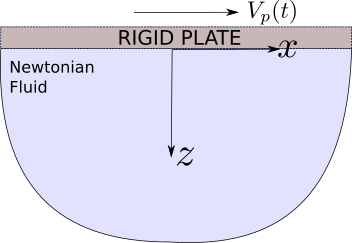
\includegraphics[width=0.8\columnwidth]{bgmodel.png}
\end{column}
\begin{column}{0.6\columnwidth}
\only<2->{If we write down the \textbf{equation of motion} we find
\only<2>{
\[
\rho \frac{\partial v}{\partial t} = \mu \frac{\partial^2 v}{\partial z^2}
\]}
\only<3>{
\[
\rho [ s \tilde{v}(s,z) - v(0,x)] = \mu \frac{d^2 \tilde{v}(s,z)}{dz^2},
\]}
\only<4>{
\[
\tilde{v}(s,z) = \tilde{v}_p(s) \exp\left(\sqrt{\frac{\rho s}{\mu}}z\right)
\]
}\only<5>{
\[
\tilde{\sigma}(s,z) = \sqrt{\mu \rho} \sqrt{s} \tilde{v}(s,z) = \sqrt{\mu \rho} \frac{1}{\sqrt{s}} s \tilde{v}(s,z)
\]
}\only<6>{
\[
\tilde{\sigma}(s,z) = \sqrt{\mu \rho} \mathcal{L} \left\lbrace \frac{1}{\Gamma(\nicefrac{1}{2}) t^{\nicefrac{1}{2}}} \right\rbrace * \mathcal{L}\left\lbrace v_t \right\rbrace
\]
}\only<7>{
\[
\sigma(t,z) = \sqrt{\mu \rho} \frac{1}{\Gamma(\nicefrac{1}{2})} \int_{0}^{t} (t-\tau)^{\nicefrac{1}{2}} v_\tau(\tau,z)\,\textrm{d}\tau.
\]
}\only<8>{
\[
\sigma(t,z) = \sqrt{\mu \rho} {}_{CA}D^{\nicefrac{1}{2}}_{[0,t]} v(t,z).
\]
}\vspace{-1.2em}
\begin{itemize}
	\item<2->$\rho$ is the \emph{fluid density}, $\mu$ is the viscosity, $v$ is
	the profile of the \emph{transverse fluid velocity}. 
	\item<3-> We apply Laplace transform to the equation $\tilde{v} = \mathcal{L}{v}(s)$,
	\item<4-> We solve and impose the boundary condition given by the $\tilde{v}_p = \mathcal{L}{V_p}(s)$,
	\item<5-> Since the \emph{shear stress} is given by $\sigma(t,z) = \mu v_z(t,z)$ we can write its Laplace transform.
	\item<6-> Finally we invert it.
\end{itemize}
	
}
\end{column}
\end{columns}


\end{frame}

\begin{frame}[fragile]{Bagley-Torvik Model~\parencite{BagleyTorvik}}
\begin{columns}
\begin{column}{0.3\columnwidth}
\centering
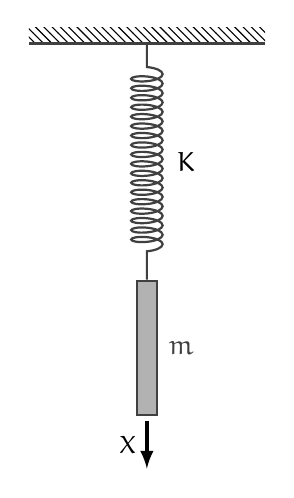
\begin{tikzpicture}[black!75,thick]
% Supporting structure
\fill [pattern = north west lines] (-1.5,0) rectangle ++(3,.2);
\draw[thick] (-1.5,0) -- ++(3,0);
\draw
[
decoration={
	coil,
	aspect=0.3, 
	segment length=1.2mm, 
	amplitude=2mm, 
	pre length=3mm,
	post length=3mm},
decorate
] (0,0) -- ++(0,-3) 
node[midway,right=0.25cm,black]{$K$};
% Mass
\node[draw,
fill=gray!60,
minimum width=0.25cm,
minimum height=1.7cm,
anchor=north,
label=east:$m$] at (0,-3) {};
\draw [very thick,
black,
-latex
] (0,-4.8) -- (0,-5.4) 
node[midway,left]{\small $X$};
\end{tikzpicture}	

Immersed Plate
\end{column}
\begin{column}{0.7\columnwidth}
Assumptions:
\begin{itemize}
	\item The spring is massless and its oscillations do not disturb the fluid,
	\item The area $A$ of the plate is sufficiently large as to produce in the fluid adjacent to
	the plate the velocity field and stresses we just derived,
\end{itemize}
\onslide<2->{
Deriving the equation:
\[
m \ddot{X} = F_X = - K X - 2A \sigma(t,0) 
\]}\onslide<3->{
Using the expression for the \emph{strain} and $V_p(t,0) = \dot{X}(t)$ we find
\[
m \ddot{X}  + 2A \sqrt{\mu \rho} {}_{CA}D^{\nicefrac{3}{2}}_{[0,t]} X + K X = 0.
\]
}
\end{column}
\end{columns}
\end{frame}

\section{Linear Multi-Term FDEs}

\begin{frame}{Linear Multi-Term FDEs}
The Bagley-Torvik model is an example of a \alert{Linear Multi-Term FDE}, that is, something of the form
\[
\lambda_Q {}_{CA}D^{\alpha_Q} y(t) + \lambda_{Q-1}{}_{CA}D^{\alpha_{Q-1}} y(t) + \cdots + \lambda_2 {}_{CA}D^{\alpha_2} y(t) + \lambda_1 {}_{CA}D^{\alpha_1}y(t) = f(t,y(t)),
\]
with 
\begin{itemize}
	\item $\lambda_i \in \mathbb{R}$ $\forall\,i=1,\ldots,Q$,
	\item $0 < \alpha_1 < \alpha_2 < \ldots < \alpha_{Q-1} < \alpha_Q$ and $\alpha_Q \neq 0$.
\end{itemize}
For this problem we have $m_Q = \max m_i$, $m_i = \lceil \alpha_i \rceil$, $i=1,\ldots,Q$ \textbf{initial conditions}:
\begin{equation*}
y(t_0) = y_0, y'(t_0) = y_0^{(1)}, \ldots, y^{(m_Q-1)}(t_0) = y_0^{(m_Q-1)}.
\end{equation*}

\onslide<2>{\faQuestionCircle\, How can we solve them?}

\end{frame}

\begin{frame}{Linear Multi-Term FDEs}
We need to \textbf{recall one of the properties} we have seen of the Caputo derivatives
\begin{itemize}
	\item[$(P_1)$] $I_{[t_0,T]}^\alpha {}_{CA}D_{[t_0,T]}^\alpha y(t) = y(t) - T_{m-1}[y,t_0](t)$,
	\item[$(P_2)$] $I_{[t_0,T]}^\beta {}_{CA}D_{[t_0,T]}^\alpha y(t) = I_{[t_0,T]}^\beta {}_{RL}D_{[t_0,T]}^\alpha \left[ y(t) - T_{m-1}[y;t_0](t) \right] =  I_{[t_0,T]}^{\beta-\alpha}\left[y(t) - T_{m-1}[y;t_0](t)\right]$, $\beta > \alpha$.
\end{itemize}
\onslide<2->{
We start from the multi-term equation
\only<2>{\[
\lambda_Q {}_{CA}D^{\alpha_Q} y(t) + \lambda_{Q-1}{}_{CA}D^{\alpha_{Q-1}} y(t) + \cdots + \lambda_2 {}_{CA}D^{\alpha_2} y(t) + \lambda_1 {}_{CA}D^{\alpha_1}y(t) = f(t,y(t)),
\]}\only<3>{\[
\lambda_Q I_{[t_0,T]}^{\alpha_Q}\left[{}_{CA}D^{\alpha_Q} y(t) \right] = - I_{[t_0,T]}^{\alpha_Q}\left[ \sum_{i=1}^{Q-1} \lambda_i {}_{CA}D^{\alpha_i}y(t) + f(t,y(t))\right],
\]}\only<4>{\[
y(t) - T_{m_Q-1}[y,t_0](t) = - \sum_{i=1}^{Q-1} \frac{\lambda_i}{\lambda_Q} I_{[t_0,t]}^{\alpha_Q - \alpha_i} \left[y(t) - T_{m_i-1}[y;t_0](t) \right] + \frac{1}{\lambda_Q} I_{[t_0,T]}^{\alpha_Q} f(t,y(t))
\]}\only<5>{\[
y(t) = T_{m_Q-1}[y,t_0](t) -\sum_{i=1}^{Q-1} \frac{\lambda_i}{\lambda_Q} I_{[t_0,t]}^{\alpha_Q - \alpha_i} \left[y(t) - T_{m_i-1}[y;t_0](t) \right] + \frac{1}{\lambda_Q} I_{[t_0,T]}^{\alpha_Q} f(t,y(t))
\]}
\begin{itemize}
\item<3-> we multiply both sides by $I_{[t_0,T]}^{\alpha_Q}$,
\item<4-> we use $P_1$ on the left-hand side, $P_2$ on the right-hand side,
\item<5-> and re-arrange to get an expression for the solution.
\end{itemize}
}

\end{frame}

\begin{frame}{Linear Multi-Term FDEs: generalizing PI rules}
First we do a bit of rewriting of
\only<1-2>{\[
y(t) = \alert<2>{T_{m_Q-1}[y,t_0](t) -\sum_{i=1}^{Q-1} \frac{\lambda_i}{\lambda_Q} I_{[t_0,t]}^{\alpha_Q - \alpha_i}} \left[y(t) - \alert<2>{T_{m_i-1}[y;t_0](t)} \right] + \frac{1}{\lambda_Q} I_{[t_0,T]}^{\alpha_Q} f(t,y(t))
\]}\only<3>{\[
y(t) = \tilde{T}(t) - \sum_{i=1}^{Q-1} \frac{\lambda_i}{\lambda_Q} I_{[t_0,t]}^{\alpha_{Q}  - \alpha_i} y(t) + \frac{1}{\lambda_Q} I_{[t_0,T]}^{\alpha_Q} f(t,y(t)).
\]}
\begin{itemize}
	\item<1-> we employ the usual fractional integral for polynomials: \[I_{[t_0,t]}^{\alpha} T_{m-1}[y;t_0](t) = \sum_{k=0}^{m-1} \frac{(t-t_0)^{k+\alpha}}{\Gamma(k+\alpha)} y^{(k)}(t_0), \begin{array}{l} \alpha \in \{\alpha_1,\ldots,\alpha_{Q-1}\}, \\ m \in \{m_1,\ldots,m_{Q-1}\}.\end{array}\]
	\item<2-> We use it to \alert<2>{simplify the expression}
	\[
	\tilde{T}(t) = T_{m_Q-1}[y;t_0](t) + \sum_{i=1}^{Q-1} \frac{\lambda_i}{\lambda_Q} \sum_{k=0}^{m_i-1} \frac{(t-t_0)^{k+\alpha_Q-\alpha_i}}{\Gamma(k+\alpha_Q-\alpha_i+1)}y^{(k)}(t_0).
	\]
\end{itemize}
\end{frame}

\begin{frame}{Linear Multi-Term FDEs: generalizing PI rules}
Now we have an expression that we can treat by adapting one of the Product Integral rules
\[
y(t) = \tilde{T}(t) - \sum_{i=1}^{Q-1} \frac{\lambda_i}{\lambda_Q} I_{[t_0,t]}^{\alpha_{Q}  - \alpha_i} y(t) + \frac{1}{\lambda_Q} I_{[t_0,T]}^{\alpha_Q} f(t,y(t)).
\]
\onslide<2->{
We can start from the \textbf{\only<2>{explicit}\only<3->{implicit} rectangular product integral rule} on a uniform grid
\[
y^{(n)} = \tilde{T}(t_n) - \sum_{i=1}^{Q-1} \frac{\lambda_i}{\lambda_Q} \tau^{\alpha_Q - \alpha_i} \sum_{j=0}^{n\only<2>{-1}} b_{n-j-1}^{(\alpha_Q - \alpha_i)} y^{(j)} + \frac{1}{\lambda_Q} \sum_{j=0}^{n\only<2>{-1}} b_{n-j-1}^{(\alpha_Q)} f(t_j,y^{(j)}). 
\]
with 
\[
b_n^{(\alpha)} = \nicefrac{\displaystyle \left[(n+1)^\alpha - n^\alpha\right]}{\displaystyle \alpha}, \quad n = 1,\ldots,N.
\]
}
\onslide<4>{We can do it similarly for the \textbf{Implicit Trapezoidal Rule} and then for the \textbf{Predictor-Corrector method}~\parencite{DiethelmMultiterm}.}
\end{frame}

\begin{frame}[fragile]{Linear Multi-Term FDEs: generalizing PI rules}

\onslide<1->{\alert{\faQuestionCircle}\; Can we do something similar for FLMMs?}

\onslide<2->{\faCog\;We \alert{don't know} how to determine the starting values $w_{n,j}$ for the quadrature. Thus this approach is not viable.}

\begin{onlyenv}<3>
\small
\textbf{Available codes \parencite{garrappa2018numerical}:}
\begin{itemize}
	\item[\faCode] \verb|MT_FDE_PI1_Ex.m| - \href{https://www.dm.uniba.it/members/garrappa/software_folder/mt_fde_pi1_ex.m}{Explicit Product-Integration of rectanguar type}
	\item[\faCode] \verb|MT_FDE_PI1_Im.m| - \href{https://www.dm.uniba.it/members/garrappa/software_folder/mt_fde_pi1_im.m}{Implicit Product-Integration of rectanguar type}
	\item[\faCode] \verb|MT_FDE_PI2_Im.m| - \href{https://www.dm.uniba.it/members/garrappa/software_folder/mt_fde_pi2_im.m}{Implicit Product-Integration of trapezoidal type}
	\item[\faCode] \verb|MT_FDE_PI12_PC.m|- \href{https://www.dm.uniba.it/members/garrappa/software_folder/mt_fde_pi12_pc.m}{Product-Integration with predictor-corrector}
\end{itemize} 
\end{onlyenv}

\end{frame}

\begin{frame}[fragile]{Linear Multi-Term FDEs: back to Bagley-Torvik}
We reached the equation
\[
m \ddot{X}  + 2A \sqrt{\mu \rho} {}_{CA}D^{\nicefrac{3}{2}}_{[0,t]} X + K X = 0.
\]\vspace{-2em}
\begin{columns}
\begin{column}{0.6\columnwidth}
\definecolor{bg}{rgb}{0.95,0.95,0.95}
\begin{minted}[bgcolor=bg,fontsize=\small,breaklines]{matlab}
m = 10; A = 6; K = 3;
mu = 2; rho = 2;
alpha = [2 3/2] ;
lambda = [m 2*A*sqrt(mu*rho)] ;
f_fun = @(t,X) -K*X;
J_fun = @(t,X) -K;
t0 = 0 ; T = 100 ;
X0 = [0 , 2 ];
h = 1e-2;
[t, X] = mt_fde_pi1_ex(alpha, lambda, f_fun, t0, T, X0, h);
\end{minted}
\end{column}
\begin{column}{0.4\columnwidth}
\centering

% This file was created by matlab2tikz.
%
%The latest updates can be retrieved from
%  http://www.mathworks.com/matlabcentral/fileexchange/22022-matlab2tikz-matlab2tikz
%where you can also make suggestions and rate matlab2tikz.
%
\definecolor{mycolor1}{rgb}{0.00000,0.44700,0.74100}%
%
\begin{tikzpicture}

\begin{axis}[%
width=0.9\columnwidth,
height=1.5in,
at={(0.772in,0.481in)},
scale only axis,
xmin=0,
xmax=100,
ymin=0,
ymax=8,
axis background/.style={fill=white}
]
\addplot [color=mycolor1, line width=2.0pt, forget plot]
  table[row sep=crcr]{%
0	0\\
0.01	0.0236108133347056\\
0.02	0.0438185002436616\\
0.03	0.0642455751460625\\
0.04	0.0845358405025254\\
0.05	0.104775392332668\\
0.06	0.124973976833812\\
0.07	0.145142198726337\\
0.08	0.165286117268426\\
0.09	0.185409873976864\\
0.1	0.205516340036638\\
0.11	0.225607573940143\\
0.12	0.245685081621196\\
0.13	0.265749981327451\\
0.14	0.285803111218886\\
0.15	0.305845102231272\\
0.16	0.325876428852595\\
0.17	0.345897445403013\\
0.18	0.365908412520664\\
0.19	0.385909516863987\\
0.2	0.405900886012114\\
0.21	0.425882599899867\\
0.22	0.445854699708607\\
0.23	0.465817194860368\\
0.24	0.485770068578207\\
0.25	0.505713282349084\\
0.26	0.52564677953705\\
0.27	0.545570488331706\\
0.28	0.56548432417166\\
0.29	0.585388191749682\\
0.3	0.605281986681869\\
0.31	0.625165596904899\\
0.32	0.645038903851735\\
0.33	0.6649017834456\\
0.34	0.684754106944022\\
0.35	0.704595741658485\\
0.36	0.724426551570317\\
0.37	0.744246397859615\\
0.38	0.76405513936094\\
0.39	0.783852632957089\\
0.4	0.80363873392028\\
0.41	0.823413296208521\\
0.42	0.843176172723641\\
0.43	0.862927215536403\\
0.44	0.882666276083295\\
0.45	0.90239320533883\\
0.46	0.922107853966659\\
0.47	0.941810072452259\\
0.48	0.961499711219597\\
0.49	0.981176620733799\\
0.5	1.00084065159157\\
0.51	1.0204916546009\\
0.52	1.04012948085128\\
0.53	1.05975398177574\\
0.54	1.07936500920542\\
0.55	1.09896241541776\\
0.56	1.11854605317901\\
0.57	1.13811577578154\\
0.58	1.15767143707677\\
0.59	1.17721289150408\\
0.6	1.19673999411612\\
0.61	1.21625260060097\\
0.62	1.23575056730154\\
0.63	1.25523375123235\\
0.64	1.27470201009412\\
0.65	1.29415520228634\\
0.66	1.31359318691806\\
0.67	1.33301582381699\\
0.68	1.35242297353725\\
0.69	1.37181449736578\\
0.7	1.39119025732758\\
0.71	1.41055011618995\\
0.72	1.42989393746575\\
0.73	1.44922158541586\\
0.74	1.4685329250509\\
0.75	1.48782782213219\\
0.76	1.50710614317223\\
0.77	1.52636775543457\\
0.78	1.54561252693319\\
0.79	1.56484032643145\\
0.8	1.58405102344071\\
0.81	1.60324448821852\\
0.82	1.62242059176654\\
0.83	1.64157920582822\\
0.84	1.66072020288616\\
0.85	1.67984345615933\\
0.86	1.69894883960001\\
0.87	1.71803622789066\\
0.88	1.73710549644058\\
0.89	1.75615652138243\\
0.9	1.77518917956869\\
0.91	1.79420334856797\\
0.92	1.81319890666125\\
0.93	1.83217573283807\\
0.94	1.85113370679263\\
0.95	1.87007270891984\\
0.96	1.88899262031137\\
0.97	1.90789332275162\\
0.98	1.92677469871366\\
0.99	1.9456366313552\\
1	1.96447900451451\\
1.01	1.98330170270633\\
1.02	2.00210461111782\\
1.03	2.02088761560445\\
1.04	2.03965060268596\\
1.05	2.05839345954229\\
1.06	2.0771160740095\\
1.07	2.09581833457582\\
1.08	2.11450013037758\\
1.09	2.13316135119522\\
1.1	2.15180188744938\\
1.11	2.17042163019693\\
1.12	2.18902047112705\\
1.13	2.20759830255738\\
1.14	2.22615501743017\\
1.15	2.24469050930843\\
1.16	2.2632046723722\\
1.17	2.28169740141477\\
1.18	2.30016859183893\\
1.19	2.31861813965339\\
1.2	2.33704594146901\\
1.21	2.35545189449531\\
1.22	2.3738358965368\\
1.23	2.3921978459895\\
1.24	2.41053764183744\\
1.25	2.42885518364917\\
1.26	2.44715037157436\\
1.27	2.46542310634039\\
1.28	2.48367328924901\\
1.29	2.50190082217305\\
1.3	2.52010560755307\\
1.31	2.53828754839421\\
1.32	2.55644654826292\\
1.33	2.57458251128382\\
1.34	2.59269534213653\\
1.35	2.61078494605263\\
1.36	2.62885122881255\\
1.37	2.64689409674259\\
1.38	2.66491345671185\\
1.39	2.68290921612935\\
1.4	2.70088128294107\\
1.41	2.71882956562706\\
1.42	2.7367539731986\\
1.43	2.75465441519533\\
1.44	2.77253080168254\\
1.45	2.79038304324831\\
1.46	2.80821105100086\\
1.47	2.82601473656584\\
1.48	2.84379401208361\\
1.49	2.86154879020668\\
1.5	2.87927898409705\\
1.51	2.89698450742366\\
1.52	2.91466527435984\\
1.53	2.9323211995808\\
1.54	2.94995219826113\\
1.55	2.96755818607232\\
1.56	2.98513907918038\\
1.57	3.0026947942434\\
1.58	3.02022524840915\\
1.59	3.03773035931278\\
1.6	3.05521004507447\\
1.61	3.07266422429712\\
1.62	3.09009281606407\\
1.63	3.1074957399369\\
1.64	3.12487291595314\\
1.65	3.1422242646241\\
1.66	3.15954970693271\\
1.67	3.17684916433134\\
1.68	3.19412255873967\\
1.69	3.2113698125426\\
1.7	3.22859084858816\\
1.71	3.24578559018544\\
1.72	3.26295396110254\\
1.73	3.28009588556459\\
1.74	3.29721128825171\\
1.75	3.31430009429704\\
1.76	3.33136222928481\\
1.77	3.34839761924836\\
1.78	3.36540619066826\\
1.79	3.38238787047041\\
1.8	3.39934258602413\\
1.81	3.41627026514033\\
1.82	3.43317083606966\\
1.83	3.45004422750068\\
1.84	3.46689036855809\\
1.85	3.48370918880088\\
1.86	3.50050061822061\\
1.87	3.51726458723967\\
1.88	3.53400102670949\\
1.89	3.55070986790886\\
1.9	3.56739104254224\\
1.91	3.58404448273803\\
1.92	3.60067012104693\\
1.93	3.6172678904403\\
1.94	3.63383772430848\\
1.95	3.6503795564592\\
1.96	3.66689332111597\\
1.97	3.68337895291646\\
1.98	3.69983638691094\\
1.99	3.71626555856075\\
2	3.73266640373664\\
2.01	3.7490388587174\\
2.02	3.76538286018815\\
2.03	3.78169834523898\\
2.04	3.79798525136338\\
2.05	3.81424351645679\\
2.06	3.83047307881509\\
2.07	3.84667387713316\\
2.08	3.86284585050346\\
2.09	3.87898893841456\\
2.1	3.89510308074975\\
2.11	3.91118821778559\\
2.12	3.92724429019056\\
2.13	3.94327123902362\\
2.14	3.95926900573292\\
2.15	3.97523753215431\\
2.16	3.99117676051014\\
2.17	4.00708663340775\\
2.18	4.02296709383831\\
2.19	4.03881808517536\\
2.2	4.05463955117358\\
2.21	4.07043143596745\\
2.22	4.08619368407\\
2.23	4.10192624037149\\
2.24	4.11762905013815\\
2.25	4.13330205901096\\
2.26	4.14894521300431\\
2.27	4.16455845850486\\
2.28	4.18014174227025\\
2.29	4.19569501142787\\
2.3	4.2112182134737\\
2.31	4.22671129627101\\
2.32	4.24217420804929\\
2.33	4.25760689740294\\
2.34	4.27300931329014\\
2.35	4.28838140503176\\
2.36	4.30372312231001\\
2.37	4.31903441516748\\
2.38	4.33431523400584\\
2.39	4.34956552958484\\
2.4	4.36478525302101\\
2.41	4.37997435578673\\
2.42	4.39513278970896\\
2.43	4.41026050696818\\
2.44	4.42535746009732\\
2.45	4.44042360198064\\
2.46	4.45545888585263\\
2.47	4.47046326529694\\
2.48	4.48543669424532\\
2.49	4.50037912697655\\
2.5	4.51529051811535\\
2.51	4.53017082263138\\
2.52	4.54501999583812\\
2.53	4.55983799339191\\
2.54	4.57462477129088\\
2.55	4.5893802858739\\
2.56	4.6041044938196\\
2.57	4.61879735214531\\
2.58	4.63345881820612\\
2.59	4.64808884969379\\
2.6	4.66268740463583\\
2.61	4.67725444139443\\
2.62	4.69178991866558\\
2.63	4.70629379547798\\
2.64	4.72076603119212\\
2.65	4.73520658549934\\
2.66	4.74961541842079\\
2.67	4.76399249030651\\
2.68	4.77833776183454\\
2.69	4.79265119400983\\
2.7	4.80693274816343\\
2.71	4.82118238595151\\
2.72	4.83540006935436\\
2.73	4.84958576067558\\
2.74	4.86373942254107\\
2.75	4.87786101789814\\
2.76	4.89195051001459\\
2.77	4.90600786247783\\
2.78	4.92003303919394\\
2.79	4.93402600438677\\
2.8	4.94798672259707\\
2.81	4.96191515868158\\
2.82	4.97581127781217\\
2.83	4.98967504547493\\
2.84	5.00350642746927\\
2.85	5.01730538990714\\
2.86	5.03107189921204\\
2.87	5.04480592211825\\
2.88	5.0585074256699\\
2.89	5.07217637722017\\
2.9	5.08581274443041\\
2.91	5.09941649526929\\
2.92	5.11298759801195\\
2.93	5.12652602123916\\
2.94	5.14003173383651\\
2.95	5.15350470499353\\
2.96	5.16694490420289\\
2.97	5.18035230125959\\
2.98	5.19372686626004\\
2.99	5.20706856960142\\
3	5.22037738198066\\
3.01	5.23365327439378\\
3.02	5.24689621813499\\
3.03	5.26010618479596\\
3.04	5.27328314626493\\
3.05	5.28642707472597\\
3.06	5.29953794265818\\
3.07	5.3126157228349\\
3.08	5.32566038832285\\
3.09	5.33867191248147\\
3.1	5.35165026896202\\
3.11	5.36459543170686\\
3.12	5.37750737494866\\
3.13	5.39038607320962\\
3.14	5.4032315013007\\
3.15	5.41604363432085\\
3.16	5.42882244765625\\
3.17	5.44156791697956\\
3.18	5.45428001824912\\
3.19	5.46695872770822\\
3.2	5.47960402188438\\
3.21	5.49221587758848\\
3.22	5.50479427191418\\
3.23	5.51733918223702\\
3.24	5.52985058621377\\
3.25	5.54232846178163\\
3.26	5.55477278715757\\
3.27	5.56718354083749\\
3.28	5.57956070159556\\
3.29	5.59190424848349\\
3.3	5.60421416082974\\
3.31	5.61649041823884\\
3.32	5.62873300059071\\
3.33	5.64094188803978\\
3.34	5.65311706101449\\
3.35	5.66525850021641\\
3.36	5.67736618661954\\
3.37	5.6894401014697\\
3.38	5.7014802262837\\
3.39	5.71348654284871\\
3.4	5.72545903322152\\
3.41	5.73739767972785\\
3.42	5.74930246496162\\
3.43	5.76117337178431\\
3.44	5.77301038332418\\
3.45	5.78481348297568\\
3.46	5.79658265439862\\
3.47	5.80831788151763\\
3.48	5.82001914852134\\
3.49	5.83168643986178\\
3.5	5.84331974025365\\
3.51	5.85491903467365\\
3.52	5.8664843083598\\
3.53	5.87801554681078\\
3.54	5.88951273578517\\
3.55	5.90097586130092\\
3.56	5.91240490963452\\
3.57	5.92379986732042\\
3.58	5.93516072115034\\
3.59	5.94648745817264\\
3.6	5.95778006569152\\
3.61	5.96903853126655\\
3.62	5.98026284271182\\
3.63	5.99145298809542\\
3.64	6.00260895573868\\
3.65	6.01373073421562\\
3.66	6.02481831235211\\
3.67	6.03587167922545\\
3.68	6.04689082416356\\
3.69	6.05787573674433\\
3.7	6.06882640679506\\
3.71	6.07974282439172\\
3.72	6.09062497985836\\
3.73	6.10147286376643\\
3.74	6.1122864669342\\
3.75	6.12306578042598\\
3.76	6.13381079555167\\
3.77	6.14452150386592\\
3.78	6.15519789716769\\
3.79	6.16583996749941\\
3.8	6.17644770714655\\
3.81	6.18702110863681\\
3.82	6.19756016473961\\
3.83	6.20806486846536\\
3.84	6.21853521306494\\
3.85	6.22897119202901\\
3.86	6.23937279908732\\
3.87	6.24974002820825\\
3.88	6.260072873598\\
3.89	6.2703713297001\\
3.9	6.28063539119476\\
3.91	6.2908650529982\\
3.92	6.30106031026208\\
3.93	6.31122115837286\\
3.94	6.32134759295121\\
3.95	6.33143960985136\\
3.96	6.3414972051605\\
3.97	6.3515203751982\\
3.98	6.36150911651572\\
3.99	6.37146342589551\\
4	6.38138330035047\\
4.01	6.39126873712347\\
4.02	6.40111973368666\\
4.03	6.4109362877409\\
4.04	6.42071839721513\\
4.05	6.43046606026581\\
4.06	6.44017927527628\\
4.07	6.44985804085612\\
4.08	6.45950235584072\\
4.09	6.46911221929044\\
4.1	6.47868763049019\\
4.11	6.48822858894882\\
4.12	6.49773509439839\\
4.13	6.50720714679373\\
4.14	6.51664474631177\\
4.15	6.526047893351\\
4.16	6.53541658853076\\
4.17	6.54475083269081\\
4.18	6.55405062689064\\
4.19	6.56331597240893\\
4.2	6.57254687074286\\
4.21	6.58174332360771\\
4.22	6.59090533293607\\
4.23	6.60003290087744\\
4.24	6.6091260297975\\
4.25	6.61818472227761\\
4.26	6.62720898111425\\
4.27	6.63619880931834\\
4.28	6.6451542101147\\
4.29	6.6540751869416\\
4.3	6.66296174344997\\
4.31	6.67181388350299\\
4.32	6.68063161117542\\
4.33	6.68941493075305\\
4.34	6.69816384673219\\
4.35	6.70687836381898\\
4.36	6.71555848692891\\
4.37	6.72420422118624\\
4.38	6.73281557192335\\
4.39	6.74139254468033\\
4.4	6.74993514520421\\
4.41	6.75844337944855\\
4.42	6.76691725357282\\
4.43	6.77535677394181\\
4.44	6.78376194712513\\
4.45	6.79213277989656\\
4.46	6.80046927923354\\
4.47	6.80877145231667\\
4.48	6.81703930652897\\
4.49	6.82527284945549\\
4.5	6.8334720888827\\
4.51	6.84163703279789\\
4.52	6.84976768938867\\
4.53	6.85786406704236\\
4.54	6.86592617434546\\
4.55	6.87395402008308\\
4.56	6.88194761323848\\
4.57	6.8899069629923\\
4.58	6.89783207872228\\
4.59	6.90572297000246\\
4.6	6.91357964660279\\
4.61	6.92140211848848\\
4.62	6.92919039581958\\
4.63	6.93694448895025\\
4.64	6.94466440842838\\
4.65	6.95235016499491\\
4.66	6.96000176958338\\
4.67	6.96761923331934\\
4.68	6.97520256751978\\
4.69	6.98275178369266\\
4.7	6.99026689353627\\
4.71	6.99774790893879\\
4.72	7.00519484197764\\
4.73	7.01260770491903\\
4.74	7.01998651021735\\
4.75	7.02733127051467\\
4.76	7.03464199864021\\
4.77	7.04191870760974\\
4.78	7.0491614106251\\
4.79	7.05637012107363\\
4.8	7.06354485252771\\
4.81	7.07068561874406\\
4.82	7.07779243366333\\
4.83	7.08486531140959\\
4.84	7.09190426628969\\
4.85	7.09890931279281\\
4.86	7.10588046558985\\
4.87	7.11281773953299\\
4.88	7.11972114965508\\
4.89	7.12659071116917\\
4.9	7.13342643946795\\
4.91	7.14022835012313\\
4.92	7.14699645888514\\
4.93	7.15373078168233\\
4.94	7.16043133462069\\
4.95	7.16709813398309\\
4.96	7.17373119622897\\
4.97	7.18033053799364\\
4.98	7.18689617608787\\
4.99	7.19342812749728\\
5	7.19992640938194\\
5.01	7.20639103907565\\
5.02	7.21282203408561\\
5.03	7.2192194120918\\
5.04	7.22558319094644\\
5.05	7.23191338867362\\
5.06	7.23821002346852\\
5.07	7.2444731136971\\
5.08	7.25070267789557\\
5.09	7.25689873476968\\
5.1	7.26306130319451\\
5.11	7.26919040221364\\
5.12	7.27528605103884\\
5.13	7.28134826904947\\
5.14	7.28737707579202\\
5.15	7.29337249097952\\
5.16	7.29933453449105\\
5.17	7.30526322637126\\
5.18	7.31115858682985\\
5.19	7.31702063624103\\
5.2	7.32284939514301\\
5.21	7.32864488423751\\
5.22	7.33440712438926\\
5.23	7.34013613662539\\
5.24	7.34583194213509\\
5.25	7.35149456226896\\
5.26	7.35712401853858\\
5.27	7.36272033261592\\
5.28	7.3682835263329\\
5.29	7.37381362168096\\
5.3	7.3793106408103\\
5.31	7.38477460602968\\
5.32	7.39020553980564\\
5.33	7.39560346476226\\
5.34	7.40096840368038\\
5.35	7.40630037949739\\
5.36	7.41159941530641\\
5.37	7.41686553435607\\
5.38	7.42209876004985\\
5.39	7.42729911594563\\
5.4	7.43246662575516\\
5.41	7.43760131334354\\
5.42	7.44270320272884\\
5.43	7.44777231808143\\
5.44	7.45280868372372\\
5.45	7.45781232412926\\
5.46	7.46278326392274\\
5.47	7.46772152787909\\
5.48	7.47262714092324\\
5.49	7.47750012812942\\
5.5	7.48234051472084\\
5.51	7.48714832606909\\
5.52	7.49192358769376\\
5.53	7.49666632526172\\
5.54	7.5013765645869\\
5.55	7.50605433162958\\
5.56	7.51069965249607\\
5.57	7.51531255343805\\
5.58	7.51989306085219\\
5.59	7.5244412012797\\
5.6	7.52895700140569\\
5.61	7.53344048805878\\
5.62	7.53789168821062\\
5.63	7.54231062897538\\
5.64	7.54669733760919\\
5.65	7.55105184150983\\
5.66	7.55537416821604\\
5.67	7.55966434540714\\
5.68	7.56392240090261\\
5.69	7.56814836266142\\
5.7	7.5723422587817\\
5.71	7.57650411750022\\
5.72	7.58063396719189\\
5.73	7.58473183636924\\
5.74	7.58879775368202\\
5.75	7.59283174791663\\
5.76	7.59683384799575\\
5.77	7.60080408297771\\
5.78	7.60474248205619\\
5.79	7.60864907455953\\
5.8	7.61252388995044\\
5.81	7.61636695782543\\
5.82	7.6201783079143\\
5.83	7.62395797007975\\
5.84	7.62770597431682\\
5.85	7.63142235075253\\
5.86	7.63510712964522\\
5.87	7.63876034138424\\
5.88	7.64238201648937\\
5.89	7.64597218561047\\
5.9	7.64953087952684\\
5.91	7.65305812914684\\
5.92	7.65655396550741\\
5.93	7.66001841977369\\
5.94	7.66345152323829\\
5.95	7.66685330732105\\
5.96	7.67022380356852\\
5.97	7.67356304365345\\
5.98	7.67687105937434\\
5.99	7.6801478826549\\
6	7.68339354554375\\
6.01	7.68660808021381\\
6.02	7.68979151896181\\
6.03	7.69294389420795\\
6.04	7.69606523849533\\
6.05	7.69915558448955\\
6.06	7.70221496497818\\
6.07	7.70524341287027\\
6.08	7.70824096119611\\
6.09	7.71120764310639\\
6.1	7.71414349187211\\
6.11	7.71704854088378\\
6.12	7.71992282365127\\
6.13	7.72276637380315\\
6.14	7.72557922508625\\
6.15	7.72836141136523\\
6.16	7.73111296662212\\
6.17	7.73383392495591\\
6.18	7.73652432058193\\
6.19	7.73918418783161\\
6.2	7.74181356115182\\
6.21	7.74441247510445\\
6.22	7.74698096436619\\
6.23	7.74951906372764\\
6.24	7.75202680809327\\
6.25	7.75450423248071\\
6.26	7.75695137202037\\
6.27	7.75936826195506\\
6.28	7.76175493763925\\
6.29	7.76411143453913\\
6.3	7.76643778823155\\
6.31	7.76873403440409\\
6.32	7.77100020885428\\
6.33	7.77323634748924\\
6.34	7.77544248632526\\
6.35	7.77761866148738\\
6.36	7.77976490920874\\
6.37	7.78188126583044\\
6.38	7.78396776780085\\
6.39	7.78602445167517\\
6.4	7.78805135411518\\
6.41	7.79004851188856\\
6.42	7.79201596186856\\
6.43	7.79395374103352\\
6.44	7.79586188646648\\
6.45	7.79774043535463\\
6.46	7.79958942498898\\
6.47	7.80140889276376\\
6.48	7.80319887617621\\
6.49	7.80495941282586\\
6.5	7.80669054041428\\
6.51	7.80839229674461\\
6.52	7.81006471972103\\
6.53	7.8117078473484\\
6.54	7.81332171773179\\
6.55	7.81490636907598\\
6.56	7.81646183968523\\
6.57	7.8179881679625\\
6.58	7.81948539240932\\
6.59	7.82095355162522\\
6.6	7.82239268430725\\
6.61	7.82380282924958\\
6.62	7.82518402534313\\
6.63	7.8265363115751\\
6.64	7.82785972702837\\
6.65	7.82915431088135\\
6.66	7.83042010240728\\
6.67	7.83165714097404\\
6.68	7.83286546604348\\
6.69	7.83404511717109\\
6.7	7.83519613400566\\
6.71	7.83631855628862\\
6.72	7.83741242385388\\
6.73	7.83847777662719\\
6.74	7.83951465462571\\
6.75	7.8405230979578\\
6.76	7.84150314682228\\
6.77	7.84245484150828\\
6.78	7.84337822239463\\
6.79	7.84427332994944\\
6.8	7.84514020472979\\
6.81	7.84597888738123\\
6.82	7.84678941863729\\
6.83	7.84757183931916\\
6.84	7.84832619033515\\
6.85	7.84905251268047\\
6.86	7.84975084743655\\
6.87	7.85042123577071\\
6.88	7.85106371893587\\
6.89	7.85167833826994\\
6.9	7.85226513519547\\
6.91	7.85282415121923\\
6.92	7.85335542793173\\
6.93	7.85385900700702\\
6.94	7.85433493020194\\
6.95	7.85478323935587\\
6.96	7.8552039763903\\
6.97	7.85559718330854\\
6.98	7.85596290219502\\
6.99	7.85630117521506\\
7	7.85661204461446\\
7.01	7.85689555271894\\
7.02	7.85715174193392\\
7.03	7.85738065474388\\
7.04	7.85758233371222\\
7.05	7.85775682148052\\
7.06	7.85790416076848\\
7.07	7.85802439437311\\
7.08	7.85811756516869\\
7.09	7.85818371610608\\
7.1	7.85822289021253\\
7.11	7.85823513059101\\
7.12	7.85822048042007\\
7.13	7.85817898295328\\
7.14	7.85811068151873\\
7.15	7.85801561951891\\
7.16	7.85789384042994\\
7.17	7.85774538780147\\
7.18	7.8575703052561\\
7.19	7.85736863648899\\
7.2	7.8571404252675\\
7.21	7.85688571543074\\
7.22	7.85660455088921\\
7.23	7.85629697562439\\
7.24	7.85596303368819\\
7.25	7.85560276920281\\
7.26	7.8552162263601\\
7.27	7.85480344942128\\
7.28	7.85436448271647\\
7.29	7.85389937064437\\
7.3	7.85340815767179\\
7.31	7.85289088833325\\
7.32	7.85234760723053\\
7.33	7.85177835903254\\
7.34	7.85118318847447\\
7.35	7.85056214035775\\
7.36	7.8499152595496\\
7.37	7.84924259098238\\
7.38	7.84854417965361\\
7.39	7.8478200706251\\
7.4	7.84707030902297\\
7.41	7.84629494003697\\
7.42	7.84549400892028\\
7.43	7.84466756098893\\
7.44	7.84381564162161\\
7.45	7.84293829625907\\
7.46	7.84203557040382\\
7.47	7.84110750961977\\
7.48	7.84015415953191\\
7.49	7.8391755658256\\
7.5	7.83817177424655\\
7.51	7.83714283060018\\
7.52	7.83608878075145\\
7.53	7.83500967062413\\
7.54	7.8339055462008\\
7.55	7.83277645352224\\
7.56	7.8316224386871\\
7.57	7.83044354785132\\
7.58	7.82923982722821\\
7.59	7.82801132308754\\
7.6	7.82675808175545\\
7.61	7.8254801496141\\
7.62	7.82417757310103\\
7.63	7.82285039870898\\
7.64	7.82149867298554\\
7.65	7.82012244253258\\
7.66	7.81872175400598\\
7.67	7.81729665411527\\
7.68	7.8158471896233\\
7.69	7.81437340734556\\
7.7	7.81287535415017\\
7.71	7.81135307695732\\
7.72	7.80980662273892\\
7.73	7.80823603851813\\
7.74	7.80664137136927\\
7.75	7.8050226684169\\
7.76	7.80337997683612\\
7.77	7.80171334385177\\
7.78	7.80002281673792\\
7.79	7.79830844281796\\
7.8	7.79657026946391\\
7.81	7.79480834409609\\
7.82	7.7930227141827\\
7.83	7.79121342723964\\
7.84	7.78938053082998\\
7.85	7.78752407256364\\
7.86	7.78564410009685\\
7.87	7.78374066113207\\
7.88	7.78181380341751\\
7.89	7.77986357474661\\
7.9	7.77789002295778\\
7.91	7.77589319593416\\
7.92	7.77387314160305\\
7.93	7.7718299079356\\
7.94	7.76976354294656\\
7.95	7.76767409469367\\
7.96	7.76556161127761\\
7.97	7.76342614084128\\
7.98	7.76126773156983\\
7.99	7.75908643168989\\
8	7.75688228946954\\
8.01	7.75465535321769\\
8.02	7.75240567128398\\
8.03	7.75013329205817\\
8.04	7.74783826396993\\
8.05	7.74552063548833\\
8.06	7.74318045512172\\
8.07	7.74081777141718\\
8.08	7.73843263296018\\
8.09	7.73602508837422\\
8.1	7.73359518632076\\
8.11	7.73114297549814\\
8.12	7.72866850464216\\
8.13	7.72617182252495\\
8.14	7.72365297795498\\
8.15	7.72111201977676\\
8.16	7.71854899687031\\
8.17	7.71596395815072\\
8.18	7.71335695256814\\
8.19	7.71072802910712\\
8.2	7.70807723678643\\
8.21	7.7054046246585\\
8.22	7.70271024180939\\
8.23	7.69999413735815\\
8.24	7.69725636045658\\
8.25	7.69449696028893\\
8.26	7.69171598607149\\
8.27	7.68891348705221\\
8.28	7.68608951251046\\
8.29	7.68324411175654\\
8.3	7.68037733413147\\
8.31	7.67748922900657\\
8.32	7.67457984578311\\
8.33	7.67164923389196\\
8.34	7.66869744279337\\
8.35	7.66572452197643\\
8.36	7.66273052095882\\
8.37	7.65971548928653\\
8.38	7.65667947653346\\
8.39	7.65362253230099\\
8.4	7.65054470621777\\
8.41	7.64744604793938\\
8.42	7.64432660714792\\
8.43	7.64118643355157\\
8.44	7.63802557688462\\
8.45	7.63484408690667\\
8.46	7.63164201340266\\
8.47	7.62841940618225\\
8.48	7.62517631507976\\
8.49	7.62191278995352\\
8.5	7.61862888068595\\
8.51	7.61532463718267\\
8.52	7.61200010937277\\
8.53	7.60865534720801\\
8.54	7.60529040066281\\
8.55	7.60190531973349\\
8.56	7.59850015443863\\
8.57	7.59507495481787\\
8.58	7.5916297709324\\
8.59	7.58816465286414\\
8.6	7.58467965071551\\
8.61	7.58117481460915\\
8.62	7.57765019468759\\
8.63	7.57410584111285\\
8.64	7.5705418040662\\
8.65	7.56695813374786\\
8.66	7.56335488037652\\
8.67	7.55973209418917\\
8.68	7.55608982544069\\
8.69	7.55242812440353\\
8.7	7.5487470413675\\
8.71	7.54504662663919\\
8.72	7.54132693054198\\
8.73	7.53758800341546\\
8.74	7.53382989561521\\
8.75	7.53005265751249\\
8.76	7.52625633949394\\
8.77	7.52244099196109\\
8.78	7.51860666533036\\
8.79	7.51475341003236\\
8.8	7.51088127651187\\
8.81	7.50699031522741\\
8.82	7.50308057665097\\
8.83	7.49915211126758\\
8.84	7.49520496957509\\
8.85	7.49123920208388\\
8.86	7.48725485931652\\
8.87	7.48325199180736\\
8.88	7.47923065010237\\
8.89	7.47519088475868\\
8.9	7.47113274634444\\
8.91	7.46705628543837\\
8.92	7.4629615526295\\
8.93	7.45884859851676\\
8.94	7.45471747370901\\
8.95	7.45056822882422\\
8.96	7.44640091448949\\
8.97	7.44221558134083\\
8.98	7.4380122800226\\
8.99	7.43379106118729\\
9	7.42955197549517\\
9.01	7.42529507361425\\
9.02	7.42102040621965\\
9.03	7.4167280239933\\
9.04	7.4124179776241\\
9.05	7.40809031780686\\
9.06	7.40374509524266\\
9.07	7.39938236063836\\
9.08	7.39500216470596\\
9.09	7.39060455816293\\
9.1	7.38618959173127\\
9.11	7.38175731613764\\
9.12	7.37730778211296\\
9.13	7.3728410403919\\
9.14	7.36835714171299\\
9.15	7.36385613681793\\
9.16	7.35933807645149\\
9.17	7.35480301136119\\
9.18	7.35025099229711\\
9.19	7.34568207001116\\
9.2	7.34109629525769\\
9.21	7.3364937187918\\
9.22	7.33187439137061\\
9.23	7.32723836375193\\
9.24	7.32258568669412\\
9.25	7.31791641095616\\
9.26	7.31323058729703\\
9.27	7.30852826647561\\
9.28	7.30380949925024\\
9.29	7.29907433637852\\
9.3	7.29432282861704\\
9.31	7.28955502672102\\
9.32	7.28477098144408\\
9.33	7.27997074353793\\
9.34	7.27515436375222\\
9.35	7.27032189283387\\
9.36	7.26547338152726\\
9.37	7.26060888057371\\
9.38	7.25572844071107\\
9.39	7.25083211267375\\
9.4	7.24591994719223\\
9.41	7.24099199499282\\
9.42	7.23604830679734\\
9.43	7.23108893332299\\
9.44	7.22611392528181\\
9.45	7.22112333338079\\
9.46	7.21611720832111\\
9.47	7.21109560079829\\
9.48	7.20605856150159\\
9.49	7.2010061411141\\
9.5	7.19593839031198\\
9.51	7.19085535976475\\
9.52	7.18575710013446\\
9.53	7.18064366207568\\
9.54	7.17551509623545\\
9.55	7.17037145325258\\
9.56	7.16521278375765\\
9.57	7.16003913837265\\
9.58	7.15485056771068\\
9.59	7.14964712237584\\
9.6	7.14442885296273\\
9.61	7.13919581005642\\
9.62	7.13394804423194\\
9.63	7.12868560605423\\
9.64	7.12340854607763\\
9.65	7.11811691484593\\
9.66	7.11281076289183\\
9.67	7.10749014073687\\
9.68	7.10215509889096\\
9.69	7.09680568785234\\
9.7	7.09144195810713\\
9.71	7.08606396012912\\
9.72	7.08067174437971\\
9.73	7.07526536130717\\
9.74	7.06984486134708\\
9.75	7.06441029492125\\
9.76	7.05896171243828\\
9.77	7.0534991642925\\
9.78	7.04802270086448\\
9.79	7.0425323725203\\
9.8	7.03702822961111\\
9.81	7.03151032247365\\
9.82	7.02597870142917\\
9.83	7.02043341678356\\
9.84	7.01487451882717\\
9.85	7.00930205783436\\
9.86	7.0037160840633\\
9.87	6.99811664775581\\
9.88	6.99250379913693\\
9.89	6.98687758841487\\
9.9	6.9812380657806\\
9.91	6.97558528140766\\
9.92	6.96991928545209\\
9.93	6.96424012805178\\
9.94	6.95854785932646\\
9.95	6.95284252937762\\
9.96	6.94712418828786\\
9.97	6.94139288612109\\
9.98	6.93564867292187\\
9.99	6.92989159871544\\
10	6.92412171350742\\
10.01	6.91833906728345\\
10.02	6.912543710009\\
10.03	6.90673569162941\\
10.04	6.90091506206906\\
10.05	6.89508187123172\\
10.06	6.88923616899987\\
10.07	6.88337800523472\\
10.08	6.87750742977599\\
10.09	6.87162449244138\\
10.1	6.86572924302672\\
10.11	6.8598217313054\\
10.12	6.85390200702828\\
10.13	6.84797011992349\\
10.14	6.84202611969619\\
10.15	6.83607005602811\\
10.16	6.83010197857767\\
10.17	6.82412193697952\\
10.18	6.81812998084436\\
10.19	6.81212615975869\\
10.2	6.80611052328464\\
10.21	6.80008312095953\\
10.22	6.79404400229598\\
10.23	6.78799321678142\\
10.24	6.78193081387789\\
10.25	6.77585684302205\\
10.26	6.76977135362461\\
10.27	6.76367439507008\\
10.28	6.75756601671711\\
10.29	6.75144626789751\\
10.3	6.7453151979166\\
10.31	6.7391728560526\\
10.32	6.7330192915568\\
10.33	6.72685455365267\\
10.34	6.72067869153665\\
10.35	6.71449175437689\\
10.36	6.70829379131368\\
10.37	6.70208485145909\\
10.38	6.69586498389643\\
10.39	6.68963423768041\\
10.4	6.68339266183717\\
10.41	6.67714030536287\\
10.42	6.67087721722504\\
10.43	6.66460344636148\\
10.44	6.65831904167976\\
10.45	6.6520240520578\\
10.46	6.64571852634313\\
10.47	6.63940251335303\\
10.48	6.63307606187361\\
10.49	6.6267392206605\\
10.5	6.6203920384382\\
10.51	6.61403456389954\\
10.52	6.60766684570633\\
10.53	6.60128893248807\\
10.54	6.59490087284283\\
10.55	6.58850271533601\\
10.56	6.58209450850103\\
10.57	6.57567630083841\\
10.58	6.56924814081609\\
10.59	6.5628100768689\\
10.6	6.55636215739845\\
10.61	6.54990443077286\\
10.62	6.54343694532669\\
10.63	6.53695974936069\\
10.64	6.53047289114146\\
10.65	6.52397641890147\\
10.66	6.51747038083859\\
10.67	6.51095482511602\\
10.68	6.50442979986239\\
10.69	6.49789535317082\\
10.7	6.49135153309945\\
10.71	6.48479838767084\\
10.72	6.47823596487198\\
10.73	6.47166431265383\\
10.74	6.46508347893142\\
10.75	6.45849351158336\\
10.76	6.45189445845209\\
10.77	6.44528636734282\\
10.78	6.43866928602444\\
10.79	6.43204326222869\\
10.8	6.42540834364964\\
10.81	6.41876457794437\\
10.82	6.41211201273208\\
10.83	6.4054506955942\\
10.84	6.39878067407409\\
10.85	6.39210199567695\\
10.86	6.38541470786933\\
10.87	6.37871885807948\\
10.88	6.37201449369661\\
10.89	6.36530166207098\\
10.9	6.35858041051381\\
10.91	6.35185078629658\\
10.92	6.34511283665171\\
10.93	6.33836660877147\\
10.94	6.33161214980838\\
10.95	6.32484950687466\\
10.96	6.31807872704228\\
10.97	6.3112998573429\\
10.98	6.30451294476731\\
10.99	6.29771803626521\\
11	6.29091517874591\\
11.01	6.28410441907666\\
11.02	6.27728580408383\\
11.03	6.270459380552\\
11.04	6.26362519522421\\
11.05	6.25678329480091\\
11.06	6.24993372594108\\
11.07	6.24307653526097\\
11.08	6.23621176933459\\
11.09	6.22933947469301\\
11.1	6.2224596978245\\
11.11	6.21557248517443\\
11.12	6.2086778831449\\
11.13	6.20177593809424\\
11.14	6.1948666963381\\
11.15	6.18795020414709\\
11.16	6.18102650774917\\
11.17	6.17409565332737\\
11.18	6.16715768702093\\
11.19	6.16021265492421\\
11.2	6.15326060308752\\
11.21	6.14630157751559\\
11.22	6.13933562416908\\
11.23	6.13236278896282\\
11.24	6.12538311776687\\
11.25	6.11839665640531\\
11.26	6.11140345065699\\
11.27	6.10440354625483\\
11.28	6.09739698888559\\
11.29	6.09038382419038\\
11.3	6.08336409776335\\
11.31	6.07633785515259\\
11.32	6.06930514185964\\
11.33	6.06226600333895\\
11.34	6.0552204849981\\
11.35	6.04816863219759\\
11.36	6.04111049025082\\
11.37	6.03404610442325\\
11.38	6.02697551993309\\
11.39	6.01989878195076\\
11.4	6.0128159355986\\
11.41	6.0057270259508\\
11.42	5.99863209803374\\
11.43	5.99153119682492\\
11.44	5.98442436725327\\
11.45	5.9773116541994\\
11.46	5.97019310249453\\
11.47	5.9630687569211\\
11.48	5.9559386622125\\
11.49	5.94880286305245\\
11.5	5.94166140407528\\
11.51	5.93451432986579\\
11.52	5.92736168495884\\
11.53	5.92020351383921\\
11.54	5.91303986094189\\
11.55	5.90587077065123\\
11.56	5.89869628730138\\
11.57	5.89151645517583\\
11.58	5.88433131850734\\
11.59	5.87714092147789\\
11.6	5.86994530821838\\
11.61	5.86274452280836\\
11.62	5.85553860927648\\
11.63	5.84832761159947\\
11.64	5.84111157370279\\
11.65	5.83389053945993\\
11.66	5.82666455269268\\
11.67	5.81943365717045\\
11.68	5.81219789661078\\
11.69	5.80495731467867\\
11.7	5.79771195498691\\
11.71	5.79046186109539\\
11.72	5.78320707651127\\
11.73	5.77594764468878\\
11.74	5.76868360902932\\
11.75	5.76141501288117\\
11.76	5.75414189953882\\
11.77	5.74686431224346\\
11.78	5.73958229418321\\
11.79	5.73229588849168\\
11.8	5.72500513824892\\
11.81	5.71771008648113\\
11.82	5.71041077616027\\
11.83	5.70310725020386\\
11.84	5.69579955147518\\
11.85	5.68848772278261\\
11.86	5.68117180688051\\
11.87	5.67385184646781\\
11.88	5.66652788418853\\
11.89	5.65919996263209\\
11.9	5.65186812433215\\
11.91	5.64453241176726\\
11.92	5.63719286736035\\
11.93	5.62984953347907\\
11.94	5.62250245243501\\
11.95	5.6151516664839\\
11.96	5.60779721782571\\
11.97	5.60043914860394\\
11.98	5.59307750090622\\
11.99	5.58571231676346\\
12	5.57834363815041\\
12.01	5.57097150698473\\
12.02	5.56359596512783\\
12.03	5.55621705438386\\
12.04	5.54883481650029\\
12.05	5.54144929316693\\
12.06	5.53406052601709\\
12.07	5.52666855662615\\
12.08	5.51927342651206\\
12.09	5.51187517713549\\
12.1	5.50447384989891\\
12.11	5.49706948614727\\
12.12	5.48966212716761\\
12.13	5.48225181418833\\
12.14	5.47483858838031\\
12.15	5.46742249085577\\
12.16	5.46000356266849\\
12.17	5.45258184481359\\
12.18	5.44515737822788\\
12.19	5.43773020378896\\
12.2	5.43030036231585\\
12.21	5.42286789456811\\
12.22	5.41543284124677\\
12.23	5.40799524299314\\
12.24	5.40055514038934\\
12.25	5.39311257395802\\
12.26	5.38566758416231\\
12.27	5.37822021140543\\
12.28	5.37077049603096\\
12.29	5.3633184783226\\
12.3	5.35586419850388\\
12.31	5.34840769673832\\
12.32	5.34094901312922\\
12.33	5.33348818771927\\
12.34	5.32602526049111\\
12.35	5.31856027136647\\
12.36	5.31109326020669\\
12.37	5.30362426681192\\
12.38	5.296153330922\\
12.39	5.28868049221529\\
12.4	5.28120579030943\\
12.41	5.27372926476046\\
12.42	5.2662509550636\\
12.43	5.25877090065229\\
12.44	5.25128914089871\\
12.45	5.24380571511333\\
12.46	5.2363206625449\\
12.47	5.22883402238034\\
12.48	5.221345833745\\
12.49	5.21385613570165\\
12.5	5.2063649672516\\
12.51	5.19887236733334\\
12.52	5.19137837482364\\
12.53	5.18388302853653\\
12.54	5.1763863672236\\
12.55	5.16888842957393\\
12.56	5.16138925421382\\
12.57	5.15388887970707\\
12.58	5.14638734455426\\
12.59	5.13888468719333\\
12.6	5.13138094599881\\
12.61	5.12387615928236\\
12.62	5.11637036529238\\
12.63	5.10886360221383\\
12.64	5.10135590816837\\
12.65	5.09384732121394\\
12.66	5.08633787934528\\
12.67	5.07882762049297\\
12.68	5.07131658252423\\
12.69	5.06380480324202\\
12.7	5.05629232038564\\
12.71	5.04877917163022\\
12.72	5.0412653945869\\
12.73	5.03375102680224\\
12.74	5.02623610575903\\
12.75	5.01872066887526\\
12.76	5.01120475350467\\
12.77	5.00368839693628\\
12.78	4.99617163639466\\
12.79	4.98865450903942\\
12.8	4.98113705196562\\
12.81	4.97361930220319\\
12.82	4.96610129671743\\
12.83	4.95858307240815\\
12.84	4.9510646661104\\
12.85	4.94354611459377\\
12.86	4.93602745456292\\
12.87	4.92850872265657\\
12.88	4.92098995544848\\
12.89	4.91347118944668\\
12.9	4.90595246109376\\
12.91	4.89843380676623\\
12.92	4.89091526277562\\
12.93	4.88339686536659\\
12.94	4.87587865071876\\
12.95	4.86836065494543\\
12.96	4.86084291409389\\
12.97	4.85332546414497\\
12.98	4.84580834101402\\
12.99	4.8382915805494\\
13	4.83077521853363\\
13.01	4.8232592906823\\
13.02	4.81574383264507\\
13.03	4.80822888000483\\
13.04	4.80071446827759\\
13.05	4.79320063291277\\
13.06	4.78568740929342\\
13.07	4.77817483273515\\
13.08	4.77066293848716\\
13.09	4.76315176173114\\
13.1	4.75564133758249\\
13.11	4.74813170108865\\
13.12	4.74062288723053\\
13.13	4.73311493092137\\
13.14	4.72560786700751\\
13.15	4.71810173026756\\
13.16	4.71059655541296\\
13.17	4.70309237708727\\
13.18	4.69558922986707\\
13.19	4.68808714826071\\
13.2	4.68058616670936\\
13.21	4.67308631958591\\
13.22	4.665587641196\\
13.23	4.65809016577697\\
13.24	4.65059392749848\\
13.25	4.64309896046183\\
13.26	4.63560529870105\\
13.27	4.62811297618106\\
13.28	4.62062202679945\\
13.29	4.61313248438483\\
13.3	4.60564438269839\\
13.31	4.59815775543211\\
13.32	4.59067263621031\\
13.33	4.58318905858818\\
13.34	4.57570705605298\\
13.35	4.56822666202308\\
13.36	4.56074790984832\\
13.37	4.55327083280991\\
13.38	4.54579546412023\\
13.39	4.53832183692293\\
13.4	4.53084998429287\\
13.41	4.52337993923589\\
13.42	4.51591173468913\\
13.43	4.50844540352045\\
13.44	4.50098097852907\\
13.45	4.49351849244465\\
13.46	4.48605797792806\\
13.47	4.47859946757075\\
13.48	4.4711429938952\\
13.49	4.46368858935432\\
13.5	4.456236286332\\
13.51	4.44878611714233\\
13.52	4.44133811403046\\
13.53	4.4338923091716\\
13.54	4.42644873467199\\
13.55	4.4190074225676\\
13.56	4.41156840482543\\
13.57	4.40413171334262\\
13.58	4.39669737994643\\
13.59	4.38926543639451\\
13.6	4.38183591437485\\
13.61	4.37440884550554\\
13.62	4.36698426133464\\
13.63	4.35956219334031\\
13.64	4.35214267293122\\
13.65	4.34472573144544\\
13.66	4.33731140015126\\
13.67	4.32989971024713\\
13.68	4.32249069286112\\
13.69	4.31508437905097\\
13.7	4.30768079980473\\
13.71	4.30027998603993\\
13.72	4.29288196860358\\
13.73	4.28548677827311\\
13.74	4.27809444575468\\
13.75	4.27070500168512\\
13.76	4.26331847663005\\
13.77	4.25593490108477\\
13.78	4.24855430547453\\
13.79	4.24117672015348\\
13.8	4.23380217540577\\
13.81	4.22643070144451\\
13.82	4.21906232841252\\
13.83	4.21169708638192\\
13.84	4.20433500535381\\
13.85	4.1969761152593\\
13.86	4.18962044595801\\
13.87	4.18226802723916\\
13.88	4.1749188888212\\
13.89	4.16757306035157\\
13.9	4.16023057140706\\
13.91	4.15289145149319\\
13.92	4.14555573004532\\
13.93	4.13822343642678\\
13.94	4.13089459993091\\
13.95	4.12356924977971\\
13.96	4.11624741512384\\
13.97	4.10892912504318\\
13.98	4.10161440854668\\
13.99	4.09430329457209\\
14	4.0869958119857\\
14.01	4.07969198958324\\
14.02	4.07239185608876\\
14.03	4.06509544015526\\
14.04	4.05780277036479\\
14.05	4.05051387522752\\
14.06	4.04322878318297\\
14.07	4.03594752259932\\
14.08	4.02867012177282\\
14.09	4.02139660892919\\
14.1	4.01412701222236\\
14.11	4.0068613597349\\
14.12	3.99959967947808\\
14.13	3.99234199939173\\
14.14	3.98508834734426\\
14.15	3.97783875113259\\
14.16	3.97059323848219\\
14.17	3.96335183704704\\
14.18	3.9561145744097\\
14.19	3.9488814780812\\
14.2	3.94165257550083\\
14.21	3.93442789403647\\
14.22	3.92720746098459\\
14.23	3.91999130356979\\
14.24	3.91277944894543\\
14.25	3.90557192419274\\
14.26	3.89836875632187\\
14.27	3.89116997227109\\
14.28	3.88397559890694\\
14.29	3.87678566302426\\
14.3	3.86960019134665\\
14.31	3.86241921052545\\
14.32	3.85524274714078\\
14.33	3.84807082770061\\
14.34	3.84090347864171\\
14.35	3.83374072632861\\
14.36	3.8265825970544\\
14.37	3.8194291170403\\
14.38	3.81228031243603\\
14.39	3.80513620931907\\
14.4	3.79799683369552\\
14.41	3.79086221149956\\
14.42	3.78373236859375\\
14.43	3.7766073307686\\
14.44	3.76948712374292\\
14.45	3.76237177316369\\
14.46	3.75526130460634\\
14.47	3.7481557435739\\
14.48	3.74105511549826\\
14.49	3.73395944573909\\
14.5	3.72686875958428\\
14.51	3.71978308224985\\
14.52	3.71270243888031\\
14.53	3.70562685454792\\
14.54	3.69855635425304\\
14.55	3.69149096292492\\
14.56	3.68443070541994\\
14.57	3.67737560652347\\
14.58	3.67032569094857\\
14.59	3.66328098333679\\
14.6	3.65624150825752\\
14.61	3.64920729020832\\
14.62	3.64217835361529\\
14.63	3.6351547228322\\
14.64	3.62813642214141\\
14.65	3.621123475753\\
14.66	3.61411590780563\\
14.67	3.60711374236593\\
14.68	3.60011700342858\\
14.69	3.59312571491677\\
14.7	3.58613990068159\\
14.71	3.57915958450224\\
14.72	3.57218479008651\\
14.73	3.56521554107005\\
14.74	3.55825186101677\\
14.75	3.55129377341879\\
14.76	3.54434130169659\\
14.77	3.53739446919849\\
14.78	3.53045329920153\\
14.79	3.52351781491075\\
14.8	3.51658803945904\\
14.81	3.5096639959084\\
14.82	3.50274570724824\\
14.83	3.49583319639689\\
14.84	3.48892648620051\\
14.85	3.48202559943357\\
14.86	3.47513055879924\\
14.87	3.46824138692853\\
14.88	3.46135810638108\\
14.89	3.45448073964457\\
14.9	3.44760930913537\\
14.91	3.44074383719791\\
14.92	3.43388434610509\\
14.93	3.42703085805815\\
14.94	3.42018339518691\\
14.95	3.41334197954941\\
14.96	3.40650663313195\\
14.97	3.3996773778496\\
14.98	3.39285423554577\\
14.99	3.38603722799201\\
15	3.37922637688911\\
15.01	3.37242170386546\\
15.02	3.36562323047852\\
15.03	3.35883097821412\\
15.04	3.3520449684865\\
15.05	3.34526522263866\\
15.06	3.33849176194227\\
15.07	3.33172460759704\\
15.08	3.32496378073213\\
15.09	3.31820930240451\\
15.1	3.31146119360028\\
15.11	3.30471947523424\\
15.12	3.2979841681495\\
15.13	3.29125529311821\\
15.14	3.2845328708413\\
15.15	3.27781692194804\\
15.16	3.27110746699668\\
15.17	3.26440452647466\\
15.18	3.25770812079759\\
15.19	3.25101827031034\\
15.2	3.24433499528638\\
15.21	3.23765831592814\\
15.22	3.23098825236727\\
15.23	3.22432482466374\\
15.24	3.217668052807\\
15.25	3.21101795671507\\
15.26	3.20437455623548\\
15.27	3.1977378711442\\
15.28	3.19110792114671\\
15.29	3.18448472587716\\
15.3	3.17786830489916\\
15.31	3.1712586777054\\
15.32	3.16465586371743\\
15.33	3.15805988228615\\
15.34	3.15147075269184\\
15.35	3.14488849414388\\
15.36	3.13831312578083\\
15.37	3.13174466667047\\
15.38	3.12518313581026\\
15.39	3.11862855212664\\
15.4	3.11208093447553\\
15.41	3.10554030164246\\
15.42	3.09900667234214\\
15.43	3.09248006521872\\
15.44	3.08596049884608\\
15.45	3.07944799172765\\
15.46	3.07294256229591\\
15.47	3.0664442289137\\
15.48	3.05995300987274\\
15.49	3.05346892339483\\
15.5	3.04699198763146\\
15.51	3.04052222066377\\
15.52	3.03405964050251\\
15.53	3.0276042650884\\
15.54	3.02115611229178\\
15.55	3.01471519991324\\
15.56	3.00828154568273\\
15.57	3.00185516726049\\
15.58	2.99543608223655\\
15.59	2.98902430813115\\
15.6	2.98261986239427\\
15.61	2.97622276240611\\
15.62	2.96983302547699\\
15.63	2.96345066884712\\
15.64	2.95707570968753\\
15.65	2.95070816509849\\
15.66	2.94434805211131\\
15.67	2.93799538768741\\
15.68	2.93165018871821\\
15.69	2.92531247202584\\
15.7	2.91898225436293\\
15.71	2.91265955241184\\
15.72	2.90634438278644\\
15.73	2.90003676203014\\
15.74	2.8937367066176\\
15.75	2.88744423295384\\
15.76	2.88115935737457\\
15.77	2.87488209614585\\
15.78	2.86861246546519\\
15.79	2.86235048145986\\
15.8	2.85609616018891\\
15.81	2.84984951764156\\
15.82	2.84361056973853\\
15.83	2.83737933233061\\
15.84	2.83115582120038\\
15.85	2.82494005206127\\
15.86	2.81873204055725\\
15.87	2.81253180226412\\
15.88	2.80633935268833\\
15.89	2.80015470726752\\
15.9	2.79397788137103\\
15.91	2.78780889029917\\
15.92	2.78164774928331\\
15.93	2.7754944734869\\
15.94	2.76934907800401\\
15.95	2.7632115778606\\
15.96	2.75708198801428\\
15.97	2.75096032335406\\
15.98	2.74484659870015\\
15.99	2.73874082880539\\
16	2.73264302835327\\
16.01	2.72655321195973\\
16.02	2.72047139417211\\
16.03	2.71439758946991\\
16.04	2.7083318122643\\
16.05	2.70227407689845\\
16.06	2.69622439764731\\
16.07	2.69018278871883\\
16.08	2.6841492642516\\
16.09	2.67812383831722\\
16.1	2.6721065249196\\
16.11	2.66609733799416\\
16.12	2.66009629140984\\
16.13	2.65410339896627\\
16.14	2.6481186743973\\
16.15	2.64214213136742\\
16.16	2.63617378347502\\
16.17	2.63021364425074\\
16.18	2.62426172715686\\
16.19	2.6183180455898\\
16.2	2.61238261287758\\
16.21	2.60645544228149\\
16.22	2.60053654699547\\
16.23	2.59462594014653\\
16.24	2.58872363479435\\
16.25	2.5828296439314\\
16.26	2.57694398048409\\
16.27	2.57106665731072\\
16.28	2.56519768720375\\
16.29	2.55933708288833\\
16.3	2.55348485702265\\
16.31	2.54764102219875\\
16.32	2.54180559094195\\
16.33	2.53597857571052\\
16.34	2.53015998889677\\
16.35	2.52434984282627\\
16.36	2.5185481497582\\
16.37	2.51275492188523\\
16.38	2.50697017133447\\
16.39	2.50119391016551\\
16.4	2.49542615037322\\
16.41	2.48966690388531\\
16.42	2.48391618256386\\
16.43	2.47817399820477\\
16.44	2.47244036253826\\
16.45	2.46671528722828\\
16.46	2.46099878387363\\
16.47	2.45529086400629\\
16.48	2.44959153909366\\
16.49	2.44390082053692\\
16.5	2.43821871967165\\
16.51	2.43254524776816\\
16.52	2.42688041603097\\
16.53	2.42122423559962\\
16.54	2.41557671754791\\
16.55	2.40993787288477\\
16.56	2.4043077125535\\
16.57	2.39868624743272\\
16.58	2.39307348833566\\
16.59	2.38746944601024\\
16.6	2.38187413114014\\
16.61	2.37628755434361\\
16.62	2.37070972617431\\
16.63	2.36514065712097\\
16.64	2.359580357608\\
16.65	2.35402883799421\\
16.66	2.34848610857529\\
16.67	2.3429521795812\\
16.68	2.33742706117766\\
16.69	2.33191076346671\\
16.7	2.32640329648527\\
16.71	2.32090467020677\\
16.72	2.31541489453934\\
16.73	2.30993397932829\\
16.74	2.30446193435401\\
16.75	2.29899876933305\\
16.76	2.29354449391846\\
16.77	2.28809911769889\\
16.78	2.2826626501996\\
16.79	2.2772351008818\\
16.8	2.27181647914335\\
16.81	2.2664067943185\\
16.82	2.26100605567785\\
16.83	2.25561427242874\\
16.84	2.25023145371449\\
16.85	2.24485760861612\\
16.86	2.2394927461508\\
16.87	2.23413687527275\\
16.88	2.22879000487265\\
16.89	2.22345214377884\\
16.9	2.21812330075616\\
16.91	2.21280348450694\\
16.92	2.20749270367011\\
16.93	2.20219096682243\\
16.94	2.19689828247806\\
16.95	2.19161465908775\\
16.96	2.18634010504076\\
16.97	2.1810746286628\\
16.98	2.17581823821831\\
16.99	2.17057094190855\\
17	2.1653327478727\\
17.01	2.16010366418809\\
17.02	2.15488369886967\\
17.03	2.14967285987049\\
17.04	2.14447115508111\\
17.05	2.13927859233124\\
17.06	2.13409517938788\\
17.07	2.12892092395663\\
17.08	2.12375583368149\\
17.09	2.11859991614446\\
17.1	2.11345317886651\\
17.11	2.1083156293069\\
17.12	2.10318727486356\\
17.13	2.09806812287309\\
17.14	2.09295818061113\\
17.15	2.08785745529181\\
17.16	2.08276595406792\\
17.17	2.07768368403237\\
17.18	2.07261065221559\\
17.19	2.06754686558878\\
17.2	2.06249233106098\\
17.21	2.05744705548142\\
17.22	2.05241104563825\\
17.23	2.04738430825935\\
17.24	2.04236685001206\\
17.25	2.03735867750285\\
17.26	2.03235979727873\\
17.27	2.02737021582595\\
17.28	2.02238993957062\\
17.29	2.01741897487875\\
17.3	2.01245732805657\\
17.31	2.00750500534991\\
17.32	2.00256201294573\\
17.33	1.99762835696973\\
17.34	1.9927040434892\\
17.35	1.98778907851136\\
17.36	1.98288346798353\\
17.37	1.97798721779435\\
17.38	1.97310033377232\\
17.39	1.96822282168731\\
17.4	1.96335468724897\\
17.41	1.95849593610905\\
17.42	1.95364657385949\\
17.43	1.94880660603317\\
17.44	1.94397603810444\\
17.45	1.93915487548873\\
17.46	1.93434312354262\\
17.47	1.92954078756395\\
17.48	1.92474787279221\\
17.49	1.91996438440833\\
17.5	1.91519032753459\\
17.51	1.91042570723531\\
17.52	1.90567052851605\\
17.53	1.90092479632474\\
17.54	1.89618851555088\\
17.55	1.89146169102625\\
17.56	1.88674432752387\\
17.57	1.88203642976023\\
17.58	1.8773380023928\\
17.59	1.87264905002206\\
17.6	1.86796957719119\\
17.61	1.86329958838462\\
17.62	1.8586390880308\\
17.63	1.85398808049962\\
17.64	1.84934657010453\\
17.65	1.84471456110134\\
17.66	1.84009205768893\\
17.67	1.83547906400898\\
17.68	1.83087558414672\\
17.69	1.82628162212984\\
17.7	1.82169718192986\\
17.71	1.81712226746126\\
17.72	1.81255688258179\\
17.73	1.80800103109337\\
17.74	1.80345471674076\\
17.75	1.79891794321242\\
17.76	1.79439071414112\\
17.77	1.78987303310288\\
17.78	1.7853649036181\\
17.79	1.78086632915077\\
17.8	1.77637731310915\\
17.81	1.77189785884536\\
17.82	1.7674279696563\\
17.83	1.76296764878327\\
17.84	1.75851689941089\\
17.85	1.75407572466975\\
17.86	1.74964412763399\\
17.87	1.74522211132302\\
17.88	1.74080967870066\\
17.89	1.73640683267564\\
17.9	1.73201357610196\\
17.91	1.72762991177797\\
17.92	1.72325584244822\\
17.93	1.71889137080103\\
17.94	1.71453649947148\\
17.95	1.71019123103883\\
17.96	1.70585556802871\\
17.97	1.70152951291158\\
17.98	1.69721306810436\\
17.99	1.69290623596862\\
18	1.68860901881271\\
18.01	1.68432141889036\\
18.02	1.68004343840141\\
18.03	1.67577507949227\\
18.04	1.67151634425437\\
18.05	1.66726723472669\\
18.06	1.66302775289375\\
18.07	1.65879790068669\\
18.08	1.65457767998345\\
18.09	1.65036709260806\\
18.1	1.64616614033184\\
18.11	1.64197482487236\\
18.12	1.63779314789485\\
18.13	1.63362111101026\\
18.14	1.62945871577813\\
18.15	1.62530596370408\\
18.16	1.62116285624109\\
18.17	1.61702939478977\\
18.18	1.61290558069823\\
18.19	1.60879141526186\\
18.2	1.60468689972367\\
18.21	1.60059203527436\\
18.22	1.59650682305272\\
18.23	1.59243126414492\\
18.24	1.58836535958574\\
18.25	1.58430911035703\\
18.26	1.58026251739005\\
18.27	1.57622558156334\\
18.28	1.57219830370423\\
18.29	1.56818068458824\\
18.3	1.56417272493968\\
18.31	1.56017442543106\\
18.32	1.5561857866843\\
18.33	1.55220680926936\\
18.34	1.54823749370524\\
18.35	1.54427784046061\\
18.36	1.54032784995206\\
18.37	1.53638752254648\\
18.38	1.53245685855916\\
18.39	1.52853585825551\\
18.4	1.52462452184949\\
18.41	1.5207228495052\\
18.42	1.51683084133634\\
18.43	1.51294849740634\\
18.44	1.5090758177281\\
18.45	1.50521280226474\\
18.46	1.50135945092933\\
18.47	1.497515763585\\
18.48	1.49368174004502\\
18.49	1.48985738007309\\
18.5	1.48604268338318\\
18.51	1.48223764963961\\
18.52	1.47844227845769\\
18.53	1.47465656940273\\
18.54	1.47088052199149\\
18.55	1.46711413569113\\
18.56	1.46335740991975\\
18.57	1.45961034404661\\
18.58	1.45587293739231\\
18.59	1.45214518922813\\
18.6	1.44842709877724\\
18.61	1.44471866521388\\
18.62	1.44101988766397\\
18.63	1.43733076520471\\
18.64	1.43365129686543\\
18.65	1.42998148162701\\
18.66	1.42632131842242\\
18.67	1.42267080613613\\
18.68	1.41902994360515\\
18.69	1.41539872961857\\
18.7	1.41177716291764\\
18.71	1.40816524219633\\
18.72	1.40456296610006\\
18.73	1.40097033322832\\
18.74	1.39738734213211\\
18.75	1.39381399131537\\
18.76	1.39025027923515\\
18.77	1.3866962043013\\
18.78	1.3831517648768\\
18.79	1.37961695927748\\
18.8	1.37609178577293\\
18.81	1.37257624258518\\
18.82	1.36907032789082\\
18.83	1.36557403981902\\
18.84	1.36208737645291\\
18.85	1.35861033582938\\
18.86	1.35514291593887\\
18.87	1.35168511472631\\
18.88	1.34823693008985\\
18.89	1.34479835988213\\
18.9	1.3413694019103\\
18.91	1.337950053935\\
18.92	1.33454031367199\\
18.93	1.33114017879109\\
18.94	1.32774964691703\\
18.95	1.32436871562885\\
18.96	1.32099738246063\\
18.97	1.31763564490115\\
18.98	1.31428350039437\\
18.99	1.31094094633914\\
19	1.30760798008907\\
19.01	1.30428459895427\\
19.02	1.30097080019874\\
19.03	1.29766658104336\\
19.04	1.29437193866261\\
19.05	1.29108687018913\\
19.06	1.28781137270892\\
19.07	1.28454544326576\\
19.08	1.28128907885804\\
19.09	1.27804227644049\\
19.1	1.27480503292452\\
19.11	1.27157734517738\\
19.12	1.26835921002254\\
19.13	1.26515062424022\\
19.14	1.26195158456704\\
19.15	1.25876208769597\\
19.16	1.25558213027688\\
19.17	1.25241170891672\\
19.18	1.24925082017944\\
19.19	1.24609946058558\\
19.2	1.24295762661262\\
19.21	1.23982531469619\\
19.22	1.23670252122821\\
19.23	1.23358924255882\\
19.24	1.23048547499513\\
19.25	1.22739121480203\\
19.26	1.22430645820242\\
19.27	1.22123120137661\\
19.28	1.21816544046277\\
19.29	1.21510917155751\\
19.3	1.21206239071535\\
19.31	1.20902509394892\\
19.32	1.20599727722913\\
19.33	1.20297893648569\\
19.34	1.1999700676061\\
19.35	1.19697066643727\\
19.36	1.19398072878397\\
19.37	1.19100025041081\\
19.38	1.18802922704003\\
19.39	1.18506765435427\\
19.4	1.18211552799414\\
19.41	1.17917284355985\\
19.42	1.17623959661114\\
19.43	1.17331578266686\\
19.44	1.17040139720535\\
19.45	1.16749643566459\\
19.46	1.16460089344264\\
19.47	1.16171476589636\\
19.48	1.15883804834391\\
19.49	1.15597073606233\\
19.5	1.15311282428883\\
19.51	1.15026430822195\\
19.52	1.14742518301887\\
19.53	1.14459544379827\\
19.54	1.14177508563887\\
19.55	1.13896410358046\\
19.56	1.13616249262299\\
19.57	1.13337024772738\\
19.58	1.13058736381595\\
19.59	1.12781383577038\\
19.6	1.12504965843613\\
19.61	1.12229482661701\\
19.62	1.11954933508025\\
19.63	1.11681317855323\\
19.64	1.1140863517254\\
19.65	1.11136884924804\\
19.66	1.10866066573277\\
19.67	1.10596179575498\\
19.68	1.10327223385025\\
19.69	1.10059197451716\\
19.7	1.09792101221581\\
19.71	1.09525934136934\\
19.72	1.09260695636169\\
19.73	1.08996385154074\\
19.74	1.08733002121596\\
19.75	1.08470545965963\\
19.76	1.08209016110698\\
19.77	1.07948411975559\\
19.78	1.07688732976618\\
19.79	1.07429978526233\\
19.8	1.07172148033089\\
19.81	1.06915240902174\\
19.82	1.06659256534851\\
19.83	1.06404194328746\\
19.84	1.06150053677879\\
19.85	1.05896833972616\\
19.86	1.05644534599713\\
19.87	1.05393154942288\\
19.88	1.05142694379867\\
19.89	1.04893152288321\\
19.9	1.04644528040006\\
19.91	1.04396821003633\\
19.92	1.04150030544412\\
19.93	1.03904156023913\\
19.94	1.03659196800197\\
19.95	1.03415152227802\\
19.96	1.03172021657724\\
19.97	1.02929804437377\\
19.98	1.02688499910784\\
19.99	1.02448107418337\\
20	1.0220862629705\\
20.01	1.01970055880372\\
20.02	1.01732395498345\\
20.03	1.01495644477535\\
20.04	1.01259802140981\\
20.05	1.01024867808417\\
20.06	1.00790840796054\\
20.07	1.00557720416697\\
20.08	1.00325505979777\\
20.09	1.00094196791224\\
20.1	0.998637921537636\\
20.11	0.996342913665387\\
20.12	0.994056937254527\\
20.13	0.991779985229812\\
20.14	0.989512050483199\\
20.15	0.987253125872599\\
20.16	0.985003204222664\\
20.17	0.98276227832531\\
20.18	0.980530340938742\\
20.19	0.978307384788991\\
20.2	0.976093402568097\\
20.21	0.973888386936608\\
20.22	0.971692330520909\\
20.23	0.96950522591618\\
20.24	0.96732706568406\\
20.25	0.965157842354074\\
20.26	0.962997548424028\\
20.27	0.960846176358928\\
20.28	0.958703718591437\\
20.29	0.956570167523125\\
20.3	0.954445515522593\\
20.31	0.952329754927916\\
20.32	0.95022287804403\\
20.33	0.948124877145347\\
20.34	0.946035744474273\\
20.35	0.943955472242067\\
20.36	0.941884052628552\\
20.37	0.939821477782402\\
20.38	0.937767739821084\\
20.39	0.93572283083131\\
20.4	0.933686742868645\\
20.41	0.9316594679579\\
20.42	0.929640998093419\\
20.43	0.927631325238281\\
20.44	0.925630441326234\\
20.45	0.923638338259138\\
20.46	0.92165500791009\\
20.47	0.919680442120921\\
20.48	0.917714632703394\\
20.49	0.915757571440167\\
20.5	0.913809250082693\\
20.51	0.911869660354284\\
20.52	0.909938793946196\\
20.53	0.908016642522909\\
20.54	0.906103197716732\\
20.55	0.9041984511328\\
20.56	0.902302394345156\\
20.57	0.90041501889948\\
20.58	0.898536316312914\\
20.59	0.896666278072075\\
20.6	0.894804895636469\\
20.61	0.892952160434959\\
20.62	0.891108063869183\\
20.63	0.889272597311447\\
20.64	0.887445752105577\\
20.65	0.885627519567151\\
20.66	0.883817890983437\\
20.67	0.882016857613451\\
20.68	0.880224410687958\\
20.69	0.87844054140993\\
20.7	0.876665240954253\\
20.71	0.874898500468248\\
20.72	0.873140311070927\\
20.73	0.871390663854413\\
20.74	0.869649549882752\\
20.75	0.867916960192701\\
20.76	0.866192885794078\\
20.77	0.864477317669014\\
20.78	0.862770246772698\\
20.79	0.861071664033091\\
20.8	0.859381560351665\\
20.81	0.857699926602663\\
20.82	0.856026753633557\\
20.83	0.854362032265556\\
20.84	0.85270575329281\\
20.85	0.851057907484289\\
20.86	0.849418485579918\\
20.87	0.84778747829688\\
20.88	0.846164876323485\\
20.89	0.844550670323315\\
20.9	0.842944850933634\\
20.91	0.841347408765785\\
20.92	0.839758334405701\\
20.93	0.838177618413056\\
20.94	0.83660525132268\\
20.95	0.835041223643145\\
20.96	0.833485525858919\\
20.97	0.831938148427412\\
20.98	0.830399081782957\\
20.99	0.828868316332603\\
21	0.827345842460602\\
21.01	0.825831650524663\\
21.02	0.824325730858448\\
21.03	0.822828073771063\\
21.04	0.821338669546492\\
21.05	0.819857508445011\\
21.06	0.818384580701149\\
21.07	0.816919876527436\\
21.08	0.815463386109855\\
21.09	0.814015099611538\\
21.1	0.812575007171233\\
21.11	0.811143098904438\\
21.12	0.809719364901525\\
21.13	0.808303795230358\\
21.14	0.806896379935438\\
21.15	0.805497109036082\\
21.16	0.804105972529612\\
21.17	0.802722960390327\\
21.18	0.801348062567115\\
21.19	0.799981268988915\\
21.2	0.798622569559086\\
21.21	0.797271954159385\\
21.22	0.795929412647638\\
21.23	0.794594934860356\\
21.24	0.793268510610346\\
21.25	0.791950129688246\\
21.26	0.790639781861785\\
21.27	0.789337456877206\\
21.28	0.788043144458186\\
21.29	0.786756834305322\\
21.3	0.785478516098806\\
21.31	0.784208179495067\\
21.32	0.782945814130358\\
21.33	0.781691409618077\\
21.34	0.780444955549854\\
21.35	0.77920644149674\\
21.36	0.777975857007164\\
21.37	0.776753191608634\\
21.38	0.775538434807572\\
21.39	0.774331576089253\\
21.4	0.773132604917407\\
21.41	0.771941510734621\\
21.42	0.770758282963186\\
21.43	0.769582911003852\\
21.44	0.768415384237642\\
21.45	0.767255692024207\\
21.46	0.766103823702622\\
21.47	0.76495976859178\\
21.48	0.763823515989998\\
21.49	0.762695055176152\\
21.5	0.761574375407463\\
21.51	0.760461465922504\\
21.52	0.759356315939215\\
21.53	0.75825891465513\\
21.54	0.757169251249877\\
21.55	0.756087314880858\\
21.56	0.755013094688024\\
21.57	0.75394657979075\\
21.58	0.752887759289194\\
21.59	0.751836622264079\\
21.6	0.750793157777196\\
21.61	0.749757354871235\\
21.62	0.748729202569507\\
21.63	0.747708689876958\\
21.64	0.746695805778927\\
21.65	0.745690539242901\\
21.66	0.744692879216416\\
21.67	0.743702814630353\\
21.68	0.742720334395187\\
21.69	0.741745427403941\\
21.7	0.740778082531733\\
21.71	0.739818288634865\\
21.72	0.738866034551563\\
21.73	0.737921309102205\\
21.74	0.736984101089718\\
21.75	0.736054399298098\\
21.76	0.735132192494859\\
21.77	0.734217469428984\\
21.78	0.733310218832514\\
21.79	0.732410429419303\\
21.8	0.731518089886947\\
21.81	0.730633188914851\\
21.82	0.729755715165368\\
21.83	0.728885657284593\\
21.84	0.728023003900148\\
21.85	0.727167743624705\\
21.86	0.726319865051948\\
21.87	0.725479356760331\\
21.88	0.724646207311821\\
21.89	0.723820405251217\\
21.9	0.723001939106439\\
21.91	0.722190797390397\\
21.92	0.721386968598665\\
21.93	0.720590441210675\\
21.94	0.719801203690963\\
21.95	0.719019244486617\\
21.96	0.71824455202966\\
21.97	0.717477114736084\\
21.98	0.716716921006366\\
21.99	0.715963959225121\\
22	0.715218217761901\\
22.01	0.714479684969547\\
22.02	0.713748349187483\\
22.03	0.713024198738651\\
22.04	0.712307221930757\\
22.05	0.71159740705707\\
22.06	0.71089474239534\\
22.07	0.710199216208991\\
22.08	0.70951081674599\\
22.09	0.708829532239974\\
22.1	0.708155350910033\\
22.11	0.707488260960361\\
22.12	0.706828250581282\\
22.13	0.706175307948399\\
22.14	0.70552942122282\\
22.15	0.704890578551783\\
22.16	0.704258768068712\\
22.17	0.703633977892537\\
22.18	0.703016196128374\\
22.19	0.702405410868096\\
22.2	0.701801610188625\\
22.21	0.701204782154718\\
22.22	0.700614914816583\\
22.23	0.700031996211408\\
22.24	0.699456014362795\\
22.25	0.698886957280706\\
22.26	0.698324812963108\\
22.27	0.697769569393358\\
22.28	0.697221214543106\\
22.29	0.696679736370243\\
22.3	0.696145122820269\\
22.31	0.695617361825157\\
22.32	0.695096441305566\\
22.33	0.694582349168002\\
22.34	0.694075073307658\\
22.35	0.693574601607509\\
22.36	0.693080921936655\\
22.37	0.692594022153344\\
22.38	0.692113890103371\\
22.39	0.691640513620314\\
22.4	0.691173880526151\\
22.41	0.690713978630242\\
22.42	0.690260795730808\\
22.43	0.689814319614356\\
22.44	0.689374538054949\\
22.45	0.688941438816698\\
22.46	0.688515009650416\\
22.47	0.688095238296796\\
22.48	0.687682112485334\\
22.49	0.687275619933473\\
22.5	0.686875748347404\\
22.51	0.686482485424278\\
22.52	0.686095818847662\\
22.53	0.685715736292309\\
22.54	0.685342225420811\\
22.55	0.68497527388638\\
22.56	0.684614869330403\\
22.57	0.68426099938489\\
22.58	0.683913651670537\\
22.59	0.683572813797866\\
22.6	0.683238473367453\\
22.61	0.682910617970037\\
22.62	0.682589235185162\\
22.63	0.682274312583331\\
22.64	0.681965837724931\\
22.65	0.681663798160287\\
22.66	0.681368181430059\\
22.67	0.681078975065816\\
22.68	0.680796166588152\\
22.69	0.680519743510217\\
22.7	0.680249693333451\\
22.71	0.679986003552017\\
22.72	0.679728661649335\\
22.73	0.679477655100811\\
22.74	0.679232971371903\\
22.75	0.678994597919655\\
22.76	0.678762522191846\\
22.77	0.678536731627958\\
22.78	0.678317213657522\\
22.79	0.678103955702738\\
22.8	0.677896945177338\\
22.81	0.677696169484761\\
22.82	0.677501616022084\\
22.83	0.677313272177344\\
22.84	0.677131125329367\\
22.85	0.676955162850618\\
22.86	0.676785372103836\\
22.87	0.676621740444546\\
22.88	0.676464255220651\\
22.89	0.676312903771532\\
22.9	0.67616767342912\\
22.91	0.676028551517618\\
22.92	0.675895525354179\\
22.93	0.675768582247485\\
22.94	0.675647709499401\\
22.95	0.675532894404398\\
22.96	0.675424124249275\\
22.97	0.675321386314749\\
22.98	0.675224667872726\\
22.99	0.675133956190052\\
23	0.67504923852465\\
23.01	0.67497050212927\\
23.02	0.674897734248759\\
23.03	0.674830922121942\\
23.04	0.674770052980477\\
23.05	0.674715114049832\\
23.06	0.674666092549046\\
23.07	0.674622975690625\\
23.08	0.674585750680649\\
23.09	0.6745544047198\\
23.1	0.674528925001198\\
23.11	0.674509298712906\\
23.12	0.674495513036959\\
23.13	0.674487555149256\\
23.14	0.674485412219724\\
23.15	0.674489071412836\\
23.16	0.67449851988755\\
23.17	0.6745137447964\\
23.18	0.674534733287601\\
23.19	0.674561472503456\\
23.2	0.67459394957973\\
23.21	0.674632151648836\\
23.22	0.674676065837275\\
23.23	0.674725679265407\\
23.24	0.674780979050468\\
23.25	0.674841952302643\\
23.26	0.674908586129391\\
23.27	0.67498086763112\\
23.28	0.67505878390574\\
23.29	0.67514232204428\\
23.3	0.675231469134985\\
23.31	0.675326212260927\\
23.32	0.675426538500574\\
23.33	0.675532434928186\\
23.34	0.675643888613763\\
23.35	0.675760886623038\\
23.36	0.675883416017598\\
23.37	0.676011463856241\\
23.38	0.676145017191004\\
23.39	0.676284063073069\\
23.4	0.676428588547367\\
23.41	0.676578580656894\\
23.42	0.676734026439988\\
23.43	0.67689491293163\\
23.44	0.677061227163165\\
23.45	0.677232956162982\\
23.46	0.67741008695549\\
23.47	0.677592606562087\\
23.48	0.677780502001497\\
23.49	0.677973760288467\\
23.5	0.678172368434161\\
23.51	0.678376313448837\\
23.52	0.67858558233803\\
23.53	0.678800162104949\\
23.54	0.679020039750014\\
23.55	0.679245202271431\\
23.56	0.679475636663881\\
23.57	0.679711329920451\\
23.58	0.679952269030878\\
23.59	0.680198440983361\\
23.6	0.680449832762861\\
23.61	0.680706431352803\\
23.62	0.680968223734453\\
23.63	0.681235196886178\\
23.64	0.68150733778549\\
23.65	0.681784633406721\\
23.66	0.682067070723008\\
23.67	0.682354636706293\\
23.68	0.682647318324655\\
23.69	0.682945102547137\\
23.7	0.683247976339544\\
23.71	0.683555926666486\\
23.72	0.683868940491095\\
23.73	0.684187004775879\\
23.74	0.684510106480218\\
23.75	0.684838232564289\\
23.76	0.685171369985937\\
23.77	0.685509505702271\\
23.78	0.685852626669259\\
23.79	0.686200719842134\\
23.8	0.686553772175046\\
23.81	0.686911770620952\\
23.82	0.687274702132356\\
23.83	0.687642553662158\\
23.84	0.688015312160928\\
23.85	0.688392964579577\\
23.86	0.688775497868562\\
23.87	0.689162898977941\\
23.88	0.689555154856976\\
23.89	0.689952252455555\\
23.9	0.69035417872243\\
23.91	0.690760920606749\\
23.92	0.691172465058401\\
23.93	0.691588799025055\\
23.94	0.692009909456431\\
23.95	0.692435783302358\\
23.96	0.692866407512042\\
23.97	0.693301769035543\\
23.98	0.693741854822235\\
23.99	0.694186651823998\\
24	0.694636146990661\\
24.01	0.695090327275409\\
24.02	0.695549179629552\\
24.03	0.696012691006729\\
24.04	0.696480848360466\\
24.05	0.696953638646107\\
24.06	0.697431048818487\\
24.07	0.697913065834314\\
24.08	0.698399676651434\\
24.09	0.698890868228887\\
24.1	0.699386627526565\\
24.11	0.699886941505383\\
24.12	0.700391797127565\\
24.13	0.700901181357494\\
24.14	0.701415081160292\\
24.15	0.701933483502785\\
24.16	0.702456375353961\\
24.17	0.702983743683035\\
24.18	0.70351557546212\\
24.19	0.704051857664922\\
24.2	0.704592577266226\\
24.21	0.705137721244569\\
24.22	0.705687276578033\\
24.23	0.706241230248168\\
24.24	0.706799569238967\\
24.25	0.707362280535051\\
24.26	0.707929351125301\\
24.27	0.708500767999055\\
24.28	0.709076518149402\\
24.29	0.70965658857034\\
24.3	0.710240966260017\\
24.31	0.710829638218399\\
24.32	0.711422591447501\\
24.33	0.712019812952917\\
24.34	0.712621289742458\\
24.35	0.713227008827062\\
24.36	0.713836957220565\\
24.37	0.714451121939192\\
24.38	0.715069490002747\\
24.39	0.715692048433766\\
24.4	0.716318784258078\\
24.41	0.716949684504925\\
24.42	0.717584736206106\\
24.43	0.718223926397457\\
24.44	0.71886724211771\\
24.45	0.719514670409239\\
24.46	0.720166198317997\\
24.47	0.720821812893405\\
24.48	0.721481501188521\\
24.49	0.722145250259757\\
24.5	0.722813047167904\\
24.51	0.723484878977047\\
24.52	0.724160732755195\\
24.53	0.72484059557496\\
24.54	0.725524454511969\\
24.55	0.726212296646395\\
24.56	0.72690410906273\\
24.57	0.72759987884865\\
24.58	0.728299593097404\\
24.59	0.729003238905761\\
24.6	0.729710803375099\\
24.61	0.730422273611055\\
24.62	0.731137636723702\\
24.63	0.731856879827717\\
24.64	0.732579990042098\\
24.65	0.733306954491866\\
24.66	0.734037760304545\\
24.67	0.734772394613856\\
24.68	0.735510844558348\\
24.69	0.736253097281121\\
24.7	0.736999139929935\\
24.71	0.737748959657836\\
24.72	0.738502543623611\\
24.73	0.739259878990083\\
24.74	0.740020952925761\\
24.75	0.740785752604609\\
24.76	0.741554265204854\\
24.77	0.742326477912002\\
24.78	0.743102377914852\\
24.79	0.743881952409481\\
24.8	0.744665188596116\\
24.81	0.745452073681008\\
24.82	0.746242594876321\\
24.83	0.747036739400073\\
24.84	0.747834494475399\\
24.85	0.748635847331627\\
24.86	0.749440785203717\\
24.87	0.750249295333276\\
24.88	0.751061364966858\\
24.89	0.751876981357668\\
24.9	0.752696131764935\\
24.91	0.753518803453858\\
24.92	0.754344983696626\\
24.93	0.755174659770148\\
24.94	0.756007818958608\\
24.95	0.756844448553466\\
24.96	0.757684535850444\\
24.97	0.758528068153566\\
24.98	0.759375032772937\\
24.99	0.760225417024742\\
25	0.761079208232104\\
25.01	0.761936393725591\\
25.02	0.76279696084066\\
25.03	0.763660896921749\\
25.04	0.764528189318753\\
25.05	0.765398825389468\\
25.06	0.766272792497489\\
25.07	0.767150078013685\\
25.08	0.768030669317568\\
25.09	0.768914553793365\\
25.1	0.769801718834742\\
25.11	0.770692151840819\\
25.12	0.771585840219132\\
25.13	0.772482771384034\\
25.14	0.773382932757897\\
25.15	0.774286311769174\\
25.16	0.775192895855355\\
25.17	0.77610267246115\\
25.18	0.777015629037521\\
25.19	0.77793175304538\\
25.2	0.778851031951376\\
25.21	0.779773453230973\\
25.22	0.780699004366738\\
25.23	0.781627672850391\\
25.24	0.782559446179789\\
25.25	0.783494311862\\
25.26	0.784432257411936\\
25.27	0.785373270351954\\
25.28	0.786317338213621\\
25.29	0.787264448535723\\
25.3	0.788214588865515\\
25.31	0.789167746758778\\
25.32	0.790123909779254\\
25.33	0.791083065499663\\
25.34	0.792045201500116\\
25.35	0.793010305370274\\
25.36	0.793978364707698\\
25.37	0.794949367118875\\
25.38	0.795923300218476\\
25.39	0.796900151630155\\
25.4	0.797879908986602\\
25.41	0.798862559928125\\
25.42	0.799848092105265\\
25.43	0.800836493176803\\
25.44	0.801827750809991\\
25.45	0.802821852681632\\
25.46	0.803818786477677\\
25.47	0.80481853989221\\
25.48	0.805821100630112\\
25.49	0.806826456403144\\
25.5	0.807834594934036\\
25.51	0.808845503954956\\
25.52	0.809859171205119\\
25.53	0.810875584435962\\
25.54	0.811894731405971\\
25.55	0.812916599884886\\
25.56	0.81394117765069\\
25.57	0.8149684524912\\
25.58	0.815998412203669\\
25.59	0.817031044596263\\
25.6	0.818066337484993\\
25.61	0.819104278696386\\
25.62	0.820144856067088\\
25.63	0.821188057443067\\
25.64	0.822233870679781\\
25.65	0.823282283644232\\
25.66	0.824333284211207\\
25.67	0.825386860266974\\
25.68	0.826442999707126\\
25.69	0.827501690438055\\
25.7	0.82856292037485\\
25.71	0.829626677444992\\
25.72	0.830692949584488\\
25.73	0.831761724739295\\
25.74	0.832832990867644\\
25.75	0.833906735936068\\
25.76	0.834982947922413\\
25.77	0.836061614814696\\
25.78	0.837142724612704\\
25.79	0.838226265324408\\
25.8	0.839312224970001\\
25.81	0.840400591580362\\
25.82	0.841491353195863\\
25.83	0.842584497868415\\
25.84	0.84368001366073\\
25.85	0.844777888645808\\
25.86	0.845878110908018\\
25.87	0.846980668542358\\
25.88	0.848085549654911\\
25.89	0.849192742361765\\
25.9	0.850302234791513\\
25.91	0.851414015082526\\
25.92	0.852528071384882\\
25.93	0.853644391860144\\
25.94	0.854762964679992\\
25.95	0.855883778028272\\
25.96	0.857006820099741\\
25.97	0.858132079099903\\
25.98	0.859259543246651\\
25.99	0.860389200768338\\
26	0.861521039905028\\
26.01	0.862655048909176\\
26.02	0.863791216042159\\
26.03	0.864929529580195\\
26.04	0.86606997780865\\
26.05	0.867212549025396\\
26.06	0.868357231539903\\
26.07	0.869504013673179\\
26.08	0.870652883758623\\
26.09	0.871803830140323\\
26.1	0.872956841175153\\
26.11	0.874111905230677\\
26.12	0.875269010687816\\
26.13	0.876428145938405\\
26.14	0.877589299386671\\
26.15	0.878752459448776\\
26.16	0.879917614552312\\
26.17	0.881084753138509\\
26.18	0.882253863658093\\
26.19	0.88342493457742\\
26.2	0.884597954371998\\
26.21	0.885772911531546\\
26.22	0.886949794556699\\
26.23	0.888128591961049\\
26.24	0.889309292270696\\
26.25	0.890491884023731\\
26.26	0.89167635577121\\
26.27	0.892862696075611\\
26.28	0.894050893513224\\
26.29	0.895240936672337\\
26.3	0.896432814152945\\
26.31	0.897626514568458\\
26.32	0.898822026546043\\
26.33	0.900019338723439\\
26.34	0.901218439752483\\
26.35	0.902419318296268\\
26.36	0.903621963033402\\
26.37	0.904826362652727\\
26.38	0.906032505856558\\
26.39	0.907240381361078\\
26.4	0.908449977894747\\
26.41	0.909661284198364\\
26.42	0.910874289027333\\
26.43	0.912088981147861\\
26.44	0.913305349341783\\
26.45	0.914523382401796\\
26.46	0.915743069135033\\
26.47	0.916964398361586\\
26.48	0.918187358914679\\
26.49	0.919411939640099\\
26.5	0.920638129398014\\
26.51	0.921865917061496\\
26.52	0.923095291516688\\
26.53	0.924326241663266\\
26.54	0.925558756414659\\
26.55	0.926792824697031\\
26.56	0.928028435450528\\
26.57	0.929265577629224\\
26.58	0.930504240199525\\
26.59	0.931744412141938\\
26.6	0.932986082452089\\
26.61	0.934229240136403\\
26.62	0.935473874217223\\
26.63	0.936719973729453\\
26.64	0.937967527723004\\
26.65	0.939216525259667\\
26.66	0.940466955416468\\
26.67	0.941718807284246\\
26.68	0.942972069966117\\
26.69	0.94422673258191\\
26.7	0.945482784262254\\
26.71	0.946740214154488\\
26.72	0.947999011417892\\
26.73	0.949259165226977\\
26.74	0.950520664769783\\
26.75	0.951783499248336\\
26.76	0.953047657879097\\
26.77	0.954313129892739\\
26.78	0.955579904534147\\
26.79	0.95684797106162\\
26.8	0.95811731874835\\
26.81	0.959387936881967\\
26.82	0.960659814763972\\
26.83	0.961932941710302\\
26.84	0.963207307051221\\
26.85	0.964482900132225\\
26.86	0.965759710311318\\
26.87	0.967037726962644\\
26.88	0.96831693947388\\
26.89	0.96959733724816\\
26.9	0.970878909701923\\
26.91	0.972161646266954\\
26.92	0.973445536389477\\
26.93	0.97473056953072\\
26.94	0.976016735165103\\
26.95	0.977304022783414\\
26.96	0.978592421890653\\
26.97	0.979881922005802\\
26.98	0.981172512663534\\
26.99	0.982464183412503\\
27	0.983756923816827\\
27.01	0.985050723454947\\
27.02	0.98634557192031\\
27.03	0.987641458822395\\
27.04	0.988938373782844\\
27.05	0.99023630644092\\
27.06	0.991535246450326\\
27.07	0.992835183477951\\
27.08	0.994136107208305\\
27.09	0.995438007338635\\
27.1	0.996740873583235\\
27.11	0.998044695669932\\
27.12	0.999349463342583\\
27.13	1.00065516635948\\
27.14	1.00196179449506\\
27.15	1.00326933753831\\
27.16	1.00457778529346\\
27.17	1.00588712758019\\
27.18	1.00719735423274\\
27.19	1.00850845510206\\
27.2	1.00982042005307\\
27.21	1.01113323896698\\
27.22	1.01244690173962\\
27.23	1.01376139828278\\
27.24	1.01507671852323\\
27.25	1.0163928524039\\
27.26	1.01770978988179\\
27.27	1.01902752093133\\
27.28	1.02034603554057\\
27.29	1.02166532371484\\
27.3	1.0229853754737\\
27.31	1.02430618085259\\
27.32	1.02562772990302\\
27.33	1.02695001269126\\
27.34	1.02827301930074\\
27.35	1.02959673982889\\
27.36	1.03092116439018\\
27.37	1.03224628311375\\
27.38	1.033572086145\\
27.39	1.03489856364524\\
27.4	1.03622570579148\\
27.41	1.0375535027764\\
27.42	1.03888194480817\\
27.43	1.04021102211175\\
27.44	1.04154072492702\\
27.45	1.04287104351056\\
27.46	1.04420196813362\\
27.47	1.04553348908598\\
27.48	1.04686559666993\\
27.49	1.0481982812064\\
27.5	1.04953153303063\\
27.51	1.05086534249597\\
27.52	1.05219969996904\\
27.53	1.053534595835\\
27.54	1.05487002049404\\
27.55	1.05620596436199\\
27.56	1.05754241787167\\
27.57	1.05887937147168\\
27.58	1.06021681562618\\
27.59	1.06155474081731\\
27.6	1.06289313754155\\
27.61	1.06423199631274\\
27.62	1.06557130766009\\
27.63	1.06691106212952\\
27.64	1.06825125028377\\
27.65	1.06959186270126\\
27.66	1.07093288997601\\
27.67	1.0722743227202\\
27.68	1.07361615156083\\
27.69	1.07495836714236\\
27.7	1.07630096012429\\
27.71	1.07764392118429\\
27.72	1.07898724101483\\
27.73	1.08033091032632\\
27.74	1.08167491984375\\
27.75	1.08301926031004\\
27.76	1.08436392248575\\
27.77	1.08570889714429\\
27.78	1.08705417507929\\
27.79	1.08839974709849\\
27.8	1.08974560402851\\
27.81	1.0910917367105\\
27.82	1.0924381360021\\
27.83	1.0937847927803\\
27.84	1.09513169793468\\
27.85	1.09647884237575\\
27.86	1.09782621702709\\
27.87	1.09917381283151\\
27.88	1.10052162074692\\
27.89	1.10186963174908\\
27.9	1.10321783682912\\
27.91	1.10456622699655\\
27.92	1.1059147932765\\
27.93	1.10726352671179\\
27.94	1.10861241836039\\
27.95	1.10996145929971\\
27.96	1.11131064062101\\
27.97	1.11265995343524\\
27.98	1.11400938886788\\
27.99	1.1153589380632\\
28	1.11670859218009\\
28.01	1.11805834239703\\
28.02	1.11940817990717\\
28.03	1.12075809592261\\
28.04	1.12210808167026\\
28.05	1.12345812839544\\
28.06	1.12480822736029\\
28.07	1.12615836984332\\
28.08	1.12750854714079\\
28.09	1.12885875056577\\
28.1	1.13020897144759\\
28.11	1.13155920113422\\
28.12	1.13290943098889\\
28.13	1.13425965239333\\
28.14	1.13560985674565\\
28.15	1.13696003546158\\
28.16	1.13831017997268\\
28.17	1.13966028172911\\
28.18	1.14101033219811\\
28.19	1.14236032286294\\
28.2	1.1437102452245\\
28.21	1.14506009080253\\
28.22	1.14640985113056\\
28.23	1.14775951776244\\
28.24	1.14910908226773\\
28.25	1.15045853623349\\
28.26	1.15180787126417\\
28.27	1.15315707898117\\
28.28	1.15450615102407\\
28.29	1.15585507904734\\
28.3	1.15720385472673\\
28.31	1.15855246975138\\
28.32	1.15990091582921\\
28.33	1.1612491846862\\
28.34	1.16259726806527\\
28.35	1.16394515772572\\
28.36	1.16529284544538\\
28.37	1.1666403230189\\
28.38	1.16798758225821\\
28.39	1.1693346149932\\
28.4	1.17068141307027\\
28.41	1.17202796835409\\
28.42	1.17337427272651\\
28.43	1.17472031808541\\
28.44	1.17606609634959\\
28.45	1.17741159945081\\
28.46	1.17875681934186\\
28.47	1.18010174799133\\
28.48	1.18144637738521\\
28.49	1.18279069952837\\
28.5	1.18413470644066\\
28.51	1.18547839016276\\
28.52	1.18682174274966\\
28.53	1.1881647562758\\
28.54	1.18950742283232\\
28.55	1.19084973452857\\
28.56	1.19219168349036\\
28.57	1.19353326186263\\
28.58	1.19487446180597\\
28.59	1.19621527550055\\
28.6	1.19755569514257\\
28.61	1.19889571294641\\
28.62	1.20023532114317\\
28.63	1.20157451198406\\
28.64	1.20291327773543\\
28.65	1.20425161068135\\
28.66	1.20558950312454\\
28.67	1.20692694738545\\
28.68	1.20826393580126\\
28.69	1.2096004607281\\
28.7	1.2109365145368\\
28.71	1.21227208962034\\
28.72	1.2136071783849\\
28.73	1.21494177325837\\
28.74	1.21627586668239\\
28.75	1.21760945111919\\
28.76	1.21894251904814\\
28.77	1.22027506296433\\
28.78	1.2216070753841\\
28.79	1.22293854883821\\
28.8	1.22426947587644\\
28.81	1.22559984906638\\
28.82	1.22692966099351\\
28.83	1.22825890426088\\
28.84	1.2295875714882\\
28.85	1.2309156553157\\
28.86	1.23224314839706\\
28.87	1.23357004340846\\
28.88	1.23489633303984\\
28.89	1.23622201000194\\
28.9	1.23754706702118\\
28.91	1.23887149684276\\
28.92	1.24019529222915\\
28.93	1.24151844596111\\
28.94	1.24284095083681\\
28.95	1.24416279967227\\
28.96	1.24548398530169\\
28.97	1.24680450057645\\
28.98	1.24812433836632\\
28.99	1.24944349155817\\
29	1.25076195305712\\
29.01	1.25207971578641\\
29.02	1.25339677268607\\
29.03	1.25471311671549\\
29.04	1.25602874085052\\
29.05	1.25734363808556\\
29.06	1.25865780143238\\
29.07	1.25997122392084\\
29.08	1.26128389859878\\
29.09	1.26259581853185\\
29.1	1.26390697680279\\
29.11	1.26521736651341\\
29.12	1.2665269807826\\
29.13	1.26783581274731\\
29.14	1.26914385556165\\
29.15	1.27045110239885\\
29.16	1.27175754644929\\
29.17	1.27306318092155\\
29.18	1.27436799904092\\
29.19	1.27567199405178\\
29.2	1.27697515921648\\
29.21	1.27827748781476\\
29.22	1.27957897314377\\
29.23	1.28087960851917\\
29.24	1.28217938727437\\
29.25	1.28347830276005\\
29.26	1.28477634834678\\
29.27	1.28607351741982\\
29.28	1.28736980338488\\
29.29	1.28866519966459\\
29.3	1.28995969969981\\
29.31	1.29125329694853\\
29.32	1.29254598488694\\
29.33	1.29383775701001\\
29.34	1.29512860682939\\
29.35	1.29641852787529\\
29.36	1.29770751369517\\
29.37	1.29899555785482\\
29.38	1.30028265393821\\
29.39	1.30156879554681\\
29.4	1.30285397629962\\
29.41	1.3041381898347\\
29.42	1.30542142980596\\
29.43	1.3067036898874\\
29.44	1.30798496376883\\
29.45	1.30926524516065\\
29.46	1.31054452778812\\
29.47	1.31182280539656\\
29.48	1.31310007174727\\
29.49	1.31437632062239\\
29.5	1.31565154581813\\
29.51	1.31692574115129\\
29.52	1.31819890045551\\
29.53	1.31947101758374\\
29.54	1.32074208640347\\
29.55	1.32201210080348\\
29.56	1.32328105468935\\
29.57	1.32454894198338\\
29.58	1.32581575662721\\
29.59	1.32708149257974\\
29.6	1.32834614381738\\
29.61	1.32960970433453\\
29.62	1.33087216814499\\
29.63	1.33213352927737\\
29.64	1.33339378178107\\
29.65	1.33465291972163\\
29.66	1.33591093718303\\
29.67	1.33716782826673\\
29.68	1.33842358709239\\
29.69	1.33967820779708\\
29.7	1.3409316845366\\
29.71	1.34218401148382\\
29.72	1.34343518282924\\
29.73	1.34468519278141\\
29.74	1.34593403556755\\
29.75	1.34718170543147\\
29.76	1.34842819663481\\
29.77	1.34967350345869\\
29.78	1.35091762019954\\
29.79	1.35216054117382\\
29.8	1.35340226071435\\
29.81	1.35464277317226\\
29.82	1.35588207291687\\
29.83	1.35712015433432\\
29.84	1.3583570118293\\
29.85	1.3595926398242\\
29.86	1.36082703275918\\
29.87	1.36206018509085\\
29.88	1.36329209129599\\
29.89	1.36452274586804\\
29.9	1.36575214331663\\
29.91	1.36698027817215\\
29.92	1.36820714498003\\
29.93	1.36943273830514\\
29.94	1.37065705272937\\
29.95	1.37188008285239\\
29.96	1.37310182329168\\
29.97	1.37432226868282\\
29.98	1.37554141367752\\
29.99	1.37675925294786\\
30	1.37797578118125\\
30.01	1.37919099308431\\
30.02	1.38040488337981\\
30.03	1.38161744680997\\
30.04	1.38282867813325\\
30.05	1.38403857212711\\
30.06	1.38524712358537\\
30.07	1.38645432732039\\
30.08	1.3876601781617\\
30.09	1.38886467095676\\
30.1	1.39006780057025\\
30.11	1.39126956188545\\
30.12	1.39246994980203\\
30.13	1.39366895923877\\
30.14	1.39486658512965\\
30.15	1.39606282242914\\
30.16	1.39725766610763\\
30.17	1.39845111115346\\
30.18	1.3996431525718\\
30.19	1.40083378538748\\
30.2	1.40202300464034\\
30.21	1.40321080538968\\
30.22	1.40439718271148\\
30.23	1.4055821316997\\
30.24	1.40676564746525\\
30.25	1.40794772513709\\
30.26	1.4091283598616\\
30.27	1.41030754680241\\
30.28	1.41148528114161\\
30.29	1.41266155807762\\
30.3	1.41383637282706\\
30.31	1.41500972062329\\
30.32	1.41618159671805\\
30.33	1.41735199638026\\
30.34	1.41852091489591\\
30.35	1.41968834756915\\
30.36	1.42085428972098\\
30.37	1.42201873669012\\
30.38	1.42318168383258\\
30.39	1.42434312652165\\
30.4	1.42550306014857\\
30.41	1.42666148012222\\
30.42	1.4278183818667\\
30.43	1.42897376082658\\
30.44	1.43012761246166\\
30.45	1.43127993225062\\
30.46	1.43243071568747\\
30.47	1.43357995828558\\
30.48	1.43472765557453\\
30.49	1.43587380310191\\
30.5	1.43701839643188\\
30.51	1.43816143114691\\
30.52	1.43930290284516\\
30.53	1.44044280714388\\
30.54	1.44158113967706\\
30.55	1.44271789609513\\
30.56	1.4438530720663\\
30.57	1.44498666327684\\
30.58	1.44611866542857\\
30.59	1.44724907424245\\
30.6	1.44837788545556\\
30.61	1.44950509482203\\
30.62	1.45063069811386\\
30.63	1.45175469111939\\
30.64	1.45287706964518\\
30.65	1.45399782951426\\
30.66	1.45511696656706\\
30.67	1.45623447666128\\
30.68	1.45735035567088\\
30.69	1.45846459948882\\
30.7	1.45957720402293\\
30.71	1.46068816519983\\
30.72	1.46179747896235\\
30.73	1.46290514127099\\
30.74	1.46401114810283\\
30.75	1.4651154954521\\
30.76	1.46621817933033\\
30.77	1.46731919576609\\
30.78	1.46841854080458\\
30.79	1.46951621050846\\
30.8	1.47061220095702\\
30.81	1.47170650824739\\
30.82	1.47279912849137\\
30.83	1.47389005782122\\
30.84	1.4749792923833\\
30.85	1.47606682834282\\
30.86	1.47715266187924\\
30.87	1.47823678919292\\
30.88	1.47931920649728\\
30.89	1.48039991002531\\
30.9	1.48147889602524\\
30.91	1.48255616076335\\
30.92	1.48363170052198\\
30.93	1.4847055116004\\
30.94	1.48577759031548\\
30.95	1.48684793299935\\
30.96	1.48791653600244\\
30.97	1.48898339569212\\
30.98	1.4900485084504\\
30.99	1.49111187067888\\
31	1.49217347879392\\
31.01	1.49323332922961\\
31.02	1.49429141843586\\
31.03	1.49534774288122\\
31.04	1.4964022990473\\
31.05	1.49745508343722\\
31.06	1.4985060925668\\
31.07	1.49955532296974\\
31.08	1.50060277119803\\
31.09	1.5016484338181\\
31.1	1.50269230741299\\
31.11	1.50373438858446\\
31.12	1.50477467394956\\
31.13	1.5058131601412\\
31.14	1.50684984380973\\
31.15	1.5078847216223\\
31.16	1.50891779026233\\
31.17	1.5099490464288\\
31.18	1.51097848683924\\
31.19	1.51200610822559\\
31.2	1.51303190733734\\
31.21	1.51405588094076\\
31.22	1.51507802581807\\
31.23	1.51609833876751\\
31.24	1.51711681660458\\
31.25	1.51813345616085\\
31.26	1.51914825428435\\
31.27	1.52016120783901\\
31.28	1.52117231370585\\
31.29	1.52218156878178\\
31.3	1.52318896998031\\
31.31	1.52419451423123\\
31.32	1.5251981984801\\
31.33	1.52620001969058\\
31.34	1.52719997483905\\
31.35	1.52819806092259\\
31.36	1.52919427495101\\
31.37	1.53018861395208\\
31.38	1.53118107496937\\
31.39	1.5321716550626\\
31.4	1.53316035130752\\
31.41	1.53414716079737\\
31.42	1.53513208063816\\
31.43	1.53611510795656\\
31.44	1.53709623989255\\
31.45	1.53807547360213\\
31.46	1.53905280625861\\
31.47	1.54002823505095\\
31.48	1.54100175718315\\
31.49	1.5419733698775\\
31.5	1.5429430703698\\
31.51	1.54391085591362\\
31.52	1.54487672377809\\
31.53	1.5458406712479\\
31.54	1.54680269562402\\
31.55	1.54776279422356\\
31.56	1.54872096437862\\
31.57	1.54967720343905\\
31.58	1.55063150876867\\
31.59	1.55158387774861\\
31.6	1.55253430777464\\
31.61	1.55348279625912\\
31.62	1.55442934063069\\
31.63	1.55537393833254\\
31.64	1.55631658682489\\
31.65	1.55725728358323\\
31.66	1.55819602609847\\
31.67	1.55913281187759\\
31.68	1.56006763844357\\
31.69	1.56100050333498\\
31.7	1.56193140410539\\
31.71	1.56286033832555\\
31.72	1.56378730357972\\
31.73	1.56471229747035\\
31.74	1.56563531761367\\
31.75	1.56655636164169\\
31.76	1.56747542720302\\
31.77	1.56839251196061\\
31.78	1.56930761359456\\
31.79	1.57022072979839\\
31.8	1.57113185828246\\
31.81	1.57204099677392\\
31.82	1.57294814301224\\
31.83	1.57385329475494\\
31.84	1.57475644977364\\
31.85	1.57565760585703\\
31.86	1.57655676080651\\
31.87	1.57745391244168\\
31.88	1.57834905859545\\
31.89	1.57924219711822\\
31.9	1.5801333258737\\
31.91	1.58102244274107\\
31.92	1.58190954561633\\
31.93	1.58279463240967\\
31.94	1.58367770104689\\
31.95	1.58455874946844\\
31.96	1.58543777563136\\
31.97	1.58631477750703\\
31.98	1.58718975308091\\
31.99	1.58806270035598\\
32	1.58893361734829\\
32.01	1.5898025020914\\
32.02	1.59066935263081\\
32.03	1.59153416703032\\
32.04	1.59239694336645\\
32.05	1.59325767973246\\
32.06	1.59411637423489\\
32.07	1.59497302499756\\
32.08	1.59582763015703\\
32.09	1.59668018786692\\
32.1	1.5975306962938\\
32.11	1.59837915362107\\
32.12	1.59922555804542\\
32.13	1.60006990778049\\
32.14	1.6009122010521\\
32.15	1.60175243610377\\
32.16	1.60259061119177\\
32.17	1.60342672458796\\
32.18	1.60426077457998\\
32.19	1.60509275946822\\
32.2	1.60592267756977\\
32.21	1.6067505272157\\
32.22	1.60757630675141\\
32.23	1.60840001453778\\
32.24	1.60922164894976\\
32.25	1.61004120837788\\
32.26	1.61085869122633\\
32.27	1.61167409591462\\
32.28	1.6124874208765\\
32.29	1.6132986645606\\
32.3	1.61410782542998\\
32.31	1.61491490196261\\
32.32	1.61571989264996\\
32.33	1.61652279599946\\
32.34	1.61732361053237\\
32.35	1.61812233478429\\
32.36	1.61891896730492\\
32.37	1.61971350666056\\
32.38	1.62050595142853\\
32.39	1.62129630020297\\
32.4	1.62208455159214\\
32.41	1.62287070421837\\
32.42	1.62365475671754\\
32.43	1.62443670774144\\
32.44	1.62521655595447\\
32.45	1.62599430003763\\
32.46	1.62676993868274\\
32.47	1.62754347059968\\
32.48	1.62831489451014\\
32.49	1.62908420915016\\
32.5	1.6298514132709\\
32.51	1.63061650563702\\
32.52	1.63137948502811\\
32.53	1.63214035023645\\
32.54	1.63289910006972\\
32.55	1.63365573334897\\
32.56	1.63441024891017\\
32.57	1.63516264560201\\
32.58	1.6359129222883\\
32.59	1.63666107784661\\
32.6	1.6374071111685\\
32.61	1.63815102115825\\
32.62	1.63889280673641\\
32.63	1.63963246683568\\
32.64	1.6403700004031\\
32.65	1.64110540640013\\
32.66	1.64183868380121\\
32.67	1.64256983159498\\
32.68	1.64329884878373\\
32.69	1.64402573438485\\
32.7	1.64475048742679\\
32.71	1.64547310695457\\
32.72	1.64619359202504\\
32.73	1.64691194171019\\
32.74	1.64762815509346\\
32.75	1.6483422312748\\
32.76	1.64905416936563\\
32.77	1.64976396849283\\
32.78	1.6504716277941\\
32.79	1.65117714642395\\
32.8	1.65188052354779\\
32.81	1.65258175834674\\
32.82	1.6532808500134\\
32.83	1.65397779775572\\
32.84	1.65467260079356\\
32.85	1.65536525836126\\
32.86	1.65605576970586\\
32.87	1.65674413408817\\
32.88	1.65743035078344\\
32.89	1.65811441907772\\
32.9	1.65879633827217\\
32.91	1.65947610768228\\
32.92	1.66015372663389\\
32.93	1.66082919446865\\
32.94	1.66150251054\\
32.95	1.66217367421621\\
32.96	1.66284268487641\\
32.97	1.66350954191489\\
32.98	1.66417424473821\\
32.99	1.66483679276632\\
33	1.6654971854324\\
33.01	1.66615542218256\\
33.02	1.6668115024753\\
33.03	1.66746542578392\\
33.04	1.66811719159261\\
33.05	1.6687667994006\\
33.06	1.66941424871823\\
33.07	1.67005953907051\\
33.08	1.67070266999349\\
33.09	1.67134364103902\\
33.1	1.67198245176837\\
33.11	1.67261910175796\\
33.12	1.67325359059578\\
33.13	1.6738859178846\\
33.14	1.67451608323756\\
33.15	1.67514408628244\\
33.16	1.67576992665875\\
33.17	1.67639360401927\\
33.18	1.67701511802818\\
33.19	1.67763446836534\\
33.2	1.67825165471947\\
33.21	1.67886667679522\\
33.22	1.67947953430746\\
33.23	1.6800902269855\\
33.24	1.68069875456945\\
33.25	1.68130511681386\\
33.26	1.68190931348397\\
33.27	1.68251134435945\\
33.28	1.68311120923033\\
33.29	1.68370890790106\\
33.3	1.68430444018702\\
33.31	1.6848978059171\\
33.32	1.68548900493158\\
33.33	1.68607803708471\\
33.34	1.68666490224064\\
33.35	1.68724960027794\\
33.36	1.68783213108702\\
33.37	1.68841249456955\\
33.38	1.68899069064071\\
33.39	1.68956671922751\\
33.4	1.69014058026903\\
33.41	1.6907122737166\\
33.42	1.69128179953293\\
33.43	1.69184915769483\\
33.44	1.69241434818878\\
33.45	1.69297737101579\\
33.46	1.69353822618677\\
33.47	1.69409691372596\\
33.48	1.6946534336696\\
33.49	1.69520778606568\\
33.5	1.69575997097297\\
33.51	1.69630998846469\\
33.52	1.69685783862406\\
33.53	1.69740352154668\\
33.54	1.69794703734044\\
33.55	1.69848838612427\\
33.56	1.69902756802969\\
33.57	1.69956458320019\\
33.58	1.70009943178991\\
33.59	1.70063211396621\\
33.6	1.70116262990621\\
33.61	1.7016909798017\\
33.62	1.70221716385277\\
33.63	1.70274118227451\\
33.64	1.70326303529043\\
33.65	1.70378272313826\\
33.66	1.7043002460656\\
33.67	1.70481560433302\\
33.68	1.70532879821144\\
33.69	1.70583982798394\\
33.7	1.70634869394496\\
33.71	1.70685539640078\\
33.72	1.70735993566814\\
33.73	1.70786231207683\\
33.74	1.70836252596553\\
33.75	1.70886057768723\\
33.76	1.70935646760438\\
33.77	1.70985019609134\\
33.78	1.71034176353362\\
33.79	1.71083117032822\\
33.8	1.71131841688327\\
33.81	1.71180350361885\\
33.82	1.71228643096424\\
33.83	1.71276719936202\\
33.84	1.71324580926569\\
33.85	1.7137222611384\\
33.86	1.7141965554556\\
33.87	1.71466869270478\\
33.88	1.71513867338172\\
33.89	1.71560649799596\\
33.9	1.71607216706673\\
33.91	1.71653568112481\\
33.92	1.71699704071068\\
33.93	1.71745624637799\\
33.94	1.71791329868915\\
33.95	1.71836819821942\\
33.96	1.71882094555281\\
33.97	1.71927154128662\\
33.98	1.71971998602635\\
33.99	1.72016628039046\\
34	1.72061042500729\\
34.01	1.721052420516\\
34.02	1.72149226756608\\
34.03	1.72192996681872\\
34.04	1.72236551894548\\
34.05	1.72279892462757\\
34.06	1.72323018455779\\
34.07	1.72365929943987\\
34.08	1.72408626998708\\
34.09	1.72451109692463\\
34.1	1.72493378098636\\
34.11	1.72535432291875\\
34.12	1.72577272347667\\
34.13	1.72618898342819\\
34.14	1.7266031035482\\
34.15	1.72701508462558\\
34.16	1.72742492745726\\
34.17	1.727832632851\\
34.18	1.72823820162614\\
34.19	1.72864163461043\\
34.2	1.72904293264412\\
34.21	1.72944209657521\\
34.22	1.72983912726397\\
34.23	1.73023402558022\\
34.24	1.73062679240331\\
34.25	1.73101742862457\\
34.26	1.73140593514279\\
34.27	1.73179231286974\\
34.28	1.73217656272493\\
34.29	1.7325586856407\\
34.3	1.7329386825553\\
34.31	1.73331655442121\\
34.32	1.73369230219828\\
34.33	1.73406592685785\\
34.34	1.73443742938036\\
34.35	1.73480681075637\\
34.36	1.73517407198585\\
34.37	1.73553921407984\\
34.38	1.73590223805877\\
34.39	1.73626314495198\\
34.4	1.73662193579958\\
34.41	1.73697861165215\\
34.42	1.73733317356789\\
34.43	1.73768562261625\\
34.44	1.73803595987624\\
34.45	1.73838418643743\\
34.46	1.73873030339632\\
34.47	1.73907431186205\\
34.48	1.73941621295171\\
34.49	1.73975600779193\\
34.5	1.74009369751991\\
34.51	1.74042928328197\\
34.52	1.74076276623362\\
34.53	1.74109414754003\\
34.54	1.74142342837524\\
34.55	1.74175060992468\\
34.56	1.74207569338046\\
34.57	1.74239867994686\\
34.58	1.74271957083511\\
34.59	1.74303836726745\\
34.6	1.74335507047431\\
34.61	1.7436696816967\\
34.62	1.74398220218313\\
34.63	1.74429263319348\\
34.64	1.74460097599467\\
34.65	1.74490723186477\\
34.66	1.74521140208958\\
34.67	1.74551348796479\\
34.68	1.74581349079506\\
34.69	1.74611141189393\\
34.7	1.7464072525845\\
34.71	1.74670101419827\\
34.72	1.74699269807604\\
34.73	1.74728230556821\\
34.74	1.747569838034\\
34.75	1.7478552968397\\
34.76	1.74813868336275\\
34.77	1.74841999898945\\
34.78	1.74869924511358\\
34.79	1.74897642313874\\
34.8	1.74925153447714\\
34.81	1.74952458054929\\
34.82	1.74979556278561\\
34.83	1.75006448262411\\
34.84	1.75033134151261\\
34.85	1.75059614090685\\
34.86	1.7508588822709\\
34.87	1.7511195670786\\
34.88	1.75137819681197\\
34.89	1.75163477296098\\
34.9	1.75188929702563\\
34.91	1.75214177051282\\
34.92	1.75239219493835\\
34.93	1.75264057182869\\
34.94	1.75288690271475\\
34.95	1.75313118913994\\
34.96	1.75337343265358\\
34.97	1.75361363481409\\
34.98	1.75385179718876\\
34.99	1.75408792135261\\
35	1.75432200888883\\
35.01	1.75455406139008\\
35.02	1.75478408045592\\
35.03	1.75501206769513\\
35.04	1.75523802472355\\
35.05	1.75546195316758\\
35.06	1.75568385465874\\
35.07	1.75590373083946\\
35.08	1.75612158335775\\
35.09	1.75633741387298\\
35.1	1.75655122404942\\
35.11	1.75676301556075\\
35.12	1.75697279008875\\
35.13	1.75718054932349\\
35.14	1.7573862949622\\
35.15	1.75759002871052\\
35.16	1.75779175228297\\
35.17	1.75799146739985\\
35.18	1.7581891757909\\
35.19	1.75838487919395\\
35.2	1.75857857935318\\
35.21	1.75877027802278\\
35.22	1.75895997696205\\
35.23	1.75914767794086\\
35.24	1.75933338273433\\
35.25	1.75951709312722\\
35.26	1.75969881091078\\
35.27	1.75987853788433\\
35.28	1.76005627585539\\
35.29	1.76023202663816\\
35.3	1.7604057920546\\
35.31	1.76057757393482\\
35.32	1.76074737411614\\
35.33	1.76091519444344\\
35.34	1.76108103676927\\
35.35	1.76124490295297\\
35.36	1.76140679486241\\
35.37	1.76156671437172\\
35.38	1.76172466336379\\
35.39	1.76188064372707\\
35.4	1.76203465735921\\
35.41	1.76218670616504\\
35.42	1.76233679205438\\
35.43	1.76248491694696\\
35.44	1.76263108276885\\
35.45	1.76277529145341\\
35.46	1.76291754494036\\
35.47	1.76305784517854\\
35.48	1.7631961941222\\
35.49	1.7633325937328\\
35.5	1.76346704598006\\
35.51	1.76359955283999\\
35.52	1.76373011629562\\
35.53	1.76385873833794\\
35.54	1.76398542096308\\
35.55	1.76411016617601\\
35.56	1.7642329759874\\
35.57	1.76435385241678\\
35.58	1.76447279748731\\
35.59	1.76458981323299\\
35.6	1.76470490169049\\
35.61	1.7648180649079\\
35.62	1.76492930493509\\
35.63	1.76503862383424\\
35.64	1.76514602366876\\
35.65	1.76525150651298\\
35.66	1.76535507444669\\
35.67	1.76545672955535\\
35.68	1.76555647393116\\
35.69	1.76565430967582\\
35.7	1.76575023889404\\
35.71	1.7658442636988\\
35.72	1.76593638620943\\
35.73	1.76602660855326\\
35.74	1.76611493286021\\
35.75	1.76620136127087\\
35.76	1.76628589593111\\
35.77	1.76636853899163\\
35.78	1.76644929261124\\
35.79	1.76652815895534\\
35.8	1.76660514019386\\
35.81	1.7666802385055\\
35.82	1.76675345607293\\
35.83	1.76682479508736\\
35.84	1.76689425774487\\
35.85	1.76696184624825\\
35.86	1.76702756280565\\
35.87	1.76709140963351\\
35.88	1.76715338895201\\
35.89	1.76721350299022\\
35.9	1.76727175398014\\
35.91	1.76732814416266\\
35.92	1.76738267578287\\
35.93	1.76743535109381\\
35.94	1.76748617235205\\
35.95	1.76753514182349\\
35.96	1.76758226177651\\
35.97	1.76762753448804\\
35.98	1.76767096223966\\
35.99	1.76771254732012\\
36	1.76775229202178\\
36.01	1.76779019864534\\
36.02	1.76782626949682\\
36.03	1.76786050688679\\
36.04	1.76789291313219\\
36.05	1.76792349055734\\
36.06	1.76795224148998\\
36.07	1.76797916826445\\
36.08	1.76800427322212\\
36.09	1.76802755870801\\
36.1	1.76804902707397\\
36.11	1.76806868067649\\
36.12	1.76808652188026\\
36.13	1.76810255305259\\
36.14	1.76811677656667\\
36.15	1.76812919480392\\
36.16	1.76813981014845\\
36.17	1.76814862499111\\
36.18	1.76815564172739\\
36.19	1.76816086275983\\
36.2	1.76816429049529\\
36.21	1.7681659273461\\
36.22	1.76816577572924\\
36.23	1.76816383806977\\
36.24	1.76816011679364\\
36.25	1.76815461433682\\
36.26	1.76814733313745\\
36.27	1.76813827564104\\
36.28	1.7681274442956\\
36.29	1.76811484155667\\
36.3	1.76810046988464\\
36.31	1.7680843317446\\
36.32	1.76806642960696\\
36.33	1.76804676594736\\
36.34	1.76802534324645\\
36.35	1.76800216398965\\
36.36	1.76797723066818\\
36.37	1.76795054577735\\
36.38	1.76792211181862\\
36.39	1.76789193129741\\
36.4	1.76786000672462\\
36.41	1.76782634061647\\
36.42	1.7677909354926\\
36.43	1.76775379387948\\
36.44	1.76771491830687\\
36.45	1.76767431131168\\
36.46	1.76763197543141\\
36.47	1.76758791321424\\
36.48	1.76754212720653\\
36.49	1.76749461996519\\
36.5	1.76744539404842\\
36.51	1.76739445202008\\
36.52	1.76734179644984\\
36.53	1.76728742991031\\
36.54	1.76723135497889\\
36.55	1.767173574239\\
36.56	1.767114090277\\
36.57	1.76705290568611\\
36.58	1.76699002306123\\
36.59	1.76692544500349\\
36.6	1.76685917411942\\
36.61	1.76679121301697\\
36.62	1.76672156431164\\
36.63	1.76665023062185\\
36.64	1.7665772145707\\
36.65	1.76650251878618\\
36.66	1.7664261459006\\
36.67	1.76634809854818\\
36.68	1.76626837937192\\
36.69	1.76618699101539\\
36.7	1.76610393612884\\
36.71	1.76601921736403\\
36.72	1.76593283738021\\
36.73	1.76584479883934\\
36.74	1.76575510440659\\
36.75	1.76566375675282\\
36.76	1.7655707585518\\
36.77	1.76547611248327\\
36.78	1.76537982122863\\
36.79	1.76528188747523\\
36.8	1.76518231391447\\
36.81	1.76508110324016\\
36.82	1.76497825815113\\
36.83	1.76487378135118\\
36.84	1.76476767554675\\
36.85	1.76465994344812\\
36.86	1.76455058777015\\
36.87	1.76443961123164\\
36.88	1.76432701655517\\
36.89	1.76421280646684\\
36.9	1.76409698369605\\
36.91	1.76397955097877\\
36.92	1.76386051105089\\
36.93	1.76373986665442\\
36.94	1.76361762053443\\
36.95	1.76349377544136\\
36.96	1.76336833412586\\
36.97	1.76324129934608\\
36.98	1.76311267386109\\
36.99	1.76298246043484\\
37	1.76285066183357\\
37.01	1.76271728083009\\
37.02	1.76258232019768\\
37.03	1.76244578271496\\
37.04	1.76230767116294\\
37.05	1.76216798832638\\
37.06	1.76202673699424\\
37.07	1.76188391995936\\
37.08	1.76173954001547\\
37.09	1.76159359996268\\
37.1	1.76144610260246\\
37.11	1.76129705074118\\
37.12	1.76114644718712\\
37.13	1.76099429475357\\
37.14	1.76084059625521\\
37.15	1.76068535451088\\
37.16	1.76052857234367\\
37.17	1.76037025257835\\
37.18	1.76021039804277\\
37.19	1.76004901157069\\
37.2	1.7598860959954\\
37.21	1.75972165415646\\
37.22	1.7595556888939\\
37.23	1.75938820305316\\
37.24	1.75921919948144\\
37.25	1.75904868102918\\
37.26	1.75887665055006\\
37.27	1.75870311090159\\
37.28	1.75852806494163\\
37.29	1.75835151553486\\
37.3	1.75817346554595\\
37.31	1.75799391784346\\
37.32	1.75781287529901\\
37.33	1.75763034078773\\
37.34	1.75744631718544\\
37.35	1.757260807374\\
37.36	1.75707381423513\\
37.37	1.7568853406558\\
37.38	1.75669538952354\\
37.39	1.75650396373055\\
37.4	1.7563110661705\\
37.41	1.75611669974148\\
37.42	1.75592086734036\\
37.43	1.75572357187332\\
37.44	1.75552481624152\\
37.45	1.75532460335592\\
37.46	1.75512293612428\\
37.47	1.7549198174604\\
37.48	1.75471525028058\\
37.49	1.75450923750157\\
37.5	1.75430178204454\\
37.51	1.75409288683238\\
37.52	1.7538825547914\\
37.53	1.75367078884869\\
37.54	1.7534575919359\\
37.55	1.75324296698511\\
37.56	1.75302691693139\\
37.57	1.75280944471513\\
37.58	1.75259055327354\\
37.59	1.75237024555099\\
37.6	1.75214852449074\\
37.61	1.7519253930418\\
37.62	1.7517008541538\\
37.63	1.75147491077712\\
37.64	1.75124756586695\\
37.65	1.75101882237936\\
37.66	1.75078868327284\\
37.67	1.75055715150779\\
37.68	1.75032423004802\\
37.69	1.75008992185747\\
37.7	1.74985422990483\\
37.71	1.74961715715813\\
37.72	1.7493787065888\\
37.73	1.74913888117248\\
37.74	1.74889768388232\\
37.75	1.74865511769679\\
37.76	1.74841118559516\\
37.77	1.7481658905607\\
37.78	1.74791923557484\\
37.79	1.74767122362459\\
37.8	1.74742185769674\\
37.81	1.74717114078192\\
37.82	1.7469190758685\\
37.83	1.74666566595386\\
37.84	1.74641091403032\\
37.85	1.74615482309525\\
37.86	1.74589739614771\\
37.87	1.745638636188\\
37.88	1.7453785462194\\
37.89	1.74511712924402\\
37.9	1.74485438826946\\
37.91	1.74459032630205\\
37.92	1.74432494635153\\
37.93	1.74405825142912\\
37.94	1.74379024454663\\
37.95	1.7435209287197\\
37.96	1.74325030696252\\
37.97	1.74297838229359\\
37.98	1.74270515773162\\
37.99	1.74243063629694\\
38	1.74215482101181\\
38.01	1.74187771490085\\
38.02	1.74159932098769\\
38.03	1.74131964229991\\
38.04	1.74103868186592\\
38.05	1.74075644271431\\
38.06	1.74047292787668\\
38.07	1.74018814038607\\
38.08	1.7399020832745\\
38.09	1.73961475957958\\
38.1	1.73932617233538\\
38.11	1.73903632458166\\
38.12	1.73874521935682\\
38.13	1.73845285970117\\
38.14	1.73815924865653\\
38.15	1.7378643892672\\
38.16	1.7375682845751\\
38.17	1.7372709376283\\
38.18	1.73697235147074\\
38.19	1.73667252915266\\
38.2	1.73637147372199\\
38.21	1.73606918822907\\
38.22	1.73576567572479\\
38.23	1.73546093926291\\
38.24	1.73515498189533\\
38.25	1.73484780667729\\
38.26	1.73453941666435\\
38.27	1.73422981491399\\
38.28	1.73391900448235\\
38.29	1.73360698842919\\
38.3	1.73329376981337\\
38.31	1.73297935169683\\
38.32	1.73266373713977\\
38.33	1.73234692920539\\
38.34	1.73202893095686\\
38.35	1.73170974545803\\
38.36	1.73138937577437\\
38.37	1.73106782497325\\
38.38	1.73074509611843\\
38.39	1.73042119228012\\
38.4	1.73009611652583\\
38.41	1.72976987192487\\
38.42	1.72944246154714\\
38.43	1.72911388846319\\
38.44	1.72878415574371\\
38.45	1.72845326646382\\
38.46	1.72812122369237\\
38.47	1.72778803050539\\
38.48	1.72745368997619\\
38.49	1.72711820517952\\
38.5	1.72678157919131\\
38.51	1.72644381508655\\
38.52	1.72610491594276\\
38.53	1.72576488483617\\
38.54	1.72542372484475\\
38.55	1.72508143904781\\
38.56	1.72473803052173\\
38.57	1.72439350234822\\
38.58	1.724047857605\\
38.59	1.72370109937344\\
38.6	1.72335323073264\\
38.61	1.72300425476533\\
38.62	1.72265417455162\\
38.63	1.72230299317437\\
38.64	1.72195071371345\\
38.65	1.72159733925469\\
38.66	1.72124287287829\\
38.67	1.72088731766758\\
38.68	1.72053067670788\\
38.69	1.72017295308058\\
38.7	1.71981414987135\\
38.71	1.71945427016328\\
38.72	1.71909331704057\\
38.73	1.71873129358994\\
38.74	1.71836820289377\\
38.75	1.71800404803901\\
38.76	1.71763883210861\\
38.77	1.71727255819087\\
38.78	1.71690522936899\\
38.79	1.71653684872854\\
38.8	1.71616741935691\\
38.81	1.71579694433763\\
38.82	1.71542542675854\\
38.83	1.7150528697041\\
38.84	1.71467927626077\\
38.85	1.71430464951459\\
38.86	1.71392899255022\\
38.87	1.71355230845518\\
38.88	1.71317460031401\\
38.89	1.71279587121319\\
38.9	1.71241612423819\\
38.91	1.71203536247458\\
38.92	1.71165358900737\\
38.93	1.71127080692258\\
38.94	1.71088701930512\\
38.95	1.71050222923964\\
38.96	1.71011643981137\\
38.97	1.70972965410601\\
38.98	1.70934187520561\\
38.99	1.70895310619687\\
39	1.70856335016163\\
39.01	1.70817261018601\\
39.02	1.70778088935151\\
39.03	1.70738819074245\\
39.04	1.70699451744144\\
39.05	1.70659987253089\\
39.06	1.70620425909271\\
39.07	1.70580768020898\\
39.08	1.70541013896207\\
39.09	1.70501163843232\\
39.1	1.7046121817001\\
39.11	1.7042117718471\\
39.12	1.70381041195117\\
39.13	1.70340810509413\\
39.14	1.70300485435268\\
39.15	1.70260066280673\\
39.16	1.70219553353377\\
39.17	1.7017894696113\\
39.18	1.70138247411671\\
39.19	1.70097455012535\\
39.2	1.70056570071461\\
39.21	1.70015592895868\\
39.22	1.69974523793258\\
39.23	1.69933363071016\\
39.24	1.69892111036529\\
39.25	1.69850767997048\\
39.26	1.69809334259742\\
39.27	1.6976781013193\\
39.28	1.69726195920452\\
39.29	1.69684491932583\\
39.3	1.69642698475161\\
39.31	1.69600815854847\\
39.32	1.69558844378753\\
39.33	1.69516784353459\\
39.34	1.69474636085567\\
39.35	1.69432399881805\\
39.36	1.69390076048387\\
39.37	1.69347664891916\\
39.38	1.69305166718709\\
39.39	1.69262581834892\\
39.4	1.69219910546599\\
39.41	1.69177153160149\\
39.42	1.69134309981143\\
39.43	1.69091381315684\\
39.44	1.6904836746952\\
39.45	1.69005268748265\\
39.46	1.68962085457565\\
39.47	1.68918817903091\\
39.48	1.68875466389909\\
39.49	1.68832031223587\\
39.5	1.68788512709193\\
39.51	1.68744911151828\\
39.52	1.68701226856592\\
39.53	1.68657460128225\\
39.54	1.68613611271655\\
39.55	1.68569680591486\\
39.56	1.68525668392203\\
39.57	1.68481574978352\\
39.58	1.68437400654273\\
39.59	1.68393145724258\\
39.6	1.68348810492171\\
39.61	1.68304395262214\\
39.62	1.68259900338137\\
39.63	1.68215326023892\\
39.64	1.68170672622875\\
39.65	1.68125940438676\\
39.66	1.68081129774862\\
39.67	1.68036240934362\\
39.68	1.67991274220424\\
39.69	1.67946229936251\\
39.7	1.6790110838449\\
39.71	1.67855909867956\\
39.72	1.67810634689283\\
39.73	1.67765283150925\\
39.74	1.67719855555231\\
39.75	1.67674352204313\\
39.76	1.67628773400384\\
39.77	1.67583119445339\\
39.78	1.67537390640894\\
39.79	1.67491587288657\\
39.8	1.6744570969031\\
39.81	1.67399758147042\\
39.82	1.67353732960089\\
39.83	1.6730763443054\\
39.84	1.67261462859324\\
39.85	1.67215218547176\\
39.86	1.67168901794685\\
39.87	1.67122512902301\\
39.88	1.67076052170478\\
39.89	1.67029519899108\\
39.9	1.66982916388406\\
39.91	1.6693624193806\\
39.92	1.66889496847784\\
39.93	1.66842681417074\\
39.94	1.66795795945313\\
39.95	1.66748840731702\\
39.96	1.66701816075192\\
39.97	1.6665472227462\\
39.98	1.66607559628812\\
39.99	1.66560328436174\\
40	1.66513028994996\\
};
\addplot [color=mycolor1, line width=2.0pt, forget plot]
  table[row sep=crcr]{%
40	1.66513028994996\\
40.01	1.66465661603604\\
40.02	1.66418226559949\\
40.03	1.66370724161777\\
40.04	1.66323154706708\\
40.05	1.66275518492523\\
40.06	1.66227815816148\\
40.07	1.66180046974887\\
40.08	1.66132212265643\\
40.09	1.66084311985242\\
40.1	1.66036346430099\\
40.11	1.65988315896755\\
40.12	1.65940220681341\\
40.13	1.65892061079887\\
40.14	1.65843837388195\\
40.15	1.65795549902032\\
40.16	1.65747198916699\\
40.17	1.65698784727567\\
40.18	1.65650307629517\\
40.19	1.65601767917633\\
40.2	1.65553165886467\\
40.21	1.65504501830594\\
40.22	1.65455776044189\\
40.23	1.65406988821451\\
40.24	1.65358140456112\\
40.25	1.65309231241963\\
40.26	1.6526026147244\\
40.27	1.65211231440867\\
40.28	1.65162141440248\\
40.29	1.65112991763465\\
40.3	1.65063782703203\\
40.31	1.65014514551922\\
40.32	1.64965187601706\\
40.33	1.64915802144799\\
40.34	1.64866358472921\\
40.35	1.64816856877599\\
40.36	1.64767297650292\\
40.37	1.64717681082243\\
40.38	1.64668007464263\\
40.39	1.64618277087095\\
40.4	1.64568490241425\\
40.41	1.6451864721738\\
40.42	1.64468748305103\\
40.43	1.64418793794368\\
40.44	1.64368783974851\\
40.45	1.64318719136077\\
40.46	1.64268599566947\\
40.47	1.64218425556714\\
40.48	1.64168197393872\\
40.49	1.64117915367046\\
40.5	1.64067579764401\\
40.51	1.64017190874029\\
40.52	1.63966748983671\\
40.53	1.63916254380968\\
40.54	1.63865707353125\\
40.55	1.63815108187384\\
40.56	1.63764457170487\\
40.57	1.63713754589071\\
40.58	1.63663000729559\\
40.59	1.6361219587809\\
40.6	1.63561340320371\\
40.61	1.63510434342379\\
40.62	1.63459478229117\\
40.63	1.6340847226611\\
40.64	1.63357416738097\\
40.65	1.63306311929773\\
40.66	1.63255158125548\\
40.67	1.63203955609595\\
40.68	1.63152704665833\\
40.69	1.63101405577993\\
40.7	1.63050058629358\\
40.71	1.62998664103202\\
40.72	1.62947222282389\\
40.73	1.62895733449614\\
40.74	1.62844197887193\\
40.75	1.62792615877345\\
40.76	1.62740987701886\\
40.77	1.62689313642443\\
40.78	1.62637593980389\\
40.79	1.62585828996885\\
40.8	1.62534018972576\\
40.81	1.62482164188236\\
40.82	1.62430264924103\\
40.83	1.62378321460187\\
40.84	1.62326334076283\\
40.85	1.62274303051856\\
40.86	1.62222228666144\\
40.87	1.62170111198179\\
40.88	1.62117950926609\\
40.89	1.62065748129885\\
40.9	1.62013503086075\\
40.91	1.61961216073178\\
40.92	1.61908887368656\\
40.93	1.6185651724993\\
40.94	1.6180410599402\\
40.95	1.61751653877729\\
40.96	1.61699161177489\\
40.97	1.61646628169501\\
40.98	1.61594055129842\\
40.99	1.61541442333862\\
41	1.61488790057183\\
41.01	1.61436098574859\\
41.02	1.61383368161637\\
41.03	1.6133059909198\\
41.04	1.61277791640237\\
41.05	1.61224946080256\\
41.06	1.61172062685637\\
41.07	1.6111914172991\\
41.08	1.61066183485934\\
41.09	1.6101318822673\\
41.1	1.60960156224519\\
41.11	1.6090708775173\\
41.12	1.60853983080131\\
41.13	1.60800842481365\\
41.14	1.60747666226769\\
41.15	1.60694454587258\\
41.16	1.60641207833601\\
41.17	1.60587926236258\\
41.18	1.60534610065292\\
41.19	1.60481259590529\\
41.2	1.60427875081507\\
41.21	1.60374456807415\\
41.22	1.60321005037247\\
41.23	1.60267520039565\\
41.24	1.60214002082466\\
41.25	1.60160451434263\\
41.26	1.60106868362493\\
41.27	1.60053253134561\\
41.28	1.59999606017436\\
41.29	1.59945927278125\\
41.3	1.5989221718288\\
41.31	1.59838475997913\\
41.32	1.59784703989055\\
41.33	1.59730901421801\\
41.34	1.59677068561393\\
41.35	1.59623205672779\\
41.36	1.59569313020347\\
41.37	1.59515390868705\\
41.38	1.59461439481402\\
41.39	1.59407459122281\\
41.4	1.59353450054664\\
41.41	1.59299412541498\\
41.42	1.59245346845375\\
41.43	1.5919125322888\\
41.44	1.59137131953764\\
41.45	1.59082983281951\\
41.46	1.59028807474692\\
41.47	1.58974604793036\\
41.48	1.58920375497848\\
41.49	1.58866119849449\\
41.5	1.58811838107897\\
41.51	1.58757530532978\\
41.52	1.58703197384239\\
41.53	1.58648838920624\\
41.54	1.58594455400862\\
41.55	1.58540047083579\\
41.56	1.58485614226743\\
41.57	1.58431157088262\\
41.58	1.58376675925319\\
41.59	1.58322170995382\\
41.6	1.58267642554949\\
41.61	1.58213090860625\\
41.62	1.58158516168351\\
41.63	1.58103918734093\\
41.64	1.58049298813046\\
41.65	1.57994656660605\\
41.66	1.57939992531271\\
41.67	1.57885306679611\\
41.68	1.57830599359659\\
41.69	1.57775870825151\\
41.7	1.57721121329462\\
41.71	1.57666351125647\\
41.72	1.57611560466364\\
41.73	1.57556749604191\\
41.74	1.57501918790865\\
41.75	1.57447068278304\\
41.76	1.57392198317632\\
41.77	1.57337309160118\\
41.78	1.57282401056045\\
41.79	1.57227474255899\\
41.8	1.57172529009688\\
41.81	1.57117565566841\\
41.82	1.57062584176686\\
41.83	1.57007585088115\\
41.84	1.56952568549605\\
41.85	1.5689753480948\\
41.86	1.56842484115418\\
41.87	1.56787416714951\\
41.88	1.56732332855302\\
41.89	1.5667723278317\\
41.9	1.56622116744859\\
41.91	1.56566984986637\\
41.92	1.56511837754033\\
41.93	1.56456675292509\\
41.94	1.56401497847071\\
41.95	1.56346305662237\\
41.96	1.56291098982308\\
41.97	1.56235878051302\\
41.98	1.56180643112691\\
41.99	1.56125394409605\\
42	1.56070132184936\\
42.01	1.56014856681145\\
42.02	1.55959568140452\\
42.03	1.55904266804259\\
42.04	1.55848952914243\\
42.05	1.55793626711443\\
42.06	1.55738288436305\\
42.07	1.55682938329187\\
42.08	1.55627576630036\\
42.09	1.55572203578299\\
42.1	1.55516819413288\\
42.11	1.5546142437363\\
42.12	1.55406018698\\
42.13	1.55350602624253\\
42.14	1.55295176390155\\
42.15	1.55239740233037\\
42.16	1.55184294389869\\
42.17	1.55128839097279\\
42.18	1.55073374591325\\
42.19	1.5501790110809\\
42.2	1.54962418882724\\
42.21	1.54906928150535\\
42.22	1.54851429146265\\
42.23	1.54795922104086\\
42.24	1.54740407258009\\
42.25	1.54684884841731\\
42.26	1.54629355088355\\
42.27	1.5457381823071\\
42.28	1.54518274501288\\
42.29	1.54462724132145\\
42.3	1.54407167355089\\
42.31	1.54351604401108\\
42.32	1.54296035501488\\
42.33	1.54240460886626\\
42.34	1.54184880786761\\
42.35	1.5412929543163\\
42.36	1.54073705050519\\
42.37	1.54018109872709\\
42.38	1.53962510126598\\
42.39	1.53906906040675\\
42.4	1.5385129784263\\
42.41	1.53795685760042\\
42.42	1.53740070019899\\
42.43	1.53684450849073\\
42.44	1.53628828473802\\
42.45	1.5357320312005\\
42.46	1.53517575013348\\
42.47	1.53461944378842\\
42.48	1.53406311441381\\
42.49	1.53350676425384\\
42.5	1.53295039554587\\
42.51	1.53239401052952\\
42.52	1.53183761143487\\
42.53	1.53128120049041\\
42.54	1.53072477992123\\
42.55	1.53016835194694\\
42.56	1.52961191878535\\
42.57	1.52905548264698\\
42.58	1.52849904574259\\
42.59	1.52794261027566\\
42.6	1.5273861784467\\
42.61	1.52682975245375\\
42.62	1.52627333448891\\
42.63	1.52571692674201\\
42.64	1.52516053139584\\
42.65	1.5246041506341\\
42.66	1.52404778663254\\
42.67	1.52349144156324\\
42.68	1.52293511759672\\
42.69	1.52237881689848\\
42.7	1.52182254162904\\
42.71	1.5212662939457\\
42.72	1.52071007599943\\
42.73	1.52015388994346\\
42.74	1.51959773791896\\
42.75	1.51904162207052\\
42.76	1.51848554453227\\
42.77	1.51792950744061\\
42.78	1.51737351292059\\
42.79	1.51681756310109\\
42.8	1.51626166010078\\
42.81	1.5157058060372\\
42.82	1.51515000302516\\
42.83	1.51459425317125\\
42.84	1.51403855858143\\
42.85	1.51348292135594\\
42.86	1.51292734359322\\
42.87	1.5123718273835\\
42.88	1.51181637481864\\
42.89	1.51126098798159\\
42.9	1.51070566895146\\
42.91	1.51015041980804\\
42.92	1.50959524262157\\
42.93	1.50904013946115\\
42.94	1.50848511239155\\
42.95	1.50793016347166\\
42.96	1.50737529475941\\
42.97	1.50682050830574\\
42.98	1.50626580615994\\
42.99	1.50571119036294\\
43	1.50515666295792\\
43.01	1.50460222597962\\
43.02	1.50404788145784\\
43.03	1.50349363142232\\
43.04	1.50293947789555\\
43.05	1.50238542289776\\
43.06	1.50183146844165\\
43.07	1.5012776165413\\
43.08	1.50072386920101\\
43.09	1.50017022842621\\
43.1	1.49961669621393\\
43.11	1.4990632745571\\
43.12	1.49850996545024\\
43.13	1.4979567708765\\
43.14	1.49740369281949\\
43.15	1.49685073325531\\
43.16	1.49629789415985\\
43.17	1.49574517750307\\
43.18	1.49519258524788\\
43.19	1.49464011935902\\
43.2	1.49408778179031\\
43.21	1.49353557449763\\
43.22	1.49298349942933\\
43.23	1.49243155852946\\
43.24	1.49187975373798\\
43.25	1.49132808699255\\
43.26	1.49077656022496\\
43.27	1.490225175364\\
43.28	1.48967393433259\\
43.29	1.48912283905088\\
43.3	1.48857189143405\\
43.31	1.48802109339408\\
43.32	1.48747044683614\\
43.33	1.48691995366789\\
43.34	1.48636961578336\\
43.35	1.48581943507838\\
43.36	1.48526941344426\\
43.37	1.48471955276682\\
43.38	1.48416985492781\\
43.39	1.48362032180489\\
43.4	1.48307095527252\\
43.41	1.48252175719949\\
43.42	1.48197272945026\\
43.43	1.4814238738868\\
43.44	1.48087519236537\\
43.45	1.48032668673864\\
43.46	1.4797783588549\\
43.47	1.47923021055885\\
43.48	1.47868224368858\\
43.49	1.47813446008217\\
43.5	1.47758686156862\\
43.51	1.4770394499767\\
43.52	1.4764922271288\\
43.53	1.47594519484301\\
43.54	1.47539835493535\\
43.55	1.47485170921459\\
43.56	1.47430525948835\\
43.57	1.47375900755628\\
43.58	1.4732129552176\\
43.59	1.47266710426493\\
43.6	1.47212145648768\\
43.61	1.47157601367053\\
43.62	1.47103077759311\\
43.63	1.47048575003373\\
43.64	1.46994093276203\\
43.65	1.46939632754697\\
43.66	1.46885193615344\\
43.67	1.46830776033835\\
43.68	1.46776380185793\\
43.69	1.46722006246318\\
43.7	1.46667654390012\\
43.71	1.46613324791042\\
43.72	1.46559017623372\\
43.73	1.46504733060237\\
43.74	1.46450471274602\\
43.75	1.46396232439088\\
43.76	1.46342016725703\\
43.77	1.46287824306023\\
43.78	1.46233655351512\\
43.79	1.46179510032744\\
43.8	1.46125388520295\\
43.81	1.46071290983923\\
43.82	1.46017217593476\\
43.83	1.45963168517619\\
43.84	1.45909143925405\\
43.85	1.45855143984954\\
43.86	1.45801168864\\
43.87	1.45747218730116\\
43.88	1.45693293749991\\
43.89	1.45639394090426\\
43.9	1.45585519917336\\
43.91	1.45531671396566\\
43.92	1.45477848693258\\
43.93	1.45424051972282\\
43.94	1.45370281398004\\
43.95	1.4531653713434\\
43.96	1.45262819344839\\
43.97	1.45209128192755\\
43.98	1.4515546384057\\
43.99	1.45101826450718\\
44	1.45048216184819\\
44.01	1.44994633204374\\
44.02	1.44941077670296\\
44.03	1.44887549743203\\
44.04	1.44834049583073\\
44.05	1.44780577349775\\
44.06	1.44727133202309\\
44.07	1.44673717299634\\
44.08	1.44620329800159\\
44.09	1.44566970861638\\
44.1	1.44513640641821\\
44.11	1.44460339297825\\
44.12	1.44407066985968\\
44.13	1.44353823863048\\
44.14	1.4430061008436\\
44.15	1.44247425805452\\
44.16	1.44194271181391\\
44.17	1.44141146366587\\
44.18	1.44088051515064\\
44.19	1.44034986780593\\
44.2	1.43981952316426\\
44.21	1.4392894827522\\
44.22	1.43875974809498\\
44.23	1.43823032071009\\
44.24	1.43770120211411\\
44.25	1.43717239381749\\
44.26	1.43664389732635\\
44.27	1.43611571414408\\
44.28	1.4355878457668\\
44.29	1.43506029368837\\
44.3	1.43453305940011\\
44.31	1.43400614438451\\
44.32	1.43347955012268\\
44.33	1.43295327809255\\
44.34	1.43242732976523\\
44.35	1.43190170660819\\
44.36	1.43137641008479\\
44.37	1.43085144165502\\
44.38	1.43032680277315\\
44.39	1.42980249488983\\
44.4	1.4292785194516\\
44.41	1.42875487790138\\
44.42	1.42823157167459\\
44.43	1.42770860220548\\
44.44	1.42718597092448\\
44.45	1.42666367925585\\
44.46	1.4261417286184\\
44.47	1.42562012043049\\
44.48	1.4250988561032\\
44.49	1.42457793704398\\
44.5	1.42405736465616\\
44.51	1.42353714033925\\
44.52	1.42301726548772\\
44.53	1.42249774149127\\
44.54	1.42197856973735\\
44.55	1.42145975160793\\
44.56	1.42094128847862\\
44.57	1.4204231817248\\
44.58	1.41990543271459\\
44.59	1.4193880428129\\
44.6	1.41887101337875\\
44.61	1.41835434577138\\
44.62	1.41783804133956\\
44.63	1.41732210143255\\
44.64	1.41680652739319\\
44.65	1.4162913205605\\
44.66	1.41577648226894\\
44.67	1.41526201384977\\
44.68	1.41474791662745\\
44.69	1.4142341919262\\
44.7	1.4137208410616\\
44.71	1.41320786534766\\
44.72	1.41269526609381\\
44.73	1.41218304460426\\
44.74	1.41167120217915\\
44.75	1.41115974011586\\
44.76	1.41064865970543\\
44.77	1.4101379622366\\
44.78	1.40962764899041\\
44.79	1.40911772124832\\
44.8	1.40860818028455\\
44.81	1.40809902736873\\
44.82	1.4075902637685\\
44.83	1.40708189074439\\
44.84	1.40657390955607\\
44.85	1.40606632145614\\
44.86	1.40555912769378\\
44.87	1.40505232951296\\
44.88	1.40454592815718\\
44.89	1.40403992486017\\
44.9	1.40353432085521\\
44.91	1.40302911737081\\
44.92	1.40252431562908\\
44.93	1.40201991685217\\
44.94	1.40151592225175\\
44.95	1.40101233304267\\
44.96	1.40050915042843\\
44.97	1.40000637561388\\
44.98	1.39950400979524\\
44.99	1.39900205416666\\
45	1.39850050991981\\
45.01	1.39799937823818\\
45.02	1.39749866030456\\
45.03	1.39699835729471\\
45.04	1.39649847038231\\
45.05	1.39599900073517\\
45.06	1.39549994951881\\
45.07	1.395001317891\\
45.08	1.39450310700954\\
45.09	1.3940053180263\\
45.1	1.3935079520877\\
45.11	1.39301101033675\\
45.12	1.39251449391304\\
45.13	1.39201840395162\\
45.14	1.39152274158255\\
45.15	1.39102750793154\\
45.16	1.39053270412137\\
45.17	1.39003833127026\\
45.18	1.38954439049144\\
45.19	1.38905088289448\\
45.2	1.38855780958329\\
45.21	1.38806517166199\\
45.22	1.38757297022357\\
45.23	1.38708120636466\\
45.24	1.38658988116981\\
45.25	1.3860989957268\\
45.26	1.38560855111336\\
45.27	1.38511854840658\\
45.28	1.3846289886767\\
45.29	1.38413987299305\\
45.3	1.38365120241747\\
45.31	1.38316297800975\\
45.32	1.38267520082422\\
45.33	1.38218787191272\\
45.34	1.38170099232093\\
45.35	1.38121456309204\\
45.36	1.38072858526243\\
45.37	1.38024305986823\\
45.38	1.37975798793923\\
45.39	1.3792733704995\\
45.4	1.37878920857088\\
45.41	1.37830550317267\\
45.42	1.37782225531578\\
45.43	1.37733946601088\\
45.44	1.37685713626274\\
45.45	1.37637526707181\\
45.46	1.3758938594342\\
45.47	1.37541291434263\\
45.48	1.3749324327855\\
45.49	1.37445241574733\\
45.5	1.37397286420787\\
45.51	1.37349377914302\\
45.52	1.37301516152479\\
45.53	1.37253701231998\\
45.54	1.37205933249334\\
45.55	1.37158212300346\\
45.56	1.37110538480579\\
45.57	1.37062911885164\\
45.58	1.37015332608712\\
45.59	1.36967800745538\\
45.6	1.36920316389705\\
45.61	1.36872879634461\\
45.62	1.36825490572869\\
45.63	1.36778149297766\\
45.64	1.36730855901192\\
45.65	1.36683610475052\\
45.66	1.36636413110728\\
45.67	1.36589263899214\\
45.68	1.3654216293121\\
45.69	1.36495110296801\\
45.7	1.364481060858\\
45.71	1.36401150387542\\
45.72	1.36354243291089\\
45.73	1.36307384884822\\
45.74	1.36260575256983\\
45.75	1.36213814495363\\
45.76	1.36167102687227\\
45.77	1.36120439919546\\
45.78	1.36073826278812\\
45.79	1.36027261851132\\
45.8	1.35980746722225\\
45.81	1.35934280977335\\
45.82	1.35887864701476\\
45.83	1.35841497979004\\
45.84	1.35795180894138\\
45.85	1.3574891353046\\
45.86	1.35702695971281\\
45.87	1.35656528299432\\
45.88	1.35610410597519\\
45.89	1.35564342947441\\
45.9	1.3551832543103\\
45.91	1.35472358129437\\
45.92	1.35426441123559\\
45.93	1.3538057449382\\
45.94	1.35334758320323\\
45.95	1.3528899268274\\
45.96	1.35243277660311\\
45.97	1.3519761333182\\
45.98	1.3515199977578\\
45.99	1.35106437070272\\
46	1.35060925292919\\
46.01	1.35015464520939\\
46.02	1.34970054831342\\
46.03	1.34924696300413\\
46.04	1.34879389004277\\
46.05	1.34834133018649\\
46.06	1.34788928418743\\
46.07	1.34743775279435\\
46.08	1.3469867367528\\
46.09	1.34653623680151\\
46.1	1.34608625367991\\
46.11	1.34563678811764\\
46.12	1.34518784084662\\
46.13	1.34473941259034\\
46.14	1.34429150407095\\
46.15	1.34384411600354\\
46.16	1.34339724910274\\
46.17	1.34295090407682\\
46.18	1.34250508163177\\
46.19	1.34205978246882\\
46.2	1.34161500728464\\
46.21	1.34117075677341\\
46.22	1.34072703162519\\
46.23	1.34028383252462\\
46.24	1.33984116015267\\
46.25	1.33939901518943\\
46.26	1.33895739830723\\
46.27	1.33851631017546\\
46.28	1.33807575146261\\
46.29	1.33763572282828\\
46.3	1.33719622493368\\
46.31	1.33675725842932\\
46.32	1.33631882396958\\
46.33	1.33588092219998\\
46.34	1.33544355376171\\
46.35	1.33500671929573\\
46.36	1.3345704194362\\
46.37	1.33413465481499\\
46.38	1.33369942605827\\
46.39	1.33326473378975\\
46.4	1.33283057863036\\
46.41	1.33239696119608\\
46.42	1.33196388209672\\
46.43	1.33153134194117\\
46.44	1.33109934133518\\
46.45	1.33066788087876\\
46.46	1.33023696116652\\
46.47	1.32980658279348\\
46.48	1.32937674634763\\
46.49	1.32894745241515\\
46.5	1.32851870157538\\
46.51	1.32809049440789\\
46.52	1.32766283148567\\
46.53	1.32723571337942\\
46.54	1.32680914065349\\
46.55	1.32638311387223\\
46.56	1.32595763359313\\
46.57	1.32553270037056\\
46.58	1.32510831475702\\
46.59	1.32468447729866\\
46.6	1.32426118853914\\
46.61	1.32383844901824\\
46.62	1.32341625927211\\
46.63	1.32299461983325\\
46.64	1.32257353122873\\
46.65	1.32215299398513\\
46.66	1.32173300862178\\
46.67	1.32131357565618\\
46.68	1.32089469560265\\
46.69	1.32047636897073\\
46.7	1.32005859626543\\
46.71	1.31964137799037\\
46.72	1.31922471464213\\
46.73	1.31880860671799\\
46.74	1.31839305470817\\
46.75	1.31797805909923\\
46.76	1.31756362037481\\
46.77	1.31714973901762\\
46.78	1.31673641550128\\
46.79	1.31632365029805\\
46.8	1.31591144387971\\
46.81	1.31549979670922\\
46.82	1.31508870924881\\
46.83	1.3146781819562\\
46.84	1.31426821528612\\
46.85	1.31385880968924\\
46.86	1.31344996561188\\
46.87	1.3130416834972\\
46.88	1.31263396378608\\
46.89	1.31222680691371\\
46.9	1.31182021331233\\
46.91	1.31141418341031\\
46.92	1.31100871763351\\
46.93	1.3106038164035\\
46.94	1.31019948013659\\
46.95	1.30979570924956\\
46.96	1.30939250415076\\
46.97	1.30898986524835\\
46.98	1.30858779294499\\
46.99	1.30818628764109\\
47	1.30778534973183\\
47.01	1.30738497961238\\
47.02	1.30698517766746\\
47.03	1.30658594428633\\
47.04	1.30618727984938\\
47.05	1.3057891847352\\
47.06	1.30539165931896\\
47.07	1.30499470397035\\
47.08	1.30459831905728\\
47.09	1.30420250494444\\
47.1	1.3038072619936\\
47.11	1.30341259055945\\
47.12	1.30301849099624\\
47.13	1.30262496365367\\
47.14	1.30223200887804\\
47.15	1.30183962701358\\
47.16	1.30144781839704\\
47.17	1.30105658336697\\
47.18	1.30066592225307\\
47.19	1.30027583538708\\
47.2	1.29988632309119\\
47.21	1.29949738568848\\
47.22	1.2991090234982\\
47.23	1.29872123683299\\
47.24	1.2983340260057\\
47.25	1.29794739132467\\
47.26	1.29756133309206\\
47.27	1.29717585161188\\
47.28	1.29679094717835\\
47.29	1.29640662008751\\
47.3	1.29602287062971\\
47.31	1.29563969909145\\
47.32	1.29525710575535\\
47.33	1.29487509090404\\
47.34	1.29449365481332\\
47.35	1.29411279775536\\
47.36	1.29373252000119\\
47.37	1.29335282181751\\
47.38	1.29297370346603\\
47.39	1.29259516520801\\
47.4	1.29221720729947\\
47.41	1.29183982999143\\
47.42	1.2914630335365\\
47.43	1.2910868181782\\
47.44	1.29071118415959\\
47.45	1.29033613172214\\
47.46	1.28996166109891\\
47.47	1.2895877725241\\
47.48	1.28921446622689\\
47.49	1.28884174243217\\
47.5	1.28846960136275\\
47.51	1.28809804323987\\
47.52	1.28772706827613\\
47.53	1.28735667668684\\
47.54	1.2869868686787\\
47.55	1.28661764445883\\
47.56	1.28624900423051\\
47.57	1.28588094819202\\
47.58	1.28551347653797\\
47.59	1.28514658946347\\
47.6	1.28478028715563\\
47.61	1.28441456980136\\
47.62	1.28404943758346\\
47.63	1.28368489068157\\
47.64	1.28332092927121\\
47.65	1.28295755352451\\
47.66	1.28259476361336\\
47.67	1.28223255970101\\
47.68	1.28187094195255\\
47.69	1.28150991052803\\
47.7	1.28114946558298\\
47.71	1.28078960727066\\
47.72	1.28043033574158\\
47.73	1.28007165114218\\
47.74	1.27971355361638\\
47.75	1.27935604330492\\
47.76	1.27899912034354\\
47.77	1.27864278486777\\
47.78	1.2782870370072\\
47.79	1.27793187689031\\
47.8	1.27757730464054\\
47.81	1.27722332037933\\
47.82	1.27686992422446\\
47.83	1.27651711629142\\
47.84	1.27616489669163\\
47.85	1.27581326553286\\
47.86	1.27546222292017\\
47.87	1.27511176895678\\
47.88	1.27476190374045\\
47.89	1.27441262736875\\
47.9	1.27406393993169\\
47.91	1.27371584152161\\
47.92	1.27336833222284\\
47.93	1.27302141211794\\
47.94	1.27267508129103\\
47.95	1.27232933981509\\
47.96	1.27198418776538\\
47.97	1.27163962521217\\
47.98	1.27129565222481\\
47.99	1.27095226886604\\
48	1.27060947519908\\
48.01	1.27026727128123\\
48.02	1.26992565716682\\
48.03	1.26958463291021\\
48.04	1.26924419855982\\
48.05	1.26890435416135\\
48.06	1.26856509975914\\
48.07	1.26822643539049\\
48.08	1.26788836109608\\
48.09	1.26755087690685\\
48.1	1.26721398285531\\
48.11	1.26687767896897\\
48.12	1.26654196527215\\
48.13	1.26620684178761\\
48.14	1.26587230853352\\
48.15	1.26553836552534\\
48.16	1.26520501277832\\
48.17	1.26487225029928\\
48.18	1.26454007809571\\
48.19	1.26420849617307\\
48.2	1.26387750453091\\
48.21	1.26354710316673\\
48.22	1.26321729207598\\
48.23	1.26288807125184\\
48.24	1.26255944068157\\
48.25	1.26223140035177\\
48.26	1.26190395024582\\
48.27	1.26157709034374\\
48.28	1.26125082062276\\
48.29	1.26092514105676\\
48.3	1.26060005161753\\
48.31	1.26027555227506\\
48.32	1.25995164299138\\
48.33	1.25962832373216\\
48.34	1.25930559445715\\
48.35	1.25898345512064\\
48.36	1.25866190567854\\
48.37	1.2583409460824\\
48.38	1.25802057627789\\
48.39	1.25770079621338\\
48.4	1.2573816058291\\
48.41	1.25706300506749\\
48.42	1.25674499386037\\
48.43	1.25642757214564\\
48.44	1.25611073985419\\
48.45	1.25579449691259\\
48.46	1.25547884324737\\
48.47	1.25516377878034\\
48.48	1.25484930343191\\
48.49	1.25453541711795\\
48.5	1.25422211975342\\
48.51	1.25390941124988\\
48.52	1.25359729151455\\
48.53	1.25328576045558\\
48.54	1.25297481797202\\
48.55	1.25266446396813\\
48.56	1.25235469833819\\
48.57	1.25204552097875\\
48.58	1.25173693177999\\
48.59	1.25142893063276\\
48.6	1.25112151742178\\
48.61	1.25081469203155\\
48.62	1.25050845434293\\
48.63	1.25020280423291\\
48.64	1.24989774157871\\
48.65	1.24959326625071\\
48.66	1.24928937812138\\
48.67	1.24898607705541\\
48.68	1.24868336291888\\
48.69	1.24838123557311\\
48.7	1.24807969487824\\
48.71	1.24777874068786\\
48.72	1.24747837285827\\
48.73	1.24717859124053\\
48.74	1.24687939568071\\
48.75	1.2465807860267\\
48.76	1.24628276212161\\
48.77	1.24598532380446\\
48.78	1.24568847091291\\
48.79	1.24539220328393\\
48.8	1.24509652074835\\
48.81	1.24480142313701\\
48.82	1.24450691027641\\
48.83	1.24421298199081\\
48.84	1.24391963810331\\
48.85	1.24362687843245\\
48.86	1.24333470279498\\
48.87	1.24304311100514\\
48.88	1.2427521028751\\
48.89	1.2424616782132\\
48.9	1.24217183682572\\
48.91	1.24188257851756\\
48.92	1.24159390308887\\
48.93	1.24130581033842\\
48.94	1.24101830006248\\
48.95	1.24073137205642\\
48.96	1.24044502610764\\
48.97	1.24015926200809\\
48.98	1.23987407954246\\
48.99	1.23958947849314\\
49	1.23930545864346\\
49.01	1.23902201976921\\
49.02	1.23873916164803\\
49.03	1.23845688405277\\
49.04	1.23817518675537\\
49.05	1.23789406952255\\
49.06	1.23761353212126\\
49.07	1.23733357431502\\
49.08	1.23705419586349\\
49.09	1.23677539652681\\
49.1	1.23649717606054\\
49.11	1.23621953421844\\
49.12	1.23594247075152\\
49.13	1.23566598540856\\
49.14	1.23539007793488\\
49.15	1.2351147480756\\
49.16	1.23483999557175\\
49.17	1.23456582016274\\
49.18	1.23429222158302\\
49.19	1.23401919957018\\
49.2	1.23374675385412\\
49.21	1.23347488416221\\
49.22	1.23320359022591\\
49.23	1.23293287176648\\
49.24	1.23266272850651\\
49.25	1.2323931601677\\
49.26	1.23212416646516\\
49.27	1.23185574711579\\
49.28	1.23158790183084\\
49.29	1.2313206303229\\
49.3	1.23105393229707\\
49.31	1.23078780746141\\
49.32	1.23052225551896\\
49.33	1.2302572761696\\
49.34	1.22999286911386\\
49.35	1.22972903404661\\
49.36	1.22946577066227\\
49.37	1.22920307865411\\
49.38	1.22894095771017\\
49.39	1.22867940751735\\
49.4	1.22841842776188\\
49.41	1.22815801812567\\
49.42	1.22789817828971\\
49.43	1.22763890793203\\
49.44	1.22738020672773\\
49.45	1.2271220743512\\
49.46	1.22686451047434\\
49.47	1.22660751476405\\
49.48	1.22635108688974\\
49.49	1.22609522651533\\
49.5	1.22583993330295\\
49.51	1.22558520691223\\
49.52	1.22533104700301\\
49.53	1.22507745322923\\
49.54	1.22482442524529\\
49.55	1.22457196270261\\
49.56	1.22432006525082\\
49.57	1.22406873253567\\
49.58	1.22381796420359\\
49.59	1.22356775989624\\
49.6	1.22331811925483\\
49.61	1.22306904191669\\
49.62	1.22282052751939\\
49.63	1.22257257569663\\
49.64	1.22232518607871\\
49.65	1.22207835829772\\
49.66	1.22183209198056\\
49.67	1.22158638675319\\
49.68	1.22134124223612\\
49.69	1.2210966580551\\
49.7	1.22085263382633\\
49.71	1.22060916916848\\
49.72	1.22036626369459\\
49.73	1.22012391701992\\
49.74	1.21988212875408\\
49.75	1.21964089850576\\
49.76	1.21940022588205\\
49.77	1.21916011048847\\
49.78	1.21892055192575\\
49.79	1.21868154979461\\
49.8	1.21844310369579\\
49.81	1.2182052132232\\
49.82	1.2179678779728\\
49.83	1.21773109753576\\
49.84	1.21749487150305\\
49.85	1.21725919946334\\
49.86	1.21702408100259\\
49.87	1.21678951570561\\
49.88	1.21655550315313\\
49.89	1.21632204292723\\
49.9	1.21608913460545\\
49.91	1.21585677776511\\
49.92	1.21562497197965\\
49.93	1.21539371682184\\
49.94	1.2151630118617\\
49.95	1.21493285666838\\
49.96	1.21470325080782\\
49.97	1.21447419384526\\
49.98	1.21424568534371\\
49.99	1.21401772486252\\
50	1.21379031196102\\
50.01	1.21356344619721\\
50.02	1.2133371271243\\
50.03	1.21311135429642\\
50.04	1.21288612726494\\
50.05	1.21266144557944\\
50.06	1.21243730878518\\
50.07	1.21221371642991\\
50.08	1.21199066805639\\
50.09	1.2117681632069\\
50.1	1.21154620142056\\
50.11	1.2113247822349\\
50.12	1.21110390518743\\
50.13	1.21088356981249\\
50.14	1.21066377564102\\
50.15	1.21044452220508\\
50.16	1.21022580903241\\
50.17	1.21000763565075\\
50.18	1.20979000158536\\
50.19	1.20957290635829\\
50.2	1.20935634949319\\
50.21	1.20914033050826\\
50.22	1.20892484892147\\
50.23	1.20870990424851\\
50.24	1.2084954960053\\
50.25	1.20828162370321\\
50.26	1.20806828685409\\
50.27	1.20785548496656\\
50.28	1.20764321754655\\
50.29	1.20743148410043\\
50.3	1.20722028413343\\
50.31	1.20700961714579\\
50.32	1.20679948263705\\
50.33	1.20658988010928\\
50.34	1.20638080905542\\
50.35	1.20617226897321\\
50.36	1.20596425935446\\
50.37	1.20575677969236\\
50.38	1.20554982947488\\
50.39	1.20534340819222\\
50.4	1.20513751533008\\
50.41	1.20493215037322\\
50.42	1.20472731280574\\
50.43	1.20452300210763\\
50.44	1.20431921776139\\
50.45	1.20411595924224\\
50.46	1.20391322602882\\
50.47	1.20371101759474\\
50.48	1.20350933341547\\
50.49	1.20330817295985\\
50.5	1.20310753570038\\
50.51	1.20290742110365\\
50.52	1.20270782863713\\
50.53	1.2025087577656\\
50.54	1.20231020795359\\
50.55	1.20211217866222\\
50.56	1.20191466935216\\
50.57	1.20171767948182\\
50.58	1.20152120850867\\
50.59	1.20132525588929\\
50.6	1.20112982107503\\
50.61	1.20093490352178\\
50.62	1.20074050267772\\
50.63	1.20054661799281\\
50.64	1.20035324891614\\
50.65	1.20016039489269\\
50.66	1.19996805536744\\
50.67	1.19977622978308\\
50.68	1.1995849175828\\
50.69	1.19939411820633\\
50.7	1.19920383109002\\
50.71	1.19901405567452\\
50.72	1.19882479139233\\
50.73	1.19863603767931\\
50.74	1.19844779396772\\
50.75	1.19826005968889\\
50.76	1.19807283427122\\
50.77	1.19788611714512\\
50.78	1.19769990773557\\
50.79	1.19751420546777\\
50.8	1.19732900976692\\
50.81	1.19714432005389\\
50.82	1.19696013575071\\
50.83	1.19677645627576\\
50.84	1.19659328104785\\
50.85	1.19641060948356\\
50.86	1.19622844099763\\
50.87	1.19604677500456\\
50.88	1.19586561091523\\
50.89	1.19568494814212\\
50.9	1.19550478609403\\
50.91	1.1953251241805\\
50.92	1.19514596180511\\
50.93	1.19496729837601\\
50.94	1.19478913329704\\
50.95	1.19461146596836\\
50.96	1.19443429579474\\
50.97	1.19425762217452\\
50.98	1.19408144450449\\
50.99	1.19390576218507\\
51	1.19373057461098\\
51.01	1.19355588117446\\
51.02	1.19338168127206\\
51.03	1.19320797429327\\
51.04	1.19303475963056\\
51.05	1.19286203667207\\
51.06	1.19268980480524\\
51.07	1.19251806341799\\
51.08	1.19234681189437\\
51.09	1.19217604961909\\
51.1	1.19200577597508\\
51.11	1.19183599034318\\
51.12	1.19166669210449\\
51.13	1.19149788063737\\
51.14	1.1913295553195\\
51.15	1.19116171552855\\
51.16	1.19099436063743\\
51.17	1.19082749002155\\
51.18	1.19066110305221\\
51.19	1.19049519910345\\
51.2	1.19032977754387\\
51.21	1.1901648377418\\
51.22	1.19000037906608\\
51.23	1.18983640088277\\
51.24	1.18967290255773\\
51.25	1.18950988345478\\
51.26	1.18934734293703\\
51.27	1.18918528036647\\
51.28	1.18902369510283\\
51.29	1.1888625865065\\
51.3	1.18870195393515\\
51.31	1.18854179674645\\
51.32	1.18838211429511\\
51.33	1.18822290593744\\
51.34	1.18806417102678\\
51.35	1.18790590891422\\
51.36	1.18774811895241\\
51.37	1.18759080049153\\
51.38	1.18743395288084\\
51.39	1.18727757546617\\
51.4	1.18712166759701\\
51.41	1.18696622861785\\
51.42	1.18681125787384\\
51.43	1.18665675470766\\
51.44	1.18650271846241\\
51.45	1.18634914847939\\
51.46	1.18619604409832\\
51.47	1.1860434046589\\
51.48	1.18589122949925\\
51.49	1.18573951795588\\
51.5	1.18558826936578\\
51.51	1.18543748306229\\
51.52	1.18528715838056\\
51.53	1.18513729465349\\
51.54	1.18498789121236\\
51.55	1.18483894738802\\
51.56	1.18469046250993\\
51.57	1.18454243590668\\
51.58	1.18439486690636\\
51.59	1.18424775483686\\
51.6	1.18410109902106\\
51.61	1.18395489878594\\
51.62	1.18380915345392\\
51.63	1.18366386234857\\
51.64	1.18351902479026\\
51.65	1.18337464010096\\
51.66	1.18323070760039\\
51.67	1.18308722660709\\
51.68	1.18294419643871\\
51.69	1.18280161641178\\
51.7	1.18265948584212\\
51.71	1.18251780404626\\
51.72	1.18237657033546\\
51.73	1.18223578402603\\
51.74	1.18209544442698\\
51.75	1.18195555085185\\
51.76	1.18181610261013\\
51.77	1.18167709901127\\
51.78	1.18153853936246\\
51.79	1.18140042297341\\
51.8	1.18126274915039\\
51.81	1.1811255171981\\
51.82	1.18098872642076\\
51.83	1.18085237612581\\
51.84	1.1807164656127\\
51.85	1.18058099418568\\
51.86	1.18044596114464\\
51.87	1.18031136579202\\
51.88	1.18017720742591\\
51.89	1.18004348534646\\
51.9	1.17991019885039\\
51.91	1.17977734723581\\
51.92	1.17964492979922\\
51.93	1.17951294583418\\
51.94	1.17938139463763\\
51.95	1.179250275502\\
51.96	1.17911958772129\\
51.97	1.17898933058609\\
51.98	1.17885950339064\\
51.99	1.17873010542166\\
52	1.17860113597339\\
52.01	1.17847259433165\\
52.02	1.17834447978544\\
52.03	1.17821679162239\\
52.04	1.17808952912901\\
52.05	1.17796269159271\\
52.06	1.17783627829567\\
52.07	1.17771028852621\\
52.08	1.17758472156402\\
52.09	1.17745957669467\\
52.1	1.17733485319991\\
52.11	1.17721055035986\\
52.12	1.17708666745648\\
52.13	1.17696320377036\\
52.14	1.17684015857867\\
52.15	1.17671753116178\\
52.16	1.17659532079756\\
52.17	1.17647352676136\\
52.18	1.17635214833194\\
52.19	1.17623118478286\\
52.2	1.1761106353913\\
52.21	1.17599049943033\\
52.22	1.17587077617372\\
52.23	1.17575146489503\\
52.24	1.17563256486483\\
52.25	1.1755140753578\\
52.26	1.17539599564384\\
52.27	1.17527832499218\\
52.28	1.17516106267203\\
52.29	1.17504420795603\\
52.3	1.17492776010909\\
52.31	1.17481171840154\\
52.32	1.17469608209854\\
52.33	1.17458085046724\\
52.34	1.17446602277414\\
52.35	1.17435159828415\\
52.36	1.17423757626239\\
52.37	1.17412395597353\\
52.38	1.17401073667861\\
52.39	1.17389791764322\\
52.4	1.17378549812906\\
52.41	1.17367347739719\\
52.42	1.17356185470931\\
52.43	1.17345062932668\\
52.44	1.17333980050762\\
52.45	1.17322936751293\\
52.46	1.17311932960183\\
52.47	1.17300968603172\\
52.48	1.17290043606113\\
52.49	1.17279157894723\\
52.5	1.17268311394605\\
52.51	1.17257504031477\\
52.52	1.17246735730942\\
52.53	1.17236006418329\\
52.54	1.17225316019312\\
52.55	1.17214664459175\\
52.56	1.17204051663271\\
52.57	1.17193477557112\\
52.58	1.17182942065688\\
52.59	1.17172445114352\\
52.6	1.17161986628275\\
52.61	1.17151566532561\\
52.62	1.17141184752199\\
52.63	1.17130841212429\\
52.64	1.17120535837921\\
52.65	1.17110268553824\\
52.66	1.17100039285015\\
52.67	1.17089847956163\\
52.68	1.17079694492213\\
52.69	1.17069578817927\\
52.7	1.17059500857863\\
52.71	1.17049460536805\\
52.72	1.1703945777931\\
52.73	1.17029492509937\\
52.74	1.1701956465331\\
52.75	1.17009674133828\\
52.76	1.16999820875958\\
52.77	1.16990004804188\\
52.78	1.16980225842713\\
52.79	1.16970483916043\\
52.8	1.16960778948396\\
52.81	1.16951110863965\\
52.82	1.16941479587058\\
52.83	1.16931885041777\\
52.84	1.1692232715227\\
52.85	1.1691280584273\\
52.86	1.16903321037012\\
52.87	1.16893872659375\\
52.88	1.16884460633651\\
52.89	1.1687508488385\\
52.9	1.16865745333894\\
52.91	1.16856441907817\\
52.92	1.16847174529107\\
52.93	1.16837943121959\\
52.94	1.16828747609975\\
52.95	1.16819587916962\\
52.96	1.16810463966613\\
52.97	1.16801375682599\\
52.98	1.16792322988726\\
52.99	1.1678330580844\\
53	1.16774324065341\\
53.01	1.16765377683259\\
53.02	1.16756466585457\\
53.03	1.16747590695627\\
53.04	1.16738749937122\\
53.05	1.16729944233521\\
53.06	1.16721173508131\\
53.07	1.16712437684464\\
53.08	1.16703736685849\\
53.09	1.16695070435708\\
53.1	1.16686438857278\\
53.11	1.16677841873911\\
53.12	1.16669279408802\\
53.13	1.16660751385325\\
53.14	1.16652257726673\\
53.15	1.16643798356017\\
53.16	1.16635373196618\\
53.17	1.16626982171488\\
53.18	1.16618625203978\\
53.19	1.16610302216986\\
53.2	1.1660201313382\\
53.21	1.16593757877467\\
53.22	1.1658553637094\\
53.23	1.16577348537271\\
53.24	1.16569194299609\\
53.25	1.16561073580829\\
53.26	1.16552986303986\\
53.27	1.16544932392048\\
53.28	1.16536911767867\\
53.29	1.16528924354429\\
53.3	1.16520970074816\\
53.31	1.16513048851607\\
53.32	1.16505160607926\\
53.33	1.16497305266489\\
53.34	1.1648948275033\\
53.35	1.16481692982097\\
53.36	1.16473935884665\\
53.37	1.16466211381066\\
53.38	1.16458519393836\\
53.39	1.16450859845668\\
53.4	1.16443232659685\\
53.41	1.16435637758445\\
53.42	1.16428075064732\\
53.43	1.16420544501239\\
53.44	1.16413045990748\\
53.45	1.16405579456091\\
53.46	1.16398144819732\\
53.47	1.16390742004569\\
53.48	1.16383370933067\\
53.49	1.16376031528307\\
53.5	1.16368723712503\\
53.51	1.16361447408667\\
53.52	1.16354202539333\\
53.53	1.16346989027147\\
53.54	1.16339806794736\\
53.55	1.16332655764882\\
53.56	1.16325535860051\\
53.57	1.16318447002936\\
53.58	1.16311389116231\\
53.59	1.16304362122492\\
53.6	1.16297365944388\\
53.61	1.16290400504454\\
53.62	1.16283465725382\\
53.63	1.16276561529799\\
53.64	1.16269687840213\\
53.65	1.16262844579433\\
53.66	1.16256031669741\\
53.67	1.16249249034036\\
53.68	1.16242496594805\\
53.69	1.16235774274742\\
53.7	1.1622908199638\\
53.71	1.16222419682208\\
53.72	1.16215787254987\\
53.73	1.16209184637455\\
53.74	1.16202611752033\\
53.75	1.16196068521367\\
53.76	1.16189554867901\\
53.77	1.16183070714715\\
53.78	1.16176615984023\\
53.79	1.16170190598586\\
53.8	1.16163794481099\\
53.81	1.16157427554185\\
53.82	1.16151089740424\\
53.83	1.16144780962486\\
53.84	1.16138501142996\\
53.85	1.16132250204782\\
53.86	1.16126028070244\\
53.87	1.161198346623\\
53.88	1.16113669903507\\
53.89	1.16107533716649\\
53.9	1.16101426024215\\
53.91	1.16095346749353\\
53.92	1.16089295814209\\
53.93	1.16083273141999\\
53.94	1.16077278655234\\
53.95	1.16071312276631\\
53.96	1.16065373929086\\
53.97	1.16059463535248\\
53.98	1.16053581017991\\
53.99	1.16047726300008\\
54	1.16041899304241\\
54.01	1.16036099953408\\
54.02	1.16030328170314\\
54.03	1.16024583878038\\
54.04	1.16018866999138\\
54.05	1.16013177456648\\
54.06	1.16007515173396\\
54.07	1.16001880072417\\
54.08	1.15996272076404\\
54.09	1.15990691108527\\
54.1	1.15985137091616\\
54.11	1.15979609948613\\
54.12	1.15974109602644\\
54.13	1.15968635976492\\
54.14	1.15963188993373\\
54.15	1.15957768576254\\
54.16	1.15952374648168\\
54.17	1.15947007132263\\
54.18	1.15941665951527\\
54.19	1.15936351029154\\
54.2	1.15931062288269\\
54.21	1.15925799652018\\
54.22	1.15920563043483\\
54.23	1.1591535238606\\
54.24	1.15910167602829\\
54.25	1.15905008617051\\
54.26	1.15899875351988\\
54.27	1.15894767730902\\
54.28	1.15889685677098\\
54.29	1.15884629114021\\
54.3	1.15879597964795\\
54.31	1.15874592153114\\
54.32	1.15869611602079\\
54.33	1.15864656235226\\
54.34	1.15859725976088\\
54.35	1.15854820748018\\
54.36	1.15849940474527\\
54.37	1.15845085079332\\
54.38	1.15840254485715\\
54.39	1.15835448617418\\
54.4	1.1583066739795\\
54.41	1.15825910751096\\
54.42	1.15821178600368\\
54.43	1.15816470869572\\
54.44	1.15811787482312\\
54.45	1.15807128362485\\
54.46	1.15802493433694\\
54.47	1.15797882619859\\
54.48	1.15793295844833\\
54.49	1.15788733032446\\
54.5	1.15784194106482\\
54.51	1.15779678991021\\
54.52	1.1577518761012\\
54.53	1.15770719887428\\
54.54	1.15766275747274\\
54.55	1.15761855113647\\
54.56	1.15757457910581\\
54.57	1.1575308406218\\
54.58	1.15748733492728\\
54.59	1.15744406126191\\
54.6	1.15740101887013\\
54.61	1.15735820699228\\
54.62	1.15731562487349\\
54.63	1.15727327175682\\
54.64	1.15723114688353\\
54.65	1.15718924950033\\
54.66	1.15714757885007\\
54.67	1.15710613417764\\
54.68	1.15706491472838\\
54.69	1.15702391974787\\
54.7	1.15698314848191\\
54.71	1.15694260017494\\
54.72	1.15690227407663\\
54.73	1.15686216943163\\
54.74	1.15682228548781\\
54.75	1.15678262149299\\
54.76	1.15674317669436\\
54.77	1.15670395034294\\
54.78	1.15666494168477\\
54.79	1.15662614997177\\
54.8	1.1565875744509\\
54.81	1.15654921437363\\
54.82	1.15651106899099\\
54.83	1.15647313755335\\
54.84	1.15643541931172\\
54.85	1.15639791351896\\
54.86	1.1563606194261\\
54.87	1.15632353628644\\
54.88	1.15628666335306\\
54.89	1.15624999987926\\
54.9	1.15621354511791\\
54.91	1.1561772983257\\
54.92	1.15614125875595\\
54.93	1.15610542566424\\
54.94	1.15606979830523\\
54.95	1.15603437593745\\
54.96	1.15599915781468\\
54.97	1.1559641431968\\
54.98	1.15592933133917\\
54.99	1.155894721501\\
55	1.15586031293901\\
55.01	1.15582610491469\\
55.02	1.15579209668658\\
55.03	1.15575828751321\\
55.04	1.15572467665675\\
55.05	1.15569126337687\\
55.06	1.15565804693529\\
55.07	1.15562502659395\\
55.08	1.15559220161458\\
55.09	1.15555957126094\\
55.1	1.15552713479565\\
55.11	1.15549489148339\\
55.12	1.15546284058701\\
55.13	1.15543098137186\\
55.14	1.15539931310377\\
55.15	1.15536783504831\\
55.16	1.15533654647174\\
55.17	1.15530544664148\\
55.18	1.15527453482355\\
55.19	1.15524381028808\\
55.2	1.15521327230135\\
55.21	1.15518292013394\\
55.22	1.1551527530537\\
55.23	1.15512277033122\\
55.24	1.15509297123822\\
55.25	1.15506335504529\\
55.26	1.15503392102232\\
55.27	1.15500466844469\\
55.28	1.15497559658252\\
55.29	1.15494670471003\\
55.3	1.15491799210145\\
55.31	1.15488945803077\\
55.32	1.15486110177267\\
55.33	1.15483292260274\\
55.34	1.15480491979793\\
55.35	1.15477709263428\\
55.36	1.15474944038851\\
55.37	1.15472196234009\\
55.38	1.15469465776596\\
55.39	1.15466752594534\\
55.4	1.15464056615747\\
55.41	1.15461377768406\\
55.42	1.15458715980412\\
55.43	1.15456071179938\\
55.44	1.15453443295155\\
55.45	1.1545083225451\\
55.46	1.15448237985993\\
55.47	1.15445660418209\\
55.48	1.15443099479512\\
55.49	1.15440555098394\\
55.5	1.1543802720339\\
55.51	1.15435515723152\\
55.52	1.15433020586374\\
55.53	1.15430541721685\\
55.54	1.15428079058029\\
55.55	1.1542563252417\\
55.56	1.15423202048964\\
55.57	1.15420787561629\\
55.58	1.15418388990929\\
55.59	1.15416006266128\\
55.6	1.15413639316489\\
55.61	1.1541128807105\\
55.62	1.15408952459347\\
55.63	1.15406632410486\\
55.64	1.15404327853958\\
55.65	1.15402038719458\\
55.66	1.1539976493641\\
55.67	1.15397506434419\\
55.68	1.15395263143137\\
55.69	1.15393034992462\\
55.7	1.15390821912138\\
55.71	1.15388623832064\\
55.72	1.1538644068205\\
55.73	1.15384272392362\\
55.74	1.15382118893035\\
55.75	1.15379980114085\\
55.76	1.15377855985912\\
55.77	1.15375746438599\\
55.78	1.15373651402638\\
55.79	1.15371570808588\\
55.8	1.15369504586647\\
55.81	1.1536745266767\\
55.82	1.15365414981989\\
55.83	1.15363391460528\\
55.84	1.15361382034098\\
55.85	1.15359386633327\\
55.86	1.15357405189252\\
55.87	1.15355437632843\\
55.88	1.15353483895251\\
55.89	1.15351543907377\\
55.9	1.15349617600555\\
55.91	1.1534770490598\\
55.92	1.15345805755169\\
55.93	1.15343920079272\\
55.94	1.15342047809918\\
55.95	1.15340188878645\\
55.96	1.15338343217013\\
55.97	1.15336510756765\\
55.98	1.15334691429643\\
55.99	1.15332885167481\\
56	1.15331091902226\\
56.01	1.15329311565847\\
56.02	1.15327544090428\\
56.03	1.15325789407984\\
56.04	1.15324047450781\\
56.05	1.15322318151266\\
56.06	1.15320601441499\\
56.07	1.15318897254156\\
56.08	1.15317205521524\\
56.09	1.15315526176414\\
56.1	1.15313859151229\\
56.11	1.15312204378984\\
56.12	1.15310561792239\\
56.13	1.15308931323898\\
56.14	1.15307312907066\\
56.15	1.15305706474669\\
56.16	1.15304111959813\\
56.17	1.15302529295718\\
56.18	1.15300958415582\\
56.19	1.15299399252876\\
56.2	1.15297851740866\\
56.21	1.1529631581318\\
56.22	1.15294791403176\\
56.23	1.15293278444778\\
56.24	1.15291776871413\\
56.25	1.15290286617096\\
56.26	1.15288807615707\\
56.27	1.15287339801148\\
56.28	1.1528588310739\\
56.29	1.15284437468745\\
56.3	1.15283002819228\\
56.31	1.15281579093175\\
56.32	1.15280166224966\\
56.33	1.15278764149048\\
56.34	1.15277372799892\\
56.35	1.15275992112038\\
56.36	1.15274622020343\\
56.37	1.15273262459368\\
56.38	1.15271913364199\\
56.39	1.15270574669444\\
56.4	1.15269246310322\\
56.41	1.15267928221897\\
56.42	1.15266620339185\\
56.43	1.15265322597588\\
56.44	1.15264034932397\\
56.45	1.15262757279061\\
56.46	1.1526148957289\\
56.47	1.1526023174963\\
56.48	1.15258983744911\\
56.49	1.15257745494409\\
56.5	1.15256516933982\\
56.51	1.15255297999579\\
56.52	1.15254088627216\\
56.53	1.15252888752752\\
56.54	1.15251698312613\\
56.55	1.15250517242794\\
56.56	1.15249345479856\\
56.57	1.15248182960022\\
56.58	1.152470296199\\
56.59	1.15245885396007\\
56.6	1.15244750224974\\
56.61	1.15243624043637\\
56.62	1.15242506788786\\
56.63	1.15241398397279\\
56.64	1.15240298806111\\
56.65	1.15239207952618\\
56.66	1.15238125773726\\
56.67	1.15237052206658\\
56.68	1.15235987188953\\
56.69	1.15234930657948\\
56.7	1.15233882551138\\
56.71	1.15232842806108\\
56.72	1.1523181136065\\
56.73	1.15230788152439\\
56.74	1.15229773119404\\
56.75	1.15228766199516\\
56.76	1.15227767330794\\
56.77	1.152267764513\\
56.78	1.15225793499349\\
56.79	1.15224818413117\\
56.8	1.15223851131213\\
56.81	1.15222891591907\\
56.82	1.15221939733806\\
56.83	1.15220995495656\\
56.84	1.1522005881618\\
56.85	1.15219129634124\\
56.86	1.15218207888483\\
56.87	1.15217293518322\\
56.88	1.15216386462566\\
56.89	1.15215486660577\\
56.9	1.15214594051599\\
56.91	1.15213708574947\\
56.92	1.15212830170117\\
56.93	1.15211958776672\\
56.94	1.15211094334245\\
56.95	1.15210236782627\\
56.96	1.15209386061429\\
56.97	1.15208542110781\\
56.98	1.15207704870659\\
56.99	1.15206874281034\\
57	1.15206050282222\\
57.01	1.15205232814446\\
57.02	1.15204421818112\\
57.03	1.15203617233556\\
57.04	1.15202819001456\\
57.05	1.15202027062492\\
57.06	1.15201241357136\\
57.07	1.15200461826612\\
57.08	1.15199688411508\\
57.09	1.15198921052956\\
57.1	1.15198159692068\\
57.11	1.15197404269998\\
57.12	1.15196654728152\\
57.13	1.15195911007777\\
57.14	1.15195173050347\\
57.15	1.15194440797541\\
57.16	1.15193714190991\\
57.17	1.15192993172354\\
57.18	1.15192277683491\\
57.19	1.15191567666443\\
57.2	1.15190863063276\\
57.21	1.15190163815987\\
57.22	1.15189469866868\\
57.23	1.15188781158145\\
57.24	1.15188097632381\\
57.25	1.15187419231893\\
57.26	1.15186745899518\\
57.27	1.15186077577914\\
57.28	1.15185414209509\\
57.29	1.15184755737619\\
57.3	1.15184102105127\\
57.31	1.15183453255008\\
57.32	1.15182809130465\\
57.33	1.15182169674654\\
57.34	1.15181534831231\\
57.35	1.15180904543422\\
57.36	1.15180278754815\\
57.37	1.15179657409089\\
57.38	1.15179040449857\\
57.39	1.15178427821343\\
57.4	1.15177819466953\\
57.41	1.15177215331119\\
57.42	1.15176615357859\\
57.43	1.15176019491309\\
57.44	1.15175427675854\\
57.45	1.15174839855945\\
57.46	1.15174255976126\\
57.47	1.15173675980782\\
57.48	1.15173099814933\\
57.49	1.1517252742326\\
57.5	1.1517195875058\\
57.51	1.15171393742003\\
57.52	1.15170832342642\\
57.53	1.1517027449745\\
57.54	1.1516972015213\\
57.55	1.15169169251772\\
57.56	1.15168621741941\\
57.57	1.15168077568205\\
57.58	1.15167536676381\\
57.59	1.15166999012172\\
57.6	1.1516646452128\\
57.61	1.15165933150047\\
57.62	1.15165404844151\\
57.63	1.15164879550071\\
57.64	1.1516435721403\\
57.65	1.15163837782211\\
57.66	1.1516332120143\\
57.67	1.15162807418005\\
57.68	1.15162296378617\\
57.69	1.15161788030127\\
57.7	1.15161282319377\\
57.71	1.15160779193229\\
57.72	1.15160278598955\\
57.73	1.15159780483623\\
57.74	1.15159284794368\\
57.75	1.15158791478734\\
57.76	1.15158300484222\\
57.77	1.15157811758331\\
57.78	1.15157325248629\\
57.79	1.15156840903001\\
57.8	1.15156358669378\\
57.81	1.15155878495534\\
57.82	1.15155400329604\\
57.83	1.15154924119861\\
57.84	1.15154449814509\\
57.85	1.15153977361911\\
57.86	1.15153506710385\\
57.87	1.15153037808955\\
57.88	1.15152570605755\\
57.89	1.15152105049765\\
57.9	1.15151641090119\\
57.91	1.15151178675319\\
57.92	1.15150717754796\\
57.93	1.15150258277617\\
57.94	1.15149800193126\\
57.95	1.15149343450526\\
57.96	1.15148887999362\\
57.97	1.15148433789409\\
57.98	1.15147980770007\\
57.99	1.15147528891316\\
58	1.15147078102927\\
58.01	1.15146628354933\\
58.02	1.1514617959765\\
58.03	1.1514573178074\\
58.04	1.15145284854839\\
58.05	1.15144838770516\\
58.06	1.15144393477999\\
58.07	1.15143948927903\\
58.08	1.15143505070955\\
58.09	1.15143061858089\\
58.1	1.15142619239964\\
58.11	1.15142177167832\\
58.12	1.15141735592738\\
58.13	1.15141294465866\\
58.14	1.15140853738376\\
58.15	1.15140413362064\\
58.16	1.15139973288069\\
58.17	1.151395334683\\
58.18	1.15139093854214\\
58.19	1.15138654397811\\
58.2	1.15138215051184\\
58.21	1.15137775765993\\
58.22	1.1513733649474\\
58.23	1.15136897189495\\
58.24	1.15136457802373\\
58.25	1.15136018286421\\
58.26	1.15135578593595\\
58.27	1.15135138676828\\
58.28	1.15134698488828\\
58.29	1.15134257982504\\
58.3	1.15133817110859\\
58.31	1.15133375826849\\
58.32	1.15132934083658\\
58.33	1.15132491834561\\
58.34	1.15132049033059\\
58.35	1.15131605632473\\
58.36	1.15131161586578\\
58.37	1.15130716848853\\
58.38	1.15130271373164\\
58.39	1.15129825113468\\
58.4	1.15129378023971\\
58.41	1.1512893005829\\
58.42	1.15128481170973\\
58.43	1.15128031316294\\
58.44	1.15127580448643\\
58.45	1.15127128522522\\
58.46	1.1512667549257\\
58.47	1.1512622131354\\
58.48	1.1512576594032\\
58.49	1.15125309327755\\
58.5	1.15124851430937\\
58.51	1.15124392204871\\
58.52	1.15123931605126\\
58.53	1.1512346958682\\
58.54	1.15123006105364\\
58.55	1.1512254111658\\
58.56	1.15122074576038\\
58.57	1.15121606439402\\
58.58	1.15121136662674\\
58.59	1.15120665201653\\
58.6	1.15120192012682\\
58.61	1.15119717051948\\
58.62	1.15119240275476\\
58.63	1.15118761639815\\
58.64	1.15118281101718\\
58.65	1.15117798617393\\
58.66	1.15117314143754\\
58.67	1.1511682763778\\
58.68	1.15116339056158\\
58.69	1.15115848355958\\
58.7	1.15115355494595\\
58.71	1.15114860428912\\
58.72	1.15114363116413\\
58.73	1.15113863514784\\
58.74	1.15113361581143\\
58.75	1.15112857273471\\
58.76	1.15112350549566\\
58.77	1.15111841367161\\
58.78	1.15111329684169\\
58.79	1.15110815458888\\
58.8	1.15110298649461\\
58.81	1.15109779213935\\
58.82	1.15109257110976\\
58.83	1.15108732299177\\
58.84	1.15108204736794\\
58.85	1.15107674382921\\
58.86	1.15107141195995\\
58.87	1.15106605135406\\
58.88	1.15106066159728\\
58.89	1.15105524228352\\
58.9	1.15104979300554\\
58.91	1.15104431335499\\
58.92	1.1510388029285\\
58.93	1.15103326132021\\
58.94	1.1510276881279\\
58.95	1.15102208294797\\
58.96	1.15101644538004\\
58.97	1.15101077502504\\
58.98	1.15100507148054\\
58.99	1.15099933435067\\
59	1.15099356323935\\
59.01	1.15098775774982\\
59.02	1.15098191748575\\
59.03	1.1509760420563\\
59.04	1.15097013106447\\
59.05	1.1509641841219\\
59.06	1.15095820083775\\
59.07	1.15095218082047\\
59.08	1.15094612368353\\
59.09	1.15094002903811\\
59.1	1.15093389649769\\
59.11	1.15092772567732\\
59.12	1.15092151619297\\
59.13	1.1509152676615\\
59.14	1.15090897969935\\
59.15	1.15090265192703\\
59.16	1.15089628396322\\
59.17	1.15088987542936\\
59.18	1.15088342594754\\
59.19	1.15087693513919\\
59.2	1.15087040263097\\
59.21	1.15086382804657\\
59.22	1.15085721101286\\
59.23	1.15085055115651\\
59.24	1.15084384810643\\
59.25	1.15083710149088\\
59.26	1.15083031094127\\
59.27	1.15082347608973\\
59.28	1.15081659656721\\
59.29	1.15080967200629\\
59.3	1.15080270204589\\
59.31	1.15079568631882\\
59.32	1.15078862446217\\
59.33	1.15078151611237\\
59.34	1.15077436091178\\
59.35	1.15076715849773\\
59.36	1.15075990851074\\
59.37	1.15075261059542\\
59.38	1.15074526439139\\
59.39	1.15073786954576\\
59.4	1.15073042570202\\
59.41	1.15072293250864\\
59.42	1.15071538960888\\
59.43	1.15070779665598\\
59.44	1.15070015329502\\
59.45	1.15069245917948\\
59.46	1.15068471395989\\
59.47	1.15067691728814\\
59.48	1.15066906881793\\
59.49	1.15066116820503\\
59.5	1.15065321510406\\
59.51	1.15064520917281\\
59.52	1.15063715006795\\
59.53	1.15062903744979\\
59.54	1.15062087097635\\
59.55	1.15061265030999\\
59.56	1.15060437511306\\
59.57	1.150596045047\\
59.58	1.15058765977824\\
59.59	1.15057921897028\\
59.6	1.15057072228888\\
59.61	1.15056216940343\\
59.62	1.15055355997993\\
59.63	1.15054489368913\\
59.64	1.15053617020067\\
59.65	1.15052738918689\\
59.66	1.15051855032038\\
59.67	1.1505096532735\\
59.68	1.15050069772315\\
59.69	1.1504916833419\\
59.7	1.15048260980916\\
59.71	1.15047347680047\\
59.72	1.15046428399683\\
59.73	1.15045503107558\\
59.74	1.15044571772\\
59.75	1.15043634361086\\
59.76	1.15042690843188\\
59.77	1.1504174118661\\
59.78	1.15040785359838\\
59.79	1.15039823331631\\
59.8	1.15038855070611\\
59.81	1.15037880545628\\
59.82	1.15036899725555\\
59.83	1.15035912579629\\
59.84	1.15034919076606\\
59.85	1.15033919185976\\
59.86	1.15032912877041\\
59.87	1.15031900119357\\
59.88	1.15030880882205\\
59.89	1.1502985513539\\
59.9	1.15028822848763\\
59.91	1.15027783992173\\
59.92	1.15026738535335\\
59.93	1.15025686448575\\
59.94	1.15024627701905\\
59.95	1.15023562265833\\
59.96	1.15022490110482\\
59.97	1.15021411206567\\
59.98	1.15020325524415\\
59.99	1.15019233034877\\
60	1.15018133708782\\
60.01	1.15017027516888\\
60.02	1.15015914430342\\
60.03	1.15014794420222\\
60.04	1.15013667457742\\
60.05	1.15012533514164\\
60.06	1.15011392560905\\
60.07	1.15010244569521\\
60.08	1.15009089511523\\
60.09	1.15007927358897\\
60.1	1.15006758083086\\
60.11	1.15005581656351\\
60.12	1.15004398050814\\
60.13	1.15003207238078\\
60.14	1.15002009191016\\
60.15	1.15000803881503\\
60.16	1.14999591282208\\
60.17	1.14998371365618\\
60.18	1.1499714410445\\
60.19	1.14995909471395\\
60.2	1.14994667439305\\
60.21	1.14993417981145\\
60.22	1.14992161070018\\
60.23	1.14990896679069\\
60.24	1.1498962478156\\
60.25	1.14988345350844\\
60.26	1.14987058360293\\
60.27	1.1498576378392\\
60.28	1.14984461594759\\
60.29	1.14983151767024\\
60.3	1.14981834274477\\
60.31	1.14980509091151\\
60.32	1.14979176190946\\
60.33	1.14977835548234\\
60.34	1.14976487137369\\
60.35	1.14975130932453\\
60.36	1.14973766908315\\
60.37	1.14972395039285\\
60.38	1.1497101530008\\
60.39	1.14969627665641\\
60.4	1.14968232110778\\
60.41	1.14966828610454\\
60.42	1.14965417139888\\
60.43	1.14963997674272\\
60.44	1.14962570188686\\
60.45	1.14961134658847\\
60.46	1.1495969106013\\
60.47	1.14958239367866\\
60.48	1.14956779558247\\
60.49	1.14955311606786\\
60.5	1.14953835489473\\
60.51	1.14952351182183\\
60.52	1.14950858661223\\
60.53	1.14949357902674\\
60.54	1.14947848882935\\
60.55	1.14946331578335\\
60.56	1.14944805965524\\
60.57	1.1494327202081\\
60.58	1.14941729721295\\
60.59	1.1494017904356\\
60.6	1.14938619964414\\
60.61	1.14937052461232\\
60.62	1.14935476510709\\
60.63	1.14933892090289\\
60.64	1.14932299177394\\
60.65	1.14930697749151\\
60.66	1.14929087783344\\
60.67	1.1492746925735\\
60.68	1.14925842148978\\
60.69	1.14924206436126\\
60.7	1.1492256209649\\
60.71	1.14920909108309\\
60.72	1.14919247449461\\
60.73	1.14917577098458\\
60.74	1.14915898033223\\
60.75	1.14914210232496\\
60.76	1.14912513674631\\
60.77	1.14910808338163\\
60.78	1.14909094202062\\
60.79	1.14907371244794\\
60.8	1.14905639445533\\
60.81	1.14903898783064\\
60.82	1.14902149236582\\
60.83	1.14900390785238\\
60.84	1.14898623408385\\
60.85	1.14896847085379\\
60.86	1.14895061795801\\
60.87	1.14893267518937\\
60.88	1.14891464234961\\
60.89	1.14889651923181\\
60.9	1.14887830563703\\
60.91	1.14886000136607\\
60.92	1.14884160621659\\
60.93	1.14882311999327\\
60.94	1.14880454249737\\
60.95	1.14878587353269\\
60.96	1.1487671129039\\
60.97	1.14874826041773\\
60.98	1.14872931587911\\
60.99	1.14871027909635\\
61	1.14869114987914\\
61.01	1.14867192803399\\
61.02	1.148652613374\\
61.03	1.14863320570953\\
61.04	1.14861370485369\\
61.05	1.1485941106198\\
61.06	1.14857442282164\\
61.07	1.14855464127368\\
61.08	1.14853476579447\\
61.09	1.14851479620029\\
61.1	1.14849473230765\\
61.11	1.14847457393739\\
61.12	1.14845432090988\\
61.13	1.14843397304503\\
61.14	1.14841353016504\\
61.15	1.14839299209484\\
61.16	1.14837235865548\\
61.17	1.14835162967233\\
61.18	1.14833080497442\\
61.19	1.14830988438507\\
61.2	1.14828886773284\\
61.21	1.14826775484744\\
61.22	1.14824654555719\\
61.23	1.14822523969406\\
61.24	1.14820383708798\\
61.25	1.14818233757205\\
61.26	1.14816074098053\\
61.27	1.1481390471472\\
61.28	1.14811725590812\\
61.29	1.14809536709754\\
61.3	1.14807338055493\\
61.31	1.14805129611682\\
61.32	1.1480291136229\\
61.33	1.14800683291378\\
61.34	1.14798445383008\\
61.35	1.14796197621263\\
61.36	1.14793939990659\\
61.37	1.14791672475417\\
61.38	1.1478939505987\\
61.39	1.14787107728898\\
61.4	1.14784810466904\\
61.41	1.14782503258743\\
61.42	1.14780186089456\\
61.43	1.14777858943535\\
61.44	1.14775521806337\\
61.45	1.14773174662946\\
61.46	1.14770817498538\\
61.47	1.14768450298266\\
61.48	1.14766073047826\\
61.49	1.14763685732419\\
61.5	1.14761288337991\\
61.51	1.14758880849877\\
61.52	1.14756463254048\\
61.53	1.14754035536112\\
61.54	1.14751597682402\\
61.55	1.14749149678755\\
61.56	1.14746691511255\\
61.57	1.14744223166167\\
61.58	1.14741744629828\\
61.59	1.14739255888821\\
61.6	1.14736756929301\\
61.61	1.14734247738102\\
61.62	1.14731728301967\\
61.63	1.14729198607347\\
61.64	1.14726658641462\\
61.65	1.14724108391079\\
61.66	1.14721547843374\\
61.67	1.14718976985273\\
61.68	1.1471639580418\\
61.69	1.14713804287476\\
61.7	1.14711202422291\\
61.71	1.14708590196392\\
61.72	1.14705967597183\\
61.73	1.14703334612591\\
61.74	1.14700691230109\\
61.75	1.14698037437711\\
61.76	1.14695373223253\\
61.77	1.14692698574981\\
61.78	1.14690013480936\\
61.79	1.14687317929224\\
61.8	1.14684611908251\\
61.81	1.14681895406397\\
61.82	1.14679168412067\\
61.83	1.14676430913937\\
61.84	1.14673682900661\\
61.85	1.14670924360894\\
61.86	1.14668155283402\\
61.87	1.14665375657455\\
61.88	1.14662585471888\\
61.89	1.14659784715468\\
61.9	1.1465697337801\\
61.91	1.14654151448167\\
61.92	1.14651318915821\\
61.93	1.14648475770059\\
61.94	1.1464562200058\\
61.95	1.14642757597016\\
61.96	1.14639882549045\\
61.97	1.14636996846457\\
61.98	1.1463410047927\\
61.99	1.14631193437231\\
62	1.14628275710425\\
62.01	1.14625347289302\\
62.02	1.14622408163837\\
62.03	1.14619458324228\\
62.04	1.14616497761335\\
62.05	1.14613526465291\\
62.06	1.14610544426637\\
62.07	1.14607551636368\\
62.08	1.14604548084912\\
62.09	1.14601533763243\\
62.1	1.14598508662334\\
62.11	1.14595472772999\\
62.12	1.14592426086506\\
62.13	1.14589368594102\\
62.14	1.14586300286851\\
62.15	1.14583221156249\\
62.16	1.14580131193702\\
62.17	1.14577030390637\\
62.18	1.14573918738802\\
62.19	1.14570796229759\\
62.2	1.1456766285537\\
62.21	1.14564518607426\\
62.22	1.14561363477742\\
62.23	1.14558197458791\\
62.24	1.14555020542298\\
62.25	1.14551832720531\\
62.26	1.14548633985737\\
62.27	1.14545424330458\\
62.28	1.14542203746942\\
62.29	1.1453897222782\\
62.3	1.14535729765566\\
62.31	1.14532476353133\\
62.32	1.14529211983086\\
62.33	1.14525936648238\\
62.34	1.14522650341746\\
62.35	1.14519353056471\\
62.36	1.14516044785637\\
62.37	1.14512725522468\\
62.38	1.14509395260075\\
62.39	1.14506053991727\\
62.4	1.14502701711217\\
62.41	1.14499338411679\\
62.42	1.14495964087087\\
62.43	1.14492578730869\\
62.44	1.14489182336797\\
62.45	1.14485774898822\\
62.46	1.14482356410826\\
62.47	1.14478926866786\\
62.48	1.14475486260835\\
62.49	1.14472034587129\\
62.5	1.1446857183987\\
62.51	1.14465098013466\\
62.52	1.14461613102344\\
62.53	1.14458117100776\\
62.54	1.14454610003691\\
62.55	1.14451091805449\\
62.56	1.14447562500959\\
62.57	1.14444022084899\\
62.58	1.14440470552154\\
62.59	1.14436907897903\\
62.6	1.14433334116961\\
62.61	1.14429749204555\\
62.62	1.14426153155978\\
62.63	1.14422545966431\\
62.64	1.14418927631164\\
62.65	1.14415298145764\\
62.66	1.14411657505775\\
62.67	1.14408005706719\\
62.68	1.1440434274441\\
62.69	1.14400668614371\\
62.7	1.1439698331269\\
62.71	1.14393286835138\\
62.72	1.1438957917776\\
62.73	1.14385860336574\\
62.74	1.14382130307854\\
62.75	1.14378389087597\\
62.76	1.14374636672369\\
62.77	1.14370873058306\\
62.78	1.14367098242292\\
62.79	1.14363312220144\\
62.8	1.14359514989246\\
62.81	1.14355706545825\\
62.82	1.14351886886698\\
62.83	1.14348056008816\\
62.84	1.14344213909067\\
62.85	1.14340360584424\\
62.86	1.1433649603191\\
62.87	1.14332620248865\\
62.88	1.14328733232219\\
62.89	1.1432483497947\\
62.9	1.14320925487959\\
62.91	1.14317004755117\\
62.92	1.14313072778577\\
62.93	1.14309129555772\\
62.94	1.14305175084291\\
62.95	1.14301209362293\\
62.96	1.14297232387094\\
62.97	1.14293244156966\\
62.98	1.14289244669794\\
62.99	1.14285233923488\\
63	1.14281211916364\\
63.01	1.14277178646398\\
63.02	1.14273134112204\\
63.03	1.142690783116\\
63.04	1.14265011243765\\
63.05	1.14260932906382\\
63.06	1.14256843298585\\
63.07	1.14252742418671\\
63.08	1.14248630265388\\
63.09	1.14244506837804\\
63.1	1.14240372134532\\
63.11	1.14236226154549\\
63.12	1.14232068896786\\
63.13	1.14227900360493\\
63.14	1.14223720544601\\
63.15	1.14219529448542\\
63.16	1.1421532707152\\
63.17	1.14211113412898\\
63.18	1.14206888472017\\
63.19	1.14202652248537\\
63.2	1.14198404741865\\
63.21	1.14194145951842\\
63.22	1.14189875878037\\
63.23	1.14185594520359\\
63.24	1.14181301878602\\
63.25	1.14176997952723\\
63.26	1.1417268274256\\
63.27	1.1416835624857\\
63.28	1.14164018470524\\
63.29	1.14159669408787\\
63.3	1.14155309063676\\
63.31	1.14150937435534\\
63.32	1.14146554524746\\
63.33	1.14142160331767\\
63.34	1.14137754857188\\
63.35	1.14133338101669\\
63.36	1.14128910065983\\
63.37	1.14124470750858\\
63.38	1.14120020156952\\
63.39	1.14115558285494\\
63.4	1.14111085137188\\
63.41	1.14106600713285\\
63.42	1.14102105014717\\
63.43	1.14097598042713\\
63.44	1.14093079798704\\
63.45	1.14088550283759\\
63.46	1.1408400949947\\
63.47	1.14079457447042\\
63.48	1.14074894128362\\
63.49	1.14070319544749\\
63.5	1.14065733697817\\
63.51	1.14061136589567\\
63.52	1.14056528221568\\
63.53	1.14051908595638\\
63.54	1.14047277713985\\
63.55	1.14042635578289\\
63.56	1.14037982190916\\
63.57	1.14033317553458\\
63.58	1.14028641668733\\
63.59	1.14023954538652\\
63.6	1.14019256165693\\
63.61	1.14014546551948\\
63.62	1.14009825700327\\
63.63	1.14005093612991\\
63.64	1.1400035029269\\
63.65	1.13995595742017\\
63.66	1.13990829963632\\
63.67	1.1398605296049\\
63.68	1.1398126473523\\
63.69	1.13976465291057\\
63.7	1.13971654630564\\
63.71	1.13966832757001\\
63.72	1.13961999673438\\
63.73	1.13957155383105\\
63.74	1.13952299889183\\
63.75	1.13947433194789\\
63.76	1.13942555303765\\
63.77	1.13937666219022\\
63.78	1.13932765944264\\
63.79	1.13927854483131\\
63.8	1.13922931839033\\
63.81	1.13917998015563\\
63.82	1.13913053017086\\
63.83	1.13908096846581\\
63.84	1.13903129508344\\
63.85	1.13898151006219\\
63.86	1.13893161344276\\
63.87	1.13888160526471\\
63.88	1.13883148556897\\
63.89	1.13878125439805\\
63.9	1.13873091179312\\
63.91	1.13868045780032\\
63.92	1.1386298924574\\
63.93	1.13857921581507\\
63.94	1.13852842791243\\
63.95	1.13847752879906\\
63.96	1.13842651851951\\
63.97	1.13837539711881\\
63.98	1.13832416464675\\
63.99	1.13827282115085\\
64	1.13822136667727\\
64.01	1.13816980127694\\
64.02	1.13811812499944\\
64.03	1.13806633789363\\
64.04	1.13801444001228\\
64.05	1.13796243140564\\
64.06	1.13791031212645\\
64.07	1.13785808222588\\
64.08	1.1378057417578\\
64.09	1.13775329077657\\
64.1	1.13770072933744\\
64.11	1.13764805749156\\
64.12	1.13759527529828\\
64.13	1.13754238281285\\
64.14	1.13748938009076\\
64.15	1.13743626719133\\
64.16	1.13738304417029\\
64.17	1.13732971108698\\
64.18	1.13727626800141\\
64.19	1.13722271497022\\
64.2	1.13716905205774\\
64.21	1.13711527932128\\
64.22	1.1370613968229\\
64.23	1.13700740462536\\
64.24	1.13695330279165\\
64.25	1.13689909138202\\
64.26	1.13684477046263\\
64.27	1.13679034009783\\
64.28	1.13673580034992\\
64.29	1.13668115128507\\
64.3	1.13662639297127\\
64.31	1.13657152547148\\
64.32	1.13651654885643\\
64.33	1.13646146318911\\
64.34	1.13640626854158\\
64.35	1.13635096497978\\
64.36	1.13629555257489\\
64.37	1.13624003139421\\
64.38	1.13618440151049\\
64.39	1.13612866299172\\
64.4	1.13607281591317\\
64.41	1.1360168603419\\
64.42	1.13596079635386\\
64.43	1.1359046240209\\
64.44	1.13584834341623\\
64.45	1.13579195461443\\
64.46	1.13573545769054\\
64.47	1.13567885271686\\
64.48	1.13562213977207\\
64.49	1.13556531893141\\
64.5	1.13550839027153\\
64.51	1.13545135386971\\
64.52	1.13539420980169\\
64.53	1.13533695814954\\
64.54	1.13527959898897\\
64.55	1.13522213240071\\
64.56	1.13516455846411\\
64.57	1.13510687725875\\
64.58	1.13504908886785\\
64.59	1.13499119337121\\
64.6	1.13493319084864\\
64.61	1.13487508138746\\
64.62	1.13481686506725\\
64.63	1.13475854197168\\
64.64	1.13470011218351\\
64.65	1.13464157579142\\
64.66	1.1345829328759\\
64.67	1.13452418352449\\
64.68	1.13446532782405\\
64.69	1.13440636585779\\
64.7	1.13434729771643\\
64.71	1.13428812348548\\
64.72	1.13422884325132\\
64.73	1.13416945710742\\
64.74	1.1341099651379\\
64.75	1.13405036743279\\
64.76	1.13399066408465\\
64.77	1.13393085518123\\
64.78	1.133870940816\\
64.79	1.13381092107761\\
64.8	1.13375079605999\\
64.81	1.13369056585475\\
64.82	1.13363023055626\\
64.83	1.13356979025389\\
64.84	1.13350924504516\\
64.85	1.13344859502263\\
64.86	1.13338784028292\\
64.87	1.13332698091835\\
64.88	1.1332660170267\\
64.89	1.13320494870482\\
64.9	1.13314377604797\\
64.91	1.13308249915258\\
64.92	1.13302111811845\\
64.93	1.13295963304245\\
64.94	1.13289804402234\\
64.95	1.13283635115954\\
64.96	1.13277455455045\\
64.97	1.13271265429671\\
64.98	1.13265065049973\\
64.99	1.13258854325704\\
65	1.13252633267439\\
65.01	1.13246401884976\\
65.02	1.13240160188707\\
65.03	1.13233908188886\\
65.04	1.13227645895836\\
65.05	1.13221373319902\\
65.06	1.13215090471431\\
65.07	1.13208797360926\\
65.08	1.13202493998779\\
65.09	1.13196180395767\\
65.1	1.1318985656219\\
65.11	1.1318352250878\\
65.12	1.13177178246383\\
65.13	1.1317082378539\\
65.14	1.13164459136851\\
65.15	1.13158084311249\\
65.16	1.13151699319678\\
65.17	1.13145304173054\\
65.18	1.13138898882039\\
65.19	1.13132483457957\\
65.2	1.13126057911404\\
65.21	1.13119622253839\\
65.22	1.1311317649604\\
65.23	1.13106720649489\\
65.24	1.13100254724941\\
65.25	1.13093778734037\\
65.26	1.13087292687737\\
65.27	1.13080796597728\\
65.28	1.13074290474901\\
65.29	1.13067774330921\\
65.3	1.13061248177041\\
65.31	1.13054712024973\\
65.32	1.13048165886153\\
65.33	1.13041609772017\\
65.34	1.13035043694322\\
65.35	1.13028467664685\\
65.36	1.13021881694658\\
65.37	1.13015285796064\\
65.38	1.13008679980544\\
65.39	1.13002064260149\\
65.4	1.12995438646499\\
65.41	1.12988803151416\\
65.42	1.12982157787178\\
65.43	1.12975502565405\\
65.44	1.12968837498147\\
65.45	1.12962162597591\\
65.46	1.12955477875698\\
65.47	1.12948783344518\\
65.48	1.12942079016443\\
65.49	1.12935364903387\\
65.5	1.12928641017743\\
65.51	1.12921907371856\\
65.52	1.129151639778\\
65.53	1.12908410848081\\
65.54	1.12901647995\\
65.55	1.1289487543122\\
65.56	1.12888093168908\\
65.57	1.12881301220659\\
65.58	1.12874499599047\\
65.59	1.12867688316487\\
65.6	1.1286086738578\\
65.61	1.12854036819613\\
65.62	1.12847196630491\\
65.63	1.1284034683124\\
65.64	1.12833487434568\\
65.65	1.12826618453232\\
65.66	1.12819739900192\\
65.67	1.12812851788294\\
65.68	1.12805954130204\\
65.69	1.12799046939017\\
65.7	1.12792130227876\\
65.71	1.1278520400972\\
65.72	1.1277826829737\\
65.73	1.12771323103948\\
65.74	1.1276436844289\\
65.75	1.12757404326931\\
65.76	1.12750430769597\\
65.77	1.12743447783873\\
65.78	1.12736455383106\\
65.79	1.12729453580619\\
65.8	1.127224423896\\
65.81	1.12715421823486\\
65.82	1.12708391895785\\
65.83	1.12701352619661\\
65.84	1.12694304008915\\
65.85	1.12687246076553\\
65.86	1.1268017883674\\
65.87	1.12673102302392\\
65.88	1.12666016487515\\
65.89	1.12658921405523\\
65.9	1.12651817070423\\
65.91	1.12644703495448\\
65.92	1.12637580694513\\
65.93	1.12630448681352\\
65.94	1.12623307469812\\
65.95	1.12616157073739\\
65.96	1.126089975068\\
65.97	1.1260182878309\\
65.98	1.1259465091639\\
65.99	1.12587463920727\\
66	1.12580267810017\\
66.01	1.12573062598426\\
66.02	1.12565848299664\\
66.03	1.12558624928101\\
66.04	1.12551392497767\\
66.05	1.12544151022666\\
66.06	1.12536900517284\\
66.07	1.1252964099549\\
66.08	1.12522372471562\\
66.09	1.12515094959917\\
66.1	1.12507808474606\\
66.11	1.12500513030182\\
66.12	1.12493208640944\\
66.13	1.12485895321038\\
66.14	1.12478573085264\\
66.15	1.12471241947674\\
66.16	1.12463901923002\\
66.17	1.12456553025504\\
66.18	1.12449195269915\\
66.19	1.12441828670671\\
66.2	1.12434453242349\\
66.21	1.12427068999727\\
66.22	1.12419675957221\\
66.23	1.12412274129565\\
66.24	1.12404863531515\\
66.25	1.12397444177805\\
66.26	1.12390016083054\\
66.27	1.12382579262066\\
66.28	1.12375133729756\\
66.29	1.12367679500858\\
66.3	1.12360216590309\\
66.31	1.12352745012913\\
66.32	1.12345264783767\\
66.33	1.12337775917445\\
66.34	1.12330278429272\\
66.35	1.12322772334096\\
66.36	1.12315257647037\\
66.37	1.12307734382944\\
66.38	1.1230020255714\\
66.39	1.12292662184518\\
66.4	1.12285113280268\\
66.41	1.12277555859555\\
66.42	1.12269989937658\\
66.43	1.12262415529494\\
66.44	1.12254832650683\\
66.45	1.12247241316254\\
66.46	1.12239641541419\\
66.47	1.12232033341525\\
66.48	1.1222441673217\\
66.49	1.12216791728224\\
66.5	1.12209158345604\\
66.51	1.12201516599225\\
66.52	1.12193866504822\\
66.53	1.1218620807781\\
66.54	1.12178541333742\\
66.55	1.12170866287943\\
66.56	1.12163182955737\\
66.57	1.12155491353133\\
66.58	1.12147791495499\\
66.59	1.12140083398481\\
66.6	1.12132367077493\\
66.61	1.12124642548542\\
66.62	1.12116909826909\\
66.63	1.12109168928509\\
66.64	1.12101419869259\\
66.65	1.12093662664483\\
66.66	1.12085897330007\\
66.67	1.12078123881884\\
66.68	1.12070342335574\\
66.69	1.12062552707221\\
66.7	1.12054755012423\\
66.71	1.12046949267187\\
66.72	1.12039135487248\\
66.73	1.12031313688749\\
66.74	1.12023483887515\\
66.75	1.12015646099553\\
66.76	1.12007800340598\\
66.77	1.11999946626929\\
66.78	1.11992084974645\\
66.79	1.11984215399389\\
66.8	1.11976337917486\\
66.81	1.11968452545079\\
66.82	1.11960559298177\\
66.83	1.1195265819274\\
66.84	1.11944749245094\\
66.85	1.11936832471474\\
66.86	1.11928907887886\\
66.87	1.11920975510793\\
66.88	1.11913035355929\\
66.89	1.11905087440118\\
66.9	1.11897131779278\\
66.91	1.11889168389598\\
66.92	1.1188119728763\\
66.93	1.118732184897\\
66.94	1.11865232011905\\
66.95	1.1185723787089\\
66.96	1.11849236082799\\
66.97	1.11841226664183\\
66.98	1.11833209631277\\
66.99	1.11825185000771\\
67	1.11817152788808\\
67.01	1.11809113012305\\
67.02	1.11801065687132\\
67.03	1.11793010830343\\
67.04	1.11784948458126\\
67.05	1.11776878587125\\
67.06	1.1176880123403\\
67.07	1.11760716415165\\
67.08	1.11752624147402\\
67.09	1.11744524447113\\
67.1	1.11736417330985\\
67.11	1.11728302815709\\
67.12	1.11720180918064\\
67.13	1.11712051654285\\
67.14	1.11703915041653\\
67.15	1.11695771096402\\
67.16	1.11687619835493\\
67.17	1.11679461275708\\
67.18	1.11671295433598\\
67.19	1.11663122326172\\
67.2	1.11654941969982\\
67.21	1.11646754382036\\
67.22	1.11638559579069\\
67.23	1.11630357577951\\
67.24	1.11622148395327\\
67.25	1.11613932048431\\
67.26	1.11605708553998\\
67.27	1.11597477928581\\
67.28	1.11589240189733\\
67.29	1.11580995353779\\
67.3	1.11572743438001\\
67.31	1.11564484459404\\
67.32	1.11556218434589\\
67.33	1.11547945380835\\
67.34	1.11539665315286\\
67.35	1.11531378254313\\
67.36	1.11523084215878\\
67.37	1.11514783216307\\
67.38	1.11506475272745\\
67.39	1.11498160402425\\
67.4	1.11489838622629\\
67.41	1.11481509949772\\
67.42	1.11473174401544\\
67.43	1.11464831994999\\
67.44	1.11456482747053\\
67.45	1.11448126675032\\
67.46	1.11439763795988\\
67.47	1.11431394127067\\
67.48	1.11423017685775\\
67.49	1.1141463448871\\
67.5	1.11406244553791\\
67.51	1.11397847897479\\
67.52	1.11389444537463\\
67.53	1.11381034490842\\
67.54	1.1137261777526\\
67.55	1.11364194407361\\
67.56	1.11355764404789\\
67.57	1.11347327784779\\
67.58	1.11338884564566\\
67.59	1.11330434761476\\
67.6	1.1132197839288\\
67.61	1.11313515476149\\
67.62	1.11305046028519\\
67.63	1.11296570067316\\
67.64	1.11288087610092\\
67.65	1.112795986739\\
67.66	1.11271103276522\\
67.67	1.11262601435101\\
67.68	1.11254093167008\\
67.69	1.11245578489843\\
67.7	1.11237057420885\\
67.71	1.11228529977552\\
67.72	1.11219996177442\\
67.73	1.11211456037881\\
67.74	1.11202909576286\\
67.75	1.11194356810529\\
67.76	1.1118579775748\\
67.77	1.11177232434784\\
67.78	1.11168660860494\\
67.79	1.11160083051391\\
67.8	1.111514990253\\
67.81	1.11142908799911\\
67.82	1.1113431239246\\
67.83	1.11125709820453\\
67.84	1.11117101101991\\
67.85	1.11108486253943\\
67.86	1.11099865294364\\
67.87	1.11091238240488\\
67.88	1.11082605110096\\
67.89	1.11073965920741\\
67.9	1.11065320690113\\
67.91	1.11056669435538\\
67.92	1.11048012174842\\
67.93	1.11039348925624\\
67.94	1.11030679705436\\
67.95	1.11022004531969\\
67.96	1.11013323423003\\
67.97	1.11004636395728\\
67.98	1.10995943468424\\
67.99	1.10987244658099\\
68	1.10978539983034\\
68.01	1.10969829460601\\
68.02	1.10961113108306\\
68.03	1.10952390944112\\
68.04	1.10943662985801\\
68.05	1.10934929250607\\
68.06	1.10926189756719\\
68.07	1.10917444521374\\
68.08	1.10908693562715\\
68.09	1.1089993689834\\
68.1	1.10891174545759\\
68.11	1.10882406522978\\
68.12	1.10873632847733\\
68.13	1.10864853537396\\
68.14	1.10856068610246\\
68.15	1.10847278083611\\
68.16	1.10838481975225\\
68.17	1.10829680303141\\
68.18	1.1082087308514\\
68.19	1.10812060338685\\
68.2	1.10803242081784\\
68.21	1.10794418331943\\
68.22	1.107855891074\\
68.23	1.10776754425433\\
68.24	1.10767914304097\\
68.25	1.10759068761263\\
68.26	1.10750217814575\\
68.27	1.10741361481769\\
68.28	1.10732499780943\\
68.29	1.10723632729514\\
68.3	1.10714760345581\\
68.31	1.10705882646789\\
68.32	1.10696999651145\\
68.33	1.10688111376203\\
68.34	1.10679217839925\\
68.35	1.10670319060137\\
68.36	1.10661415054801\\
68.37	1.10652505841517\\
68.38	1.1064359143802\\
68.39	1.10634671862681\\
68.4	1.10625747132735\\
68.41	1.10616817266146\\
68.42	1.10607882281147\\
68.43	1.10598942195202\\
68.44	1.10589997026136\\
68.45	1.10581046791913\\
68.46	1.10572091510676\\
68.47	1.1056313119966\\
68.48	1.10554165877056\\
68.49	1.1054519556069\\
68.5	1.10536220268568\\
68.51	1.10527240018246\\
68.52	1.10518254827593\\
68.53	1.1050926471471\\
68.54	1.10500269697513\\
68.55	1.10491269793238\\
68.56	1.10482265020528\\
68.57	1.10473255396664\\
68.58	1.10464240939746\\
68.59	1.1045522166778\\
68.6	1.10446197598276\\
68.61	1.10437168749286\\
68.62	1.10428135138591\\
68.63	1.10419096784108\\
68.64	1.10410053703754\\
68.65	1.10401005915401\\
68.66	1.10391953436601\\
68.67	1.10382896285591\\
68.68	1.10373834480106\\
68.69	1.10364768037653\\
68.7	1.10355696976694\\
68.71	1.10346621314648\\
68.72	1.10337541069521\\
68.73	1.10328456259003\\
68.74	1.1031936690124\\
68.75	1.10310273013829\\
68.76	1.1030117461487\\
68.77	1.10292071721733\\
68.78	1.10282964352882\\
68.79	1.10273852525688\\
68.8	1.10264736258114\\
68.81	1.10255615567985\\
68.82	1.10246490473492\\
68.83	1.10237360991869\\
68.84	1.10228227141397\\
68.85	1.10219088939539\\
68.86	1.10209946404393\\
68.87	1.10200799553922\\
68.88	1.10191648405544\\
68.89	1.10182492977447\\
68.9	1.10173333287185\\
68.91	1.10164169352447\\
68.92	1.10155001191697\\
68.93	1.10145828821987\\
68.94	1.10136652261644\\
68.95	1.10127471528176\\
68.96	1.10118286639408\\
68.97	1.10109097613213\\
68.98	1.10099904467461\\
68.99	1.10090707219751\\
69	1.10081505888093\\
69.01	1.10072300490128\\
69.02	1.10063091043594\\
69.03	1.10053877566361\\
69.04	1.10044660076119\\
69.05	1.10035438590603\\
69.06	1.1002621312773\\
69.07	1.100169837051\\
69.08	1.10007750340628\\
69.09	1.09998513051914\\
69.1	1.09989271856693\\
69.11	1.09980026772791\\
69.12	1.09970777817989\\
69.13	1.09961525009794\\
69.14	1.0995226836626\\
69.15	1.09943007904849\\
69.16	1.09933743643205\\
69.17	1.09924475599382\\
69.18	1.09915203790752\\
69.19	1.09905928235048\\
69.2	1.09896648950235\\
69.21	1.09887365953864\\
69.22	1.09878079263399\\
69.23	1.09868788896756\\
69.24	1.09859494871444\\
69.25	1.09850197205287\\
69.26	1.09840895915931\\
69.27	1.09831591020838\\
69.28	1.0982228253788\\
69.29	1.09812970484654\\
69.3	1.09803654878669\\
69.31	1.0979433573757\\
69.32	1.09785013079227\\
69.33	1.0977568692083\\
69.34	1.09766357280432\\
69.35	1.09757024175315\\
69.36	1.09747687623121\\
69.37	1.09738347641633\\
69.38	1.09729004248129\\
69.39	1.09719657460437\\
69.4	1.09710307295927\\
69.41	1.09700953772426\\
69.42	1.0969159690726\\
69.43	1.09682236718027\\
69.44	1.09672873222235\\
69.45	1.09663506437437\\
69.46	1.09654136381187\\
69.47	1.09644763070946\\
69.48	1.0963538652436\\
69.49	1.09626006758572\\
69.5	1.0961662379159\\
69.51	1.09607237640512\\
69.52	1.09597848322801\\
69.53	1.09588455856192\\
69.54	1.09579060258056\\
69.55	1.09569661545493\\
69.56	1.09560259736509\\
69.57	1.09550854848067\\
69.58	1.09541446897811\\
69.59	1.09532035903248\\
69.6	1.09522621881615\\
69.61	1.09513204850191\\
69.62	1.09503784826802\\
69.63	1.09494361828183\\
69.64	1.09484935872388\\
69.65	1.09475506976332\\
69.66	1.0946607515757\\
69.67	1.094566404332\\
69.68	1.09447202820911\\
69.69	1.0943776233762\\
69.7	1.09428319001063\\
69.71	1.09418872828246\\
69.72	1.09409423836451\\
69.73	1.09399972043229\\
69.74	1.0939051746559\\
69.75	1.09381060121086\\
69.76	1.09371600026589\\
69.77	1.0936213719956\\
69.78	1.0935267165728\\
69.79	1.09343203416984\\
69.8	1.09333732495634\\
69.81	1.09324258910647\\
69.82	1.09314782679212\\
69.83	1.09305303818383\\
69.84	1.09295822345712\\
69.85	1.09286338277798\\
69.86	1.09276851632103\\
69.87	1.09267362425862\\
69.88	1.09257870675856\\
69.89	1.09248376399682\\
69.9	1.09238879613986\\
69.91	1.09229380336001\\
69.92	1.09219878583144\\
69.93	1.09210374371969\\
69.94	1.09200867719983\\
69.95	1.09191358643739\\
69.96	1.09181847160926\\
69.97	1.09172333287825\\
69.98	1.0916281704217\\
69.99	1.0915329844056\\
70	1.09143777500003\\
70.01	1.09134254237597\\
70.02	1.09124728670167\\
70.03	1.09115200814722\\
70.04	1.09105670688496\\
70.05	1.09096138307814\\
70.06	1.0908660369023\\
70.07	1.09077066852205\\
70.08	1.0906752781093\\
70.09	1.09057986583002\\
70.1	1.09048443185475\\
70.11	1.09038897635264\\
70.12	1.09029349949105\\
70.13	1.09019800143687\\
70.14	1.09010248236154\\
70.15	1.09000694243196\\
70.16	1.08991138181455\\
70.17	1.08981580067848\\
70.18	1.0897201991902\\
70.19	1.08962457751841\\
70.2	1.08952893583182\\
70.21	1.0894332742937\\
70.22	1.08933759307547\\
70.23	1.08924189234085\\
70.24	1.08914617226037\\
70.25	1.08905043299683\\
70.26	1.08895467471984\\
70.27	1.08885889759267\\
70.28	1.0887631017863\\
70.29	1.08866728746261\\
70.3	1.08857145478896\\
70.31	1.08847560393315\\
70.32	1.08837973505888\\
70.33	1.08828384833032\\
70.34	1.08818794391618\\
70.35	1.08809202198108\\
70.36	1.08799608268964\\
70.37	1.08790012620739\\
70.38	1.08780415269848\\
70.39	1.08770816232891\\
70.4	1.08761215526056\\
70.41	1.08751613166078\\
70.42	1.08742009169464\\
70.43	1.08732403552267\\
70.44	1.08722796331131\\
70.45	1.08713187522517\\
70.46	1.08703577142705\\
70.47	1.0869396520784\\
70.48	1.08684351734655\\
70.49	1.08674736739204\\
70.5	1.08665120238129\\
70.51	1.08655502247166\\
70.52	1.08645882783094\\
70.53	1.08636261862102\\
70.54	1.08626639500153\\
70.55	1.08617015713799\\
70.56	1.08607390519228\\
70.57	1.08597763932585\\
70.58	1.08588135970058\\
70.59	1.08578506647655\\
70.6	1.08568875981882\\
70.61	1.08559243988566\\
70.62	1.08549610684213\\
70.63	1.08539976084376\\
70.64	1.08530340205834\\
70.65	1.08520703064096\\
70.66	1.08511064675486\\
70.67	1.08501425055965\\
70.68	1.08491784221724\\
70.69	1.08482142188495\\
70.7	1.08472498972742\\
70.71	1.08462854589925\\
70.72	1.08453209056233\\
70.73	1.08443562387765\\
70.74	1.08433914600255\\
70.75	1.08424265709709\\
70.76	1.08414615731954\\
70.77	1.08404964682995\\
70.78	1.08395312578568\\
70.79	1.08385659434543\\
70.8	1.08376005266973\\
70.81	1.0836635009141\\
70.82	1.0835669392377\\
70.83	1.08347036779605\\
70.84	1.08337378675196\\
70.85	1.08327719625868\\
70.86	1.08318059647399\\
70.87	1.08308398755707\\
70.88	1.08298736966253\\
70.89	1.08289074294862\\
70.9	1.08279410757223\\
70.91	1.08269746368705\\
70.92	1.08260081145409\\
70.93	1.0825041510252\\
70.94	1.08240748255776\\
70.95	1.08231080620862\\
70.96	1.08221412213243\\
70.97	1.08211743048196\\
70.98	1.08202073141956\\
70.99	1.08192402509258\\
71	1.0818273116588\\
71.01	1.08173059127421\\
71.02	1.08163386409251\\
71.03	1.0815371302665\\
71.04	1.08144038995306\\
71.05	1.08134364330272\\
71.06	1.08124689047372\\
71.07	1.08115013161478\\
71.08	1.08105336688232\\
71.09	1.08095659642959\\
71.1	1.08085982040848\\
71.11	1.08076303897042\\
71.12	1.0806662522732\\
71.13	1.08056946046281\\
71.14	1.08047266369658\\
71.15	1.08037586212549\\
71.16	1.0802790558987\\
71.17	1.08018224516991\\
71.18	1.08008543009191\\
71.19	1.07998861081478\\
71.2	1.07989178748858\\
71.21	1.0797949602661\\
71.22	1.07969812929878\\
71.23	1.07960129473349\\
71.24	1.07950445672441\\
71.25	1.07940761541931\\
71.26	1.07931077097192\\
71.27	1.07921392352637\\
71.28	1.07911707323638\\
71.29	1.07902022025155\\
71.3	1.07892336471923\\
71.31	1.07882650678721\\
71.32	1.07872964660919\\
71.33	1.07863278432933\\
71.34	1.07853592009815\\
71.35	1.07843905406435\\
71.36	1.07834218637254\\
71.37	1.07824531717597\\
71.38	1.07814844661743\\
71.39	1.07805157484836\\
71.4	1.07795470201336\\
71.41	1.0778578282584\\
71.42	1.07776095373492\\
71.43	1.07766407858662\\
71.44	1.07756720295856\\
71.45	1.0774703269999\\
71.46	1.0773734508557\\
71.47	1.0772765746724\\
71.48	1.07717969859414\\
71.49	1.07708282276553\\
71.5	1.0769859473362\\
71.51	1.0768890724471\\
71.52	1.07679219824604\\
71.53	1.0766953248758\\
71.54	1.07659845247963\\
71.55	1.07650158120578\\
71.56	1.07640471119385\\
71.57	1.07630784259072\\
71.58	1.07621097553829\\
71.59	1.07611411018161\\
71.6	1.07601724666347\\
71.61	1.07592038512485\\
71.62	1.07582352571171\\
71.63	1.07572666856277\\
71.64	1.07562981382398\\
71.65	1.07553296163815\\
71.66	1.07543611214305\\
71.67	1.07533926548467\\
71.68	1.0752424218017\\
71.69	1.07514558123557\\
71.7	1.07504874392862\\
71.71	1.07495191002226\\
71.72	1.07485507965566\\
71.73	1.0747582529707\\
71.74	1.07466143010652\\
71.75	1.07456461120273\\
71.76	1.07446779640259\\
71.77	1.07437098584069\\
71.78	1.07427417965982\\
71.79	1.07417737799915\\
71.8	1.07408058099691\\
71.81	1.07398378879088\\
71.82	1.07388700152114\\
71.83	1.07379021932593\\
71.84	1.07369344234166\\
71.85	1.07359667071023\\
71.86	1.07349990456487\\
71.87	1.07340314404382\\
71.88	1.07330638928806\\
71.89	1.07320964043174\\
71.9	1.07311289761083\\
71.91	1.07301616096402\\
71.92	1.07291943062546\\
71.93	1.07282270673431\\
71.94	1.07272598942291\\
71.95	1.07262927883085\\
71.96	1.07253257509046\\
71.97	1.07243587834\\
71.98	1.0723391887127\\
71.99	1.07224250634226\\
72	1.07214583136511\\
72.01	1.07204916391584\\
72.02	1.07195250412769\\
72.03	1.07185585213438\\
72.04	1.07175920807322\\
72.05	1.07166257207064\\
72.06	1.07156594426715\\
72.07	1.07146932479145\\
72.08	1.07137271377815\\
72.09	1.07127611136093\\
72.1	1.0711795176685\\
72.11	1.07108293283454\\
72.12	1.07098635699595\\
72.13	1.07088979027503\\
72.14	1.07079323281278\\
72.15	1.07069668473378\\
72.16	1.07060014617309\\
72.17	1.07050361725851\\
72.18	1.07040709812281\\
72.19	1.07031058889515\\
72.2	1.07021408970786\\
72.21	1.07011760068644\\
72.22	1.07002112196415\\
72.23	1.06992465367102\\
72.24	1.0698281959335\\
72.25	1.06973174888253\\
72.26	1.06963531264637\\
72.27	1.06953888735279\\
72.28	1.0694424731314\\
72.29	1.06934607010999\\
72.3	1.06924967841542\\
72.31	1.06915329817639\\
72.32	1.06905692952023\\
72.33	1.06896057257245\\
72.34	1.06886422746311\\
72.35	1.06876789431635\\
72.36	1.06867157325814\\
72.37	1.06857526441763\\
72.38	1.06847896791896\\
72.39	1.0683826838881\\
72.4	1.06828641245056\\
72.41	1.06819015373048\\
72.42	1.0680939078552\\
72.43	1.06799767494886\\
72.44	1.06790145513332\\
72.45	1.06780524853775\\
72.46	1.06770905528401\\
72.47	1.06761287549307\\
72.48	1.06751670929452\\
72.49	1.06742055680752\\
72.5	1.06732441815575\\
72.51	1.0672282934629\\
72.52	1.06713218285131\\
72.53	1.0670360864442\\
72.54	1.066940004363\\
72.55	1.06684393673049\\
72.56	1.06674788366718\\
72.57	1.06665184529629\\
72.58	1.06655582173789\\
72.59	1.06645981311203\\
72.6	1.06636381954331\\
72.61	1.06626784114769\\
72.62	1.06617187805023\\
72.63	1.06607593036688\\
72.64	1.06597999821952\\
72.65	1.06588408172547\\
72.66	1.06578818100888\\
72.67	1.06569229618526\\
72.68	1.06559642737466\\
72.69	1.06550057469394\\
72.7	1.06540473826499\\
72.71	1.06530891820239\\
72.72	1.06521311462666\\
72.73	1.06511732765466\\
72.74	1.06502155740327\\
72.75	1.06492580399163\\
72.76	1.06483006753388\\
72.77	1.06473434814779\\
72.78	1.06463864595298\\
72.79	1.06454296106085\\
72.8	1.06444729359009\\
72.81	1.0643516436553\\
72.82	1.06425601137425\\
72.83	1.06416039685928\\
72.84	1.06406480022952\\
72.85	1.06396922159411\\
72.86	1.0638736610731\\
72.87	1.0637781187761\\
72.88	1.06368259482178\\
72.89	1.06358708932066\\
72.9	1.06349160238778\\
72.91	1.06339613413411\\
72.92	1.06330068467651\\
72.93	1.06320525412548\\
72.94	1.06310984259471\\
72.95	1.06301445019653\\
72.96	1.06291907704144\\
72.97	1.06282372324313\\
72.98	1.062728388913\\
72.99	1.06263307416066\\
73	1.06253777910024\\
73.01	1.06244250383952\\
73.02	1.06234724849264\\
73.03	1.06225201316647\\
73.04	1.06215679797424\\
73.05	1.06206160302281\\
73.06	1.06196642842451\\
73.07	1.06187127428893\\
73.08	1.06177614072112\\
73.09	1.06168102783431\\
73.1	1.06158593573764\\
73.11	1.0614908645357\\
73.12	1.06139581433808\\
73.13	1.06130078525575\\
73.14	1.0612057773933\\
73.15	1.06111079085804\\
73.16	1.06101582575775\\
73.17	1.06092088220066\\
73.18	1.06082596029273\\
73.19	1.06073106013991\\
73.2	1.06063618184771\\
73.21	1.06054132552481\\
73.22	1.06044649127398\\
73.23	1.06035167920254\\
73.24	1.060256889416\\
73.25	1.06016212201621\\
73.26	1.0600673771105\\
73.27	1.05997265480437\\
73.28	1.05987795520105\\
73.29	1.05978327840376\\
73.3	1.05968862451573\\
73.31	1.0595939936411\\
73.32	1.05949938588401\\
73.33	1.05940480134632\\
73.34	1.05931024013262\\
73.35	1.05921570234386\\
73.36	1.05912118808055\\
73.37	1.05902669744773\\
73.38	1.05893223054454\\
73.39	1.05883778747557\\
73.4	1.05874336833813\\
73.41	1.05864897323727\\
73.42	1.05855460227258\\
73.43	1.05846025554183\\
73.44	1.0583659331478\\
73.45	1.05827163519007\\
73.46	1.05817736176778\\
73.47	1.05808311298097\\
73.48	1.05798888892878\\
73.49	1.05789468970988\\
73.5	1.05780051542388\\
73.51	1.05770636616899\\
73.52	1.05761224204161\\
73.53	1.05751814314272\\
73.54	1.05742406956688\\
73.55	1.05733002141369\\
73.56	1.05723599878138\\
73.57	1.0571420017618\\
73.58	1.0570480304591\\
73.59	1.05695408496331\\
73.6	1.05686016537447\\
73.61	1.05676627178718\\
73.62	1.05667240429693\\
73.63	1.05657856299922\\
73.64	1.05648474799091\\
73.65	1.05639095936522\\
73.66	1.05629719721628\\
73.67	1.05620346164005\\
73.68	1.05610975272839\\
73.69	1.05601607057815\\
73.7	1.05592241528393\\
73.71	1.05582878693394\\
73.72	1.05573518562778\\
73.73	1.05564161145276\\
73.74	1.05554806450482\\
73.75	1.05545454487492\\
73.76	1.05536105265719\\
73.77	1.0552675879394\\
73.78	1.05517415082022\\
73.79	1.05508074138334\\
73.8	1.05498735972515\\
73.81	1.05489400593433\\
73.82	1.05480068010274\\
73.83	1.05470738231998\\
73.84	1.05461411267652\\
73.85	1.0545208712615\\
73.86	1.05442765816542\\
73.87	1.05433447347696\\
73.88	1.05424131728796\\
73.89	1.05414818968165\\
73.9	1.05405509075308\\
73.91	1.05396202058591\\
73.92	1.05386897927156\\
73.93	1.05377596689505\\
73.94	1.05368298354642\\
73.95	1.05359002931209\\
73.96	1.0534971042789\\
73.97	1.0534042085319\\
73.98	1.05331134216294\\
73.99	1.05321850525434\\
74	1.05312569789203\\
74.01	1.05303292016424\\
74.02	1.05294017215419\\
74.03	1.05284745394783\\
74.04	1.05275476563293\\
74.05	1.05266210728951\\
74.06	1.05256947900625\\
74.07	1.05247688086683\\
74.08	1.0523843129522\\
74.09	1.0522917753492\\
74.1	1.05219926814243\\
74.11	1.05210679141192\\
74.12	1.05201434524361\\
74.13	1.05192192971754\\
74.14	1.0518295449192\\
74.15	1.05173719092954\\
74.16	1.05164486782951\\
74.17	1.05155257570141\\
74.18	1.05146031463028\\
74.19	1.05136808469251\\
74.2	1.05127588597134\\
74.21	1.0511837185486\\
74.22	1.05109158250116\\
74.23	1.05099947791541\\
74.24	1.05090740486412\\
74.25	1.05081536343368\\
74.26	1.05072335369869\\
74.27	1.05063137574189\\
74.28	1.05053942964014\\
74.29	1.05044751547302\\
74.3	1.05035563331967\\
74.31	1.05026378325783\\
74.32	1.05017196536483\\
74.33	1.05008017971841\\
74.34	1.04998842639952\\
74.35	1.04989670547866\\
74.36	1.04980501703949\\
74.37	1.04971336115432\\
74.38	1.04962173790273\\
74.39	1.04953014736111\\
74.4	1.04943858960087\\
74.41	1.04934706470294\\
74.42	1.04925557274055\\
74.43	1.04916411378872\\
74.44	1.04907268792294\\
74.45	1.0489812952178\\
74.46	1.04888993574968\\
74.47	1.04879860958863\\
74.48	1.04870731681285\\
74.49	1.04861605749284\\
74.5	1.04852483170453\\
74.51	1.04843363952205\\
74.52	1.0483424810127\\
74.53	1.04825135625651\\
74.54	1.04816026532126\\
74.55	1.04806920827923\\
74.56	1.04797818520592\\
74.57	1.04788719616909\\
74.58	1.04779624124194\\
74.59	1.04770532049724\\
74.6	1.04761443400321\\
74.61	1.04752358183123\\
74.62	1.04743276405407\\
74.63	1.04734198073857\\
74.64	1.04725123195749\\
74.65	1.04716051777905\\
74.66	1.047069838271\\
74.67	1.04697919350747\\
74.68	1.04688858355348\\
74.69	1.04679800847953\\
74.7	1.04670746835245\\
74.71	1.04661696324229\\
74.72	1.04652649321497\\
74.73	1.0464360583419\\
74.74	1.04634565868491\\
74.75	1.04625529431587\\
74.76	1.04616496530161\\
74.77	1.04607467170581\\
74.78	1.04598441359758\\
74.79	1.04589419104195\\
74.8	1.04580400410396\\
74.81	1.04571385285271\\
74.82	1.04562373735098\\
74.83	1.04553365766333\\
74.84	1.04544361385706\\
74.85	1.0453536059963\\
74.86	1.04526363414243\\
74.87	1.04517369836685\\
74.88	1.04508379872505\\
74.89	1.04499393528795\\
74.9	1.04490410811331\\
74.91	1.04481431726799\\
74.92	1.04472456281337\\
74.93	1.04463484481266\\
74.94	1.04454516332908\\
74.95	1.04445551842446\\
74.96	1.0443659101611\\
74.97	1.04427633859814\\
74.98	1.04418680380013\\
74.99	1.04409730582802\\
75	1.04400784474319\\
75.01	1.04391842060295\\
75.02	1.04382903347232\\
75.03	1.04373968340906\\
75.04	1.0436503704741\\
75.05	1.04356109472519\\
75.06	1.04347185622601\\
75.07	1.04338265503111\\
75.08	1.04329349120371\\
75.09	1.04320436479929\\
75.1	1.04311527587879\\
75.11	1.0430262244995\\
75.12	1.04293721072008\\
75.13	1.04284823459557\\
75.14	1.04275929618825\\
75.15	1.0426703955518\\
75.16	1.04258153274577\\
75.17	1.0424927078252\\
75.18	1.04240392084694\\
75.19	1.04231517186736\\
75.2	1.04222646094377\\
75.21	1.04213778812982\\
75.22	1.04204915348282\\
75.23	1.04196055705916\\
75.24	1.04187199891066\\
75.25	1.0417834790951\\
75.26	1.04169499766658\\
75.27	1.04160655467876\\
75.28	1.04151815018713\\
75.29	1.04142978424306\\
75.3	1.04134145690023\\
75.31	1.04125316821728\\
75.32	1.04116491824152\\
75.33	1.04107670702797\\
75.34	1.04098853463074\\
75.35	1.04090040110032\\
75.36	1.0408123064899\\
75.37	1.04072425084996\\
75.38	1.04063623423463\\
75.39	1.04054825669482\\
75.4	1.04046031828102\\
75.41	1.04037241904325\\
75.42	1.04028455903381\\
75.43	1.04019673830453\\
75.44	1.04010895690226\\
75.45	1.04002121487838\\
75.46	1.03993351228428\\
75.47	1.03984584916952\\
75.48	1.03975822558004\\
75.49	1.03967064156632\\
75.5	1.039583097182\\
75.51	1.0394955924703\\
75.52	1.03940812747896\\
75.53	1.03932070226028\\
75.54	1.03923331685974\\
75.55	1.03914597132507\\
75.56	1.03905866570494\\
75.57	1.03897140004483\\
75.58	1.03888417439202\\
75.59	1.03879698879473\\
75.6	1.03870984329751\\
75.61	1.03862273794812\\
75.62	1.03853567279066\\
75.63	1.03844864787288\\
75.64	1.03836166324118\\
75.65	1.03827471893601\\
75.66	1.03818781500649\\
75.67	1.03810095149674\\
75.68	1.03801412845223\\
75.69	1.03792734591389\\
75.7	1.03784060392991\\
75.71	1.03775390254214\\
75.72	1.03766724179286\\
75.73	1.03758062172847\\
75.74	1.03749404238988\\
75.75	1.03740750382076\\
75.76	1.0373210060643\\
75.77	1.03723454916189\\
75.78	1.03714813315764\\
75.79	1.0370617580902\\
75.8	1.03697542400323\\
75.81	1.03688913094038\\
75.82	1.03680287893985\\
75.83	1.03671666804166\\
75.84	1.03663049829265\\
75.85	1.03654436972647\\
75.86	1.03645828238632\\
75.87	1.0363722363154\\
75.88	1.03628623154827\\
75.89	1.03620026812632\\
75.9	1.03611434609184\\
75.91	1.03602846548029\\
75.92	1.03594262633169\\
75.93	1.03585682868697\\
75.94	1.03577107257979\\
75.95	1.03568535805334\\
75.96	1.03559968514537\\
75.97	1.03551405388907\\
75.98	1.03542846432674\\
75.99	1.03534291649203\\
76	1.03525741042631\\
76.01	1.03517194616416\\
76.02	1.03508652374012\\
76.03	1.03500114319377\\
76.04	1.03491580456193\\
76.05	1.03483050787599\\
76.06	1.03474525317642\\
76.07	1.03466004049778\\
76.08	1.0345748698719\\
76.09	1.03448974133971\\
76.1	1.0344046549294\\
76.11	1.03431961067963\\
76.12	1.03423460862723\\
76.13	1.03414964879812\\
76.14	1.03406473123687\\
76.15	1.03397985596803\\
76.16	1.03389502302753\\
76.17	1.03381023245174\\
76.18	1.03372548427205\\
76.19	1.03364077851802\\
76.2	1.03355611522829\\
76.21	1.03347149443107\\
76.22	1.03338691615772\\
76.23	1.03330238044327\\
76.24	1.03321788731546\\
76.25	1.03313343681202\\
76.26	1.03304902895616\\
76.27	1.03296466378561\\
76.28	1.03288034132856\\
76.29	1.03279606161414\\
76.3	1.03271182467552\\
76.31	1.03262763053954\\
76.32	1.03254347923985\\
76.33	1.03245937080192\\
76.34	1.03237530525848\\
76.35	1.03229128263729\\
76.36	1.03220730296835\\
76.37	1.03212336627985\\
76.38	1.03203947259954\\
76.39	1.03195562195515\\
76.4	1.03187181437852\\
76.41	1.03178804989329\\
76.42	1.03170432852903\\
76.43	1.03162065031529\\
76.44	1.0315370152739\\
76.45	1.0314534234376\\
76.46	1.03136987482912\\
76.47	1.03128636947667\\
76.48	1.03120290740844\\
76.49	1.03111948864489\\
76.5	1.03103611321876\\
76.51	1.03095278115143\\
76.52	1.03086949246926\\
76.53	1.03078624719865\\
76.54	1.03070304536323\\
76.55	1.03061988698846\\
76.56	1.03053677209891\\
76.57	1.0304537007205\\
76.58	1.03037067287278\\
76.59	1.0302876885853\\
76.6	1.03020474787945\\
76.61	1.03012185077523\\
76.62	1.03003899730265\\
76.63	1.02995618748082\\
76.64	1.02987342133338\\
76.65	1.02979069888306\\
76.66	1.0297080201517\\
76.67	1.02962538516249\\
76.68	1.02954279393725\\
76.69	1.02946024649691\\
76.7	1.0293777428642\\
76.71	1.02929528306095\\
76.72	1.02921286710489\\
76.73	1.0291304950224\\
76.74	1.0290481668294\\
76.75	1.02896588254998\\
76.76	1.02888364220189\\
76.77	1.02880144580604\\
76.78	1.02871929338517\\
76.79	1.02863718495428\\
76.8	1.02855512053384\\
76.81	1.02847310014658\\
76.82	1.0283911238098\\
76.83	1.02830919153894\\
76.84	1.02822730335811\\
76.85	1.02814545928277\\
76.86	1.02806365933111\\
76.87	1.02798190352223\\
76.88	1.02790019187296\\
76.89	1.02781852440239\\
76.9	1.02773690112599\\
76.91	1.02765532206104\\
76.92	1.02757378722799\\
76.93	1.02749229664005\\
76.94	1.02741085031357\\
76.95	1.0273294482663\\
76.96	1.02724809051642\\
76.97	1.02716677707531\\
76.98	1.02708550796297\\
76.99	1.02700428319076\\
77	1.02692310277962\\
77.01	1.02684196673908\\
77.02	1.0267608750878\\
77.03	1.02667982783805\\
77.04	1.02659882500711\\
77.05	1.02651786660635\\
77.06	1.02643695265306\\
77.07	1.02635608315859\\
77.08	1.02627525813614\\
77.09	1.02619447760253\\
77.1	1.02611374156822\\
77.11	1.02603305004686\\
77.12	1.02595240305345\\
77.13	1.02587180059754\\
77.14	1.02579124269369\\
77.15	1.02571072935461\\
77.16	1.02563026058942\\
77.17	1.02554983641357\\
77.18	1.02546945683844\\
77.19	1.02538912187219\\
77.2	1.02530883152986\\
77.21	1.02522858582142\\
77.22	1.02514838475417\\
77.23	1.0250682283463\\
77.24	1.0249881166028\\
77.25	1.02490804953504\\
77.26	1.0248280271544\\
77.27	1.02474804946814\\
77.28	1.02466811648992\\
77.29	1.02458822822746\\
77.3	1.02450838468803\\
77.31	1.02442858588438\\
77.32	1.02434883182286\\
77.33	1.02426912251303\\
77.34	1.02418945796398\\
77.35	1.02410983818299\\
77.36	1.02403026317916\\
77.37	1.02395073296066\\
77.38	1.02387124753432\\
77.39	1.02379180690878\\
77.4	1.02371241109267\\
77.41	1.02363306008783\\
77.42	1.02355375390789\\
77.43	1.02347449255603\\
77.44	1.02339527603908\\
77.45	1.02331610436431\\
77.46	1.02323697753991\\
77.47	1.02315789556587\\
77.48	1.02307885845494\\
77.49	1.02299986620847\\
77.5	1.02292091883464\\
77.51	1.02284201633756\\
77.52	1.02276315872041\\
77.53	1.02268434599227\\
77.54	1.02260557815407\\
77.55	1.02252685521307\\
77.56	1.02244817717246\\
77.57	1.02236954403634\\
77.58	1.02229095580878\\
77.59	1.02221241249345\\
77.6	1.02213391409441\\
77.61	1.02205546061532\\
77.62	1.02197705205981\\
77.63	1.02189868842743\\
77.64	1.02182036972772\\
77.65	1.02174209595705\\
77.66	1.02166386712088\\
77.67	1.02158568322056\\
77.68	1.02150754425975\\
77.69	1.02142945023888\\
77.7	1.02135140115979\\
77.71	1.02127339702611\\
77.72	1.02119543783647\\
77.73	1.02111752359269\\
77.74	1.02103965429887\\
77.75	1.02096182995228\\
77.76	1.02088405055338\\
77.77	1.02080631610488\\
77.78	1.0207286266068\\
77.79	1.02065098206094\\
77.8	1.02057338246186\\
77.81	1.0204958278141\\
77.82	1.02041831811721\\
77.83	1.02034085336527\\
77.84	1.02026343356556\\
77.85	1.02018605871308\\
77.86	1.02010872880373\\
77.87	1.02003144384116\\
77.88	1.01995420382173\\
77.89	1.01987700874452\\
77.9	1.01979985860817\\
77.91	1.0197227534054\\
77.92	1.0196456931435\\
77.93	1.01956867781382\\
77.94	1.01949170741409\\
77.95	1.01941478194294\\
77.96	1.0193379013981\\
77.97	1.01926106577412\\
77.98	1.01918427507053\\
77.99	1.01910752928279\\
78	1.01903082840727\\
78.01	1.01895417243986\\
78.02	1.01887756137467\\
78.03	1.01880099521486\\
78.04	1.01872447394862\\
78.05	1.01864799757277\\
78.06	1.0185715660873\\
78.07	1.01849517948176\\
78.08	1.01841883775569\\
78.09	1.01834254090136\\
78.1	1.01826628891422\\
78.11	1.01819008178745\\
78.12	1.01811391951924\\
78.13	1.01803780209866\\
78.14	1.01796172952618\\
78.15	1.01788570178996\\
78.16	1.01780971888456\\
78.17	1.01773378080543\\
78.18	1.01765788754574\\
78.19	1.0175820390964\\
78.2	1.01750623545468\\
78.21	1.01743047660921\\
78.22	1.01735476255362\\
78.23	1.01727909328429\\
78.24	1.01720346878801\\
78.25	1.01712788906025\\
78.26	1.01705235409372\\
78.27	1.01697686387661\\
78.28	1.01690141840572\\
78.29	1.01682601766743\\
78.3	1.01675066165626\\
78.31	1.01667535036404\\
78.32	1.01660008377939\\
78.33	1.0165248618946\\
78.34	1.01644968470009\\
78.35	1.01637455218679\\
78.36	1.01629946434241\\
78.37	1.01622442116513\\
78.38	1.01614942263404\\
78.39	1.01607446874732\\
78.4	1.01599955949223\\
78.41	1.01592469485604\\
78.42	1.01584987483284\\
78.43	1.01577509940898\\
78.44	1.01570036857311\\
78.45	1.01562568231566\\
78.46	1.01555104062527\\
78.47	1.01547644348921\\
78.48	1.01540189089883\\
78.49	1.01532738283913\\
78.5	1.0152529192992\\
78.51	1.01517850027085\\
78.52	1.0151041257368\\
78.53	1.0150297956875\\
78.54	1.01495551010885\\
78.55	1.01488126898903\\
78.56	1.01480707231804\\
78.57	1.01473292007859\\
78.58	1.01465881226113\\
78.59	1.01458474884885\\
78.6	1.01451072983218\\
78.61	1.01443675519522\\
78.62	1.01436282492432\\
78.63	1.01428893900811\\
78.64	1.01421509742977\\
78.65	1.01414130017474\\
78.66	1.01406754723257\\
78.67	1.01399383858643\\
78.68	1.01392017421949\\
78.69	1.0138465541213\\
78.7	1.01377297827639\\
78.71	1.01369944666658\\
78.72	1.01362595927912\\
78.73	1.01355251609766\\
78.74	1.01347911710764\\
78.75	1.01340576229313\\
78.76	1.01333245163914\\
78.77	1.01325918512566\\
78.78	1.0131859627445\\
78.79	1.0131127844711\\
78.8	1.01303965029547\\
78.81	1.01296656019804\\
78.82	1.01289351416335\\
78.83	1.0128205121714\\
78.84	1.01274755420991\\
78.85	1.01267464025977\\
78.86	1.0126017703019\\
78.87	1.01252894432218\\
78.88	1.01245616230199\\
78.89	1.01238342422357\\
78.9	1.01231073006784\\
78.91	1.01223807981842\\
78.92	1.01216547345712\\
78.93	1.01209291096393\\
78.94	1.01202039232385\\
78.95	1.01194791751595\\
78.96	1.01187548652297\\
78.97	1.01180309932352\\
78.98	1.01173075590032\\
78.99	1.01165845623655\\
79	1.01158620030901\\
79.01	1.0115139881018\\
79.02	1.01144181959262\\
79.03	1.0113696947642\\
79.04	1.01129761359607\\
79.05	1.01122557606641\\
79.06	1.01115358215793\\
79.07	1.01108163185063\\
79.08	1.0110097251204\\
79.09	1.01093786195042\\
79.1	1.01086604231932\\
79.11	1.01079426620618\\
79.12	1.01072253358961\\
79.13	1.01065084445054\\
79.14	1.01057919876484\\
79.15	1.01050759651389\\
79.16	1.01043603767448\\
79.17	1.0103645222257\\
79.18	1.01029305014799\\
79.19	1.01022162141726\\
79.2	1.0101502360103\\
79.21	1.01007889390803\\
79.22	1.01000759508679\\
79.23	1.00993633952521\\
79.24	1.00986512719783\\
79.25	1.00979395808872\\
79.26	1.00972283216879\\
79.27	1.00965174941621\\
79.28	1.00958070981096\\
79.29	1.00950971332668\\
79.3	1.00943875994199\\
79.31	1.00936784963551\\
79.32	1.00929698237815\\
79.33	1.00922615815216\\
79.34	1.00915537692936\\
79.35	1.00908463869018\\
79.36	1.00901394340644\\
79.37	1.00894329105677\\
79.38	1.00887268161568\\
79.39	1.0088021150591\\
79.4	1.00873159136336\\
79.41	1.00866111050254\\
79.42	1.00859067245301\\
79.43	1.00852027718838\\
79.44	1.00844992468683\\
79.45	1.0083796149197\\
79.46	1.00830934786381\\
79.47	1.00823912349233\\
79.48	1.00816894178161\\
79.49	1.00809880270435\\
79.5	1.00802870623647\\
79.51	1.00795865235068\\
79.52	1.00788864102242\\
79.53	1.00781867222349\\
79.54	1.00774874593071\\
79.55	1.00767886211497\\
79.56	1.00760902075126\\
79.57	1.0075392218132\\
79.58	1.00746946527306\\
79.59	1.00739975110446\\
79.6	1.00733007928193\\
79.61	1.00726044977591\\
79.62	1.00719086256186\\
79.63	1.0071213176102\\
79.64	1.00705181489275\\
79.65	1.00698235438722\\
79.66	1.00691293606087\\
79.67	1.00684355988778\\
79.68	1.00677422584067\\
79.69	1.00670493388952\\
79.7	1.00663568400842\\
79.71	1.00656647616961\\
79.72	1.00649731034036\\
79.73	1.00642818649885\\
79.74	1.00635910461097\\
79.75	1.0062900646526\\
79.76	1.00622106659057\\
79.77	1.00615211039894\\
79.78	1.00608319604817\\
79.79	1.00601432350777\\
79.8	1.00594549275093\\
79.81	1.00587670374716\\
79.82	1.00580795646692\\
79.83	1.00573925087929\\
79.84	1.00567058695697\\
79.85	1.00560196466995\\
79.86	1.00553338398731\\
79.87	1.0054648448795\\
79.88	1.00539634731558\\
79.89	1.00532789126828\\
79.9	1.00525947670212\\
79.91	1.00519110359255\\
79.92	1.00512277190592\\
79.93	1.0050544816113\\
79.94	1.00498623267868\\
79.95	1.00491802507759\\
79.96	1.00484985877665\\
79.97	1.00478173374449\\
79.98	1.00471364995155\\
79.99	1.00464560736418\\
80	1.00457760595418\\
};
\addplot [color=mycolor1, line width=2.0pt, forget plot]
  table[row sep=crcr]{%
80	1.00457760595418\\
80.01	1.00450964568563\\
80.02	1.00444172653215\\
80.03	1.00437384845736\\
80.04	1.00430601143171\\
80.05	1.00423821542427\\
80.06	1.0041704604032\\
80.07	1.00410274633259\\
80.08	1.0040350731847\\
80.09	1.00396744092359\\
80.1	1.00389984952199\\
80.11	1.00383229894078\\
80.12	1.0037647891545\\
80.13	1.00369732012223\\
80.14	1.0036298918194\\
80.15	1.00356250420782\\
80.16	1.00349515725793\\
80.17	1.00342785093289\\
80.18	1.00336058520315\\
80.19	1.00329336003233\\
80.2	1.00322617538859\\
80.21	1.00315903124101\\
80.22	1.00309192755049\\
80.23	1.00302486428791\\
80.24	1.00295784141872\\
80.25	1.00289085890654\\
80.26	1.0028239167209\\
80.27	1.00275701482497\\
80.28	1.00269015318599\\
80.29	1.00262333177079\\
80.3	1.00255655054207\\
80.31	1.0024898094689\\
80.32	1.00242310851309\\
80.33	1.00235644764234\\
80.34	1.00228982682256\\
80.35	1.00222324601782\\
80.36	1.00215670519265\\
80.37	1.0020902043143\\
80.38	1.00202374334367\\
80.39	1.00195732225211\\
80.4	1.00189094099778\\
80.41	1.00182459954794\\
80.42	1.00175829786713\\
80.43	1.00169203592213\\
80.44	1.0016258136734\\
80.45	1.00155963108773\\
80.46	1.0014934881292\\
80.47	1.00142738476097\\
80.48	1.00136132094849\\
80.49	1.00129529665264\\
80.5	1.00122931184114\\
80.51	1.00116336647534\\
80.52	1.0010974605193\\
80.53	1.00103159393984\\
80.54	1.00096576669512\\
80.55	1.00089997875239\\
80.56	1.00083423007436\\
80.57	1.00076852062057\\
80.58	1.00070285036145\\
80.59	1.0006372192538\\
80.6	1.00057162726489\\
80.61	1.00050607435287\\
80.62	1.00044056048546\\
80.63	1.00037508562218\\
80.64	1.00030964972893\\
80.65	1.00024425276479\\
80.66	1.00017889469564\\
80.67	1.0001135754801\\
80.68	1.00004829508316\\
80.69	0.999983053466622\\
80.7	0.999917850592738\\
80.71	0.999852686424674\\
80.72	0.999787560922414\\
80.73	0.999722474049122\\
80.74	0.999657425765236\\
80.75	0.999592416035739\\
80.76	0.99952744481925\\
80.77	0.999462512078026\\
80.78	0.99939761777614\\
80.79	0.999332761872211\\
80.8	0.999267944328494\\
80.81	0.999203165106337\\
80.82	0.99913842416845\\
80.83	0.999073721472541\\
80.84	0.999009056984505\\
80.85	0.99894443066205\\
80.86	0.998879842465612\\
80.87	0.998815292359268\\
80.88	0.99875078029936\\
80.89	0.998686306253148\\
80.9	0.998621870174702\\
80.91	0.998557472027642\\
80.92	0.998493111774678\\
80.93	0.998428789370791\\
80.94	0.998364504780966\\
80.95	0.99830025796382\\
80.96	0.998236048879789\\
80.97	0.998171877487493\\
80.98	0.998107743750552\\
80.99	0.998043647626218\\
81	0.99797958907584\\
81.01	0.997915568058033\\
81.02	0.997851584534146\\
81.03	0.997787638462796\\
81.04	0.99772372980442\\
81.05	0.997659858515362\\
81.06	0.997596024562426\\
81.07	0.997532227899228\\
81.08	0.997468468485295\\
81.09	0.997404746282882\\
81.1	0.99734106124879\\
81.11	0.99727741334209\\
81.12	0.997213802526403\\
81.13	0.997150228753526\\
81.14	0.997086691989807\\
81.15	0.997023192187498\\
81.16	0.996959729312493\\
81.17	0.996896303317953\\
81.18	0.996832914163406\\
81.19	0.996769561811107\\
81.2	0.996706246215581\\
81.21	0.996642967336811\\
81.22	0.996579725135689\\
81.23	0.996516519567194\\
81.24	0.9964533505904\\
81.25	0.996390218166198\\
81.26	0.996327122250023\\
81.27	0.996264062800037\\
81.28	0.996201039777588\\
81.29	0.996138053135837\\
81.3	0.996075102837949\\
81.31	0.996012188837994\\
81.32	0.995949311095956\\
81.33	0.995886469568632\\
81.34	0.99582366421555\\
81.35	0.995760894991236\\
81.36	0.995698161855671\\
81.37	0.99563546476611\\
81.38	0.995572803680716\\
81.39	0.995510178555833\\
81.4	0.995447589349169\\
81.41	0.995385036018433\\
81.42	0.995322518519515\\
81.43	0.995260036812397\\
81.44	0.995197590851149\\
81.45	0.995135180595298\\
81.46	0.995072806002554\\
81.47	0.995010467026077\\
81.48	0.994948163628578\\
81.49	0.994885895760945\\
81.5	0.994823663383613\\
81.51	0.994761466454293\\
81.52	0.994699304926144\\
81.53	0.994637178760058\\
81.54	0.994575087909197\\
81.55	0.994513032328996\\
81.56	0.994451011983074\\
81.57	0.994389026821409\\
81.58	0.99432707680171\\
81.59	0.994265161882595\\
81.6	0.994203282017679\\
81.61	0.994141437165581\\
81.62	0.994079627281735\\
81.63	0.994017852320667\\
81.64	0.993956112241904\\
81.65	0.993894406998606\\
81.66	0.99383273654712\\
81.67	0.993771100845152\\
81.68	0.993709499848592\\
81.69	0.993647933511056\\
81.7	0.993586401789344\\
81.71	0.993524904641617\\
81.72	0.993463442021948\\
81.73	0.993402013883497\\
81.74	0.9933406201867\\
81.75	0.99327926088381\\
81.76	0.993217935932989\\
81.77	0.99315664528649\\
81.78	0.993095388903384\\
81.79	0.99303416673547\\
81.8	0.992972978740454\\
81.81	0.992911824874227\\
81.82	0.992850705090405\\
81.83	0.992789619345785\\
81.84	0.992728567593531\\
81.85	0.99266754979044\\
81.86	0.992606565892402\\
81.87	0.992545615853942\\
81.88	0.992484699627767\\
81.89	0.992423817172494\\
81.9	0.992362968440375\\
81.91	0.992302153387755\\
81.92	0.992241371970522\\
81.93	0.9921806241382\\
81.94	0.9921199098535\\
81.95	0.992059229065944\\
81.96	0.991998581733696\\
81.97	0.991937967804915\\
81.98	0.991877387240947\\
81.99	0.991816839996773\\
82	0.991756326021914\\
82.01	0.991695845273171\\
82.02	0.991635397705522\\
82.03	0.991574983273949\\
82.04	0.991514601931158\\
82.05	0.991454253633947\\
82.06	0.991393938333204\\
82.07	0.991333655987546\\
82.08	0.991273406546043\\
82.09	0.99121318996913\\
82.1	0.991153006207696\\
82.11	0.991092855213992\\
82.12	0.991032736946181\\
82.13	0.990972651354696\\
82.14	0.99091259839588\\
82.15	0.990852578023805\\
82.16	0.990792590194815\\
82.17	0.99073263485343\\
82.18	0.990672711962816\\
82.19	0.990612821477953\\
82.2	0.990552963344271\\
82.21	0.990493137522208\\
82.22	0.990433343964014\\
82.23	0.990373582623306\\
82.24	0.99031385345188\\
82.25	0.990254156406081\\
82.26	0.99019449143907\\
82.27	0.990134858506281\\
82.28	0.990075257556782\\
82.29	0.990015688547373\\
82.3	0.989956151429851\\
82.31	0.989896646161924\\
82.32	0.989837172692205\\
82.33	0.989777730972492\\
82.34	0.989718320965039\\
82.35	0.989658942615733\\
82.36	0.989599595879554\\
82.37	0.9895402807133\\
82.38	0.989480997065129\\
82.39	0.989421744891388\\
82.4	0.98936252414569\\
82.41	0.989303334780288\\
82.42	0.989244176748343\\
82.43	0.989185050002106\\
82.44	0.989125954495194\\
82.45	0.989066890183949\\
82.46	0.989007857017441\\
82.47	0.988948854952014\\
82.48	0.9888898839381\\
82.49	0.988830943930225\\
82.5	0.988772034880185\\
82.51	0.988713156741596\\
82.52	0.988654309468984\\
82.53	0.988595493012326\\
82.54	0.988536707328421\\
82.55	0.988477952364974\\
82.56	0.988419228080602\\
82.57	0.988360534424373\\
82.58	0.988301871348995\\
82.59	0.98824323881081\\
82.6	0.988184636762981\\
82.61	0.988126065149117\\
82.62	0.988067523931932\\
82.63	0.988009013061401\\
82.64	0.987950532491141\\
82.65	0.98789208216931\\
82.66	0.987833662054982\\
82.67	0.987775272096314\\
82.68	0.987716912246015\\
82.69	0.987658582459062\\
82.7	0.98760028268498\\
82.71	0.987542012882386\\
82.72	0.987483772996711\\
82.73	0.987425562983844\\
82.74	0.98736738280013\\
82.75	0.98730923238918\\
82.76	0.987251111709611\\
82.77	0.987193020713221\\
82.78	0.98713495935317\\
82.79	0.987076927582166\\
82.8	0.987018925347456\\
82.81	0.98696095260766\\
82.82	0.9869030093123\\
82.83	0.986845095414992\\
82.84	0.986787210867533\\
82.85	0.986729355621719\\
82.86	0.986671529629803\\
82.87	0.986613732846763\\
82.88	0.986555965220305\\
82.89	0.986498226707226\\
82.9	0.986440517260235\\
82.91	0.986382836827943\\
82.92	0.986325185361693\\
82.93	0.986267562820103\\
82.94	0.986209969149058\\
82.95	0.986152404302629\\
82.96	0.986094868237615\\
82.97	0.986037360896262\\
82.98	0.985979882241281\\
82.99	0.985922432221287\\
83	0.985865010786256\\
83.01	0.985807617888895\\
83.02	0.985750253485094\\
83.03	0.985692917519827\\
83.04	0.985635609953079\\
83.05	0.985578330733915\\
83.06	0.985521079813225\\
83.07	0.985463857143259\\
83.08	0.985406662678997\\
83.09	0.985349496370418\\
83.1	0.985292358167953\\
83.11	0.985235248026584\\
83.12	0.985178165899015\\
83.13	0.985121111731132\\
83.14	0.985064085484737\\
83.15	0.985007087101621\\
83.16	0.984950116543587\\
83.17	0.984893173754699\\
83.18	0.984836258691757\\
83.19	0.984779371307013\\
83.2	0.984722511547261\\
83.21	0.984665679372938\\
83.22	0.984608874727201\\
83.23	0.984552097569576\\
83.24	0.984495347845495\\
83.25	0.984438625513121\\
83.26	0.984381930520158\\
83.27	0.984325262821585\\
83.28	0.984268622367381\\
83.29	0.984212009109342\\
83.3	0.984155423001539\\
83.31	0.984098863991676\\
83.32	0.984042332037461\\
83.33	0.983985827087963\\
83.34	0.98392934909316\\
83.35	0.983872898011214\\
83.36	0.983816473786646\\
83.37	0.983760076378985\\
83.38	0.983703705733205\\
83.39	0.983647361806561\\
83.4	0.983591044546301\\
83.41	0.983534753908771\\
83.42	0.983478489845311\\
83.43	0.983422252303626\\
83.44	0.98336604124097\\
83.45	0.98330985660823\\
83.46	0.983253698354474\\
83.47	0.983197566436502\\
83.48	0.983141460801107\\
83.49	0.983085381400997\\
83.5	0.983029328192515\\
83.51	0.982973301128368\\
83.52	0.982917300149893\\
83.53	0.98286132522162\\
83.54	0.982805376288525\\
83.55	0.982749453306496\\
83.56	0.982693556225513\\
83.57	0.982637684994643\\
83.58	0.982581839570685\\
83.59	0.982526019906345\\
83.6	0.982470225947054\\
83.61	0.982414457650066\\
83.62	0.982358714971269\\
83.63	0.982302997853367\\
83.64	0.982247306253157\\
83.65	0.982191640124256\\
83.66	0.982135999414368\\
83.67	0.982080384081655\\
83.68	0.982024794072004\\
83.69	0.981969229341303\\
83.7	0.981913689842258\\
83.71	0.981858175526213\\
83.72	0.981802686338142\\
83.73	0.981747222242575\\
83.74	0.981691783183123\\
83.75	0.981636369115222\\
83.76	0.981580979990213\\
83.77	0.981525615760347\\
83.78	0.981470276378332\\
83.79	0.981414961794599\\
83.8	0.981359671960945\\
83.81	0.98130440683417\\
83.82	0.981249166362431\\
83.83	0.981193950497072\\
83.84	0.981138759191708\\
83.85	0.981083592401774\\
83.86	0.981028450073609\\
83.87	0.98097333216765\\
83.88	0.98091823862751\\
83.89	0.980863169409531\\
83.9	0.980808124465511\\
83.91	0.980753103746338\\
83.92	0.9806981072079\\
83.93	0.98064313479972\\
83.94	0.980588186476325\\
83.95	0.980533262186327\\
83.96	0.980478361881524\\
83.97	0.98042348552417\\
83.98	0.980368633053786\\
83.99	0.980313804431717\\
84	0.980258999603848\\
84.01	0.980204218529252\\
84.02	0.980149461155634\\
84.03	0.980094727438882\\
84.04	0.980040017324882\\
84.05	0.979985330775435\\
84.06	0.979930667735516\\
84.07	0.97987602816238\\
84.08	0.979821412006004\\
84.09	0.979766819220004\\
84.1	0.979712249754812\\
84.11	0.979657703565408\\
84.12	0.979603180604045\\
84.13	0.979548680822973\\
84.14	0.979494204173989\\
84.15	0.979439750612528\\
84.16	0.979385320085385\\
84.17	0.979330912553451\\
84.18	0.97927652796443\\
84.19	0.979222166269665\\
84.2	0.97916782742459\\
84.21	0.979113511384185\\
84.22	0.97905921809388\\
84.23	0.979004947515023\\
84.24	0.978950699593497\\
84.25	0.978896474285193\\
84.26	0.978842271543726\\
84.27	0.978788091319984\\
84.28	0.978733933568492\\
84.29	0.97867979824241\\
84.3	0.978625685292172\\
84.31	0.978571594672758\\
84.32	0.978517526334599\\
84.33	0.978463480234495\\
84.34	0.978409456325153\\
84.35	0.978355454557004\\
84.36	0.978301474882755\\
84.37	0.978247517259661\\
84.38	0.978193581633604\\
84.39	0.978139667968208\\
84.4	0.978085776207536\\
84.41	0.978031906307024\\
84.42	0.977978058221197\\
84.43	0.977924231902762\\
84.44	0.977870427302605\\
84.45	0.977816644378436\\
84.46	0.977762883080231\\
84.47	0.977709143364336\\
84.48	0.977655425178455\\
84.49	0.977601728482114\\
84.5	0.977548053225746\\
84.51	0.977494399363422\\
84.52	0.977440766847849\\
84.53	0.977387155632186\\
84.54	0.977333565669596\\
84.55	0.977279996917787\\
84.56	0.977226449323553\\
84.57	0.977172922845511\\
84.58	0.977119417433642\\
84.59	0.977065933045651\\
84.6	0.977012469631518\\
84.61	0.976959027146222\\
84.62	0.976905605542015\\
84.63	0.976852204773877\\
84.64	0.976798824798607\\
84.65	0.976745465566637\\
84.66	0.976692127031129\\
84.67	0.976638809147516\\
84.68	0.976585511865778\\
84.69	0.976532235144987\\
84.7	0.976478978936484\\
84.71	0.97642574319616\\
84.72	0.976372527873991\\
84.73	0.976319332930416\\
84.74	0.976266158307681\\
84.75	0.976213003975317\\
84.76	0.976159869874664\\
84.77	0.976106755965247\\
84.78	0.976053662203412\\
84.79	0.976000588537772\\
84.8	0.975947534924217\\
84.81	0.975894501317725\\
84.82	0.975841487676462\\
84.83	0.975788493948585\\
84.84	0.975735520090439\\
84.85	0.975682566056093\\
84.86	0.975629631799166\\
84.87	0.975576717277363\\
84.88	0.975523822441119\\
84.89	0.97547094724905\\
84.9	0.975418091649772\\
84.91	0.97536525560372\\
84.92	0.975312439061781\\
84.93	0.975259641978482\\
84.94	0.975206864310167\\
84.95	0.975154106013633\\
84.96	0.975101367036132\\
84.97	0.975048647339918\\
84.98	0.974995946875424\\
84.99	0.974943265598085\\
85	0.974890603465155\\
85.01	0.974837960427521\\
85.02	0.974785336441073\\
85.03	0.974732731466702\\
85.04	0.974680145448929\\
85.05	0.97462757835001\\
85.06	0.974575030123106\\
85.07	0.974522500723197\\
85.08	0.974469990104353\\
85.09	0.974417498220646\\
85.1	0.974365025033421\\
85.11	0.974312570489474\\
85.12	0.974260134551514\\
85.13	0.974207717166792\\
85.14	0.974155318298017\\
85.15	0.974102937897896\\
85.16	0.974050575919136\\
85.17	0.973998232318536\\
85.18	0.973945907054258\\
85.19	0.973893600078554\\
85.2	0.973841311348224\\
85.21	0.973789040818247\\
85.22	0.973736788444967\\
85.23	0.973684554184274\\
85.24	0.973632337988874\\
85.25	0.973580139817841\\
85.26	0.97352795962388\\
85.27	0.973475797364699\\
85.28	0.973423652996644\\
85.29	0.973371526474239\\
85.3	0.973319417752009\\
85.31	0.973267326790847\\
85.32	0.973215253539365\\
85.33	0.973163197960275\\
85.34	0.973111160003555\\
85.35	0.973059139632824\\
85.36	0.97300713679715\\
85.37	0.972955151453334\\
85.38	0.972903183558628\\
85.39	0.972851233073925\\
85.4	0.972799299948292\\
85.41	0.972747384142167\\
85.42	0.972695485609165\\
85.43	0.972643604311088\\
85.44	0.972591740195185\\
85.45	0.972539893226894\\
85.46	0.972488063357559\\
85.47	0.972436250546252\\
85.48	0.972384454746134\\
85.49	0.972332675915368\\
85.5	0.972280914013481\\
85.51	0.972229168995\\
85.52	0.972177440812629\\
85.53	0.972125729428171\\
85.54	0.972074034801153\\
85.55	0.972022356878824\\
85.56	0.971970695625714\\
85.57	0.971919050997258\\
85.58	0.971867422946161\\
85.59	0.971815811436954\\
85.6	0.97176421642007\\
85.61	0.97171263785458\\
85.62	0.971661075701377\\
85.63	0.971609529910438\\
85.64	0.971558000444929\\
85.65	0.97150648726074\\
85.66	0.971454990311486\\
85.67	0.971403509559877\\
85.68	0.97135204496044\\
85.69	0.971300596468154\\
85.7	0.971249164044821\\
85.71	0.971197747648148\\
85.72	0.971146347230388\\
85.73	0.971094962756524\\
85.74	0.9710435941779\\
85.75	0.970992241455406\\
85.76	0.970940904544022\\
85.77	0.970889583404187\\
85.78	0.970838277994062\\
85.79	0.970786988269538\\
85.8	0.970735714188777\\
85.81	0.970684455708579\\
85.82	0.970633212789835\\
85.83	0.970581985392982\\
85.84	0.970530773466635\\
85.85	0.970479576979415\\
85.86	0.970428395882209\\
85.87	0.970377230133636\\
85.88	0.970326079695951\\
85.89	0.970274944525499\\
85.9	0.970223824580899\\
85.91	0.970172719819857\\
85.92	0.970121630199174\\
85.93	0.970070555682469\\
85.94	0.970019496222903\\
85.95	0.969968451782279\\
85.96	0.969917422318304\\
85.97	0.969866407787777\\
85.98	0.969815408153863\\
85.99	0.969764423370634\\
86	0.969713453398981\\
86.01	0.969662498199796\\
86.02	0.969611557725784\\
86.03	0.969560631943295\\
86.04	0.9695097208064\\
86.05	0.969458824273715\\
86.06	0.969407942309772\\
86.07	0.969357074869549\\
86.08	0.969306221910301\\
86.09	0.969255383395193\\
86.1	0.969204559283753\\
86.11	0.969153749532779\\
86.12	0.96910295410089\\
86.13	0.969052172949887\\
86.14	0.969001406038842\\
86.15	0.968950653328193\\
86.16	0.968899914773374\\
86.17	0.968849190338005\\
86.18	0.96879847998207\\
86.19	0.968747783663275\\
86.2	0.968697101340695\\
86.21	0.968646432977948\\
86.22	0.968595778525469\\
86.23	0.96854513795779\\
86.24	0.968494511223525\\
86.25	0.968443898287205\\
86.26	0.968393299107902\\
86.27	0.968342713646962\\
86.28	0.968292141859365\\
86.29	0.96824158371237\\
86.3	0.968191039161866\\
86.31	0.968140508171473\\
86.32	0.9680899906989\\
86.33	0.968039486703219\\
86.34	0.967988996148506\\
86.35	0.967938518992923\\
86.36	0.967888055198273\\
86.37	0.967837604723172\\
86.38	0.967787167531696\\
86.39	0.967736743581554\\
86.4	0.967686332834546\\
86.41	0.967635935252474\\
86.42	0.967585550793501\\
86.43	0.967535179423066\\
86.44	0.967484821097514\\
86.45	0.967434475778646\\
86.46	0.967384143427807\\
86.47	0.967333824010893\\
86.48	0.967283517481974\\
86.49	0.967233223807398\\
86.5	0.967182942947147\\
86.51	0.967132674859386\\
86.52	0.967082419508188\\
86.53	0.967032176857174\\
86.54	0.966981946862688\\
86.55	0.966931729490625\\
86.56	0.966881524700511\\
86.57	0.966831332455058\\
86.58	0.966781152716521\\
86.59	0.966730985443519\\
86.6	0.966680830598762\\
86.61	0.966630688147688\\
86.62	0.966580558048918\\
86.63	0.966530440264705\\
86.64	0.966480334762764\\
86.65	0.966430241493981\\
86.66	0.966380160425615\\
86.67	0.966330091527652\\
86.68	0.96628003475098\\
86.69	0.966229990061038\\
86.7	0.96617995742281\\
86.71	0.966129936799916\\
86.72	0.966079928148702\\
86.73	0.966029931437788\\
86.74	0.965979946627613\\
86.75	0.965929973680431\\
86.76	0.965880012557591\\
86.77	0.965830063224075\\
86.78	0.965780125638503\\
86.79	0.965730199772679\\
86.8	0.965680285579765\\
86.81	0.965630383026109\\
86.82	0.965580492080335\\
86.83	0.965530612695147\\
86.84	0.965480744841443\\
86.85	0.965430888481478\\
86.86	0.965381043572961\\
86.87	0.965331210085878\\
86.88	0.965281387980667\\
86.89	0.965231577219583\\
86.9	0.96518177776943\\
86.91	0.965131989590191\\
86.92	0.965082212648213\\
86.93	0.965032446905298\\
86.94	0.964982692324156\\
86.95	0.964932948872956\\
86.96	0.964883216511225\\
86.97	0.964833495202129\\
86.98	0.964783784912925\\
86.99	0.964734085606324\\
87	0.964684397247765\\
87.01	0.964634719797232\\
87.02	0.964585053221526\\
87.03	0.964535397484724\\
87.04	0.964485752553173\\
87.05	0.964436118387766\\
87.06	0.964386494952578\\
87.07	0.964336882217594\\
87.08	0.964287280138251\\
87.09	0.964237688685444\\
87.1	0.964188107823247\\
87.11	0.964138537516646\\
87.12	0.964088977726078\\
87.13	0.964039428418801\\
87.14	0.9639898895648\\
87.15	0.963940361119057\\
87.16	0.963890843054742\\
87.17	0.963841335331381\\
87.18	0.963791837918507\\
87.19	0.963742350778375\\
87.2	0.963692873874152\\
87.21	0.963643407178097\\
87.22	0.963593950650193\\
87.23	0.963544504253605\\
87.24	0.963495067959229\\
87.25	0.963445641730686\\
87.26	0.963396225531596\\
87.27	0.963346819326489\\
87.28	0.963297423088989\\
87.29	0.963248036774075\\
87.3	0.963198660353555\\
87.31	0.963149293795141\\
87.32	0.963099937057905\\
87.33	0.963050590111834\\
87.34	0.963001252923277\\
87.35	0.962951925459492\\
87.36	0.962902607680462\\
87.37	0.962853299558901\\
87.38	0.962804001059339\\
87.39	0.96275471214858\\
87.4	0.962705432788425\\
87.41	0.962656162948861\\
87.42	0.96260690259578\\
87.43	0.962557651700081\\
87.44	0.962508410217652\\
87.45	0.962459178124391\\
87.46	0.962409955386647\\
87.47	0.962360741965767\\
87.48	0.962311537830828\\
87.49	0.962262342949998\\
87.5	0.96221315728917\\
87.51	0.962163980818332\\
87.52	0.96211481349701\\
87.53	0.962065655301103\\
87.54	0.962016506191958\\
87.55	0.961967366137287\\
87.56	0.961918235109351\\
87.57	0.961869113069497\\
87.58	0.961819999986801\\
87.59	0.961770895830341\\
87.6	0.961721800566465\\
87.61	0.961672714162432\\
87.62	0.961623636587319\\
87.63	0.961574567806565\\
87.64	0.961525507790157\\
87.65	0.961476456504897\\
87.66	0.961427413915317\\
87.67	0.961378379996859\\
87.68	0.961329354713143\\
87.69	0.961280338029155\\
87.7	0.961231329918519\\
87.71	0.961182330347583\\
87.72	0.961133339284515\\
87.73	0.961084356694755\\
87.74	0.961035382550108\\
87.75	0.96098641682056\\
87.76	0.960937459467914\\
87.77	0.960888510468976\\
87.78	0.960839569786458\\
87.79	0.960790637390346\\
87.8	0.960741713249263\\
87.81	0.960692797334104\\
87.82	0.960643889609855\\
87.83	0.960594990051959\\
87.84	0.960546098620853\\
87.85	0.960497215292889\\
87.86	0.960448340031689\\
87.87	0.960399472811787\\
87.88	0.960350613594528\\
87.89	0.96030176235854\\
87.9	0.960252919066988\\
87.91	0.960204083691224\\
87.92	0.960155256201688\\
87.93	0.960106436567003\\
87.94	0.960057624751244\\
87.95	0.960008820735311\\
87.96	0.959960024479187\\
87.97	0.959911235957406\\
87.98	0.959862455138591\\
87.99	0.959813681994092\\
88	0.959764916489348\\
88.01	0.959716158600258\\
88.02	0.959667408291352\\
88.03	0.959618665538983\\
88.04	0.959569930307225\\
88.05	0.959521202571523\\
88.06	0.959472482295041\\
88.07	0.959423769456862\\
88.08	0.95937506402106\\
88.09	0.95932636596217\\
88.1	0.959277675249723\\
88.11	0.959228991851887\\
88.12	0.959180315740014\\
88.13	0.959131646888636\\
88.14	0.959082985263194\\
88.15	0.959034330839586\\
88.16	0.95898568358416\\
88.17	0.958937043472361\\
88.18	0.9588884104719\\
88.19	0.958839784554584\\
88.2	0.958791165693583\\
88.21	0.958742553857064\\
88.22	0.958693949015924\\
88.23	0.958645351147879\\
88.24	0.95859676021837\\
88.25	0.958548176198747\\
88.26	0.958499599065362\\
88.27	0.95845102878593\\
88.28	0.958402465329982\\
88.29	0.958353908672962\\
88.3	0.958305358788948\\
88.31	0.95825681564429\\
88.32	0.958208279214887\\
88.33	0.958159749470724\\
88.34	0.958111226384972\\
88.35	0.9580627099308\\
88.36	0.958014200074558\\
88.37	0.957965696796236\\
88.38	0.957917200062639\\
88.39	0.957868709851482\\
88.4	0.957820226127751\\
88.41	0.957771748870528\\
88.42	0.957723278048888\\
88.43	0.957674813638732\\
88.44	0.957626355605953\\
88.45	0.957577903932815\\
88.46	0.957529458582485\\
88.47	0.957481019536772\\
88.48	0.957432586759296\\
88.49	0.957384160230504\\
88.5	0.957335739924019\\
88.51	0.957287325808011\\
88.52	0.957238917856102\\
88.53	0.957190516043738\\
88.54	0.957142120344542\\
88.55	0.957093730729866\\
88.56	0.957045347176972\\
88.57	0.956996969652209\\
88.58	0.956948598135568\\
88.59	0.956900232601583\\
88.6	0.956851873017513\\
88.61	0.9568035193588\\
88.62	0.956755171605437\\
88.63	0.956706829726045\\
88.64	0.956658493691975\\
88.65	0.956610163484584\\
88.66	0.956561839071583\\
88.67	0.956513520432964\\
88.68	0.956465207533256\\
88.69	0.956416900357453\\
88.7	0.956368598874633\\
88.71	0.956320303060693\\
88.72	0.956272012886984\\
88.73	0.956223728333043\\
88.74	0.956175449369766\\
88.75	0.956127175971233\\
88.76	0.956078908114705\\
88.77	0.956030645773353\\
88.78	0.955982388923076\\
88.79	0.95593413754068\\
88.8	0.95588589159297\\
88.81	0.955837651064485\\
88.82	0.955789415927029\\
88.83	0.955741186152864\\
88.84	0.955692961719706\\
88.85	0.955644742605273\\
88.86	0.955596528777733\\
88.87	0.955548320220714\\
88.88	0.955500116905114\\
88.89	0.955451918807285\\
88.9	0.955403725899941\\
88.91	0.955355538163985\\
88.92	0.955307355573495\\
88.93	0.955259178101187\\
88.94	0.955211005726142\\
88.95	0.955162838423803\\
88.96	0.955114676167796\\
88.97	0.955066518938111\\
88.98	0.955018366706554\\
88.99	0.954970219451752\\
89	0.954922077150513\\
89.01	0.954873939777826\\
89.02	0.954825807309135\\
89.03	0.954777679722156\\
89.04	0.954729556993698\\
89.05	0.954681439097385\\
89.06	0.954633326017301\\
89.07	0.95458521772116\\
89.08	0.954537114187588\\
89.09	0.954489015399759\\
89.1	0.95444092132584\\
89.11	0.954392831950827\\
89.12	0.954344747245159\\
89.13	0.954296667187464\\
89.14	0.954248591758187\\
89.15	0.954200520930954\\
89.16	0.954152454681662\\
89.17	0.95410439299576\\
89.18	0.954056335839596\\
89.19	0.954008283197254\\
89.2	0.953960235046452\\
89.21	0.953912191361724\\
89.22	0.953864152119422\\
89.23	0.953816117303177\\
89.24	0.953768086886157\\
89.25	0.953720060846535\\
89.26	0.953672039162939\\
89.27	0.953624021814903\\
89.28	0.953576008775599\\
89.29	0.9535280000282\\
89.3	0.95347999554815\\
89.31	0.95343199531635\\
89.32	0.953383999305061\\
89.33	0.953336007498365\\
89.34	0.953288019872616\\
89.35	0.953240036406896\\
89.36	0.953192057075739\\
89.37	0.953144081862774\\
89.38	0.953096110745264\\
89.39	0.95304814370138\\
89.4	0.953000180708841\\
89.41	0.952952221748092\\
89.42	0.952904266794576\\
89.43	0.952856315835561\\
89.44	0.952808368839214\\
89.45	0.95276042579053\\
89.46	0.952712486669043\\
89.47	0.952664551450198\\
89.48	0.952616620117169\\
89.49	0.952568692649038\\
89.5	0.952520769021703\\
89.51	0.952472849217884\\
89.52	0.952424933214843\\
89.53	0.952377020994845\\
89.54	0.95232911253288\\
89.55	0.952281207813485\\
89.56	0.952233306813014\\
89.57	0.952185409513731\\
89.58	0.9521375158929\\
89.59	0.952089625930967\\
89.6	0.952041739611559\\
89.61	0.951993856909212\\
89.62	0.951945977809828\\
89.63	0.951898102287487\\
89.64	0.951850230327636\\
89.65	0.95180236190572\\
89.66	0.951754497004458\\
89.67	0.951706635609753\\
89.68	0.951658777690227\\
89.69	0.951610923234966\\
89.7	0.951563072224417\\
89.71	0.951515224635841\\
89.72	0.951467380448776\\
89.73	0.951419539650942\\
89.74	0.951371702214146\\
89.75	0.951323868129748\\
89.76	0.951276037366824\\
89.77	0.95122820991628\\
89.78	0.951180385754469\\
89.79	0.951132564862746\\
89.8	0.951084747223831\\
89.81	0.951036932817715\\
89.82	0.950989121625753\\
89.83	0.950941313629755\\
89.84	0.950893508813351\\
89.85	0.950845707155622\\
89.86	0.950797908632467\\
89.87	0.950750113240247\\
89.88	0.950702320944401\\
89.89	0.95065453173811\\
89.9	0.950606745598179\\
89.91	0.950558962509149\\
89.92	0.950511182449191\\
89.93	0.950463405401479\\
89.94	0.950415631351007\\
89.95	0.95036786027913\\
89.96	0.950320092163565\\
89.97	0.95027232699158\\
89.98	0.950224564744531\\
89.99	0.950176805401952\\
90	0.950129048949293\\
90.01	0.950081295366999\\
90.02	0.950033544640064\\
90.03	0.949985796748479\\
90.04	0.949938051679965\\
90.05	0.949890309408147\\
90.06	0.949842569922566\\
90.07	0.949794833206397\\
90.08	0.949747099240994\\
90.09	0.94969936800635\\
90.1	0.94965163948973\\
90.11	0.949603913671581\\
90.12	0.94955619053826\\
90.13	0.949508470070668\\
90.14	0.94946075225198\\
90.15	0.949413037065824\\
90.16	0.94936532449583\\
90.17	0.949317614524716\\
90.18	0.949269907137023\\
90.19	0.949222202315923\\
90.2	0.949174500044592\\
90.21	0.949126800308932\\
90.22	0.949079103088025\\
90.23	0.949031408369592\\
90.24	0.948983716135899\\
90.25	0.948936026375577\\
90.26	0.948888339064979\\
90.27	0.948840654193646\\
90.28	0.948792971742023\\
90.29	0.948745291698742\\
90.3	0.948697614041521\\
90.31	0.948649938762628\\
90.32	0.948602265838417\\
90.33	0.948554595260703\\
90.34	0.948506927011294\\
90.35	0.948459261070639\\
90.36	0.948411597426002\\
90.37	0.948363936067835\\
90.38	0.948316276968853\\
90.39	0.948268620127692\\
90.4	0.948220965517066\\
90.41	0.948173313128791\\
90.42	0.948125662948314\\
90.43	0.948078014955627\\
90.44	0.948030369136632\\
90.45	0.947982725483143\\
90.46	0.94793508397197\\
90.47	0.947887444594016\\
90.48	0.947839807334276\\
90.49	0.94779217217183\\
90.5	0.947744539099403\\
90.51	0.947696908101534\\
90.52	0.947649279160032\\
90.53	0.947601652260801\\
90.54	0.947554027392016\\
90.55	0.947506404539126\\
90.56	0.947458783689854\\
90.57	0.947411164825553\\
90.58	0.947363547933946\\
90.59	0.947315933002756\\
90.6	0.947268320016519\\
90.61	0.947220708958412\\
90.62	0.947173099818428\\
90.63	0.947125492582927\\
90.64	0.947077887236446\\
90.65	0.947030283765343\\
90.66	0.946982682158705\\
90.67	0.946935082400614\\
90.68	0.946887484474246\\
90.69	0.946839888373688\\
90.7	0.946792294076204\\
90.71	0.946744701580428\\
90.72	0.946697110859077\\
90.73	0.946649521911695\\
90.74	0.946601934717364\\
90.75	0.946554349266989\\
90.76	0.946506765544655\\
90.77	0.946459183536717\\
90.78	0.946411603233173\\
90.79	0.946364024621744\\
90.8	0.946316447688332\\
90.81	0.946268872417932\\
90.82	0.946221298798719\\
90.83	0.946173726820234\\
90.84	0.946126156468836\\
90.85	0.946078587730881\\
90.86	0.946031020596365\\
90.87	0.945983455048918\\
90.88	0.945935891079444\\
90.89	0.94588832867521\\
90.9	0.945840767824393\\
90.91	0.945793208511532\\
90.92	0.945745650728895\\
90.93	0.945698094464205\\
90.94	0.945650539700182\\
90.95	0.945602986429549\\
90.96	0.945555434640028\\
90.97	0.945507884316612\\
90.98	0.945460335453845\\
90.99	0.945412788031263\\
91	0.945365242043863\\
91.01	0.945317697476639\\
91.02	0.94527015432277\\
91.03	0.945222612565885\\
91.04	0.945175072194161\\
91.05	0.945127533200775\\
91.06	0.945079995568904\\
91.07	0.945032459294453\\
91.08	0.944984924358778\\
91.09	0.944937390755058\\
91.1	0.944889858469651\\
91.11	0.944842327491642\\
91.12	0.94479479781694\\
91.13	0.944747269420986\\
91.14	0.944699742305147\\
91.15	0.94465221645487\\
91.16	0.944604691854693\\
91.17	0.944557168500978\\
91.18	0.944509646380538\\
91.19	0.944462125479276\\
91.2	0.944414605789916\\
91.21	0.944367087303817\\
91.22	0.944319570006428\\
91.23	0.944272053890472\\
91.24	0.944224538941853\\
91.25	0.944177025156478\\
91.26	0.944129512517975\\
91.27	0.944082001018614\\
91.28	0.944034490648392\\
91.29	0.943986981397302\\
91.3	0.943939473253977\\
91.31	0.943891966216142\\
91.32	0.943844460257878\\
91.33	0.943796955383732\\
91.34	0.943749451576878\\
91.35	0.943701948832768\\
91.36	0.943654447133667\\
91.37	0.94360694648185\\
91.38	0.943559446855488\\
91.39	0.943511948253217\\
91.4	0.943464450662304\\
91.41	0.9434169540732\\
91.42	0.943369458476354\\
91.43	0.943321963864491\\
91.44	0.943274470226697\\
91.45	0.943226977555696\\
91.46	0.94317948583921\\
91.47	0.943131995069962\\
91.48	0.943084505239767\\
91.49	0.943037016334983\\
91.5	0.942989528355611\\
91.51	0.942942041287097\\
91.52	0.942894555115799\\
91.53	0.942847069843083\\
91.54	0.942799585455305\\
91.55	0.942752101941551\\
91.56	0.942704619299548\\
91.57	0.942657137512924\\
91.58	0.942609656574859\\
91.59	0.942562176483534\\
91.6	0.942514697225306\\
91.61	0.942467218789261\\
91.62	0.942419741177218\\
91.63	0.942372264365986\\
91.64	0.942324788360565\\
91.65	0.942277313149134\\
91.66	0.94222983871714\\
91.67	0.942182365065946\\
91.68	0.942134892181457\\
91.69	0.942087420056396\\
91.7	0.942039948688944\\
91.71	0.941992478063185\\
91.72	0.941945008172297\\
91.73	0.941897539014008\\
91.74	0.941850070577857\\
91.75	0.94180260285566\\
91.76	0.941755135838321\\
91.77	0.941707669522202\\
91.78	0.94166020389639\\
91.79	0.941612738956337\\
91.8	0.941565274694312\\
91.81	0.941517811098038\\
91.82	0.941470348165694\\
91.83	0.941422885890915\\
91.84	0.941375424258695\\
91.85	0.941327963272215\\
91.86	0.941280502919199\\
91.87	0.941233043193279\\
91.88	0.94118558408536\\
91.89	0.941138125592261\\
91.9	0.941090667703975\\
91.91	0.941043210418684\\
91.92	0.940995753722746\\
91.93	0.940948297614341\\
91.94	0.940900842082556\\
91.95	0.940853387129209\\
91.96	0.940805932738385\\
91.97	0.940758478905536\\
91.98	0.940711025627479\\
91.99	0.940663572898757\\
92	0.940616120707091\\
92.01	0.940568669053391\\
92.02	0.940521217925379\\
92.03	0.940473767318963\\
92.04	0.940426317230958\\
92.05	0.940378867650907\\
92.06	0.940331418573351\\
92.07	0.940283969996926\\
92.08	0.940236521910265\\
92.09	0.940189074310183\\
92.1	0.94014162718895\\
92.11	0.940094180542928\\
92.12	0.940046734362113\\
92.13	0.939999288648778\\
92.14	0.939951843392009\\
92.15	0.939904398582712\\
92.16	0.939856954225888\\
92.17	0.939809510305167\\
92.18	0.93976206681964\\
92.19	0.939714623764303\\
92.2	0.939667181134155\\
92.21	0.939619738921465\\
92.22	0.939572297123505\\
92.23	0.939524855737091\\
92.24	0.939477414747671\\
92.25	0.939429974162977\\
92.26	0.939382533967091\\
92.27	0.93933509415956\\
92.28	0.939287654739019\\
92.29	0.939240215693644\\
92.3	0.939192777020253\\
92.31	0.939145338720209\\
92.32	0.939097900779871\\
92.33	0.939050463202875\\
92.34	0.939003025977399\\
92.35	0.938955589104808\\
92.36	0.938908152572367\\
92.37	0.938860716385989\\
92.38	0.938813280532486\\
92.39	0.938765845013677\\
92.4	0.938718409819558\\
92.41	0.938670974949673\\
92.42	0.938623540396748\\
92.43	0.938576106163964\\
92.44	0.938528672232223\\
92.45	0.938481238613349\\
92.46	0.938433805296427\\
92.47	0.938386372276909\\
92.48	0.938338939549794\\
92.49	0.938291507112353\\
92.5	0.938244074963677\\
92.51	0.93819664309558\\
92.52	0.938149211505788\\
92.53	0.938101780191118\\
92.54	0.938054349147478\\
92.55	0.938006918371684\\
92.56	0.937959487858279\\
92.57	0.937912057603171\\
92.58	0.937864627608178\\
92.59	0.937817197862842\\
92.6	0.937769768368071\\
92.61	0.937722339117045\\
92.62	0.937674910111127\\
92.63	0.937627481344862\\
92.64	0.937580052813701\\
92.65	0.93753262451537\\
92.66	0.937485196446232\\
92.67	0.937437768602649\\
92.68	0.937390340984166\\
92.69	0.937342913583052\\
92.7	0.937295486403855\\
92.71	0.937248059434296\\
92.72	0.937200632679378\\
92.73	0.937153206131825\\
92.74	0.937105779789363\\
92.75	0.937058353647899\\
92.76	0.937010927708343\\
92.77	0.936963501964328\\
92.78	0.936916076419493\\
92.79	0.936868651062923\\
92.8	0.936821225897802\\
92.81	0.936773800918672\\
92.82	0.936726376120987\\
92.83	0.936678951509748\\
92.84	0.936631527079044\\
92.85	0.936584102822053\\
92.86	0.936536678738321\\
92.87	0.936489254831486\\
92.88	0.936441831093816\\
92.89	0.936394407524404\\
92.9	0.936346984123702\\
92.91	0.936299560882162\\
92.92	0.936252137802967\\
92.93	0.936204714890209\\
92.94	0.936157292127518\\
92.95	0.936109869524898\\
92.96	0.936062447077347\\
92.97	0.936015024782591\\
92.98	0.935967602634264\\
92.99	0.935920180639641\\
93	0.935872758786445\\
93.01	0.93582533708377\\
93.02	0.935777915521612\\
93.03	0.9357304941027\\
93.04	0.935683072829306\\
93.05	0.935635651689608\\
93.06	0.935588230687699\\
93.07	0.935540809824033\\
93.08	0.935493389095427\\
93.09	0.935445968499153\\
93.1	0.935398548036574\\
93.11	0.935351127704052\\
93.12	0.935303707502953\\
93.13	0.935256287428729\\
93.14	0.935208867484562\\
93.15	0.935161447667724\\
93.16	0.935114027969121\\
93.17	0.935066608401485\\
93.18	0.935019188957995\\
93.19	0.934971769632284\\
93.2	0.934924350433903\\
93.21	0.934876931349208\\
93.22	0.934829512390934\\
93.23	0.934782093552712\\
93.24	0.934734674827723\\
93.25	0.934687256224151\\
93.26	0.934639837736995\\
93.27	0.934592419366709\\
93.28	0.934545001111474\\
93.29	0.934497582972654\\
93.3	0.934450164949794\\
93.31	0.934402747040167\\
93.32	0.9343553292465\\
93.33	0.934307911566066\\
93.34	0.934260493998408\\
93.35	0.934213076545802\\
93.36	0.934165659204609\\
93.37	0.934118241976648\\
93.38	0.934070824861919\\
93.39	0.934023407861332\\
93.4	0.933975990973067\\
93.41	0.933928574194852\\
93.42	0.933881157530323\\
93.43	0.933833740978116\\
93.44	0.933786324535959\\
93.45	0.93373890821249\\
93.46	0.933691491998616\\
93.47	0.933644075899338\\
93.48	0.933596659909654\\
93.49	0.933549244036385\\
93.5	0.933501828274075\\
93.51	0.933454412633637\\
93.52	0.933406997100519\\
93.53	0.933359581683817\\
93.54	0.933312166385349\\
93.55	0.933264751198749\\
93.56	0.933217336129019\\
93.57	0.933169921181161\\
93.58	0.933122506343807\\
93.59	0.933075091630144\\
93.6	0.933027677034261\\
93.61	0.932980262557066\\
93.62	0.93293284820038\\
93.63	0.932885433965566\\
93.64	0.932838019854444\\
93.65	0.932790605865193\\
93.66	0.932743191997361\\
93.67	0.932695778256857\\
93.68	0.932648364641409\\
93.69	0.932600951152835\\
93.7	0.932553537791591\\
93.71	0.932506124562224\\
93.72	0.932458711458821\\
93.73	0.932411298484112\\
93.74	0.93236388564992\\
93.75	0.932316472944876\\
93.76	0.932269060372619\\
93.77	0.932221647939514\\
93.78	0.932174235645107\\
93.79	0.932126823488943\\
93.8	0.932079411470568\\
93.81	0.932031999593619\\
93.82	0.931984587862189\\
93.83	0.931937176275369\\
93.84	0.931889764833159\\
93.85	0.931842353541469\\
93.86	0.931794942395754\\
93.87	0.931747531405108\\
93.88	0.931700120563619\\
93.89	0.931652709880382\\
93.9	0.931605299352668\\
93.91	0.931557888983207\\
93.92	0.931510478769724\\
93.93	0.931463068721769\\
93.94	0.931415658837523\\
93.95	0.931368249117895\\
93.96	0.93132083956516\\
93.97	0.93127343018341\\
93.98	0.93122602097128\\
93.99	0.931178611937867\\
94	0.931131203075438\\
94.01	0.931083794394453\\
94.02	0.931036385889911\\
94.03	0.930988977568632\\
94.04	0.930941569436072\\
94.05	0.930894161485867\\
94.06	0.930846753727565\\
94.07	0.930799346157528\\
94.08	0.930751938782578\\
94.09	0.930704531605443\\
94.1	0.930657124627032\\
94.11	0.93060971784962\\
94.12	0.930562311274571\\
94.13	0.930514904906886\\
94.14	0.93046749874884\\
94.15	0.930420092800887\\
94.16	0.930372687065756\\
94.17	0.930325281551177\\
94.18	0.930277876253513\\
94.19	0.93023047117822\\
94.2	0.930183066326208\\
94.21	0.930135661707482\\
94.22	0.930088257312946\\
94.23	0.930040853156243\\
94.24	0.92999344923328\\
94.25	0.929946045549514\\
94.26	0.929898642108583\\
94.27	0.929851238915489\\
94.28	0.92980383596614\\
94.29	0.92975643327236\\
94.3	0.92970903082869\\
94.31	0.929661628646954\\
94.32	0.929614226728518\\
94.33	0.929566825062921\\
94.34	0.929519423670627\\
94.35	0.929472022550726\\
94.36	0.929424621698217\\
94.37	0.929377221127197\\
94.38	0.929329820833118\\
94.39	0.929282420826894\\
94.4	0.92923502110807\\
94.41	0.929187621673918\\
94.42	0.929140222538535\\
94.43	0.929092823699648\\
94.44	0.929045425157256\\
94.45	0.928998026921818\\
94.46	0.928950628998336\\
94.47	0.928903231382264\\
94.48	0.928855834082697\\
94.49	0.928808437097359\\
94.5	0.928761040442168\\
94.51	0.928713644108029\\
94.52	0.928666248104946\\
94.53	0.928618852436102\\
94.54	0.928571457104681\\
94.55	0.928524062113866\\
94.56	0.928476667468203\\
94.57	0.928429273173151\\
94.58	0.928381879229619\\
94.59	0.928334485644427\\
94.6	0.928287092418486\\
94.61	0.928239699561345\\
94.62	0.928192307068457\\
94.63	0.928144914951645\\
94.64	0.928097523212728\\
94.65	0.928050131853524\\
94.66	0.928002740878583\\
94.67	0.927955350297907\\
94.68	0.927907960106495\\
94.69	0.927860570316625\\
94.7	0.927813180924659\\
94.71	0.927765791944694\\
94.72	0.927718403372182\\
94.73	0.927671015215765\\
94.74	0.927623627480443\\
94.75	0.927576240168946\\
94.76	0.927528853285821\\
94.77	0.927481466836525\\
94.78	0.927434080822422\\
94.79	0.927386695254881\\
94.8	0.9273393101289\\
94.81	0.927291925454483\\
94.82	0.92724454124027\\
94.83	0.927197157483079\\
94.84	0.92714977418882\\
94.85	0.927102391372046\\
94.86	0.927055009021842\\
94.87	0.92700762715549\\
94.88	0.926960245769806\\
94.89	0.926912864877522\\
94.9	0.926865484474092\\
94.91	0.926818104569975\\
94.92	0.926770725170172\\
94.93	0.926723346277868\\
94.94	0.926675967898063\\
94.95	0.926628590037581\\
94.96	0.926581212699602\\
94.97	0.926533835888222\\
94.98	0.926486459612534\\
94.99	0.926439083873447\\
95	0.92639170867551\\
95.01	0.926344334027362\\
95.02	0.926296959931733\\
95.03	0.926249586396807\\
95.04	0.926202213422584\\
95.05	0.926154841016796\\
95.06	0.926107469185808\\
95.07	0.926060097938262\\
95.08	0.926012727268699\\
95.09	0.925965357193036\\
95.1	0.925917987712637\\
95.11	0.925870618829777\\
95.12	0.925823250554004\\
95.13	0.925775882888502\\
95.14	0.925728515840547\\
95.15	0.925681149414231\\
95.16	0.925633783616377\\
95.17	0.925586418449711\\
95.18	0.925539053921966\\
95.19	0.925491690042236\\
95.2	0.925444326804609\\
95.21	0.925396964227275\\
95.22	0.925349602308415\\
95.23	0.925302241057125\\
95.24	0.92525488047886\\
95.25	0.92520752057726\\
95.26	0.925160161355961\\
95.27	0.925112802829062\\
95.28	0.925065444994289\\
95.29	0.925018087861645\\
95.3	0.924970731431586\\
95.31	0.924923375719573\\
95.32	0.924876020721058\\
95.33	0.924828666444682\\
95.34	0.924781312902269\\
95.35	0.924733960092908\\
95.36	0.924686608028424\\
95.37	0.92463925670927\\
95.38	0.924591906142723\\
95.39	0.924544556337878\\
95.4	0.924497207297463\\
95.41	0.924449859029664\\
95.42	0.9244025115363\\
95.43	0.924355164831923\\
95.44	0.924307818911529\\
95.45	0.924260473788763\\
95.46	0.924213129470445\\
95.47	0.924165785956575\\
95.48	0.924118443259886\\
95.49	0.924071101383106\\
95.5	0.924023760330783\\
95.51	0.923976420117469\\
95.52	0.923929080737253\\
95.53	0.92388174220514\\
95.54	0.923834404527497\\
95.55	0.923787067703415\\
95.56	0.923739731746991\\
95.57	0.923692396660044\\
95.58	0.92364506245076\\
95.59	0.92359772912323\\
95.6	0.923550396691553\\
95.61	0.923503065153\\
95.62	0.923455734518939\\
95.63	0.92340840479028\\
95.64	0.923361075983848\\
95.65	0.923313748094643\\
95.66	0.923266421136759\\
95.67	0.923219095115655\\
95.68	0.923171770037243\\
95.69	0.923124445907433\\
95.7	0.923077122731684\\
95.71	0.923029800521363\\
95.72	0.922982479276925\\
95.73	0.92293515900883\\
95.74	0.922887839723444\\
95.75	0.922840521426679\\
95.76	0.92279320412581\\
95.77	0.922745887827659\\
95.78	0.922698572540412\\
95.79	0.922651258268615\\
95.8	0.922603945016817\\
95.81	0.922556632800479\\
95.82	0.922509321617326\\
95.83	0.922462011479183\\
95.84	0.922414702389233\\
95.85	0.922367394357934\\
95.86	0.922320087391199\\
95.87	0.922272781499032\\
95.88	0.922225476680978\\
95.89	0.922178172947497\\
95.9	0.922130870309047\\
95.91	0.922083568768812\\
95.92	0.922036268334523\\
95.93	0.921988969017548\\
95.94	0.921941670812885\\
95.95	0.921894373742361\\
95.96	0.921847077804159\\
95.97	0.921799783006918\\
95.98	0.921752489361552\\
95.99	0.921705196870334\\
96	0.921657905541906\\
96.01	0.921610615386726\\
96.02	0.921563326405703\\
96.03	0.921516038614755\\
96.04	0.921468752009332\\
96.05	0.921421466607171\\
96.06	0.92137418241191\\
96.07	0.921326899429914\\
96.08	0.921279617669825\\
96.09	0.921232337137099\\
96.1	0.92118505784083\\
96.11	0.921137779787841\\
96.12	0.921090502987227\\
96.13	0.921043227443988\\
96.14	0.920995953164947\\
96.15	0.920948680161473\\
96.16	0.920901408433565\\
96.17	0.920854137997594\\
96.18	0.920806868857653\\
96.19	0.920759601019654\\
96.2	0.920712334490418\\
96.21	0.920665069281313\\
96.22	0.920617805395977\\
96.23	0.920570542843507\\
96.24	0.92052328163345\\
96.25	0.920476021768991\\
96.26	0.920428763260134\\
96.27	0.920381506118702\\
96.28	0.920334250344695\\
96.29	0.920286995951756\\
96.3	0.920239742941249\\
96.31	0.920192491325906\\
96.32	0.920145241113914\\
96.33	0.920097992309366\\
96.34	0.920050744924083\\
96.35	0.920003498963069\\
96.36	0.919956254432236\\
96.37	0.919909011345226\\
96.38	0.919861769702038\\
96.39	0.919814529517225\\
96.4	0.91976729079488\\
96.41	0.919720053545461\\
96.42	0.919672817775336\\
96.43	0.919625583492689\\
96.44	0.919578350698885\\
96.45	0.919531119416661\\
96.46	0.91948388963965\\
96.47	0.919436661380132\\
96.48	0.919389434653112\\
96.49	0.919342209455863\\
96.5	0.919294985801571\\
96.51	0.919247763697967\\
96.52	0.919200543152783\\
96.53	0.919153324174658\\
96.54	0.919106106767231\\
96.55	0.919058890947781\\
96.56	0.919011676713126\\
96.57	0.918964464080091\\
96.58	0.918917253051404\\
96.59	0.918870043637071\\
96.6	0.918822835845731\\
96.61	0.918775629684205\\
96.62	0.918728425162499\\
96.63	0.918681222285159\\
96.64	0.918634021065827\\
96.65	0.918586821506779\\
96.66	0.918539623619381\\
96.67	0.918492427411365\\
96.68	0.918445232890917\\
96.69	0.918398040065313\\
96.7	0.918350848944101\\
96.71	0.918303659533194\\
96.72	0.918256471842142\\
96.73	0.918209285881858\\
96.74	0.918162101659163\\
96.75	0.918114919175423\\
96.76	0.918067738450191\\
96.77	0.918020559483921\\
96.78	0.91797338228389\\
96.79	0.917926206866923\\
96.8	0.917879033231202\\
96.81	0.917831861393097\\
96.82	0.917784691358065\\
96.83	0.917737523133383\\
96.84	0.917690356725416\\
96.85	0.917643192150535\\
96.86	0.917596029404649\\
96.87	0.91754886850913\\
96.88	0.917501709466706\\
96.89	0.917454552279196\\
96.9	0.917407396967519\\
96.91	0.917360243530766\\
96.92	0.917313091982123\\
96.93	0.917265942324775\\
96.94	0.917218794573273\\
96.95	0.917171648734893\\
96.96	0.917124504811909\\
96.97	0.917077362821601\\
96.98	0.917030222768517\\
96.99	0.916983084662661\\
97	0.916935948505852\\
97.01	0.916888814312188\\
97.02	0.916841682091672\\
97.03	0.916794551852945\\
97.04	0.916747423599645\\
97.05	0.916700297340867\\
97.06	0.916653173090708\\
97.07	0.916606050855535\\
97.08	0.916558930637166\\
97.09	0.91651181245652\\
97.1	0.916464696309504\\
97.11	0.916417582212944\\
97.12	0.91637047017457\\
97.13	0.916323360202114\\
97.14	0.916276252299667\\
97.15	0.916229146480418\\
97.16	0.916182042756645\\
97.17	0.916134941127439\\
97.18	0.916087841610988\\
97.19	0.916040744208203\\
97.2	0.915993648936364\\
97.21	0.915946555792289\\
97.22	0.915899464796439\\
97.23	0.915852375952454\\
97.24	0.915805289264426\\
97.25	0.915758204749181\\
97.26	0.915711122412176\\
97.27	0.915664042259323\\
97.28	0.915616964305627\\
97.29	0.915569888553819\\
97.3	0.915522815014356\\
97.31	0.915475743700881\\
97.32	0.91542867461385\\
97.33	0.915381607764175\\
97.34	0.9153345431655\\
97.35	0.915287480826009\\
97.36	0.915240420745249\\
97.37	0.915193362946411\\
97.38	0.915146307425402\\
97.39	0.915099254198594\\
97.4	0.915052203271443\\
97.41	0.915005154656228\\
97.42	0.914958108357951\\
97.43	0.914911064385251\\
97.44	0.914864022750407\\
97.45	0.914816983460696\\
97.46	0.914769946524757\\
97.47	0.914722911949866\\
97.48	0.914675879748302\\
97.49	0.914628849926885\\
97.5	0.914581822492437\\
97.51	0.9145347974586\\
97.52	0.914487774830377\\
97.53	0.914440754620045\\
97.54	0.914393736831244\\
97.55	0.914346721480342\\
97.56	0.914299708569615\\
97.57	0.914252698110431\\
97.58	0.91420569011234\\
97.59	0.914158684583981\\
97.6	0.914111681530358\\
97.61	0.914064680966021\\
97.62	0.914017682899612\\
97.63	0.91397068733886\\
97.64	0.913923694291043\\
97.65	0.913876703767073\\
97.66	0.913829715771044\\
97.67	0.913782730320236\\
97.68	0.913735747417832\\
97.69	0.913688767072017\\
97.7	0.913641789298254\\
97.71	0.913594814101998\\
97.72	0.913547841488253\\
97.73	0.913500871469296\\
97.74	0.913453904055586\\
97.75	0.913406939253491\\
97.76	0.913359977076198\\
97.77	0.913313017526889\\
97.78	0.913266060617843\\
97.79	0.91321910635952\\
97.8	0.913172154757376\\
97.81	0.913125205821871\\
97.82	0.913078259563918\\
97.83	0.913031315988974\\
97.84	0.912984375111137\\
97.85	0.912937436933589\\
97.86	0.91289050146861\\
97.87	0.912843568725293\\
97.88	0.912796638711825\\
97.89	0.912749711441847\\
97.9	0.912702786913087\\
97.91	0.912655865145098\\
97.92	0.912608946145156\\
97.93	0.912562029917808\\
97.94	0.912515116475788\\
97.95	0.91246820583001\\
97.96	0.912421297986839\\
97.97	0.912374392950824\\
97.98	0.91232749073788\\
97.99	0.912280591358012\\
98	0.912233694813494\\
98.01	0.912186801119333\\
98.02	0.912139910282349\\
98.03	0.912093022309364\\
98.04	0.912046137212656\\
98.05	0.911999255003593\\
98.06	0.91195237568445\\
98.07	0.911905499270688\\
98.08	0.911858625767309\\
98.09	0.911811755184772\\
98.1	0.9117648875349\\
98.11	0.911718022820878\\
98.12	0.911671161054983\\
98.13	0.911624302249493\\
98.14	0.911577446408955\\
98.15	0.911530593544285\\
98.16	0.911483743665485\\
98.17	0.911436896778469\\
98.18	0.911390052895968\\
98.19	0.911343212025258\\
98.2	0.911296374174981\\
98.21	0.911249539357868\\
98.22	0.911202707575285\\
98.23	0.911155878848604\\
98.24	0.911109053171913\\
98.25	0.911062230564312\\
98.26	0.911015411035805\\
98.27	0.910968594593214\\
98.28	0.910921781239267\\
98.29	0.910874970996247\\
98.3	0.910828163859151\\
98.31	0.910781359847988\\
98.32	0.910734558965032\\
98.33	0.910687761223016\\
98.34	0.910640966631945\\
98.35	0.910594175197275\\
98.36	0.91054738692992\\
98.37	0.910500601842159\\
98.38	0.910453819934901\\
98.39	0.910407041227245\\
98.4	0.910360265723284\\
98.41	0.91031349342984\\
98.42	0.910266724360554\\
98.43	0.910219958521793\\
98.44	0.910173195924472\\
98.45	0.91012643657632\\
98.46	0.910079680485069\\
98.47	0.910032927667544\\
98.48	0.909986178124655\\
98.49	0.909939431864586\\
98.5	0.909892688903255\\
98.51	0.909845949245664\\
98.52	0.909799212903181\\
98.53	0.909752479878989\\
98.54	0.909705750193098\\
98.55	0.909659023844142\\
98.56	0.909612300848039\\
98.57	0.90956558120979\\
98.58	0.909518864941674\\
98.59	0.909472152052331\\
98.6	0.909425442545853\\
98.61	0.909378736435883\\
98.62	0.90933203373379\\
98.63	0.909285334446849\\
98.64	0.909238638580064\\
98.65	0.909191946147075\\
98.66	0.909145257155615\\
98.67	0.909098571614777\\
98.68	0.909051889536386\\
98.69	0.909005210922714\\
98.7	0.908958535789225\\
98.71	0.908911864144557\\
98.72	0.908865195992348\\
98.73	0.90881853134897\\
98.74	0.908771870220335\\
98.75	0.908725212614627\\
98.76	0.908678558541851\\
98.77	0.908631908009284\\
98.78	0.908585261027383\\
98.79	0.908538617612066\\
98.8	0.908491977761969\\
98.81	0.90844534148755\\
98.82	0.908398708803361\\
98.83	0.908352079717588\\
98.84	0.908305454236142\\
98.85	0.908258832368119\\
98.86	0.908212214124887\\
98.87	0.908165599517815\\
98.88	0.908118988545539\\
98.89	0.90807238123125\\
98.9	0.908025777574949\\
98.91	0.907979177588913\\
98.92	0.90793258128042\\
98.93	0.907885988658109\\
98.94	0.907839399732893\\
98.95	0.907792814514778\\
98.96	0.907746233008311\\
98.97	0.907699655229862\\
98.98	0.907653081182161\\
98.99	0.90760651087794\\
99	0.907559944322657\\
99.01	0.907513381527224\\
99.02	0.907466822502556\\
99.03	0.907420267254565\\
99.04	0.907373715794165\\
99.05	0.907327168129541\\
99.06	0.907280624272516\\
99.07	0.907234084228094\\
99.08	0.907187548005822\\
99.09	0.907141015617071\\
99.1	0.907094487069116\\
99.11	0.907047962371053\\
99.12	0.907001441535158\\
99.13	0.906954924564616\\
99.14	0.906908411472159\\
99.15	0.906861902266883\\
99.16	0.906815396956517\\
99.17	0.906768895551977\\
99.18	0.906722398060538\\
99.19	0.906675904488566\\
99.2	0.906629414851068\\
99.21	0.906582929152137\\
99.22	0.906536447403141\\
99.23	0.906489969614086\\
99.24	0.906443495791336\\
99.25	0.906397025941715\\
99.26	0.906350560080682\\
99.27	0.906304098212786\\
99.28	0.90625764034985\\
99.29	0.906211186495966\\
99.3	0.906164736663413\\
99.31	0.906118290862196\\
99.32	0.906071849101409\\
99.33	0.906025411386054\\
99.34	0.905978977724772\\
99.35	0.905932548134388\\
99.36	0.905886122616266\\
99.37	0.905839701181776\\
99.38	0.905793283839557\\
99.39	0.905746870600069\\
99.4	0.905700461467404\\
99.41	0.905654056457024\\
99.42	0.905607655570748\\
99.43	0.905561258825855\\
99.44	0.905514866224621\\
99.45	0.905468477778868\\
99.46	0.905422093493144\\
99.47	0.905375713382455\\
99.48	0.905329337453622\\
99.49	0.905282965713468\\
99.5	0.905236598169267\\
99.51	0.905190234837846\\
99.52	0.905143875719205\\
99.53	0.90509752082653\\
99.54	0.905051170172555\\
99.55	0.905004823756371\\
99.56	0.904958481594349\\
99.57	0.904912143692854\\
99.58	0.904865810055981\\
99.59	0.904819480703736\\
99.6	0.904773155636576\\
99.61	0.904726834863141\\
99.62	0.904680518396617\\
99.63	0.90463420623928\\
99.64	0.904587898408863\\
99.65	0.904541594907187\\
99.66	0.904495295741981\\
99.67	0.904449000929162\\
99.68	0.904402710474187\\
99.69	0.904356424380694\\
99.7	0.904310142664144\\
99.71	0.904263865330904\\
99.72	0.90421759238825\\
99.73	0.904171323845731\\
99.74	0.904125059714261\\
99.75	0.904078800001571\\
99.76	0.904032544714028\\
99.77	0.90398629386118\\
99.78	0.903940047453943\\
99.79	0.903893805499138\\
99.8	0.90384756800222\\
99.81	0.903801334978198\\
99.82	0.903755106434346\\
99.83	0.903708882375213\\
99.84	0.903662662813076\\
99.85	0.903616447752938\\
99.86	0.903570237207987\\
99.87	0.903524031187771\\
99.88	0.903477829692747\\
99.89	0.903431632739739\\
99.9	0.903385440331476\\
99.91	0.903339252485239\\
99.92	0.903293069197844\\
99.93	0.903246890484297\\
99.94	0.903200716354604\\
99.95	0.903154546814676\\
99.96	0.903108381872698\\
99.97	0.903062221538221\\
99.98	0.903016065821703\\
99.99	0.902969914728146\\
100	0.902923768265282\\
};
\end{axis}
\end{tikzpicture}%
\end{column}
\end{columns}

\onslide<2>{\centering But does it fit the reality?}

\end{frame}

\begin{frame}[fragile]{Linear Multi-Term FDEs: back to Bagley-Torvik}
\begin{columns}
\begin{column}{0.65\columnwidth}
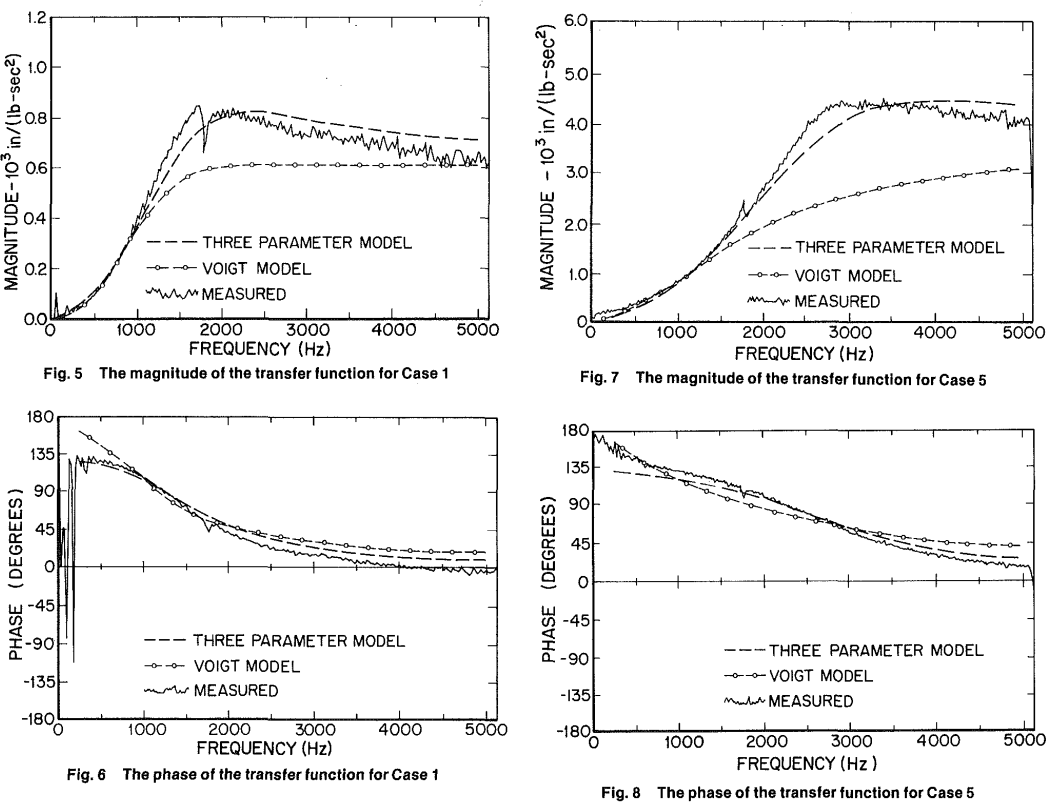
\includegraphics[width=\columnwidth]{bgmodelresults.png}
\end{column}
\begin{column}{0.35\columnwidth}\small
The model we have derived is a model of the form
\[
\begin{array}{c}
\sigma(t) = G_0 \epsilon(t) + G_1 \dot{\epsilon}(t), \\ \epsilon(t) = \frac{x(t)}{\delta} \\
f(t) = m \ddot{x}(t) + f_p(t), \\ f_p(t) = \frac{2A}{\delta}(G_0 + G_1 {}_{CA}D^\alpha x(t)).
\end{array} 
\]
One can do \emph{parameter tuning} to find the fractional order from experimental data
and compare the results with the integer-order model. The results on the left by \cite{BagleyTorvik}
show that the fractional model obtain a better fit with the measured data.
\end{column}
\end{columns}
\end{frame}

\begin{frame}{Equivalent formulations of the Multi-Term FDEs}

In the integer-order case we know how to rewrite the equation
\[
y^{(n)}(t) = f(t,y^{(n-1)}(t),\ldots,y^{(1)}(t),y(t)),  \quad y^{(j)}(0) = y_0^{(j)}, \quad j=0,1,\ldots,n-1,
\]
as a \textbf{system of first-order equations}.

\onslide<2>{\alert{\faQuestionCircle}\, Can we do something similar in the fractional case?}

\begin{itemize}
	\item[(A1)]<3-> Let us assume that our multi-term equation is of the form
	\[
	{}_{CA}D^{\alpha_k} y(t) = f(t,{}_{CA}D^{\alpha_{k-1}} y(t),\ldots,{}_{CA}D^{\alpha_{1}}(t),y(t)),  \quad \begin{array}{l}y^{(j)}(0) = y_0^{(j)}, \\ j=0,1,\ldots,n-1, \end{array}
	\]
	for $\alpha_k > \alpha_{k-1} > \cdots > \alpha_{1} > 0$, $\alpha_j - \alpha_{j-1} \leq 1$ $\forall\,j=1,2,\ldots,k$, $0 < \alpha_1 \leq 1$.
	\item[(A2)]<4-> Assume also that $\alpha_j \in \mathbb{Q}$ $\forall\,j=1,2,\ldots,k$, and that $M$ is the least common multiple of $\alpha_1,\alpha_2,\ldots,\alpha_k$.
\end{itemize}

\end{frame}

\begin{frame}{Equivalent formulations of the Multi-Term FDEs}

\begin{alertblock}{Theorem~\parencite[Theorem~8.1]{DiethelmBook}}
Under the assumptions \alert{(A1)} and \alert{(A2)}, set $\gamma = \nicefrac{1}{M}$, and $N = M \alpha_k$, then the IVP is equivalent to
\[
\begin{cases}
{}_{CA}D^{\gamma} y_0(t) = y_1(t),\\
{}_{CA}D^{\gamma} y_1(t) = y_2(t),\\
\vdots \\
{}_{CA}D^{\gamma} y_{N-2}(t) = y_{N-1}(t),\\
{}_{CA}D^{\gamma} y_{N-1}(t) = f(t,y_0(t),y_{\nicefrac{\alpha_{k-1}}{M}}(t),\ldots,y_{\nicefrac{\alpha_{1}}{M}}(t),y(t)) % ,y_{\nicefrac{\alpha_{k-2}}{M}}(t),
\end{cases} \hspace{-0.5em} y_i(0) = \begin{cases}
y_0^{(\nicefrac{j}{m})}, & \text{ if } \frac{j}{M} \in \mathbb{N}_0,\\
0, & \text{ otherwise}.
\end{cases}
\]
\only<1>{
\begin{itemize}
	\item[$\Rightarrow$] whenever $\mathbf{y} = (y_0,\ldots,y_{N-1})^T$ with $y_0 \in \mathcal{C}^{\lceil \alpha_k \rceil}[0,b]$, for some $b > 0$, is a solution of the $N$-dimensional system, then $y \equiv y_0$ is a solution of the multi-term FDE.
\end{itemize}
}\only<2>{
\begin{itemize}
	\item[$\Leftarrow$] whenever $y \in \mathcal{C}^{\lceil \alpha_k \rceil }([0,b])$ is a solution of the multi-term FDE, then the vector function $\mathbf{y} = (y,{}_{CA}D^{\gamma}y,{}_{CA}D^{2\gamma}y,\ldots,{}_{CA}D^{(N-1)\gamma}y)^T$ solves the $N$-dimensional system.
\end{itemize}
}
\end{alertblock}

\end{frame}

\begin{frame}{Equivalent formulations of the Multi-Term FDEs}

We can relax \alert{(A2)} from the \emph{rationality requirement} to a requirement on being commensurable\footnotemark[2].
\begin{itemize}
	\item[(A2)'] Let $1 \geq \alpha_k > \alpha_{k-1} > \ldots > \alpha_1 > 0$ and assume the equation to be \emph{commensurate}, then we define $\tilde{\alpha}_j = \nicefrac{\alpha_j}{\alpha_1}$ for $j=1,\ldots,k$, let $\tilde{M}$ be the least common multiple of the denominators of the values $\tilde{\alpha}_1,\ldots,\tilde{\alpha}_k$.
\end{itemize} 

\begin{alertblock}{Theorem \parencite[Theorem~8.2]{DiethelmBook}}
Under the assumption \alert{(A1)} and \alert{(A2)'}, set $\gamma = \nicefrac{\alpha_1}{\tilde{M}}$ and $N = \nicefrac{\tilde{M}\alpha_k}{\alpha_1}$, then the equivalence relation of the $N$-dimensional system and of the multi-term FDE holds as in the previous result.
\end{alertblock}

\begin{itemize}
	\item[\faLightbulb]<2-> Existence and uniqueness results can be obtained for the single term reformulation,
	\item[\faCog]<3-> See~\parencite{MR2527892} for other reformulations and comparisons.
\end{itemize}

\footnotetext[2]{Two non-zero real numbers $\alpha$ and $\beta$ are said to be commensurable if their ratio $\nicefrac{\alpha}{\beta} \in \mathbb{Q}$.}

\end{frame}

\section{Partial Differential Equations with Fractional Derivatives with respect to Time}

\begin{frame}{The Method of Lines}

Consider a partial differential equations of the form
\[
\text{Find }u(\mathbf{x},t)\text{ s.t. }u_t = \mathcal{L} u, \quad  \mathbf{x} \in \Omega \subseteq \mathbb{R}^d, t \in I \subseteq \mathbb{R}_+,
\]
where $\mathcal{L}$ is a differential operator, either linear or nonlinear, coupled with the opportune boundary conditions, and given suitable initial conditions.

\onslide<2->{A \emph{classical way} of approaching this task is using a \textbf{Method Of Lines} (MOL) approach, that is
\begin{enumerate}
	\item<2-> we discretize w.r.t. the \emph{space variables} with some method (e.g., Finite Elements/Differences/Volumes, meshfree/meshless methods, spectral methods\ldots)
	\[
	M \mathbf{u}_t = F(t,\mathbf{u}), \quad M \in \mathbb{R}^{n_d \times n_d}, \; F\,:\mathbb{R} \times \mathbb{R}^{n_d} \rightarrow \mathbb{R}^{n_d},\, \mathbf{u} : \mathbb{R} \rightarrow \mathbb{R}^{n_d}.
	\]
	\item<3-> now we have a (possibly nonlinear, non-autonomous) system of ODEs to which we can apply an integrator.
\end{enumerate}
}

\end{frame}

\begin{frame}{PDEs with fractional derivatives with respect to time}
We can think of using the methods we have seen until now for solving PDEs in which the \textbf{derivative with respect to time} has been substituted by the \textbf{fractional derivative in the Caputo sense}
\[
\text{Find }u(\mathbf{x},t)\text{ s.t. } {}_{CA}D^{\alpha} u = \mathcal{L} u, \quad  \mathbf{x} \in \Omega \subseteq \mathbb{R}^d, t \in I \subseteq \mathbb{R}_+.
\]\vfill
\only<2-4>{
\textbf{Examples}:
\begin{itemize}
	\item[\faDiceOne]<2-> Time-fractional diffusion equation
	\[
	{}_{CA}D^{\alpha}_t u = \operatorname{div}(p(x)\operatorname{grad}u) - q(x)u +F(x,t), \quad 0 < \alpha \leq 1.
	\]
	\item[\faDiceTwo]<3-> Time-fractional advection-dispersion equation
	\[
	{}_{CA}D^{\alpha}_t u = \operatorname{div}(p(x)\operatorname{grad}u) - \nu \operatorname{grad}(u), \quad 0 < \alpha \leq 1.
	\]
	\item[\faDiceThree]<4-> Time-fractional  Schr\"{o}dinger equation
	\[
	(i T_\rho)^\alpha {}_{CA}D^{\alpha}_t \psi = - \frac{L^2_\rho}{2 N_m} \nabla^2 \psi + N_\nu \psi, \quad 0 < \alpha \leq 1.
	\]
\end{itemize}
}
\only<5->{
	\textbf{Examples}:
	\begin{itemize}
		\item[\faDiceFive]<5-> Time-fractional Burgers equation equation
		\[
		{}_{CA}D^{\alpha}_t u = u_{xx} + A u^p u_x, \quad 0 < \alpha \leq 1, \; p > 0.
		\]
		\item[\faDiceSix]<6-> Time-fractional Korteweg--de Vries equation
		\[
		{}_{CA}D^{\alpha}_t u = u_{xxx} + A u^p u_x, \quad 0 < \alpha \leq 1, \; p > 0.
		\]
		\item[\faDiceD20]<7-> Time-fractional (incompressible) Navier--Stokes equation
		\[
		\begin{cases}
		{}_{CA}D^{\alpha}_t  (u \cdot \nabla)u = \nu \nabla^2 u - \frac{1}{\rho} \nabla p + f, \\
		\nabla \cdot u = 0.
		\end{cases} \; 0 < \alpha \leq 1.
		\]
	\end{itemize}
}
\end{frame}

\begin{frame}{An example with diffusion}
Let us consider the case of
\[
{}_{CA}D^{\alpha}_t u = 0.05 \nabla^2 u, \quad \alpha = 0.3,1.
\]
and integrate it with the FBDF2 with $\tau = 10^{-2}$.
\begin{center}
\only<1>{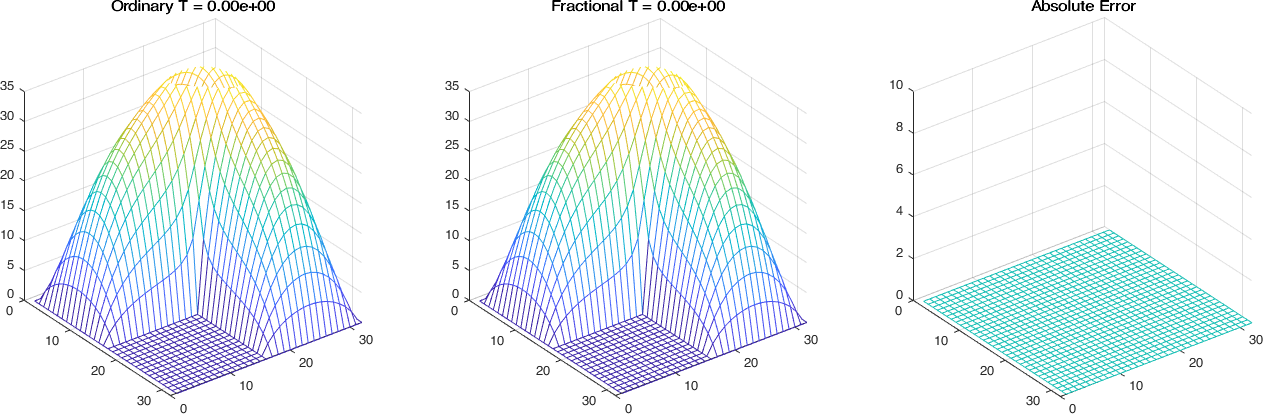
\includegraphics[width=0.9\columnwidth]{diff_001.png}}%
\only<2>{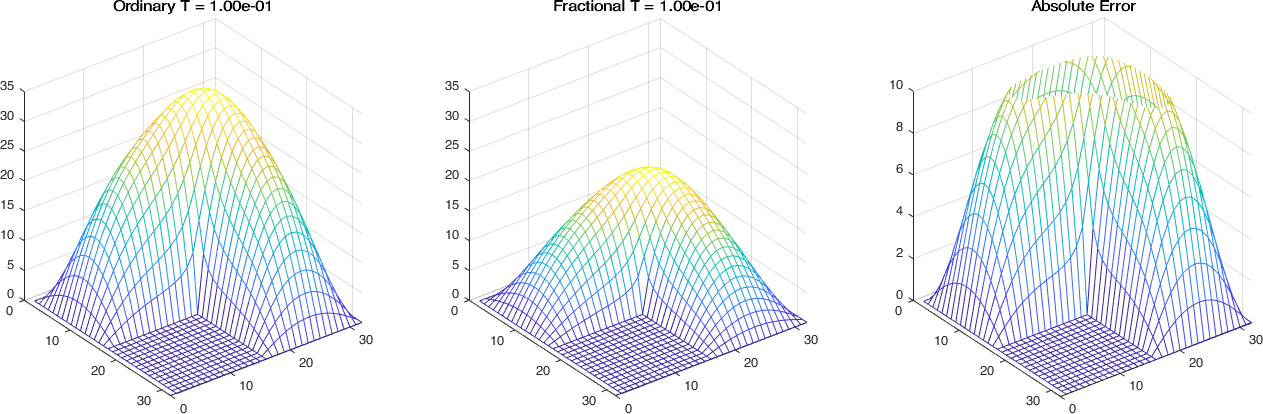
\includegraphics[width=0.9\columnwidth]{diff_011.png}}%
\only<3>{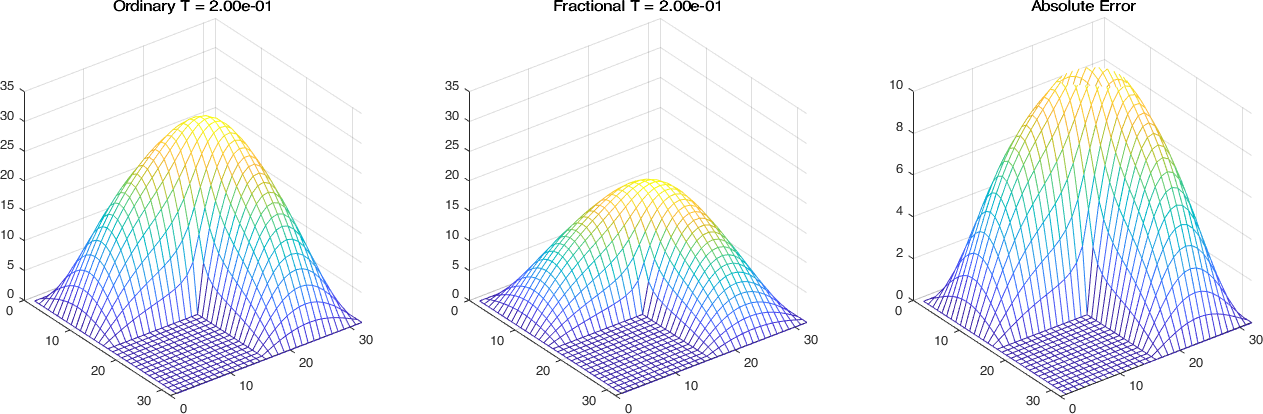
\includegraphics[width=0.9\columnwidth]{diff_021.png}}%
\only<4>{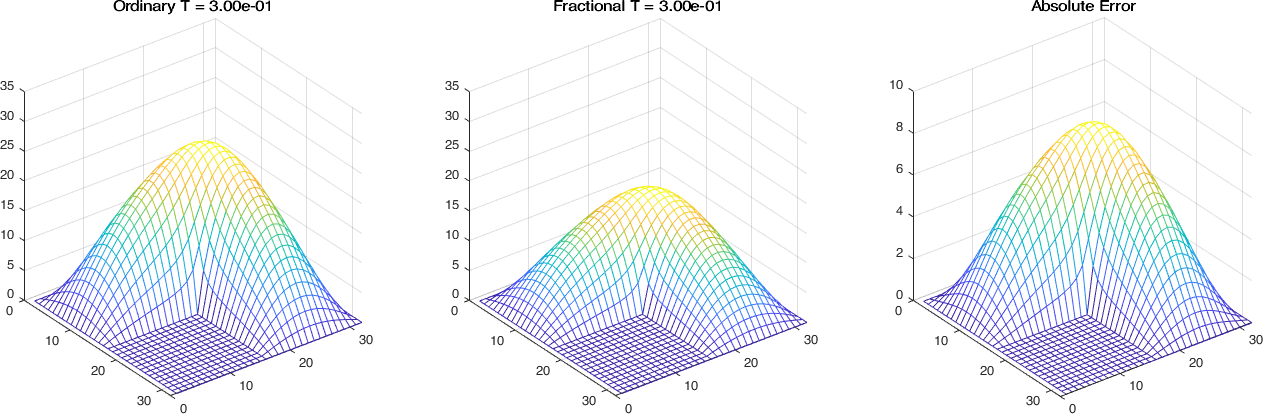
\includegraphics[width=0.9\columnwidth]{diff_031.png}}%
\only<5>{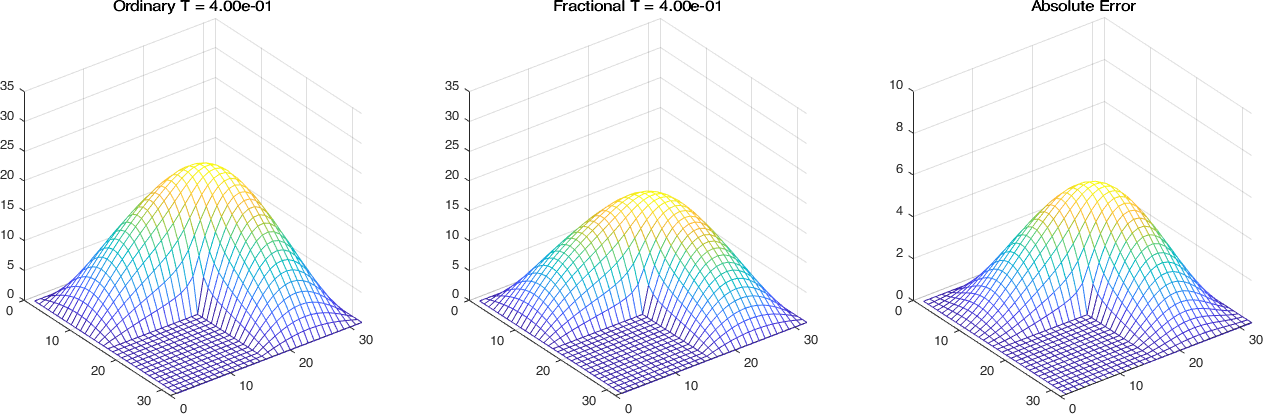
\includegraphics[width=0.9\columnwidth]{diff_041.png}}%
\only<6>{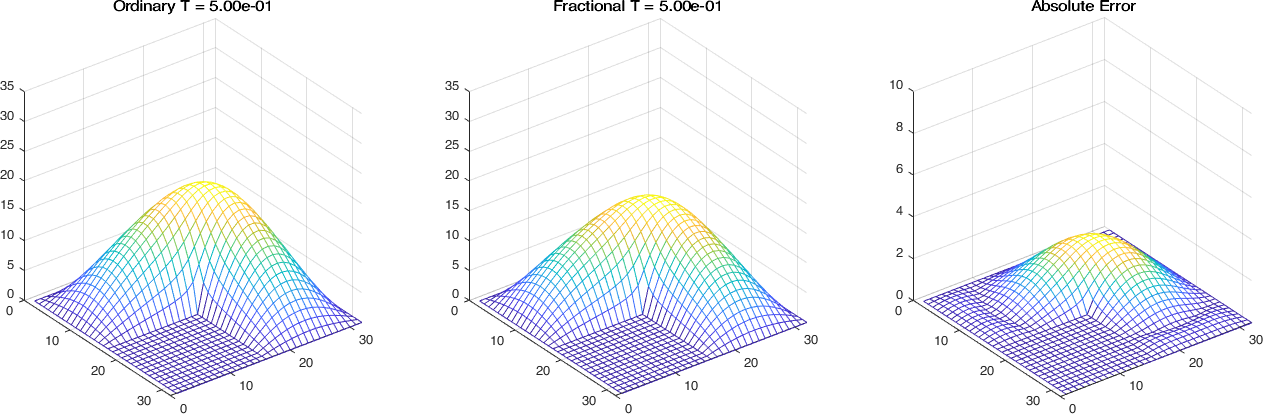
\includegraphics[width=0.9\columnwidth]{diff_051.png}}%
\only<7>{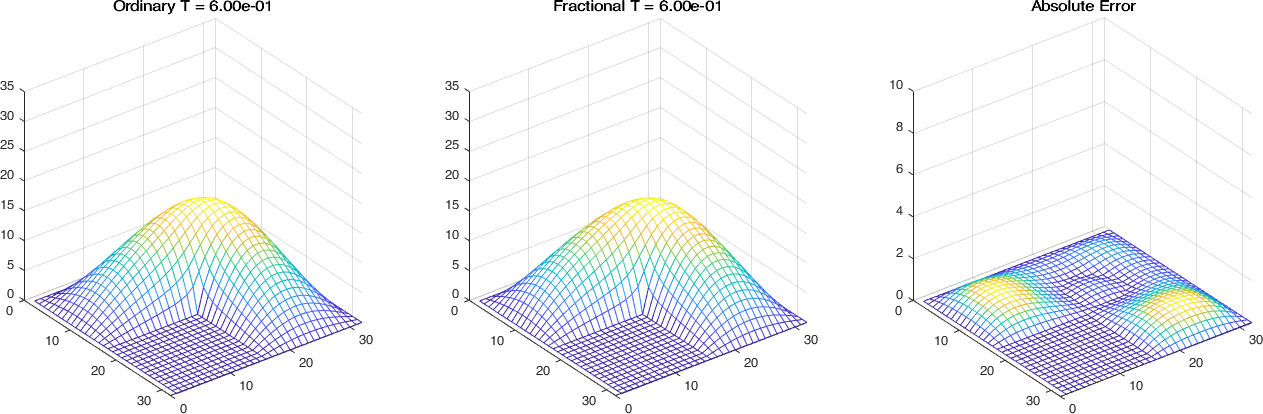
\includegraphics[width=0.9\columnwidth]{diff_061.png}}%
\only<8>{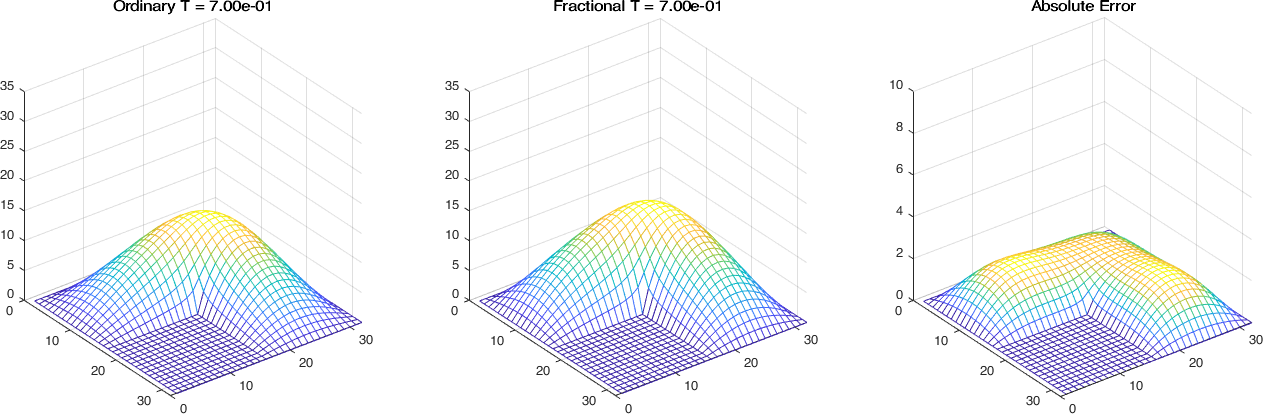
\includegraphics[width=0.9\columnwidth]{diff_071.png}}%
\only<9>{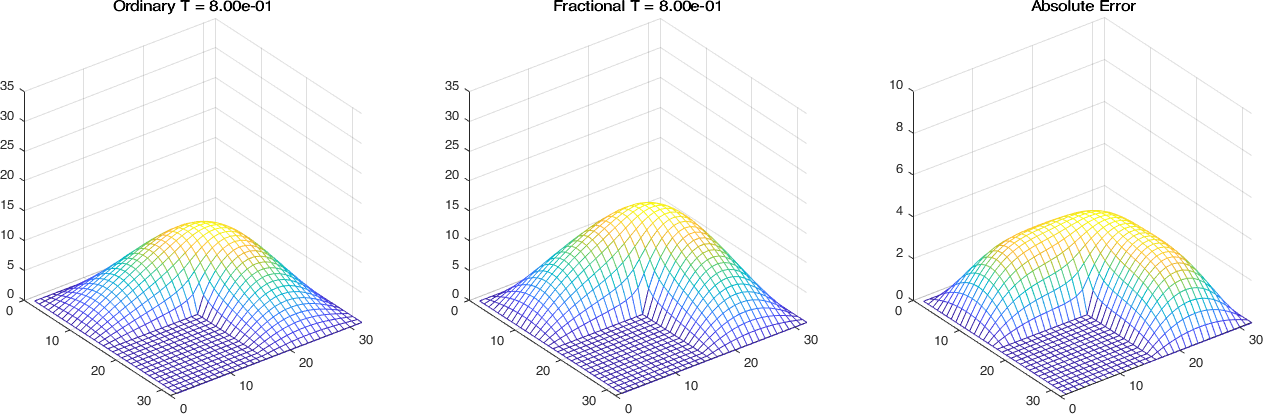
\includegraphics[width=0.9\columnwidth]{diff_081.png}}%
\only<10>{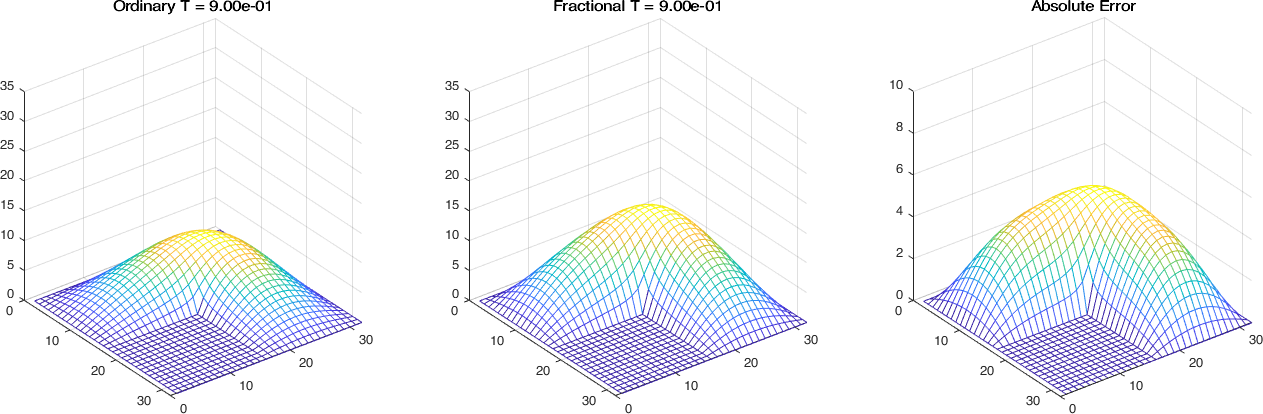
\includegraphics[width=0.9\columnwidth]{diff_091.png}}%
\only<11->{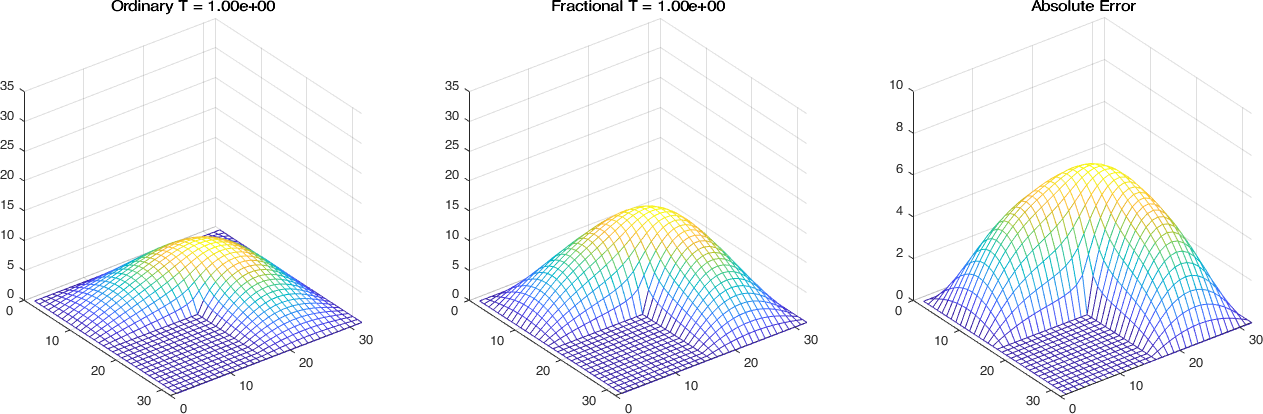
\includegraphics[width=0.9\columnwidth]{diff_101.png}}%
\onslide<12>{ How can you describe the observed behavior? }
\end{center}
\end{frame}

\begin{frame}{Conclusions and next steps}
\definecolor{success}{HTML}{4a934a}
\definecolor{todo}{HTML}{0099cc}

\begin{itemize}
	\item[\textcolor{success}{\faCheckCircle}]<1-> We have completed the construction of several schemes for the integration of FODEs, 
	\item[\textcolor{success}{\faCheckCircle}]<2-> We have discussed the case of FODEs with multiple terms and different orders,
	\item[\textcolor{success}{\faCheckCircle}]<3-> We started looking into some time-fractional PDEs using the Method of Lines together with our FODEs algorithms.
	\item[\textcolor{todo}{\faClipboardList}]<4-> Can we better describe this ``subdiffusive'' behavior we have observed in time-fractional diffusion equation?
	\item[\textcolor{todo}{\faClipboardList}]<5-> For linear problems can we investigate the ``exponential'' fractional integrators?
\end{itemize}

\end{frame}


%\subsection{Fractional-order Chua-Hartley System}
%
%\begin{frame}[fragile]{Fractional-order Chua-Hartley System}
%\begin{columns}
%\begin{column}{0.4\columnwidth}
%\centering
%
%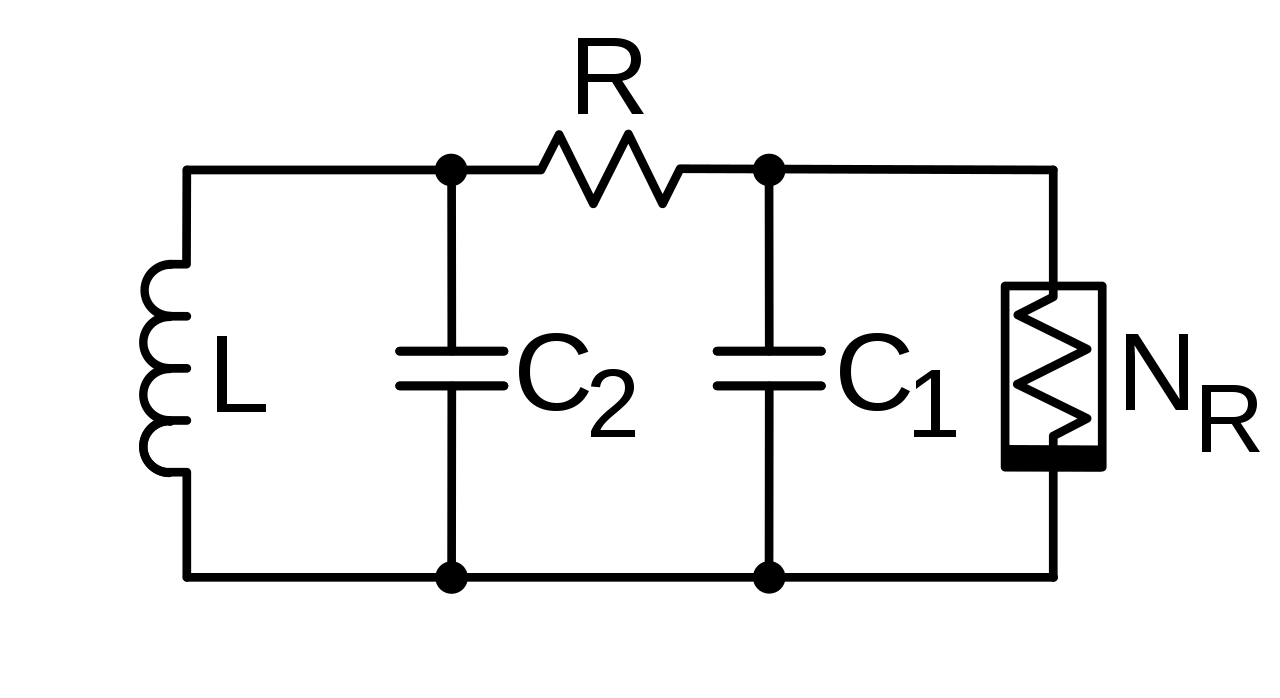
\includegraphics[width=\columnwidth]{chua.png}	
%
%\begin{itemize}
%\item \small $L$ is an \emph{inductor},
%\item \small $C_1$ and $C_2$ are two \emph{capacitors},
%\item \small $R$ is a \emph{resistance},
%\item \small $N_R$ is is a \textbf{nonlinear} negative resistance\footnotemark[1] called a \emph{Chua's diode}.
%\end{itemize}
%\end{column}
%\begin{column}{0.6\columnwidth}
%If we write down the equation for the currents in the system
%\[
%\begin{cases}
%\dot{x} = \alpha \left[y + \frac{x-2x^3}{7}\right],\\
%\dot{y} = x-y+z,\\
%\dot{z} = -\beta y,
%\end{cases}
%\]
%where $x(t)$ and $y(t)$ represent the \textbf{voltages} across the capacitors $C_1$ and $C_2$, while $z(t)$ represents the 
%\textbf{electric current} in the inductor $L_1$. 
%\vfill
%
%\begin{quote}\footnotesize
%	\faFile*\;\fullcite{hartley1995chaos}
%\end{quote}
%
%\end{column}
%\end{columns}
%\footnotetext[1]{It causes an increase in voltage across the terminals and thus a decrease in electric current through it.}
%\end{frame}
%
%\begin{frame}{Fractional-order Chua-Hartley System}
%\begin{columns}
%\begin{column}{0.4\columnwidth}
%\centering
%
%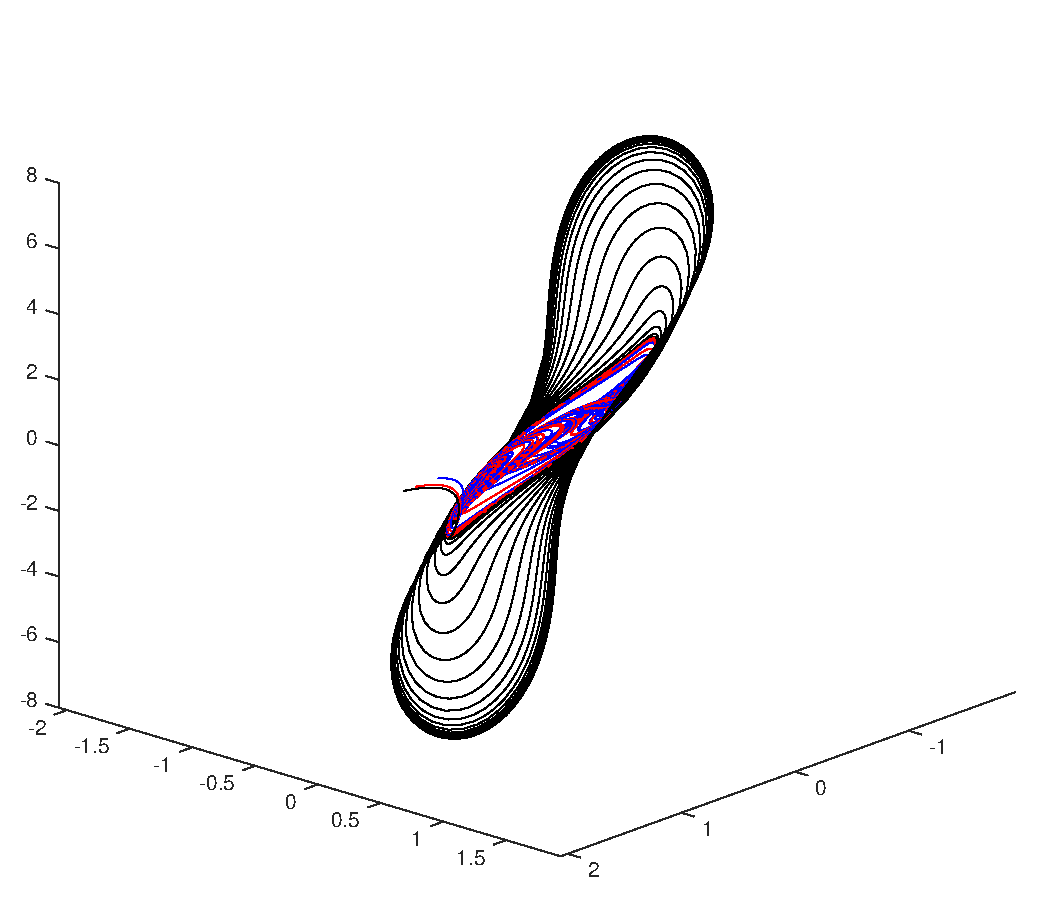
\includegraphics[width=\columnwidth]{ordinarysystem.eps}
%\end{column}
%\begin{column}{0.6\columnwidth}
%	contenuto...
%\end{column}
%\end{columns}
%\end{frame}

%\begin{frame}[fragile]{The FRF first implementation}
%
%\begin{columns}
%\begin{column}{0.6\columnwidth}\definecolor{bg}{rgb}{0.95,0.95,0.95}
%The code is analogous to the one for the fractional integrals 
%with Newton-Cotes formulas:
%\begin{minted}[bgcolor=bg,fontsize=\small,breaklines]{matlab}
%for i=0:N-1
%% These are the values b0,b1,...,bN-1 we need 
%% them for all the computations
%b(i+1) = ((i+1)^alpha - i^alpha)/alpha; 
%end
%y(:,1) = y0;
%c = (tau^alpha/gamma(alpha));
%for j=1:N-1
%fy(:,j) = f(t(j),y(:,j)); % New value of f
%y(:,j+1) = y(:,1) + c*sum(flipud(b(1:j)).'.*fy(:,1:j));
%end
%\end{minted}
%\end{column}
%\begin{column}{0.4\columnwidth}
%\begin{itemize}
%\item[\faCode]<2-> To build the solution we have to keep in memory either the \textbf{previous solutions} or the \textbf{function evaluations},
%\item[\faCode]<3-> We have to compute:
%\[
%\sum_{j=0}^{n-2} b_{n-j-1}f^{(j)},
%\]
%this is a \alert{quadratic cost} with $N$.
%\item<4-> The $1$-step name is related to the number of initial values to start the computation.
%\end{itemize}
%\end{column}
%\end{columns}
%
%\end{frame}
%
%\begin{frame}[fragile]{The FRF consistency order}
%\begin{columns}
%\begin{column}{0.5\columnwidth}
%We need to investigate the order of approximation of this method.
%
%If we apply it to the case
%\[
%{}_{CA}D_{[0,t]}^\alpha y(t) = \lambda y(t), \quad y(0) = 0,
%\]
%for $t \in [0,]
%\end{column}
%\begin{column}{0.5\columnwidth}
%\centering
%
%\input{fprerror.tikz}
%	
%\begin{tabular}{ll}
%\toprule
%$\tau$ & Error\\
%\midrule
%5.00e-01 & 5.07e-02\\
%1.00e-01 & 8.17e-03\\
%1.00e-02 & 6.83e-04\\
%1.00e-03 & 6.40e-05\\
%\bottomrule
%\end{tabular}
%
%\end{column}
%\end{columns}
%\end{frame}
%
%\begin{frame}{The Fractional Trapezoidal Formula}
%
%\end{frame}
%
%\section{Fractional Linear Multistep Methods}
%
%\begin{frame}{Fractional Linear Multistep Methods}
%To 
%\end{frame}

\appendix

\section*{Bibliography}
{\unnumbered
	\begin{frame}[allowframebreaks,noframenumbering]{Bibliography}
	\small
	\printbibliography
	
\end{frame}
}

\end{document}